% !TeX program = xelatex
% SPDX-License-Identifier: CC-BY-4.0
\documentclass[11pt,openany]{book}
% SPDX-License-Identifier: MIT
\usepackage{fontspec}
\setmainfont{texgyrepagella-regular.otf}[
  BoldFont=texgyrepagella-bold.otf,
  ItalicFont=texgyrepagella-italic.otf,
  BoldItalicFont=texgyrepagella-bolditalic.otf]
\setsansfont{texgyreheros-regular.otf}[
  BoldFont=texgyreheros-bold.otf,
  ItalicFont=texgyreheros-italic.otf,
  BoldItalicFont=texgyreheros-bolditalic.otf]
\setmonofont{lmmono10-regular.otf}[Scale=MatchLowercase]
\usepackage[paperwidth=170mm,paperheight=240mm,inner=20mm,outer=18mm,top=20mm,bottom=22mm,headheight=15pt]{geometry}
\usepackage{graphicx,booktabs,tabularx,longtable,array}
\usepackage{amsmath,amssymb}
\usepackage{enumitem}
\usepackage{xcolor}
\definecolor{BookTeal}{HTML}{176C68}
\definecolor{BookInk}{HTML}{23363E}
\definecolor{BookRule}{HTML}{C8D6D6}
\definecolor{BookPale}{HTML}{F1F6F5}
\usepackage{tikz}
\usetikzlibrary{arrows.meta,positioning,shapes.geometric,shapes.misc,fit,backgrounds,calc,matrix}
\usepackage{rotating}
\usepackage{pdfpages}
\usepackage{fvextra}
\DefineVerbatimEnvironment{Prompt}{Verbatim}{fontsize=\small,breaklines=true,breakanywhere=true,frame=single,rulecolor=\color{BookRule},framesep=2mm}
\usepackage{caption}
\captionsetup{font=small,labelfont=bf,labelsep=period}
\usepackage{fancyhdr}
\pagestyle{fancy}
\fancyhf{}
\fancyhead[LE,RO]{\small\thepage}
\fancyhead[LO,RE]{\small\nouppercase{\leftmark}}
\renewcommand{\headrulewidth}{0.3pt}
\usepackage{xurl}
\usepackage[unicode,hypertexnames=false,colorlinks=true,linkcolor=BookTeal,urlcolor=BookTeal,citecolor=BookTeal,breaklinks=true]{hyperref}
\usepackage{bookmark}
\setcounter{tocdepth}{1}
\setcounter{secnumdepth}{1}
\let\cleardoublepage\clearpage
\setlist{nosep,leftmargin=1.8em}
\renewcommand{\arraystretch}{1.25}
\setlength{\parskip}{0.3em}
\setlength{\emergencystretch}{2em}
\newcommand{\bookversion}{0.1.0}
\newcommand{\bookdate}{2026-10-29}
\newcommand{\scidraw}{SciDraw AI}
% Drawn marks: the book fonts lack U+2713/U+2715.
\newcommand{\bookcheck}{\tikz[x=1em,y=1em,baseline=-0.1em,line width=0.12em,line cap=round,line join=round]\draw[color=.] (0,0.3)--(0.28,0)--(0.75,0.7);}
\newcommand{\bookcross}{\tikz[x=1em,y=1em,baseline=-0.1em,line width=0.12em,line cap=round]{\draw[color=.] (0,0)--(0.6,0.65);\draw[color=.] (0,0.65)--(0.6,0);}}
% Circled numbers and the inhibition sign are missing from the book fonts; draw them.
\usepackage{newunicodechar}
\newcommand{\bookcirc}[1]{\tikz[baseline=(n.base)]\node[circle,draw,inner sep=0.5pt,minimum size=1.05em,font=\sffamily\scriptsize] (n) {#1};}
\newcommand{\bookcircfill}[1]{\tikz[baseline=(n.base)]\node[circle,fill,inner sep=0.5pt,minimum size=1.05em,font=\sffamily\scriptsize\bfseries,text=white] (n) {#1};}
\newunicodechar{①}{\bookcirc{1}}
\newunicodechar{②}{\bookcirc{2}}
\newunicodechar{③}{\bookcirc{3}}
\newunicodechar{④}{\bookcirc{4}}
\newunicodechar{⑤}{\bookcirc{5}}
\newunicodechar{⑥}{\bookcirc{6}}
\newunicodechar{⑦}{\bookcirc{7}}
\newunicodechar{⑧}{\bookcirc{8}}
\newunicodechar{⑨}{\bookcirc{9}}
\newunicodechar{⑩}{\bookcirc{10}}
\newunicodechar{⑪}{\bookcirc{11}}
\newunicodechar{⑫}{\bookcirc{12}}
\newunicodechar{⑬}{\bookcirc{13}}
\newunicodechar{❶}{\bookcircfill{1}}
\newunicodechar{❷}{\bookcircfill{2}}
\newunicodechar{❸}{\bookcircfill{3}}
\newunicodechar{❹}{\bookcircfill{4}}
\newunicodechar{❺}{\bookcircfill{5}}
\newunicodechar{❻}{\bookcircfill{6}}
\newunicodechar{❼}{\bookcircfill{7}}
\newunicodechar{⊣}{\ensuremath{\dashv}}
\providecommand{\sdbase}{https://sci-draw.com}
\newcommand{\sdtool}[1]{\href{\sdbase/#1}{\texttt{/#1}}}
\newcommand{\bookrepo}{https://github.com/TopLocalAI/ai-scientific-figures-book}
\newenvironment{BookNote}{\begin{quote}\small\color{BookInk}}{\end{quote}}
\newcolumntype{Y}{>{\raggedright\arraybackslash}X}
\newcommand{\workflowfigure}[2]{%
  \begin{figure}[htbp]\centering
  \input{figures/workflow-#1.tex}
  \caption{#2}\label{fig:workflow}
  \end{figure}}
\newcommand{\pairedfigure}[2]{%
  \begin{figure}[htbp]\centering
  \includegraphics[width=\linewidth]{figures/paired-comparison-#1.pdf}
  \caption{#2}\label{fig:paired}
  \end{figure}}

\hypersetup{pdftitle={Use AI to Make Better Scientific Figures: From Research Ideas to Paper Figures},pdfauthor={TopLocalAI contributors},pdflang={en}}
\begin{document}
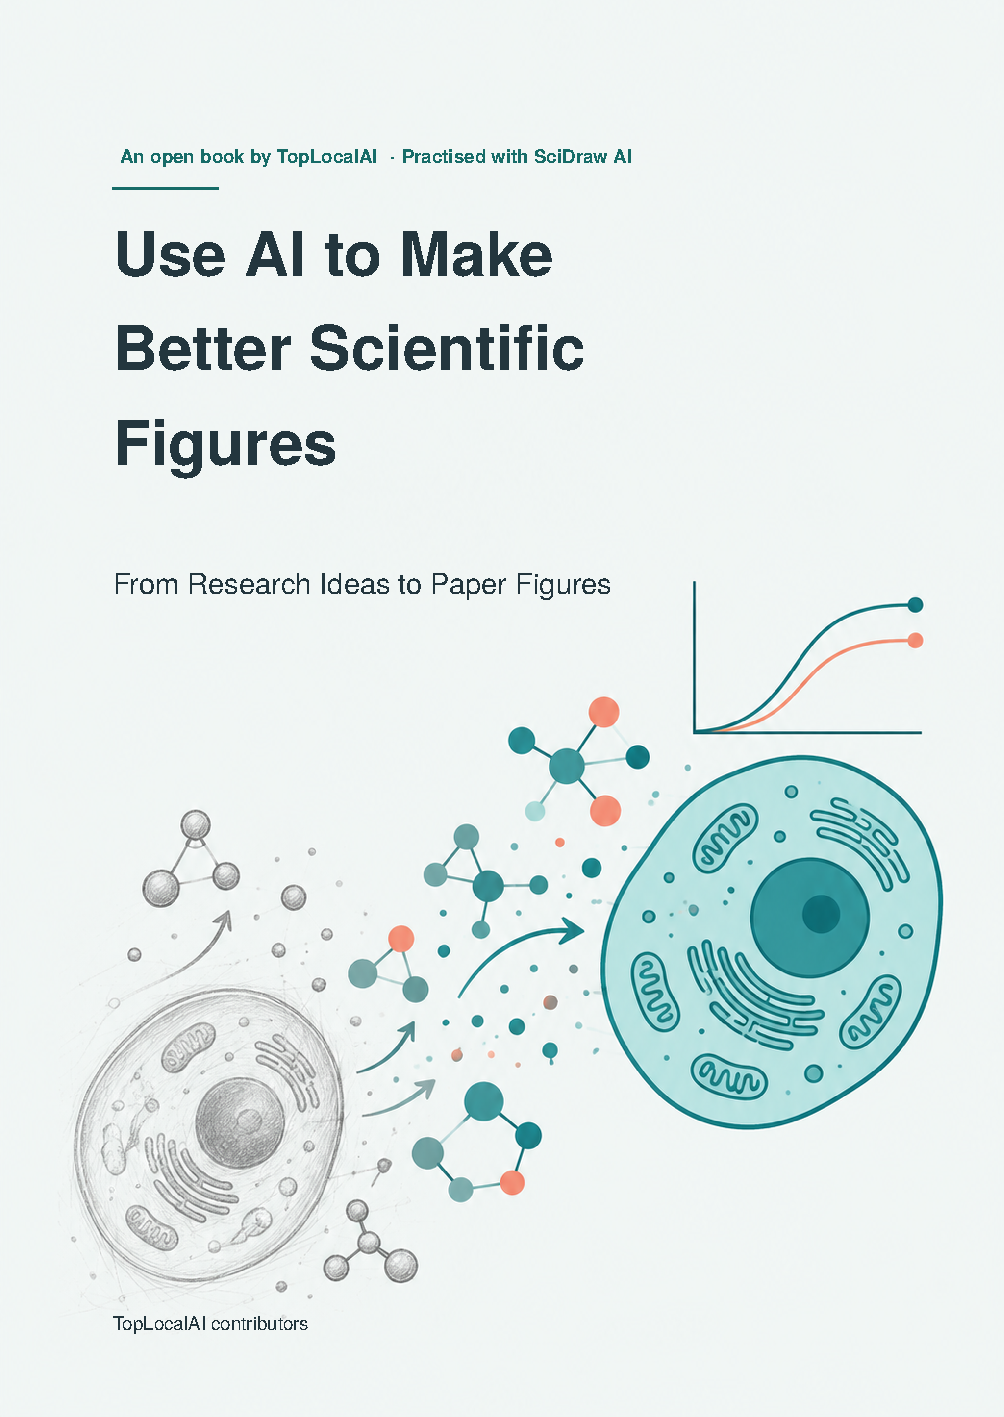
\includepdf[pages=1,fitpaper=false,noautoscale=false]{cover/cover-en.pdf}
\begin{titlepage}
\color{BookInk}
\vspace*{18mm}
{\sffamily\large An open book by TopLocalAI\par}
\vspace{18mm}
{\Huge\bfseries Use AI to Make Better Scientific Figures\par}
\vspace{8mm}
{\Large From Research Ideas to Paper Figures\par}
\vspace{14mm}
{\large Practical workflows with SciDraw AI\par}
\vfill
{\large English edition · v\bookversion\par}
\vspace{3mm}
{\normalsize \bookdate\par}
\vspace{8mm}
\end{titlepage}
\frontmatter
\chapter*{Version and use}
This open book is maintained by TopLocalAI in LaTeX, with Chinese and English editions. It has thirteen chapters, a preface, and appendices.

\scidraw{} (\href{https://sci-draw.com}{sci-draw.com}) provides the practical workflow used throughout the book. The tools referred to in the text are listed below; in the PDF every tool name is a clickable link.

\begin{center}\small
\begin{tabular}{@{}ll@{}}
Prompt drawing, sketches, reference-image edits & \href{https://sci-draw.com/ai-drawing}{sci-draw.com/ai-drawing}\\
Mechanism figures & \href{https://sci-draw.com/mechanism-figure-generator}{sci-draw.com/mechanism-figure-generator}\\
Workflow diagrams & \href{https://sci-draw.com/workflow-diagram-generator}{sci-draw.com/workflow-diagram-generator}\\
Data visualization & \href{https://sci-draw.com/sci-vis}{sci-draw.com/sci-vis}\\
Multi-panel figures & \href{https://sci-draw.com/multi-panel-figure-maker}{sci-draw.com/multi-panel-figure-maker}\\
Graphical abstracts & \href{https://sci-draw.com/graphical-abstract-maker}{sci-draw.com/graphical-abstract-maker}\\
Figure legends & \href{https://sci-draw.com/figure-legend}{sci-draw.com/figure-legend}\\
Figure checks & \href{https://sci-draw.com/figure-checker}{sci-draw.com/figure-checker}\\
Figure workflow guide (links the tools above) & \href{https://sci-draw.com/figure-workflow}{sci-draw.com/figure-workflow}\\
\end{tabular}
\end{center}

Example illustrations were made with an image-generation model; data figures come from public datasets or clearly labelled simulated data, rendered by scripts that ship with the book. The actual tool, prompt, and revision history of every figure are recorded in the book repository.

The manuscript, original teaching data, and figures are offered under \href{https://creativecommons.org/licenses/by/4.0/}{CC BY 4.0}. Build scripts, plotting code, and shared typesetting code use the MIT license. See LICENSE, ASSETS.md, and the provenance directory for scope and source details. Product names and trademarks are not transferred by these licenses.

Suggested citation: TopLocalAI contributors. \emph{Use AI to Make Better Scientific Figures: From Research Ideas to Paper Figures}. v\bookversion, \bookdate.

\url{https://github.com/TopLocalAI/ai-scientific-figures-book}
\begingroup\small\linespread{1.0}\selectfont
\setlength{\parskip}{0pt}
\tableofcontents
\endgroup
\chapter*{Preface: Bring attention back to the research}
\addcontentsline{toc}{chapter}{Preface}
\markboth{Preface}{Preface}

We often leave figures until the final stages of writing a paper. The data have been analyzed, the methods are documented, and the conclusions seem clear. All that remains is to make the figures look good. Once we begin, problems appear: one image cannot hold everything, two arrows invite different interpretations, a summary hides individual variation, and text that looked clear on a monitor becomes unreadable at its final size.

These difficulties are closely connected to the research. Making a figure requires us to decide again what matters most, which elements are evidence, which are interpretation, and in what order the reader should encounter them. Sometimes a figure is unclear because its layout has not been resolved. Sometimes the question it should answer has not yet been stated precisely.

AI lowers the effort needed to begin. We can describe a scene in words, suggest a composition with a sketch, explain a revision using an existing image, or give data to a visualization tool and explore ways to present them. Tasks that once required many separate operations can now start with a short instruction. That creates more room to compare alternatives and refine the explanation.

A polished image can also conceal mistakes. An incorrect relationship can look convincing. A tidy layout can distract from a missing experimental condition. An unsupported conclusion can acquire a professional-looking visual form. We therefore need to move from being able to generate a figure to being able to explain, inspect, and deliver it.

This book follows that process. You will begin with a drawing brief that states the purpose of the figure and the question it should answer. You will then choose a workflow for a data plot, a methods diagram, a mechanism illustration, an experimental image, or a graphical abstract. We will discuss composition, color, labels, and legends, as well as revision, export, and preservation of source materials. Each part explains what AI can assist with and what must be decided from the research record.

SciDraw AI is the practical platform used throughout the book. A common platform lets readers continue working on the same example without repeatedly learning a new interface. Instructions are based on actual interfaces and available operations. Where a workflow requires a download, an upload, or a manual addition, that step is stated directly. Features enter a tutorial after they have been implemented and checked.

You do not need to master illustration before starting. More useful preparation is a study you understand, a complete set of source materials, and a willingness to inspect each important element. Experienced readers can enter at a specific problem: retaining the study design in a data plot, reducing ambiguity in a mechanism diagram, or arranging several panels into a readable argument.

Exercises distinguish simulated materials from real research. Simulated data allow us to share a reproducible task and discuss mistakes without presenting a teaching result as a scientific discovery. Real cases require reliable sources and any necessary permission. The aim is a method that transfers to your own work: decide what to communicate, use the tools, and preserve important decisions together with their basis.

In the next chapter, focus on one concrete question: what should this figure help the reader understand?

\mainmatter
\chapter{Building Your AI Workflow for Scientific Figures}
\usetikzlibrary{decorations.pathreplacing}

Lin, a graduate student in environmental science, is drafting a paper on seasonal variations in river nitrate across an agricultural watershed. Figure 2 of her manuscript has to accomplish two things at once. First, it must orient readers to the spatial pathway through which water and solutes move across the basin: from row-crop fields into subsurface tile drains, out through a tributary drainage ditch, into the main river channel, and down to a stream-monitoring gauge. Second, it must present the full-year 2016 daily record of river nitrate concentration alongside stream discharge at that gauge. Looking over her outline, her advisor leaves a single margin note: ``Put the full year of monitoring data and the study area into one figure so readers can immediately see how concentration relates to flow.''

Lin opens a plotting tool, uploads the daily mean table she downloaded from the U.S. Geological Survey (USGS), and types a one-sentence request: ``Help me turn these river data into a professional paper figure that highlights the nitrate pollution problem.'' Less than a minute later, a colorful chart appears on her screen (Figure~\ref{fig:ch01-03} reconstructs a typical result of this kind of prompt). At a casual glance, the plot looks ready to drop into a manuscript. The moment she sits down to write the figure legend, however, one defect after another comes to light. Nitrate concentration and river discharge are plotted on twin vertical axes in bright red and green; wherever the two curves cross, the intersection invites the false impression that concentration and flow are ``equal'' on that date. Two days in mid-September when the in-situ sensor was offline have been bridged seamlessly by a straight line. The left vertical axis is labeled simply ``Nitrate (mg/L)'' without stating whether mass is reported as elemental nitrogen ($\text{mg/L as N}$) or as the whole nitrate ion ($\text{NO}_3^-$). Worse still, a thick red horizontal line at $10\ \text{mg/L}$ is stamped ``Exceeds limit!'', even though that regulatory threshold applies to treated public drinking water rather than untreated river water.

Hoping for better luck with the study-area panel, she types a one-line English prompt into an image generator to illustrate nitrate pollution in an agricultural watershed (Figure~\ref{fig:ch01-05}). The resulting picture looks like a polished textbook spread, yet the model has populated the riverbank with a municipal water-treatment complex, painted green algal blooms across the foreground channel, and added an inset diagram explaining how decomposing algae deplete dissolved oxygen---none of which she measured or studied in her paper.

With a single vague sentence, the author handed over a dozen scientific decisions to software that knows nothing about her sampling protocol, her quality flags, or the scope of her claims. This chapter addresses that root problem: before typing prompts or running scripts, we need a reliable workflow that keeps every scientific decision in the author's hands.

\section{Give the figure a task you can check}

Every figure in a research paper exists to perform one primary job. That job might be to trace the physical pathway connecting agricultural drainage to a downstream gauge, to show how two hydrochemical variables co-vary across the twelve months of a year, or to compare paired measurements on the same subjects before and after a treatment. Whatever the subject matter, the stated goal must be specific enough to constrain three concrete design choices: chart type, spatial layout, and labels.

A vague intention such as ``show the 2016 monitoring results'' fails as a design specification because it cannot rule out bad choices. Collapsing 366 daily observations into a single annual mean bar ``shows the monitoring results.'' Linearly interpolating across instrument outages, omitting the chemical reporting basis, or plotting two incompatible quantities on arbitrary twin axes also ``shows the monitoring results.'' Once you rewrite the task as a testable statement, however, the boundaries of acceptable design snap into focus.

Starting from the audience and the message rather than from software menus is a basic principle of scientific visualization. In their ten simple rules for better figures, Rougier, Droettboom, and Bourne (2014) place ``Know Your Audience'' and ``Identify Your Message'' ahead of every stylistic consideration. Throughout this book, we turn those two rules into a single sentence that you fill in before opening any tool:

\begin{BookNote}
After viewing this figure, the reader should be able to understand \rule{25mm}{0.3pt}, and be able to locate \rule{25mm}{0.3pt} in the figure.
\end{BookNote}

The two halves of this template perform distinct jobs. The first blank defines the interpretive purpose of the figure: the conceptual relationship or empirical pattern that a colleague should grasp after studying it. The second blank lists the concrete visual elements that the reader---and you during quality control---must be able to point to and verify on the page. Notice that a well-formed task sentence never forces the data to tell a predetermined story; instead, it requires the figure to accommodate all observed facts honestly.

Consider what happens when Lin rewrites her goal for the Raccoon River data panel using this template:

\begin{BookNote}
After viewing this figure, the reader should be able to understand the seasonal variation of nitrate concentration in the Raccoon River during 2016 and its temporal covariation with stream discharge, and be able to locate the daily mean values, missing-data days, the 10 mg/L (as N) reference line, and the winter periods of ice-affected estimated discharge in the figure.
\end{BookNote}

That single sentence settles most of the structural decisions for her data plot before she touches a keyboard:
\begin{itemize}
\item \textbf{It determines the chart type:} Requiring the reader to locate ``daily mean values'' and ``missing-data days'' rules out monthly bar charts or seasonal box plots. The plot must preserve the daily time series and break cleanly wherever observations are missing, without smoothing filters or linear interpolation.
\item \textbf{It determines the layout:} Assessing ``temporal covariation'' between two variables with incompatible physical dimensions---concentration in $\text{mg/L}$ versus discharge in $\text{m}^3/\text{s}$ spanning nearly two orders of magnitude---calls for two vertically stacked subplots sharing a common horizontal time axis. Readers can scan vertically to compare hydrograph peaks with concentration responses on the same date, avoiding the arbitrary curve crossings of a dual-Y-axis plot.
\item \textbf{It determines the labels and annotations:} Naming ``the 10 mg/L (as N) reference line'' and ``winter periods of ice-affected estimated discharge'' reminds the author that the vertical axis must state ``as N,'' the horizontal benchmark must be annotated as a drinking-water standard shown for reference only, and winter flow values estimated under ice cover must be visually distinguished from regular open-water measurements.
\end{itemize}

The same logic applies to other study designs. Suppose you have paired measurements on a cohort of subjects before and after an intervention. If your task sentence states that the reader should ``understand whether individual subjects change in a consistent direction between the two conditions, and be able to locate all paired observations as well as any individual moving opposite to the group trend,'' then a bar chart showing only group means and standard deviations is eliminated immediately. Only a plot that preserves individual trajectories---such as a paired dot-and-line plot---meets the requirement (Weissgerber et al., 2015). Chapters 2 and 5 use this paired-data scenario to show how study design governs statistical graphics.

Whenever you find yourself struggling to fill in the second blank---unable to name the exact elements a reader should be able to locate---the underlying analytical point of the figure is usually still fuzzy. Stopping to sharpen that sentence saves far more time than running twenty trial-and-error prompts in a plotting tool. Chapter 2 shows how to expand this one-sentence task into a complete drawing brief.

\section{Know what kind of material you have}

Once you have written a testable task sentence, the second step is to inventory your raw materials. For practical figure production, we group scientific inputs into three operational categories: (1) numerical data and tables, (2) explanatory content (text descriptions, sketches, and established relationships), and (3) images acquired from laboratory instruments or field sites. This classification guides tool selection and defines verification duties. A single paper---and often a single multi-panel figure---routinely combines all three.

\begin{center}\footnotesize
\setlength{\tabcolsep}{3pt}
\renewcommand{\arraystretch}{1.15}
\begin{tabularx}{\linewidth}{@{}>{\raggedright\arraybackslash}p{24mm}>{\raggedright\arraybackslash}p{26mm}YY@{}}
\toprule
\textbf{Material category} & \textbf{What the figure expresses} & \textbf{Counterpart and tool route in this case} & \textbf{What the author must verify} \\
\midrule
Numerical data and tables & Quantities, distributions, temporal trends, and relationships among variables & USGS station 05484500 daily mean nitrate and discharge table for 2016; use a deterministic plotting script or \scidraw{} scientific visualization (\sdtool{sci-vis}) to produce panel b & Raw numerical values, measurement units, line breaks at missing days, quality-code flags, axis transformations, and statistical meaning \\
Text, sketches, and confirmed relationships & Spatial setting, experimental protocols, mechanistic pathways, and conceptual frameworks & Literature and station descriptions of cropland subsurface tile drainage entering the river upstream of the gauge; use \scidraw{} to generate a text-free base illustration and overlay vector labels to form panel a & Included and excluded objects, object counts, flow or action directions, boundary conditions, and absence of unsupported pollution sources or mechanisms \\
Instrument or field images & Observed morphology, gel bands, microscopic signals, or spatial field evidence & (If included in a study) field photographs of sensor installation or remote-sensing imagery; preserve original files and use non-destructive presentation and panel assembly (not used in this case) & Unaltered raw file backups, scale-bar calibration, channel and crop records, cross-batch comparability, and strict prohibition of generative beautification \\
\bottomrule
\end{tabularx}
\end{center}

Why make this classification before opening software? Because different materials carry fundamentally different \textbf{evidential roles} in a paper, and therefore demand different production tools and red-line constraints (Figure~\ref{fig:ch01-02}).

\begin{figure}[htbp]\centering
\resizebox{\linewidth}{!}{\providecommand{\route}[1]{{\scriptsize\color{BookTeal}#1}}
\providecommand{\authcheck}[1]{{\scriptsize\color{BookInk!75}#1}}
\begin{tikzpicture}[
  card/.style={draw=BookTeal,fill=BookPale,rounded corners=2pt,text width=39mm,align=center,font=\small,minimum height=62mm},
  cardunused/.style={card,dashed,draw=gray,text=BookInk!80},
  route/.style={font=\scriptsize,text=BookTeal},
  check/.style={font=\scriptsize,text=BookInk!75},
  bracebox/.style={draw=BookInk,rounded corners=1pt,font=\small,inner sep=3pt}
]
\node[card] (d) at (0,0) {%
  \begin{tikzpicture}[scale=0.55,baseline=(t.base)]
    \foreach \x in {0,1,2} {
      \foreach \y in {0,1,2} {
        \draw[BookInk!60] (\x*0.35,\y*0.28) rectangle ++(0.32,0.24);
      }
    }
    \coordinate (t) at (0.35,0.5);
  \end{tikzpicture}\\[2mm]
  Data\\[1mm]
  USGS daily means\\(nitrate, discharge)\\[2mm]
  {\route Deterministic plotting / sci-vis → panel b}\\[2mm]
  {\authcheck Author checks: raw values, units, gaps, quality codes}};
\node[card,right=7mm of d] (i) {%
  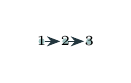
\begin{tikzpicture}[scale=0.55,baseline=(c.base)]
    \foreach \x/\n in {0/1,1/2,2/3} {
      \fill[BookTeal!40] (\x*0.55,0.15) circle (0.07);
      \node at (\x*0.55,0.15) {\tiny\n};
    }
    \draw[-{Stealth},BookInk] (0.07,0.15)--(0.43,0.15);
    \draw[-{Stealth},BookInk] (0.62,0.15)--(0.98,0.15);
    \coordinate (c) at (0.55,0.15);
  \end{tikzpicture}\\[2mm]
  Explanatory content\\[1mm]
  Study-area and drainage-path description\\[2mm]
  {\route Image generation → panel a}\\[2mm]
  {\authcheck Author checks: objects, flow, unsupported sources}};
\node[cardunused,right=7mm of i] (p) {%
  
\begin{tikzpicture}[scale=0.55,baseline=(cam.base)]
    \draw[BookInk!70,rounded corners=1pt] (0,0.05) rectangle (0.55,0.38);
    \draw[BookInk!70] (0.55,0.28)--(0.72,0.38)--(0.72,0.05)--(0.55,0.05);
    \fill[BookInk!50] (0.22,0.21) circle (0.09);
    \coordinate (cam) at (0.28,0.21);
  \end{tikzpicture}\\[2mm]
  Field / instrument images\\[1mm]
  (If any) sensor or sampling-site photos\\[2mm]
  {\route Present \& assemble → not used here}\\[2mm]
  {\authcheck Author checks: originals, processing log}};
\node[font=\scriptsize,text=BookInk!70,anchor=north] at ($(p.south)+(0,-2mm)$) {Not used in this case};
\draw[BookInk!50,thick,decorate,decoration={brace,mirror,amplitude=4pt}] ($(d.south west)+(0,-6mm)$) -- ($(p.south east)+(0,-6mm)$);
\node[bracebox,below=9mm of i] (fig) {Figure 2 (a \textbar\ b)};
\draw[BookInk!60] (i.south) -- ++(0,-5mm) -| (fig.north);
\draw[BookInk!60] (d.south) -- ++(0,-5mm) -| (fig.north);
\end{tikzpicture}
}
\caption{The kinds of material behind this chapter's Figure 2. Panel b is empirical evidence drawn from numerical data through deterministic plotting; panel a is an explanatory schematic built from confirmed descriptions through image generation plus vector labeling. Instrument or field images form a third category, not used in this example and covered in Chapter 8.}\label{fig:ch01-02}
\end{figure}

The first category consists of \textbf{numerical data and tables}. In a research article, a data plot serves as direct empirical evidence supporting quantitative claims. Every plotted coordinate must map deterministically to a recorded row in your dataset. Smoothing a trace, interpolating across missing dates, dropping outliers, or switching to a logarithmic axis directly alters how readers judge magnitudes and trends. Data panels must therefore follow a deterministic plotting route---whether writing a Python or R script or using the scientific visualization workspace in \scidraw{} (\sdtool{sci-vis}) to read your table and execute plotting code. Never paste a data table or a verbal curve description into a text-to-image model and ask it to ``draw'' a bitmap line chart; generative image models do not perform numerical coordinate mapping, and their peaks and valleys are merely pixel textures rather than your measurements. Chapter 5 covers data visualization and verification in full.

The second category consists of \textbf{text, sketches, and confirmed relationships}. When explaining the spatial layout of a watershed, the steps of an experimental protocol (Chapter 6), or a cellular signaling pathway (Chapter 7), your starting material consists of written notes, literature descriptions, or hand-drawn sketches. These figures clarify context, methods, or conceptual frameworks rather than reporting primary quantitative measurements. Here, generative image tools---such as \sdtool{ai-drawing}, \sdtool{workflow-diagram-generator}, and \sdtool{mechanism-figure-generator} in \scidraw{}---can rapidly turn structural descriptions or rough sketches into layout candidates and clean, text-free base illustrations. Yet explanatory schematics obey one strict rule: \textbf{a schematic may depict only objects and relationships explicitly supported by your materials or cited references; it must never casually add unverified causal links.} In Lin's Figure 2, panel a is meant solely to show the pathway from cropland through tile drains and a ditch into the river and past the gauge. If an image model adds an industrial outfall, a water-treatment plant, or an underwater algal-bloom cascade, readers will misattribute the nitrate fluctuations in panel b to those fabricated features.

The third category consists of \textbf{instrument or field images}, such as fluorescence micrographs, Western blots, histological sections, electron micrographs, or field photographs. Like numerical tables, these files are primary observational evidence. Legitimate operations are restricted to non-deceptive cropping, alignment, calibrated scale bars, channel labels, and multi-panel layout (Chapter 8). Passing a noisy gel band or micrograph through a generative model for ``super-resolution enhancement'' or ``denoising'' alters pixel evidence and violates publishing ethics.

Separating these three categories makes any complex composite figure or graphical abstract (Chapter 10) manageable: decompose the figure into panels first, route each panel to the pipeline matching its material category, and bring the verified panels together in a layout tool.

\section{Six stages of making a figure}

Graduate students often get trapped in endless revision loops because they collapse every decision into one continuous chat thread---tweaking prompts while looking up units on the fly and exporting unnumbered files until nobody remembers which image came from which CSV version.

Making figure production predictable requires separating the work into six stages: \textbf{Define the task, Gather materials, Make a draft, Check and revise, Assemble and explain, and Check and deliver} (Figure~\ref{fig:ch01-01}).

\begin{figure}[htbp]\centering
\resizebox{\linewidth}{!}{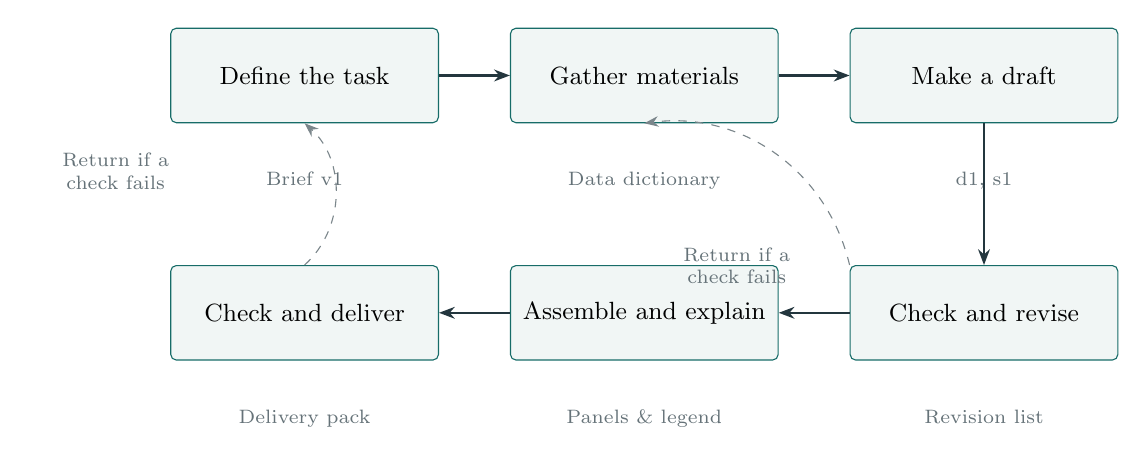
\begin{tikzpicture}[
  box/.style={draw=BookTeal,rounded corners=2pt,fill=BookPale,minimum width=34mm,minimum height=12mm,align=center,font=\small},
  link/.style={-{Stealth[length=2mm]},thick,draw=BookInk},
  loop/.style={-{Stealth[length=1.8mm]},dashed,draw=BookInk!60},
  note/.style={font=\scriptsize,text=BookInk!70,align=center}
]
\node[box] (a) {Define the task};
\node[box,right=9mm of a] (b) {Gather materials};
\node[box,right=9mm of b] (c) {Make a draft};
\node[box,below=18mm of c] (d) {Check and revise};
\node[box,left=9mm of d] (e) {Assemble and explain};
\node[box,left=9mm of e] (f) {Check and deliver};
\node[note,below=5mm of a] {Brief v1};
\node[note,below=5mm of b] {Data dictionary};
\node[note,below=5mm of c] {d1, s1};
\node[note,below=5mm of d] {Revision list};
\node[note,below=5mm of e] {Panels \& legend};
\node[note,below=5mm of f] {Delivery pack};
\draw[link] (a)--(b);
\draw[link] (b)--(c);
\draw[link] (c)--(d);
\draw[link] (d)--(e);
\draw[link] (e)--(f);
\draw[loop] (d.north west) to[bend right=42] (b.south);
\draw[loop] (f.north) to[bend right=48] (a.south);
\node[note,align=center,text width=20mm] at ($(b.south)!0.45!(d.north west)+(0,-10mm)$) {Return if a check fails};
\node[note,align=center,text width=20mm] at ($(a.south)!0.45!(f.north)+(-24mm,2mm)$) {Return if a check fails};
\end{tikzpicture}
}
\caption{The six stages used throughout this book. Stages that do not apply can be skipped; when a check fails, follow the dashed loop back to the stage where the problem originated rather than redrawing blindly in place. Grey notes underneath each box list the artifacts produced at that stage in this chapter's river-nitrate case (\texttt{d1} and \texttt{s1} denote the initial data-panel and schematic-panel drafts).}\label{fig:ch01-01}
\end{figure}

These six stages are not a one-way conveyor belt. As the dashed feedback loops in Figure~\ref{fig:ch01-01} show, whenever an inspection in ``Check and revise'' or ``Check and deliver'' reveals an error, the critical move is to \textbf{identify which upstream stage created the error and return to that stage to fix it}, rather than regenerating drafts blindly in place. Below is what happens at each stage and how work is divided among AI tools, deterministic software, and the author.

\textbf{Stage 1: Define the task.} Before opening any generation or plotting page, write down the intended venue and dimensions (which figure in which manuscript, single- or double-column width), the target readership, the one-sentence testable goal, required objects and relationships, visual constraints, explicit exclusions, and acceptance criteria. AI can help organize rough notes into brief fields and flag missing specifications; the author decides the research question, separates established facts from hypotheses, and sets the acceptance bar. Drawing briefs are covered in Chapter 2, composition and sketch planning in Chapter 3, and visual language in Chapter 4.

\textbf{Stage 2: Gather materials.} Collect raw data tables, station metadata, literature references, or original instrument images into a single source folder, check version compatibility, and write a concise data dictionary or material note. AI can help write download and parsing scripts, scan for missing values and quality codes, and draft summary tables; the author must verify physical units against official documentation (such as distinguishing $\text{mg/L as N}$ from $\text{mg/L as NO}_3^-$), confirm that only approved records rather than provisional data are used, and lock a read-only backup of the raw files.

\textbf{Stage 3: Make a draft.} Route each panel to the tool matching its material category from Section 1.2: deterministic scripts or scientific visualization for data panels (Chapter 5), workflow or mechanism generators for explanatory diagrams (Chapters 6 and 7), and non-destructive presentation tools for experimental imagery (Chapter 8). AI and plotting engines execute explicit instructions to render charts or generate text-free schematic bases; the author translates the brief into prompts or script parameters, saves every submitted instruction verbatim, and screens initial candidates.

\textbf{Stage 4: Check and revise.} Audit the draft line by line against the brief and data dictionary, checking scientific accuracy and data fidelity before fine-tuning colors or fonts, and compile defects into a structured revision list. AI executes specific revision commands; the author diagnoses the root cause of each flaw and chooses the return path. If an axis unit is incomplete or empty cells were read as zeros, follow the loop in Figure~\ref{fig:ch01-01} back to ``Gather materials''; if a drinking-water standard was labeled as an in-stream exceedance, return to ``Define the task'' to clarify the conceptual boundary. After every edit, the author re-verifies the entire figure, checking that unchanged elements remained intact. Chapter 11 details layered revision strategies.

\textbf{Stage 5: Assemble and explain.} For multi-panel figures, establish grid proportions, reading order, and panel letters (\textbf{a}, \textbf{b}, \dots), overlay vector labels onto schematic bases, and write a figure legend matching the visual evidence. Multi-panel tools (\sdtool{multi-panel-figure-maker}) handle grid layout, lettering, and journal width presets, while legend assistants (\sdtool{figure-legend}) can draft an initial outline from the image; the author must supply context invisible in the pixels (station ID, download date, conversion factors, missing-data handling, reference-line scope) and remove unsupported speculation. Multi-panel assembly and legends are covered in Chapter 9, graphical abstracts in Chapter 10, and posters and slides in Chapter 12.

\textbf{Stage 6: Check and deliver.} Inspect the figure at 100\% of its print width (such as $174\ \text{mm}$ for a double-column figure) to verify font sizes, line weights, resolution, and color-vision accessibility, then package the source files, brief, drafts, final exports, legends, and AI-use log into an archive. Checking tools (\sdtool{figure-checker}) detect technical issues in resolution, color mode, and contrast; the author performs final scientific verification and checks journal policy compliance. Chapter 13 covers verification and delivery standards.

\section{One figure from brief to final: river nitrate}

We now walk through all six stages using Lin's agricultural river nitrate figure.

The study area is the Raccoon River watershed in west-central Iowa, USA, an intensively farmed basin dominated by corn--soybean rotation with widespread subsurface tile drainage. Previous studies in this watershed have shown that precipitation infiltrating through agricultural soils into tile drains and baseflow provides the main pathway delivering nitrate-nitrogen to the river network (Schilling and Zhang, 2004), while in-situ ultraviolet nitrate sensors allow continuous daily tracking of river nitrate concentrations across flow regimes (Pellerin et al., 2016).

Lin retrieves the full-year 2016 approved daily record from the USGS National Water Information System (NWIS) for the downstream gauge at Van Meter, Iowa (station 05484500). Here she sets an explicit scientific boundary: \textbf{this figure shows only the temporal covariation of nitrate concentration and stream discharge at station 05484500 during 2016, alongside a simplified schematic of the transport pathway from tile-drained cropland to the gauge; it does not perform quantitative source apportionment, calculate nitrogen loads, or make causal or statistical significance claims.} The U.S. Environmental Protection Agency (EPA) Maximum Contaminant Level (MCL) of $10\ \text{mg/L}$ (as N) applies legally to finished public drinking water rather than untreated river water, and is shown strictly as a numerical reference line.

\textbf{Stage 1: Define the task---writing a verifiable drawing brief.} Learning from her initial false start, Lin expands her goal into a structured drawing brief and saves it as a text file in her project folder; later, after picking a route in the \scidraw{} figure workflow guide (\sdtool{figure-workflow}), she pastes it into the tool at each step. Below are the core fields (the complete version is in the \texttt{cases/} directory of the book repository):

\begin{Prompt}
[Use and audience] Environmental science paper Figure 2, double-column width 174 mm,
height ~110 mm; audience is hydrology and water-quality peers.
[Goal] Understand the 2016 seasonal variation of nitrate concentration in the Raccoon
River and its temporal covariation with discharge, and locate daily means, missing days,
the 10 mg/L (as N) reference line, and winter ice-affected estimated discharge periods.
[Materials] (1) USGS station 05484500 approved 2016 daily means (nitrate in mg/L as N;
discharge in ft3/s); (2) published site description of cropland subsurface tile drainage
entering the river network (Schilling & Zhang 2004).
[Objects and relationships] Panel a (left, ~36% width): cropland -> subsurface tile drains
-> tributary ditch -> main river channel -> monitoring station. Panel b (right, ~62% width):
two vertically stacked subplots sharing a monthly time axis (top: nitrate; bottom: discharge).
[Visual style] White background; single colorblind-safe hue per data subplot; flat 2D
low-saturation schematic base with zero embedded text.
[Limits] No smoothing, interpolation, or point deletion; break curves at missing days;
convert discharge to m3/s on a log scale; label 10 mg/L line as reference only, never
"exceeds limit"; exclude factories, outfalls, dead fish, or algal blooms from panel a.
[Acceptance] All 363 nitrate and 366 discharge daily values plotted; 3 gap breaks visible;
extrema (13.9 on May 13; 3.19 on Sep 16) verifiable; all text >= 6 pt at 174 mm width.
\end{Prompt}

This brief turns design choices into a clear logical chain: because `[Goal]` requires comparing daily concentration and flow while `[Materials]` shows that the two quantities differ in units and span different orders of magnitude, `[Objects and relationships]` specifies two vertically stacked subplots sharing a monthly axis and rules out twin Y axes. Because `[Materials]` includes only single-station sensor records and tile-drainage literature, `[Limits]` forbids factories, outfalls, or dead fish, and `[Acceptance]` locks in the exact observation counts (363 and 366) and extreme dates (May 13 and September 16).

\textbf{Stage 2: Gather materials---the data dictionary and three common traps.} In the second stage, Lin uses a script to download the 2016 daily file for station 05484500 from the USGS NWIS daily service (parameter \texttt{99133} for in-situ nitrate plus nitrite in $\text{mg/L as N}$, parameter \texttt{00060} for discharge in $\text{ft}^3/\text{s}$, statistic code \texttt{00003} for daily mean; public domain, DOI \texttt{10.5066/F7P55KJN}) and parses it into \path{raccoon-2016-daily.csv}. Eight representative rows illustrate the structure:

\begin{Prompt}
date,nitrate_mgL_as_N,nitrate_qual,discharge_cfs,discharge_qual
2016-01-01,12.1,A,6610,A
2016-01-08,11.1,A,4990,A:e
2016-05-01,8.66,A,16300,A
2016-05-13,13.9,A,10200,A
2016-09-16,3.19,A,5500,A
2016-09-18,,,7110,A
2016-09-19,,,8180,A
2016-12-14,,,968,A:e
\end{Prompt}

She also compiles a data dictionary with full-table verification values:

\begin{center}\footnotesize
\setlength{\tabcolsep}{3pt}
\renewcommand{\arraystretch}{1.15}
\begin{tabularx}{\linewidth}{@{}l>{\raggedright\arraybackslash}p{25mm}>{\raggedright\arraybackslash}p{27mm}Y@{}}
\toprule
\textbf{Column name} & \textbf{Physical meaning} & \textbf{Units and codes} & \textbf{2016 full-table verification values} \\
\midrule
\texttt{date} & Calendar date & \texttt{YYYY-MM-DD} & 366 rows in total (2016 is a leap year) \\
\texttt{nitrate\_mgL\_as\_N} & Daily mean in-situ nitrate plus nitrite & $\text{mg/L}$ (as N); empty cell indicates missing day & 363 valid days; 3 missing days (Sep 18--19, Dec 14); max $13.9$ (May 13), min $3.19$ (Sep 16); 162 days $>10\ \text{mg/L}$; highest monthly mean in May ($12.84$), lowest in Sep ($5.36$), with Jan also high ($11.75$) \\
\texttt{nitrate\_qual} & Nitrate quality flag & \texttt{A} = Approved by USGS & All 363 valid rows flagged \texttt{A}; no provisional data \\
\texttt{discharge\_cfs} & Daily mean stream discharge & $\text{ft}^3/\text{s}$; multiply by $0.028316846592$ to convert to $\text{m}^3/\text{s}$ & All 366 days valid; max $16,300\ \text{ft}^3/\text{s}$ ($\approx 461.6\ \text{m}^3/\text{s}$, May 1), min $411\ \text{ft}^3/\text{s}$ ($\approx 11.6\ \text{m}^3/\text{s}$, Sep 6) \\
\texttt{discharge\_qual} & Discharge quality flag & \texttt{A} = Approved; \texttt{A:e} = Approved, ice-affected estimate & 58 days flagged \texttt{A:e}, concentrated in Jan--Feb and Dec \\
\bottomrule
\end{tabularx}
\end{center}

This table highlights three traps that must be resolved during material preparation:

First, \textbf{``as N'' versus ``as $\text{NO}_3^-$'' differs by a factor of 4.43.} Nitrate concentration can be reported either by nitrogen atomic mass ($\text{mg/L as N}$, molar mass $14.01\ \text{g/mol}$) or by whole nitrate ion mass ($\text{mg/L as NO}_3^-$, molar mass $62.00\ \text{g/mol}$); for the same water sample, the latter is $62.00 / 14.01 \approx 4.43$ times larger. Both USGS parameter \texttt{99133} and the EPA $10\ \text{mg/L}$ standard use ``as N.'' Omitting ``as N'' from the axis label will cause peers accustomed to whole-ion reporting to misread the concentrations by more than fourfold.

Second, \textbf{discharge unit conversion and dynamic range affect interpretation.} Raw USGS discharge is in $\text{ft}^3/\text{s}$, whereas international journals generally require $\text{m}^3/\text{s}$. Converting units shifts all plotted numbers (from $411\text{--}16,300$ to $11.6\text{--}461.6$), and because peak flow is nearly 40 times baseflow, a logarithmic axis is needed to show both regimes clearly. Both transformations must be documented in the archive and legend.

Third, \textbf{missing days and ice-affected estimates must be preserved.} In 2016, three days of nitrate data are missing and 58 winter discharge values are flagged \texttt{A:e} (ice-affected estimates). Dropping rows with empty cells would delete valid discharge records for those three days and cause the line plot to bridge the gap seamlessly; ignoring the quality column would hide which winter flows are estimates. The parser must therefore keep all 366 rows, leave missing values empty, and pass \texttt{A:e} flags to the plotting script.

Here, AI can write the parsing script and tally missing values or quality codes, but checking the parameter manual to confirm ``as N,'' verifying that no provisional data are mixed in, and recording the download date must be done by the author.

\textbf{Stage 3: Make a draft---contrasting vague and brief-driven data plots.} To see the difference a brief makes, first consider the output of a vague one-sentence request:

\begin{Prompt}
Help me turn these river data into a professional paper figure that highlights the nitrate pollution problem.
\end{Prompt}

Without explicit constraints, default scripts or automated visualization tools frequently produce problem drafts like Figure~\ref{fig:ch01-03}.

\begin{figure}[htbp]\centering
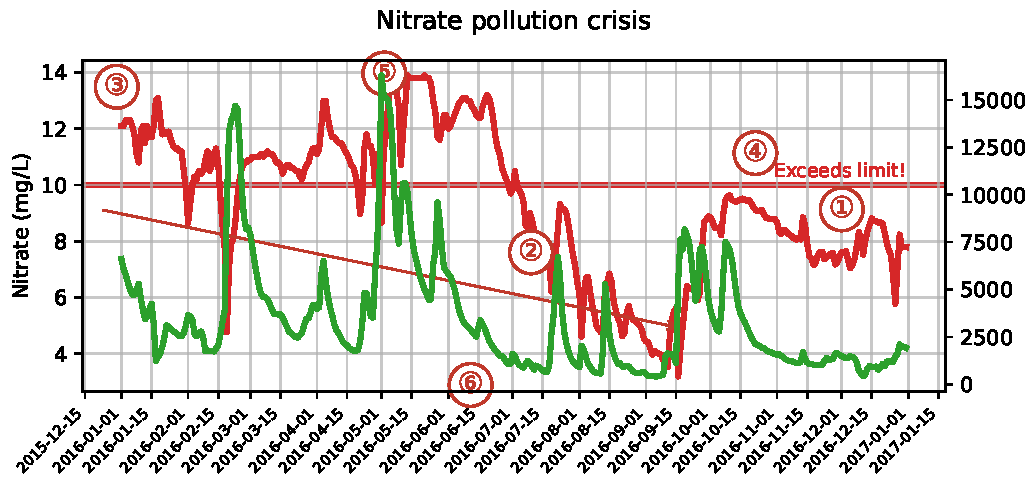
\includegraphics[width=\linewidth]{figures/ch01/ch01-03-nitrate-draft-vague-en.pdf}
\caption{Typical data-plot defects under a vague request (constructed from the real USGS daily record as a counterexample). Here (1) twin axes with red--green coloring, (2) straight lines bridging missing days, (3) incomplete units, (4) a drinking-water reference line labeled ``Exceeds limit!'', (5) a conclusion-laden title, and (6) crowded date ticks all invite misreading.}\label{fig:ch01-03}
\end{figure}

Checking Figure~\ref{fig:ch01-03} against the brief reveals six clear defects marked by red circles: (1) Red--green twin Y axes with unconverted $\text{ft}^3/\text{s}$ discharge create arbitrary curve intersections that falsely suggest concentration and flow are ``equal,'' while clashing for color-vision-deficient readers; (2) the missing days on September 18--19 and December 14 (indicated by thin arrows) are bridged by straight lines, fabricating three days of observations; (3) the left axis omits ``as N'' and the right axis lacks units or any distinction for winter ice estimates; (4) $y=10$ is drawn as a bold red line labeled ``Exceeds limit!'', misapplying a drinking-water standard to untreated river water; (5) the title ``Nitrate pollution crisis'' imposes a conclusion on the reader; and (6) biweekly full-date labels crowd the horizontal axis over a heavy grid.

Now consider the brief-driven workflow. After uploading \path{raccoon-2016-daily.csv} to \scidraw{} scientific visualization (\sdtool{sci-vis}), Lin submits a structured instruction:

\begin{Prompt}
Read the uploaded raccoon-2016-daily.csv. date is calendar date; nitrate_mgL_as_N is
daily mean nitrate plus nitrite (mg/L as N); discharge_cfs is daily mean flow (ft3/s).
Plot two vertically stacked subplots sharing the horizontal time axis (no twin Y axes):
Top subplot: line plot of daily nitrate; y-axis "Nitrate (mg/L as N)"; draw a dashed
gray horizontal line at 10 labeled "US EPA drinking-water MCL (reference only)".
Bottom subplot: convert discharge to m3/s (multiply by 0.028316846592) on a log scale;
y-axis "Discharge (m3/s, log scale)"; highlight dates where discharge_qual is A:e
with a lighter wide band and legend "Light: ice-affected estimates".
Leave missing nitrate dates as visible line breaks; do not interpolate, smooth, or drop rows.
Format x-axis with monthly ticks Jan-Dec 2016. Use one colorblind-safe color per panel.
Omit figure titles and evaluative labels such as "exceeds limit" or "crisis".
\end{Prompt}

Executing deterministic plotting under these rules yields the revised data panel (Figure~\ref{fig:ch01-04}).

\begin{figure}[htbp]\centering
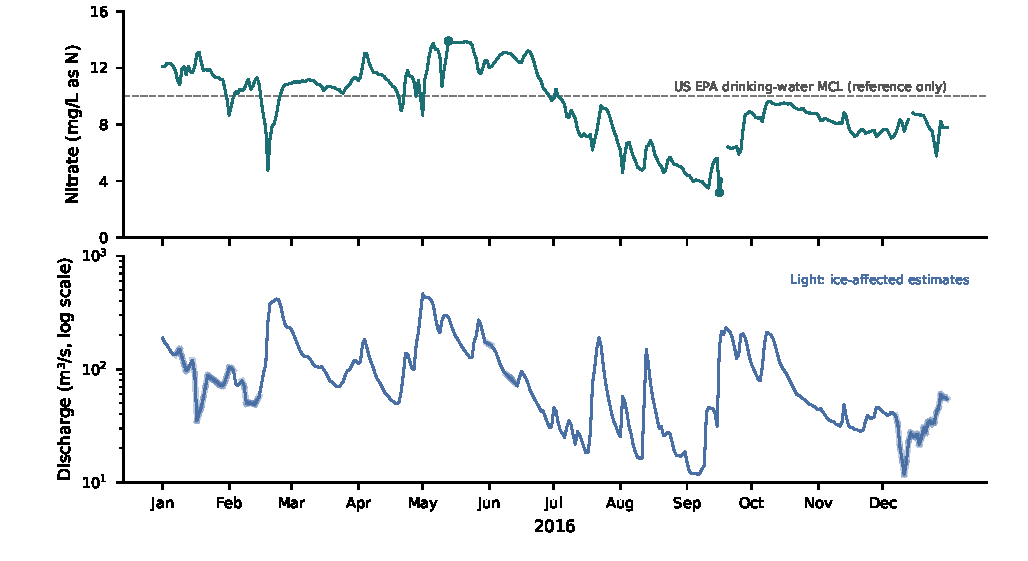
\includegraphics[width=\linewidth]{figures/ch01/ch01-04-nitrate-panel-brief-en.pdf}
\caption{The same dataset replotted from the brief. Top: daily mean nitrate plus nitrite ($\text{mg/L as N}$), with line breaks at the missing days (September 18--19 and December 14); the dashed grey line marks the US EPA drinking-water Maximum Contaminant Level of $10\ \text{mg/L as N}$, shown for reference only because it does not apply to untreated river water. Bottom: daily mean discharge converted from $\text{ft}^3/\text{s}$ to $\text{m}^3/\text{s}$ on a logarithmic scale; lighter segments indicate winter ice-affected estimates. Data: USGS station 05484500, Raccoon River at Van Meter, Iowa, approved daily values downloaded October 29, 2026.}\label{fig:ch01-04}
\end{figure}

Comparing Figure~\ref{fig:ch01-04} with Figure~\ref{fig:ch01-03}, all six defects are resolved: stacked subplots sharing a monthly axis eliminate false curve crossings and allow direct vertical comparison of flow pulses and nitrate responses; the top curve breaks cleanly at the three missing dates and marks the annual maximum ($13.9\ \text{mg/L}$ on May 13) and minimum ($3.19\ \text{mg/L}$ on September 16); the $10\ \text{mg/L}$ line is a muted gray dashed reference; and the bottom panel uses a logarithmic $\text{m}^3/\text{s}$ scale with a lighter band marking the 58 ice-affected days. The unsmoothed plot also preserves an important empirical fact: although monthly mean nitrate was highest in May ($12.84\ \text{mg/L}$) and lowest in September ($5.36\ \text{mg/L}$), January concentrations were also high ($11.75\ \text{mg/L}$). Avoiding smoothing and biased titles lets the true seasonal record stand on its own.

\textbf{Stage 3 (continued): Make a draft---contrasting vague and brief-driven study-area schematics.} Next, we build panel a, the study-area schematic. First consider what happens when an image generator receives only a broad one-line prompt:

\begin{Prompt}
Illustration of nitrate pollution in an agricultural river watershed. Aspect ratio 4:3.
\end{Prompt}

Many people assume that vague prompts mainly risk garbled pseudo-text or smoking factory chimneys. When we generated three images from this exact prompt, the results taught a more important lesson: none of the three runs produced factory smokestacks or dead fish, and the English labels and arrows were largely readable; yet to illustrate ``pollution,'' the model invented \textbf{facilities and ecological mechanisms unsupported by our case materials}. Figure~\ref{fig:ch01-05} shows a representative output, with red circles 1--4 marking four specific problems.

\begin{figure}[htbp]\centering
\begin{tikzpicture}
\node[anchor=south west,inner sep=0] (img) at (0,0) {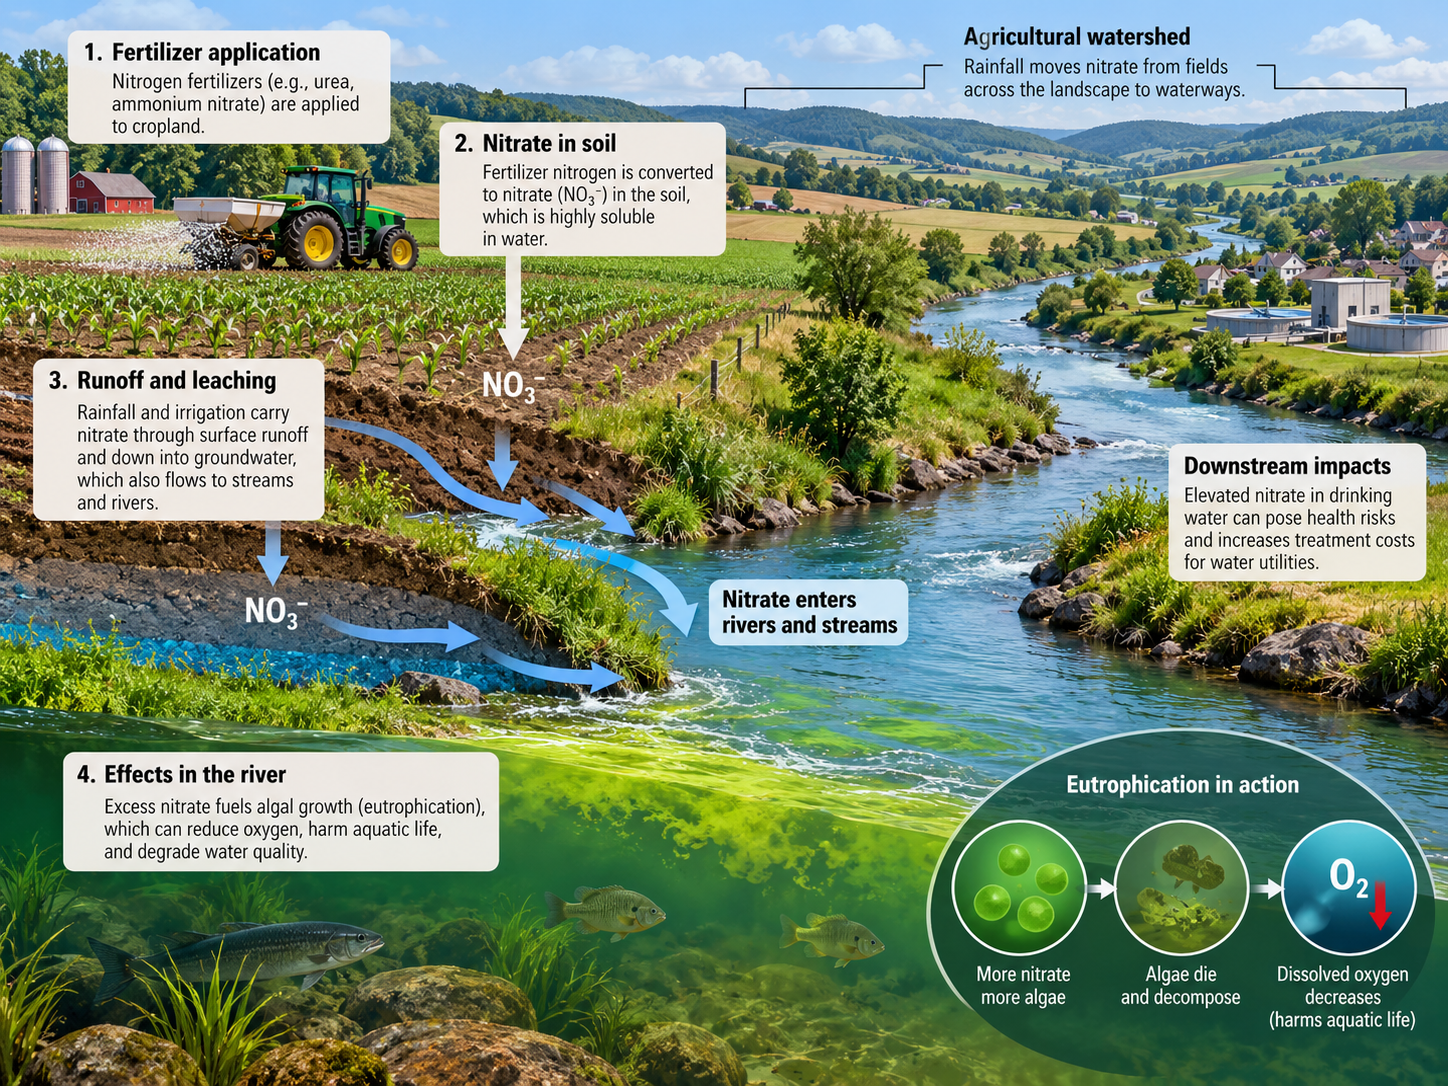
\includegraphics[width=\linewidth]{figures/ch01/ch01-05-site-schematic-vague.png}};
\begin{scope}[x={(img.south east)},y={(img.north west)}]
  \tikzset{badmark/.style={draw=red!80!black,very thick,circle,fill=white,fill opacity=0.88,text opacity=1,text=red!80!black,font=\bfseries\small,inner sep=1.2pt}}
  \node[badmark] at (0.88,0.72) {1};
  \node[badmark] at (0.80,0.22) {2};
  \node[badmark] at (0.22,0.80) {3};
  \node[badmark] at (0.62,0.45) {4};
\end{scope}
\end{tikzpicture}
\caption{A study-area schematic generated from a one-line prompt (the example images in this chapter were generated by an image model; prompts and generation logs are available in the book repository). Without generating factory chimneys or gibberish text, the model still added content unsupported by our case materials: (1) a water-treatment complex with circular tanks, town buildings, and utility-cost claims on the right bank; (2) foreground algal blooms, underwater fish, and a lower-right ``eutrophication---algal decomposition---dissolved oxygen depletion'' diagram (while omitting subsurface tile drains from the left soil cut-away); (3) photorealistic landscape and underwater views with large English text boxes baked into the bitmap; and (4) runoff arrows without the downstream USGS monitoring station or sensor.}\label{fig:ch01-05}
\end{figure}

Examining these four defects one by one shows why the image fails scientific review:
\begin{itemize}
\item \textbf{Problem (1) (Unsupported water-treatment plant and cost claims):} On the right bank (circle 1), the model drew a town and a water-treatment facility with two circular basins, alongside text discussing drinking-water risks and utility treatment costs. Our dataset contains no water-plant locations or cost records; including them misleads readers about the scope of the paper.
\item \textbf{Problem (2) (Unmeasured eutrophication mechanism and omitted tile drains):} The foreground and lower-right inset (circle 2) depict dense green algal blooms, fish, and a causal diagram ($\text{nitrate increase} \rightarrow \text{algal decomposition} \rightarrow \text{dissolved oxygen } [\text{O}_2] \text{ drop}$), whereas the soil cut-away on the left shows only surface runoff and groundwater, omitting the subsurface tile drains central to this watershed. Presenting unmeasured downstream ecological effects as fact while leaving out the primary transport pathway is a serious scientific distortion.
\item \textbf{Problem (3) (Photorealistic decoration and text locked in bitmap pixels):} The scene (circle 3) uses realistic skies, a distant tractor, and underwater lighting, with four large English text blocks rasterized directly into the bitmap where their font size, style, and wording cannot be edited separately.
\item \textbf{Problem (4) (Missing monitoring station location):} Although runoff arrows are present, the downstream channel (circle 4) lacks the USGS 05484500 monitoring station and in-situ sensor needed to link panel a to the data in panel b.
\end{itemize}

Keeping a schematic faithful to the science requires two rules: first, specify \textbf{required scientific objects} alongside a \textbf{strict exclusion list}; second, require a \textbf{clean base image with zero embedded text}, adding vector labels later in a layout or typesetting tool. Below is the core portion of the structured prompt (the full prompt is in the \texttt{cases/} directory of the book repository):

\begin{Prompt}
Flat 2D scientific schematic for a journal figure panel, portrait 4:5, pure white
background. Clean vector style: flat fills, thin dark-gray outlines, no gradients,
no shadows, no 3D, no texture.
ABSOLUTELY NO TEXT: no letters, words, numbers, symbols, labels, legend, or title.
SCENE: simplified oblique (~30-degree) view of an agricultural landscape with a
cut-away soil block in the lower-left quarter.
- Upper half: 5-6 rectangular fields in muted sage green and wheat yellow; no buildings.
- Meandering river (soft blue) from upper-left to lower-right, joined by one tributary ditch.
- Lower-left soil cut-away: 3 round gray subsurface drain pipes, one outlet discharging
  into the tributary ditch.
- Lower-right river bank: simple gray monitoring station box with cable to a submerged
  cylindrical sensor; 2-3 hollow chevrons on water surface pointing downstream.
STRICTLY EXCLUDE: factories, chimneys, sewage pipes, towns, bridges, dead fish, algae,
murky water, warning signs, chemical symbols, clouds, decorative borders.
\end{Prompt}

Even with a detailed prompt, every candidate output must be inspected against the brief. We generated three images from this prompt and found distinct differences: in the first run, a white gap broke the connection between the receiving channel beside the soil cut-away and the tributary ditch joining the main river, severing the ``tile drain $\rightarrow$ ditch $\rightarrow$ river'' pathway, so it was rejected; in the third run, two separate tributary ditches entered the main channel independently, departing from our single-ditch design, so it too was rejected; only the second run delivered a white background, zero text, six cropland fields, three gray drain-pipe cross-sections, a continuous tributary ditch entering the main river, the downstream monitoring box and sensor, and three white downstream V-chevrons, with no excluded objects.

Zooming in to 200\% on that second image still reveals four minor deviations: the ditch forms a small Y-junction before entering the river; the third drain pipe on the right doubles directly as the flowing outlet; the sensor rests at the water surface with ripples rather than appearing deeply submerged; and the soil block and station box retain subtle grain texture and shading. Because none of these details alter the core topological pathway---cropland to subsurface tile drains to ditch to main channel to gauge---and the image is free of pseudo-text, we can note ``Schematic, not to scale'' in the legend and overlay six vector labels in LaTeX to obtain a sound study-area panel (Figure~\ref{fig:ch01-06}).

\begin{figure}[htbp]\centering
\begin{tikzpicture}
\node[anchor=south west,inner sep=0] (img) at (0,0) {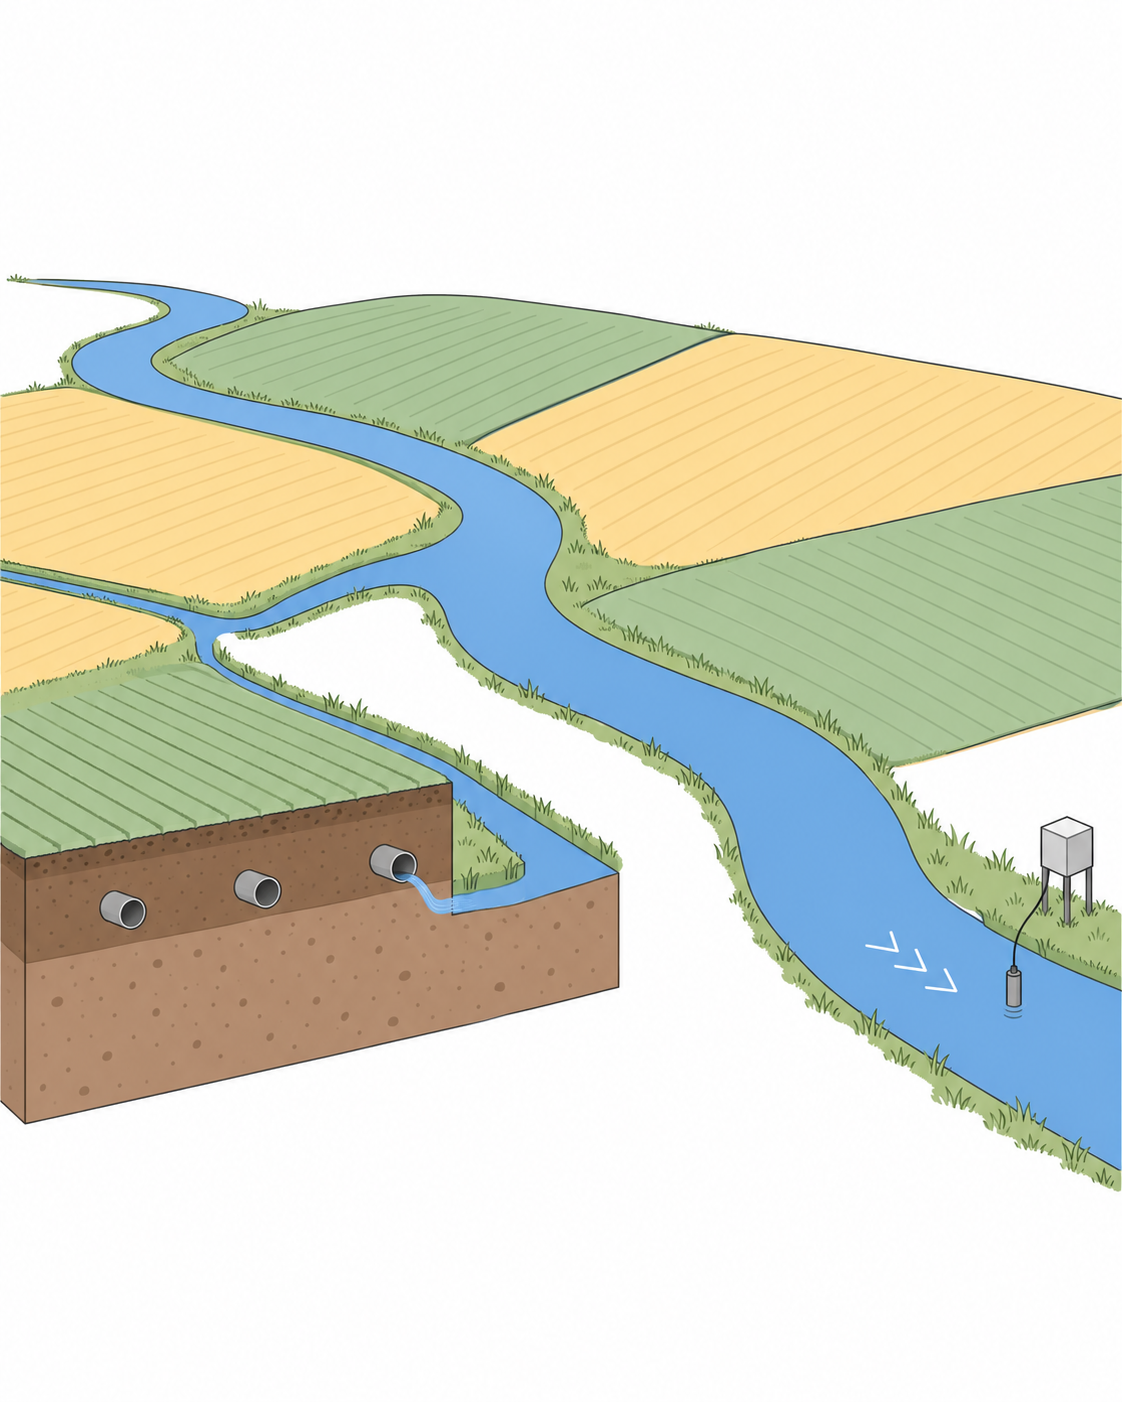
\includegraphics[width=0.62\linewidth]{figures/ch01/ch01-06-site-schematic-brief.png}};
\begin{scope}[x={(img.south east)},y={(img.north west)}]
  \tikzset{lbl/.style={font=\footnotesize,fill=white,fill opacity=0.82,text opacity=1,inner sep=1.5pt,align=center}}
  \node[lbl] at (0.50,0.88) {Cropland (corn--soybean, schematic)};
  \node[lbl] at (0.22,0.18) {Subsurface tile drains};
  \node[lbl] at (0.12,0.45) {Drainage ditch};
  \node[lbl] at (0.55,0.55) {Raccoon River};
  \node[lbl] at (0.80,0.12) {USGS 05484500 station};
  \node[lbl] at (0.72,0.36) {Flow};
\end{scope}
\end{tikzpicture}
\caption{The study-area schematic base generated from the brief (the second of three runs) with English labels overlaid afterward. The base image contains no generated text, excludes unrelated facilities and unverified ecological effects, and clearly shows the spatial pathway from cropland and subsurface tile drains through the drainage ditch into the Raccoon River and down to the monitoring station.}\label{fig:ch01-06}
\end{figure}

\textbf{Stage 4: Check and revise---managing iterations with a revision list.} Instead of asking a tool to ``make it look more professional,'' compare the data draft (Figure~\ref{fig:ch01-03}) and schematic draft (Figure~\ref{fig:ch01-05}) against the brief and log every problem in a structured \textbf{revision list} specifying the verifiable fix and the stage to return to:

\begin{center}\footnotesize
\setlength{\tabcolsep}{3pt}
\renewcommand{\arraystretch}{1.15}
\begin{tabularx}{\linewidth}{@{}c>{\raggedright\arraybackslash}p{32mm}>{\raggedright\arraybackslash}p{22mm}Y>{\raggedright\arraybackslash}p{22mm}@{}}
\toprule
\textbf{\#} & \textbf{Defect found in draft} & \textbf{Clause violated} & \textbf{Verifiable revision instruction} & \textbf{Stage to return to} \\
\midrule
1 & Twin Y axes make curve crossings look like ``equal concentration and flow'' & [Objects and relationships] & Split into two vertically stacked subplots sharing the horizontal time axis & Make a draft \\
2 & Missing days (Sep 18--19, Dec 14) bridged by straight lines & [Limits], [Acceptance] & Keep empty cells as \texttt{NaN} so the curve breaks naturally at all three gaps without interpolation & Gather materials (check parser logic) \\
3 & Axis label omits ``as N''; discharge lacks units and conversion & [Materials], [Limits] & Write full units; multiply discharge by $0.028316846592$ to $\text{m}^3/\text{s}$ on a log axis & Gather materials \\
4 & $10\ \text{mg/L}$ line labeled ``Exceeds limit!''; conclusion-laden title at top & [Limits] & Remove title; change to dashed gray line labeled ``drinking-water MCL (reference only)'' & Define the task (clarify scope) \\
5 & High-saturation red--green palette; crowded biweekly date strings & [Visual style] & Use one colorblind-safe hue per subplot; use monthly ticks Jan--Dec & Make a draft \\
6 & Winter 58 days of ice-affected estimated flow (\texttt{A:e}) indistinguishable from measured flow & [Goal] & Highlight \texttt{A:e} dates with a lighter wide line and add a subplot legend & Make a draft \\
7 & Schematic draft adds water plant, algal bloom, and eutrophication inset while omitting tile drains & [Objects and relationships], [Limits] & Do not patch locally; regenerate a text-free base from the brief's object and exclusion lists & Make a draft \\
8 & Schematic text baked into bitmap, with broken ditch in run 1 and two ditches in run 3 & [Visual style], [Objects and relationships] & Forbid text in base image; select run 2 with continuous ditch path and overlay vector labels & Check and revise \\
\bottomrule
\end{tabularx}
\end{center}

Keep one iron rule in mind: \textbf{after every revision, re-verify the entire figure from scratch, including parts you did not ask to change.} Generative redrawing can fix a drainage ditch while dropping the monitoring station, and adjusting axis padding in a script can clip the annual peak. Three habits keep re-verification reliable: first, place the old and new versions side by side (or flip rapidly between them) to spot unintended drift in unchanged areas; second, check the extreme dates and gap dates from the data dictionary directly on the plot to confirm that peaks, troughs, and breaks sit at the exact dates; third, zoom to 200\% to recount key scientific objects and connection directions against the acceptance checklist.

\textbf{Stages 5 and 6: Assemble and explain, final-size inspection, and delivery.} Once both panels pass verification, move to Stage 5, ``Assemble and explain.'' In \scidraw{}, download the schematic and data panels to your local folder, open the multi-panel assembly tool (\sdtool{multi-panel-figure-maker}), select a $1 \times 2$ grid with an approximate $36:62$ width ratio between left panel \textbf{a} and right panel \textbf{b}, apply automatic bold lettering \textbf{a}/\textbf{b} and the $174\ \text{mm}$ double-column journal width preset, and export a ZIP package containing TIFF, PNG, PDF, PPTX, and processing records. Aligning the two panels produces the complete Figure 2 (Figure~\ref{fig:ch01-07}).

\begin{figure}[htbp]\centering
{\makeatletter\tikzset{text width/.code={\def\tikz@text@width{#1\textwidth}}}\makeatother\begin{tikzpicture}
\node[anchor=south west,inner sep=0] (panel) at (0,0) {%
  \begin{minipage}[t]{0.34\linewidth}
    \IfFileExists{figures/ch01/ch01-06-site-schematic-brief.png}{%
      \begin{tikzpicture}
      \node[anchor=south west,inner sep=0] (img) at (0,0) {%
        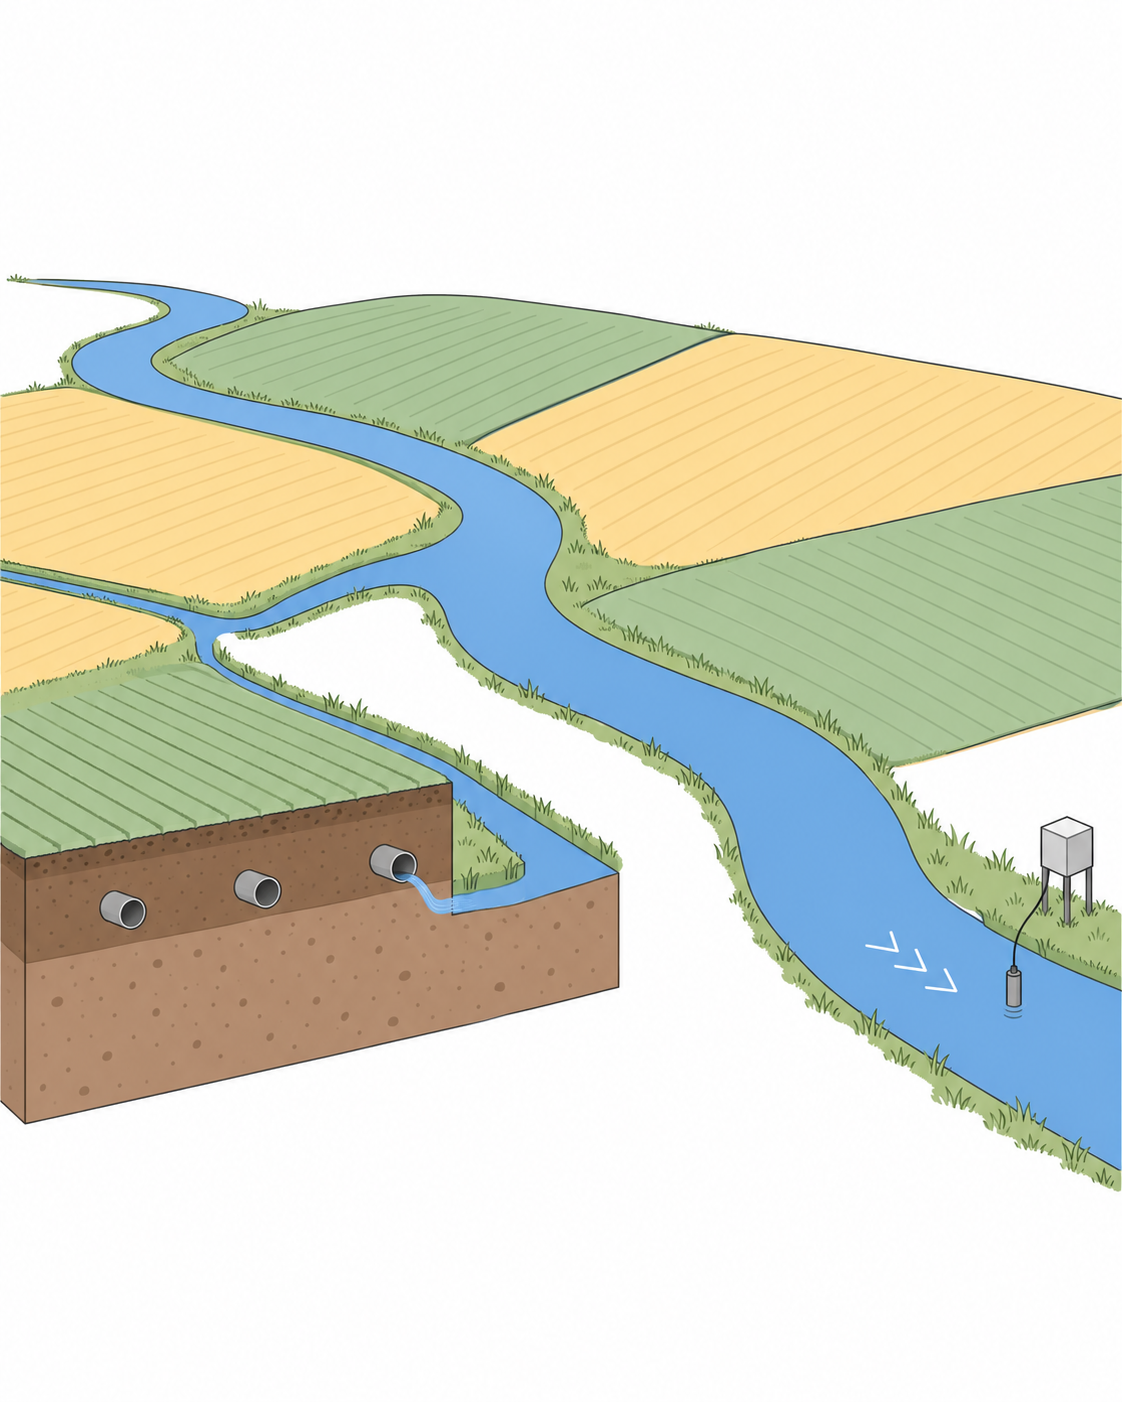
\includegraphics[width=\linewidth]{figures/ch01/ch01-06-site-schematic-brief.png}};
      \begin{scope}[x={(img.south east)},y={(img.north west)}]
        \tikzset{lbl/.style={font=\scriptsize,fill=white,fill opacity=0.8,text opacity=1,inner sep=1pt,align=center}}
        \node[lbl,text width=0.28,align=center] at (0.48,0.86) {Cropland (corn--soybean, schematic)};
        \node[lbl,text width=0.22,align=center] at (0.20,0.16) {Subsurface tile drains};
        \node[lbl,text width=0.18,align=center] at (0.10,0.44) {Drainage ditch};
        \node[lbl,text width=0.22,align=center] at (0.52,0.52) {Raccoon River};
        \node[lbl,text width=0.26,align=center] at (0.52,0.10) {USGS 05484500 station};
        \node[lbl] at (0.50,0.38) {Flow};
      \end{scope}
      \end{tikzpicture}
    }{%
      \fbox{\parbox[c][0.36\linewidth][c]{0.34\linewidth}{\centering\scriptsize Missing ch01-06 base\\(codex-image; out of scope)}}
    }
    \par\vspace{1mm}{\scriptsize Schematic, not to scale}
  \end{minipage}\hfill
  \begin{minipage}[t]{0.64\linewidth}
    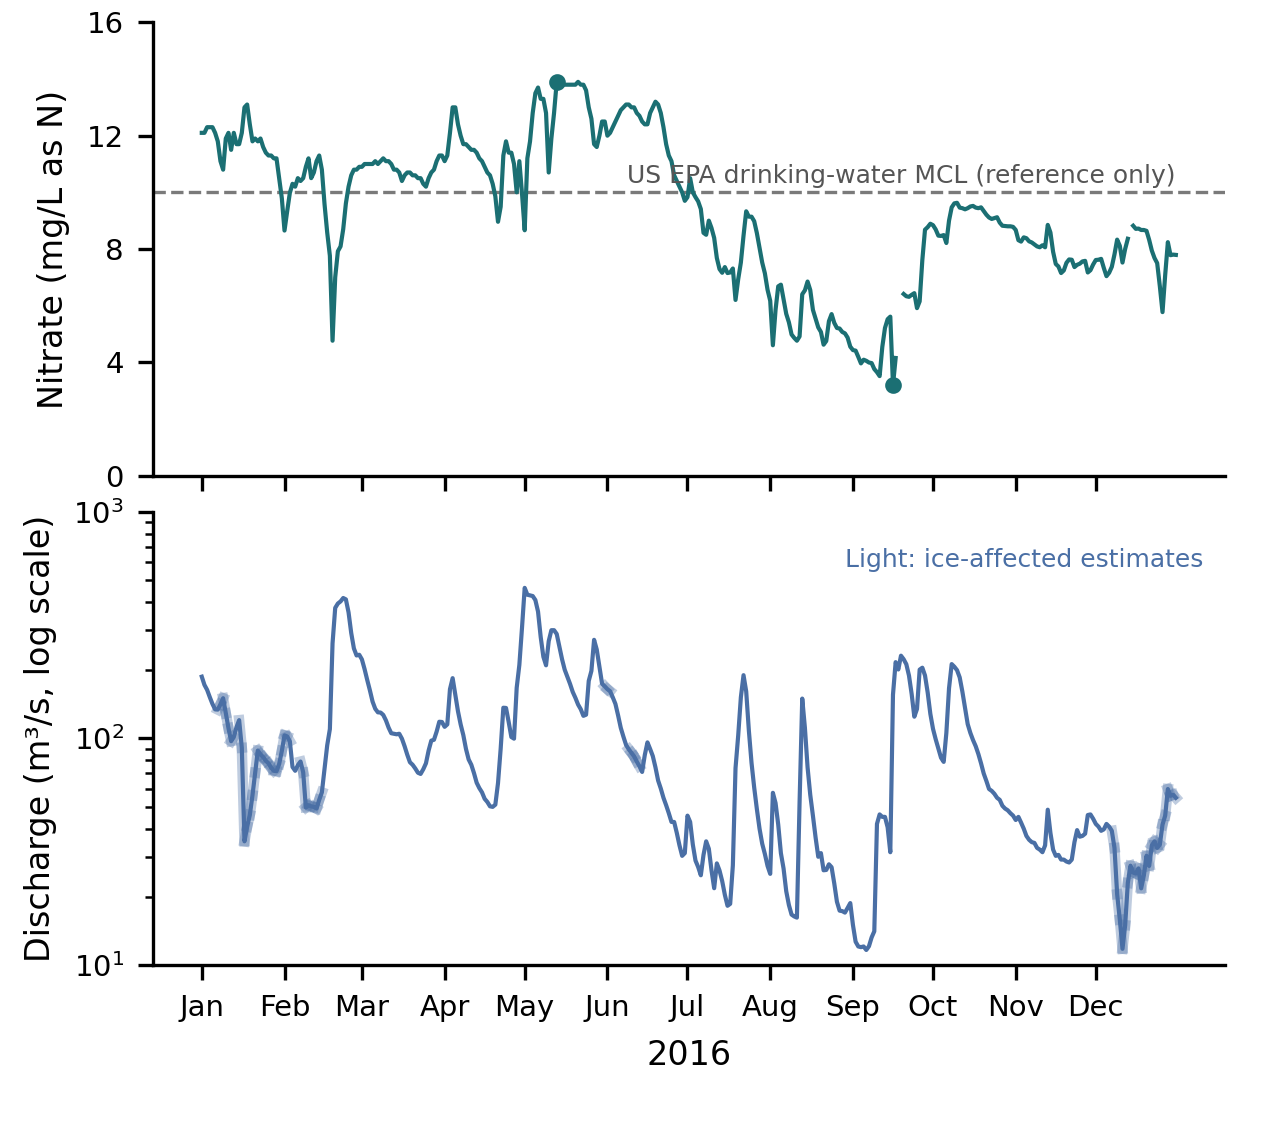
\includegraphics[width=\linewidth]{figures/ch01/ch01-04-nitrate-panel-brief-en-panel.png}
  \end{minipage}};
\node[anchor=south west,font=\bfseries\small] at ([xshift=1mm,yshift=1mm]panel.north west) {a};
\node[anchor=south west,font=\bfseries\small] at ([xshift=0.34\linewidth,yshift=1mm]panel.north west) {b};
\end{tikzpicture}
}
\caption{\textbf{Example Figure 2: nitrate concentration and discharge in the Raccoon River, 2016.} (a) Simplified study-area schematic: subsurface tile drainage from cropland enters the river channel via a ditch, with the USGS monitoring station (05484500, Van Meter, IA) downstream; not to scale, and does not represent specific fields, pipe networks, or pollution sources. (b) Top: daily mean nitrate plus nitrite ($\text{mg/L as N}$), with breaks at missing days; the dashed grey line marks the US EPA drinking-water Maximum Contaminant Level of $10\ \text{mg/L}$ (as N), for reference only. Bottom: daily mean discharge ($\text{m}^3/\text{s}$, converted from $\text{ft}^3/\text{s}$, logarithmic scale), with lighter segments indicating winter ice-affected estimates. Data are USGS approved daily values (public domain), downloaded October 29, 2026; no load calculation or statistical test is included. The schematic base was generated by an image model and labels were overlaid by the author; prompts and generation logs for this chapter's example figures are available in the book repository.}\label{fig:ch01-07}
\end{figure}

Next, write the figure legend. When uploading the final figure to the legend assistant (\sdtool{figure-legend}) to draft an outline, remember that \textbf{the model sees only image pixels and cannot know station numbers, download dates, conversion formulas, or regulatory boundaries.} The author must personally verify and add four things: (1) station ID 05484500, location, approved status, and download date; (2) ``as N'' units, gap breaks, $\text{m}^3/\text{s}$ log scaling, and the meaning of ice-affected segments; (3) statements that panel a is ``not to scale, and does not represent specific fields, pipe networks, or pollution sources,'' that the $10\ \text{mg/L}$ line is ``for reference only,'' and that ``no load calculation or statistical test is included'' (never fabricating sample sizes or test statistics); and (4) disclosure that the schematic base was made with a generative tool and labeled by the author.

Finally, in Stage 6 (``Check and deliver''), inspect the figure at 100\% of its $174\ \text{mm}$ print width to confirm that all text is $\ge 6\ \text{pt}$ and no overlaid labels obscure the drain pipes or monitoring station. Then run the technical checker (\sdtool{figure-checker}) to test resolution, color space, grayscale contrast, and color-vision accessibility. Remember that \textbf{passing a technical check does not mean the science is correct}; always verify every data point, break, and legend claim against the `[Acceptance]` criteria before archiving.

\section{Choosing a route in SciDraw AI}

The figure workflow guide (\sdtool{figure-workflow}) in \scidraw{} first asks which kind of figure you are making: \textbf{Mechanism \& workflow diagram, Data figure, Multi-panel figure, or Graphical abstract} (Figure~\ref{fig:ch01-08}). Once you pick one, the page shows a short ordered route of three or four steps, each with a one-sentence description and a button that opens the matching tool. The mechanism route, for example, runs: Generate a first draft (mechanism diagram generator, or the flow diagram generator for a flowchart) $\rightarrow$ Refine details (AI Drawing) $\rightarrow$ Write the figure legend (legend tool) $\rightarrow$ Check and export (figure checker). Each step works on its own, so if you already have a draft you can start at step 2.

\begin{figure}[htbp]\centering
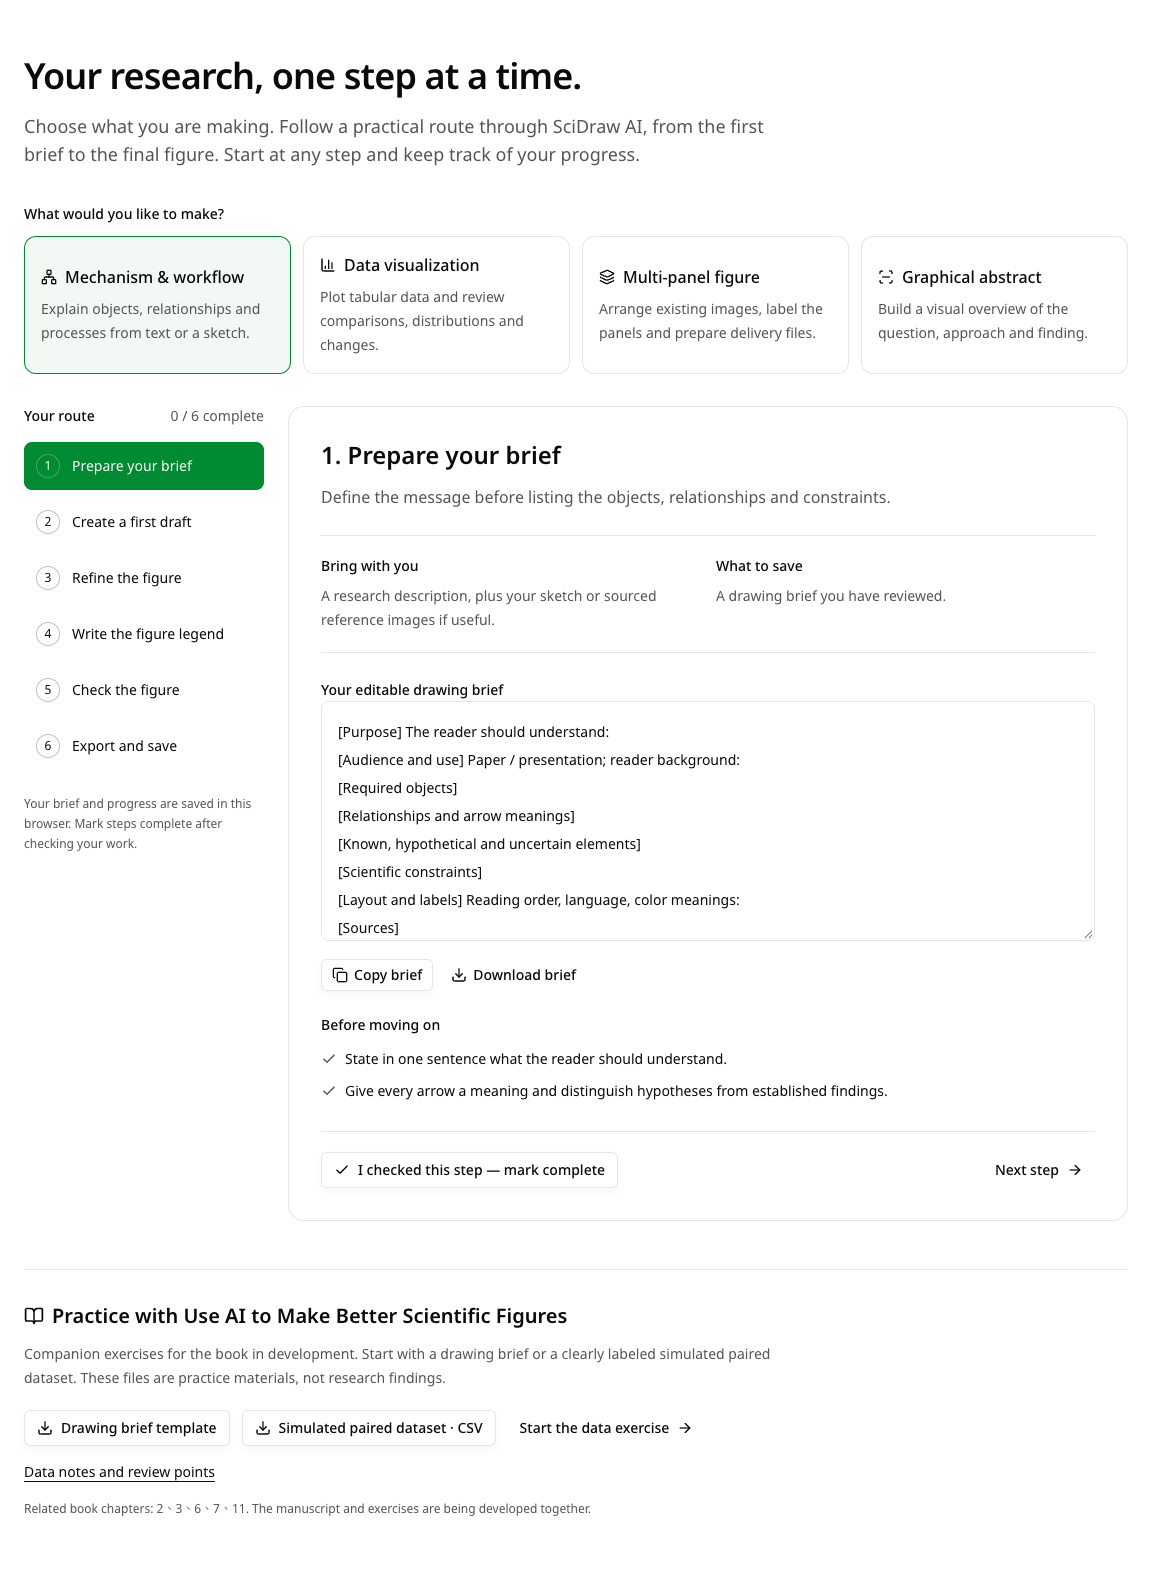
\includegraphics[width=0.92\linewidth,height=0.68\textheight,keepaspectratio]{figures/ch01/ch01-08-guide-ui-en.png}
\caption{The \scidraw{} figure workflow guide (30 October 2026). With ``Mechanism \& workflow diagram'' selected, the page lists a four-step route---Generate a first draft, Refine details, Write the figure legend, Check and export---each with one sentence and a button that opens the tool.}\label{fig:ch01-08}
\end{figure}

A composite figure can chain two routes together: our case followed the ``Data figure'' route into \sdtool{sci-vis} for panel b, then the ``Mechanism \& workflow diagram'' route into \sdtool{workflow-diagram-generator} or \sdtool{ai-drawing} for panel a, before moving to the panel assembly, legend, and checking tools. If you already have a finished plot and only need a legend or resolution check, you can jump directly to that step.

Keep three platform facts in mind when using the guide:
\begin{enumerate}
\item \textbf{The guide stores neither your brief nor your progress:} The page only shows the route and links to the tools; it has no brief editor and does not track which step you have reached. Write the brief in your own document or text file, keep it in the project folder as the record, and paste it into the tool at each step.
\item \textbf{Cross-tool handoff uses download and upload:} The guide's buttons simply open the matching tool; they do not carry your brief or images along. When sending individual panels to the assembly, legend, or checking tools, download clearly named files (such as \texttt{panel-b-nitrate-v2.pdf}) and upload them to the next tool, which also avoids passing outdated drafts.
\item \textbf{The guide does not perform scientific review for you:} It supplies only the order of steps and the tool links; verifying units, quality codes, and evidential boundaries remains the author's job.
\end{enumerate}

\section{Keep a small archive for every figure}

Creating a small folder with a fixed structure on your local drive or code repository for each figure makes it easy to reproduce or revise months later when reviewers ask for changes. The archive structure for this chapter's case is:

\begin{Prompt}
fig2-raccoon-nitrate/
  source/   usgs-05484500-2016.rdb (raw download backup, read-only)
            raccoon-2016-daily.csv, data-dictionary.md (fields, units, flags, DOI, date)
  brief/    figure2-brief-v1.txt (your saved brief), prompts-log.txt (all submitted inputs)
  drafts/   panel-b-draft1.pdf, panel-b-revised.pdf, panel-a-candidates/,
            revision-notes.md (the 8 draft defects and return-path revision log)
  final/    figure2-final.pdf, figure2-final.tiff, legend-zh.txt, legend-en.txt,
            ai-use.md (functions used, dates, inputs, adopted outputs, manual edits), checks.md
  code/     fetch_usgs.py, plot_nitrate.py
\end{Prompt}

You do not need to log every mouse movement, but \textbf{every decision that affects scientific facts or quantitative interpretation must leave a record}: unit conversion formulas and axis transformations, rules for missing values and quality codes, reasons for removing unsupported elements and selecting among generated candidates, and the scope of reference lines. In \texttt{ai-use.md}, record the tool functions used, date, actual inputs, adopted outputs, and manual edits; check your target journal's current AI disclosure policy before submission.

\section{What AI can and cannot do at this stage}

The boundaries among AI, deterministic tools, and the author across the six stages are summarized in Table~\ref{tab:ch01-01}.

\begin{table}[htbp]\centering\footnotesize
\setlength{\tabcolsep}{3pt}
\renewcommand{\arraystretch}{1.15}
\caption{What AI can do, what AI cannot do, and what the author must check across the six stages.}\label{tab:ch01-01}
\begin{tabularx}{\linewidth}{@{}>{\raggedright\arraybackslash}p{20mm}YYY@{}}
\toprule
\textbf{Stage} & \textbf{What AI can do} & \textbf{What AI cannot do} & \textbf{What the author must check} \\
\midrule
Define the task & Draft brief fields from your description; point out missing items (such as units, audience, or size) & Decide the research question the figure should answer; judge whether a claim holds & Whether the task sentence is testable; whether intended use and dimensions are accurate \\
Gather materials & Write download/parsing scripts; tally missing values and quality codes; draft data dictionary & Guarantee the dataset version is right; tell ``as N'' from ``as $\text{NO}_3^-$'' without reading parameter docs & Units, quality codes, download date, and whether provisional data were mixed in \\
Make a draft & Data plots: plot from explicit instructions; schematics: quickly generate layout candidates & Guarantee no interpolation or smoothing unless told; guarantee schematics omit unsupported objects & Check against acceptance criteria line by line; count raw points; look for added objects \\
Check and revise & Execute specific revision commands; regenerate plots or images from a defect list & Judge whether an edit introduced new errors; change one spot without affecting the rest of an image & Re-verify the entire figure after every edit, including parts not meant to change \\
Assemble and explain & Grid layout, panel lettering, size presets; draft figure legends & Know station IDs, download dates, or processing rules invisible in the image; fabricating sample sizes or statistics is forbidden & Whether every number and statement in the legend has a documented source \\
Check and deliver & Technical checks (resolution, color mode, grayscale, color-vision risks) & Scientific peer review; confirm journal AI policies for you & Readability at final print size; whether others can reproduce the figure from the delivery pack \\
\bottomrule
\end{tabularx}
\end{table}

\section{Checklist}

\begin{itemize}
\item I can write the goal of this figure in one sentence, and it constrains the chart type, layout, or labels.
\item I have identified the material category of each panel; data panels use deterministic plotting, and schematic panels depict no unsupported objects.
\item An unaltered copy of the raw data is preserved; units, quality codes, missing values, and download dates are written in the data notes.
\item Every input actually submitted to a tool has been saved.
\item Every revision round is recorded: what changed, why, and which stage the workflow returned to.
\item The final figure has been checked for text and line legibility at its actual print dimensions.
\item Every number, source, and processing note in the figure legend is backed by the archive.
\item I moved on from each step only after checking its output against the brief, not merely because a tool page had been opened.
\item The delivery package includes an AI-use log, and I checked the target journal's current requirements before submission.
\end{itemize}

\section{Exercises}

\begin{enumerate}
\item \textbf{(Task sentences)} Write two alternative task sentences for this chapter's case: one focused on ``how many days high concentrations persist in spring,'' and another focused on ``concentrations during low-flow periods.'' Explain how each would change the chart type, time range, or annotations.
\item \textbf{(Finding defects)} Without looking at the revision table in Section 1.4, list at least five problems across Figure~\ref{fig:ch01-03} and Figure~\ref{fig:ch01-05}, write one verifiable revision instruction for each, and state which of the six stages each problem should return to.
\item \textbf{(Hands-on with \scidraw{})} Download one year of daily mean data from another USGS station with a nitrate sensor (or use a time series from your own research). Write a brief in your own document following the format in Section 1.4, then choose ``Data figure'' in the figure workflow guide (\sdtool{figure-workflow}), follow step 1 into \sdtool{sci-vis}, upload the data, and paste in the plotting requirements from your brief. Check the output against your acceptance criteria item by item, record at least one revision instruction and its effect, and archive the entire process using the folder structure in Section 1.6.
\end{enumerate}

\section*{References}

\begin{itemize}
\item Pellerin BA, Stauffer BA, Young DA, Sullivan DJ, Bricker SB, Walbridge MR, Clyde GA, Shaw DM. Emerging tools for continuous nutrient monitoring networks: sensors advancing science and water resources protection. \textit{JAWRA Journal of the American Water Resources Association}. 2016;52(4):993--1008. \url{https://doi.org/10.1111/1752-1688.12386}
\item Rougier NP, Droettboom M, Bourne PE. Ten simple rules for better figures. \textit{PLoS Computational Biology}. 2014;10(9):e1003833. \url{https://doi.org/10.1371/journal.pcbi.1003833}
\item Schilling K, Zhang Y-K. Baseflow contribution to nitrate-nitrogen export from a large, agricultural watershed, USA. \textit{Journal of Hydrology}. 2004;295(1--4):305--316. \url{https://doi.org/10.1016/j.jhydrol.2004.03.010}
\item U.S. Environmental Protection Agency. National Primary Drinking Water Regulations (nitrate MCL 10 mg/L as N). \url{https://www.epa.gov/ground-water-and-drinking-water/national-primary-drinking-water-regulations}
\item U.S. Geological Survey. USGS water data for the Nation: National Water Information System database, site 05484500. \url{https://doi.org/10.5066/F7P55KJN} (accessed 2026-10-29).
\item Weissgerber TL, Milic NM, Winham SJ, Garovic VD. Beyond bar and line graphs: time for a new data presentation paradigm. \textit{PLOS Biology}. 2015;13(4):e1002128. \url{https://doi.org/10.1371/journal.pbio.1002128}
\end{itemize}

\chapter{Turn research content into a drawing brief}

\begin{BookNote}
R, K, P, and I are abstract teaching symbols. They do not represent real molecules or a published mechanism. The included illustration is an actual Codex image-generation output, reviewed against these fictional requirements.
\end{BookNote}

Researchers can often explain a project to a colleague in a few minutes yet struggle to tell a drawing tool what to show. A conversation allows us to supply missing assumptions and rely on shared background. A drawing instruction must make those assumptions explicit.

“Draw a pathway showing upstream activation, downstream effects, and an inhibitor” sounds like a task. But what is upstream? Which object is activated? Is the downstream effect observed or proposed? Where does the inhibitor act? Without answers, the generator must fill in structure.

A drawing brief turns the author's knowledge into instructions that can be executed and checked.

\section{Give the brief and the prompt different jobs}

The brief records what you intend to communicate and the basis for it. A prompt selects relevant parts of that brief for a particular operation. They may be nearly identical, or differ substantially across stages.

Initial generation needs objects, relationships, and layout. A color revision may need only a new color assignment and the elements that must remain unchanged. A legend requires the image and an explanation of its context. The brief keeps these local operations aligned with the same purpose.

There is no need to force every requirement into one universal prompt. Write the brief first, then select information for the current operation. If a revision changes the scientific content, update the brief as well, so that an old specification does not continue to drive a new image.

\section{Build the brief around seven questions}

The companion template contains ten fields. These seven questions organize the thinking behind them.

\textbf{Who will read it, and where?} A specialist, an interdisciplinary reviewer, and a student may need different figures from the same study. Use also determines viewing size. “For colleagues familiar with the basic method, in the results section of a paper” is more informative than “journal style.”

\textbf{What is the main question?} State the figure's central task in one sentence. If the sentence accumulates several separate aims, consider panels with distinct jobs.

\textbf{Which materials support it?} Identify filenames, worksheets, records, or locations in references. The aim is to support important statements, not to maximize the volume of uploaded material. Avoid mixing incompatible result versions.

\textbf{Which objects and relationships are required?} A list of objects is insufficient without correspondence, direction, grouping, or spatial placement. Two measurements from the same object constitute a relationship, just as an arrow does in a mechanism diagram.

\textbf{What is observation, and what is interpretation?} Keep observations, inferences, and hypotheses distinct. State uncertainty in the brief, express it with labels or an agreed line style, and explain the convention in the legend. A tool should not decide an unsupported relationship.

\textbf{How should it be presented?} Now choose chart type, reading direction, panels, color roles, and label language. Give constraints that help explain the content. Adjectives alone cannot specify a layout.

\textbf{How will completion be recognized?} Write criteria such as correct object counts, one-to-one correspondence with the relationship table, preservation of every value, and readable text at final size. Connect review criteria to the source materials.

Mark unresolved information as “to be confirmed.” It becomes a task for the author rather than an invitation for a polished draft to settle the matter.

\section{Replace a noun list with a relationship table}

Consider a deliberately fictional model with four symbols: R, K, P, and I. For this exercise, R activates K; K has a hypothetical influence on P; and I inhibits K. These are teaching assumptions, not biological claims.

“R, K, P, I; mechanism diagram; blue-green; simple” does not determine the connections. A relationship table does.

\begin{center}\small
\begin{tabularx}{\linewidth}{l l Y Y}
\toprule
\textbf{From} & \textbf{To} & \textbf{Meaning in this model} & \textbf{Visual convention} \\
\midrule
R & K & Given activation & Solid arrow toward K \\
K & P & Hypothetical influence & Dashed arrow toward P \\
I & K & Given inhibition & Line ending in a T-bar at K \\
\bottomrule
\end{tabularx}
\end{center}

\begin{figure}[htbp]\centering
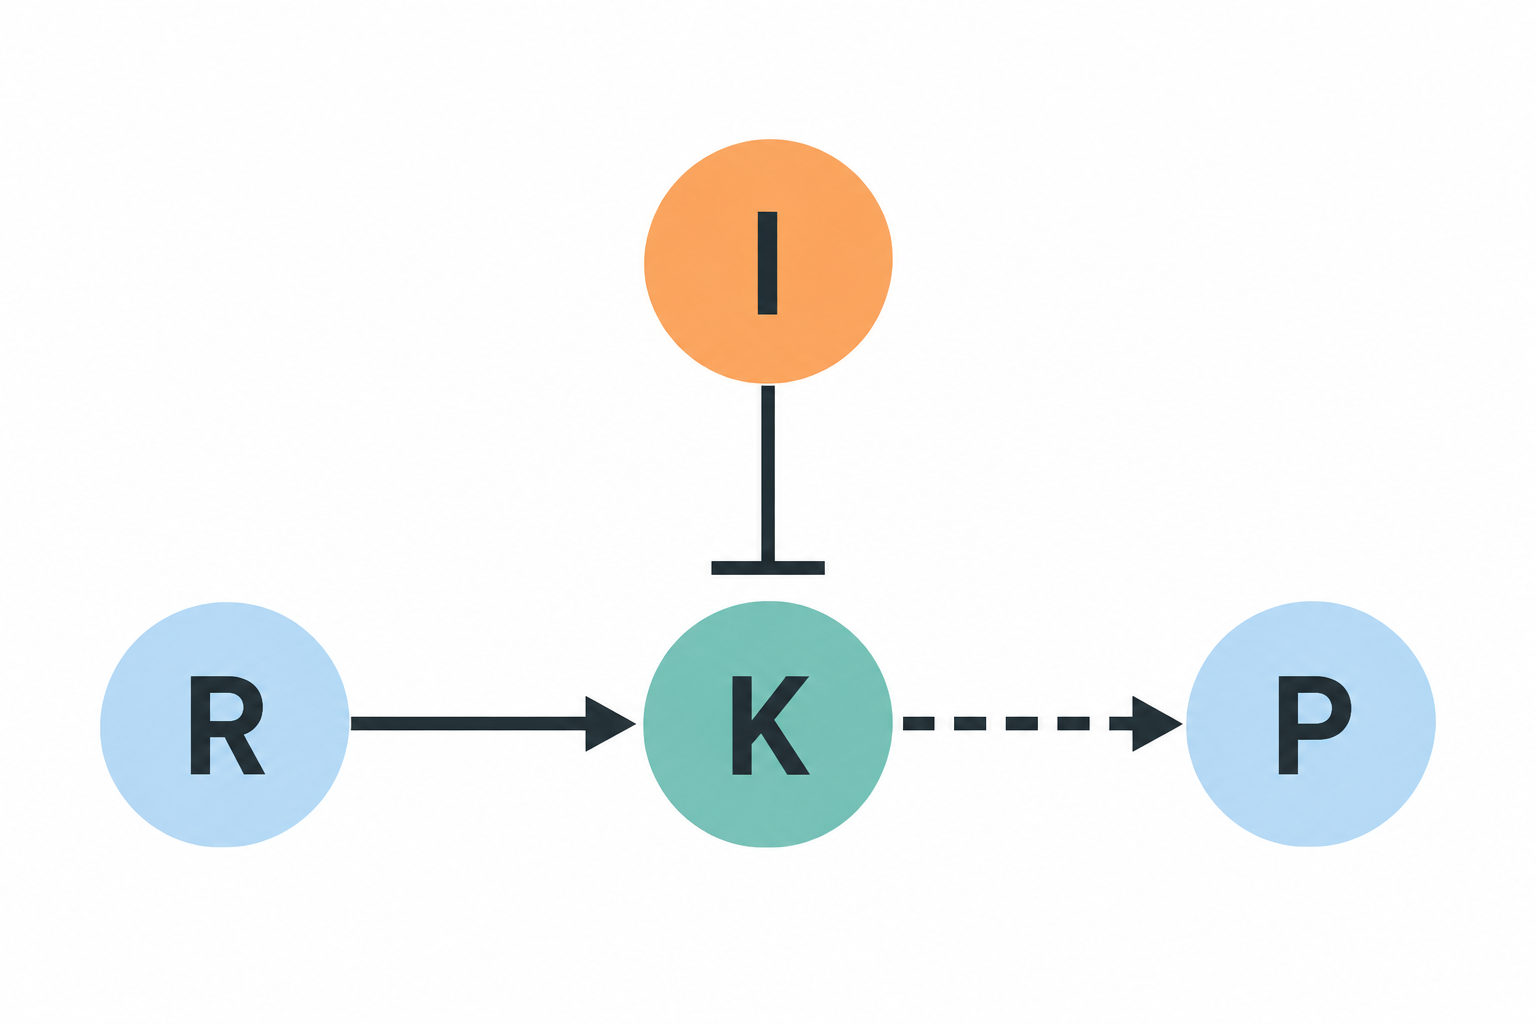
\includegraphics[width=\linewidth]{figures/mechanism-codex.png}
\caption{An actual candidate from Codex's built-in image generation. A solid arrow, dashed arrow, and T-bar express the three stipulated relationships. All four symbols and relationships are fictional. This output was generated in Codex, not in SciDraw AI.}
\label{fig:mechanism}
\end{figure}

Line styles and arrowheads have no universal meaning outside context. Their meaning depends on disciplinary convention, the definitions in the figure, and its legend. The conventions here distinguish three relationships. A real project should use forms its audience understands and add explicit labels where ambiguity remains.

Review the result row by row: locate R and K and inspect the direction; check that the K-to-P connection remains dashed; then confirm that I's inhibitory endpoint is K. “Does this look right?” becomes a set of locatable questions.

\section{Write an executable instruction for the mechanism}

Select the mechanism-and-workflow route in the SciDraw AI guide, replace its default brief, and download a copy.

\begin{Prompt}
[Audience and use] Scientific-figure teaching; no biology background required.
[Purpose] Distinguish given, hypothetical, and inhibitory relationships.
[Source] Only the fictional model specified here.
[Objects] R, K, P, I; each appears once.
[Relationships]
R activates K: a solid arrow from R to K.
K may influence P: a dashed arrow from K to P.
I inhibits K: a line ending with a perpendicular T-bar next to K.
[Layout] R, K, P from left to right; I above K.
[Visual language] White background; simple two-dimensional shapes; identify every object by its letter.
[Constraints] Add no objects, relationships, molecular forms, or experimental results.
[Legend] Explain the three line conventions and identify the fictional teaching model.
[Review] Four objects and three relationships; check direction, endpoints, and labels.
\end{Prompt}

This instruction provides concrete quality criteria: identifiable objects, accurate relationships, and a hypothesis that remains distinguishable from a given relationship. Color can be refined later; the relationships must hold first.

In the mechanism tool, place the instruction in the generation field. Review a candidate against the relationship table before requesting further changes. If an extra object appears, identify it and restate the requirement for exactly four objects, rather than asking only for a simpler design.

For this edition, Codex's built-in image generator produced Figure~\ref{fig:mechanism}. The complete executed prompt and review are included in the repository. The four labels and three relationship types match the brief. Soft tonal variation remains inside the nodes, so this is a checked teaching candidate, not proof that every style constraint was followed exactly. It is not a SciDraw AI output.

The executed generation prompt uses labels alone, with the explanatory words moved to the caption. This is an intentional layout choice recorded in the provenance. Outputs can vary between runs; an instruction does not guarantee that all requirements will be met automatically.

\section{For a data plot, specify constraints by column}

A data brief must connect study design to table structure. Three columns in the first exercise already illustrate several possible ambiguities.

\texttt{sample\_id} identifies an object. \texttt{before} and \texttt{after} contain its two measurements. Eight rows represent eight fictional objects and sixteen observations. State object and measurement counts separately. In real research, also explain experimental units, repeated measurements, and technical replicates.

\begin{Prompt}
Read the uploaded paired-example.csv.
sample_id is the pairing key. before and after are two measurements in a.u.
Create a paired point-and-line plot, with before then after on the x-axis.
Connect the two observations belonging to each object.
Keep all eight objects and the sixteen original values.
Do not treat the columns as independent samples or connect different objects.
Title: "Simulated teaching data: individual changes".
Show the measurements without significance tests or error bars.
Do not remove SIM04 or change its decrease into an increase.
\end{Prompt}

The final line is a check against the file: SIM04 really does decrease from 18 to 17 in this exercise. It does not prescribe a desired finding for real research. Define checks from your actual data, rather than forcing the figure to match an expected conclusion.

“No error bars” is also specific to this exercise. When a different plot needs them, define whether they represent standard deviation, standard error, a confidence interval, or another quantity, and identify how it is calculated. “Add standard error bars” cannot be used as a vague synonym for any uncertainty interval.

\section{When using a PDF helper, establish what was read}

A paper's information is distributed across its abstract, body, figures, methods, and supplementary materials. How text is extracted affects the content available to a visual-prompt helper.

The SciDraw AI PDF helper examined for this edition reads up to the first five pages and uses a limited extract from the abstract or beginning of the document. It can assist with a research overview, but this does not establish that the entire paper, every figure, and the supplements have been interpreted.

Before using it, prepare author-confirmed points: the research question, main method, result to show, and relevant conditions. Compare the helper's prompt with that list, restore omitted information, and only then proceed to drawing. A key result appearing later in a paper may be absent from an input limited to its opening pages.

Record the input scope in the brief. For example: “Author-prepared abstract and result notes; PDF assistance used for drafting; key statements checked against the original.” This is more accurate than “automatically generated from the full paper” and makes future reconstruction easier.

\section{Turn vague feedback into reviewable requests}

Repeated generation can become a search for a more appealing image without a clear purpose. Give each operation a defined job.

\begin{center}\small
\begin{tabularx}{\linewidth}{p{0.25\linewidth}Y}
\toprule
\textbf{Vague feedback} & \textbf{A more concrete request} \\
\midrule
More professional & Align R, K, and P horizontally; use one label size; retain all objects and relationships. \\
Emphasize the result & Make the two measurements directly comparable while retaining individual lines and all observations. \\
Simplify it & Remove decorative backgrounds and repeated explanation; retain four objects, three relationships, and the legend. \\
Journal style & Use a white background and less decoration; apply the agreed text hierarchy and color roles. \\
Complete the legend & Draft what can be identified from the image; the author supplies sample sizes, conditions, and statistical methods. \\
\bottomrule
\end{tabularx}
\end{center}

These requests do not guarantee error-free execution. They make execution assessable. Image edits can affect the whole image, so even a request to change one label should be followed by another check of objects and relationships.

\section{Read the brief as if the research were unfamiliar}

Temporarily set aside the background in your head and look for missing information in the text.

“The treatment group is higher” lacks a variable, condition, and evidential basis. “Split into two groups after this step” lacks a grouping rule. “Improves performance” lacks a metric, unit, and comparison. Supply the missing information or mark the claim as unresolved.

A small mapping table can help: statement, source location, visual representation, and question still to resolve. In real projects, identify a column, file version, or record page. In this exercise, identify a teaching assumption. This prevents poorly sourced claims from slipping into an image.

\section{Exercise and acceptance criteria}

Complete two briefs: one for your research and one for either the fictional mechanism or paired-data example. Retain the original description and write a short revision note explaining which relationships, sources, and acceptance criteria you added.

Check whether objects can be counted, relationships can be examined one by one, data constraints map to columns, unknowns remain explicit, and the output has a concrete use.

You now have an input that can move into figure creation. Chapter 3 will explore different compositions from the same brief and compare the work they ask the reader to do.

\chapter{Working Out Layout and Sketches with AI}
\usetikzlibrary{decorations.pathreplacing}

Lin Yue, a doctoral student in molecular biology, is preparing her dissertation proposal and drafting the introduction to a review on genome editing. She needs Figure 1: a full-width overview schematic showing life-science peers and reviewers how \emph{Streptococcus pyogenes} Cas9 (SpCas9), guided by a single guide RNA (sgRNA), recognizes a protospacer-adjacent motif (PAM) and cleaves double-stranded DNA, and how non-homologous end joining (NHEJ) and homology-directed repair (HDR) yield distinct editing outcomes.

She opens an image generator and enters a single prompt: ``Draw a professional, visually striking overview figure of the CRISPR--Cas9 genome editing mechanism suitable for a top journal.'' Seconds later, the tool returns a glossy landscape illustration: inside a three-dimensional dark-blue cell nucleus, glowing cyan scissors slice through a twisted DNA helix, while the four corners hold a ribbon-like RNA strand, a glowing ``PAM'' badge, and two short DNA fragments—one cracked and one patched with color.

Impressed by the surface polish, Lin Yue drops the image into her slides. Her advisor looks at the screen for five seconds and asks: ``Where am I supposed to start reading this figure?''

Lin Yue hesitates. Her advisor points out the visual traps: a reader's eye goes straight to the largest, brightest element at the center—the glowing scissors—even though cleavage is the third step. After the scissors, should the eye move to the top-left corner for the RNA, or to the bottom-right corner for the repaired DNA? Worse, the two repaired DNA fragments sit in the bottom-left and bottom-right corners with no connecting arrows and no shared baseline. How can a reader tell that they represent parallel repair choices branching from one break, rather than sequential steps?

This first draft fails not from poor rendering, but because the author clicked ``Generate'' before deciding the reader's entry point and eye path. Without a spatial skeleton, an image model defaults to decorative symmetry—placing a dramatic object at the center and scattering the remaining nouns into the corners. This chapter moves layout exploration and sketching ahead of rendering, addressing five questions: how to control reading order via ``entry--path--endpoint,'' how to decide what belongs in one panel, how to draw three distinct layout sketches from a single brief, how to generate and evaluate candidates in \scidraw{}, and how to revise with one verifiable goal per pass.

\section{Reading Order Comes Before Rendering}

When readers encounter an overview figure, they do not scan it word by word like text. In the first few seconds, vision follows instinct: the eye lands on the heaviest visual anchor and follows geometric cues across the canvas (Wong, 2011c; Rougier et al., 2014). If a figure cannot show ``where to start, where to go, and where to stop'' within five seconds, even finely rendered molecules will impede comprehension.

Before sketching or prompting, plan the viewer's trajectory by answering three questions:

\begin{itemize}
\item \textbf{First, where is the entry point?} The first fixation lands on the region of greatest visual weight—usually the largest shape, strongest luminance or color contrast, most isolated element, or conventional starting corner (top-left or far-left in horizontal layouts). Without a clear anchor, or when three or four equally prominent blobs compete for attention, the reader hesitates immediately.
\item \textbf{Second, how does the path move?} Once inside the frame, the eye needs geometric guides. Explicit guides include unidirectional arrows and step numbers (1, 2, 3, and so on); implicit guides include shared horizontal or vertical alignment baselines, continuous white-space channels, and natural left-to-right or top-to-bottom progression.
\item \textbf{Third, where does the path end?} The final resting point should hold the core scientific takeaway. Inflating upstream background components while cramping the final comparison or repair outcomes into a corner inverts the visual hierarchy, reducing the main message to a footnote.
\end{itemize}

\begin{figure}[htbp]\centering
\resizebox{\linewidth}{!}{% FIG ch03-01 reading order (English)
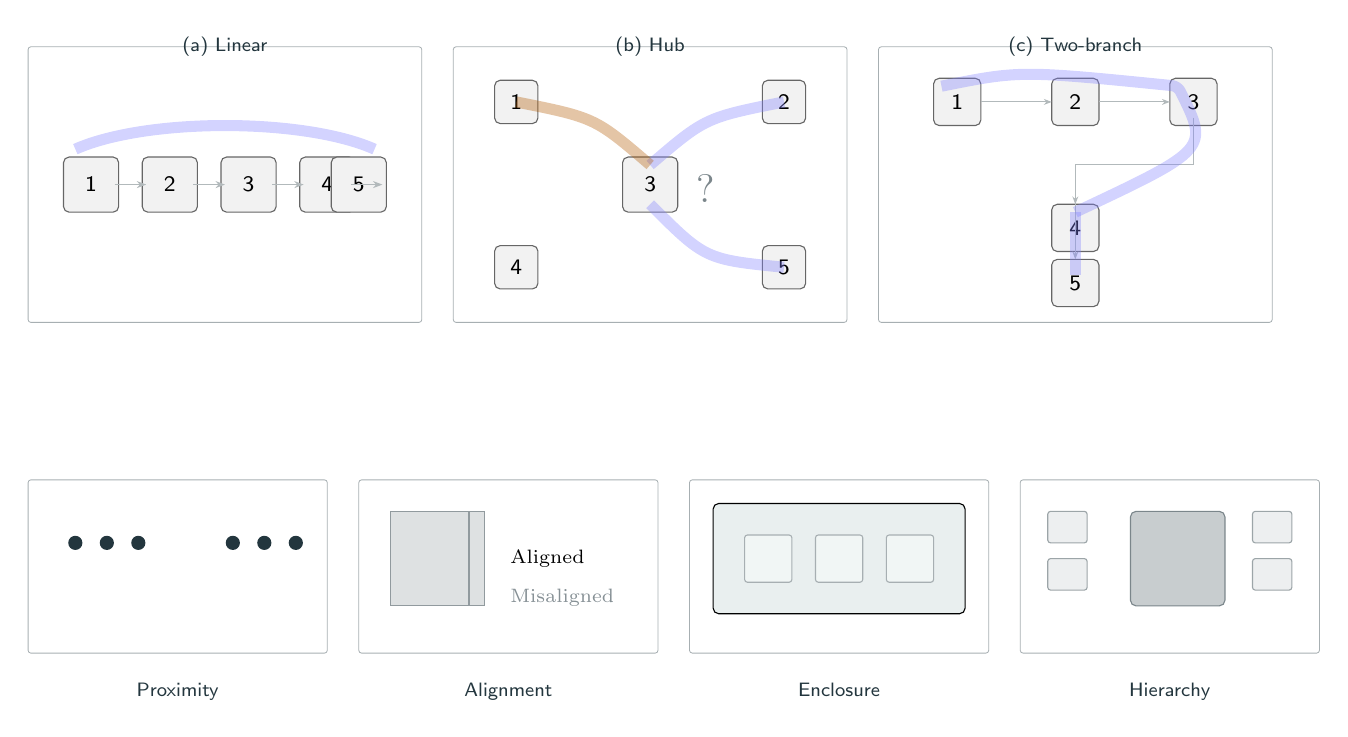
\begin{tikzpicture}[
  x=1mm, y=1mm,
  font=\sffamily\footnotesize,
  panel/.style={draw=BookInk!40, line width=0.3pt, rounded corners=1pt},
  block/.style={
    rounded corners=2pt, draw=black!60, fill=black!5,
    minimum size=7mm, inner sep=0pt, font=\sffamily\footnotesize,
  },
  eye/.style={line width=4pt, draw=blue!50, opacity=0.35, rounded corners=2pt},
  paneltitle/.style={font=\sffamily\scriptsize, text=BookInk, align=center},
]
  \def\pw{50}\def\ph{35}
  \begin{scope}[shift={(0,42)}]
    \draw[panel] (0,0) rectangle (\pw,\ph);
    \node[paneltitle, anchor=north] at (0.5*\pw,\ph+2.5) {(a) Linear};
  \end{scope}
  \begin{scope}[shift={(54,42)}]
    \draw[panel] (0,0) rectangle (\pw,\ph);
    \node[paneltitle, anchor=north] at (0.5*\pw,\ph+2.5) {(b) Hub};
  \end{scope}
  \begin{scope}[shift={(108,42)}]
    \draw[panel] (0,0) rectangle (\pw,\ph);
    \node[paneltitle, anchor=north] at (0.5*\pw,\ph+2.5) {(c) Two-branch};
  \end{scope}
  \begin{scope}[shift={(0,42)}]
    \foreach \i/\x in {1/8,2/18,3/28,4/38,5/42} {
      \node[block] at (\x,17.5) {\i};
    }
    \draw[eye] (6,22) .. controls (15,26) and (35,26) .. (44,22);
    \foreach \i/\xa/\xb in {1/11/15,2/21/25,3/31/35,4/41/45} {
      \draw[-{Stealth[length=1.2mm]}, draw=BookInk!35, thin] (\xa,17.5) -- (\xb,17.5);
    }
  \end{scope}
  \begin{scope}[shift={(54,42)}]
    \node[block] at (25,17.5) {3};
    \node[block, minimum size=5.5mm] at (8,28) {1};
    \node[block, minimum size=5.5mm] at (42,28) {2};
    \node[block, minimum size=5.5mm] at (8,7) {4};
    \node[block, minimum size=5.5mm] at (42,7) {5};
    \draw[eye, blue!50] (25,20) .. controls (32,26) .. (42,28);
    \draw[eye, orange!70!black, opacity=0.35] (25,20) .. controls (18,26) .. (8,28);
    \draw[eye, blue!50] (25,15) .. controls (32,8) .. (42,7);
    \node[font=\Large, text=BookInk!60] at (32,17) {?};
  \end{scope}
  \begin{scope}[shift={(108,42)}]
    \foreach \i/\x in {1/10,2/25,3/40} {
      \node[block, minimum size=6mm] at (\x,28) {\i};
    }
    \node[block, minimum size=6mm] at (25,12) {4};
    \node[block, minimum size=6mm] at (25,5) {5};
    \draw[-{Stealth[length=1mm]}, draw=BookInk!35, thin] (13,28) -- (22,28);
    \draw[-{Stealth[length=1mm]}, draw=BookInk!35, thin] (28,28) -- (37,28);
    \draw[-{Stealth[length=1mm]}, draw=BookInk!35, thin] (40,26) -- (40,20) -- (25,20) -- (25,15);
    \draw[-{Stealth[length=1mm]}, draw=BookInk!35, thin] (25,20) -- (25,8);
    \draw[eye] (8,30) .. controls (18,32) .. (38,30) .. controls (42,22) .. (25,14);
    \draw[eye] (25,14) -- (25,6);
  \end{scope}
  \def\bw{38}\def\bh{22}
  \foreach \i/\x/\title in {
    1/0/Proximity, 2/42/Alignment, 3/84/Enclosure, 4/126/Hierarchy} {
    \begin{scope}[shift={(\x,0)}]
      \draw[panel] (0,0) rectangle (\bw,\bh);
      \node[paneltitle, anchor=north] at (0.5*\bw,-2.5) {\title};
    \end{scope}
  }
  \begin{scope}[shift={(0,0)}]
    \foreach \x in {6,10,14} {\fill[BookInk] (\x,14) circle (0.9mm);}
    \foreach \x in {26,30,34} {\fill[BookInk] (\x,14) circle (0.9mm);}
  \end{scope}
  \begin{scope}[shift={(42,0)}]
    \draw[fill=BookInk!15, draw=BookInk!50] (4,6) rectangle (16,18);
    \draw[fill=BookInk!15, draw=BookInk!50] (4,6) rectangle (14,18);
    \node[font=\scriptsize, anchor=west] at (18,12) {Aligned};
    \node[font=\scriptsize, anchor=west, text=BookInk!55] at (18,7) {Misaligned};
  \end{scope}
  \begin{scope}[shift={(84,0)}]
    \draw[fill=BookRule!40, rounded corners=2pt] (3,5) rectangle (35,19);
    \foreach \x in {10,19,28} {
      \draw[fill=BookPale, draw=BookInk!40, rounded corners=1pt] (\x-3,9) rectangle (\x+3,15);
    }
  \end{scope}
  \begin{scope}[shift={(126,0)}]
    \draw[fill=BookInk!25, draw=BookInk!60, rounded corners=2pt] (14,6) rectangle (26,18);
    \foreach \x/\y in {6/16,6/10,32/16,32/10} {
      \draw[fill=BookInk!8, draw=BookInk!45, rounded corners=1pt] (\x-2.5,\y-2) rectangle (\x+2.5,\y+2);
    }
  \end{scope}
\end{tikzpicture}
}
\caption{Layout decides reading order. Top: the same five elements arranged in three structures; translucent curves show the most likely eye path. The hub layout has no single entry point, so readers may take different routes. Bottom: four basic ways to control hierarchy and grouping.}\label{fig:ch03-01}
\end{figure}

The upper row of Figure~\ref{fig:ch03-01} shows how arranging the same five sequential nodes (1 to 5) into three structures alters the eye path. In the \textbf{linear layout} (Figure~\ref{fig:ch03-01}a), five rounded blocks sit in a single row linked by gray arrows; the translucent blue curve traces an unambiguous left-to-right trajectory from node 1 to node 5, ideal for unbranched sequences.

Now consider the \textbf{hub layout} (Figure~\ref{fig:ch03-01}b), where node 3 sits enlarged at the center and nodes 1, 2, 4, and 5 occupy the four corners. While common in mind maps, this structure disrupts sequential processes. As the conflicting blue and orange curves show, readers take different routes: some start at the large central node 3 and jump toward 2 or 5; others start by habit at top-left node 1, pass through 3, and stall—marked by the question mark—unsure whether to go to the upper right or lower left. Without a unique entry point, readers must guess the sequence.

Figure~\ref{fig:ch03-01}c shows a \textbf{two-branch layout} suited for ``shared upstream pathway, two alternative outcomes.'' Nodes 1, 2, and 3 form a compact top row from left to right; from node 3, a downward arrow splits into two parallel branches feeding vertically stacked nodes 4 and 5. The eye scans the upstream sequence horizontally, follows the fork downward, and immediately reads 4 and 5 as parallel outcomes from node 3.

With the skeleton in place, four visual mechanisms govern internal order (Figure~\ref{fig:ch03-01}, bottom row), drawing on Gestalt perception (Wong, 2010a, 2010b) and visual hierarchy (Wong, 2011d):

\begin{enumerate}
\item \textbf{Proximity:} Nearby elements are grouped automatically. In the first bottom panel of Figure~\ref{fig:ch03-01}, six dots divide into two triplets solely through tight internal spacing and a wide central gap. In scientific figures, open background (negative space) is not wasted paper; it is the divider separating stages or complexes (Wong, 2011b). When a generator packs objects evenly across the canvas, losing proximity contrast makes the image look chaotic.
\item \textbf{Alignment:} Elements sharing a horizontal baseline or vertical left edge are read as comparable peers (Figure~\ref{fig:ch03-01}, second bottom panel). When comparing two DNA repair outcomes, aligning the left and right endpoints of both duplexes lets readers spot the central change instantly; staggered or unequal strands make readers wonder whether the offset implies biological truncation.
\item \textbf{Enclosure:} Framing elements inside a tinted box or thin rectangle is the strongest grouping cue (Figure~\ref{fig:ch03-01}, third bottom panel). When a repair pathway includes a cleaved substrate, an exogenous donor template, and a repaired duplex, enclosing the lane keeps the floating donor from being misassigned to the adjacent pathway.
\item \textbf{Hierarchy:} A figure should have only one center of primary visual weight (Figure~\ref{fig:ch03-01}, fourth bottom panel). Adding more bright colors only makes every object compete. Instead, combine \textbf{size, luminance contrast, and position}: give the main comparison the largest area and whitespace, reserve high-contrast accents for active changes (such as the PAM, indel scar, or inserted sequence), and mute invariant scaffolding in neutral gray.
\end{enumerate}

These four mechanisms reduce to one rule: \textbf{grouping is a scientific claim.} Objects placed close together, aligned on a baseline, enclosed in a frame, or given the same color will be read as scientifically related. Likewise, causal sequences should follow left-to-right or top-to-bottom reading direction, and parallel branches must share symmetrical geometry so options are not misread as sequential steps.

Before refining a draft, run three quick self-tests: (1) the \textbf{five-second test}—show the draft to a colleague unfamiliar with the brief for five seconds, hide it, and ask what they saw first and what the figure compares; (2) \textbf{finger tracing}—ask the colleague to trace their eye path with a finger, noting any pause or backtrack as a broken layout cue; and (3) the \textbf{half-scale grayscale check}—shrink the figure to 50\% of its print width (e.g., 87 mm for a 174 mm figure) in grayscale to confirm a single visual center and clear white-space channels.

\section{What Belongs in One Panel}

Once reading order is set, we must decide how much to include. The second common flaw in overview figures is overcrowding: trying to show plasmid or ribonucleoprotein (RNP) delivery across the cell membrane, nuclear pore entry, chromosome and nucleosome unwinding, a 3D Cas9 crystal structure with HNH and RuvC catalytic residues, repair factors (Ku70/80, DNA-PKcs, Ligase IV), microhomology-mediated end joining (MMEJ), off-target cleavage, and base editing—all inside one 174 mm panel. Cramming thirty multi-scale objects together makes both the overall pathway and the molecular geometry illegible.

The rule is simple: \textbf{one panel answers one core question; only elements that the reader must see simultaneously to follow the causal chain or compare outcomes belong in the same panel.}

Using the one-sentence template from Chapter 1, Lin Yue states the testable task for her Figure 1:

\begin{BookNote}
After viewing this figure, the reader should be able to understand \textbf{how a single guide RNA (sgRNA) directs Cas9 to recognize a target sequence adjacent to a PAM and generate a double-strand break, after which non-homologous end joining (NHEJ) and homology-directed repair (HDR) produce either imprecise small insertions/deletions or precise template-directed edits}, and be able to locate \textbf{the chronological order of events, the relative positions of the PAM and cleavage site, and the sequence-level difference between the two repair outcomes}.
\end{BookNote}

This overview reports no new experimental data; every relationship rests on established textbook and review consensus: Jinek et al.\ (2012) showed that SpCas9 is a dual-RNA- or sgRNA-guided endonuclease that requires a PAM on the non-target strand and uses HNH and RuvC-like domains to cleave the target and non-target strands, respectively; Ran et al.\ (2013) defined practical SpCas9 design rules, placing double-strand cleavage about 3 base pairs (bp) upstream of the $5'$-NGG-$3'$ PAM; Doudna and Charpentier (2014) and Hsu et al.\ (2014) summarized how Cas9 breaks route into NHEJ or HDR outcomes; and Chang et al.\ (2017) detailed the fidelity and mechanisms of NHEJ versus alternative end-joining pathways.

Before sketching, the author compiles these established facts into nine verifiable relationships (Table~\ref{tab:ch03-01-rel}, C1--C9).

\begin{table}[htbp]\centering\footnotesize
\setlength{\tabcolsep}{3pt}
\renewcommand{\arraystretch}{1.15}
\caption{Relationship table (C1--C9) for the CRISPR--Cas9 genome editing overview figure. All relationships represent established consensus; visual simplifications must be declared in the legend.}\label{tab:ch03-01-rel}
\begin{tabularx}{\linewidth}{@{}l>{\raggedright\arraybackslash}p{24mm}>{\raggedright\arraybackslash}p{24mm}>{\raggedright\arraybackslash}p{20mm}Y@{}}
\toprule
\textbf{\#} & \textbf{Source / Input} & \textbf{Target / Outcome} & \textbf{Relationship \& Status} & \textbf{Visual Simplification in This Figure} \\
\midrule
C1 & sgRNA (fused crRNA:tracrRNA strand) & Cas9 protein & Binds to form Cas9--sgRNA complex (Established) & Omit sgRNA secondary-structure details; draw as an orange strand with spacer and hairpin loop \\
C2 & Cas9--sgRNA complex & Genomic DNA PAM ($5'$-NGG-$3'$ for SpCas9) & Recognizes PAM (Established) & Omit 3D diffusion and 1D sliding search along DNA \\
C3 & sgRNA spacer ($\sim$20 nt) & Target DNA strand (complementary to spacer) & Base-pairs to form R-loop; non-target strand displaced (Established) & Omit stepwise zipping kinetics of R-loop formation \\
C4 & Spatial position of PAM & Non-target strand, immediately $3'$ of protospacer & Strand polarity and adjacency (Established) & Show as a yellow highlight in main panel; place exact $5'\rightarrow 3'$ polarity in the inset \\
C5 & Cas9 (HNH and RuvC-like domains) & Both strands cut $\sim$3 bp upstream of PAM & Generates double-strand break, mostly blunt (Established) & Do not separate domains in main panel; distinguish HNH and RuvC in the inset \\
C6 & Double-strand break & NHEJ (non-homologous end joining) & Template-free repair route (Established) & Omit Ku70/80, DNA-PKcs, Ligase IV; omit alternative end joining (MMEJ) \\
C7 & NHEJ repair process & Small insertions or deletions (indels) may arise at break site & Outcome; can cause frameshift in coding exons (Established) & Use ``may''; NHEJ can also rejoin ends accurately, leading to recleavage cycles omitted here \\
C8 & Double-strand break + exogenous donor (with homology arms) & HDR (homology-directed repair) & Template-dependent repair route (Established) & Omit end resection and strand invasion intermediates \\
C9 & HDR repair process & Precise change copied from donor (insertion or replacement) & Outcome; lower frequency than NHEJ in most cells (Established) & Give no efficiency numbers; note lower frequency and S/G2 preference in legend only \\
\bottomrule
\end{tabularx}
\end{table}

Two nuances in Table~\ref{tab:ch03-01-rel} merit care. First, C7 states that indels \emph{may} arise at the break site rather than calling NHEJ invariably error-prone. As Chang et al.\ (2017) note, canonical NHEJ ligates compatible ends with high fidelity; in genome editing, indels accumulate because accurate rejoining restores the intact target and PAM, allowing persistent Cas9--sgRNA to recleave until an indel mutates the site. Although the diagram omits this recleavage loop for simplicity, the text and legend must retain ``may.'' Second, in C9, because HDR efficiency depends on cell type, cell-cycle phase (mainly S/G2), and donor design, the figure omits detached percentage numbers.

Cross-checking the task statement against Table~\ref{tab:ch03-01-rel} divides the material into three streams:

\begin{itemize}
\item \textbf{Stream 1: Keep in the main overview panel.} The main panel shows ``who acts, where, in what order, and with what two outcomes,'' retaining eight core objects: bilobed Cas9 silhouette, orange sgRNA, ladder-like double-stranded DNA, yellow PAM block, double-strand break gap, short double-stranded donor template (dark-gray homology arms with a teal central segment), NHEJ outcome DNA (with a reddish-purple indel mark), and HDR outcome DNA (with a teal inserted segment).
\item \textbf{Stream 2: Move to a detail inset.} Locating ``the relative positions of the PAM and cleavage site'' requires exact molecular geometry: antiparallel $5'\rightarrow 3'$ strands, the $5'$-NGG-$3'$ PAM on the non-target strand immediately $3'$ of the protospacer, the $\sim$20-nt sgRNA spacer paired with the target strand, cleavage $\sim$3 bp upstream of the PAM, and HNH cutting the target strand while RuvC cuts the non-target strand. Putting this in an inset keeps the main canvas clean while making base-level geometry explicit.
\item \textbf{Stream 3: Omit and declare in the legend.} Cells, nuclei, chromosomes, delivery vehicles (plasmids, RNPs, viruses), 3D Cas9 structure, repair enzymes, alternative end joining, off-target cuts, base or prime editing, and efficiency numbers are omitted and listed at the end of the legend.
\end{itemize}

\begin{figure}[htbp]\centering
% FIG ch03-07 PAM inset (English)
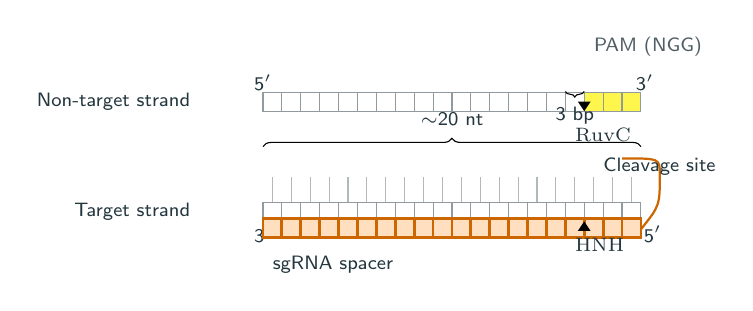
\begin{tikzpicture}[
  x=1mm, y=1mm,
  font=\sffamily\scriptsize,
  text=BookInk,
]
  \node[anchor=east] at (-2, 21.2) {Non-target strand};
  \node[anchor=east] at (-2, 7.2) {Target strand};
  \node at (6, 23.6) {5$'$};
  \node at (54.5, 23.6) {3$'$};
  \node at (55.5, 4.4) {5$'$};
  \node at (6, 4.4) {3$'$};

  \foreach \i in {0,...,19} {
    \pgfmathsetmacro{\x}{6+\i*2.4}
    \draw[draw=BookInk!50, fill=white] (\x,20) rectangle (\x+2.4,22.4);
  }
  \foreach \i in {0,1,2} {
    \pgfmathsetmacro{\x}{6+(17+\i)*2.4}
    \draw[draw=BookInk!50, fill=yellow!70] (\x,20) rectangle (\x+2.4,22.4);
  }
  \node[anchor=west, text=BookInk!80] at (6+17*2.4, 28.2) {PAM (NGG)};

  \foreach \i in {0,...,19} {
    \pgfmathsetmacro{\x}{6+\i*2.4}
    \draw[draw=BookInk!50, fill=white] (\x,6) rectangle (\x+2.4,8.4);
  }
  \foreach \i in {0,...,19} {
    \pgfmathsetmacro{\x}{6+\i*2.4}
    \draw[BookInk!35, thin] (\x+1.2,8.4) -- (\x+1.2,11.6);
    \draw[draw=orange!80!black, fill=orange!25, line width=1pt]
      (\x,4) rectangle (\x+2.4,6.4);
  }
  \draw[orange!80!black, line width=0.8pt]
    (6+19*2.4+2.4, 5) .. controls (6+21*2.4, 8) .. (6+21*2.4, 12)
    .. controls (6+21*2.4, 14) .. (6+19*2.4, 14);

  \node[anchor=west] at (6, 0.5) {sgRNA spacer};
  \pgfmathsetmacro{\cx}{6+16.5*2.4+1.2}
  \fill[black] (\cx,20) -- (\cx-0.8,21.2) -- (\cx+0.8,21.2) -- cycle;
  \fill[black] (\cx,6) -- (\cx-0.8,4.8) -- (\cx+0.8,4.8) -- cycle;
  \node[anchor=west] at (6+17.5*2.4, 13) {Cleavage site};
  \node[anchor=west, font=\scriptsize] at (6+16*2.4, 17) {RuvC};
  \node[anchor=west, font=\scriptsize] at (6+16*2.4, 3) {HNH};

  \draw[decorate, decoration={brace, amplitude=3pt}] (6, 15.5) -- (6+20*2.4, 15.5)
    node[midway, above=4pt] {$\sim$20 nt};
  \draw[decorate, decoration={brace, amplitude=2pt, mirror}] (6+16*2.4, 22.5) -- (6+17*2.4, 22.5)
    node[midway, below=2pt] {3 bp};
\end{tikzpicture}

\caption{Positions of the PAM and the cleavage site (SpCas9). The sgRNA spacer pairs with the target strand; the PAM ($5'$-NGG-$3'$) lies on the non-target strand immediately $3'$ of the protospacer. Both strands are cut about 3 bp upstream of the PAM, the target strand by the HNH domain and the non-target strand by the RuvC-like domain. Schematic; lengths not to scale.}\label{fig:ch03-07}
\end{figure}

Extracting the inset also reflects a critical tool-selection rule: \textbf{exact geometric relationships (strand polarity, which strand carries the PAM, and cut-site distance) should never be left to an image generation model; they must be drawn with deterministic tools.} Image models do not understand antiparallel nucleic acid rules and routinely place $5'$ and $3'$ on the same end, put the PAM on the wrong strand, or cut far from the PAM.

Figure~\ref{fig:ch03-07} shows the deterministic TikZ inset: the upper non-target strand runs $5'\rightarrow 3'$ left to right, with three yellow boxes at the $3'$ end of the 20-box protospacer labeled ``PAM (NGG)''; the lower target strand runs $3'\rightarrow 5'$ left to right; beneath it, the 20-box orange sgRNA spacer pairs box-for-box via vertical ticks and ends in a right-hand hairpin loop. Two black triangles mark the cleavage site between the third and fourth boxes upstream of the PAM (3 bp upstream), labeled ``RuvC'' on the non-target strand and ``HNH'' on the target strand (Jinek et al., 2012). In Section 6, this inset will be embedded directly into the upper-right corner of the final overview figure.

\section{From Words to Sketches: Draw Three Skeletons First}

In the \scidraw{} scientific figure workflow guide (\sdtool{figure-workflow}), we select the ``Mechanism and workflow figures'' route, replace the default brief with the text below, and download a local copy (shared across all three candidates, changing only the sketch):

\begin{Prompt}
[Use & Audience] Figure 1 overview schematic for a thesis proposal and review introduction; double-column width 174 mm by ~110 mm high. Audience: life-science peers and reviewers familiar with molecular biology basics.
[Goal] Show in order: sgRNA binds Cas9 -> complex recognizes PAM on DNA and pairs spacer with target strand -> cleaves both strands upstream of PAM to form a double-strand break -> two repair routes (NHEJ: template-free, may leave small indels; HDR: uses donor template for a precise edit). Main message: "One break, two repair pathways, two outcomes."
[Materials] Textbook and review consensus (Jinek 2012; Doudna & Charpentier 2014; Hsu, Lander & Zhang 2014; Ran et al. 2013). No experimental data.
[Objects] Cas9 (rounded bilobed silhouette); sgRNA (RNA strand with spacer and hairpin); genomic DNA (parallel lines with rungs); PAM (short highlight on DNA); double-strand break (gap across both strands); donor template (short dsDNA with homology arms and central insert); two repaired DNAs (NHEJ outcome, HDR outcome).
[Relationships] Follow C1-C9. Solid arrows between steps; split arrow after break into NHEJ and HDR; donor only in HDR lane aligned with the break.
[Layout] Follow attached sketch: A (linear), B (hub), or C (two-branch). Leave bottom 10% empty.
[Visual] White background, flat 2D, thin dark-gray outlines, no gradients/shadows/3D. Colors: Cas9 blue-gray; sgRNA orange; DNA dark gray; PAM yellow; donor insert and HDR edit teal; NHEJ indel reddish-purple. Max 4 hues plus gray. Leave label space.
[Constraints] No text, letters, numbers, or symbols in base image; no cells, nucleus, chromosomes, viruses, scissors, lightning, glow, 3D protein, or charts.
[Legend] Build in LaTeX: solid arrow = step; split arrow = repair routes; yellow = PAM; reddish-purple = indel; teal = donor-derived sequence.
[Verification] C1-C9 present; PAM adjacent to break; donor only in HDR lane; outcome DNAs aligned in length and x-position; clear 1-5 reading order; no base text; readable with 7 pt labels at 174 mm width.
\end{Prompt}

Why not generate four images from text alone and pick one? Because \textbf{batch candidates from a single text prompt share the same text prior: they vary in local styling and shading rather than exploring genuinely different layout structures.} Conversational AI can suggest layout concepts in text, but to fix spatial zones, relative sizes, and directional flow, the author must draw at least three distinct \textbf{layout skeletons}:

\begin{itemize}
\item \textbf{Skeleton A (Linear left $\rightarrow$ right):} Places all steps in a single horizontal row, splitting at the far right into two short arrows pointing to stacked upper and lower outcome duplexes.
\item \textbf{Skeleton B (Central hub):} Places the DNA-bound Cas9--sgRNA complex at the center and scatters the sgRNA, PAM detail, NHEJ outcome, and HDR outcome into the four corners, linked by two inward and two outward single-headed arrows.
\item \textbf{Skeleton C (Two-branch outcome):} Compresses ``binding $\rightarrow$ recognition and pairing $\rightarrow$ cleavage'' into a compact top row across the upper third; from Step 3, a downward arrow splits into two wide, stacked horizontal lanes (upper for NHEJ, lower for HDR with its short donor), with both long DNA strands aligned at their left and right ends.
\end{itemize}

What belongs in a sketch? \textbf{Draw only region boundaries, relative sizes, arrow directions, and the 10\% bottom blank strip; omit molecular details, and never write any words, letters, or numbers.} Handwritten characters on a sketch are routinely redrawn by image models as garbled pseudo-text (overlay numbers in LaTeX afterward if needed). While we encourage readers to draw with pencil on paper and photograph the page, this book simulated the three pencil sketches with an image model (Figure~\ref{fig:ch03-02}) using the shared base prompt below:

\begin{Prompt}
A rough pencil planning sketch on slightly off-white sketchbook paper, photographed flat from directly above, evenly lit, no hands, no pencil, no other objects. Landscape 16:9. Single graphite pencil, loose confident lines, a few construction lines and faint erasure marks. Simple shapes only: rounded blobs, pairs of parallel lines with short rungs (double-stranded DNA), a wavy line (RNA), arrows. Strictly no writing of any kind: no letters, no words, no numbers, no labels, no title, no annotations. Pencil gray only, no color. Bottom tenth of the page left blank.
\end{Prompt}

Each layout then appended its specific structural description:

\begin{Prompt}
[A - Linear] Layout: one horizontal row of four steps from left to right, connected by short arrows. Step 1 at far left: a rounded two-lobed blob with a short wavy line tucked inside it. Step 2: a horizontal ladder-like double line with the same blob sitting on it; a small shaded rectangle on the upper line at the right edge of the blob. Step 3: the double line with a clear gap cut through both lines, the small shaded rectangle right next to the gap. Step 4 at far right, squeezed: the arrow splits into two small arrows, one going up-right and one going down-right, each ending at a short double line; the lower one has a small separate short double line floating above it.
\end{Prompt}

\begin{Prompt}
[B - Hub] Layout: radial. In the exact center, a large rounded two-lobed blob sitting on a short ladder-like double line. Around it, at the four corners of the page, four smaller shapes: top-left a short wavy line, top-right a small shaded rectangle on a short double line, bottom-left a short double line with a tiny zigzag mark, bottom-right a short double line with a short thick inserted segment and a separate short double line above it. Arrows connect the center to each corner: two arrows point inward, two point outward. No clear starting point.
\end{Prompt}

\begin{Prompt}
[C - Two-branch] Layout: two tiers. Upper third of the page: a compact row of three small steps from left to right connected by arrows (a two-lobed blob with a wavy line inside; the blob sitting on a ladder-like double line with a small shaded rectangle; the double line with a gap through both lines, the shaded rectangle right next to the gap). From the third step, one arrow goes down and splits into two arrows. Lower part of the page: two wide horizontal lanes of equal height, stacked one above the other, each framed by a light pencil rectangle. Upper lane: a long double line with a tiny zigzag mark at the middle. Lower lane: a short separate double line floating above the middle of a long double line, and the long double line has a short thick inserted segment at the middle. The long double lines in both lanes start and end at the same x positions.
\end{Prompt}

\begin{figure}[htbp]\centering
\begin{minipage}[t]{0.32\linewidth}\centering
\begin{tikzpicture}
\node[anchor=south west,inner sep=0] (img) at (0,0) {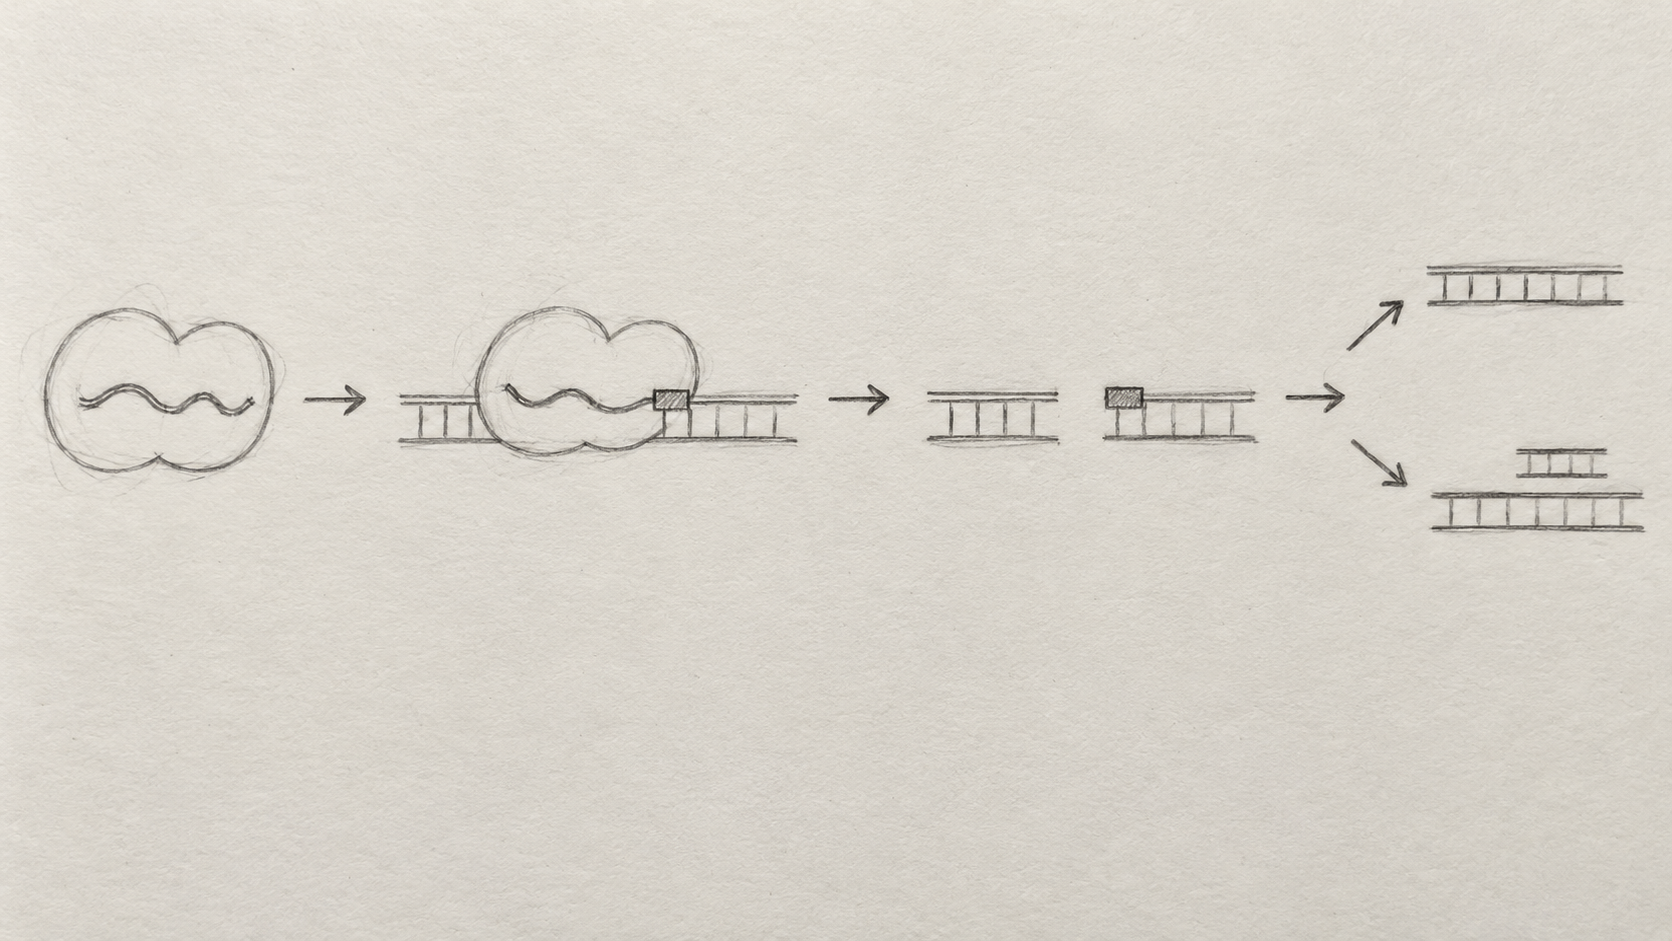
\includegraphics[width=\linewidth]{figures/ch03/ch03-02a-sketch-linear.png}};
\begin{scope}[x={(img.south east)},y={(img.north west)}]
  \node[font=\sffamily\bfseries\normalsize, anchor=north west, text=BookInk] at (0.04,0.94) {A};
\end{scope}
\end{tikzpicture}\\[1mm]
{\footnotesize A\quad Linear (left $\rightarrow$ right)}
\end{minipage}\hfill
\begin{minipage}[t]{0.32\linewidth}\centering
\begin{tikzpicture}
\node[anchor=south west,inner sep=0] (img) at (0,0) {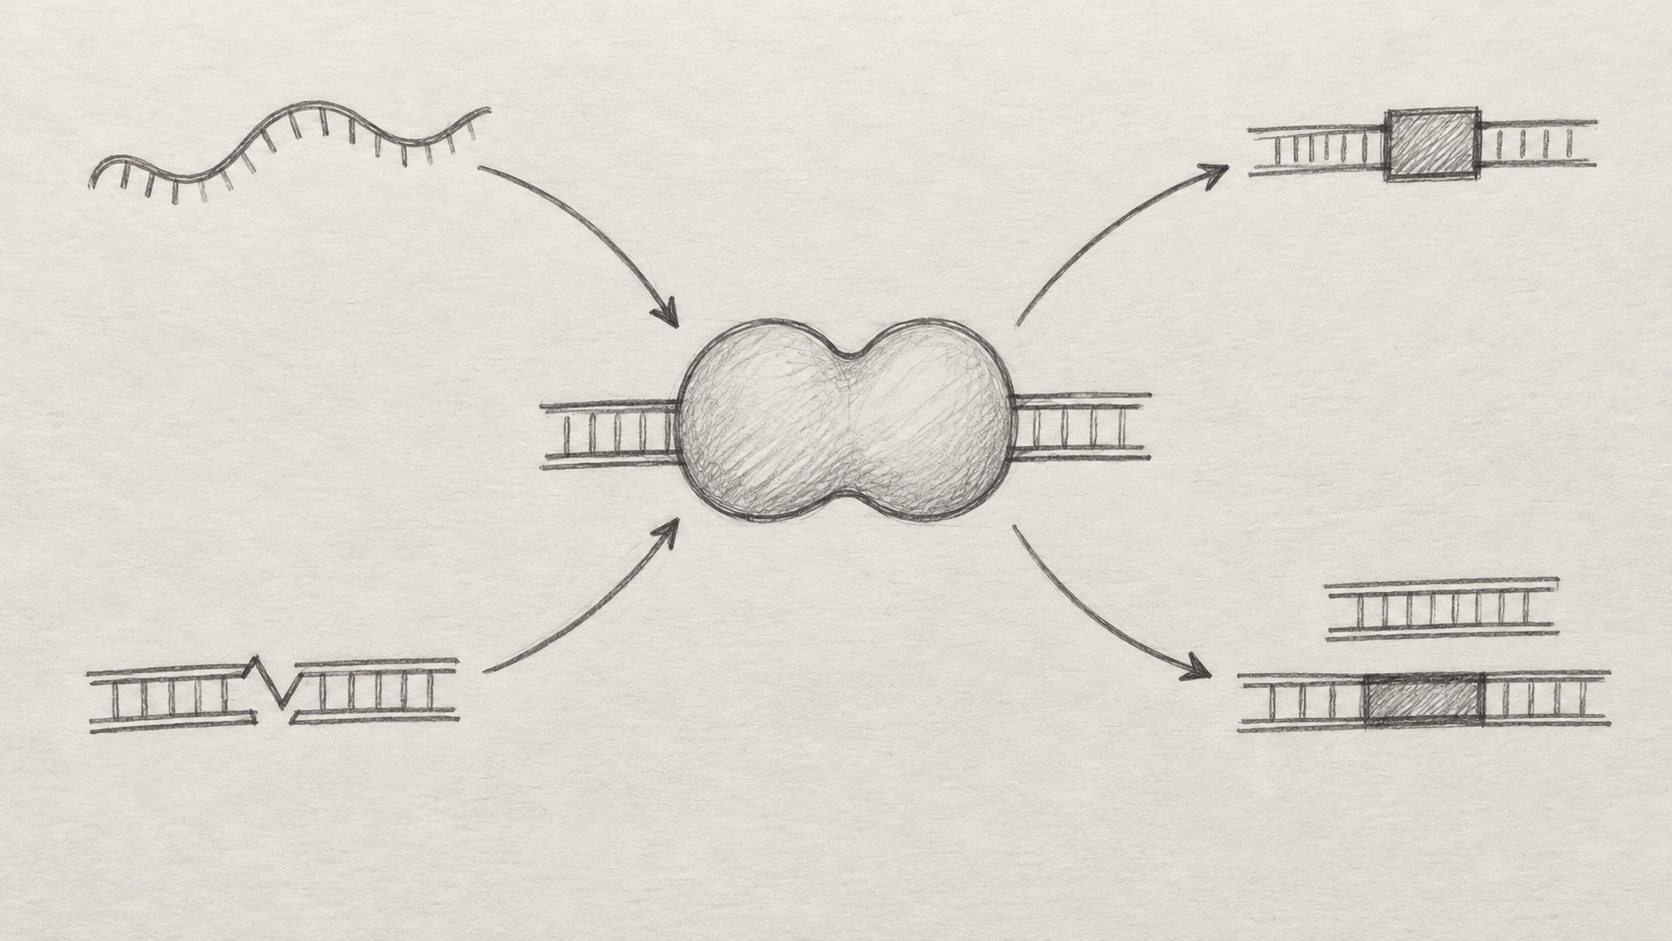
\includegraphics[width=\linewidth]{figures/ch03/ch03-02b-sketch-hub.png}};
\begin{scope}[x={(img.south east)},y={(img.north west)}]
  \node[font=\sffamily\bfseries\normalsize, anchor=north west, text=BookInk] at (0.04,0.94) {B};
\end{scope}
\end{tikzpicture}\\[1mm]
{\footnotesize B\quad Hub}
\end{minipage}\hfill
\begin{minipage}[t]{0.32\linewidth}\centering
\begin{tikzpicture}
\node[anchor=south west,inner sep=0] (img) at (0,0) {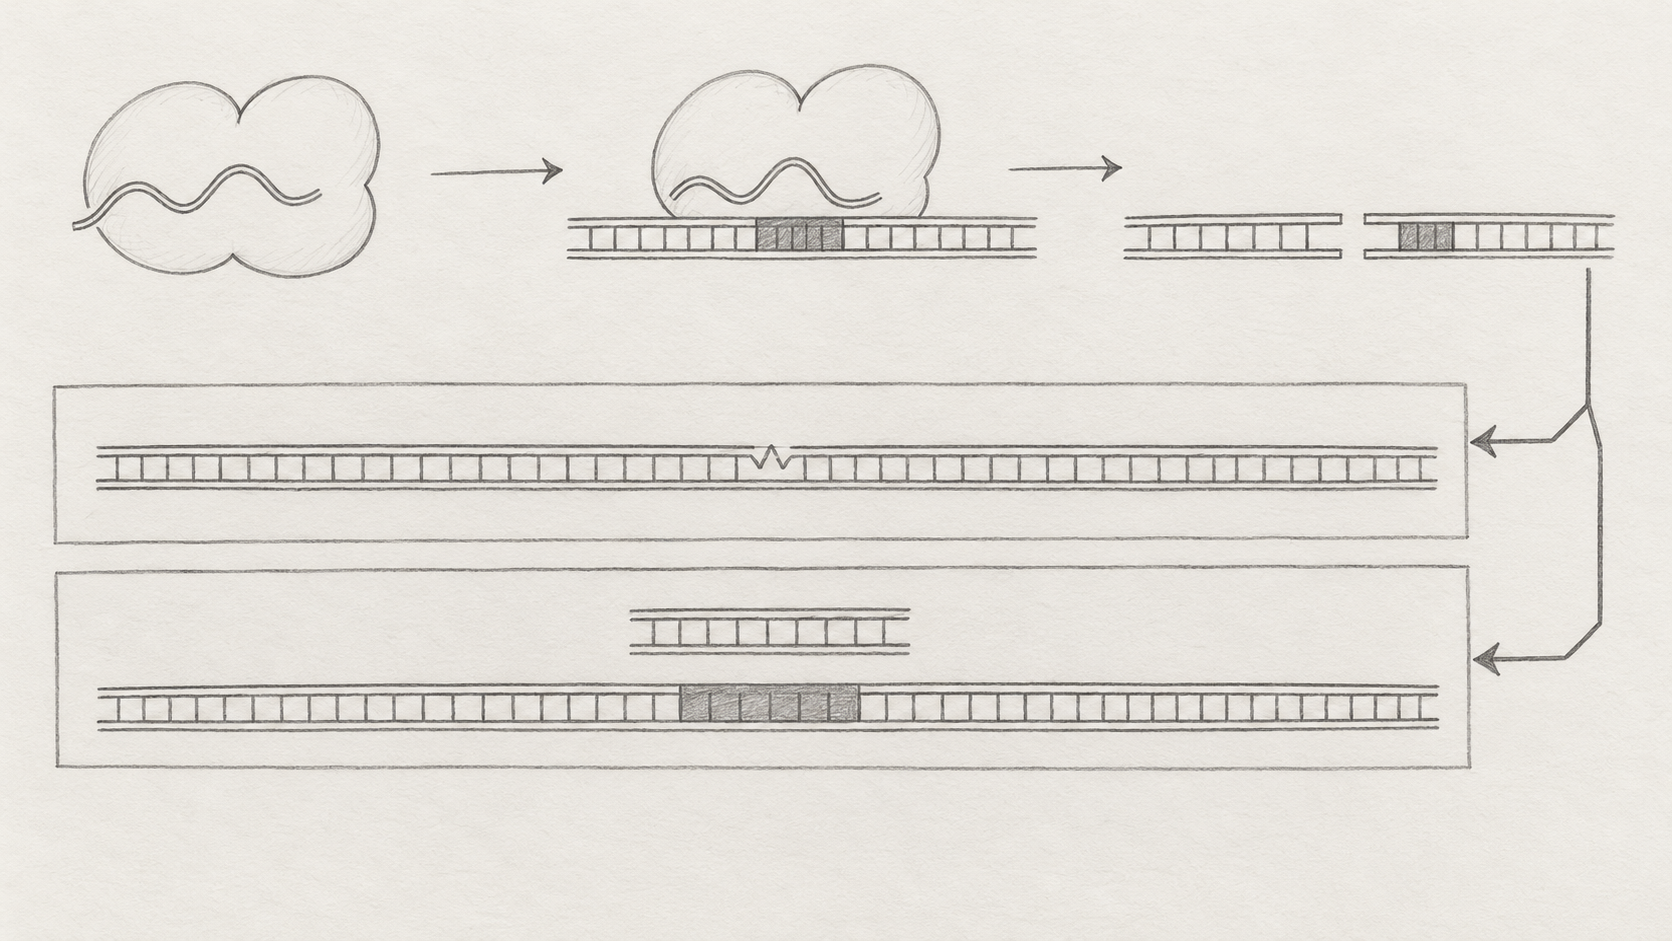
\includegraphics[width=\linewidth]{figures/ch03/ch03-02c-sketch-branch.png}};
\begin{scope}[x={(img.south east)},y={(img.north west)}]
  \node[font=\sffamily\bfseries\normalsize, anchor=north west, text=BookInk] at (0.04,0.94) {C};
\end{scope}
\end{tikzpicture}\\[1mm]
{\footnotesize C\quad Two-branch outcome}
\end{minipage}
\caption{Three layout skeletons for the same content (pencil sketches simulated with an image model). A sketch fixes regions, relative sizes, arrow directions, and white space, and carries no text; what each shape means is defined in the brief. A arranges the events in a single row, B centers on the Cas9--DNA complex, and C compresses the first three steps into a top row above two parallel repair lanes. The example figures in this chapter were generated with an image model; prompts and generation records are available in the book repository.}\label{fig:ch03-02}
\end{figure}

Inspecting the actual images and generation history of Figure~\ref{fig:ch03-02} yields three practical observations:

First, \textbf{a single-row linear layout succeeds on the first try, but squeezes the right-hand comparison region.} Figure~\ref{fig:ch03-02}A formed the four left-to-right stages and right-hand fork on the first sample, but because the first three steps take up most of the width, the two stacked outcome duplexes on the far right are compressed into very short segments.

Second, \textbf{a central hub layout inherently erases a unique entry point.} When generating Figure~\ref{fig:ch03-02}B, the first sample drew the bottom-left indel zigzag as a detached lightning bolt and pointed arrows inward from the right corners. The second sample restored the small zigzag attached to the DNA duplex, with single-headed arrows pointing inward from top-left and bottom-left and outward to top-right and bottom-right (with heavier pencil shading on the central protein), leaving no single entry point.

Third, \textbf{image models struggle with branched arrow routing into separate containers.} When generating Figure~\ref{fig:ch03-02}C, the first two samples drew the top row and the two lower pencil frames, but both times pointed \textbf{both branches of the split arrow onto the top edge of the upper frame}, leaving the lower lane without an entry arrow and splitting the upper DNA into a wide gap. Only on the third sample—after adding explicit routing instructions so the trunk runs down the right margin, sending one branch into the right end of the upper frame and the other into the right end of the lower frame, while keeping the upper DNA continuous around a small central zigzag—did the model connect both lanes properly. Even in Figure~\ref{fig:ch03-02}C, the two pencil boxes differ slightly in height (the lower box is taller) and the RNA inside the top-left protein has a double line. Sketching boxes and a split arrow by hand with a pencil takes a minute and avoids guessing topology through text.

Before moving on, check each sketch against four points: clear entry point, unambiguous fork into parallel outcomes, enough whitespace for labels, and zero text.

\section{From Sketches to Candidates, Then a Choice}

Next, we switch to \textbf{Sketch Mode} in the \scidraw{} prompt drawing tool (\sdtool{ai-drawing}), upload each sketch in turn, and paste the same English prompt derived from our brief. Changing only the uploaded sketch and the final layout line keeps visual style, color identities, step definitions, and exclusions identical for a fair test:

\begin{Prompt}
Flat 2D scientific overview schematic for a journal figure, landscape 16:9, pure white background. Clean vector illustration style: flat fills, thin dark gray outlines, no gradients, no shadows, no highlights, no 3D, no glow, no texture. ABSOLUTELY NO TEXT: no letters, no words, no numbers, no symbols, no labels, no legend, no title.
Follow the layout of the attached pencil sketch closely: same regions, same relative positions, same arrow directions.
OBJECTS (use these exact visual identities in every step where they appear):
- Cas9: a rounded two-lobed protein shape, muted blue-gray (#7C93A8).
- sgRNA: a single orange (#E69F00) strand with a short straight segment (the spacer) and a small hairpin loop scaffold, partly inside Cas9.
- Genomic DNA: two parallel dark gray (#4D4D4D) lines with short light gray rungs between them.
- PAM: a short bright yellow (#F0E442) segment on the upper DNA line.
- Double-strand break: a clean gap through both DNA lines, right next to the PAM.
- Donor template: a short separate double-stranded DNA; its two ends dark gray (homology arms), its middle segment teal (#009E73).
- NHEJ result: a continuous DNA with one small reddish-purple (#CC79A7) mark at the former break site.
- HDR result: a continuous DNA with a teal (#009E73) segment at the former break site, the same length as the donor's middle segment.
\end{Prompt}

\begin{Prompt}
STEPS: (1) Cas9 bound to sgRNA. (2) Cas9-sgRNA sitting on the DNA at the PAM, the orange spacer lying alongside the lower DNA line, the upper line slightly pushed away. (3) The DNA with the break next to the PAM, Cas9 lifted away. (4) Repair by end joining, giving the NHEJ result, with no donor. (5) Repair using the donor template, giving the HDR result; the donor appears only here. Steps are connected by solid dark gray arrows with filled heads; after step 3 the arrow splits into two equal arrows.
DO NOT DRAW: cells, nucleus, chromosomes, scissors, lightning, sparkles, double-helix twisting, realistic protein structure, any charts or data. Bottom 10% of the image empty.
LAYOUT [A]: one row of five steps left to right; steps 4 and 5 stacked at the right end.
LAYOUT [B]: radial; the DNA-bound Cas9 complex (step 2-3 merged) in the center, steps 1, 4, 5 and the PAM detail around it.
LAYOUT [C]: steps 1-3 as a compact row across the top third; below, two equal-height horizontal lanes stacked vertically, upper lane step 4, lower lane step 5, with the DNA in both lanes aligned at the same x positions and length.
\end{Prompt}

Keep one boundary in mind: \textbf{a sketch is a strong layout hint, not a pixel-level layout lock.} When rendering pencil lines into colored shapes, the model can still shift positions, duplicate markers, or swap object identities. After generation, we check each candidate against its sketch and overlay orange reading-order numbers (Figure~\ref{fig:ch03-03}).

\begin{figure}[htbp]\centering
\begin{minipage}[t]{0.32\linewidth}\centering
\begin{tikzpicture}[ord/.style={circle, draw=orange!85!black, line width=0.6pt, fill=orange!15, inner sep=1pt, font=\sffamily\bfseries\scriptsize, text=BookInk}]
\node[anchor=south west,inner sep=0] (img) at (0,0) {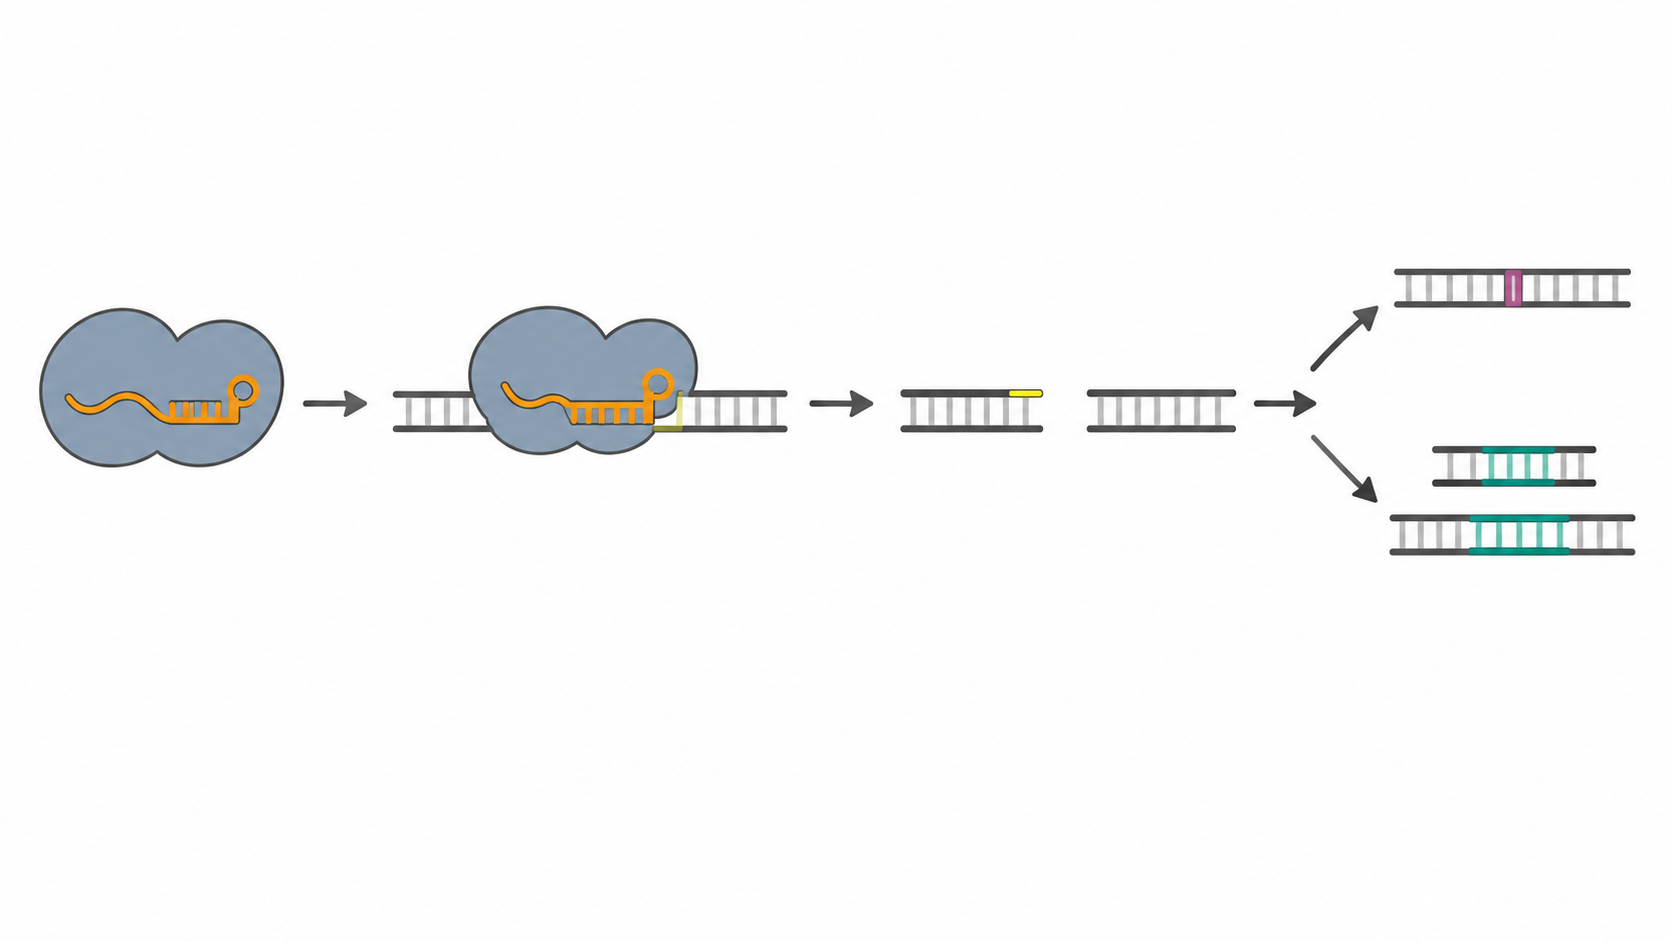
\includegraphics[width=\linewidth]{figures/ch03/ch03-03a-cand-linear.png}};
\begin{scope}[x={(img.south east)},y={(img.north west)}]
  \node[font=\sffamily\bfseries\normalsize, anchor=north west, text=BookInk] at (0.04,0.94) {A};
  \node[ord] at (0.08,0.55) {1};
  \node[ord] at (0.27,0.55) {2};
  \node[ord] at (0.46,0.55) {3};
  \node[ord] at (0.80,0.72) {4};
  \node[ord] at (0.80,0.35) {5};
\end{scope}
\end{tikzpicture}
\end{minipage}\hfill
\begin{minipage}[t]{0.32\linewidth}\centering
\begin{tikzpicture}[ord/.style={circle, draw=orange!85!black, line width=0.6pt, fill=orange!15, inner sep=1pt, font=\sffamily\bfseries\scriptsize, text=BookInk}]
\node[anchor=south west,inner sep=0] (img) at (0,0) {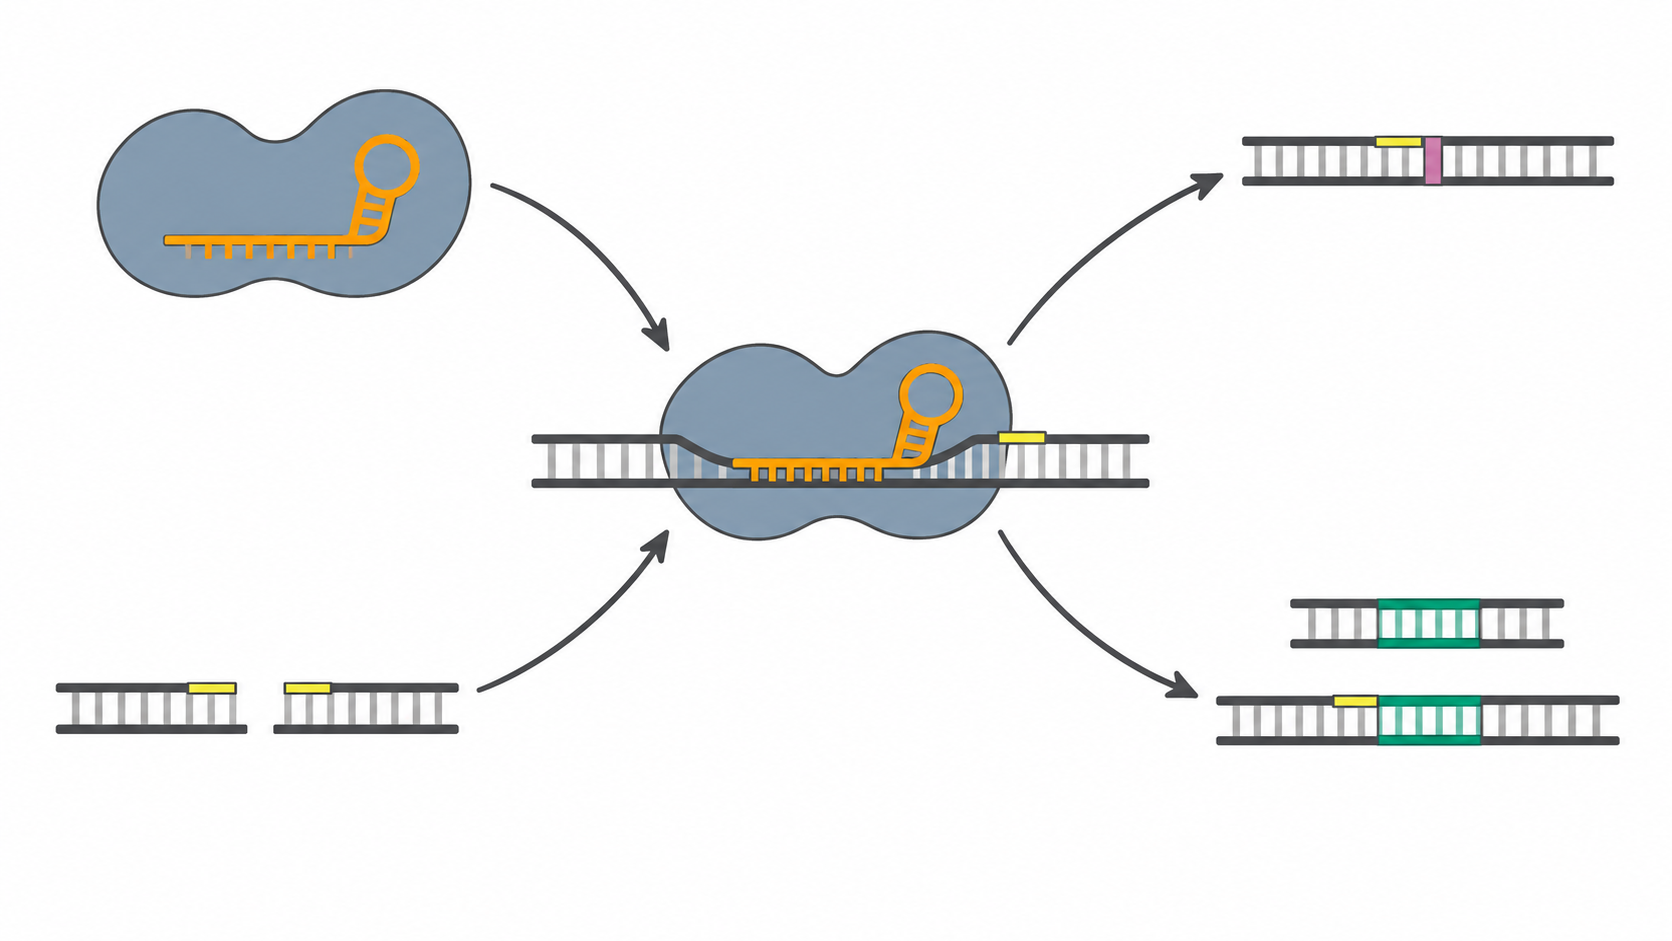
\includegraphics[width=\linewidth]{figures/ch03/ch03-03b-cand-hub.png}};
\begin{scope}[x={(img.south east)},y={(img.north west)}]
  \node[font=\sffamily\bfseries\normalsize, anchor=north west, text=BookInk] at (0.04,0.94) {B};
  \node[ord] at (0.50,0.52) {1?};
\end{scope}
\end{tikzpicture}
\end{minipage}\hfill
\begin{minipage}[t]{0.32\linewidth}\centering
\begin{tikzpicture}[ord/.style={circle, draw=orange!85!black, line width=0.6pt, fill=orange!15, inner sep=1pt, font=\sffamily\bfseries\scriptsize, text=BookInk}]
\node[anchor=south west,inner sep=0] (img) at (0,0) {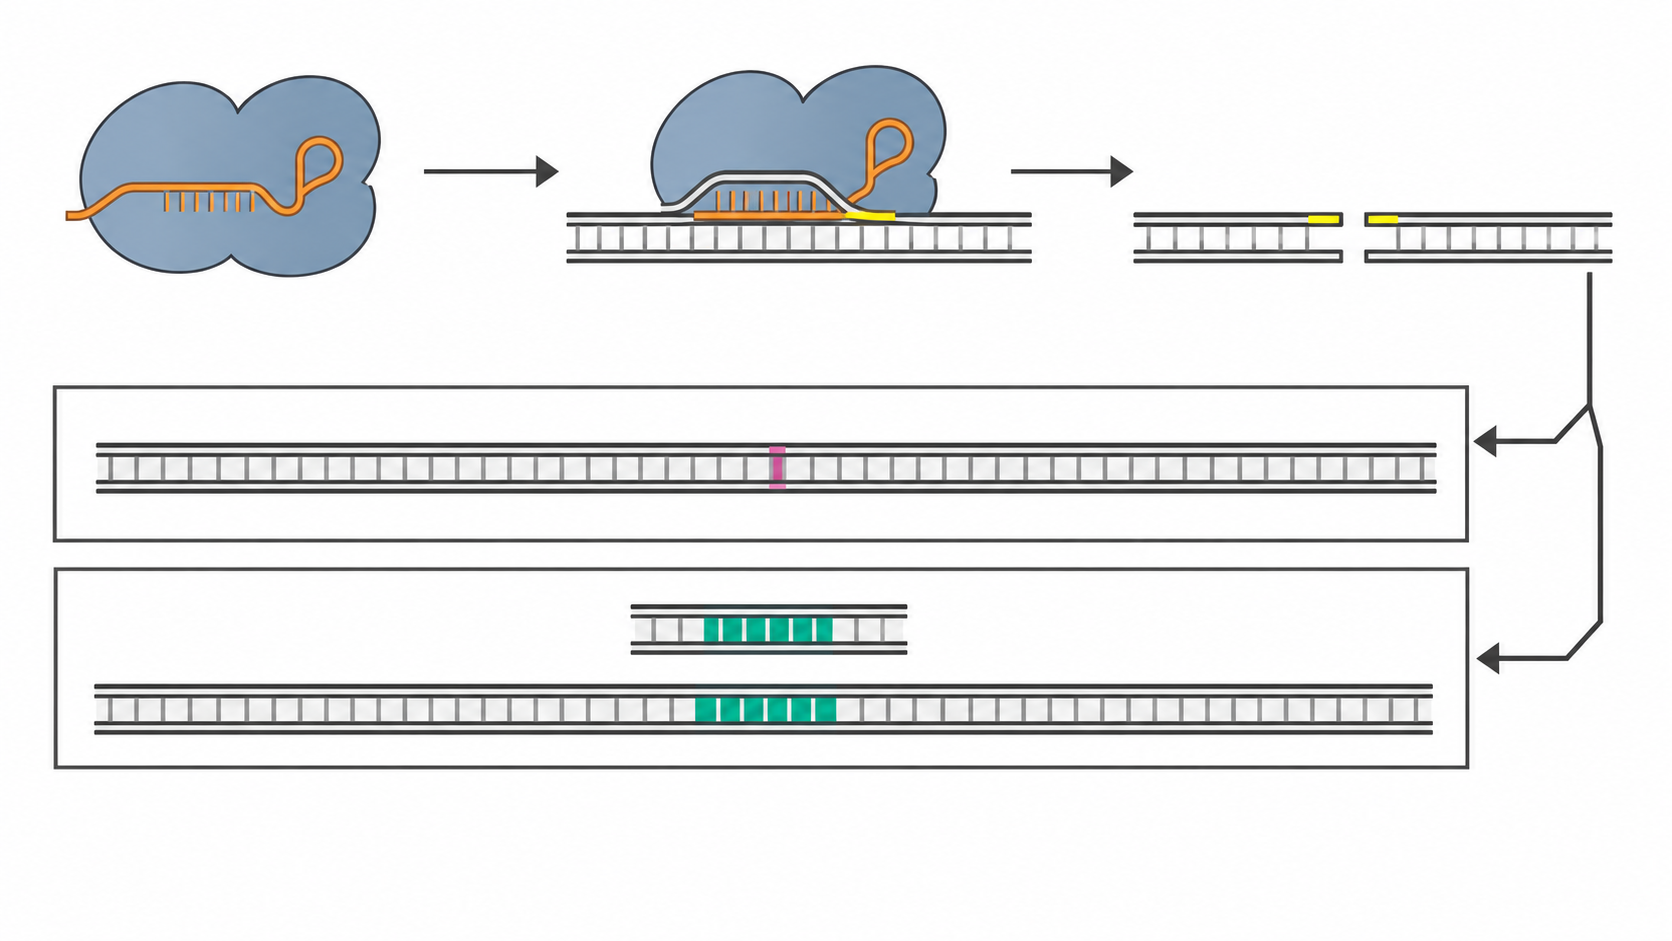
\includegraphics[width=\linewidth]{figures/ch03/ch03-03c-cand-branch.png}};
\begin{scope}[x={(img.south east)},y={(img.north west)}]
  \node[font=\sffamily\bfseries\normalsize, anchor=north west, text=BookInk] at (0.04,0.94) {C};
  \node[ord] at (0.15,0.85) {1};
  \node[ord] at (0.38,0.85) {2};
  \node[ord] at (0.62,0.85) {3};
  \node[ord] at (0.50,0.55) {4};
  \node[ord] at (0.50,0.22) {5};
\end{scope}
\end{tikzpicture}
\end{minipage}
\caption{Candidates generated from one brief and three different sketches. Orange numbers indicate the author's intended reading order (in an active project, test unnumbered prints with colleagues who have not seen the brief): in A and C the order is clear and matches the sequence of events; in B both top-left and bottom-left arrows point inward toward the center, leaving no unique entry point. Each candidate was checked against its input sketch for positional drift.}\label{fig:ch03-03}
\end{figure}

Comparing Figure~\ref{fig:ch03-02} and Figure~\ref{fig:ch03-03} side by side shows how each skeleton performed and where positional drift occurred:

\begin{itemize}
\item \textbf{Candidate A (Linear, Figure~\ref{fig:ch03-03}A):} Succeeded on the first sample in following Sketch A's single row, with accurate colors for Cas9 (blue-gray), sgRNA (orange), DNA (dark gray), PAM (yellow), indel (reddish-purple), and donor/insert (teal), placing the donor only at bottom right. However, Step 3 (cleavage) shows a classic \textbf{positional drift}: the PAM block on the \textbf{right} of the gap in Sketch A shifted to the \textbf{left} of the gap in Candidate A; R-loop pairing in Step 2 is also indistinct, the stacked outcomes on the right are cramped, and the donor's teal segment differs slightly in length from the HDR insert.
\item \textbf{Candidate B (Hub, Figure~\ref{fig:ch03-03}B):} Vividly shows how a flawed layout skeleton induces scientific errors. The first two samples reversed the bottom-left arrow outward (turning top-left into a pseudo-entry and expanding the lone sgRNA into a Cas9--sgRNA complex) or drew a double-headed arrow. After the third sample enforced two inward arrows from the left and two outward arrows to the right, arrow directions matched the sketch, but severe \textbf{identity swapping and marker proliferation} occurred: the NHEJ outcome (reddish-purple mark) moved from bottom-left to top-right while bottom-left became cleaved DNA; extra yellow PAM blocks appeared on both sides of the bottom-left gap, left of the top-right reddish-purple mark, and left of the bottom-right teal insert, while the central complex shows no clear break. Treating ``sgRNA,'' ``cleaved DNA,'' and ``repair outcomes'' as equal satellites also flattens the event hierarchy.
\item \textbf{Candidate C (Two-branch, Figure~\ref{fig:ch03-03}C):} Retained the ``compact three-step top row + right fork + stacked parallel lanes'' on the first sample; the short donor appears only in the lower HDR lane centered above the teal insert, the two long DNA strands align horizontally within 0.3\% of strand length, and no forbidden objects appear. Zooming in reveals two defects to fix: first, at Step 3 in the top row, \textbf{yellow PAM blocks appear on both the left and right sides of the gap} (duplicate PAM); second, the two rectangular lane frames differ in height, with the lower frame about 29\% taller than the upper frame (and all three candidates show slight shading/highlights on proteins and orange strands rather than purely flat fills).
\end{itemize}

In practice, show the unnumbered candidates to one or two colleagues who have not seen the brief and ask them to number steps 1--5 (a vision-capable conversational AI can offer a secondary check, but cannot replace human readers). Then evaluate the candidates with a criteria table (Table~\ref{tab:ch03-02-cmp} and Figure~\ref{fig:ch03-04}) rather than gut preference.

\begin{table}[htbp]\centering\footnotesize
\setlength{\tabcolsep}{3pt}
\renewcommand{\arraystretch}{1.15}
\caption{Comparison of the three candidate layout structures.}\label{tab:ch03-02-cmp}
\begin{tabularx}{\linewidth}{@{}>{\raggedright\arraybackslash}p{36mm}YYY@{}}
\toprule
\textbf{Criterion} & \textbf{A: Linear} & \textbf{B: Central Hub} & \textbf{C: Two-Branch} \\
\midrule
Single, unambiguous entry point & Yes (left Step 1) & No (two inward arrows from left corners) & Yes (top-left Step 1) \\
Reading direction matches event order & Yes & Partial (relies on arrows; objects swapped) & Yes \\
Outcomes directly comparable on shared baseline & No (stacked tightly at right end) & No (split between top-right and bottom-right) & Yes (stacked wide lanes, aligned endpoints) \\
Visual weight of main message (one break, two outcomes) & Low ($\approx$11\%--25\% at right) & Medium ($\approx$25\% in corners) & High ($\approx$50\% across lower half) \\
Label space at 174 mm width & Tight & Moderate & Generous \\
Best suited for & Stepwise slide animation & Non-sequential concept map & Journal overview figure \\
\bottomrule
\end{tabularx}
\end{table}

\begin{figure}[htbp]\centering
\resizebox{\linewidth}{!}{% FIG ch03-04 layout comparison (English)
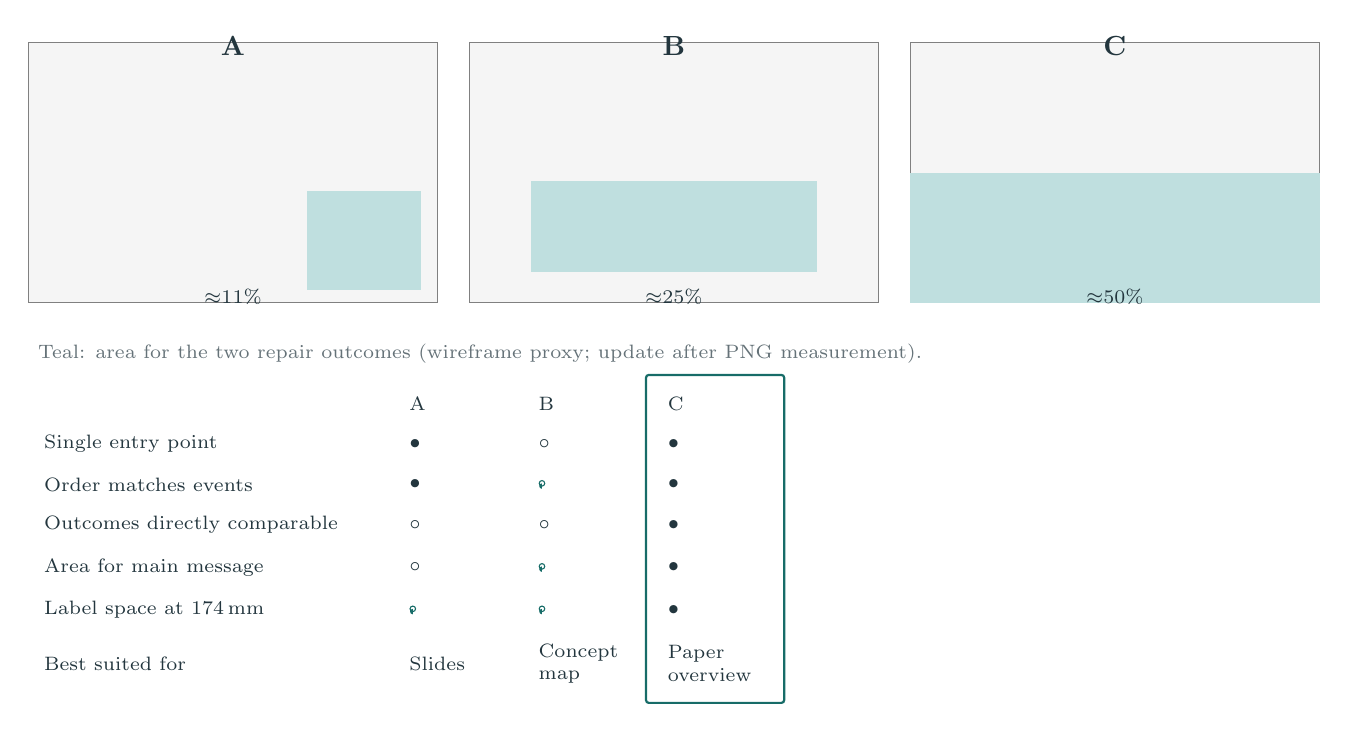
\begin{tikzpicture}[
  x=1mm, y=1mm,
  font=\sffamily\footnotesize,
  text=BookInk,
  wf/.style={draw=black!50, fill=black!4, line width=0.4pt},
  main/.style={fill=teal!25, draw=none},
]
  \def\fw{52}\def\fh{33}
  \begin{scope}[shift={(0,58)}]
    \draw[wf] (0,0) rectangle (\fw,\fh);
    \fill[main] (0.68*\fw,0.05*\fh) rectangle (0.96*\fw,0.43*\fh);
    \node[anchor=north, font=\bfseries] at (0.5*\fw,\fh+2) {A};
    \node[font=\scriptsize, anchor=south] at (0.5*\fw,-1.5) {$\approx$11\%};
  \end{scope}
  \begin{scope}[shift={(56,58)}]
    \draw[wf] (0,0) rectangle (\fw,\fh);
    \fill[main] (0.15*\fw,0.12*\fh) rectangle (0.85*\fw,0.47*\fh);
    \node[anchor=north, font=\bfseries] at (0.5*\fw,\fh+2) {B};
    \node[font=\scriptsize, anchor=south] at (0.5*\fw,-1.5) {$\approx$25\%};
  \end{scope}
  \begin{scope}[shift={(112,58)}]
    \draw[wf] (0,0) rectangle (\fw,\fh);
    \fill[main] (0,0) rectangle (\fw,0.50*\fh);
    \node[anchor=north, font=\bfseries] at (0.5*\fw,\fh+2) {C};
    \node[font=\scriptsize, anchor=south] at (0.5*\fw,-1.5) {$\approx$50\%};
  \end{scope}
  \node[font=\scriptsize, text=BookInk!70, anchor=north west] at (0,54)
    {Teal: area for the two repair outcomes (wireframe proxy; update after PNG measurement).};

  \matrix (m) [
    matrix of nodes,
    anchor=north west,
    row sep=1.8mm,
    column sep=3mm,
    nodes={font=\scriptsize, inner sep=2pt},
    column 1/.style={nodes={anchor=west}, text width=42mm},
    column 2/.style={nodes={anchor=center}, text width=12mm},
    column 3/.style={nodes={anchor=center}, text width=12mm},
    column 4/.style={nodes={anchor=center}, text width=12mm},
  ] at (0,48) {
    & {A} & {B} & {C} \\
    Single entry point & {$\bullet$} & {$\circ$} & {$\bullet$} \\
    Order matches events & {$\bullet$} & {\tikz[baseline=-0.6ex]{\fill[BookTeal] (0,0) arc (90:270:0.35); \draw[BookTeal] (0,0) circle (0.35);}} & {$\bullet$} \\
    Outcomes directly comparable & {$\circ$} & {$\circ$} & {$\bullet$} \\
    Area for main message & {$\circ$} & {\tikz[baseline=-0.6ex]{\fill[BookTeal] (0,0) arc (90:270:0.35); \draw[BookTeal] (0,0) circle (0.35);}} & {$\bullet$} \\
    Label space at 174\,mm & {\tikz[baseline=-0.6ex]{\fill[BookTeal] (0,0) arc (90:270:0.35); \draw[BookTeal] (0,0) circle (0.35);}} & {\tikz[baseline=-0.6ex]{\fill[BookTeal] (0,0) arc (90:270:0.35); \draw[BookTeal] (0,0) circle (0.35);}} & {$\bullet$} \\
    Best suited for & {Slides} & {Concept map} & {Paper overview} \\
  };
  \draw[BookTeal, line width=0.8pt, rounded corners=1pt]
    ([xshift=-2mm,yshift=2mm]m-1-4.north west) rectangle ([xshift=2mm,yshift=-2mm]m-7-4.south east);
\end{tikzpicture}
}
\caption{Comparing the three layouts against stated criteria. Top: in each wireframe, the teal area represents the proportion of layout space given to the two repair outcomes. Bottom: criterion-by-criterion assessment matrix. Layout C was chosen for the paper overview; A was kept for a stepwise slide version.}\label{fig:ch03-04}
\end{figure}

As Figure~\ref{fig:ch03-04} shows, because the core message is ``one break, two repair outcomes,'' Layout C devotes roughly 50\% of the canvas to the two aligned repair lanes so readers can directly compare the indel and precise edit at the same horizontal position. We record our rationale: \textbf{select C for the paper overview figure; retain A for stepwise presentation slides; discard B.}

\section{One Verifiable Goal per Revision}

When revising Candidate C, avoid bundled prompts such as ``fix the details, align the lanes, and make it cleaner.'' Reference-image editing in \scidraw{} (selecting a history image and entering an edit prompt) is conditional resampling, not vector translation; bundling multiple goals makes it impossible to tell which clause caused an unintended change.

Follow a strict revision discipline: \textbf{state only one verifiable goal per pass using ``target change + what stays unchanged + verification check,'' compare each output against the previous version by overlay, and log all unrequested changes.}

We first diagnose four checkpoints (1 to 4) on Candidate C (Figure~\ref{fig:ch03-05}, left):

\begin{itemize}
\item \textbf{Checkpoint 1 (PAM position):} Step 3 in the top row has yellow PAM blocks on both sides of the cleavage gap; we must \textbf{remove the left yellow block and keep only the upper-strand PAM immediately to the right of the gap}.
\item \textbf{Checkpoint 2 (Donor placement):} Although we worried the donor might float between lanes or duplicate, in Candidate C it already sits uniquely inside the lower HDR lane roughly centered over the edit. To test single-goal fine-tuning and center its teal middle segment strictly above the inserted segment, we still run one micro-adjustment pass.
\item \textbf{Checkpoint 3 (Lane alignment):} The two long DNA duplexes already align horizontally within 0.3\% ($<2\%$ target), but \textbf{the two rectangular lane frames differ in height by about 29\%} (lower frame taller than upper frame) and need equalizing.
\item \textbf{Checkpoint 4 (Extra background objects):} Prepared conditionally in case a cell nucleus or background shape appeared; Candidate C has a clean background, so \textbf{Revision 4 is skipped}.
\end{itemize}

The four single-goal revision prompts are:

\begin{Prompt}
[Revision 1 - PAM position] Edit the selected image. Change only one thing: move the small yellow PAM segment so that it sits directly next to the right side of the DNA gap at the cleavage step, on the upper strand, touching the gap. Keep every other object, color, line weight and position unchanged. Do not add any text.
\end{Prompt}

\begin{Prompt}
[Revision 2 - Donor placement] Edit the selected image. Change only one thing: move the short teal donor DNA so that it lies inside the lower repair lane only, directly above the DNA gap in that lane, horizontally centered on the gap. Remove any copy of the donor outside the lower lane. Keep everything else unchanged. No text.
\end{Prompt}

\begin{Prompt}
[Revision 3 - Lane alignment] Edit the selected image. Change only one thing: make the two repair lanes the same height, and draw the DNA in both lanes at the same horizontal position and the same length, so the two results line up vertically for comparison. Keep colors, objects and the top row unchanged. No text.
\end{Prompt}

\begin{Prompt}
[Revision 4 - Remove extra objects, conditional] Edit the selected image. Remove the cell nucleus outline and any background shapes. Change nothing else. No text.
\end{Prompt}

\begin{figure}[htbp]\centering
\begin{minipage}[t]{0.49\linewidth}\centering
\begin{tikzpicture}[font=\sffamily\footnotesize, text=BookInk]
  \node[inner sep=0, anchor=south west] (imga) at (0,0) {%
    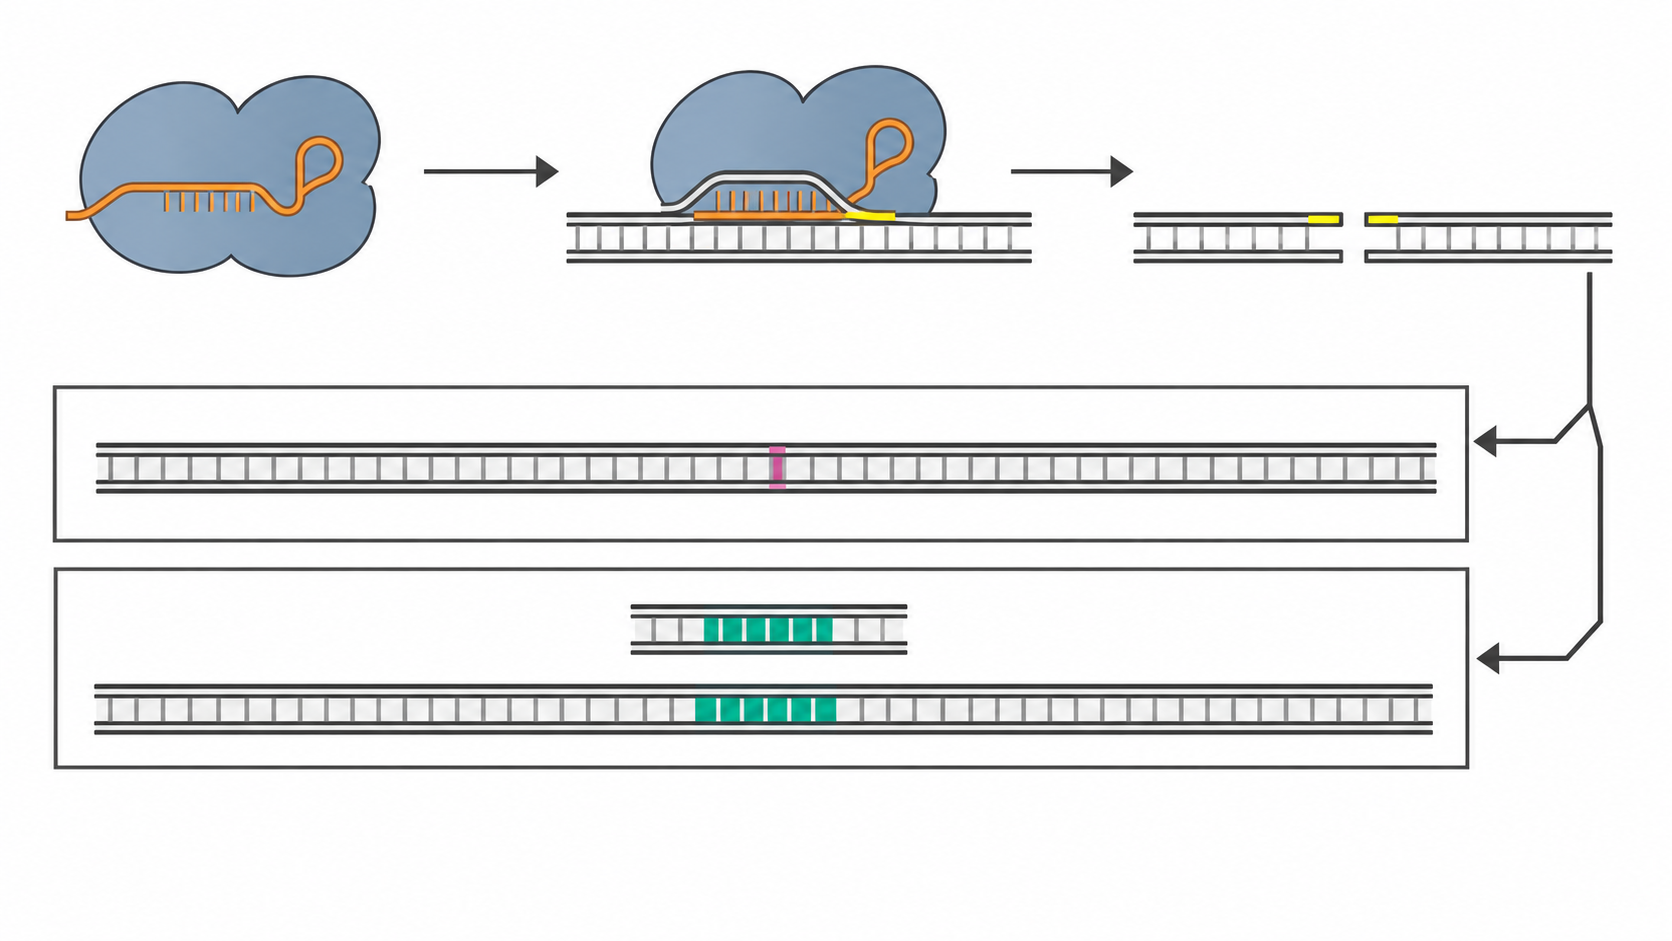
\includegraphics[width=\linewidth]{figures/ch03/ch03-03c-cand-branch.png}};
  \begin{scope}[x={(imga.south east)},y={(imga.north west)},
    issuemark/.style={circle, draw=red!75!black, line width=0.6pt, fill=white, fill opacity=0.88, text opacity=1, inner sep=0.8pt, font=\sffamily\bfseries\scriptsize, text=red!75!black}]
    \node[issuemark] at (0.62,0.78) {1};
    \node[issuemark] at (0.48,0.42) {2};
    \node[issuemark] at (0.72,0.28) {3};
    \node[issuemark] at (0.88,0.65) {4};
    \node[anchor=west, align=left, font=\sffamily\scriptsize] at (0.02,0.08) {%
      1 PAM position\quad 2 Donor placement\\
      3 Lanes misaligned\quad 4 Extra-object check};
  \end{scope}
\end{tikzpicture}
\end{minipage}\hfill
\begin{minipage}[t]{0.49\linewidth}\centering
\begin{tikzpicture}[font=\sffamily\footnotesize, text=BookInk]
  \node[inner sep=0, anchor=south west] (imgb) at (0,0) {%
    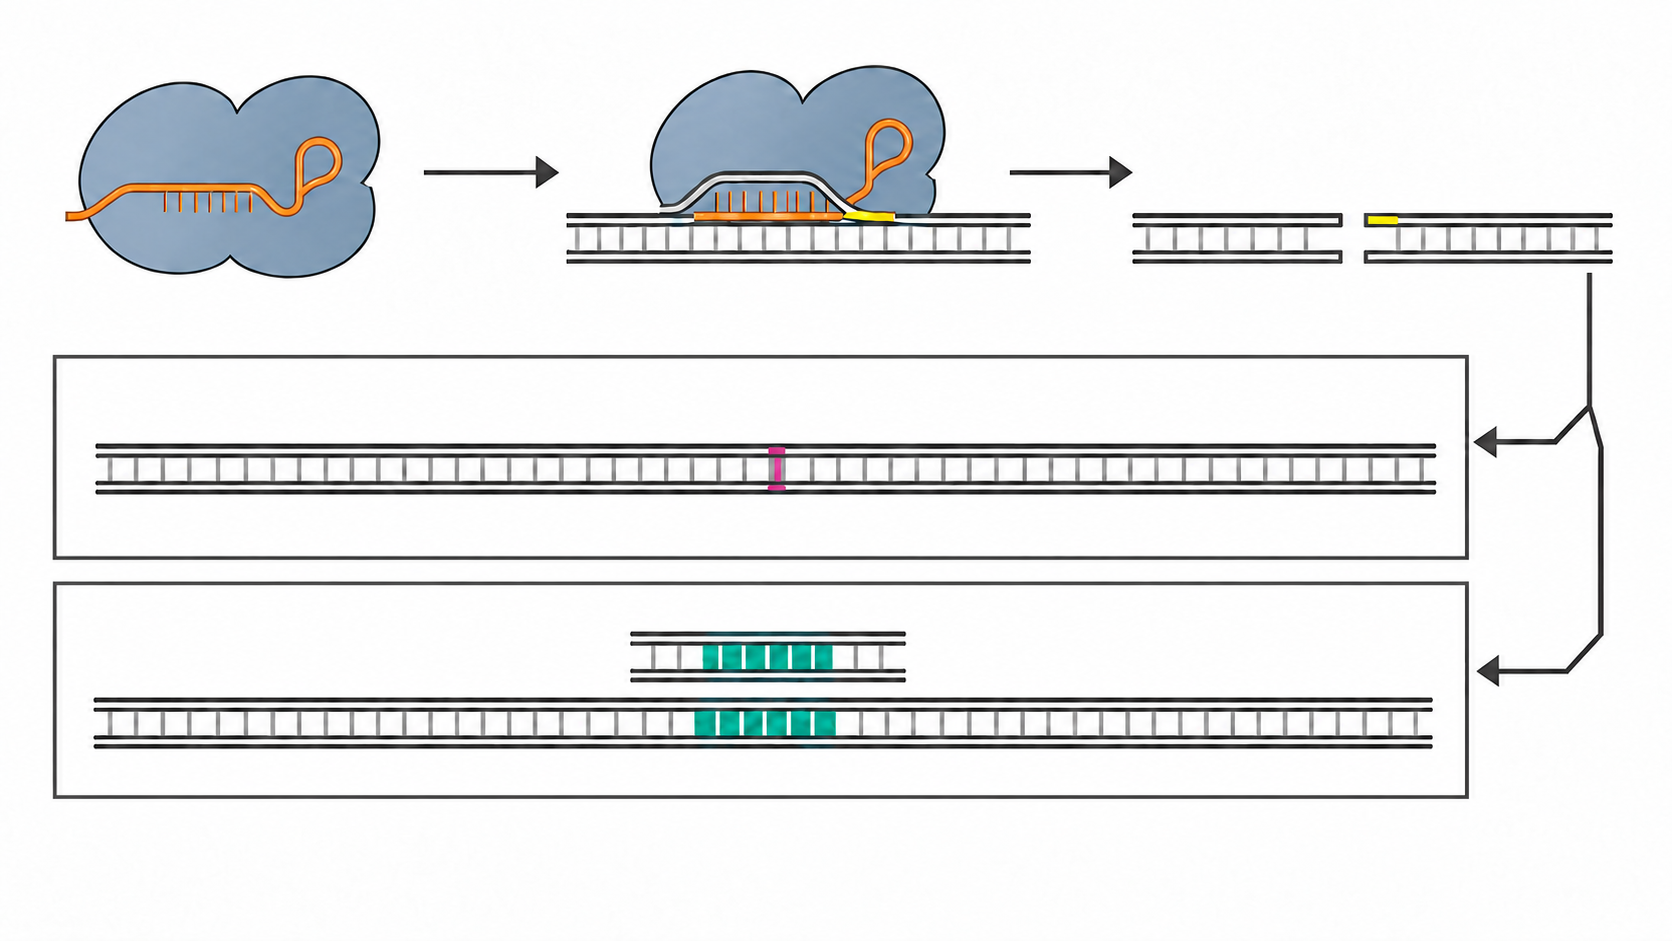
\includegraphics[width=\linewidth]{figures/ch03/ch03-05b-v3-revised.png}};
  \begin{scope}[x={(imgb.south east)},y={(imgb.north west)}]
    \draw[green!55!black, line width=0.8pt] (0.14,0.80) circle (0.07);
    \draw[green!55!black, line width=0.8pt] (0.48,0.29) circle (0.09);
    \node[anchor=west, align=left, font=\sffamily\tiny, text=green!45!black] at (0.02,0.08) {%
      Unrequested: sgRNA highlight redrawn,\\
      lower lane shifted \& $\sim$6\% frame gap};
  \end{scope}
\end{tikzpicture}
\end{minipage}
\caption{One change at a time. Left: four diagnostic checkpoints on Candidate C, where checkpoint 1 has duplicate yellow PAM blocks on both sides of the cleavage gap and checkpoint 3 has unequal lane frame heights (checkpoint 2 already has the donor inside the lower lane, and checkpoint 4 confirms no extra background objects). Right: the version after sequential single-goal edits; the duplicate left PAM is removed and the frame-height discrepancy is greatly reduced. Green circles mark minor unrequested redrawing and vertical shift recorded in the revision log.}\label{fig:ch03-05}
\end{figure}

Table~\ref{tab:ch03-03-log} records the seven actual edit calls from Candidate C to Figure~\ref{fig:ch03-05} (right) and how unrequested changes were handled:

\begin{table}[htbp]\centering\footnotesize
\setlength{\tabcolsep}{3pt}
\renewcommand{\arraystretch}{1.15}
\caption{Unrequested-change log from Candidate C to the revised draft.}\label{tab:ch03-03-log}
\begin{tabularx}{\linewidth}{@{}>{\raggedright\arraybackslash}p{25mm}ccY>{\raggedright\arraybackslash}p{22mm}@{}}
\toprule
\textbf{Revision Stage} & \textbf{Try} & \textbf{Goal Met?} & \textbf{Unrequested Changes (and Scientific Impact)} & \textbf{Decision} \\
\midrule
Rev 1: PAM position & 1 & No & Duplicate yellow PAM blocks remain on both sides of gap; minor line re-rendering (no scientific impact) & Revert to Candidate C \\
Rev 1: Explicit locus & 2 & \textbf{Yes} & Left duplicate PAM removed; subtle outline and texture re-rendering (no impact) & \textbf{Keep} as Baseline 1 \\
Rev 2: Donor centering & 1 & No & \textbf{Sole short donor duplex in lower lane deleted entirely (breaks scientific content)} & \textbf{Discard}; revert to Baseline 1 \\
Rev 2: Protect donor & 2 & \textbf{Yes} & Donor retained and centered over teal insert; donor shifted slightly downward (no impact) & \textbf{Keep} as Baseline 2 \\
Rev 3: Equal lane height & 1 & Partial & \textbf{Donor vanished; both outcome DNAs acquired both reddish-purple and teal marks (breaks science)} & \textbf{Discard}; revert to Baseline 2 \\
Rev 3: Protect identities & 2 & No & Scientific identities restored, but lower frame stretched taller and shifted down (geometry failed) & Discard; revert to Baseline 2 \\
Rev 3: Raise upper frame & 3 & \textbf{Yes} & Frame-height gap reduced from 29.4\% to 6.0\%, endpoint error 0.22\%; slight lower-lane shift and sgRNA highlight change (no impact) & \textbf{Keep} as Revised Draft \\
Rev 4: Remove background & 0 & --- & No cell nucleus or extraneous background shapes present & Conditionally skipped \\
\bottomrule
\end{tabularx}
\end{table}

Three practical rules emerge from Table~\ref{tab:ch03-03-log}:

\textbf{First, when an initial instruction fails, add explicit localization stating what is wrong, what to erase, and what to keep.} Try 1 of Revision 1 failed because a yellow PAM block already sat to the right of the gap, so the model left the extra left yellow block intact; specifying on Try 2 to ``erase the left yellow highlight back to dark-gray DNA and keep only the upper-strand yellow segment right of the gap'' worked immediately.

\textbf{Second, watch for destructive side effects—deleting a unique object or homogenizing contrasting outcomes—and revert immediately to the previous verified baseline.} On Try 1 of Revision 2, over-responding to ``Remove any copy'' erased the only donor template; on Try 1 of Revision 3, over-responding to ``same height and length'' deleted the donor and painted \emph{both} outcome duplexes with both reddish-purple and teal marks, destroying the NHEJ versus HDR comparison! Never patch a scientifically broken output; \textbf{step straight back to the previous verified baseline} and add protective constraints (e.g., keeping only the reddish-purple mark in the upper lane, keeping the teal insert and donor in the lower lane, and raising only the top edge of the upper frame).

\textbf{Third, separate scientific errors from harmless rendering drift, and switch to deterministic tools when needed.} The green circles in Figure~\ref{fig:ch03-05} (right) mark minor cumulative drift: slight changes in sgRNA highlight and stroke weight, a tiny downward shift of the lower lane, and a residual 6.0\% frame-height difference (down from 29.4\%, with DNA endpoints aligned within 0.22\%). Because these do not affect C1--C9, we log them and accept the draft. If a local edit still breaks key objects after three tries, stop resampling and draw exact geometry in TikZ.

\section{Closing the Case: Final Figure, Legend, and Verification}

To reserve space in the upper-right corner for the deterministic PAM inset (Figure~\ref{fig:ch03-07}), we run one final whitespace edit on Figure~\ref{fig:ch03-05} (right), shifting the top three steps leftward to clear the right 30\% of the upper row:

\begin{Prompt}
Edit the selected image. Change only one thing: shift the three steps of the top row to the left so that the right 30% of the top row is empty white space. Keep sizes, colors and the two lower lanes unchanged. No text.
\end{Prompt}

This step also took three samples: Sample 1 cleared only about 23\% width and detached Step 3 from the right-hand branch trunk; Sample 3 cleared ample space but routed the connector from Step 3 solely into the upper NHEJ box, breaking the ``one break feeding two pathways'' topology. We therefore chose \textbf{Sample 2} as our final text-free base image—the top three steps shift compactly left (with a slight unrequested scale reduction), the connector joins the shared right-hand fork cleanly, and the upper right offers an unobstructed zone about 30\% wide by 32\% high (crossed only along its bottom edge by the horizontal connector). Grayscale inspection confirms strong luminance contrast between the dark-outlined yellow PAM and the teal donor.

In LaTeX/TikZ, we then embed Figure~\ref{fig:ch03-07} into the upper-right whitespace using relative coordinates and overlay all English vector labels, step numbers 1--5, and the bottom legend to assemble the final figure (Figure~\ref{fig:ch03-06}).

\begin{figure}[htbp]\centering
\begin{tikzpicture}[font=\sffamily\scriptsize, text=BookInk]
  \node[anchor=south west, inner sep=0] (img) at (0,0) {%
    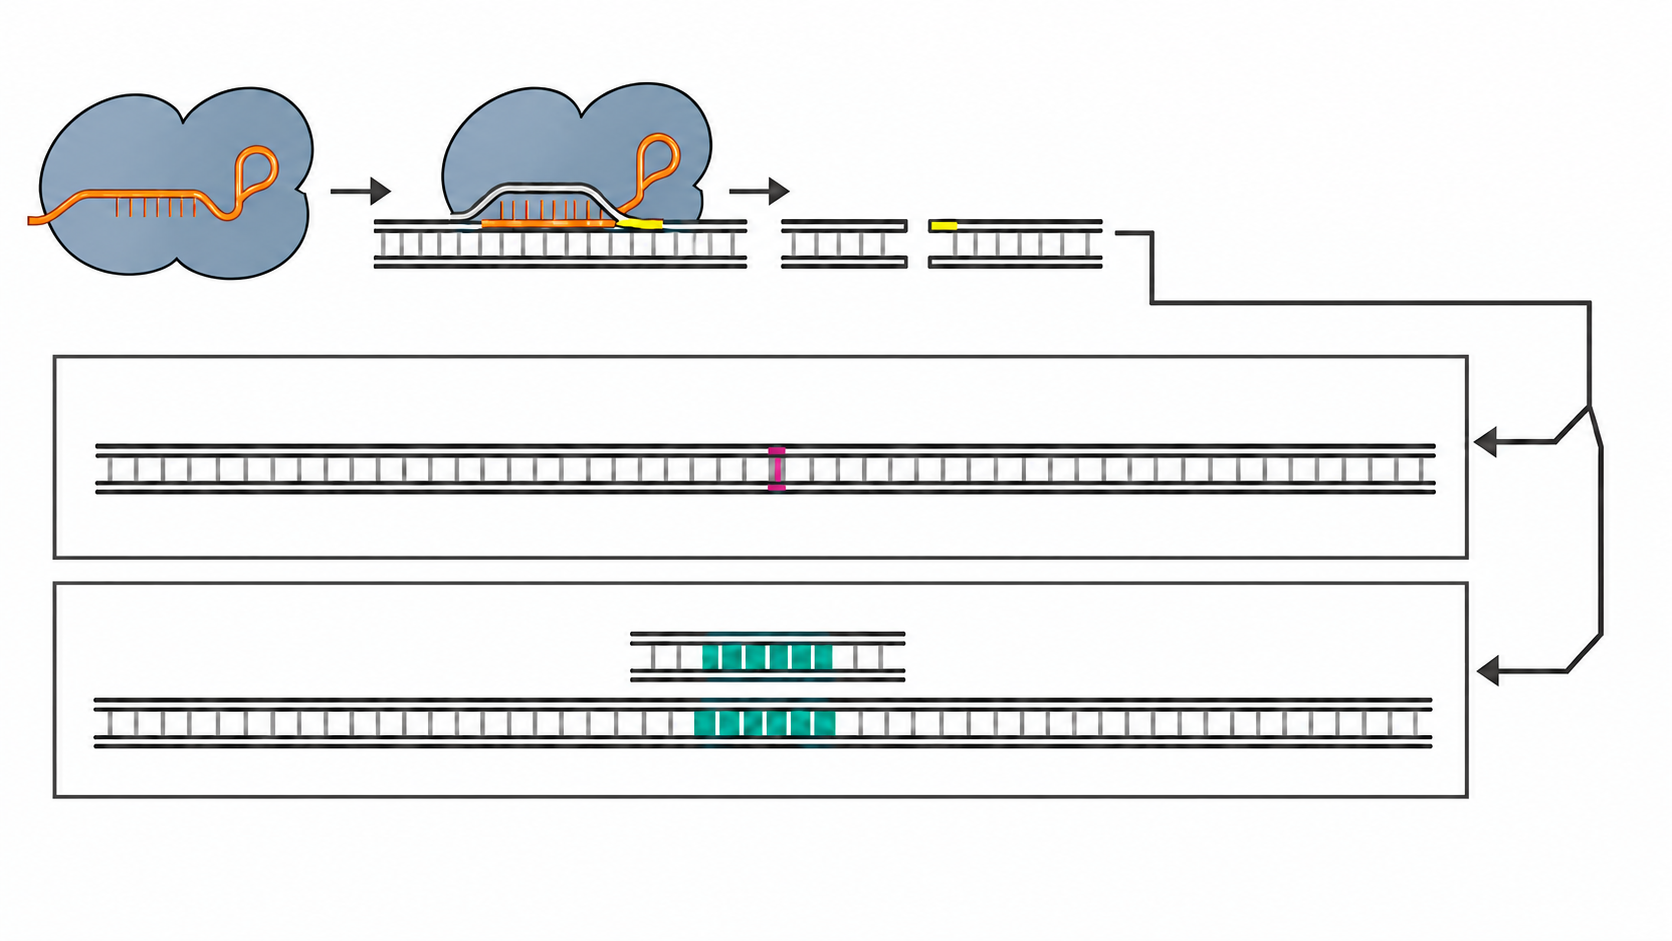
\includegraphics[width=\linewidth]{figures/ch03/ch03-06-final-base.png}};
  \begin{scope}[x={(img.south east)}, y={(img.north west)},
    lbl/.style={font=\sffamily\scriptsize, fill=white, fill opacity=0.88, text opacity=1, inner sep=1pt},
    ord/.style={circle, draw=orange!85!black, line width=0.5pt, fill=orange!15, inner sep=0.8pt, font=\sffamily\bfseries\tiny, text=BookInk}]
    \node[anchor=south west, inner sep=0, fill=white, fill opacity=0.92, text opacity=1] at (0.64,0.60) {%
      \resizebox{0.35\linewidth}{!}{% FIG ch03-07 PAM inset (English)
\begin{tikzpicture}[
  x=1mm, y=1mm,
  font=\sffamily\scriptsize,
  text=BookInk,
]
  \node[anchor=east] at (-2, 21.2) {Non-target strand};
  \node[anchor=east] at (-2, 7.2) {Target strand};
  \node at (6, 23.6) {5$'$};
  \node at (54.5, 23.6) {3$'$};
  \node at (55.5, 4.4) {5$'$};
  \node at (6, 4.4) {3$'$};

  \foreach \i in {0,...,19} {
    \pgfmathsetmacro{\x}{6+\i*2.4}
    \draw[draw=BookInk!50, fill=white] (\x,20) rectangle (\x+2.4,22.4);
  }
  \foreach \i in {0,1,2} {
    \pgfmathsetmacro{\x}{6+(17+\i)*2.4}
    \draw[draw=BookInk!50, fill=yellow!70] (\x,20) rectangle (\x+2.4,22.4);
  }
  \node[anchor=west, text=BookInk!80] at (6+17*2.4, 28.2) {PAM (NGG)};

  \foreach \i in {0,...,19} {
    \pgfmathsetmacro{\x}{6+\i*2.4}
    \draw[draw=BookInk!50, fill=white] (\x,6) rectangle (\x+2.4,8.4);
  }
  \foreach \i in {0,...,19} {
    \pgfmathsetmacro{\x}{6+\i*2.4}
    \draw[BookInk!35, thin] (\x+1.2,8.4) -- (\x+1.2,11.6);
    \draw[draw=orange!80!black, fill=orange!25, line width=1pt]
      (\x,4) rectangle (\x+2.4,6.4);
  }
  \draw[orange!80!black, line width=0.8pt]
    (6+19*2.4+2.4, 5) .. controls (6+21*2.4, 8) .. (6+21*2.4, 12)
    .. controls (6+21*2.4, 14) .. (6+19*2.4, 14);

  \node[anchor=west] at (6, 0.5) {sgRNA spacer};
  \pgfmathsetmacro{\cx}{6+16.5*2.4+1.2}
  \fill[black] (\cx,20) -- (\cx-0.8,21.2) -- (\cx+0.8,21.2) -- cycle;
  \fill[black] (\cx,6) -- (\cx-0.8,4.8) -- (\cx+0.8,4.8) -- cycle;
  \node[anchor=west] at (6+17.5*2.4, 13) {Cleavage site};
  \node[anchor=west, font=\scriptsize] at (6+16*2.4, 17) {RuvC};
  \node[anchor=west, font=\scriptsize] at (6+16*2.4, 3) {HNH};

  \draw[decorate, decoration={brace, amplitude=3pt}] (6, 15.5) -- (6+20*2.4, 15.5)
    node[midway, above=4pt] {$\sim$20 nt};
  \draw[decorate, decoration={brace, amplitude=2pt, mirror}] (6+16*2.4, 22.5) -- (6+17*2.4, 22.5)
    node[midway, below=2pt] {3 bp};
\end{tikzpicture}
}};
    \node[ord] at (0.04,0.92) {1};
    \node[ord] at (0.24,0.92) {2};
    \node[ord] at (0.46,0.82) {3};
    \node[ord] at (0.03,0.52) {4};
    \node[ord] at (0.03,0.22) {5};
    \node[lbl, font=\sffamily\bfseries\scriptsize] at (0.10,0.92) {Cas9};
    \node[lbl, font=\sffamily\bfseries\scriptsize] at (0.06,0.72) {sgRNA};
    \node[lbl] at (0.38,0.70) {PAM};
    \node[lbl] at (0.30,0.62) {Target DNA};
    \node[lbl] at (0.52,0.62) {Double-strand break};
    \node[lbl, anchor=west] at (0.06,0.48) {NHEJ (no template)};
    \node[lbl, anchor=west] at (0.06,0.22) {HDR (donor template)};
    \node[lbl] at (0.55,0.40) {Small indel};
    \node[lbl] at (0.50,0.34) {Donor template};
    \node[lbl] at (0.55,0.12) {Precise edit};
    \node[font=\sffamily\tiny, align=left, anchor=north west] at (0.02,0.04) {%
      Legend: solid arrow = step; split arrow = alternative repair routes; yellow = PAM; reddish-purple = indel; teal = donor-derived sequence};
  \end{scope}
\end{tikzpicture}
\caption{Final CRISPR--Cas9 genome editing overview figure. The text-free base image is combined with vector labels, a bottom legend bar, and the deterministic PAM detail inset (Figure~\ref{fig:ch03-07}) in the upper-right corner. The complete publication legend appears in the main text.}\label{fig:ch03-06}
\end{figure}

When drafting the figure legend—including with the \scidraw{} figure legend assistant (\sdtool{figure-legend})—verify every simplification statement and citation, and never invent efficiency percentages, sample sizes (\texttt{n=}), or statistical claims:

\begin{BookNote}
\textbf{Figure 1 | Overview of CRISPR--Cas9 genome editing and its two main repair outcomes.} A single guide RNA (sgRNA) binds Cas9. The complex recognizes a protospacer-adjacent motif (PAM; $5'$-NGG-$3'$ for SpCas9) in genomic DNA, the $\sim$20-nt spacer of the sgRNA base-pairs with the target strand, and Cas9 cleaves both strands about 3 bp upstream of the PAM, creating a double-strand break. The break can be repaired by non-homologous end joining (NHEJ), which needs no template and may leave small insertions or deletions (indels) that can disrupt a coding sequence; when a donor template with homology arms is supplied, homology-directed repair (HDR) can instead copy a precise change from the template. In most cell types HDR is less frequent than NHEJ. The inset shows the positions of the PAM, the target and non-target strands, and the cleavage site. For clarity, the three-dimensional structure of Cas9, the division of labor between the HNH and RuvC domains (except in the inset), repair factors, alternative end-joining pathways, off-target cleavage, and delivery methods are omitted. Based on Jinek et al.\ (2012), Doudna and Charpentier (2014), and Hsu et al.\ (2014).
\end{BookNote}

Finally, we verify Figure~\ref{fig:ch03-06} item by item against relationships C1--C9 (Table~\ref{tab:ch03-04-verify}).

\begin{table}[htbp]\centering\footnotesize
\setlength{\tabcolsep}{3pt}
\renewcommand{\arraystretch}{1.15}
\caption{Final verification record for the CRISPR--Cas9 overview figure.}\label{tab:ch03-04-verify}
\begin{tabularx}{\linewidth}{@{}l>{\raggedright\arraybackslash}p{22mm}>{\raggedright\arraybackslash}p{32mm}cY@{}}
\toprule
\textbf{\#} & \textbf{Relationship} & \textbf{Expected Visual Evidence} & \textbf{Status} & \textbf{Verification Notes} \\
\midrule
C1 & sgRNA--Cas9 binding & Both contact in Step 1 & Pass & Orange sgRNA contacts blue-gray Cas9; hairpin visible \\
C2 & PAM recognition & Complex at yellow PAM in Step 2 & Pass & Complex sits adjacent to bright-yellow PAM segment \\
C3 & Spacer--target pairing & RNA parallel to one strand, other displaced & Partial & Base image shows displaced arch, though rungs leave paired strand slightly schematic; clarified by upper-right TikZ inset \\
C4 & PAM position & Yellow block on non-target strand at $3'$ end & Pass & Base image keeps single right yellow block; inset locks exact $5'$-NGG-$3'$ polarity on non-target strand \\
C5 & Double-strand break & Both strands cut adjacent to PAM & Pass & Clean gap cuts both strands; $\sim$3 bp distance and HNH/RuvC assignment shown in inset \\
C6/C7 & NHEJ outcome & No template; reddish-purple indel mark & Pass & Upper lane 4 has no donor and a single central reddish-purple mark; legend uses ``may'' \\
C8/C9 & HDR outcome & Donor only here; DNA has teal insert & Partial & Lower lane 5 has sole short donor above teal insert (schematic length match) \\
--- & Reading order & Path 1--5 matches expected sequence & Pass & Top row 1--3 forks into lanes 4--5; DNA endpoint error 0.22\% (confirm with colleague blind test before submission) \\
--- & Exclusions & No nucleus, scissors, glow, or base text & Pass & 200\% zoom check confirms no baked-in text or forbidden objects \\
--- & Peer sign-off & Review by genome-editing colleague & Pending & Obtain colleague sign-off on inset strand polarity, HNH/RuvC labels, and legend phrasing before submission \\
\bottomrule
\end{tabularx}
\end{table}

Reviewing the workflow, the archived deliverables include: three sketches, three candidates with deviation notes, the comparison table and selection rationale, single-goal edit prompts and unrequested-change log, the deterministic inset, the text-free base image and final composite, the legend, and the verification record.

\section{What AI Can and Cannot Do at This Stage}

Table~\ref{tab:ch03-01} summarizes the boundaries between AI capabilities and author responsibilities during layout and sketch iteration.

\begin{table}[htbp]\centering\footnotesize
\setlength{\tabcolsep}{3pt}
\renewcommand{\arraystretch}{1.15}
\caption{What AI can do, what it cannot reliably do, and what the author must verify during layout and sketch development.}\label{tab:ch03-01}
\begin{tabularx}{\linewidth}{@{}>{\raggedright\arraybackslash}p{22mm}YYY@{}}
\toprule
\textbf{Sub-stage} & \textbf{What AI Can Do} & \textbf{What AI Cannot Do / Is Unreliable At} & \textbf{What the Author Must Verify} \\
\midrule
Proposing layout skeletons & Conversational AI can suggest verbal layout concepts and reading paths from a brief & Cannot judge which layout best fits the paper; \scidraw{} batch outputs share one prompt prior with limited structural variety & Draw at least one skeleton yourself; ensure all three skeletons differ in structure \\
Sketch $\rightarrow$ candidate figure & \scidraw{} Sketch Mode combines a sketch and prompt to quickly produce candidates following rough zones & A sketch is not a layout lock: objects may drift, merge, vanish, duplicate, or swap identities & Check each candidate against its sketch for position, direction, and count; log deviations \\
Evaluating reading order & A vision-capable conversational AI can describe where it would look first as an extra perspective & Model descriptions do not equal human eye paths and cannot replace peer testing & Have at least one colleague unfamiliar with the brief number the reading order \\
Choosing a layout & Can organize evaluation criteria into a comparison table & Cannot decide what the primary message of the figure should be & State the main message in the brief; record the selection rationale in the log \\
Iterative revision & Reference-image editing can adjust positions, delete objects, or resize frames per instruction & Local edits can cause collateral changes; outputs vary across runs; cannot enforce exact strand polarity or base distance & One goal per edit; overlay-compare with previous version; log unrequested changes; use TikZ for exact geometry \\
Scientific accuracy & Draws schematic relationships from prompts & Will not catch a PAM on the wrong strand, a distant cut site, or swapped NHEJ/HDR markers & Verify C1--C9 item by item; obtain domain-peer review \\
Text and labels & --- (base image must be text-free) & Generated text often misspells or misaligns terms & Overlay labels in LaTeX/TikZ and proofread spelling and positions \\
\bottomrule
\end{tabularx}
\end{table}

\section{Chapter Checklist}

\begin{itemize}
\item I can state the figure's entry point, path, and endpoint in one sentence.
\item The figure has only one visually heaviest element, and it carries the main message.
\item Objects grouped together (by proximity, alignment, or enclosure) are genuinely related; unrelated objects are not accidentally grouped.
\item At branch points, parallel options are drawn as parallel lanes so readers do not mistake them for sequential steps.
\item Details requiring exact geometry (strand polarity, position, base-pair distance) are drawn with deterministic tools or placed in an inset.
\item I drew and saved at least three structurally distinct sketches.
\item When generating candidates, I changed only the sketch while keeping the core brief text identical.
\item I checked each candidate against its sketch and logged positional deviations.
\item The reading order was tested by at least one person who had not seen the brief.
\item My layout choice is written as verifiable criteria rather than ``looks nicer.''
\item Every edit instruction has only one goal and states what must remain unchanged.
\item After each edit, I filled in the unrequested-change log and saved intermediate versions.
\item The final base image has no text; labels and legends are overlaid in LaTeX and checked for font size at final print width.
\end{itemize}

\section{Exercises}

\begin{enumerate}
\item \textbf{(Paper and pencil: Find the entry point of a figure)} Pick an overview figure or graphical abstract from a recent paper in your field. (a) Without reading the legend, look at the figure for 5 seconds and write down the first, second, and third elements you saw; (b) ask a classmate to do the same independently; (c) compare your sequences and identify which cues (size, contrast, position, arrows, numbering) caused agreement or divergence; (d) on a printout, sketch a better eye path and state which two elements should be moved.
\item \textbf{(Hands-on with \scidraw{}: One brief, three sketches)} Choose a process involving a branch or comparison (e.g., two failure modes of a material, or two branches of an algorithm). (a) Write a relationship table and drawing brief; (b) hand-draw linear, hub, and two-branch sketches and photograph them; (c) in \scidraw{} Sketch Mode, upload each sketch with the exact same brief text to generate candidates; (d) log deviations against the sketches and ask a classmate to number the reading order on all three; (e) score them with this chapter's comparison table and write your selection rationale. Submit: three sketches, three candidates, deviation log, and comparison table.
\item \textbf{(Revision discipline: From bundled feedback to single goals)} Here is a typical critique: ``Make the whole diagram cleaner, put the PAM in the right place, align the two outcomes, and make the colors more harmonious.'' (a) Split this into single-goal instructions, each stating what stays unchanged and how to check it; (b) point out which item should not be given to an image model, how to handle it instead, and why; (c) if you have candidates from Exercise 2, apply your instructions one by one, fill out the unrequested-change log, and count how many edits caused unrequested changes.
\end{enumerate}

\section*{References}

{\sloppy
\begin{itemize}
\item Chang HHY, Pannunzio NR, Adachi N, Lieber MR. Non-homologous DNA end joining and alternative pathways to double-strand break repair. \emph{Nature Reviews Molecular Cell Biology}. 2017;18(8):495--506. \path{doi:10.1038/nrm.2017.48}
\item Doudna JA, Charpentier E. The new frontier of genome engineering with CRISPR-Cas9. \emph{Science}. 2014;346(6213):1258096. \path{doi:10.1126/science.1258096}
\item Hsu PD, Lander ES, Zhang F. Development and applications of CRISPR-Cas9 for genome engineering. \emph{Cell}. 2014;157(6):1262--1278. \path{doi:10.1016/j.cell.2014.05.010}
\item Jinek M, Chylinski K, Fonfara I, Hauer M, Doudna JA, Charpentier E. A programmable dual-RNA--guided DNA endonuclease in adaptive bacterial immunity. \emph{Science}. 2012;337(6096):816--821. \path{doi:10.1126/science.1225829}
\item Nishimasu H, Ran FA, Hsu PD, Konermann S, Shehata SI, Dohmae N, Ishitani R, Zhang F, Nureki O. Crystal structure of Cas9 in complex with guide RNA and target DNA. \emph{Cell}. 2014;156(5):935--949. \path{doi:10.1016/j.cell.2014.02.001}
\item Ran FA, Hsu PD, Wright J, Agarwala V, Scott DA, Zhang F. Genome engineering using the CRISPR-Cas9 system. \emph{Nature Protocols}. 2013;8(11):2281--2308. \path{doi:10.1038/nprot.2013.143}
\item Rougier NP, Droettboom M, Bourne PE. Ten simple rules for better figures. \emph{PLoS Computational Biology}. 2014;10(9):e1003833. \path{doi:10.1371/journal.pcbi.1003833}
\item Wong B. Gestalt principles (Part 1). \emph{Nature Methods}. 2010a;7(11):863. \path{doi:10.1038/nmeth1110-863}
\item Wong B. Gestalt principles (Part 2). \emph{Nature Methods}. 2010b;7(12):941. \path{doi:10.1038/nmeth1210-941}
\item Wong B. Negative space. \emph{Nature Methods}. 2011b;8(1):5. \path{doi:10.1038/nmeth0111-5}
\item Wong B. Points of view: The overview figure. \emph{Nature Methods}. 2011c;8(5):365. \path{doi:10.1038/nmeth0511-365}
\item Wong B. Simplify to clarify. \emph{Nature Methods}. 2011d;8(8):611. \path{doi:10.1038/nmeth.1660}
\end{itemize}
\par}

\chapter{A Visual Language for the Whole Paper}

Maya Song, a doctoral candidate in oceanography, is preparing the final manuscript of a synthesis paper before submission. Drawing on four public observational and global carbon-budget datasets, the paper reviews how the global ocean absorbs the vast majority of excess heat in the climate system alongside roughly a quarter of anthropogenic carbon dioxide ($\text{CO}_2$) emissions. The manuscript contains four figures: Figure 1 is a conceptual schematic of the main pathways of air--sea heat and anthropogenic carbon uptake; Figure 2 presents long-term records of atmospheric $\text{CO}_2$ dry-air mole fraction at Mauna Loa Observatory, Hawaii, together with surface seawater partial pressure of $\text{CO}_2$ ($p\text{CO}_2$) and pH at Station ALOHA in the subtropical North Pacific; Figure 3 shows pentadal global ocean heat content anomalies in the $0\text{--}700\ \text{m}$ and $0\text{--}2000\ \text{m}$ layers; and Figure 4 tracks global anthropogenic $\text{CO}_2$ emissions and their partitioning among atmospheric growth, the ocean sink, and the land sink, paired with the ocean sink's share of total emissions.

Maya created these four figures over two months in separate work sessions: Figure 1 with an image generation tool, and Figures 2 through 4 on different days using separate scripts and conversational sessions. Viewed one at a time on a laptop screen, each plot looked passable. Just before submission, however, her advisor asked her to print all four figures side by side on a single A4 sheet (Figure~\ref{fig:ch04-01}). Seen together, the set fell apart at once---anticipating the exact critique a reviewer would later write: ``The figures are difficult to compare across the paper; colour assignments and symbol meanings contradict one another from one figure to the next.''

\begin{figure}[htbp]\centering
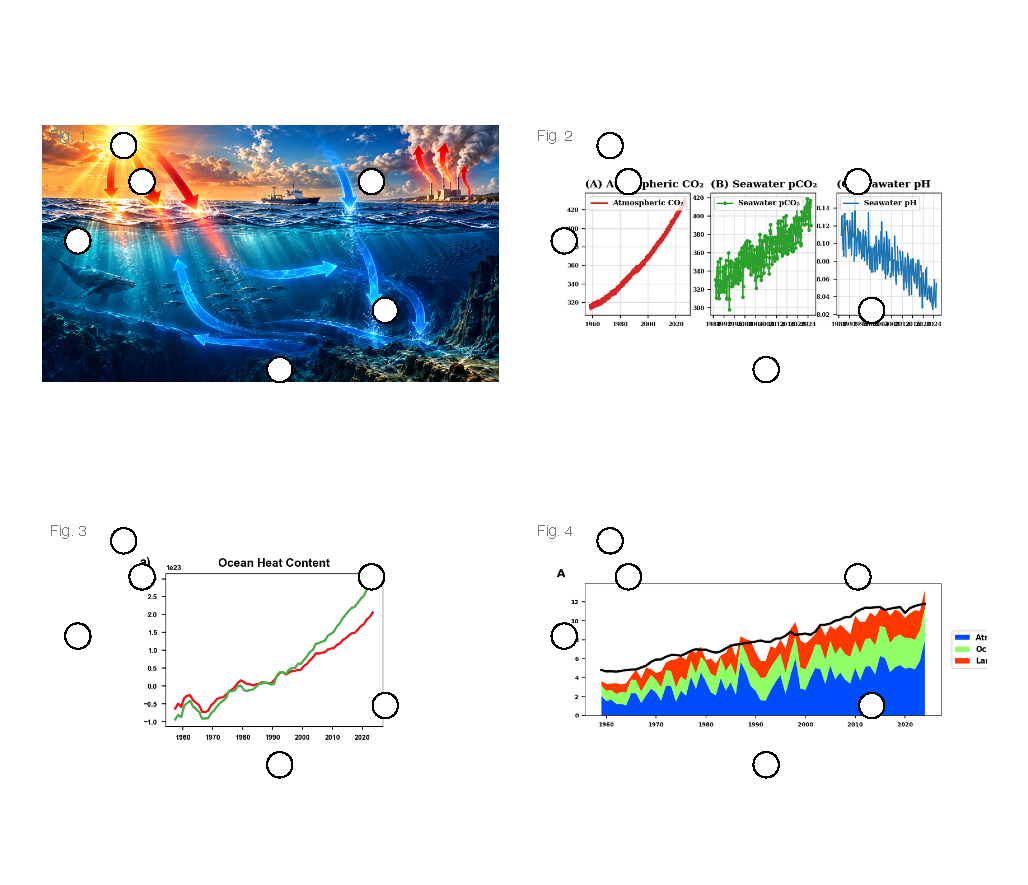
\includegraphics[width=\linewidth]{figures/ch04/ch04-01-inconsistent-set-en.pdf}
\caption{Four figures that each look acceptable in isolation but fail to work as a set (a deliberately inconsistent example). Six classes of conflict appear across the page: (1) red denotes solar radiation and smokestack emissions in Fig.\ 1, atmospheric $\text{CO}_2$ in Fig.\ 2, $0\text{--}700\ \text{m}$ ocean heat content in Fig.\ 3, and the land carbon sink in Fig.\ 4; (2) arrows of a single colour stand for unrelated processes in the schematic; (3) Fig.\ 3 relies solely on red versus green to separate two curves and omits a legend; (4) Fig.\ 4 uses a rainbow colormap for stacked areas while its legend box is clipped off the right edge; (5) the four figures mix three typefaces and four panel-labelling styles, and unconfigured Unicode characters produce missing-glyph boxes inside the callout circles and subplot titles; (6) the glossy 3D schematic introduces unmentioned decorative objects including a sun, a ship, a whale, and schools of fish. Figs.\ 2--4 plot real public data; only the styling differs.}\label{fig:ch04-01}
\end{figure}

Scanning across the four quadrants of Figure~\ref{fig:ch04-01} shows why an inconsistent figure set slows comprehension. In the top-left quadrant (Fig.\ 1), glowing red 3D arrows both shoot downward from the sun into the sea (solar heating) and rise from factory smokestacks into the sky (anthropogenic carbon emissions). In the top-right quadrant (Fig.\ 2a), a thick red curve denotes atmospheric $\text{CO}_2$. In the bottom-left quadrant (Fig.\ 3), the red curve switches meaning to $0\text{--}700\ \text{m}$ ocean heat content. In the bottom-right quadrant (Fig.\ 4), the red top band of the stacked area plot denotes the land carbon sink. Green shifts from surface seawater $p\text{CO}_2$ (Fig.\ 2b) to $0\text{--}2000\ \text{m}$ heat content (Fig.\ 3) to the ocean carbon sink (Fig.\ 4), while blue jumps from air--sea gas exchange and deep circulation arrows (Fig.\ 1) to seawater pH (Fig.\ 2c) to atmospheric $\text{CO}_2$ growth (Fig.\ 4). At each figure transition, the reader must unlearn the previous colour code and hunt for a legend to decode the new plot (Table~\ref{tab:ch04-diag}).

\begin{table}[htbp]\centering\footnotesize
\setlength{\tabcolsep}{3pt}
\renewcommand{\arraystretch}{1.15}
\caption{Diagnosis of the visual conflicts in the inconsistent first draft (Figure~\ref{fig:ch04-01}) and the cognitive cost imposed on the reader.}\label{tab:ch04-diag}
\begin{tabularx}{\linewidth}{@{}Y>{\raggedright\arraybackslash}p{18mm}Y@{}}
\toprule
\textbf{Visual conflict in the first draft} & \textbf{Location} & \textbf{Cognitive cost to the reader} \\
\midrule
Red, green, and blue switch meaning across figures (red denotes heat and emissions in Fig.\ 1, atmospheric $\text{CO}_2$ in Fig.\ 2, upper-ocean heat in Fig.\ 3, and the land sink in Fig.\ 4) & Figs.\ 1--4 & Readers cross-referencing panels mistakenly equate matching colours with the same physical quantity or carbon reservoir \\
Blue arrows represent both water circulation and air--sea carbon exchange; red arrows represent both solar heating and smokestack carbon emissions & Fig.\ 1 & Readers cannot tell from an arrow's geometry or hue which physical or biogeochemical process is depicted \\
Two curves of equal stroke width are distinguished solely by pure red versus pure green, with neither a legend nor direct labels & Fig.\ 3 & Readers with red--green colour vision deficiency cannot tell the $0\text{--}700\ \text{m}$ and $0\text{--}2000\ \text{m}$ layers apart \\
A \texttt{jet} rainbow stacked area plot represents the three carbon sinks, and omitting the budget imbalance causes the stacked top edge to cross above the black total-emissions line & Fig.\ 4 & The colour order has no physical meaning, sharp luminance jumps create false boundaries, and the sum of sinks appears to exceed total emissions \\
Three typefaces and four panel-label formats (\texttt{(A)}, \texttt{a)}, \texttt{A}, and none) are mixed, while Unicode subscripts and circled numbers render as missing-glyph boxes & Figs.\ 1--4 & The manuscript looks cobbled together; text references such as ``Fig.\ 3a'' or ``Fig.\ 2b'' are slow to locate \\
Type sizes range from $6\ \text{pt}$ to $12\ \text{pt}$, in-figure titles duplicate the captions, and the right-hand legend box is sliced off by the canvas edge & Figs.\ 2--4 & Visual hierarchy breaks down, plot area is wasted on redundant headers, and truncated labels (\texttt{Atr...}, \texttt{Oc...}, \texttt{La...}) leave series unidentified \\
A glossy 3D schematic clashes with flat 2D data plots and introduces a sun, a ship, a whale, and schools of fish & Fig.\ 1 & Unmentioned processes (solar radiation optics, shipboard surveys, marine food webs) distract from the paper's scope \\
Vertical-axis unit conventions vary, and multiplying values already in $10^{22}\ \text{J}$ by $10^{22}$ triggers a stray ``\texttt{1e23}'' offset label with no unit name & Figs.\ 2--4 & Readers must pause to reconcile orders of magnitude and infer missing physical dimensions \\
\bottomrule
\end{tabularx}
\end{table}

The figures in a paper are not standalone illustrations; they form a coordinated visual argument. Whenever multiple panels revisit the same physical quantities or reservoirs, choices of colour, typography, line weight, arrow geometry, and icon style constitute a paper-wide \textbf{visual language}. This chapter shows how to write a one-page visual specification before generating final figures, translate its clauses into style blocks for \scidraw{}, and audit every output so that all figures speak the same language.

\section{Colour Carries Meaning First}

When researchers choose colours for a figure, their first instinct is often aesthetic: picking a palette that looks pleasing on screen. In scientific figures, however, the primary role of colour is not decoration but \textbf{semantic encoding}. Readers automatically assume that a recurring, salient hue refers to the same variable or reservoir across a paper (Wong, 2010; Krzywinski, 2013). When colours are assigned ad hoc from default software cycles in separate sessions, cross-figure reasoning breaks down.

\textbf{First, assign semantic colours by scientific meaning and lock them across the manuscript.} Building a visual language starts with listing every core quantity or reservoir that recurs across your figures, assigning each role a dedicated hexadecimal colour (a semantic colour), and stating both what it \textit{is used for} and what it \textit{must never be used for}. In Maya's paper, the specification locks six quantitative roles and one schematic-only role:
\begin{itemize}
\item \textbf{Atmospheric carbon ($\text{CO}_2$):} Orange (\texttt{\#E69F00}), used for atmospheric $\text{CO}_2$ dots in Fig.\ 1, the Mauna Loa $\text{CO}_2$ curves in Fig.\ 2a, and atmospheric carbon growth in Fig.\ 4a. Never used for heat or oceanic variables.
\item \textbf{Ocean carbon:} Blue (\texttt{\#0072B2}), used for surface seawater dissolved inorganic carbon (DIC) in Fig.\ 1, seawater $p\text{CO}_2$ in Fig.\ 2b, the ocean carbon sink in Fig.\ 4a, and the ocean sink share in Fig.\ 4b. Never used for background water or heat.
\item \textbf{Land carbon:} Bluish green (\texttt{\#009E73}), reserved exclusively for the land carbon sink in Fig.\ 4a. Never used to colour phytoplankton icons in the schematic.
\item \textbf{Heat:} Vermilion (\texttt{\#D55E00}), used for heat-flux arrows in Fig.\ 1 and ocean heat content curves in Fig.\ 3. Never used for any carbon quantity.
\item \textbf{Seawater pH:} Reddish purple (\texttt{\#CC79A7}), dedicated solely to surface seawater pH in Fig.\ 2c.
\item \textbf{Anthropogenic emissions and carbon input fluxes:} Near-black dark gray (\texttt{\#3C3C3C}), used for total emissions in Fig.\ 4a and straight carbon-flux arrows in Fig.\ 1.
\item \textbf{Water-mass transport (schematic only):} Sky blue (\texttt{\#56B4E9}) as a broad semi-transparent band, reserved in Fig.\ 1 for sinking and interior water circulation; never used for data curves.
\end{itemize}

\textbf{Second, cap the number of semantic hues and separate variants of a single quantity using lightness tints of the same hue.} Visual working memory holds at most six or seven distinct colour categories without repeated trips back to a key (Wong, 2010). All structural elements---axes, reference lines, background zones, and icon bodies---must recede into neutral grays (\texttt{\#F2F2F2}, \texttt{\#BDBDBD}, \texttt{\#7A7A7A}). When a single panel compares two variants of the same physical quantity---such as $0\text{--}700\ \text{m}$ and $0\text{--}2000\ \text{m}$ ocean heat content anomalies in Fig.\ 3---do not borrow green or blue from the carbon budget. Instead, \textbf{keep the hue locked to vermilion for heat and separate depth layers by lightness}: plot $0\text{--}2000\ \text{m}$ in full-strength vermilion (\texttt{\#D55E00}) and $0\text{--}700\ \text{m}$ in a $55\%$ tint mixed $45\%$ toward white, labelling each curve directly at its right end (Figure~\ref{fig:ch04-02}, Figure~\ref{fig:ch04-03}). The reader sees immediately both that Fig.\ 3 represents ocean heat and which curve belongs to which depth layer.

\begin{figure}[htbp]\centering
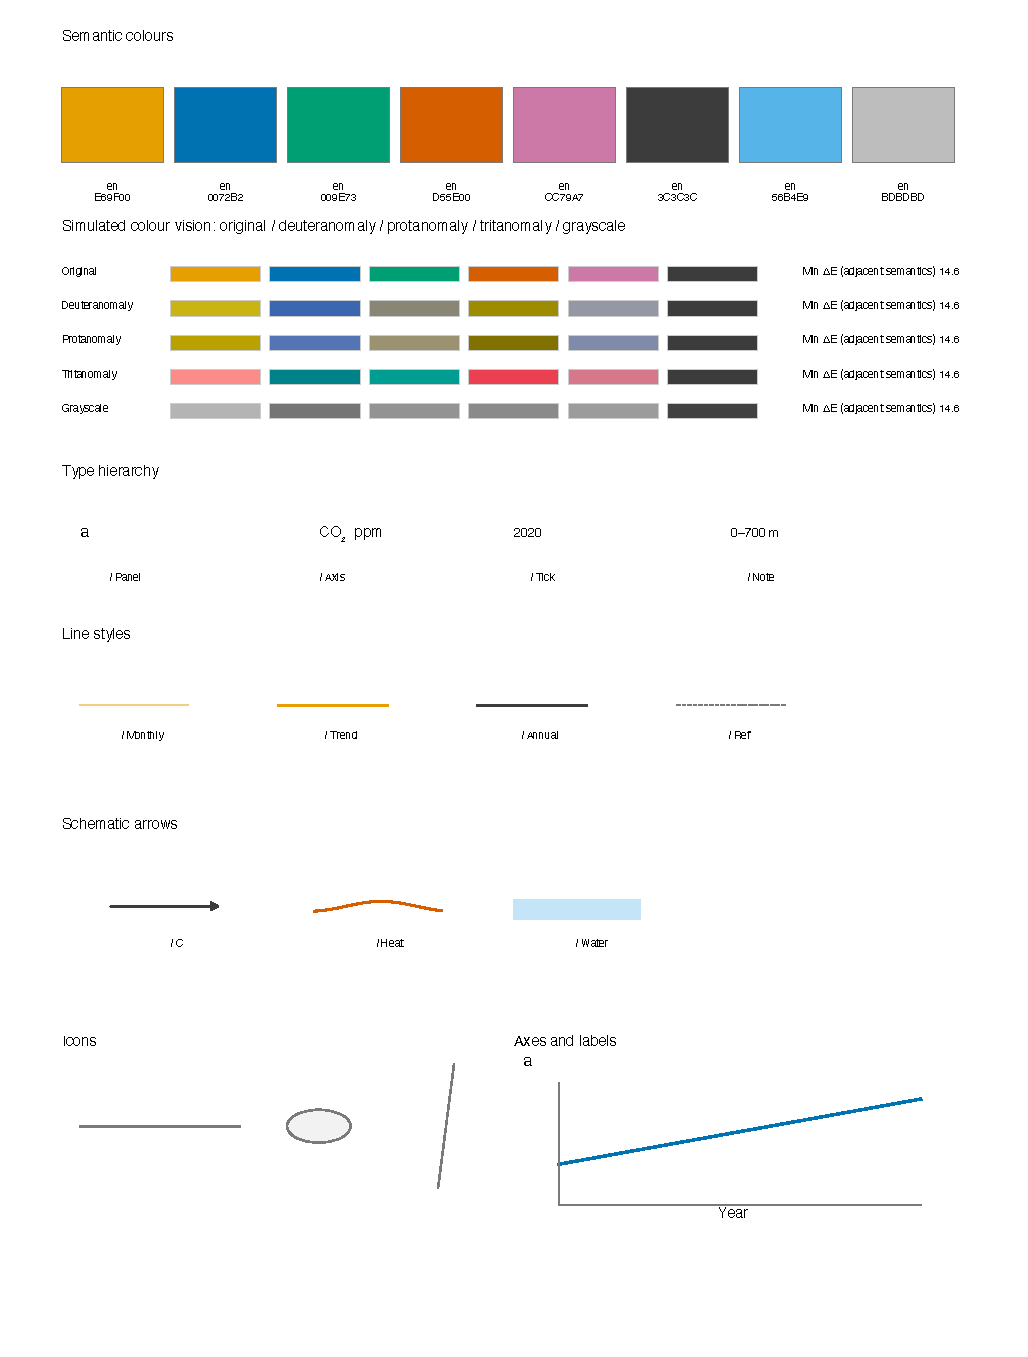
\includegraphics[width=0.95\linewidth,height=0.80\textheight,keepaspectratio]{figures/ch04/ch04-02-spec-page-en.pdf}
\caption{A one-page visual specification (v1) for the case-study manuscript. From top to bottom, the sheet defines semantic colour swatches, colour-vision deficiency (CVD) simulations and grayscale lightness strip, four-level type hierarchy at final print size, data-figure line styles, schematic process arrows, neutral icon style, and axis layout. The value at the right of each simulation row ($14.6$) is the smallest perceptual colour difference (CAM02-UCS $\Delta E$) between semantic colours that appear side by side in the same panel, computed by the script.}\label{fig:ch04-02}
\end{figure}

\textbf{Third, start from a colour-vision-accessible palette and never rely on red versus green alone.} Roughly $8\%$ of men of Northern European descent experience congenital red--green colour vision deficiency, most commonly deuteranomaly (Wong, 2011; note that a 2023 Author Correction to this article revised the cone sensitivity labels and terminology in the original figure). In the inconsistent draft of Fig.\ 3 (Figure~\ref{fig:ch04-01}), the two depth layers were plotted as equal-width lines in saturated red (\texttt{\#E41A1C}) and green (\texttt{\#4DAF4A}). Under simulated deuteranomaly (Figure~\ref{fig:ch04-03}, top right), those two curves collapse into nearly indistinguishable olive-brown lines. Begin instead from a colour-vision-accessible palette such as Okabe--Ito (Okabe and Ito, 2008; Wong, 2011) or ColorBrewer (Brewer).

\begin{figure}[htbp]\centering
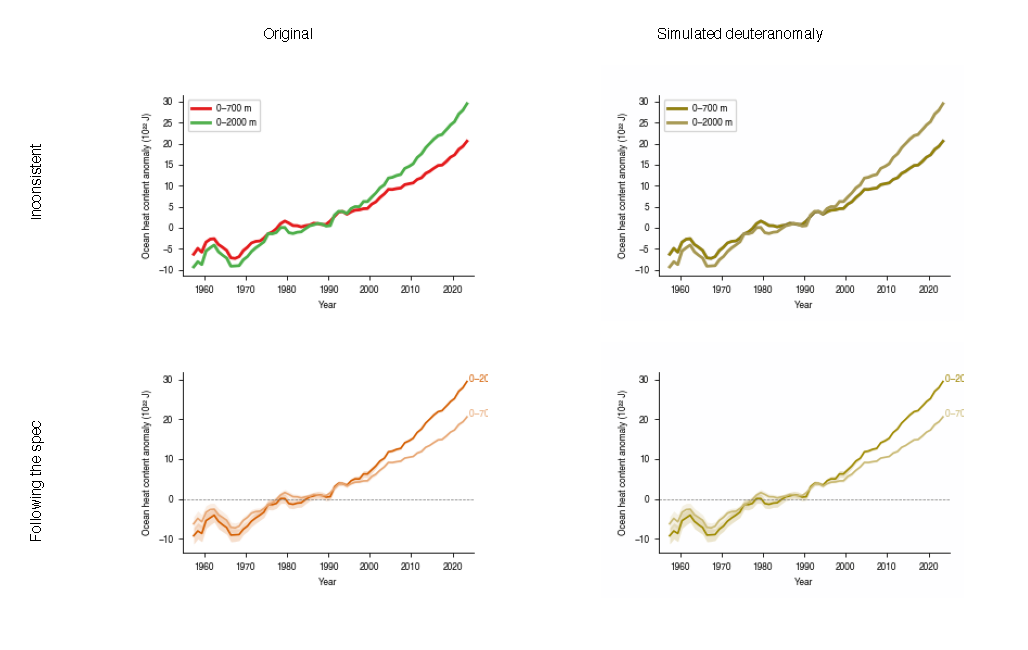
\includegraphics[width=\linewidth]{figures/ch04/ch04-03-cvd-check-en.pdf}
\caption{Two curves distinguished only by red and green become hard to tell apart under simulated deuteranomaly (top row); two lightnesses of one semantic hue paired with uncertainty bands and direct labels remain clearly separable (bottom row). The right column applies a full-image pixel simulation of deuteranomaly at severity $100$ using \texttt{colorspacious}. Data: NOAA NCEI pentadal global ocean heat content anomaly (Levitus et al., 2012).}\label{fig:ch04-03}
\end{figure}

\textbf{Fourth, combine colour-vision simulation and grayscale checks with redundant encoding.} Even an accessible palette needs quantitative verification when multiple curves share a panel. The second band of Figure~\ref{fig:ch04-02} simulates all eight swatches under deuteranomaly, protanomaly, and tritanomaly (at severity $100$ in \texttt{colorspacious}) and CIELAB lightness grayscale ($L^*$), reporting the minimum CAM02-UCS colour difference $\Delta E$ between semantic colours that appear side by side in the same panel. As a practical self-check guideline---offered here as an operational rule of thumb rather than a formal standard---\textbf{adjacent series in the same panel should maintain a CAM02-UCS distance of $\Delta E \ge 15$ under CVD simulation and a grayscale lightness difference of $\Delta L^* \ge 15$; whenever a pair falls near or below that threshold, add redundant encoding via line style, marker shape, or direct end-of-line labels.}

In Figure~\ref{fig:ch04-02}, the minimum adjacent distance across the simulation rows is $\Delta E = 14.6$---just shy of $15$---and in the grayscale row, ocean blue (\texttt{\#0072B2}), land bluish green (\texttt{\#009E73}), and heat vermilion (\texttt{\#D55E00}) sit at similar luminances. Thus no multi-hue palette can rely on hue alone. As the bottom row of Figure~\ref{fig:ch04-03} shows, pairing dark and light vermilion with $\pm 1\ \text{WOse}$ shading bands and right-end depth labels keeps the two curves distinct under severity-$100$ deuteranomaly simulation. Remember that numerical CVD simulation is only a colorimetric approximation; printing a black-and-white check sheet and asking a colleague with colour vision deficiency to review the figures remain essential before submission.

\textbf{Fifth, map continuous fields with perceptually uniform colormaps and retire rainbow colormaps.} Avoid rainbow colormaps such as \texttt{jet} when encoding continuous fields or stacked quantities. Because \texttt{jet} has a non-monotonic luminance profile, it creates false visual boundaries in cyan and yellow zones and fails under colour vision deficiency (Crameri et al., 2020). Use perceptually uniform sequential colormaps such as \texttt{viridis} or \texttt{cividis} (Nu\~nez et al., 2018) for single-ended variables, and zero-centered diverging colormaps for positive and negative anomalies.

\section{Type Hierarchy at Final Print Size}

A second source of visual incoherence in Figure~\ref{fig:ch04-01} is uncontrolled typography: Fig.\ 2 uses \texttt{DejaVu Serif} ($11\ \text{pt}$) with labels ``\texttt{(A)(B)(C)}''; Fig.\ 3 uses bold \texttt{Arial} ($9\ \text{pt}$) with ``\texttt{a)}''; and Fig.\ 4 uses \texttt{DejaVu Sans} ($8\ \text{pt}$) with ``\texttt{A}''. Because each plot was drawn on a different canvas size and scaled to fit the page, effective font sizes vary erratically across panels.

\textbf{First, lock the target journal's final print width before setting font sizes.} If you plot on a default $10 \times 6\ \text{inch}$ ($254 \times 152\ \text{mm}$) canvas and later shrink the figure into an $85\ \text{mm}$ single column, every font shrinks to one-third of its nominal size, turning a $10\ \text{pt}$ tick label into an illegible $3.3\ \text{pt}$ (Rougier et al., 2014; Wong, 2011 Typography). Always set physical canvas widths from the target journal's author instructions first---typically $85\text{--}89\ \text{mm}$ for single-column figures and $174\text{--}183\ \text{mm}$ for double-column figures ($174\ \text{mm}$ for Figs.\ 1, 2, and 4; $85\ \text{mm}$ for Fig.\ 3 in our case study)---specify font sizes in points at that exact width, and inspect the exported PDF at $100\%$ print scale.

\textbf{Second, establish a four-level type hierarchy in a single sans-serif family.} Govern all text across the manuscript with four levels (Figure~\ref{fig:ch04-02}, ``Type hierarchy''):
\begin{enumerate}
\item \textbf{Panel letters ($8\ \text{pt}$ bold):} Lowercase bold \textbf{a}, \textbf{b}, \textbf{c} without parentheses, placed outside the top-left corner of the axes frame.
\item \textbf{Axis labels ($7\ \text{pt}$ regular):} ``Quantity name (unit)'', such as ``Atmospheric $\text{CO}_2$ (ppm)''.
\item \textbf{Tick labels ($6\ \text{pt}$ regular):} Horizontal, unrotated, and non-overlapping.
\item \textbf{In-figure annotations and schematic labels ($6\text{--}7\ \text{pt}$ regular):} Direct curve labels and brief notes use $6\ \text{pt}$ regular (curve labels match the series colour); schematic region/object labels use $7\ \text{pt}$ and process labels use $6\ \text{pt}$.
\end{enumerate}

Use one sans-serif typeface (\texttt{Helvetica}, \texttt{Arial}, or \texttt{TeX Gyre Heros}) across all figures so small $6\text{--}7\ \text{pt}$ labels remain crisp (Wong, 2011 Typography). When producing bilingual editions, pair a uniform-stroke CJK gothic font (such as \texttt{FandolHei} or Source Han Sans) at the same point sizes while keeping numerals and units in the Latin sans-serif font.

Inspecting our rendered figures at $200\%$ zoom highlights a pervasive font-encoding trap. Look at the callout circles and Fig.\ 2 titles in Figure~\ref{fig:ch04-01}, the sample rows in Figure~\ref{fig:ch04-02}, and the vertical axis labels of Figure~\ref{fig:ch04-05} and Figure~\ref{fig:ch04-07}. When a script passes raw Unicode subscripts (such as the subscript $2$ in $\text{CO}_2$), Unicode superscript minus signs (in $\text{GtC yr}^{-1}$), circled numbers, or bilingual CJK strings directly to a font that lacks those glyphs, two failures occur: in raster or unconfigured font backends, missing characters render as empty missing-glyph boxes---visible inside the callout circles and Fig.\ 2 titles of Figure~\ref{fig:ch04-01} and the bilingual sample strings of Figure~\ref{fig:ch04-02} (such as ``\texttt{CO [box]ppm[box]}''); in vector PDF backends, missing glyphs can be silently dropped without warning---turning ``Atmospheric $\text{CO}_2$ (ppm)'' and ``Seawater $p\text{CO}_2$ ($\mu\text{atm}$)'' into ``Atmospheric CO (ppm)'' and ``Seawater pCO ($\mu$atm)'' in Figure~\ref{fig:ch04-05}, and turning ``$\text{GtC yr}^{-1}$'' into ``$\text{GtC yr}^{1}$'' in Figure~\ref{fig:ch04-07}. Meanwhile, a tuple-indexing bug in the specification script printed the language code ``\texttt{en}'' above each hex value in Figure~\ref{fig:ch04-02}. Never trust automatic font fallback for subscripts or exponents; use explicit math-mode or markup syntax (such as \texttt{\textbackslash textsubscript\{2\}} and \texttt{\$yr\^{}\{-1\}\$}) and check every exported PDF at $200\%$ zoom.

\textbf{Third, standardize unit notation, replace boxed legends with direct labels, and remove in-figure titles.} In Fig.\ 3 of Figure~\ref{fig:ch04-01}, multiplying values already reported in $10^{22}\ \text{J}$ by $10^{22}$ triggered a stray ``\texttt{1e23}'' offset label with no unit name. Our specification standardizes units into parenthetical SI form ($10^{22}\ \text{J}$, $\text{GtC yr}^{-1}$, $\mu\text{atm}$, ppm), deletes subplot titles that duplicate the caption, and replaces legend boxes with colour-matched labels at the right ends of the curves (Wong, 2011 Typography).

\section{One Meaning per Line and Arrow}

In the inconsistent draft (Figure~\ref{fig:ch04-01}), geometric primitives are equally muddled: Fig.\ 2a plots monthly means and deseasonalized trends as two heavy $2\ \text{pt}$ red curves on top of each other; Fig.\ 2b connects discrete cruise samples with straight green line segments; and Fig.\ 1 uses identical glowing arrows for gas exchange, solar heating, and ocean circulation. The core rule is straightforward: \textbf{one visual form per meaning, and one meaning per visual form.}

In data figures, series with different statistical meanings or sampling frequencies are separated by stroke weight, tint, marker geometry, and opacity (Table~\ref{tab:ch04-lines}):

\begin{table}[htbp]\centering\footnotesize
\setlength{\tabcolsep}{4pt}
\renewcommand{\arraystretch}{1.15}
\caption{Line, marker, and shading rules for the case-study data figures (Section C of the visual specification).}\label{tab:ch04-lines}
\begin{tabularx}{\linewidth}{@{}>{\raggedright\arraybackslash}p{36mm}Y>{\raggedright\arraybackslash}p{42mm}@{}}
\toprule
\textbf{Statistical nature of series} & \textbf{Specified visual encoding} & \textbf{Application in the case study} \\
\midrule
High-frequency raw observations (monthly means) & $0.5\ \text{pt}$ thin solid line in a $50\%$ lighter tint of the series semantic colour & Fig.\ 2a Mauna Loa monthly mean atmospheric $\text{CO}_2$ \\
Deseasonalized or running-mean trend & $1.2\ \text{pt}$ thick solid line in full-strength semantic colour & Fig.\ 2a deseasonalized $\text{CO}_2$, Fig.\ 3 pentadal heat content, Fig.\ 4b 10-year running mean \\
Discrete shipboard cruises or irregular sampling & Solid circular dots ($2.5\ \text{pt}$ diameter) with \textbf{no connecting line} & Fig.\ 2b surface seawater $p\text{CO}_2$, Fig.\ 2c surface pH, Fig.\ 4b annual sink share \\
Annual budget time series & $1.0\ \text{pt}$ solid line in the corresponding semantic colour & Fig.\ 4a annual emissions and the three carbon sinks \\
Uncertainty intervals (standard error or mean uncertainty) & $20\%$ opacity filled band in the series semantic colour, with no border line & Fig.\ 3 ($\pm 1\ \text{WOse}$ pentadal standard error), Fig.\ 4a (mean sink uncertainty bands) \\
Reference lines and station-change markers & $0.5\ \text{pt}$ dashed medium-dark gray (\texttt{\#7A7A7A}) line with $6\ \text{pt}$ gray text note & Fig.\ 2a Maunakea eruption relocation line, Fig.\ 3 zero-anomaly baseline \\
\bottomrule
\end{tabularx}
\end{table}

For example, Mauna Loa monthly means summarize continuous daily measurements, so plotting them as a $0.5\ \text{pt}$ light-orange line beneath a $1.2\ \text{pt}$ full-orange deseasonalized curve preserves the seasonal cycle while highlighting the long-term trend. Station ALOHA measurements, by contrast, come from discrete research cruises with irregular spacing and occasional gaps; connecting them with straight lines falsely implies linear interpolation between voyages, so they must be plotted as unlinked dots.

In the conceptual schematic (Fig.\ 1), we likewise assign four mutually exclusive arrow geometries to the four physical and biogeochemical processes (Table~\ref{tab:ch04-arrows}):

\begin{table}[htbp]\centering\footnotesize
\setlength{\tabcolsep}{4pt}
\renewcommand{\arraystretch}{1.15}
\caption{Process arrow rules for the case-study schematic (Section D of the visual specification).}\label{tab:ch04-arrows}
\begin{tabularx}{\linewidth}{@{}>{\raggedright\arraybackslash}p{36mm}Y>{\raggedright\arraybackslash}p{44mm}@{}}
\toprule
\textbf{Physical or biogeochemical process} & \textbf{Specified geometry and colour} & \textbf{Dual redundancy of shape and colour} \\
\midrule
Carbon fluxes (anthropogenic emissions and air--sea gas exchange) & Straight shaft, filled triangular head, near-black dark gray (\texttt{\#3C3C3C}), $1.0\ \text{pt}$ & Separated from heat flux both by hue (dark gray vs.\ vermilion) and by geometry (straight filled triangle vs.\ wavy open V) \\
Heat flux (air--sea heat uptake and downward penetration) & Sine-wave shaft, open V-shaped head, vermilion (\texttt{\#D55E00}), $1.0\ \text{pt}$ & Uses the heat-transfer wavy-arrow convention so thermal fluxes remain recognizable in grayscale or under CVD \\
Water-mass subduction and interior circulation & Broad $4\text{--}6\ \text{pt}$ semi-transparent sky-blue (\texttt{\#56B4E9}) band containing flow-aligned chevrons & Uses an areal ribbon for bulk water-mass transport, visually distinct from thin interface-flux arrows \\
Sinking organic particles (biological pump export) & Dotted shaft, small filled triangular head, near-black dark gray (\texttt{\#3C3C3C}), $0.8\ \text{pt}$ & Dotted line evokes settling particles; thinner stroke ($0.8\ \text{pt}$) signals its secondary role relative to gas exchange \\
\bottomrule
\end{tabularx}
\end{table}

Defining each arrow once in the bottom legend strip ensures that straight, wavy, ribbon, and dotted arrows never collide in meaning, even in grayscale print.

\section{Icon and Element Style}

In papers that combine schematics with data plots, a common flaw is pairing flat 2D graphs with a glossy 3D schematic full of lens flares, water caustics, and perspective shadows (Figure~\ref{fig:ch04-04}, left). Bringing the schematic into the paper's visual language requires five rules (Section E of the specification):

\textbf{First, fill icon bodies with neutral grays and reserve semantic colours strictly for tracked quantities.} Factory smokestacks and phytoplankton cells are process carriers, not plotted data variables. Colouring phytoplankton green would falsely link them to the land carbon sink (\texttt{\#009E73}) in Fig.\ 4. All icon bodies therefore use neutral gray fills (\texttt{\#F2F2F2}, \texttt{\#BDBDBD}), reserving orange for atmospheric $\text{CO}_2$ dots, blue for seawater DIC dots, vermilion for heat arrows, and sky blue for the water-transport band, while background water layers use pale desaturated blue-grays (\texttt{\#DCEBF5} for the mixed layer, \texttt{\#C9DEEE} for the interior).

\textbf{Second, align stroke weights with data-figure axes.} Because data axes use $0.6\ \text{pt}$ lines, setting icon outlines and the sea-surface wave line to $0.75\ \text{pt}$ dark gray (\texttt{\#3C3C3C}) with rounded joins unifies line weight across panels.

\textbf{Third, use flat 2D silhouettes without gradients, shadows, highlights, or photorealistic water.} A clean background keeps overlaid labels legible.

\textbf{Fourth, draw recurring features consistently across panels.} The sea-surface wave line and mixed-layer boundary keep a uniform geometry wherever they appear.

\textbf{Fifth, exclude unmentioned decorative objects and respect the scientific boundaries of the mechanism.} The left panel of Figure~\ref{fig:ch04-04} includes a blazing sun with light rays (implying shortwave radiative transfer is studied), a research ship, and model-generated whales, fish schools, and reefs---all of which misrepresent the paper's scope.

\begin{figure}[htbp]\centering
\begin{minipage}[c]{0.48\linewidth}\centering
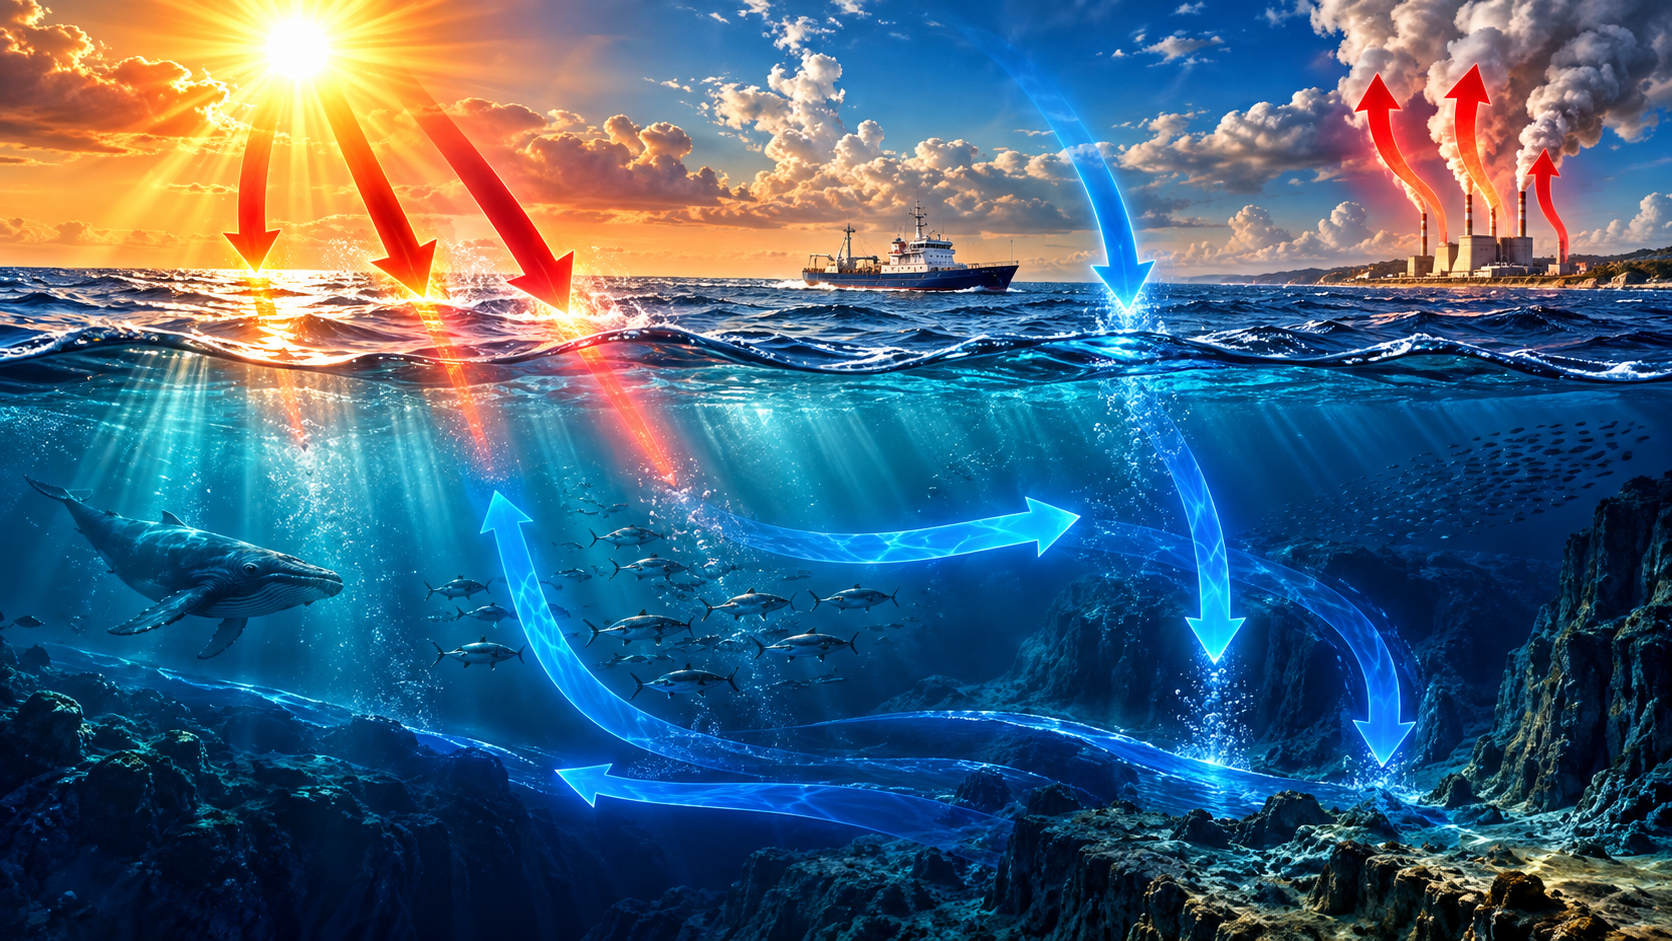
\includegraphics[width=\linewidth]{figures/ch04/ch04-04a-schematic-bad.png}
\end{minipage}\hfill
\begin{minipage}[c]{0.48\linewidth}\centering
\resizebox{\linewidth}{!}{\hbox{\setlength{\linewidth}{\textwidth}% FIG ch04-04b schematic labels (English)
\usetikzlibrary{positioning}
\begin{tikzpicture}
\node[anchor=south west,inner sep=0] (img) at (0,0) {%
  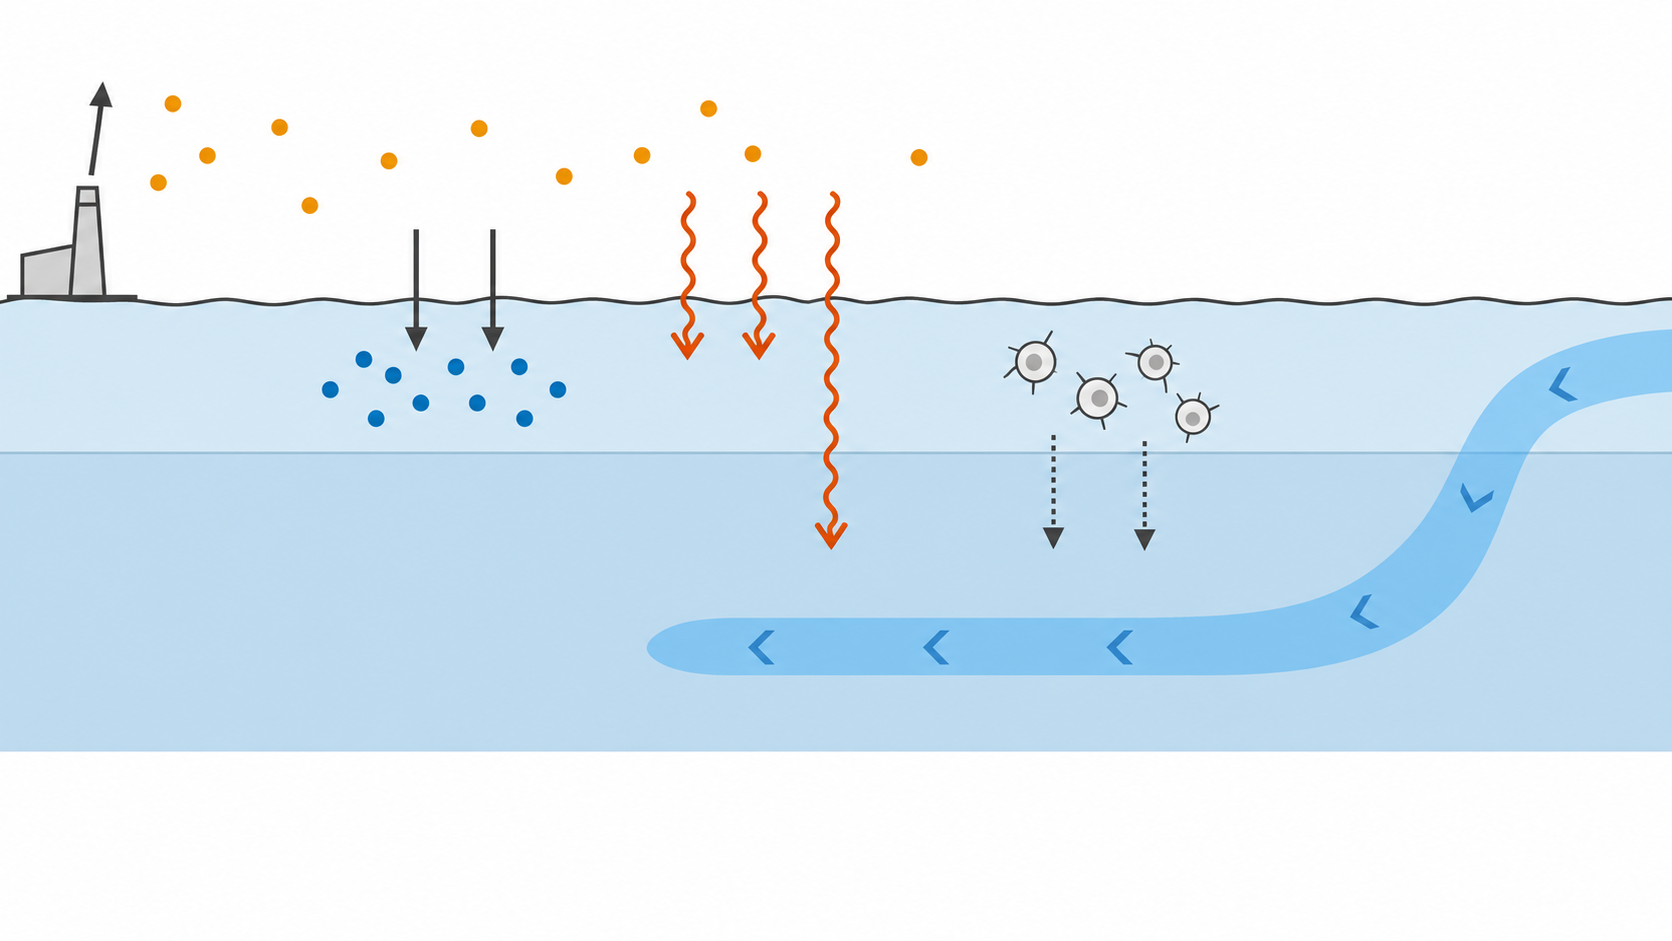
\includegraphics[width=\linewidth]{figures/ch04/ch04-04b-schematic-base.png}};
\begin{scope}[x={(img.south east)},y={(img.north west)},font=\sffamily\small]
  \node at (0.92,0.90) {Atmosphere};
  \node at (0.92,0.66) {Mixed layer};
  \node at (0.92,0.35) {Ocean interior};
  \node[align=left] at (0.06,0.93) {Anthropogenic emissions};
  \node at (0.30,0.88) {CO\textsubscript{2}};
  \node at (0.33,0.70) {Air--sea gas exchange};
  \node at (0.30,0.60) {Dissolved inorganic carbon};
  \node at (0.55,0.70) {Heat uptake};
  \node[align=center] at (0.80,0.45) {Sinking and transport\\of water};
  \node at (0.48,0.62) {Phytoplankton};
  \node[align=center] at (0.48,0.42) {Sinking particles\\(biological pump)};
  \node[align=center,font=\scriptsize] at (0.50,0.04) {%
    Legend: carbon flux / heat flux / water transport / sinking particles};
\end{scope}
\end{tikzpicture}
}}
\end{minipage}
\caption{The schematic follows the same visual language as the data figures. Left (deliberately inconsistent): glossy 3D rendering, a decorative sun and ship, unrequested whales and fish added by the model, and single-colour arrows standing for multiple processes. Right: redrawn to the specification using a text-free base image with TikZ overlay labels; semantic colour is reserved for atmospheric $\text{CO}_2$ (orange), seawater dissolved inorganic carbon (blue), heat (vermilion), and water transport (sky blue), with a distinct arrow shape for each process. Both are model-generated schematics, not to scale.}\label{fig:ch04-04}
\end{figure}

Notice also how the right panel of Figure~\ref{fig:ch04-04} respects the scientific boundary of the \textbf{biological pump}. Phytoplankton fix carbon and export sinking particulate organic carbon to the deep ocean (dotted arrows), but this biological pump mainly cycles \textit{natural} carbon; net oceanic uptake of \textbf{anthropogenic $\text{CO}_2$} since industrialization is governed primarily by air--sea gas exchange, carbonate buffer chemistry, and physical circulation (Sabine et al., 2004; Gruber et al., 2019; Fox-Kemper et al., 2023; Canadell et al., 2023). The right panel therefore places the main anthropogenic uptake pathway (left-middle straight dark-gray arrows $\rightarrow$ blue DIC dots $\rightarrow$ right-hand sky-blue sinking water band) separately from the phytoplankton cells and thinner dotted export arrows in the middle-right, avoiding the visual misconception that phytoplankton directly pump anthropogenic $\text{CO}_2$ into the deep ocean.

\section{Constrain with Prompts, Then Check Every Item}

Enforcing a visual specification with AI tools requires recognizing two practical realities. First, \textbf{conversational AI assistants do not know subfield conventions and may recommend retracted papers when asked to justify a figure design}---for instance, a high-profile 2018 \textit{Nature} paper estimating ocean heat uptake from atmospheric $\text{O}_2$ and $\text{CO}_2$ (Resplandy et al., 2018) was retracted in 2019 over uncertainty and trend-method errors. Every reference must be checked for retraction status via Crossref. Second, \textbf{\scidraw{} currently has no project-level or cross-session style memory}, and interface style presets are no substitute for your manuscript specification.

The reliable workflow is to save your one-page specification as a versioned document (Figure~\ref{fig:ch04-02}), distil it into two copy-ready \textbf{style blocks}, paste the relevant block at the start of every new session, and verify each rendered figure item by item. The core clauses of our specification (v1) are summarized below:

\begin{BookNote}
\textbf{Core Clauses of the One-Page Visual Specification (v1):}
\begin{itemize}
\item \textbf{A.\ Semantic colours (Okabe--Ito base):} Atmospheric carbon \texttt{\#E69F00} (orange: Fig.\ 2a, Fig.\ 4a atmospheric growth, Fig.\ 1 atmospheric $\text{CO}_2$ dots; never for heat or ocean variables); ocean carbon \texttt{\#0072B2} (blue: Fig.\ 2b seawater $p\text{CO}_2$, Fig.\ 4 ocean sink and share, Fig.\ 1 DIC dots; never for water background or heat); land carbon \texttt{\#009E73} (bluish green: Fig.\ 4a land sink only; never for phytoplankton icons); heat \texttt{\#D55E00} (vermilion: Fig.\ 3 depth curves and Fig.\ 1 heat arrows; never for carbon); seawater pH \texttt{\#CC79A7} (reddish purple: Fig.\ 2c only); anthropogenic emissions \texttt{\#3C3C3C} (dark gray); water transport \texttt{\#56B4E9} (sky blue: Fig.\ 1 circulation band only); neutral grays \texttt{\#F2F2F2}, \texttt{\#BDBDBD}, \texttt{\#7A7A7A} (backgrounds, icon fills, reference lines).
\item \textbf{B.\ Type hierarchy at final size:} Width $174\ \text{mm}$ (double column) for Figs.\ 1, 2, 4; $85\ \text{mm}$ (single column) for Fig.\ 3. Panel letters $8\ \text{pt}$ bold lowercase \textbf{a}, \textbf{b}, \textbf{c} (top-left outside axes); axis labels $7\ \text{pt}$ regular; ticks and direct curve labels $6\ \text{pt}$ regular (direct labels match series colour); schematic overlay labels $7\ \text{pt}$ (objects) and $6\ \text{pt}$ (processes). No internal figure titles; parenthetical SI units ($10^{22}\ \text{J}$, $\text{GtC yr}^{-1}$, $\mu\text{atm}$, ppm).
\item \textbf{C--E.\ Lines, arrows, and icons:} Follow Tables~\ref{tab:ch04-lines} and \ref{tab:ch04-arrows}. Icons use $0.75\ \text{pt}$ \texttt{\#3C3C3C} rounded outlines and neutral gray fills, with no gradients, shadows, or 3D effects; exclude sun, ships, icebergs, whales, and fish.
\item \textbf{F.\ Layout and export:} Keep only left and bottom axes ($0.6\ \text{pt}$, outward ticks), no grids, direct labels instead of legend boxes, $4\ \text{mm}$ panel gap; export vector PDF and high-resolution PNG with identical geometry across language editions.
\end{itemize}
\end{BookNote}

At the start of each new data-plotting session in \scidraw{} Scientific Visualization (\sdtool{sci-vis}), paste this data-figure style block:

\begin{Prompt}
Apply this paper-wide figure style exactly (visual spec v1):
- Colours by meaning, no other hues: atmospheric CO2 #E69F00; ocean carbon
  #0072B2; land carbon #009E73; heat #D55E00; seawater pH #CC79A7;
  emissions #3C3C3C; neutral grays #7A7A7A and #BDBDBD only.
- Monthly values: 0.5 pt line in a 50% lighter tint of the series colour.
  Deseasonalized or smoothed values: 1.2 pt solid line. Discrete cruise samples:
  small dots, no connecting line. Uncertainty: band in the series colour at 20%
  opacity, no edge line. Reference lines: 0.5 pt dashed #7A7A7A.
- Sans-serif font. Axis labels 7 pt, tick labels 6 pt, panel letters 8 pt bold
  lowercase (a, b, c) outside the top-left of each axes.
- No title inside the figure, no grid, no legend box: label each series
  directly at its right end in the series colour.
- Only left and bottom axes, 0.6 pt, ticks pointing outward.
- Final size 174 mm wide x 60 mm high.
Keep every data value unchanged: do not smooth, resample, interpolate or drop
rows unless I ask.
\end{Prompt}

When generating a schematic in AI Drawing (\sdtool{ai-drawing}) or via the Mechanism Figure Generator (\sdtool{mechanism-figure-generator}), paste the schematic style block:

\begin{Prompt}
Flat 2D scientific schematic of ocean heat and carbon uptake, landscape 16:9,
pure white background. ABSOLUTELY NO TEXT: no letters, no words, no numbers, no
symbols, no labels, no legend, no title.
STYLE (paper-wide visual spec v1): flat vector illustration; all outlines 0.75 pt
dark gray #3C3C3C with rounded joins; no gradients, no shadows, no highlights,
no 3D, no glow, no texture, no realistic water. Icons use neutral fills only
(#F2F2F2, #BDBDBD). Colour is used ONLY for the following quantities:
orange #E69F00 = CO2 in the atmosphere; blue #0072B2 = dissolved inorganic
carbon in seawater; vermilion #D55E00 = heat; sky blue #56B4E9 = water
transport. Nothing else may use these colours.
REGIONS (top to bottom): Top 25% atmosphere, white; thin dark gray gently wavy
line at 25% height (sea surface); 25-45% surface mixed layer (#DCEBF5); 45-90%
ocean interior (#C9DEEE); bottom 10% empty white reserved for a legend.
DO NOT DRAW: sun, rays, clouds, ships, fish, ice, land masses other than the
short ground line, sea floor details, coral, bubbles, any charts or data.
\end{Prompt}

Keep two precautions in mind when using \sdtool{sci-vis}. First, upload integrity checks (verifying file hashes, byte counts, and row counts) confirm only that the input file was not truncated, not that units, pH scales, anomaly baselines, or colours are scientifically valid. Second, multi-turn conversational edits often trigger \textbf{style drift}: asking to ``add a thin vertical dashed line at December 2022'' can cause regenerated code to quietly revert tick font sizes to library defaults or reintroduce a legend box. Re-verify colours, font sizes, and line styles after every edit, use version history to roll back when drift occurs, and run the Figure Checker (\sdtool{figure-checker}) to screen resolution, grayscale contrast, and colour-vision risk before final export.

\section{Case Study: Turning Four Standalone Figures into One Cohesive Set}

We now follow Maya's four figures from data inventory and specification drafting through redrawing and cross-figure verification.

\textbf{Step 1: Inventory the raw datasets and quality-control rules.} Four public datasets were downloaded on 29 October 2026 (Table~\ref{tab:ch04-sources}). In Figure 2, Mauna Loa atmospheric $\text{CO}_2$ is a \textbf{dry-air mole fraction} ($\text{ppm}$), whereas Station ALOHA surface seawater $p\text{CO}_2$ is an \textbf{in situ partial pressure} ($\mu\text{atm}$) calculated from DIC and total alkalinity. Because the two quantities have different physical dimensions despite sharing numerical values near $300\text{--}430$, they are plotted in separate side-by-side panels (\textbf{a}, \textbf{b}, \textbf{c}) rather than on a single axis.

\begin{table}[htbp]\centering\scriptsize
\setlength{\tabcolsep}{2.5pt}
\renewcommand{\arraystretch}{1.12}
\caption{Public datasets, quality-control rules, and attribution requirements for the four case-study figures (downloaded 29 October 2026).}\label{tab:ch04-sources}
\begin{tabularx}{\linewidth}{@{}>{\raggedright\arraybackslash}p{20mm}>{\raggedright\arraybackslash}p{24mm}>{\raggedright\arraybackslash}p{18mm}Y>{\raggedright\arraybackslash}p{26mm}@{}}
\toprule
\textbf{Dataset (Figure)} & \textbf{File and size} & \textbf{Fields and units} & \textbf{Data processing and QC assertions} & \textbf{Licence and attribution} \\
\midrule
Mauna Loa atmospheric $\text{CO}_2$ (Fig.\ 2a) & \path{co2_mm_mlo.csv}; 823 rows (1958-03 to 2026-09) & \texttt{average}, \path{deseasonalized} ($\text{ppm}$) & Skip \texttt{\#} header lines; assert zero $-99.99$ missing values (mean $361.44\ \text{ppm}$); apply no extra smoothing; mark the Dec 2022--Jul 2023 Mauna Loa eruption relocation to Maunakea & U.S.\ federal government public data; credit both NOAA GML and Scripps (Keeling) \\
HOT Station ALOHA carbonate system (Fig.\ 2b, c) & \path{HOT_surface_CO2.txt}; 355 rows (from 1988-10-31) & \path{pCO2calc_insitu} ($\mu\text{atm}$), \path{pHcalc_insitu} & Skip 8-line header; replace values $\le -900$ (missing code $-999$) with \texttt{NaN}, leaving 346 valid cruises; parse two-digit years into 1988--2026; verify pH scale in \path{HOT_surface_CO2_readme.pdf} for caption & Cite Dore et al.\ (2009) per file header; no explicit open licence stated, so redrawing requires strict citation \\
Global ocean heat content anomaly (Fig.\ 3) & \path{pent_h22-w0-700m.dat} and \texttt{2000m.dat}; 67 rows each & \texttt{YEAR} (1957.5--2023.5), \texttt{WO}, \texttt{WOse} ($10^{22}\ \text{J}$) & Assert identical midpoint years and row counts across both depth files (means $3.84$ and $5.09\times 10^{22}\ \text{J}$); shade $\text{WO} \pm 1\ \text{WOse}$; confirm climatological baseline period in NCEI documentation & NOAA NCEI U.S.\ government work; cite Levitus et al.\ (2012) \\
Global Carbon Budget 2025 (Fig.\ 4) & \path{GlobalCarbonBudget_v2025.xlsx}; 66 rows (1959--2024) & Emissions and three sinks ($\text{GtC yr}^{-1}$) & Read sheet \texttt{Global Carbon Budget} (header row 22); total emissions = fossil + land-use change; shade mean uncertainties ($\pm 0.4$ ocean, $\pm 0.5$ land); compute ocean share (mean $27.01\%$) and 10-yr centred running mean in panel b & Fair Use Statement; cite Friedlingstein et al.\ (2026) and acknowledge Global Carbon Project \\
\bottomrule
\end{tabularx}
\end{table}

\textbf{Step 2: Redraw the conceptual schematic (Fig.\ 1) and audit generative deviations.} Compare the prompt used for the inconsistent 3D schematic on the left of Figure~\ref{fig:ch04-04}:

\begin{Prompt}
A glossy, highly polished 3D illustration of an ocean cross-section for a
climate science paper, landscape 16:9. Photorealistic blue waves on top, a
bright sun with radiating rays in a gradient orange-to-blue sky, a small ship
on the surface, shiny glass-like water with caustics and depth of field.
Thick glowing red 3D arrows go from the sky into the water and also from a
factory into the sky; thick glowing blue 3D arrows curve through the water and
also go from the air into the water. Dramatic lighting, lens flare, strong
shadows, saturated colors. No text, no letters, no numbers, no labels.
\end{Prompt}

Requesting ``glossy 3D'', ``photorealistic blue waves'', and ``dramatic lighting'' while assigning red and blue arrows to multiple processes directly caused the visual conflicts in Table~\ref{tab:ch04-diag}---and without an exclusion list, the model added a whale, fish schools, and reefs.

To redraw the right panel of Figure~\ref{fig:ch04-04}, we appended the following seven object and process instructions to the schematic style block from Section 4.5 (full prompt in the \texttt{cases/} directory of the book repository):

\begin{Prompt}
OBJECTS AND PROCESSES (draw exactly these, nothing else):
1. Top-left: one simple factory chimney icon in neutral gray on a short ground
   line, with one straight dark gray arrow (filled head) rising into the air.
2. Atmosphere: about 12 small orange dots scattered in the left and middle.
3. Air-sea gas exchange: two straight dark gray arrows with filled heads, going
   down from the atmosphere through the sea surface into the mixed layer.
4. Mixed layer: about 10 small blue #0072B2 dots near the two arrows.
5. Heat uptake: three vermilion wavy arrows with open V-shaped heads, going down
   into the mixed layer; the rightmost continues into the ocean interior.
6. Water transport: on the right, one broad semi-transparent sky-blue band from
   the mixed layer curving down into the interior and running leftward, with
   chevron marks pointing along the flow.
7. Biological pump: 3-4 small round phytoplankton cell icons (neutral fill, gray
   outline) in the mixed layer, and two dotted dark gray arrows pointing down.
Leave white space around each process for labels.
\end{Prompt}

Generating three candidates from this prompt and auditing each image reveals how generative outputs behave in practice:
\begin{itemize}
\item \textbf{Candidate 1 (rejected for contradictory flow direction):} All major objects appeared, but inside the sky-blue transport band on the right, upper and middle chevrons pointed up-right while bottom chevrons pointed left, making the flow collide head-on with itself.
\item \textbf{Candidate 2 (selected for Figure~\ref{fig:ch04-04}, right):} All seven object groups and four arrow types were present, chevrons inside the transport band pointed consistently down-left and leftward along the flow, and no text or forbidden decorative objects appeared.
\item \textbf{Candidate 3 (rejected):} Flow direction was consistent, but the model added unrequested spine-like protrusions to the phytoplankton cells, thickened the dotted arrows, and yielded a slightly lower luminance contrast for the vermilion heat arrows against the interior background under simulated deuteranomaly ($2.17:1$ vs.\ $2.36:1$ in Candidate 2).
\end{itemize}

A pixel audit of the selected Candidate 2 base image still uncovers three real deviations: (1) \textbf{approximate hex colours}---median RGB values across object regions measured \texttt{\#ED9106} for atmospheric orange dots (spec \texttt{\#E69F00}), \texttt{\#0571BA} for seawater blue dots (spec \texttt{\#0072B2}), \texttt{\#DD4E0A} for vermilion heat arrows (spec \texttt{\#D55E00}), and \texttt{\#3F3F40} for dark-gray carbon arrows (spec \texttt{\#3C3C3C}), with zero pixels matching the exact target hex strings and slight shading across the water layers and smokestack; (2) \textbf{shifted layer proportions and object placement}---the sea surface, mixed-layer base, and bottom legend margin fell at roughly $32\%$, $48\%$, and $80\%$ of height rather than $25\%$, $45\%$, and $90\%$, and the four phytoplankton cells sat in the middle-right of the mixed layer, so the overlaid ``Phytoplankton'' label placed at the preset centre coordinate landed in open water to their left (Figure~\ref{fig:ch04-04}, right) and requires a rightward nudge in TikZ; and (3) \textbf{native resolution limits}---at $174\ \text{mm}$ width, the $1672 \times 941\ \text{px}$ raster image provides $244\ \text{ppi}$ with no editable vector stroke weights.

\textbf{Step 3: Redraw the three data figures (Figs.\ 2--4) to the specification.} Importing all style constants from a shared module produced Figures~\ref{fig:ch04-05}--\ref{fig:ch04-07} (Table~\ref{tab:ch04-revisions}).

\begin{figure}[htbp]\centering
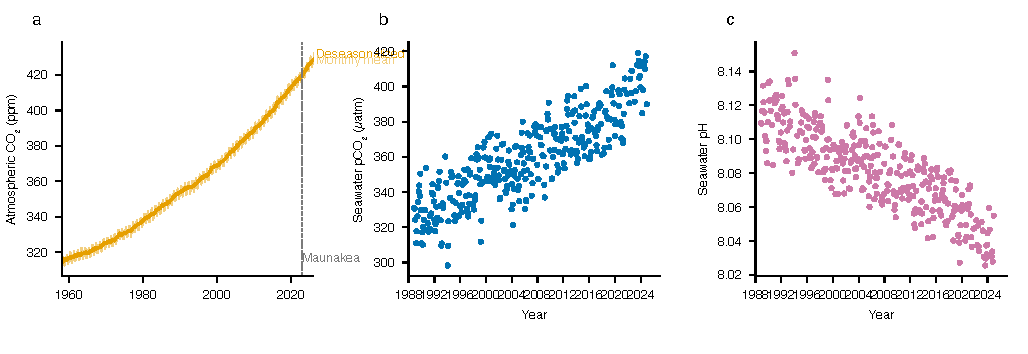
\includegraphics[width=\linewidth]{figures/ch04/ch04-05-fig2-carbonate-en.pdf}
\caption{Paper Fig.\ 2 redrawn to the specification: atmospheric $\text{CO}_2$ and the surface seawater carbonate system in the subtropical North Pacific. (a) Monthly mean (thin light-orange line) and deseasonalized (thick orange line) atmospheric $\text{CO}_2$ at Mauna Loa Observatory; March 1958--April 1974 data are from Scripps, and December 2022--July 2023 observations were made at Maunakea after the Mauna Loa eruption (gray dashed line). (b) Surface seawater $p\text{CO}_2$ at Station ALOHA (HOT), calculated in situ from DIC and total alkalinity; one dot per cruise. (c) Surface seawater pH at the same station (calculated at in situ temperature; pH scale to be confirmed). Data: NOAA GML and Scripps; HOT (Dore et al., 2009), downloaded 29 October 2026.}\label{fig:ch04-05}
\end{figure}

In Figure~\ref{fig:ch04-05} (Paper Fig.\ 2), panel \textbf{a} plots Mauna Loa $\text{CO}_2$ in semantic orange (\texttt{\#E69F00}) with the Maunakea relocation dashed line; panel \textbf{b} plots 346 valid cruises of surface seawater $p\text{CO}_2$ as unlinked ocean-carbon blue dots (\texttt{\#0072B2}); and panel \textbf{c} plots surface pH in reddish purple (\texttt{\#CC79A7}). Checking at $100\%$ print size catches three remaining layout details: at the top right of panel \textbf{a}, ``Deseasonalized'' and ``Monthly mean'' overlap vertically and collide with the ``420'' y-tick label of panel \textbf{b}; in panels \textbf{b} and \textbf{c}, the 4-year x-tick labels crowd together and should be widened to 10-year intervals; and the dropped subscript ``2'' in the y-axis labels of panels \textbf{a} and \textbf{b} needs explicit math-mode subscripting.

\begin{figure}[htbp]\centering
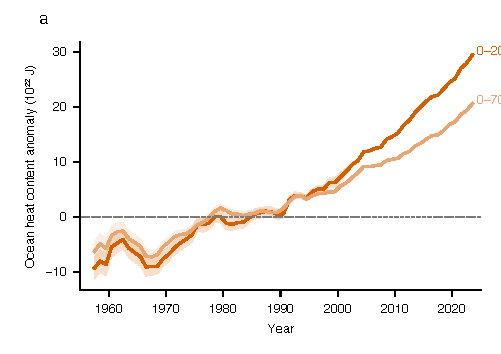
\includegraphics[width=0.58\linewidth]{figures/ch04/ch04-06-fig3-ohc-en.pdf}
\caption{Paper Fig.\ 3 redrawn to the specification: global ocean heat content anomaly. Pentadal heat content anomalies for $0\text{--}700\ \text{m}$ (light vermilion) and $0\text{--}2000\ \text{m}$ (dark vermilion), in $10^{22}\ \text{J}$, plotted at five-year window midpoints; shading shows $\pm 1$ standard error from NCEI, and the dashed line marks zero. The climatological baseline period must be confirmed in NCEI documentation. Data: NOAA NCEI (method of Levitus et al., 2012, and updates).}\label{fig:ch04-06}
\end{figure}

In Figure~\ref{fig:ch04-06} (Paper Fig.\ 3, single-column width $85\ \text{mm}$), both curves use the vermilion heat hue (\texttt{\#D55E00}) separated by lightness, with $\pm 1\ \text{WOse}$ bands and a dashed zero line showing sustained ocean heat uptake (von Schuckmann et al., 2023). Inspecting the right edge shows that ``$0\text{--}2000\ \text{m}$'' and ``$0\text{--}700\ \text{m}$'' are clipped to ``\texttt{0--20}'' and ``\texttt{0--70}'', demonstrating that direct right-end labels require widening the right margin or upper x-axis limit.

\begin{figure}[htbp]\centering
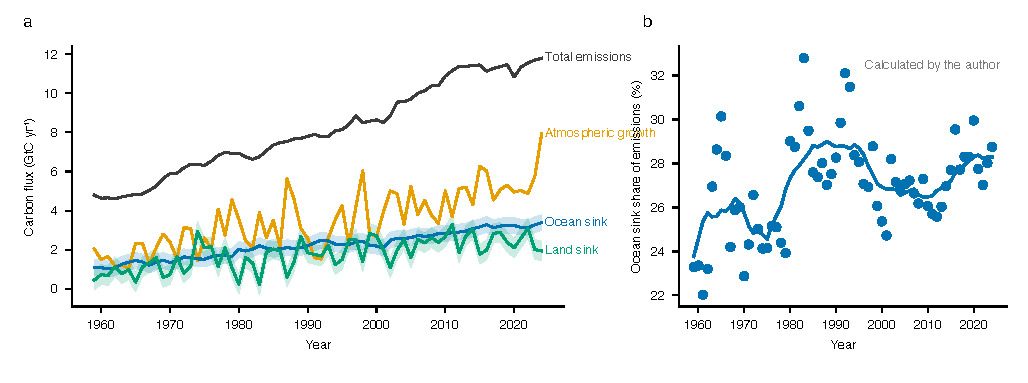
\includegraphics[width=\linewidth]{figures/ch04/ch04-07-fig4-budget-en.pdf}
\caption{Paper Fig.\ 4 redrawn to the specification: partitioning of anthropogenic $\text{CO}_2$ emissions. (a) Combined fossil and land-use change emissions (dark gray) with atmospheric growth (orange), ocean sink (blue), and land sink (bluish green), in $\text{GtC yr}^{-1}$; bands show mean GCB uncertainties ($\pm 0.4$ ocean, $\pm 0.5\ \text{GtC yr}^{-1}$ land). (b) Ocean sink share of total emissions, calculated by the author from GCB 2025 data (dots, annual values; curve, 10-year centred running mean). Budget imbalance and cement carbonation sink are omitted. Data: Global Carbon Budget 2025 (Friedlingstein et al., 2026).}\label{fig:ch04-07}
\end{figure}

In Figure~\ref{fig:ch04-07} (Paper Fig.\ 4), panel \textbf{a} replaces the rainbow stacked area plot with four semantic curves and uncertainty bands, while panel \textbf{b} plots the author-computed ocean sink share (mean $27.01\%$) as blue annual dots and a 10-year running mean marked ``Calculated by the author''. At $100\%$ zoom, ``Atmospheric growth'' slightly grazes the left spine of panel \textbf{b}, and the y-axis unit requires an explicit minus sign ($\text{GtC yr}^{-1}$).

\begin{table}[htbp]\centering\footnotesize
\setlength{\tabcolsep}{3pt}
\renewcommand{\arraystretch}{1.15}
\caption{Revision log from the inconsistent draft (Figure~\ref{fig:ch04-01}) to the redrawn figures (Figures~\ref{fig:ch04-04}--\ref{fig:ch04-07}).}\label{tab:ch04-revisions}
\begin{tabularx}{\linewidth}{@{}>{\raggedright\arraybackslash}p{14mm}Y>{\raggedright\arraybackslash}p{20mm}>{\raggedright\arraybackslash}p{36mm}@{}}
\toprule
\textbf{Figure} & \textbf{Specific revisions applied} & \textbf{Clause} & \textbf{Verification and audit notes} \\
\midrule
Fig.\ 1 & Removed 3D gloss, sun, ship, whale, and fish; generated flat 2D base; redrew four process arrows per Table~\ref{tab:ch04-arrows}; added TikZ labels & Clauses A, D, E & Rejected Candidate 1 (flow collision), chose Candidate 2; noted approximate hex values and rightward phytoplankton offset \\
Fig.\ 2a & Changed dual red lines to orange \texttt{\#E69F00} ($0.5\ \text{pt}$ light monthly + $1.2\ \text{pt}$ deseasonalized); added Maunakea dashed line & Clauses A, C & Eyedropper hex check; caught end-label overlap and collision with panel b y-ticks \\
Fig.\ 2b, c & Changed connected green/blue lines to unlinked $2.5\ \text{pt}$ dots in \texttt{\#0072B2} (ocean carbon) and \texttt{\#CC79A7} (pH) & Clauses A, C & Verified 346 valid cruises unlinked; noted crowded 4-yr x-ticks to widen to 10-yr spacing \\
Fig.\ 3 & Replaced red/green lines with two lightnesses of vermilion (\texttt{\#D55E00}); added $\pm 1\ \text{WOse}$ bands and zero line; fixed \texttt{1e23} offset & Clauses A, B, C & Separable under deuteranomaly simulation (Figure~\ref{fig:ch04-03}); right-end labels clipped, need wider right margin \\
Fig.\ 4 & Replaced \texttt{jet} stacked areas with four semantic curves + bands; added panel b ocean share marked ``Calculated by the author'' & Clauses A, B, C & Verified 66-yr values against workbook; ``Atmospheric growth'' label grazes panel b spine \\
All four & Unified sans-serif font and 8/7/6 pt hierarchy; bold lowercase \textbf{a}--\textbf{c}; removed internal titles, grids, and legend boxes & Clauses B, F & Measured point sizes in $100\%$ PDF; caught silent dropout of Unicode subscript 2 and superscript minus \\
\bottomrule
\end{tabularx}
\end{table}

\textbf{Step 4: Side-by-side contact-sheet comparison, finalized captions, and verification log.} Assembling the four revised figures into the same $2 \times 2$ layout as Figure~\ref{fig:ch04-01} with a bottom semantic colour bar yields Figure~\ref{fig:ch04-08}.

\begin{figure}[htbp]\centering
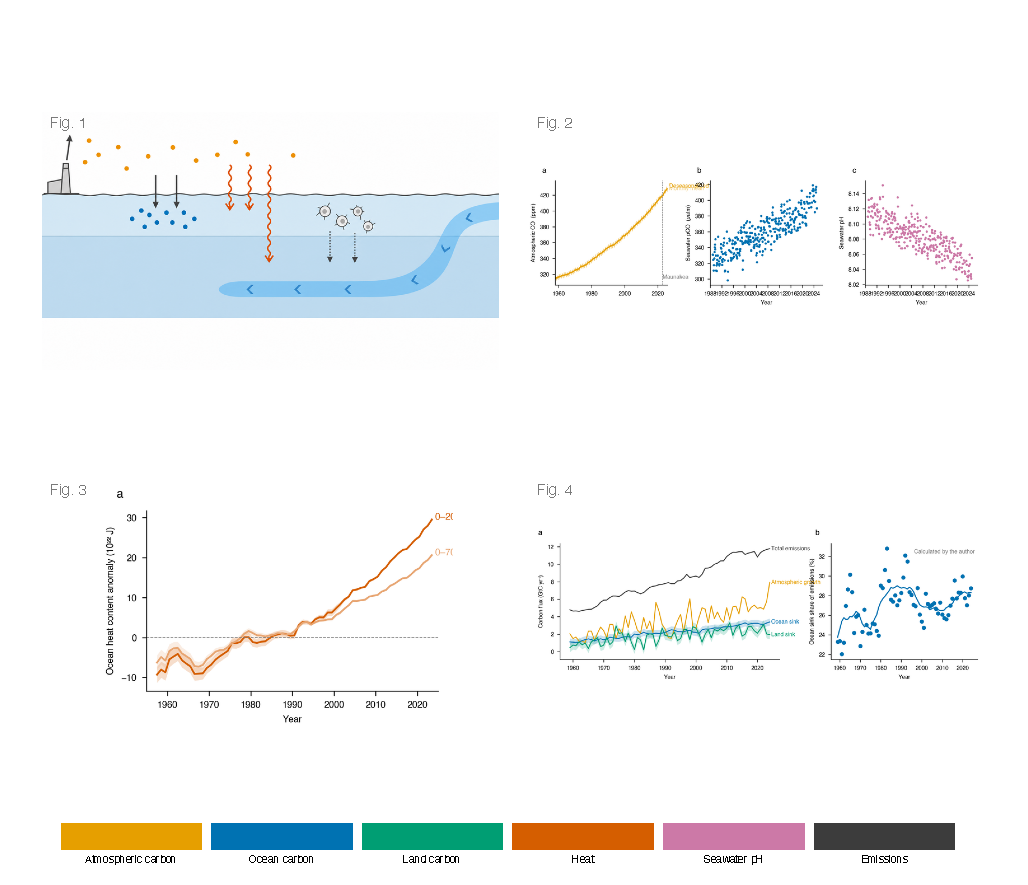
\includegraphics[width=\linewidth]{figures/ch04/ch04-08-consistent-set-en.pdf}
\caption{The four manuscript figures after applying the one-page visual specification. Every semantic colour carries a single meaning across the paper (bottom strip), and fonts, sizes, panel letters, line styles, and arrow shapes are unified. Compared with Figure~\ref{fig:ch04-01}, the underlying data are identical; only the visual language has changed.}\label{fig:ch04-08}
\end{figure}

Comparing Figure~\ref{fig:ch04-08} with Figure~\ref{fig:ch04-01}, readers can trace orange (atmospheric carbon) directly across Fig.\ 1, Fig.\ 2a, and Fig.\ 4a; trace blue (ocean carbon) across Fig.\ 1, Fig.\ 2b, and Fig.\ 4a, b; and trace vermilion (heat) from Fig.\ 1 to Fig.\ 3 without consulting a legend box. The finalized caption for Paper Fig.\ 1 is given below, followed by the cross-figure verification log (Table~\ref{tab:ch04-verify}).

\begin{BookNote}
\textbf{Finalized Caption for Paper Figure 1:} \textbf{Figure 1 | Main pathways of ocean heat and anthropogenic $\text{CO}_2$ uptake.} Excess heat enters the surface mixed layer across the air--sea interface (wavy arrows) and is carried into the ocean interior by mixing and the sinking of water masses (pale-blue band). Anthropogenic $\text{CO}_2$ dissolves into surface seawater by air--sea gas exchange (straight arrows), raising seawater $p\text{CO}_2$ and lowering pH, and is likewise transported into the interior. Phytoplankton fix carbon that is exported as sinking particles (dotted arrows); this biological pump mainly moves carbon of the natural cycle, whereas uptake of anthropogenic $\text{CO}_2$ is governed chiefly by gas exchange, seawater chemistry, and circulation. Schematic, not to scale; regional and seasonal variations, sea ice, sediments, and river inputs are omitted. Compiled from Sabine et al.\ (2004), Gruber et al.\ (2019), and IPCC AR6 WGI Chapters 5 and 9 (Canadell et al., 2023; Fox-Kemper et al., 2023).
\end{BookNote}

\begin{table}[htbp]\centering\footnotesize
\setlength{\tabcolsep}{3pt}
\renewcommand{\arraystretch}{1.15}
\caption{Cross-figure verification log for the four case-study manuscript figures.}\label{tab:ch04-verify}
\begin{tabularx}{\linewidth}{@{}>{\raggedright\arraybackslash}p{38mm}YYYY@{}}
\toprule
\textbf{Verification item} & \textbf{Fig.\ 1} & \textbf{Fig.\ 2} & \textbf{Fig.\ 3} & \textbf{Fig.\ 4} \\
\midrule
Semantic colours match Clause A across figures & Pass (hex approximate) & Pass & Pass & Pass \\
Separable under CVD simulation and in grayscale & Separable via arrow shapes & Separate panels, no conflict & Pass (Figure~\ref{fig:ch04-03}) & Pass (with direct labels) \\
Type sizes match 8/7/6 pt at $100\%$ print size & Pass & Pass & Pass & Pass \\
Panel letters and units consistent, no glyph dropout or clipping & Nudge ``Phytoplankton'' label right & Fix subscript 2, label overlap, 4-yr ticks & Widen right margin for clipped labels & Fix minus sign in $\text{yr}^{-1}$ and label margin \\
Lines and arrows match Tables~\ref{tab:ch04-lines} and \ref{tab:ch04-arrows} & Pass & Pass & Pass & Pass \\
Years and row counts match raw files & Not applicable & 823 rows / 346 cruises & 67 rows (both depths) & 66 rows (1959--2024) \\
Author calculations and uncertainties in caption & Not applicable & Confirm pH scale in readme & Confirm baseline in NCEI docs & Marked ``Calculated by the author'' \\
Citations complete and domain review scheduled & Pending oceanographer review & NOAA GML, Scripps, HOT cited & NOAA NCEI, Levitus cited & GCB 2025, GCP cited \\
\bottomrule
\end{tabularx}
\end{table}

\section{What AI Can and Cannot Do in This Step}

Table~\ref{tab:ch04-01} summarizes the division of responsibilities between AI tools and the author when establishing a paper-wide visual language.

\begin{table}[htbp]\centering\scriptsize
\setlength{\tabcolsep}{3pt}
\renewcommand{\arraystretch}{1.12}
\caption{What AI can do, what it cannot reliably do, and what the author must verify when building a paper-wide visual language.}\label{tab:ch04-01}
\begin{tabularx}{\linewidth}{@{}>{\raggedright\arraybackslash}p{19mm}YYY@{}}
\toprule
\textbf{Step} & \textbf{What AI can do} & \textbf{What AI cannot do / where it fails} & \textbf{What the author must verify} \\
\midrule
Drafting the specification & Conversational AI can propose an initial semantic colour table and type hierarchy from your figure list and suggest accessible palettes & Does not know your subfield's colour conventions or journal dimensions; may cite non-existent or retracted papers as justification & Check every clause against domain norms and journal guidelines; verify all DOIs and retraction statuses via Crossref \\
Cross-figure memory & --- & \scidraw{} has no project-level style memory and does not remember your specification across sessions or tools & Save the specification as a versioned document; paste the style block into every new session \\
Applying style to data plots & \sdtool{sci-vis} generates plots from a style block, applies conversational edits, and restores earlier versions & Multi-turn edits can trigger style drift (reverting font sizes, restoring legends, or clipping labels); ``done'' does not mean compliant & Sample hex values, measure type at $100\%$ size, check line styles after each turn, and save compliant versions \\
Data integrity checks & \sdtool{sci-vis} checks SHA-256 hashes, byte counts, and row counts of uploaded files & Proves only that no rows were dropped on upload, not that units, pH scales, baselines, or calculations are right & Check start/end dates, row counts, units, and baselines against raw files and documentation \\
Applying style to schematics & Drawing and reference-image editing generate flat schematics with approximate semantic colours & Hex colours, layer ratios, and stroke widths are approximate; may produce conflicting flow chevrons or extra objects & Compare multiple candidates, sample pixel colours, check arrow directions, remove extra objects, and align TikZ labels \\
CVD and technical checks & \sdtool{figure-checker} screens format, resolution, grayscale contrast, and algorithmic CVD risk & Does not audit science; numerical CVD simulation is an approximation and cannot replace human readers & Combine simulation and grayscale checks with review by a reader with CVD; verify science separately \\
Figure captions & \sdtool{figure-legend} drafts caption structure from a rendered figure & Does not know data provenance, processing, or baselines; must never invent them & Supply data sources, download dates, units, uncertainties, and author-calculated items yourself \\
\bottomrule
\end{tabularx}
\end{table}

\section{Chapter Checklist}

\begin{itemize}
\item I have a written one-page visual specification with a version number.
\item Every semantic colour encodes one quantity or reservoir, and every recurring quantity uses the same semantic colour across all figures.
\item Semantic colours do not exceed 6--7 hues; axes, reference lines, backgrounds, and icon bodies use neutral grays.
\item Colours sharing a panel remain distinguishable under colour-vision simulation and in grayscale, or have redundant shape, line-style, or direct-label encoding.
\item Continuous variables use perceptually uniform sequential or diverging colormaps, never rainbow colormaps.
\item Font sizes have been measured at $100\%$ final print size across all four levels (panel letters, axis labels, ticks, annotations).
\item One sans-serif typeface is used throughout, bilingual editions share identical geometry, and subscripts and superscripts have been checked at $200\%$ zoom for missing-glyph boxes or dropped characters.
\item Unit notation and panel letters (\textbf{a}, \textbf{b}, \textbf{c}) follow the same convention in every figure.
\item Every line style and schematic arrow shape has a single meaning, defined once in the legend.
\item Icons use neutral gray fills, match axis stroke weights, and omit unmentioned decorative objects.
\item The style block was pasted into every new session, and colours, font sizes, and margins were re-checked after every conversational edit.
\item Data sources, download dates, processing rules, and author-computed quantities are stated in the captions.
\item I have viewed all figures side by side on a single page at final print size.
\end{itemize}

\section{Exercises}

\begin{enumerate}
\item \textbf{(Pen and paper: Assign semantic colours to your paper)} List all quantities or categories across the figures of a paper you are writing (or a published paper in your field). (a) Group them into no more than six semantic roles; (b) assign each role an Okabe--Ito colour and state ``used for / never used for''; (c) find at least three violations in the existing figures and specify the fix; (d) explain whether your discipline has mandatory colour conventions (such as warm colours for temperature or blue-green for precipitation) and whether your table conflicts with them.
\item \textbf{(Colour-vision and grayscale check)} Pick one data figure from your paper. (a) Export a PNG and check colour-vision risk and grayscale contrast in the \scidraw{} Figure Checker (\sdtool{figure-checker}), or simulate three CVD types using \texttt{colorspacious}; (b) identify the hardest colour pair to distinguish under simulation; (c) resolve the conflict without adding a new hue by using lightness, line style, or direct labels; (d) explain why simulation cannot replace asking a human reader with CVD.
\item \textbf{(Hands-on with \scidraw{}: Constrain a dataset with a style block)} Download \texttt{co2\_mm\_mlo.csv} from NOAA GML, strip \texttt{\#} comment lines, and save a clean CSV (recording its SHA-256 hash and row count). (a) Upload it to \scidraw{} Scientific Visualization (\sdtool{sci-vis}), ask only ``Plot the atmospheric $\text{CO}_2$ time series'', and save the result; (b) open a new session, upload the same file, paste the data-figure style block from Section 4.5, and repeat the request; (c) add two follow-up edits (e.g., ``make the monthly mean line lighter'' and ``add a thin vertical line at December 2022''), checking after each turn whether colours or font sizes drifted; (d) compare versions (a), (b), and (c) in an audit table (colour, font size, line style, labels, row count) and write a one-sentence credit to NOAA GML and Scripps. \textit{(Note: The example figures in this chapter were generated by image models and companion scripts; prompts and generation records are available in the book repository.)}
\end{enumerate}

\section*{References}

{\sloppy
\begin{itemize}
\item Brewer CA. ColorBrewer 2.0: Color advice for cartography. \url{https://colorbrewer2.org}
\item Canadell JG, Monteiro PMS, Costa MH, Cotrim da Cunha L, Cox PM, Eliseev AV, Henson S, Ishii M, Jaccard S, Koven C, Lohila A, Patra PK, Piao S, Rogelj J, Syampungani S, Zaehle S, Zickfeld K. Global carbon and other biogeochemical cycles and feedbacks. In: \textit{Climate Change 2021: The Physical Science Basis. Contribution of Working Group I to the Sixth Assessment Report of the Intergovernmental Panel on Climate Change}. Cambridge University Press; 2023:673--816. doi:10.1017/9781009157896.007
\item Crameri F, Shephard GE, Heron PJ. The misuse of colour in science communication. \textit{Nature Communications}. 2020;11:5444. doi:10.1038/s41467-020-19160-7
\item Dore JE, Lukas R, Sadler DW, Church MJ, Karl DM. Physical and biogeochemical modulation of ocean acidification in the central North Pacific. \textit{Proceedings of the National Academy of Sciences}. 2009;106(30):12235--12240. doi:10.1073/pnas.0906044106
\item Fox-Kemper B, Hewitt HT, Xiao C, A\dh algeirsd\'ottir G, Drijfhout SS, Edwards TL, Golledge NR, Hemer M, Kopp RE, Krinner G, Mix A, Notz D, Nowicki S, Nurhati IS, Ruiz L, Sall\'ee J-B, Slangen ABA, Yu Y. Ocean, cryosphere and sea level change. In: \textit{Climate Change 2021: The Physical Science Basis. Contribution of Working Group I to the Sixth Assessment Report of the Intergovernmental Panel on Climate Change}. Cambridge University Press; 2023:1211--1362. doi:10.1017/9781009157896.011
\item Friedlingstein P, O'Sullivan M, Jones MW, et al. Global Carbon Budget 2025. \textit{Earth System Science Data}. 2026;18:3211--3288. doi:10.5194/essd-18-3211-2026
\item Gruber N, Clement D, Carter BR, Feely RA, van Heuven S, Hoppema M, Ishii M, Key RM, Kozyr A, Lauvset SK, Lo Monaco C, Mathis JT, Murata A, Olsen A, Perez FF, Sabine CL, Tanhua T, Wanninkhof R. The oceanic sink for anthropogenic $\text{CO}_2$ from 1994 to 2007. \textit{Science}. 2019;363(6432):1193--1199. doi:10.1126/science.aau5153
\item Krzywinski M. Elements of visual style. \textit{Nature Methods}. 2013;10(5):371. doi:10.1038/nmeth.2444
\item Levitus S, Antonov JI, Boyer TP, Baranova OK, Garcia HE, Locarnini RA, Mishonov AV, Reagan JR, Seidov D, Yarosh ES, Zweng MM. World ocean heat content and thermosteric sea level change (0--2000 m), 1955--2010. \textit{Geophysical Research Letters}. 2012;39:L10603. doi:10.1029/2012GL051106
\item NOAA Global Monitoring Laboratory. Trends in Atmospheric Carbon Dioxide (Mauna Loa, Hawaii) and Scripps Institution of Oceanography $\text{CO}_2$ Program. \url{https://gml.noaa.gov/ccgg/trends/} and \url{https://scrippsco2.ucsd.edu/}
\item Nu\~nez JR, Anderton CR, Renslow RS. Optimizing colormaps with consideration for color vision deficiency to enable accurate interpretation of scientific data. \textit{PLOS ONE}. 2018;13(8):e0199239. doi:10.1371/journal.pone.0199239
\item Okabe M, Ito K. Color Universal Design (CUD): How to make figures and presentations that are friendly to colorblind people. 2008. \url{https://jfly.uni-koeln.de/color/}
\item Rougier NP, Droettboom M, Bourne PE. Ten simple rules for better figures. \textit{PLoS Computational Biology}. 2014;10(9):e1003833. doi:10.1371/journal.pcbi.1003833
\item Sabine CL, Feely RA, Gruber N, Key RM, Lee K, Bullister JL, Wanninkhof R, Wong CS, Wallace DWR, Tilbrook B, Millero FJ, Peng T-H, Kozyr A, Ono T, Rios AF. The oceanic sink for anthropogenic $\text{CO}_2$. \textit{Science}. 2004;305(5682):367--371. doi:10.1126/science.1097403
\item von Schuckmann K, Mini\`ere A, Gues F, Cuesta-Valero FJ, Kirchengast G, Adusumilli S, Straneo F, et al. Heat stored in the Earth system 1960--2020: where does the energy go? \textit{Earth System Science Data}. 2023;15(4):1675--1709. doi:10.5194/essd-15-1675-2023
\item Wong B. Points of view: Color coding. \textit{Nature Methods}. 2010;7(8):573. doi:10.1038/nmeth0810-573
\item Wong B. Points of view: Typography. \textit{Nature Methods}. 2011;8(4):277. doi:10.1038/nmeth0411-277
\item Wong B. Points of view: Color blindness. \textit{Nature Methods}. 2011;8(6):441. doi:10.1038/nmeth.1618 (Author Correction: \textit{Nature Methods}. 2023;20:1442. doi:10.1038/s41592-023-01974-0)
\end{itemize}
\par}

\chapter{Visualizing Data with AI Assistance}

Lin Yue, a graduate student in ecology, had just compiled a morphometric dataset of adult breeding penguins from three species across the Palmer Archipelago in Antarctica. She needed a figure for her lab meeting and for the ``Study System'' subsection of her manuscript to compare body mass across the three species. Opening a conversational data-visualization tool, she uploaded the spreadsheet and typed: ``Make a professional bar chart comparing penguin body mass across species, formatted in journal style.'' Seconds later, a clean, colourful chart appeared: three solid bars representing the three species, each topped by a tiny black error bar.

At first glance, the chart looked ready for submission. At lab meeting, however, her advisor asked four basic questions that brought the presentation to a halt. First, did those short whiskers at the top of each bar represent one standard deviation (SD), one standard error of the mean (SEM), or a 95\% confidence interval (CI)? Second, how many measurement records stood behind each bar, and how had the tool handled the missing values scattered across the table? Third, penguin body mass exhibits pronounced sexual dimorphism—how much within-species sex difference was concealed by pooling females and males into a single bar? Fourth, why did the first two species, whose mean body masses differed by barely thirty grams, look almost two-fold different in an earlier draft where the software had automatically cropped the vertical axis?

In a scientific paper, a data figure is not page decoration; it is quantitative evidence that directly supports empirical claims. Conversational visualization tools save hours of looking up plotting syntax, yet whenever instructions are vague, the software silently makes a chain of unauthorized statistical and visual encoding decisions. Faced with any chart generated or modified with AI assistance, the first question is never ``Does this chart look polished?'' but ``Is this chart accurate, honest, and verifiable line by line against the raw data table?'' Starting from how to read a raw spreadsheet before touching plotting software, this chapter shows how to direct, refine, and verify scientific data visualizations with AI assistance.

\section{Read the Table Before Choosing a Chart}

Dragging a spreadsheet straight into a plotting tool and asking an AI assistant to ``recommend the best chart'' is a leading cause of endless rework and misleading published figures. Software parses column headers and numeric formats in milliseconds, but it cannot see the field sampling protocol, the experimental design, or the biological meaning behind the rows. Before generating a first draft, the author must complete four table-reading tasks that no automated tool can perform reliably alone.

\textbf{First, establish what a single row represents—the unit of observation.} This is the step most frequently misjudged by AI tools and most easily overlooked by authors. Our main case study uses the public Palmer Penguins dataset collected by the Palmer Station Long Term Ecological Research (LTER) program and curated by Horst et al.\ (2020) (\texttt{palmerpenguins} v0.1.0, CC0 licence; original ecological study by Gorman et al., 2014). The cleaned table \texttt{penguins.csv} has 344 rows and 8 columns. If you upload this file to an AI tool and ask, ``How many penguins are in this dataset?'', it will answer, ``344 penguins.'' Yet inspecting the raw package documentation reveals a crucial nuance: the identifier column in the raw field records (\texttt{Individual ID}, such as \texttt{N21A1}) follows a nest-marking scheme, and across the 344 rows there are 60 combinations of species plus \texttt{Individual ID} that recur across the 2007--2009 field seasons. From the cleaned table alone, without cross-referencing field notebooks, one cannot assert that every row is a distinct bird. The rigorous, conservative choice is to define each row as \textbf{one morphometric measurement record of a breeding adult} and to state in both the figure brief and the caption that ``$n = \text{number of records}$.'' An AI assistant can count rows instantly, but only the author who reads the metadata can define what those rows represent.

\textbf{Second, audit variable types, physical units, and recording precision.} Upon opening a data table, classify every column as a categorical grouping variable, a continuous measurement variable, or a batch/time marker, and summarize them in a data dictionary (Table~\ref{tab:ch05-dict}). Two traps deserve special attention. The first is \textbf{integer-coded batch or time markers}: the column \texttt{year} takes values \texttt{2007}, \texttt{2008}, and \texttt{2009}. To a parser, \texttt{year} looks like any other numeric column; left unguided, automated tools routinely compute a ``mean year'' of $2008.03$ or include \texttt{year} in correlation matrices, whereas scientifically it is a three-level categorical identifier for the sampling season. The second trap is \textbf{field recording granularity}: flipper length (\path{flipper_length_mm}) was recorded as integer millimetres, and body mass (\texttt{body\_mass\_g}) was weighed in the field to the nearest $25\ \text{g}$ or $50\ \text{g}$. Printing group means on the canvas to three decimal places (such as \texttt{3700.662 g}) projects milligram precision that never existed in the balance.

\begin{table}[htbp]\centering\footnotesize
\setlength{\tabcolsep}{3pt}
\renewcommand{\arraystretch}{1.15}
\caption{Data dictionary for the Palmer Penguins dataset (\texttt{penguins.csv}, 344 rows in total).}\label{tab:ch05-dict}
\begin{tabularx}{\linewidth}{@{}l>{\raggedright\arraybackslash}p{26mm}cY c@{}}
\toprule
\textbf{Column} & \textbf{Type} & \textbf{Unit} & \textbf{Description and structural notes} & \textbf{Missing} \\
\midrule
\texttt{species} & Categorical (3 levels) & --- & Adelie (\emph{P.\ adeliae}) / Chinstrap (\emph{P.\ antarcticus}) / Gentoo (\emph{P.\ papua}) & 0 \\
\texttt{island} & Categorical (3 levels) & --- & Biscoe / Dream / Torgersen; Gentoo sampled only on Biscoe, Chinstrap only on Dream, Adelie on all three & 0 \\
\texttt{bill\_length\_mm} & Continuous & mm & Culmen length along the upper ridge of the bill & 2 \\
\texttt{bill\_depth\_mm} & Continuous & mm & Culmen depth (vertical height of the closed bill) & 2 \\
\path{flipper_length_mm} & Continuous (integer) & mm & Flipper length recorded to the nearest millimetre & 2 \\
\texttt{body\_mass\_g} & Continuous (integer) & g & Body mass recorded in the field in $25\ \text{g}$ or $50\ \text{g}$ increments & 2 \\
\texttt{sex} & Categorical (2 levels) & --- & \texttt{female} / \texttt{male} & 11 \\
\texttt{year} & Integer & --- & \texttt{2007} / \texttt{2008} / \texttt{2009}; field-season identifier, not a measured trait & 0 \\
\bottomrule
\end{tabularx}
\end{table}

\textbf{Third, count missing values (\texttt{NA}) and map how they overlap across columns.} In Table~\ref{tab:ch05-dict}, each of the four morphometric columns is missing 2 rows (stored as \texttt{NA}), whereas \texttt{sex} is missing 11 rows. Cross-checking row indices shows that the 2 rows missing \texttt{body\_mass\_g} are also missing \texttt{sex}. That overlap determines the exact sample size for every downstream plot: comparing body mass or bill dimensions across species alone retains $n = 342$ valid records (dropping 2 rows), whereas stratifying body mass by ``species $\times$ sex'' requires dropping all rows where either \texttt{sex} or \texttt{body\_mass\_g} is \texttt{NA}, removing 11 rows in total and leaving \textbf{$n = 333$} valid records. Without explicit filtering rules, plotting tools either drop rows silently without reporting the reduced $n$ or plot the string \texttt{"NA"} as a third sex category on the horizontal axis.

\textbf{Fourth, check for categorical confounding and match the chart family to the study design.} Notice how species distribute across \texttt{island} in Table~\ref{tab:ch05-dict}: Torgersen Island has only Adelie records (52), Biscoe Island has Adelie (44) and the much heavier Gentoo (124), and Dream Island has Adelie (56) and Chinstrap (68). A naive chart comparing ``mean body mass by island'' makes Biscoe penguins appear dramatically heavier—not because island habitat increases body mass within a species, but because Gentoo penguins were sampled only on Biscoe. More generally, whether rows represent independent groups, paired before--after measurements, longitudinal repeated measures, or a continuous time series dictates which candidate chart types are valid and what information must remain visible (Table~\ref{tab:ch05-01}).

\begin{table}[htbp]\centering\footnotesize
\setlength{\tabcolsep}{3pt}
\renewcommand{\arraystretch}{1.15}
\caption{Matching study design and data structure to candidate chart types, required visual elements, and common AI default errors.}\label{tab:ch05-01}
\begin{tabularx}{\linewidth}{@{}>{\raggedright\arraybackslash}p{28mm}>{\raggedright\arraybackslash}p{25mm}YY@{}}
\toprule
\textbf{Study design / data structure} & \textbf{Candidate charts} & \textbf{Information that must remain visible} & \textbf{Common AI default errors} \\
\midrule
Continuous trait across a few independent groups ($n \lesssim 30$ per group) & Strip / beeswarm points + mean or median; box plot + raw points & Every individual observation and each group's $n$ & Plotting only mean bars + SEM \\
Independent groups with larger $n$ & Box plot, violin plot, raincloud plot & Distribution shape, group $n$, and extreme points & Hiding $n$ inside smooth violins; over-smoothing kernel density tails \\
Paired / before--after measurements & Paired dot--line plot (slopegraph), difference plot & Pairing key, individual trajectories, and subjects moving in the opposite direction & Treating columns as two independent groups; silently dropping ``outlier'' subjects \\
Repeated measures across multiple time points & Individual trajectories + group summary line; small multiples & Subject ID and true proportional spacing of time intervals & Treating time points as equally spaced categorical labels \\
Time series & Continuous line chart on a numerical time axis & Gaps for missing periods, flags for interpolated points and station/instrument changes & Dual y-axes; smoothing away seasonal cycles without disclosure \\
Two continuous variables & Scatter plot (with group colour/shape encoding) and optional fitted lines & Subgroup structure, group $n$, and fitting method & Fitting one pooled regression line across distinct groups; cluttering with $p$-values \\
Matrix / 2D gridded field & Heatmap with a perceptually uniform colormap & Colour bar, physical units, and exact data range & Rainbow (\texttt{jet}) colormap; omitting units on the colour bar \\
\bottomrule
\end{tabularx}
\end{table}

\section{Comparing Groups: One Dataset, Four Charts}

When comparing a continuous measurement across independent groups, the core trade-off is \textbf{how heavily to summarize the raw observations.} Aggressive summarization yields a tidy canvas but hides distributional structure. Using the $n = 342$ penguin records with valid body mass (151 Adelie, 68 Chinstrap, 123 Gentoo), Figure~\ref{fig:ch05-01} displays the exact same dataset in four chart forms. Throughout this chapter, penguin figures use the Okabe--Ito colour-blind-safe palette: orange (\texttt{\#E69F00}) for Adelie, sky blue (\texttt{\#56B4E9}) for Chinstrap, and bluish green (\texttt{\#009E73}) for Gentoo.

\begin{figure}[htbp]\centering
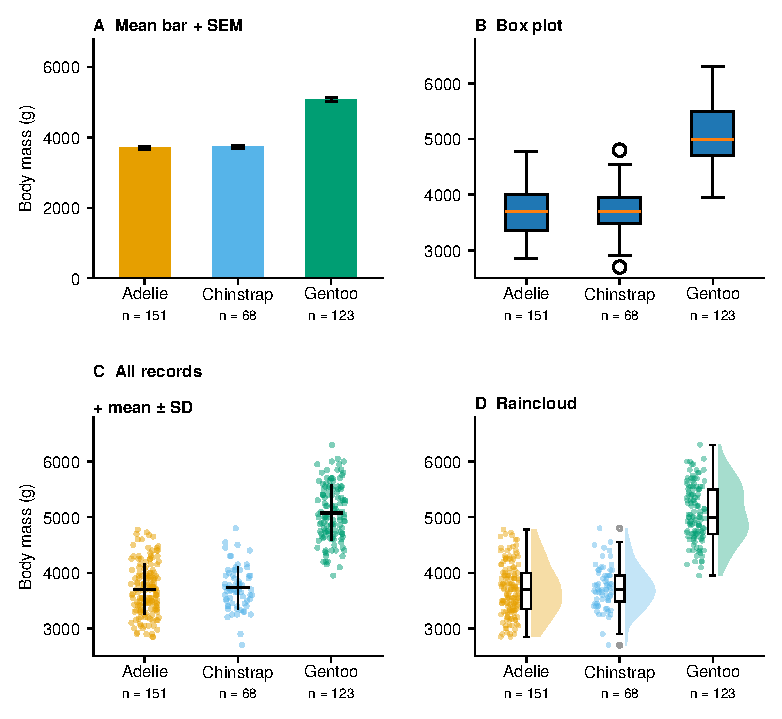
\includegraphics[width=\linewidth]{figures/ch05/ch05-01-group-forms-en.pdf}
\caption{Four views of the same data. Body mass of three penguin species (\texttt{palmerpenguins}; $n = 342$ records after removing 2 records with missing body mass). (A) Mean bars $\pm 1\ \text{SEM}$; (B) box plots with whiskers at $1.5 \times \text{IQR}$; (C) all records with group mean $\pm 1\ \text{SD}$; (D) raincloud plot combining half-violin kernel density, box plot, and jittered raw points. Panel A reduces 342 records to six summary numbers, hiding both the two-fold difference in group sizes and the shape of each distribution.}\label{fig:ch05-01}
\end{figure}

Comparing the four panels of Figure~\ref{fig:ch05-01} shows what each chart reveals or conceals:

\begin{itemize}
\item \textbf{Panel A (Mean bar + SEM): compressing 342 records into 6 numbers.} Panel A starts its vertical axis honestly at $0\ \text{g}$, yet it conveys only three group means ($3700.7\ \text{g}$, $3733.1\ \text{g}$, and $5076.0\ \text{g}$) and three SEMs ($37.3\ \text{g}$, $46.6\ \text{g}$, and $45.5\ \text{g}$). On a six-kilogram scale, the SEM whiskers shrink into tiny black caps. Without the explicit \texttt{n =} labels below the horizontal axis, three equal-width bars would hide the fact that Chinstrap ($n = 68$) has fewer than half as many records as Adelie ($n = 151$). Moreover, no adult penguin weighs between $0\ \text{g}$ and $2700\ \text{g}$, yet solid bars fill that empty zone while compressing the actual data range ($2700\text{--}6300\ \text{g}$) into the upper half of the frame. As Weissgerber et al.\ (2015) showed, identical bar graphs can conceal normal, skewed, bimodal, or outlier-driven distributions; for small-to-moderate sample sizes, authors should plot the individual points.

\item \textbf{Panel B (Box plot): exposing quartiles and extreme points while still hiding $n$ and subpopulations.} Because a box plot encodes values by vertical position rather than bar area from zero, Panel B focuses its vertical axis on $2500\text{--}6800\ \text{g}$. Orange lines mark the medians ($3700\ \text{g}$, $3700\ \text{g}$, and $5000\ \text{g}$), box edges mark the first and third quartiles (interquartile range, IQR), and whiskers extend to $1.5 \times \text{IQR}$. A feature hidden in Panel A now appears: Chinstrap has two open-circle extreme points beyond the whiskers ($2700\ \text{g}$ and $4800\ \text{g}$). However, uniform box widths still hide sample-size differences, and pooling females and males within a species merges any bimodal split into a single box.

\item \textbf{Panel C (All records + mean $\pm$ SD): returning every observation to the reader.} Panel C plots all 342 records as semi-transparent horizontally jittered points alongside a black horizontal tick (mean) and vertical bar ($\pm 1\ \text{SD}$). Three facts are immediately visible: the sky-blue Chinstrap cloud in the middle is sparser than the flanking clouds; individual weights within each species span nearly two kilograms (Adelie $2850\text{--}4775\ \text{g}$, Chinstrap $2700\text{--}4800\ \text{g}$, Gentoo $3950\text{--}6300\ \text{g}$), captured by the $\pm 1\ \text{SD}$ bars; and extreme observations sit naturally at the top and bottom of each cloud without needing arbitrary whisker cut-offs.

\item \textbf{Panel D (Raincloud plot): combining distribution contour, box plot, and raw points.} Following Allen et al.\ (2019), Panel D places horizontally jittered points on the left of each group (``rain''), a narrow white box plot in the centre, and a half-violin kernel density curve truncated at the group's minimum and maximum on the right (``cloud''). The density contour reveals internal clustering: the bluish-green Gentoo density curve on the right exhibits a broad, two-shouldered profile around $4700\ \text{g}$ and $5500\ \text{g}$, hinting at the underlying female and male subpopulations.
\end{itemize}

This leads to a clear selection rule: \textbf{for small-to-moderate group sizes (from a few observations up to a couple of hundred per group), show all raw points alongside a summary statistic (Panel C or D); when group sizes are so large that points fuse into an ink blot, use box, violin, or raincloud plots and print each group's $n$ along the axis.} When instructing \scidraw{} Scientific Visualization (\sdtool{sci-vis}) to plot raw points, specify that \textbf{random jitter must only perturb horizontal x-positions and never alter vertical values}:

\begin{Prompt}
Change the chart to a grouped strip plot: put species (Adelie, Chinstrap, Gentoo)
on the x-axis and Body mass (g) on the y-axis with range 2500 to 6800.
Plot all 342 individual records as semi-transparent points. Jitter points
horizontally only (within 15% of the group spacing) to reduce overlap; do not
alter any vertical y-values. Overlay each group's mean (horizontal tick) and
+/- 1 SD (vertical line), and print n = ... beneath each species name.
\end{Prompt}

\section{What an Error Bar Actually Means}

Compare Panels A and C of Figure~\ref{fig:ch05-01}: both summarize the same 151 Adelie records, so why is the error bar in Panel A a tiny cap of $37.3\ \text{g}$ whereas the vertical bar in Panel C spans $458.6\ \text{g}$ on each side of the mean? Because Panel A plots the standard error of the mean (SEM) and Panel C plots the sample standard deviation (SD). Confusing error-bar metrics—or omitting their definition—is a pervasive flaw in experimental papers (Cumming et al., 2007; Krzywinski and Altman, 2013).

The three common error-bar statistics answer three distinct questions (Table~\ref{tab:ch05-err}):

\begin{table}[htbp]\centering\footnotesize
\setlength{\tabcolsep}{2.5pt}
\renewcommand{\arraystretch}{1.15}
\caption{Meaning, scaling behaviour, and actual half-widths of the three common error-bar statistics on the penguin body-mass data ($n = 342$: Adelie 151, Chinstrap 68, Gentoo 123).}\label{tab:ch05-err}
\begin{tabularx}{\linewidth}{@{}>{\raggedright\arraybackslash}p{20mm}>{\raggedright\arraybackslash}p{22mm}Yccc@{}}
\toprule
\textbf{Error bar} & \textbf{Formula} & \textbf{Question answered and behaviour as $n$ grows} & \textbf{Adelie} & \textbf{Chinstrap} & \textbf{Gentoo} \\
\midrule
Sample SD & $s = \sqrt{\frac{\sum (x_i - \bar{x})^2}{n-1}}$ & \textbf{Biological spread:} How much do individual records vary around the mean? Stabilizes as $n$ grows; does not shrink with larger samples. & $458.6\ \text{g}$ & $384.3\ \text{g}$ & $504.1\ \text{g}$ \\
Standard error (SEM) & $\text{SEM} = s / \sqrt{n}$ & \textbf{Estimation precision:} How precisely does the sample mean estimate the population mean? Shrinks at rate $1/\sqrt{n}$; does not describe individual spread. & $37.3\ \text{g}$ & $46.6\ \text{g}$ & $45.5\ \text{g}$ \\
95\% CI half-width & $t_{0.975,\,n-1} \times \text{SEM}$ & \textbf{Interval estimation:} Half-width of the 95\% confidence interval for the population mean (roughly $2 \times \text{SEM}$ for moderate-to-large $n$). & $73.7\ \text{g}$ & $93.0\ \text{g}$ & $90.0\ \text{g}$ \\
\bottomrule
\end{tabularx}
\end{table}

Three rules follow from Table~\ref{tab:ch05-err}:

First, \textbf{on the same data, SD and SEM can differ by more than ten-fold.} For the 151 Adelie records, $\text{SD} = 458.6\ \text{g}$; dividing by $\sqrt{151} \approx 12.29$ gives $\text{SEM} = 37.3\ \text{g}$, and the 95\% CI half-width is $73.7\ \text{g}$. To show biological variability among individuals, plot SD (or IQR); to show uncertainty around an estimated group mean, plot the 95\% CI. Never choose SEM merely to make error bars look small.

Second, \textbf{every figure with error bars must state both the error-bar type and each group's $n$ in the legend or caption.} Only when both are given can readers interpret the bars or convert between metrics.

Third, \textbf{do not judge statistical significance by whether error bars overlap} (Cumming et al., 2007; Krzywinski and Altman, 2013). When bars show $\pm 1\ \text{SD}$, heavy overlap is still compatible with highly significant mean differences. Conversely, when independent $\pm 1\ \text{SEM}$ bars just touch without overlapping, the two-sided $p$-value is still above $0.05$ (for two independent groups of similar size, $\pm 1\ \text{SEM}$ bars need a gap of roughly $0.5\text{--}1\ \text{SEM}$, or 95\% CI bars must overlap by no more than about one-fourth of one arm, to correspond roughly to $p \le 0.05$).

Because many AI plotting tools default to drawing unlabelled SEM bars, always specify the exact metric in \sdtool{sci-vis}:

\begin{Prompt}
Use sample standard deviation (+/- 1 SD, ddof = 1) for all error bars; do not
use standard error of the mean (SEM). State "Tick: mean; line: +/- 1 SD" in
the legend, print the sample size n below each group on the x-axis, and do not
add significance asterisks or p-values.
\end{Prompt}

\section{Paired and Repeated Measures}

When two columns of numbers come from the same experimental units measured before and after a treatment—or the same sites across two periods—the rows carry a one-to-one \textbf{paired structure}. Returning to the simulated teaching dataset from Chapters 1 and 2 (\texttt{paired-example.csv}, CC BY 4.0), 8 fictional objects (\texttt{SIM01}--\texttt{SIM08}) have a pre-test mean of $13.125\ \text{a.u.}$, a post-test mean of $16.5\ \text{a.u.}$, individual differences ($\text{after} - \text{before}$) of $+4, +3, +4, -1, +4, +5, +4, +4$, and a mean difference of $3.375\ \text{a.u.}$. Figure~\ref{fig:ch05-03} compares three ways of plotting these pairs.

\begin{figure}[htbp]\centering
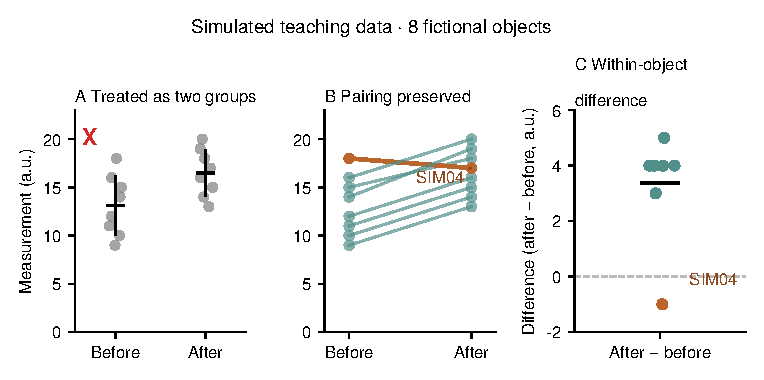
\includegraphics[width=\linewidth]{figures/ch05/ch05-03-paired-views-en.pdf}
\caption{Three ways to plot paired data (simulated teaching data). Eight fictional objects measured twice. (A) Treating the columns as independent groups discards the pairing and suggests 16 objects; (B) connecting each object's two values keeps the decrease of \texttt{SIM04} visible; (C) plotting within-object differences answers ``how much did each change'': seven positive, one negative (\texttt{SIM04} $= -1$), mean difference $3.375\ \text{a.u.}$. No significance test was performed.}\label{fig:ch05-03}
\end{figure}

Inspecting the three panels of Figure~\ref{fig:ch05-03} shows how layout choices either destroy or preserve the pairing:

\begin{itemize}
\item \textbf{Panel A (Treated as two groups, marked with a red \texttt{X}): discarding the pairing.} Panel A plots \texttt{Before} and \texttt{After} as two unlinked clouds of grey dots with mean $\pm 1\ \text{SD}$. First, 16 unlinked dots mislead readers into assuming 16 independent objects were measured. Second, wide baseline variation across objects ($9$ to $18$ before treatment) swamps the within-object change, so the two vertical clouds overlap heavily and hide whether individuals went up or down.

\item \textbf{Panel B (Pairing preserved—paired dot--line plot): exposing individual trajectories.} Panel B connects each object's \texttt{Before} and \texttt{After} values. Seven teal lines climb in parallel ($+3$ to $+5\ \text{a.u.}$), whereas a single object in warm brown—\texttt{SIM04}—starts at the highest baseline ($18$) and drops to $17$ ($-1$). Use Panel B when both initial baseline levels (such as a potential ceiling effect in \texttt{SIM04}) and individual directions of change matter.

\item \textbf{Panel C (Within-object difference plot): directly answering ``how much did each unit change?''} Panel C plots the eight differences ($\text{After} - \text{before}$) on the vertical axis, marks the mean difference ($3.375\ \text{a.u.}$) with a black horizontal tick, and draws a dashed grey reference line at $y = 0$. Seven teal dots sit above zero between $+3$ and $+5$ (the five ties at $+4$ are jittered horizontally), while \texttt{SIM04} sits below zero at $-1$. One rule is mandatory: \textbf{the vertical axis of a difference plot ($-2$ to $6$ here) must include $0$ and display a zero reference line}, because zero separates gains from losses.
\end{itemize}

When plotting paired data with AI tools, guard against two risks: first, the tool ignoring \texttt{sample\_id} and defaulting to Panel A; second, vague prompts like ``clean the data and highlight the main trend'' causing automated scripts to drop the lone decreasing unit \texttt{SIM04} as an ``outlier.'' Always specify: ``Connect observations by \texttt{sample\_id}; retain all 8 objects and never drop counter-trend or extreme observations.''

\section{Time Series and the Dual-Axis Trap}

Time-series plots rest on two rules: \textbf{the horizontal axis must map time continuously in true proportion, and interpolations or methodological changes recorded in the metadata must be marked on the plot.}

We illustrate these rules with the classic atmospheric $\text{CO}_2$ dry-air mole fraction monthly mean record from the Mauna Loa Observatory in Hawaii (Keeling, 1960; maintained by Dr.\ Xin Lan at NOAA GML and Dr.\ Ralph Keeling at Scripps Institution of Oceanography; public domain, WMO X2019 scale). Our locked snapshot (file creation date October 9, 2026) spans 823 monthly rows from March 1958 ($315.71\ \text{ppm}$) to September 2026 ($426.07\ \text{ppm}$), with a minimum monthly mean of $312.42\ \text{ppm}$ and a peak of $432.34\ \text{ppm}$ in May 2026. Figure~\ref{fig:ch05-04} shows the standard presentation of this series.

\begin{figure}[htbp]\centering
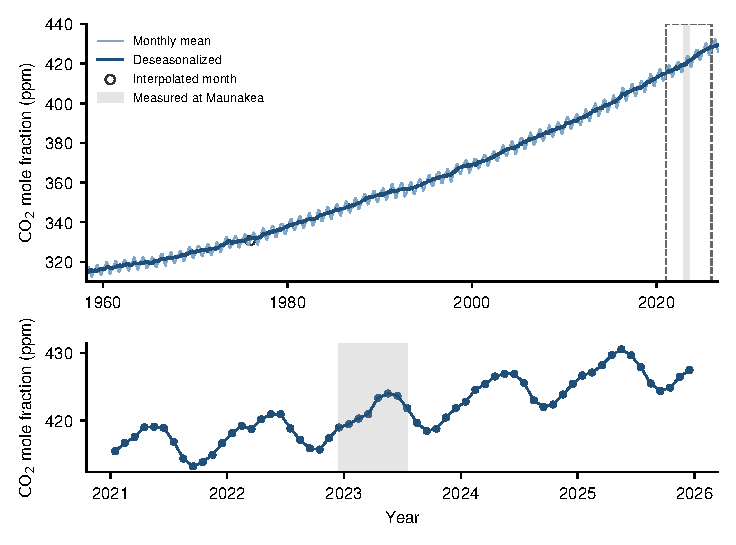
\includegraphics[width=\linewidth]{figures/ch05/ch05-04-co2-series-en.pdf}
\caption{Monthly mean atmospheric $\text{CO}_2$ at Mauna Loa, March 1958 to September 2026 snapshot. Top (full record): thin light-blue line, monthly means (\texttt{average}); thick dark-blue line, NOAA's deseasonalized trend (\texttt{deseasonalized}); open circle, the interpolated month flagged in the data notes (December 1975); grey vertical band, the period after the late-2022 eruption when measurements were made at Maunakea (December 2022--July 2023); dashed box on the right outlines the zoom window. Bottom: the last five complete calendar years (2021--2025), showing the seasonal cycle. Data: NOAA GML (X.\ Lan) and Scripps Institution of Oceanography (R.\ Keeling), snapshot dated October 9, 2026; data before May 1974 are from Scripps.}\label{fig:ch05-04}
\end{figure}

Inspecting Figure~\ref{fig:ch05-04} highlights four time-series standards:

\begin{enumerate}
\item \textbf{Continuous numerical time axis:} The horizontal axis plots \texttt{decimal date} so every month and year is spaced proportionally rather than treated as categorical text labels.
\item \textbf{Raw observations layered with official trend:} The upper panel plots both the thin light-blue monthly mean curve (\texttt{average}) and the thick dark-blue official deseasonalized curve (\texttt{deseasonalized}), without substituting an undocumented smoother.
\item \textbf{Zoomed window for high-frequency cycles:} Over nearly 70 years, seasonal oscillations compress into fine sawteeth. A dashed box on the right of the upper panel marks the last five complete years (2021--2025), expanded in the lower panel (at a $2:1$ height ratio) with monthly dots showing the Northern Hemisphere growing-season cycle (peaking around May, troughing in September--October).
\item \textbf{Marking metadata notes from \texttt{\#} header comments:} Skipping \texttt{\#} comment lines when reading a CSV hides critical provenance. The Mauna Loa header notes two special cases: first, data prior to May 1974 come from Scripps, and since NOAA began independent measurements in May 1974, December 1975 is the only month with zero valid observation days (\texttt{ndays = -1}) due to instrument failure, making its value an interpolation—marked with an open circle (\texttt{Interpolated month}); second, after the late-November 2022 eruption of Mauna Loa cut power and road access, measurements from December 2022 through July 2023 were temporarily taken at the Maunakea summit roughly 21 miles away—shaded with a light-grey vertical band (\texttt{Measured at Maunakea}) in both panels. Only an author who reads the file header can instruct the tool to flag these events.
\end{enumerate}

When comparing two time series with different units or magnitudes, the most common trap is the \textbf{dual-axis chart (twin y-axes)}. Taking the 67 complete calendar years in our snapshot (1959--2025), we compute each year's 12-month arithmetic mean concentration and then the difference between consecutive annual means for 1960--2025 (66 values in $\text{ppm yr}^{-1}$: minimum $0.42$, maximum $3.52\ \text{ppm yr}^{-1}$ in 2024; $0.93\ \text{ppm yr}^{-1}$ in 1960 and $2.74\ \text{ppm yr}^{-1}$ in 2025; note that this consecutive-annual-mean difference differs from NOAA's official December-to-December growth-rate estimator, which the caption must state). Figure~\ref{fig:ch05-06} contrasts a dual-axis plot with stacked panels.

\begin{figure}[htbp]\centering
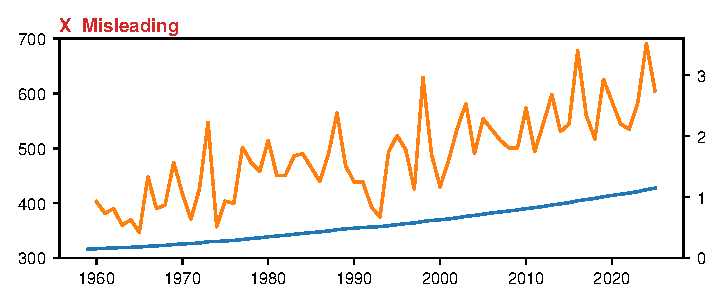
\includegraphics[width=\linewidth]{figures/ch05/ch05-06-dual-axis-bad-en.pdf}\\[4pt]
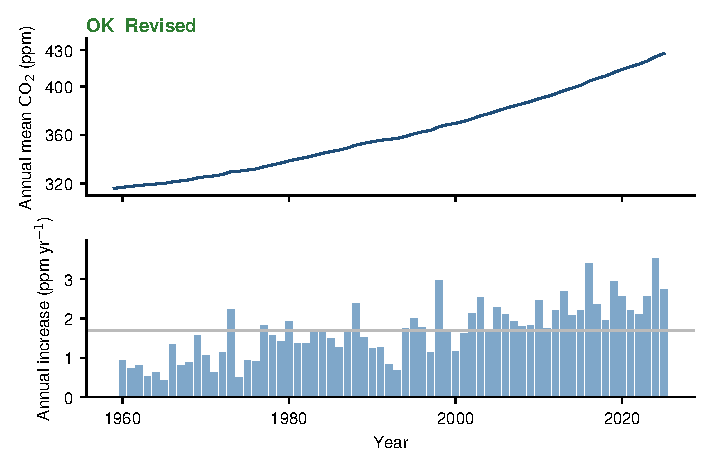
\includegraphics[width=\linewidth]{figures/ch05/ch05-06-dual-axis-good-en.pdf}
\caption{Dual axes versus stacked panels (top: deliberately misleading teaching example). Top: annual mean $\text{CO}_2$ and its annual increase share one plot with two y-axes whose ranges were chosen arbitrarily, so the visual alignment of the curves means nothing. Bottom: each quantity has its own panel on a shared time axis, and the annual increase is plotted from zero. Annual means are averages of NOAA monthly values for complete years (1959--2025); the annual increase is the difference between consecutive annual means, which differs from NOAA's published growth-rate method.}\label{fig:ch05-06}
\end{figure}

In the upper plot of Figure~\ref{fig:ch05-06} (\texttt{X Misleading}), the left axis runs from $300$ to $700\ \text{ppm}$, squashing the rising blue concentration curve against the bottom, while the right axis runs from $0$ to $3.6$ so the orange annual-increase curve fills the frame, with both axes lacking titles and units. Because \textbf{the origin and scale of two vertical axes can be chosen arbitrarily}, altering either axis range can make the two lines cross or run parallel at any year, manufacturing false visual relationships. The lower plot (\texttt{OK Revised}) gives each quantity its own panel above a shared 1959--2025 time axis: the upper panel shows annual mean $\text{CO}_2$ ($310\text{--}440\ \text{ppm}$), and the lower panel shows annual increase as a bar chart starting at $0$ ($0\text{--}4.0\ \text{ppm yr}^{-1}$) with a light-grey reference line at the 1960--2025 mean ($1.69\ \text{ppm yr}^{-1}$).

\section{Scatter Plots and Correlation: When Grouping Flips the Answer}

When examining two continuous variables, omitting categorical grouping variables often leads AI tools to fit a single pooled regression line across all rows—a default that can reverse the scientific conclusion. Figure~\ref{fig:ch05-08} uses penguin bill length (\texttt{bill\_length\_mm}) and bill depth (\texttt{bill\_depth\_mm}, $n = 342$ after removing 2 missing rows) to demonstrate \textbf{Simpson's paradox}.

\begin{figure}[htbp]\centering
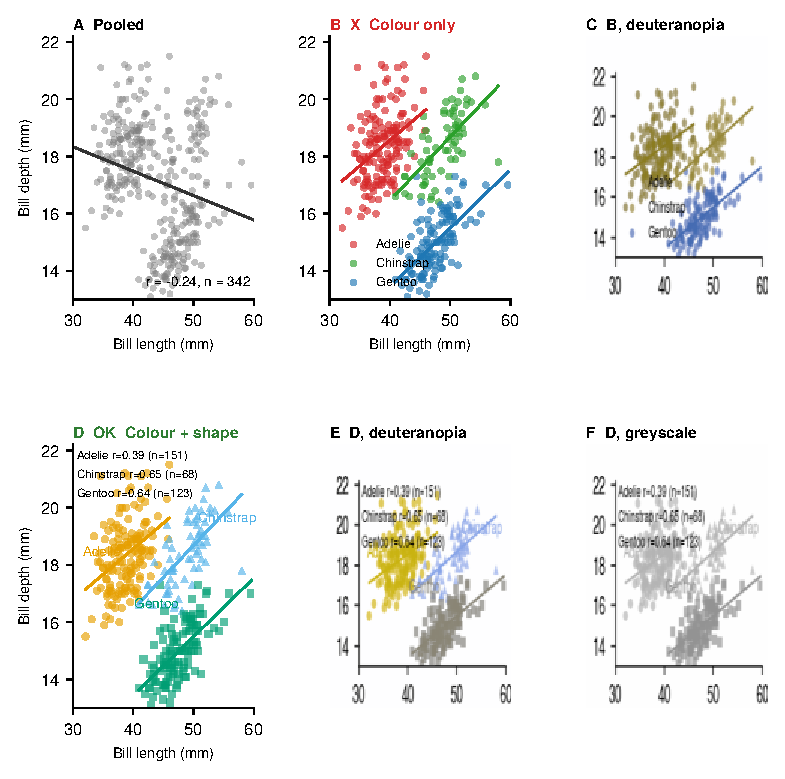
\includegraphics[width=\linewidth]{figures/ch05/ch05-08-scatter-cvd-en.pdf}
\caption{Grouping can reverse a correlation, and group colours must survive checking. Penguin bill length versus bill depth ($n = 342$ records). (A) Pooled, the correlation is negative ($r = -0.24$); (B, D) within each species it is positive ($r = 0.39$, $0.65$, and $0.64$). In (B), species differ only by red, green, and blue circles and become hard to tell apart under simulated deuteranopia (C; Machado et al.\ 2009 model). (D) uses a colour-blind-safe palette, distinct marker shapes, and direct labels, which remain legible under simulation (E) and in greyscale (F). Lines are ordinary least-squares fits, shown descriptively.}\label{fig:ch05-08}
\end{figure}

Compare Panel A and Panel D of Figure~\ref{fig:ch05-08}. In \textbf{Panel A (\texttt{A Pooled})}, all 342 records are mixed into a single cloud of grey dots, and the ordinary least-squares (OLS) line slopes downward ($r = -0.24$, $n = 342$), suggesting that longer bills are shallower.

In \textbf{Panels B and D}, stratifying those same 342 records by species reverses the correlation by 180 degrees: within every species, bill length and depth are positively correlated—Adelie $r = 0.39$ ($n = 151$, upper-left orange circles), Chinstrap $r = 0.65$ ($n = 68$, upper-right sky-blue triangles), and Gentoo $r = 0.64$ ($n = 123$, lower-right bluish-green squares). Panel D shows why: large-bodied Gentoo penguins have relatively long, shallow bills (lower right), whereas Adelie penguins have shorter, deeper bills (upper left); within each species, larger individuals have both longer and deeper bills. The pooled line in Panel A merely connects the centroids of distinct species clusters, mistaking \textbf{between-species divergence} for \textbf{within-species allometry}.

When directing AI tools to make scatter plots, enforce three rules: (1) declare grouping variables up front rather than accepting a pooled fit; (2) report $r$ together with $n$ and the grouping level (as in Panel D) and state the fitting method in the caption; and (3) do not clutter exploratory plots with unadjusted regression $p$-values.

\section{Keeping Charts Honest: Truncated Axes, 3D Bars, Excess Decimals, and Rainbow Colormaps}

Four additional errors frequently distort quantitative charts: \textbf{truncated bar axes, 3D perspective bars, false decimal precision, and rainbow colormaps.}

Figure~\ref{fig:ch05-05} uses the three species mean body masses ($n = 342$) to contrast a chart combining the first three flaws (left) with an honest dot plot of the same values (right).

\begin{figure}[htbp]\centering
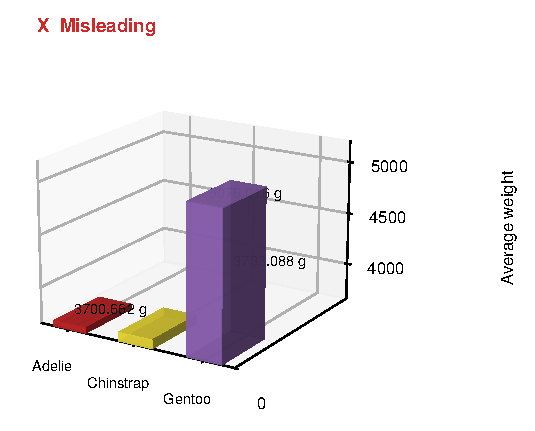
\includegraphics[width=0.49\linewidth]{figures/ch05/ch05-05-axis-bad-en.pdf}\hfill
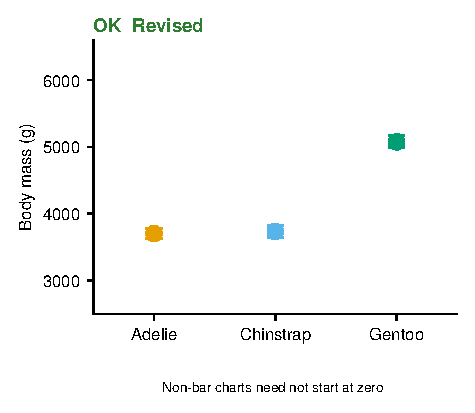
\includegraphics[width=0.49\linewidth]{figures/ch05/ch05-05-axis-good-en.pdf}
\caption{A misleading and an honest view of the same means (deliberately bad example on the left). Left: 3D bars, an axis truncated at $3650\ \text{g}$, rainbow colours, three decimal places, and no unit make a $<1\%$ difference between Adelie and Chinstrap look dramatic. Right: means with 95\% confidence intervals on a labelled axis with integer ticks. Data as in Figure~\ref{fig:ch05-01} ($n = 342$).}\label{fig:ch05-05}
\end{figure}

Inspecting the left panel of Figure~\ref{fig:ch05-05} (\texttt{X Misleading}) reveals three concrete defects:

\begin{enumerate}
\item \textbf{Truncating a bar chart's axis magnifies tiny differences:} Bar charts encode value by bar height and area from a zero baseline, so their axis must start at $0$. Cropping the axis at $3650\ \text{g}$ turns a $32.4\ \text{g}$ difference between Adelie ($3700.7\ \text{g}$) and Chinstrap ($3733.1\ \text{g}$)—less than $0.9\%$—into visible bar heights of $50.7\ \text{g}$ versus $83.1\ \text{g}$ (over 60\% taller), while the purple Gentoo bar ($5076.0\ \text{g}$) towers overhead. The right panel (\texttt{OK Revised}) switches to a \textbf{2D dot plot of means and 95\% CIs}: because dot plots encode value by coordinate position rather than bar area, the vertical axis can span $2500\text{--}6600\ \text{g}$ (as noted at the bottom: \texttt{Non-bar charts need not start at zero}), showing at a glance that Adelie and Chinstrap have nearly identical means with overlapping confidence intervals.
\item \textbf{3D perspective bars distort reading and cause label collisions:} In the 3D plot (\texttt{bar3d}), tilted bar tops make it impossible to tell whether to align the front or back edge with the ticks ($4000, 4500, 5000$) on the right wall; a meaningless \texttt{0} tick appears on the depth axis at bottom right; the vertical title \texttt{Average weight} is pushed to the right margin; and the floating labels \texttt{5076.016 g} and \texttt{3733.088 g} collide with the purple Gentoo bar.
\item \textbf{Excess decimals fabricate precision and units are missing:} Field weights were recorded to the nearest $25\ \text{g}$ or $50\ \text{g}$, yet the left panel prints three decimal places (\texttt{3700.662 g}) and omits units on the axis; the right panel drops redundant in-plot digits and labels the axis \texttt{Body mass (g)} with integer ticks.
\end{enumerate}

The fourth error is the \textbf{rainbow colormap (\texttt{jet})} on continuous matrices. Figure~\ref{fig:ch05-07} arranges Mauna Loa monthly mean $\text{CO}_2$ across 1959--2025 into a $67 \times 12$ matrix ($312.42\text{--}432.34\ \text{ppm}$, unsmoothed) and compares \texttt{jet} with the perceptually uniform colormap \texttt{viridis}.

\begin{figure}[htbp]\centering
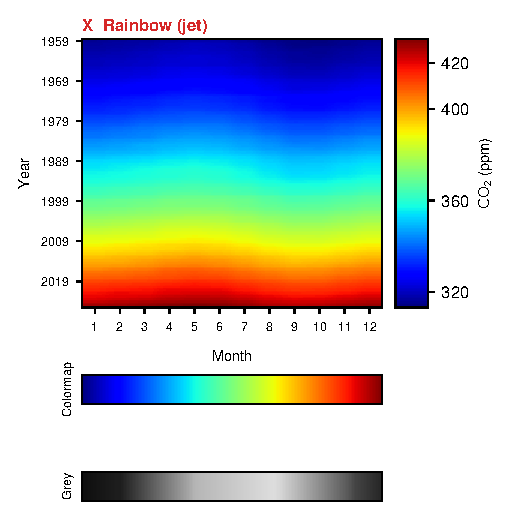
\includegraphics[width=0.49\linewidth]{figures/ch05/ch05-07-colormap-bad-en.pdf}\hfill
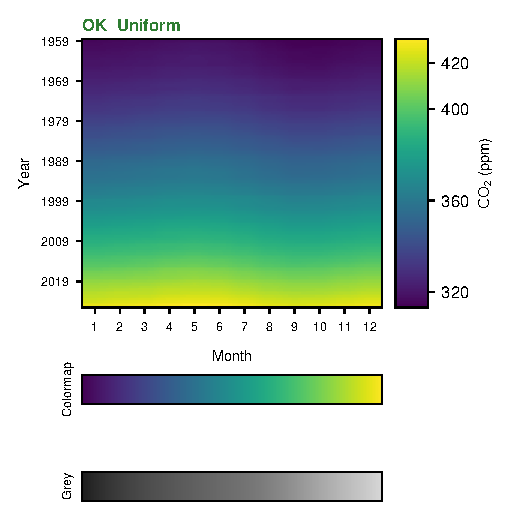
\includegraphics[width=0.49\linewidth]{figures/ch05/ch05-07-colormap-good-en.pdf}
\caption{Rainbow versus perceptually uniform colour maps (left: deliberately bad example). Both heat maps show the same $67 \times 12$ matrix of monthly mean $\text{CO}_2$ at Mauna Loa, 1959--2025. The \texttt{jet} map introduces apparent boundaries at cyan and yellow that are not in the data, and its greyscale strip (\texttt{Grey}) rises then falls in lightness; \texttt{viridis} increases monotonically in lightness and still reads correctly in greyscale.}\label{fig:ch05-07}
\end{figure}

In Figure~\ref{fig:ch05-07}, even though $\text{CO}_2$ rises smoothly over 67 years, the left heatmap (\texttt{X Rainbow (jet)}) creates false sharp bands at bright cyan (around 1989) and bright yellow (around 2009). Worse, its bottom \texttt{Grey} strip shows that luminance in \texttt{jet} rises in the middle and darkens at both ends (deep blue and deep red), scrambling low and high values when printed in black and white (Crameri et al., 2020; Nu\~nez et al., 2018). The right panel (\texttt{OK Uniform}) uses \texttt{viridis} (or \texttt{cividis} for severe colour-vision deficiency), whose \texttt{Grey} strip brightens monotonically from left to right, preserving both the long-term rise and the May-peak / autumn-trough seasonal wave in greyscale.

To fix these flaws in \sdtool{sci-vis}, send a direct prompt:

\begin{Prompt}
1. Replace the 3D bar chart with a 2D plot of group means and 95% confidence
   intervals (if using bars, the y-axis must start at 0). Never use 3D bars.
   Remove the 3-decimal text labels, title the y-axis "Body mass (g)", and use
   integer tick marks.
2. For the heatmap, replace the rainbow (jet) colormap with the perceptually
   uniform colormap viridis (or cividis), and label the colorbar "CO2 (ppm)".
\end{Prompt}

\section{Checking for Colour-Vision Deficiency and Greyscale}

Roughly 8\% of men of Northern European descent have some form of red--green colour-vision deficiency (most commonly deuteranopia or deuteranomaly), and many readers across all populations are affected (Wong, 2011)—and papers are frequently read in greyscale printouts. Categorical groups must never rely on red-versus-green hue alone.

Return to Panels B--F of Figure~\ref{fig:ch05-08}. \textbf{Panel B (\texttt{B X Colour only})} plots all three species as identical circles distinguished only by red, green, and blue. Under physiological deuteranopia simulation (Machado et al., 2009) in \textbf{Panel C (\texttt{C B, deuteranopia})}, the red Adelie and green Chinstrap clouds, regression lines, and legend markers collapse into nearly indistinguishable olive-brown tones. By contrast, \textbf{Panel D (\texttt{D OK Colour + shape})} combines three defences: (1) the Okabe--Ito palette (\texttt{\#E69F00}, \texttt{\#56B4E9}, \texttt{\#009E73}); (2) \textbf{redundant marker shapes} (circles \texttt{o} for Adelie, triangles \texttt{\^{}} for Chinstrap, squares \texttt{s} for Gentoo); and (3) \textbf{direct species labels} beside each cloud (note also that at final print scale one should check label placement—in Panel D the correlation text at upper left sits near the highest Adelie circles and the direct species names sit snug against the clouds, which can be nudged if needed). With this triple encoding, all three groups remain clear under simulated deuteranopia (\textbf{Panel E}) and in greyscale (\textbf{Panel F}).

Before submission, upload exported figures to \scidraw{} Figure Checker (\sdtool{figure-checker}) for automated greyscale and colour-vision simulation checks—remembering that technical checks never replace scientific review (such as catching Simpson's paradox in Panel A).

\section{End-to-End Case Study: Completing a Penguin Body-Mass Figure with SciDraw AI}

We now complete Lin Yue's opening task: using \path{penguins.csv}, build a figure for the ``Study System'' subsection and lab-meeting slides showing adult breeding body mass across the three \emph{Pygoscelis} species (Adelie \emph{P.\ adeliae}, Chinstrap \emph{P.\ antarcticus}, Gentoo \emph{P.\ papua}) stratified by species and sex. First, we fix the scientific boundary: \textbf{this figure is a purely descriptive morphological display; no inferential statistical tests are run, and no asterisks or $p$-values are drawn.}

\textbf{Step 1: Independently compute benchmark values.} Following Table~\ref{tab:ch05-dict}, dropping the 11 rows where \texttt{sex} or \texttt{body\_mass\_g} is \texttt{NA} leaves \textbf{$n = 333$} records. Before using AI, we compute the sample size, mean, and sample SD ($\text{ddof} = 1$) for all six species $\times$ sex subgroups (Table~\ref{tab:ch05-case-expect}; pooled species values are in Table~\ref{tab:ch05-err}). Comparing the two tables shows that within every species, males average $412\text{--}805\ \text{g}$ heavier than females, and within-sex SDs ($269.4\text{--}362.1\ \text{g}$) are much smaller than pooled-sex SDs ($384.3\text{--}504.1\ \text{g}$), confirming that much of the pooled spread comes from sexual dimorphism.

\begin{table}[htbp]\centering\footnotesize
\setlength{\tabcolsep}{4pt}
\renewcommand{\arraystretch}{1.15}
\caption{Verification benchmark table of penguin body mass by species $\times$ sex (excluding 11 rows with missing sex or body mass; $n = 333$).}\label{tab:ch05-case-expect}
\begin{tabularx}{\linewidth}{@{}llccY@{}}
\toprule
\textbf{Species (common and scientific name)} & \textbf{Sex} & \textbf{Records $n$} & \textbf{Mean (g)} & \textbf{Sample SD (g)} \\
\midrule
Adelie (\emph{P.\ adeliae}) & \texttt{female} & 73 & 3368.8 & 269.4 \\
Adelie (\emph{P.\ adeliae}) & \texttt{male}   & 73 & 4043.5 & 346.8 \\
Chinstrap (\emph{P.\ antarcticus}) & \texttt{female} & 34 & 3527.2 & 285.3 \\
Chinstrap (\emph{P.\ antarcticus}) & \texttt{male}   & 34 & 3939.0 & 362.1 \\
Gentoo (\emph{P.\ papua}) & \texttt{female} & 58 & 4679.7 & 281.6 \\
Gentoo (\emph{P.\ papua}) & \texttt{male}   & 61 & 5484.8 & 313.2 \\
\bottomrule
\end{tabularx}
\end{table}

\textbf{Step 2: Draft the figure brief in the Figure Workflow Guide.} In \scidraw{} Figure Workflow Guide (\sdtool{figure-workflow}), select the ``Data Figure'' route, replace the default brief with the specification below, download a copy, and proceed to Scientific Visualization (\sdtool{sci-vis}):

\begin{Prompt}
[Research Question] How does adult body mass distribute across three Pygoscelis
                    penguin species, and how much do females and males differ
                    within each species?
[Purpose & Audience] Descriptive figure for the paper's "Study System" section
                     (single-column width ~85 mm) plus lab-meeting slides;
                     audience is ecology peers.
[Data Source] Public dataset: penguins.csv from palmerpenguins v0.1.0 (CC0),
              Palmer Station LTER, 2007-2009.
[Fields & Units] species (group), sex (subgroup), body_mass_g (Body mass, g).
[Unit of Observation & n] Each row is one measurement record. Exclude the 11 rows
              where sex or body_mass_g is NA, retaining n = 333 records. Print
              each subgroup's n beneath the x-axis.
[Pairing] None. Records are unlinked; do not connect points with lines.
[Visual Encoding] Grouped strip plot: arrange species as Adelie, Chinstrap,
              Gentoo; place female on the left and male on the right within each.
[Summary & Error Bars] Show all raw points (jittered horizontally only; y-values
              unchanged). Overlay group mean +/- 1 SD. No tests, asterisks, or p.
[Forbidden Operations] Do not fabricate, drop, or alter values; do not remove
              "outliers" or impute missing rows.
[Labels & Export] Y-axis "Body mass (g)" with integer ticks; open circles for
              females, filled circles for males; colour-blind-safe species palette;
              legend stating "Tick: mean; line: +/- 1 SD". Export PNG and PDF.
[Acceptance] Subgroup n = 73, 73, 34, 34, 58, 61; means match benchmark table.
\end{Prompt}

\textbf{Step 3: Upload data and audit the first draft.} In Scientific Visualization (\sdtool{sci-vis}), upload \path{penguins.csv} (supports CSV, TSV, TXT, XLSX, XLS, and pasted tables; Excel reads only the first worksheet) and confirm that the interface reports 344 rows $\times$ 8 columns. The platform checks the file hash, byte size, and row count and lets you download the stored raw file to verify that the plot uses your exact table—\textbf{but file integrity does not guarantee appropriate statistical choices.} Paste the brief requirements to generate the first draft, then check it against Table~\ref{tab:ch05-case-expect} for five typical first-draft issues: (1) mean bars + unspecified error bars (often SEM); (2) sexes pooled, or \texttt{sex = NA} plotted as a third sex group \texttt{"NA"}; (3) bar axis truncated above zero; (4) mean labels with 1--3 decimals; and (5) red/green or default colours without open/filled sex markers.

\textbf{Step 4: Issue step-by-step revision prompts and use version rollback.} Address one category of issue per conversational turn. First, send Revision Prompt M1 (chart type and NA filtering):

\begin{Prompt}
Switch to a strip plot where each point represents one measurement record. Order
the x-axis as Adelie, Chinstrap, Gentoo, with females on the left and males on
the right within each species. Jitter points horizontally only (width no more
than 15% of the group spacing) without changing any y-values. Exclude rows where
sex or body_mass_g is NA so no "NA" group appears. Draw no bars; keep all other
settings unchanged.
\end{Prompt}

Second, send Revision Prompt M2 (summary overlay and sample-size labels):

\begin{Prompt}
To the right of each subgroup point cloud, overlay a short horizontal tick for
the group mean and a vertical line for mean +/- 1 SD (sample standard deviation,
ddof = 1). Beneath the x-axis, print each subgroup's sample size (for example,
"n = 73"). In the legend, state "Tick: mean; line: +/- 1 SD". Do not add
significance asterisks, p-values, or test results. Change only these items.
\end{Prompt}

Third, send Revision Prompt M3 (axis settings, integer ticks, and colour-blind-safe palette):

\begin{Prompt}
Set the y-axis title to "Body mass (g)" with range 2500 to 6500, tick interval
500, and integer tick labels (no decimals). Use a colour-blind-safe palette by
species: Adelie orange #E69F00, Chinstrap sky blue #56B4E9, Gentoo bluish green
#009E73; use open circles for females and filled circles for males. Do not alter
the species order or any data values.
\end{Prompt}

Note: conversational editing does not lock unmentioned elements. If M3 inadvertently alters the species order or point positions, do not pile patch prompts onto the broken chart—click ``Restore Previous Version'' (or select the prior state from the ``History'' sidebar) and split M3 into two narrower prompts (first axis settings, then palette and markers). Always re-check unmentioned elements after every turn.

\textbf{Step 5: Final verification, caption, and deliverable folder.} The platform renders charts via a declarative engine or Python backend; the current UI does not provide full script downloads, and declarative PDF/EPS exports may wrap raster content (do not assume every PDF is an editable vector graphic; native Excel chart export is available for supported chart types). We therefore cross-check the reference final figure (Figure~\ref{fig:ch05-02}) against Table~\ref{tab:ch05-case-expect}: x-axis ordered Adelie, Chinstrap, Gentoo; within each species, females on the left (open circles) and males on the right (filled circles), jittered horizontally only; black horizontal ticks and vertical lines to the right of each cloud matching the benchmark means $\pm 1\ \text{SD}$; and two rows of sample sizes beneath each species name (upper row for left/female groups: $n = 73, 34, 58$; lower row for right/male groups: $n = 73, 34, 61$, totaling $333$ with no \texttt{NA} group).

\begin{figure}[htbp]\centering
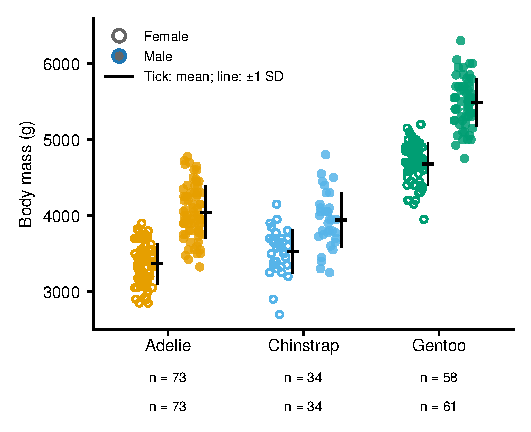
\includegraphics[width=0.68\linewidth]{figures/ch05/ch05-02-case-final-en.pdf}
\caption{Body mass of adult \emph{Pygoscelis} penguins by species and sex. Each point is one measurement record (Palmer Station LTER, 2007--2009; \texttt{palmerpenguins} v0.1.0, CC0). After excluding 11 records with missing sex or body mass, $n = 333$; group sizes are shown beneath the axis (upper row: females; lower row: males). Horizontal ticks show means and vertical lines $\pm 1\ \text{SD}$ (sample standard deviation). Points are jittered horizontally only; values are unchanged. Descriptive display; no statistical tests were performed.}\label{fig:ch05-02}
\end{figure}

If \sdtool{figure-legend} is used to draft a caption, the author must supply the data source and licence, $n = 333$ after excluding 11 missing records, the mean $\pm 1\ \text{SD}$ definition, horizontal-only jitter, and the note that no statistical tests were performed. Archive all deliverables in a structured folder (the example figures in this chapter were generated by deterministic scripts; prompts and verification records are available in the book repository):

\begin{Prompt}
penguin-mass-figure/
  source/   penguins.csv, penguins-README.md, SHA-256.txt
  brief/    figure-brief.txt, data-dictionary.md, benchmark-table.csv
  drafts/   scivis-v1.png ... scivis-v4.png, revision-prompts.md (inputs + audit notes)
  check/    independent verification output check.json, figure-checker report
  final/    figure-5-2.png, figure-5-2.pdf, caption-zh.txt, caption-en.txt, ai-usage.txt
\end{Prompt}

\section{What AI Can and Cannot Do at This Stage}

Table~\ref{tab:ch05-02} summarizes what AI visualization tools can and cannot do, and what the author must verify.

\begin{table}[htbp]\centering\footnotesize
\setlength{\tabcolsep}{3pt}
\renewcommand{\arraystretch}{1.12}
\caption{What AI can do, what it cannot do, and what the author must verify across the data-visualization workflow.}\label{tab:ch05-02}
\begin{tabularx}{\linewidth}{@{}>{\raggedright\arraybackslash}p{19mm}YYY@{}}
\toprule
\textbf{Stage} & \textbf{What AI (\scidraw{} \sdtool{sci-vis}) can do} & \textbf{Cannot do / do not delegate} & \textbf{What the author must verify} \\
\midrule
Reading data & Parse CSV/TSV/TXT/XLSX/XLS and pasted tables; verify hash, byte size, and row count & Know which rows belong to the same individual or which column is a pairing key; infer why values are missing; Excel reads only the first sheet & Row count, column names, and \texttt{NA} counts match the raw file; unit of observation is written in the brief \\
Choosing a chart & Draw strip, box, dot--line, line, or heatmap charts on command; suggest candidates & Understand study design (independent, paired, repeated) unless told; UI does not show rationale for chart suggestions & Chart type matches study design; raw points are shown whenever sample size permits \\
Summaries \& error bars & Compute and plot means, SD, SEM, and CIs & Decide which error bar is scientifically appropriate; guarantee statistical test validity & Error-bar type is stated in legend and caption; $n$ matches the plot; no unrequested asterisks or $p$-values \\
Multi-turn editing & Change chart type, labels, colours, and axes in chat; branch from history; restore previous version & Guarantee that unmentioned elements stay untouched; lock individual canvas objects & After every turn, re-check unmentioned elements (order, values, axis range) \\
Colour \& legibility & Apply specified palettes and column-width styles; run greyscale and CVD simulations in \sdtool{figure-checker} & Judge whether colours carry scientific meaning; technical checks are not scientific review & Groups remain distinct under CVD simulation and greyscale; colormap fits data type \\
Exporting & Download PNG, TIFF, PDF, EPS, and stored raw data; export native Excel charts for supported types & Provide full plotting code downloads in current UI; PDF/EPS is not always an editable vector file & Inspect exported dimensions, fonts, and vector vs.\ raster status; match raw-data hash to local file \\
Figure captions & \sdtool{figure-legend} drafts a layout description from image pixels & Know $n$, exclusion rules, error-bar meaning, or data source (it only sees pixels) & Supply data source, $n$, missing-data handling, error-bar type, and whether tests were run \\
\bottomrule
\end{tabularx}
\end{table}

\section{Chapter Checklist}

\begin{itemize}
\item What each row represents is written in the figure brief; ``number of records'' and ``number of individuals'' are not conflated.
\item Missing-value handling is stated explicitly; no \texttt{"NA"} group appears on the plot; excluded row counts are reported in the caption.
\item Chart type matches the study design: paired data preserve pairing links, time axes are continuous numbers, and grouping variables are visible.
\item When group sizes are small to moderate ($n \le$ a few dozen), all raw points are shown and jitter is strictly horizontal.
\item Error-bar type (SD / SEM / 95\% CI) is written in the legend or caption, and $n$ matches the plot.
\item Bar-chart vertical axes start at $0$; non-bar axis ranges are justified and do not exaggerate differences.
\item There are no dual y-axes, 3D bars, or false decimal places.
\item Continuous data use a perceptually uniform colormap; group colours pass colour-vision and greyscale checks with shape or label redundancy.
\item Every number on the plot has been cross-checked against an independent calculation (script or spreadsheet).
\item Saved in the archive: raw data and its hash, figure brief, every prompt and screenshot, final files, caption, and verification log.
\item Simulated data are labelled as ``simulated teaching data'' on the plot or in the caption.
\end{itemize}

\section{Exercises}

\begin{enumerate}
\item \textbf{Reading a table and choosing a chart (pen and paper):} Given \path{flipper_length_mm} and \texttt{island} in Palmer Penguins, write a data dictionary (including \texttt{NA} counts), tabulate the species composition on each island (Torgersen: 52 Adelie; Biscoe: 44 Adelie $+$ 124 Gentoo; Dream: 56 Adelie $+$ 68 Chinstrap), explain why ``comparing flipper length across the three islands'' is confounded with species (Gentoo occurs only on Biscoe, Chinstrap only on Dream), and propose a non-misleading chart (for example, faceting by island and colouring by species).
\item \textbf{Hands-on practice in \scidraw{}:} Upload \texttt{paired-example.csv} to \sdtool{sci-vis}, first enter only ``Make a before-and-after comparison chart,'' and record the first draft; then follow the logic of Figure~\ref{fig:ch05-03} through chat prompts to obtain both a paired dot--line plot and a difference plot (with vertical axis including $0$), using ``Restore Previous Version'' at least once. Submit: each prompt, screenshot, and a verification table checking all 8 differences (\texttt{SIM04} $= -1$).
\item \textbf{Fixing a misleading chart:} Using this chapter's $\text{CO}_2$ snapshot, create a flawed ``rainbow colormap + dual y-axis'' chart, then write three revision prompts that could be sent directly to an AI tool to fix it; explain how you confirm that the underlying values did not change after revision (for example, by cross-checking an annual-mean table).
\end{enumerate}

\section*{References}

\begin{itemize}
\item Allen M, Poggiali D, Whitaker K, Marshall TR, Kievit RA. Raincloud plots: a multi-platform tool for robust data visualization. \emph{Wellcome Open Research}. 2019;4:63. \url{https://doi.org/10.12688/wellcomeopenres.15191.1}
\item ColorBrewer 2.0: color advice for cartography and scientific visualization. \url{https://colorbrewer2.org/}
\item Crameri F, Shephard GE, Heron PJ. The misuse of colour in science communication. \emph{Nature Communications}. 2020;11:5444. \url{https://doi.org/10.1038/s41467-020-19160-7}
\item Cumming G, Fidler F, Vaux DL. Error bars in experimental biology. \emph{Journal of Cell Biology}. 2007;177(1):7--11. \url{https://doi.org/10.1083/jcb.200611141}
\item Gorman KB, Williams TD, Fraser WR. Ecological sexual dimorphism and environmental variability within a community of Antarctic penguins (genus \emph{Pygoscelis}). \emph{PLoS ONE}. 2014;9(3):e90081. \url{https://doi.org/10.1371/journal.pone.0090081}
\item Horst AM, Hill AP, Gorman KB. palmerpenguins: Palmer Archipelago (Antarctica) penguin data (v0.1.0) [R package]. Zenodo; 2020. \url{https://doi.org/10.5281/zenodo.3960218}
\item Keeling CD. The concentration and isotopic abundances of carbon dioxide in the atmosphere. \emph{Tellus}. 1960;12(2):200--203. \url{https://doi.org/10.3402/tellusa.v12i2.9366}
\item Krzywinski M, Altman N. Points of significance: error bars. \emph{Nature Methods}. 2013;10(10):921--922. \url{https://doi.org/10.1038/nmeth.2659}
\item Lan X, Keeling R. Trends in atmospheric carbon dioxide: Mauna Loa monthly mean data. NOAA Global Monitoring Laboratory and Scripps Institution of Oceanography. \url{https://gml.noaa.gov/ccgg/trends/data.html}
\item Machado GM, Oliveira MM, Fernandes LAF. A physiologically-based model for simulation of color vision deficiency. \emph{IEEE Transactions on Visualization and Computer Graphics}. 2009;15(6):1291--1298. \url{https://doi.org/10.1109/TVCG.2009.113}
\item Nu\~nez JR, Anderton CR, Renslow RS. Optimizing colormaps with consideration for color vision deficiency to enable accurate interpretation of scientific data. \emph{PLoS ONE}. 2018;13(7):e0199239. \url{https://doi.org/10.1371/journal.pone.0199239}
\item Okabe M, Ito K. Color Universal Design (CUD): how to make figures and presentations that are friendly to colorblind people. \url{https://jfly.uni-koeln.de/color/}
\item Rougier NP, Droettboom M, Bourne PE. Ten simple rules for better figures. \emph{PLoS Computational Biology}. 2014;10(9):e1003833. \url{https://doi.org/10.1371/journal.pcbi.1003833}
\item Weissgerber TL, Milic NM, Winham SJ, Garovic VD. Beyond bar and line graphs: time for a new data presentation paradigm. \emph{PLOS Biology}. 2015;13(4):e1002128. \url{https://doi.org/10.1371/journal.pbio.1002128}
\item Wong B. Points of view: color blindness. \emph{Nature Methods}. 2011;8(6):441. \url{https://doi.org/10.1038/nmeth.1618}
\end{itemize}

% TODO: Pending live UI and iterative session screenshots from SciDraw AI Scientific Visualization (/sci-vis) (not yet on disk, so omitted from the main text):
% - figures/ch05/ch05-scivis-v1.png (initial draft screenshot in /sci-vis)
% - figures/ch05/ch05-scivis-v2.png ... ch05-scivis-v4.png (multi-turn conversational edits and version-restore screenshots)

\chapter{Method and Workflow Diagrams}

Dr.\ Chen, a postdoctoral fellow in tumor immunology, is preparing a manuscript on a murine model of pulmonary inflammation profiled by droplet-based single-cell RNA sequencing (scRNA-seq). For Figure 1A of the paper, she needs an experimental and computational workflow diagram that shows readers across molecular biology and immunology—many of whom have never run a single-cell pipeline themselves—how fresh lung tissue from control and treated mice is transformed step by step into an annotated cell atlas.

She opens an image-generation tool and types a single sentence:

\begin{Prompt}
Create a professional, colorful flowchart of a single-cell RNA sequencing experiment and
data analysis workflow, from tissue to cell type annotation. Landscape 16:9.
\end{Prompt}

Less than a minute later, an eleven-panel color infographic appears on her screen (Figure~\ref{fig:ch06-01}). At first glance it looks polished: a dark-blue title banner spans the top, gradient headers separate the wet-lab workflow from bioinformatics analysis, and the canvas is filled with test tubes, a microfluidic channel, a benchtop sequencer, violin plots, and scatter plots.

\begin{figure}[htbp]\centering
\begin{tikzpicture}
\definecolor{ChSixBad}{HTML}{C0392B}
\node[anchor=south west,inner sep=0] (img) at (0,0) {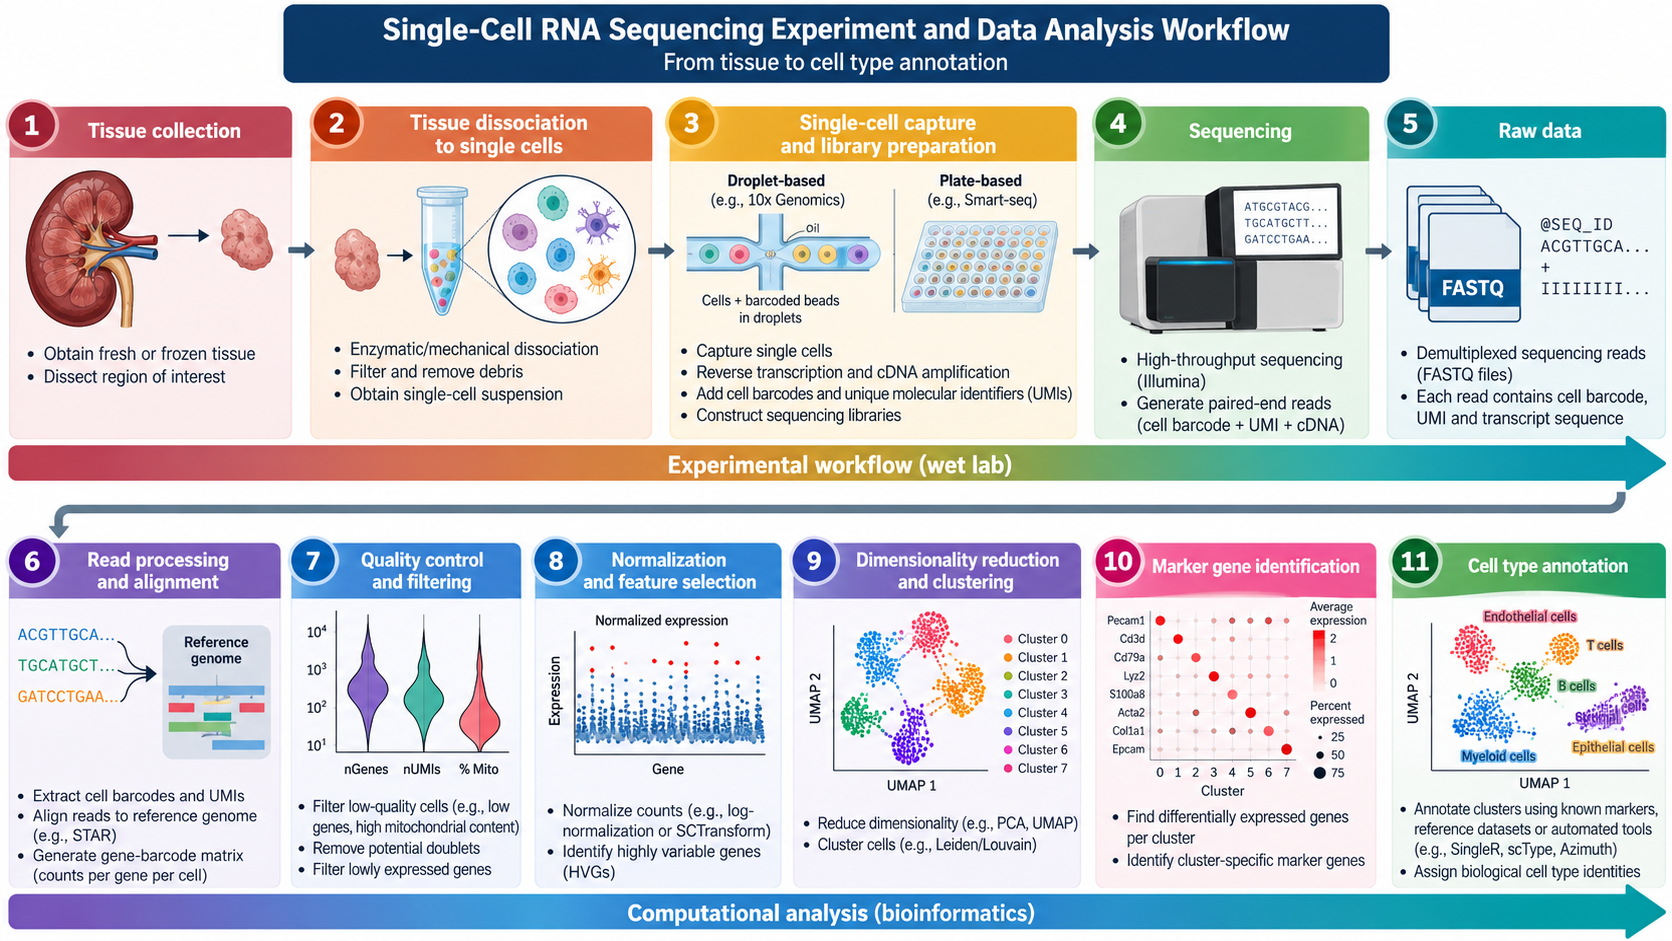
\includegraphics[width=\linewidth]{figures/ch06/ch06-01-v1-vague.png}};
\begin{scope}[x={(img.south east)},y={(img.north west)}]
  \tikzset{badmark/.style={draw=white,line width=0.8pt,fill=ChSixBad,text=white,circle,font=\sffamily\bfseries\scriptsize,inner sep=1.1pt,minimum size=4.2mm}}
  \node[badmark] at (0.09,0.74) {1};
  \node[badmark] at (0.36,0.80) {2};
  \node[badmark] at (0.91,0.78) {3};
  \node[badmark] at (0.24,0.36) {4};
  \node[badmark] at (0.55,0.36) {5};
  \node[badmark] at (0.91,0.28) {6};
\end{scope}
\end{tikzpicture}
\caption{First draft of a single-cell sequencing workflow diagram generated from a one-sentence prompt (teaching example of failure). Numbered problems: (1) top left draws a single kidney rather than lung tissue and shows only a single-sample path instead of parallel control and treated samples; (2) the wet-lab row omits cell-viability and library quality-control gates, mixes droplet-based (10x Genomics) and plate-based (Smart-seq) chemistries in panel 3, and leaves out sample pooling; (3) panel 5 frames the data product FASTQ as an operational step on par with sequencing; (4) panel 7 draws computational quality control as an ordinary inline panel with no pass or fail exits; (5) panel 9 collapses dimensionality reduction, neighbor-graph construction, clustering, and UMAP into a single panel without showing the fork from the neighbor graph to clustering versus visualization; (6) the endpoint lacks a feedback loop for anomalous clusters, the ``Stromal cells'' label collides directly with purple scatter points, and all text is baked into a non-editable bitmap.}\label{fig:ch06-01}
\end{figure}

When Dr.\ Chen zooms in to 200\% and checks the figure panel by panel against her Methods section, six flaws surface (Figure~\ref{fig:ch06-01}, red circles 1--6). First, panel 1 at the top left depicts a single kidney rather than lung tissue—because the prompt said only ``tissue''—and the entire diagram traces a single linear path, hiding where control and treated samples are processed separately and where they are pooled. Second, panel 3 crams droplet-based capture (10x Genomics) and plate-based sorting (Smart-seq) into the same step box while compressing cell capture, reverse transcription, cDNA amplification, and library construction into one black box, omitting both cell-viability and library quality-control gates. Third, panel 5 frames the data artifact ``Raw data (FASTQ)'' as an action step equivalent to ``Sequencing.'' Fourth, while panel 7 on the bottom row includes violin plots for quality-control filtering, it sits in a simple serial chain with no ``pass'' or ``fail'' branches. Fifth, panel 9 merges dimensionality reduction and clustering into a single UMAP scatter plot ringed by dashed ovals, obscuring the topology in which a $k$-nearest-neighbor ($k$-NN) graph built in principal-component space branches in parallel to graph clustering and to two-dimensional UMAP display. Sixth, the annotation endpoint in panel 11 lacks a return path for re-evaluating low-quality clusters or clustering resolution, stamps the label ``Stromal cells'' directly across a purple cluster, and locks heavy drop shadows, gradients, and dense text inside a non-editable bitmap.

A reviewer familiar with single-cell genomics would spot the contradictions between Figure 1A and the Methods text in five seconds. Yet when Dr.\ Chen spent the afternoon asking the chat interface to fix one panel at a time, repairing the organ icon scrambled the arrows, and fixing the arrows broke the layout. The solution developed in this chapter is straightforward: \textbf{translate your protocol into a structured step table first, draw the structural skeleton with a deterministic tool, and only then let AI generate the icons and visual styling.}

\section{What a Workflow Diagram Answers}

In a scientific paper, a method or experimental workflow diagram serves a different purpose from the mechanism figures discussed in Chapter 7. A mechanism diagram answers \emph{why} a phenomenon occurs—how molecules, cells, or components interact causally to produce an effect. A workflow diagram answers \textbf{how the research work was carried out step by step}: what operational steps were executed in the laboratory and on the computer, what material or data each step received and handed off, under what experimental parameters or quality-control criteria the process moved forward or looped back, and where parallel samples or computational branches diverged and converged.

Specifically, a clear workflow diagram must communicate four core elements:
\begin{enumerate}
\item \textbf{Steps (what operation is performed):} Concrete actions applied to biological specimens or datasets—such as ``Dissociation,'' ``Library construction,'' ``Alignment \& UMI counting,'' or ``Clustering (Leiden).'' Every step node should name a specific operation rather than a broad discipline.
\item \textbf{Products (what is produced and handed off):} The tangible material or data object generated at the end of one step and passed as input to the next—such as ``Single-cell suspension,'' ``Barcoded cDNA,'' ``FASTQ,'' or ``Filtered matrix.'' Placing product nodes at key transitions shows what crosses each boundary.
\item \textbf{Conditions and quality-control gates (when to proceed and when to return):} Experimental parameters and checkpoints governing whether the workflow continues along the main trunk. Any node marked as a quality-control (QC) check logically requires two exits: a forward ``Pass'' path and a ``Fail'' feedback path returning upstream to re-optimize digestion, rebuild a library, or adjust filtering thresholds.
\item \textbf{Branches and merges (what runs in parallel and where paths join):} Real workflows are rarely a single straight line. Control and treated samples are typically dissociated, captured, and converted into indexed libraries in parallel before pooling for sequencing; in computation, a principal-component neighbor graph forks into graph clustering and two-dimensional visualization. Where paths split and merge encodes the experimental and analytical logic.
\end{enumerate}

Once these four elements are defined, a strict boundary applies: \textbf{workflow arrows represent temporal sequence and material or data hand-off; they never represent biological causation, mechanism, or effect size.} In single-cell preparation, ``Dissociation $\rightarrow$ Single-cell suspension'' is a standard workflow relationship stating that an experimental operation yields a material product. By contrast, prior studies show that prolonged warm enzymatic dissociation can induce spurious expression of immediate-early stress-response genes in certain subpopulations (van den Brink et al., 2017). That observation is a biological effect or quality-control caveat triggered by handling. Drawing ``Dissociation $\rightarrow$ Stress-gene expression rises'' with the same solid workflow arrow conflates an operational step with an intracellular transcriptional response. Mechanistic caveats should instead be attached via a dotted callout line as a marginal note or stated in the caption.

So that readers never have to guess whether a box represents an action, a sample, or a quality check, this book uses a fixed visual grammar of nodes and arrows (Figure~\ref{fig:ch06-02}).

\begin{figure}[htbp]\centering
\resizebox{0.94\linewidth}{!}{% FIG ch06-02 flow grammar (English)%
% Shared styles for chapter 6 workflow TikZ figures.%
% Every figure inputs this file, so commands are defined with \providecommand.%
\providecolor{BookTeal}{HTML}{176C68}%
\providecolor{BookInk}{HTML}{23363E}%
\providecolor{BookRule}{HTML}{C8D6D6}%
\providecolor{BookPale}{HTML}{F1F6F5}%
\definecolor{WetPale}{HTML}{FBF1EA}%
\definecolor{Wet}{HTML}{B5653A}%
\definecolor{Seq}{HTML}{8A6D1F}%
\definecolor{DryPale}{HTML}{EEF4F7}%
\definecolor{Dry}{HTML}{2F6F8F}%
\definecolor{ChSixFeedback}{HTML}{7A8A90}%
\definecolor{ChSixBad}{HTML}{C0392B}%
\usetikzlibrary{arrows.meta,positioning,shapes.geometric,shapes.misc,fit,backgrounds,calc}%
\ifdefined\ChSixLayersReady\else%
  \pgfdeclarelayer{chsixlane}%
  \pgfsetlayers{chsixlane,background,main}%
  \def\ChSixLayersReady{}%
\fi%

\tikzset{%
  chsix/.style={font=\sffamily\scriptsize, text=BookInk, align=center},%
  flowstep/.style={%
    chsix, rounded corners=2pt, draw=Wet, line width=0.45pt, fill=white,%
    text width=19mm, minimum height=7.4mm, inner sep=1.3pt,%
  },%
  flowstepdry/.style={flowstep, draw=Dry},%
  flowstepseq/.style={flowstep, draw=Seq},%
  artifact/.style={%
    chsix, trapezium, trapezium left angle=70, trapezium right angle=110,%
    trapezium stretches=true,%
    draw=BookInk, line width=0.45pt, fill=white,%
    minimum height=6.2mm, inner sep=1.2pt,%
  },%
  gate/.style={%
    chsix, diamond, aspect=1.7, draw=BookInk, line width=0.45pt, fill=white,%
    text width=12mm, inner sep=0.6pt, minimum height=8mm,%
  },%
  opt/.style={flowstep, dashed, draw=BookInk!70},%
  optdry/.style={flowstepdry, dashed, draw=BookInk!70},%
  stack/.style={flowstep},%
  link/.style={-{Stealth[length=1.6mm]}, semithick, draw=BookInk},%
  linkthin/.style={-{Stealth[length=1.2mm]}, thin, draw=BookInk!80},%
  back/.style={-{Stealth[length=1.5mm]}, dashed, draw=ChSixFeedback},%
  conn/.style={%
    circle, draw=BookInk, line width=0.5pt, minimum size=4.6mm,%
    font=\sffamily\scriptsize\bfseries, inner sep=0pt, text=BookInk,%
  },%
  lanetitle/.style={font=\sffamily\bfseries\small, text=BookInk, align=left},%
  passlabel/.style={font=\sffamily\scriptsize, text=BookInk, fill=white, inner sep=0.7pt, align=center},%
  mergelabel/.style={font=\sffamily\scriptsize, text=BookInk, fill=white, inner sep=0.8pt, align=center},%
  taglab/.style={font=\sffamily\scriptsize, text=ChSixFeedback, fill=white, inner sep=0.8pt, align=center},%
  gramcap/.style={font=\sffamily\scriptsize, text=BookInk, align=left, anchor=west},%
}%

% Offset card behind a two-sample step. Text stays on the front node only.%
\providecommand{\ChSixCardBack}[1]{%
  \begin{pgfonlayer}{background}%
    \draw[Wet, line width=0.45pt, rounded corners=2pt, fill=white]%
      ([shift={(-0.55mm,0.55mm)}]#1.south west)%
      rectangle ([shift={(-0.55mm,0.55mm)}]#1.north east);%
  \end{pgfonlayer}%
}%
% #1 options, #2 name, #3 position (with parentheses), #4 text%
\providecommand{\ChSixCard}[4]{%
  \node[stack, #1] (#2) at #3 {#4};%
  \ChSixCardBack{#2}%
}%

\providecommand{\ChSixMaybeLabel}[1]{%
  \ifdefined\nolabels\else#1\fi%
}%

\providecommand{\ChSixIcon}[2]{%
  \ifdefined\ChSixShowIcons%
    \IfFileExists{#1}{%
      \node[anchor=south, inner sep=0] at ([yshift=0.7mm]#2.north)%
        {\includegraphics[height=5.4mm]{#1}};%
    }{}%
  \fi%
}%
%
\begin{tikzpicture}[x=1mm, y=1mm, font=\sffamily\scriptsize, text=BookInk]%
  \node[anchor=north west, font=\sffamily\bfseries\small] (titleL) at (0,0) {Node \& arrow grammar};%
  \draw[BookRule, line width=0.4pt] (0,-7) rectangle (128,-126);%

  \node[flowstep] (g1) at (16,-14) {Step};%
  \node[gramcap, text width=88mm] at (36,-14) {Rounded rectangle — what is done};%

  \node[artifact] (g2) at (16,-25) {Product};%
  \node[gramcap, text width=88mm] at (36,-25)%
    {Parallelogram — material or data handed to the next step};%

  \node[gate] (g3) at (16,-38) {QC};%
  \node[passlabel, anchor=west] at ([xshift=1.5mm]g3.east) {Pass};%
  \node[taglab, anchor=north west] at ([xshift=1.5mm, yshift=-0.6mm]g3.south east) {Fail};%
  \node[gramcap, text width=88mm] at (36,-38) {Diamond — two exits (pass / fail)};%

  \node[opt] (g4) at (16,-50) {Optional};%
  \node[gramcap, text width=88mm] at (36,-50) {Dashed rounded rectangle};%

  \node[stack] (gs1) at (13,-61) {};%
  \ChSixCardBack{gs1}%
  \node[stack] (gs2) at (16.2,-61) {Sample};%
  \node[gramcap, text width=88mm] at (36,-61) {Offset stack — done for each sample};%

  \draw[link] (6,-72) -- ++(16,0);%
  \node[gramcap, text width=88mm] at (36,-72) {Solid arrow — sequence \& hand-off};%

  \draw[back] (6,-83) to[out=20, in=160] (24,-83);%
  \node[gramcap, text width=88mm] at (36,-83) {Dashed arc — feedback / return};%

  \fill (16,-94) circle (0.7pt);%
  \node[gramcap, text width=88mm] at (36,-94) {Dot — branch / merge point};%

  \node[conn] (gc) at (16,-105) {A};%
  \node[gramcap, text width=88mm] at (36,-105) {Circle connector — continues elsewhere};%

  \fill[WetPale, draw=Wet, line width=0.3pt] (6,-116) rectangle (16,-122);%
  \fill[DryPale, draw=Dry, line width=0.3pt] (18,-116) rectangle (28,-122);%
  \node[gramcap, text width=88mm] at (36,-119) {Swim-lane fill — wet lab / computational};%

  \node[anchor=north west, font=\sffamily\bfseries\small] (titleR) at (0,-130) {Workflow $\neq$ causation};%
  \node[flowstep] (d1) at (20,-146) {Dissociation};%
  \node[artifact] (d2) at (52,-146) {Single-cell\\suspension};%
  \draw[link] (d1) -- (d2);%
  \node[gramcap] at (76,-146) {Workflow: sequence \& hand-off};%

  \node[flowstep] (e1) at (20,-164) {Dissociation};%
  \node[gramcap, text width=72mm] at (42,-164) {$\Rightarrow$ stress-gene expression rises};%
  \draw[BookInk!45, densely dotted] (e1.east) -- ++(6,0);%
  \node[gramcap, anchor=north west, text width=122mm] at (0,-176)%
    {Mechanistic claims belong in notes or captions, not workflow arrows (van den Brink et al.\ 2017).};%
\end{tikzpicture}%
}
\caption{Node and arrow conventions used for workflow diagrams in this book. Each shape has one meaning. Bottom panel: a workflow arrow means sequence and hand-off; mechanistic information such as dissociation-induced stress-gene expression (van den Brink et al., 2017) is written as an annotation, not drawn as a workflow arrow.}\label{fig:ch06-02}
\end{figure}

As illustrated in Figure~\ref{fig:ch06-02}, this grammar enforces a ``one shape, one meaning'' encoding principle (Wong, 2010; Wong, 2011a):
\begin{itemize}
\item \textbf{Rounded rectangles represent operational steps:} Labels inside rounded rectangles state the action performed (e.g., ``Dissociation,'' ``PCA'') without mixing in input or output file names.
\item \textbf{Parallelograms represent material or data products:} Placed at key hand-offs between steps or at branch endpoints, parallelograms identify the physical specimen or data object being transferred (e.g., ``Single-cell suspension,'' ``Raw count matrix'').
\item \textbf{Diamonds represent quality-control or decision gates:} Every diamond must display both a ``Pass'' exit and a ``Fail'' exit.
\item \textbf{Dashed rounded rectangles represent optional steps:} Used for protocol modules that depend on tissue properties, batch structure, or software choice (e.g., ``RBC lysis,'' ``Integration (optional)'').
\item \textbf{Offset stacked rounded rectangles represent per-sample parallel execution:} When control and treated samples undergo the exact same sequence of steps independently, drawing two slightly offset stacked cards communicates ``performed separately for each sample'' without duplicating an entire chain of boxes across the page.
\item \textbf{Solid arrows and dashed arcs distinguish forward hand-offs from feedback loops:} Uniform dark-slate solid arrows with triangular heads indicate forward sequence and hand-off; medium-grey dashed arcs indicate return loops when a QC gate fails or downstream inspection reveals anomalous results.
\item \textbf{Solid dots, circle connectors, and swim-lane fills organize macro-layout:} A small solid dot marks an explicit branch or merge point; a lettered circle connector (such as ``A'') links a path across rows or swim lanes; and pale warm (wet-lab and sequencing) versus pale cool (computational analysis) background bands paired with bold lane headers allow readers to separate bench work from computation even in grayscale print.
\end{itemize}

\section{From Methods Notes to a Step Table}

Why does pasting a draft Methods section into an AI tool almost always produce a flawed flowchart? Because prose in a Methods section is organized by \textbf{narrative economy}, whereas a workflow diagram must be organized by \textbf{input-to-product hand-offs}.

In written paragraphs, authors routinely group related techniques into a single clause, omit intermediate data objects that are obvious to specialists, or tuck conditional branches behind phrases such as ``subsequently,'' ``in parallel,'' or ``where appropriate.'' On a diagram canvas, however, every arrow must connect a specific source node to a specific target node, and every parallel track must split and rejoin at an exact coordinate. Consequently, the essential first step from laboratory notes to a method diagram is not picking a color palette or prompting an image model, but decomposing the prose into a structured \textbf{step table}.

We demonstrate this translation using our chapter's main case study: a droplet-based 3$'$ scRNA-seq workflow comparing lung tissue cellular composition between control and treated mice. Both the wet-lab procedures and computational pipeline follow established textbook and community best-practice conventions: droplet barcoding and unique molecular identifier (UMI) principles follow Islam et al.\ (2014), Macosko et al.\ (2015), Zheng et al.\ (2017), and Hwang et al.\ (2018); computational quality control, normalization, feature selection, dimensionality reduction, neighbor-graph construction, clustering, and annotation follow Wolf et al.\ (2018), Luecken and Theis (2019), and Heumos et al.\ (2023); Leiden community detection follows Traag et al.\ (2019); computational doublet detection and ambient RNA decontamination follow Wolock et al.\ (2019) and Young and Behjati (2020), respectively.

To maintain strict scientific integrity, we emphasize that the passage below is a \textbf{pedagogical methods record} written specifically for this book. Because it represents a generic protocol rather than measurements from a specific experiment, every empirical parameter—enzyme concentrations, digestion duration, strainer mesh size, viability cutoff, target cell recovery, and filtering thresholds—is explicitly marked as ``[author to fill in]'':

\begin{BookNote}
Lung tissues are harvested from one control mouse and one treated mouse and processed separately. Each tissue sample is minced and digested in [enzyme and concentration] at [temperature] for [duration] with gentle mechanical trituration, then passed through a [pore size] cell strainer, followed by [optional: red blood cell lysis; dead-cell removal]. Cell concentration and viability are measured by [method]; if viability falls below [threshold], the dissociation protocol is re-optimized. Qualifying single-cell suspensions are loaded onto a microfluidic chip at [target cell number] per channel to co-encapsulate individual cells with barcoded gel beads in water-in-oil droplets. Within each droplet, cells are lysed and polyadenylated mRNAs are reverse-transcribed using primers carrying a cell barcode, a UMI, and a poly(dT) tail. After emulsion breakage, barcoded cDNA is purified and amplified by PCR, and fragment size distribution is recorded. Sequencing libraries are constructed via enzymatic fragmentation, end repair, A-tailing, adapter ligation, and sample-index PCR. Following library fragment-size and concentration QC, the two indexed libraries are pooled at [ratio] and sequenced paired-end on [sequencing platform] (Read 1: cell barcode + UMI; Read 2: cDNA insert).

Raw sequencing reads are demultiplexed into FASTQ files, aligned to [reference genome build], and quantified by UMI counting to generate a raw gene $\times$ barcode count matrix for each sample. Cell-containing barcodes are called against background empty droplets, and low-quality cells are filtered out based on total UMI counts, detected gene counts, and mitochondrial read fraction using thresholds [determined by author from sample distributions], alongside optional doublet detection and ambient RNA correction. Filtered count matrices from the two samples are merged, normalized for library size, and log-transformed. Highly variable genes are selected for principal component analysis (PCA; with optional batch integration if batch effects are present), and a $k$-nearest-neighbor ($k$-NN) graph is constructed in principal-component space. The $k$-NN graph is partitioned into clusters using the Leiden algorithm and separately embedded into two dimensions with UMAP for visualization. Marker genes are identified for each cluster and combined with canonical markers and reference atlases to assign cell-type annotations; if low-quality clusters or inappropriate resolution are detected, analysis returns to refine cell QC thresholds or clustering resolution.
\end{BookNote}

A conversational AI assistant can help draft an initial table from this text—extracting candidate operations, highlighting implicit intermediate products, and pointing out where QC gates need failure paths. However, the author must enforce two non-negotiable rules during this step. First, \textbf{AI must never invent experimental parameters or quality-control thresholds.} When asked to summarize a protocol, large language models readily hallucinate plausible-sounding digestion temperatures, incubation times, cell viability percentages, or mitochondrial read cutoffs. Every parameter slot must remain marked as ``pending confirmation'' until the author fills it in directly from laboratory notebooks and analysis scripts. Second, \textbf{each step must occupy its own row with an explicit ID, swim lane, input, product, key conditions, QC or branching logic, and downstream target ID.} Table~\ref{tab:ch06-01} shows the verified step table, which serves as the single source of truth for constructing and auditing every version of the figure in this chapter.

\begin{table}[htbp]\centering\tiny
\setlength{\tabcolsep}{2pt}
\renewcommand{\arraystretch}{1.05}
\caption{Step table for the droplet-based single-cell RNA-seq experimental and computational workflow (the single source of truth for drawing and verification).}\label{tab:ch06-01}
\begin{tabularx}{\linewidth}{@{}l>{\raggedright\arraybackslash}p{15mm}l>{\raggedright\arraybackslash}p{16mm}>{\raggedright\arraybackslash}p{16mm}YYl@{}}
\toprule
\textbf{ID} & \textbf{Step} & \textbf{Lane} & \textbf{Input} & \textbf{Product} & \textbf{Key conditions (author fills in)} & \textbf{QC / decision \& optional branches} & \textbf{Next} \\
\midrule
W1 & Tissue collection & Wet & Mice (control, treated) & Fresh lung tissue & Sampling time, medium & Separate per sample & W2 \\
W2 & Dissociation & Wet & Lung tissue & Crude suspension & Enzyme, conc., temp., time & Separate per sample & W3 \\
W3 & Filtering \& washing & Wet & Crude suspension & Single-cell suspension & Strainer pore size & Opt.\ W3a RBC lysis, W3b dead-cell removal & Q1 \\
Q1 & Count \& viability & Wet & Single-cell suspension & Viability record & Assay, viability cutoff & Pass $\rightarrow$ W4; Fail $\rightarrow$ W2 (dashed arc) & W4 \\
W4 & Droplet capture & Wet & Suspension, beads, oil & Droplets ($\approx$1 cell + 1 bead) & Target cell count, chip & Separate channel per sample & W5 \\
W5 & RT \& cDNA amp. & Wet & Droplets & Barcoded cDNA & PCR cycle number & Fragment profile recorded (no branch) & W6 \\
W6 & Library construction & Wet & Barcoded cDNA & Indexed library & Frag., adapters, index PCR & Separate index per sample & Q2 \\
Q2 & Library QC & Wet & Indexed library & Size \& conc.\ record & Assay, pass criteria & Pass $\rightarrow$ S1; Fail $\rightarrow$ W6 & S1 \\
S1 & Pooling \& sequencing & Wet (seq.) & \textbf{Both sample libraries} (merge) & Raw reads $\rightarrow$ FASTQ & Platform, read length, depth & Handed via connector A to comp.\ lane & C1 \\
C1 & Alignment \& UMI count & Comp. & FASTQ, reference build & Raw count matrix (per sample) & Software version, reference & Quantified per sample & C2 \\
C2 & Cell calling & Comp. & Raw count matrix & Cell barcodes & Calling method & Separates cells from empty droplets & Q3 \\
Q3 & Cell QC & Comp. & Cell matrix & Filtered matrix & UMI, gene, mito.\ cutoffs & Parallel opt.: C3a doublet $\parallel$ C3b ambient RNA & C4 \\
C4 & Merge \& normalize & Comp. & \textbf{Both filtered matrices} (merge) & Normalized matrix & Normalization method & Two sample matrices merge here & C5 \\
C5 & Highly variable genes & Comp. & Normalized matrix & HVG list & Gene count & — & C6 \\
C6 & PCA & Comp. & HVG expression & PC coordinates & Number of PCs & Opt.\ C6a batch integration (dashed) & C7 \\
C7 & $k$-NN graph & Comp. & PC coordinates & Neighbor graph & $k$ value & \textbf{Fork} $\rightarrow$ C8 and C9 & C8, C9 \\
C8 & Clustering (Leiden) & Comp. & Neighbor graph & Cluster labels & Resolution & — & C10 \\
C9 & UMAP & Comp. & Neighbor graph & 2D coords (\textbf{display only}) & Embedding parameters & Terminal display; not linked to C8/C11 & (Display) \\
C10 & Marker genes & Comp. & Norm.\ matrix + clusters & Marker gene table & Statistical test & — & C11 \\
C11 & Cell-type annotation & Comp. & Markers, reference atlas & Annotated cell atlas & Reference version & Poor clusters/resolution $\rightarrow$ Q3 or C8 & End \\
\bottomrule
\end{tabularx}
\end{table}

Examining Table~\ref{tab:ch06-01} closely shows how building a step table resolves five methodological subtleties before any drawing begins:
\begin{enumerate}
\item \textbf{Two distinct merge points across the two lanes:} In the wet-lab lane, the control and treated samples are handled independently from tissue collection (W1) through library quality control (Q2), ligated with distinct sample indices, and physically pooled for the first time at S1 (Pooling \& sequencing). In the computational lane, demultiplexed FASTQ files are again processed per sample through alignment and UMI counting (C1), cell calling (C2), and cell-level QC (Q3), merging for the second time only at C4 (Merge \& normalize).
\item \textbf{In-droplet reverse transcription versus post-breakage cDNA amplification:} In standard 3$'$ droplet protocols, cell lysis and mRNA reverse transcription occur inside intact water-in-oil droplets, whereas bulk PCR amplification of cDNA takes place after breaking the emulsion and purifying the first-strand product. Because minor procedural details vary across kit chemistries, Table~\ref{tab:ch06-01} groups ``in-droplet RT, emulsion breakage, and cDNA amplification'' into step W5 so the diagram stays accurate across chemistry revisions.
\item \textbf{Idealized droplet iconography versus computational denoising:} Visual icons for step W4 conventionally depict the idealized target state—one cell paired with one barcoded gel bead inside a droplet. In actual microfluidic loading under Poisson statistics, most droplets contain no cell (capturing only ambient cell-free RNA from the suspension buffer) and a small fraction encapsulate two or more cells (doublets). Recognizing this physical reality explains why the computational lane requires empty-droplet cell calling (C2) as well as optional doublet detection (C3a) and ambient RNA correction (C3b).
\item \textbf{Optional modules and software-dependent integration placement:} Different single-cell toolkits place multi-sample batch integration at different stages—some operate on normalized expression matrices or feature sets, whereas methods such as Harmony adjust principal-component embeddings directly. Table~\ref{tab:ch06-01} places integration (C6a) as a dashed optional box under PCA (C6) and pairs doublet detection (C3a) and ambient RNA correction (C3b) as parallel optional branches under Q3, noting that the figure caption must state this simplification.
\item \textbf{The parallel fork at C7:} Constructing the $k$-NN graph (C7) produces the shared topological representation from which both Leiden community clustering (C8) and UMAP two-dimensional embedding (C9) branch out. C9 terminates at the display coordinates product and has no arrow pointing into C8 or C11. If an author visually inspects marker expression overlaid on UMAP coordinates during manual curation, that practice should be described in the caption (``UMAP is used for display and visual inspection'') rather than drawn as a computational dependency arrow.
\end{enumerate}

Once the candidate step table is drafted, the author must verify every row against experimental records and analysis scripts using the nine-point confirmation checklist in Table~\ref{tab:ch06-02}. Any optional step that was not actually performed in the study (for example, if neither red blood cell lysis nor dead-cell removal was used) should be deleted from a manuscript figure rather than left as a speculative dashed box.

\begin{table}[htbp]\centering\footnotesize
\setlength{\tabcolsep}{4pt}
\renewcommand{\arraystretch}{1.12}
\caption{Author confirmation checklist (to be verified item by item against lab notebooks and code after AI drafts the step table).}\label{tab:ch06-02}
\begin{tabularx}{\linewidth}{@{}c>{\raggedright\arraybackslash}p{30mm}Y@{}}
\toprule
\textbf{No.} & \textbf{Verification dimension} & \textbf{Specific question the author must confirm from experimental records or analysis scripts} \\
\midrule
1 & Batch \& chip channels & Were the two samples processed in the same batch on separate channels of the same microfluidic chip? (Determines whether optional integration box C6a is needed.) \\
2 & Optional wet-lab steps & Were W3a (RBC lysis) and W3b (dead-cell removal) actually performed? Delete dashed boxes for any step not performed rather than leaving ``possibly done.'' \\
3 & Wet-lab QC actions & What were the exact pass criteria at Q1 and Q2, and what action was taken on failure (re-optimize dissociation, re-sample, or terminate)? \\
4 & Sequencing read structure & Do the sequencing platform and paired-end read structure (what sequences reside in Read 1 vs.\ Read 2) match the chemistry manual? \\
5 & Alignment \& reference build & What exact software name, version, reference genome assembly, and gene annotation release were used in C1? \\
6 & Cell QC \& denoising & Were the three Q3 filtering thresholds set from sample distributions and applied per sample, and were C3a and C3b actually executed? \\
7 & Clustering space & Was the neighbor graph for C8 clustering built in PCA (or integrated latent) space rather than on 2D UMAP coordinates? \\
8 & Annotation basis & What marker gene lists and reference datasets were used in C11, and was manual expert curation performed? \\
9 & Table-to-figure closure & Does every box in the diagram map to a row in Table~\ref{tab:ch06-01}, and is every row either drawn or explicitly declared as omitted in the caption? \\
\bottomrule
\end{tabularx}
\end{table}

\section{Structure First: Drawing the Skeleton with Deterministic Tools}

Once Table~\ref{tab:ch06-01} has been verified, why not feed the table directly into an image-generation model to render the complete diagram?

Because \textbf{image-generation models optimize for pixel-level visual plausibility, not graph-theoretical accuracy}; they cannot guarantee that the number of nodes, the direction of arrows, or the exact branch and merge junctions will match your specification. And in a workflow diagram, a single structural error—an arrow pointing the wrong way or a missing QC exit—is fatal. The reliable strategy is \emph{structure first}: use a deterministic drawing tool (such as TikZ, PowerPoint, draw.io, or Adobe Illustrator—any tool where boxes and connectors snap to exact coordinates) to translate Table~\ref{tab:ch06-01} directly into a \textbf{structural skeleton} (Figure~\ref{fig:ch06-03}).

\begin{figure}[htbp]\centering
\resizebox{\linewidth}{!}{% FIG ch06-03 skeleton (English)%
% Shared styles for chapter 6 workflow TikZ figures.%
% Every figure inputs this file, so commands are defined with \providecommand.%
\providecolor{BookTeal}{HTML}{176C68}%
\providecolor{BookInk}{HTML}{23363E}%
\providecolor{BookRule}{HTML}{C8D6D6}%
\providecolor{BookPale}{HTML}{F1F6F5}%
\definecolor{WetPale}{HTML}{FBF1EA}%
\definecolor{Wet}{HTML}{B5653A}%
\definecolor{Seq}{HTML}{8A6D1F}%
\definecolor{DryPale}{HTML}{EEF4F7}%
\definecolor{Dry}{HTML}{2F6F8F}%
\definecolor{ChSixFeedback}{HTML}{7A8A90}%
\definecolor{ChSixBad}{HTML}{C0392B}%
\usetikzlibrary{arrows.meta,positioning,shapes.geometric,shapes.misc,fit,backgrounds,calc}%
\ifdefined\ChSixLayersReady\else%
  \pgfdeclarelayer{chsixlane}%
  \pgfsetlayers{chsixlane,background,main}%
  \def\ChSixLayersReady{}%
\fi%

\tikzset{%
  chsix/.style={font=\sffamily\scriptsize, text=BookInk, align=center},%
  flowstep/.style={%
    chsix, rounded corners=2pt, draw=Wet, line width=0.45pt, fill=white,%
    text width=19mm, minimum height=7.4mm, inner sep=1.3pt,%
  },%
  flowstepdry/.style={flowstep, draw=Dry},%
  flowstepseq/.style={flowstep, draw=Seq},%
  artifact/.style={%
    chsix, trapezium, trapezium left angle=70, trapezium right angle=110,%
    trapezium stretches=true,%
    draw=BookInk, line width=0.45pt, fill=white,%
    minimum height=6.2mm, inner sep=1.2pt,%
  },%
  gate/.style={%
    chsix, diamond, aspect=1.7, draw=BookInk, line width=0.45pt, fill=white,%
    text width=12mm, inner sep=0.6pt, minimum height=8mm,%
  },%
  opt/.style={flowstep, dashed, draw=BookInk!70},%
  optdry/.style={flowstepdry, dashed, draw=BookInk!70},%
  stack/.style={flowstep},%
  link/.style={-{Stealth[length=1.6mm]}, semithick, draw=BookInk},%
  linkthin/.style={-{Stealth[length=1.2mm]}, thin, draw=BookInk!80},%
  back/.style={-{Stealth[length=1.5mm]}, dashed, draw=ChSixFeedback},%
  conn/.style={%
    circle, draw=BookInk, line width=0.5pt, minimum size=4.6mm,%
    font=\sffamily\scriptsize\bfseries, inner sep=0pt, text=BookInk,%
  },%
  lanetitle/.style={font=\sffamily\bfseries\small, text=BookInk, align=left},%
  passlabel/.style={font=\sffamily\scriptsize, text=BookInk, fill=white, inner sep=0.7pt, align=center},%
  mergelabel/.style={font=\sffamily\scriptsize, text=BookInk, fill=white, inner sep=0.8pt, align=center},%
  taglab/.style={font=\sffamily\scriptsize, text=ChSixFeedback, fill=white, inner sep=0.8pt, align=center},%
  gramcap/.style={font=\sffamily\scriptsize, text=BookInk, align=left, anchor=west},%
}%

% Offset card behind a two-sample step. Text stays on the front node only.%
\providecommand{\ChSixCardBack}[1]{%
  \begin{pgfonlayer}{background}%
    \draw[Wet, line width=0.45pt, rounded corners=2pt, fill=white]%
      ([shift={(-0.55mm,0.55mm)}]#1.south west)%
      rectangle ([shift={(-0.55mm,0.55mm)}]#1.north east);%
  \end{pgfonlayer}%
}%
% #1 options, #2 name, #3 position (with parentheses), #4 text%
\providecommand{\ChSixCard}[4]{%
  \node[stack, #1] (#2) at #3 {#4};%
  \ChSixCardBack{#2}%
}%

\providecommand{\ChSixMaybeLabel}[1]{%
  \ifdefined\nolabels\else#1\fi%
}%

\providecommand{\ChSixIcon}[2]{%
  \ifdefined\ChSixShowIcons%
    \IfFileExists{#1}{%
      \node[anchor=south, inner sep=0] at ([yshift=0.7mm]#2.north)%
        {\includegraphics[height=5.4mm]{#1}};%
    }{}%
  \fi%
}%
%
% English node labels for FIG ch06-03 / ch06-06%
\providecommand{\ChSixLaneWet}{Wet lab \& sequencing}%
\providecommand{\ChSixLaneDry}{Computational analysis}%
\providecommand{\ChSixTxtWone}{Tissue\\collection}%
\providecommand{\ChSixTxtWtwo}{Dissociation}%
\providecommand{\ChSixTxtWthree}{Filtering\\\& washing}%
\providecommand{\ChSixTxtWthreeA}{RBC lysis}%
\providecommand{\ChSixTxtWthreeB}{Dead-cell\\removal}%
\providecommand{\ChSixTxtQone}{Count \&\\viability}%
\providecommand{\ChSixTxtWfour}{Droplet capture\\\& barcoding}%
\providecommand{\ChSixTxtWfive}{RT \& cDNA\\amplification}%
\providecommand{\ChSixTxtWsix}{Library\\construction}%
\providecommand{\ChSixTxtQtwo}{Library\\QC}%
\providecommand{\ChSixTxtSone}{Pooling \&\\sequencing}%
\providecommand{\ChSixTxtCone}{Alignment \&\\UMI counting}%
\providecommand{\ChSixTxtCtwo}{Cell calling}%
\providecommand{\ChSixTxtQthree}{Cell QC}%
\providecommand{\ChSixTxtCthreeA}{Doublet\\detection}%
\providecommand{\ChSixTxtCthreeB}{Ambient RNA\\correction}%
\providecommand{\ChSixTxtCfour}{Merge \&\\normalize}%
\providecommand{\ChSixTxtCfive}{Highly\\variable genes}%
\providecommand{\ChSixTxtCsix}{PCA}%
\providecommand{\ChSixTxtCsixA}{Integration\\(optional)}%
\providecommand{\ChSixTxtCseven}{k-NN graph}%
\providecommand{\ChSixTxtCeight}{Clustering\\(Leiden)}%
\providecommand{\ChSixTxtCnine}{UMAP}%
\providecommand{\ChSixTxtCten}{Marker\\genes}%
\providecommand{\ChSixTxtCeleven}{Cell-type\\annotation}%
\providecommand{\ChSixArtSusp}{Single-cell\\suspension}%
\providecommand{\ChSixArtCdna}{Barcoded\\cDNA}%
\providecommand{\ChSixArtLib}{Sequencing\\library}%
\providecommand{\ChSixArtFastq}{FASTQ}%
\providecommand{\ChSixArtRaw}{Raw count\\matrix}%
\providecommand{\ChSixArtFilt}{Filtered\\matrix}%
\providecommand{\ChSixArtAtlas}{Annotated\\cell atlas}%
\providecommand{\ChSixArtUmap}{UMAP coordinates\\(display only)}%
\providecommand{\ChSixQoneFail}{Fail: optimise\\dissociation}%
\providecommand{\ChSixQtwoFail}{Fail}%
\providecommand{\ChSixCelevenFail}{Low-quality clusters\\or poor resolution}%
\providecommand{\ChSixMergeNote}{Two samples merge here}%
\providecommand{\ChSixPass}{Pass}%
%
\begin{tikzpicture}[x=1cm,y=1cm]%
  % Row positions are set with relative anchors in ch06-workflow-draw.tex%
% so Chinese and English labels do not share one set of fixed centres.%
%
  % Workflow structure (FIG ch06-03 skeleton / ch06-06 final).%
% Requires ch06-styles and a label file. Nodes are placed from the node%
% above them so wrapped English labels cannot land on the next row.%
\coordinate (origin) at (0,0);%
% Final figures carry icons above the nodes; keep feedback arcs above them.%
\ifdefined\ChSixShowIcons
  \def\ChSixLift{6.6mm}%
  \def\ChSixArc{12.2mm}%
\else
  \def\ChSixLift{0mm}%
  \def\ChSixArc{8.4mm}%
\fi

% ----- Wet lab, row 1: collection through droplet capture -----%
\ChSixCard{anchor=north west}{nW1}{(origin)}{\ChSixMaybeLabel{\ChSixTxtWone}}%
\ChSixCard{anchor=west}{nW2}{([xshift=3.2mm]nW1.east)}{\ChSixMaybeLabel{\ChSixTxtWtwo}}%
\ChSixCard{anchor=west}{nW3}{([xshift=3.2mm]nW2.east)}{\ChSixMaybeLabel{\ChSixTxtWthree}}%
\node[gate, anchor=west] (nQ1) at ([xshift=3.6mm]nW3.east) {\ChSixMaybeLabel{\ChSixTxtQone}};%
\ChSixCard{anchor=west}{nW4}{([xshift=6.4mm]nQ1.east)}{\ChSixMaybeLabel{\ChSixTxtWfour}}%

\draw[link] (nW1) -- (nW2);%
\draw[link] (nW2) -- (nW3);%
\draw[link] (nW3) -- (nQ1);%
\draw[link] (nQ1) -- (nW4);%

\coordinate (arcQ1) at ($(nW2.north)!0.5!(nQ1.north)+(0,\ChSixArc)$);%
\draw[back] ([yshift=\ChSixLift]nQ1.north) -- ([yshift=\ChSixLift]nQ1.north |- arcQ1) -- ([yshift=\ChSixLift]nW2.north |- arcQ1) -- ([yshift=\ChSixLift]nW2.north);%
\node[taglab, anchor=south] (q1fail) at (arcQ1) {\ChSixMaybeLabel{\ChSixQoneFail}};%
\node[passlabel] (passQ1) at ($(nQ1.east)!0.5!(nW4.west)+(0,1.3mm)$) {\ChSixMaybeLabel{\ChSixPass}};%

\node[lanetitle, anchor=south west] (laneWet) at ([yshift=1.2mm]q1fail.north -| origin) {\ChSixMaybeLabel{\ChSixLaneWet}};%

% Optional lysis / dead-cell removal under filtering, product to their right.%
\node[opt, anchor=north] (nW3a) at ([yshift=-2.2mm]nW3.south) {\ChSixMaybeLabel{\ChSixTxtWthreeA}};%
\node[opt, anchor=north] (nW3b) at ([yshift=-1.8mm]nW3a.south) {\ChSixMaybeLabel{\ChSixTxtWthreeB}};%
\draw[linkthin] (nW3.south) -- (nW3a.north);%
\draw[linkthin] (nW3a.south) -- (nW3b.north);%
\node[artifact, anchor=north west] (aSusp) at ([xshift=3.2mm, yshift=-2.2mm]nW3.south east) {\ChSixMaybeLabel{\ChSixArtSusp}};%

% ----- Wet lab, row 2 (left-aligned; FASTQ is the hand-off into connector A) -----%
\ChSixCard{anchor=north west}{nW5}{([yshift=-10mm]nW3b.south -| nW1.west)}{\ChSixMaybeLabel{\ChSixTxtWfive}}%
\ChSixCard{anchor=west}{nW6}{([xshift=2.4mm]nW5.east)}{\ChSixMaybeLabel{\ChSixTxtWsix}}%
\node[gate, anchor=west] (nQ2) at ([xshift=2.4mm]nW6.east) {\ChSixMaybeLabel{\ChSixTxtQtwo}};%
\node[flowstepseq, anchor=west] (nS1) at ([xshift=6.2mm]nQ2.east) {\ChSixMaybeLabel{\ChSixTxtSone}};%
\node[artifact, anchor=west] (aFastq) at ([xshift=2.2mm]nS1.east) {\ChSixMaybeLabel{\ChSixArtFastq}};%
\node[conn, anchor=west] (nA) at ([xshift=2mm]aFastq.east) {A};%

\draw[link] (nW5) -- (nW6);%
\draw[link] (nW6) -- (nQ2);%
\draw[link] (nQ2) -- (nS1);%
\draw[link] (nS1) -- (aFastq);%
\draw[link] (aFastq) -- (nA);%
\node[passlabel] (passQ2) at ($(nQ2.east)!0.5!(nS1.west)+(0,1.3mm)$) {\ChSixMaybeLabel{\ChSixPass}};%

\coordinate (arcQ2) at ($(nW6.north)!0.5!(nQ2.north)+(0,\ChSixArc)$);%
\draw[back] ([yshift=\ChSixLift]nQ2.north) -- ([yshift=\ChSixLift]nQ2.north |- arcQ2) -- ([yshift=\ChSixLift]nW6.north |- arcQ2) -- ([yshift=\ChSixLift]nW6.north);%
\node[taglab, anchor=south] (q2fail) at (arcQ2) {\ChSixMaybeLabel{\ChSixQtwoFail}};%

\node[artifact, anchor=north] (aCdna) at ([yshift=-2mm]$(nW5.south)!0.5!(nW6.south)$) {\ChSixMaybeLabel{\ChSixArtCdna}};%
\node[artifact, anchor=north] (aLib) at ([yshift=-2mm]$(nW6.south)!0.5!(nQ2.south)$) {\ChSixMaybeLabel{\ChSixArtLib}};%

% ----- Computational lane -----%
\node[conn, anchor=north west] (nA2) at ([yshift=-7mm]aCdna.south -| origin) {A};%
\node[flowstepdry, anchor=west] (nC1) at ([xshift=3.2mm]nA2.east) {\ChSixMaybeLabel{\ChSixTxtCone}};%
\node[flowstepdry, anchor=west] (nC2) at ([xshift=3.6mm]nC1.east) {\ChSixMaybeLabel{\ChSixTxtCtwo}};%
\node[gate, anchor=west] (nQ3) at ([xshift=4.2mm]nC2.east) {\ChSixMaybeLabel{\ChSixTxtQthree}};%
\node[flowstepdry, anchor=west] (nC4) at ([xshift=4.2mm]nQ3.east) {\ChSixMaybeLabel{\ChSixTxtCfour}};%
\node[flowstepdry, anchor=west] (nC5) at ([xshift=3.6mm]nC4.east) {\ChSixMaybeLabel{\ChSixTxtCfive}};%

\draw[link] (nA2) -- (nC1);%
\draw[link] (nC1) -- (nC2);%
\draw[link] (nC2) -- (nQ3);%
\draw[link] (nQ3) -- (nC4);%
\draw[link] (nC4) -- (nC5);%

\node[mergelabel, anchor=south] (mergeNote) at ([yshift=1mm]nC4.north) {\ChSixMaybeLabel{\ChSixMergeNote}};%

\coordinate (arcDry) at ($(nC1.north)!0.5!(nQ3.north)+(0,\ChSixArc)$);%
\node[taglab, anchor=south, text width=28mm] (c11fail) at (arcDry) {\ChSixMaybeLabel{\ChSixCelevenFail}};%
\node[lanetitle, anchor=south west] (laneDry) at ([yshift=1.2mm]c11fail.north -| origin) {\ChSixMaybeLabel{\ChSixLaneDry}};%

% Optional doublet / ambient RNA under the cell-QC gate.%
\node[optdry, anchor=north east] (nC3a) at ([yshift=-2mm, xshift=-1mm]nQ3.south) {\ChSixMaybeLabel{\ChSixTxtCthreeA}};%
\node[optdry, anchor=north west] (nC3b) at ([yshift=-2mm, xshift=1mm]nQ3.south) {\ChSixMaybeLabel{\ChSixTxtCthreeB}};%
\draw[linkthin] (nQ3.south) -- (nC3a.north);%
\draw[linkthin] (nQ3.south) -- (nC3b.north);%
\draw[linkthin] (nC3a.south) -- ++(0,-2.4mm) -| (nC3b.south);%

\node[artifact, anchor=north] (aRaw) at ([yshift=-2mm]$(nC1.south)!0.5!(nC2.south)$) {\ChSixMaybeLabel{\ChSixArtRaw}};%
\node[artifact, anchor=north] (aFilt) at ([yshift=-2mm]nC4.south) {\ChSixMaybeLabel{\ChSixArtFilt}};%

% Fork: k-NN graph splits to clustering (continues) and UMAP (display only).%
\node[flowstepdry, anchor=north west] (nC6) at ([yshift=-4mm]aRaw.south -| nC1.west) {\ChSixMaybeLabel{\ChSixTxtCsix}};%
\node[flowstepdry, anchor=west] (nC7) at ([xshift=4mm]nC6.east) {\ChSixMaybeLabel{\ChSixTxtCseven}};%
\node[flowstepdry, anchor=west] (nC8) at ([xshift=5mm]nC7.east) {\ChSixMaybeLabel{\ChSixTxtCeight}};%
\node[flowstepdry, anchor=west] (nC10) at ([xshift=3.6mm]nC8.east) {\ChSixMaybeLabel{\ChSixTxtCten}};%
\node[flowstepdry, anchor=west] (nC11) at ([xshift=3.6mm]nC10.east) {\ChSixMaybeLabel{\ChSixTxtCeleven}};%
\node[optdry, anchor=north] (nC6a) at ([yshift=-2mm]nC6.south) {\ChSixMaybeLabel{\ChSixTxtCsixA}};%
\node[flowstepdry, anchor=north] (nC9) at ([yshift=-3.2mm]nC7.south) {\ChSixMaybeLabel{\ChSixTxtCnine}};%
\node[artifact, anchor=north, text width=22mm] (aUmap) at ([yshift=-1.8mm]nC9.south) {\ChSixMaybeLabel{\ChSixArtUmap}};%
\node[artifact, anchor=north] (aAtlas) at ([yshift=-2mm]$(nC10.south)!0.5!(nC11.south)$) {\ChSixMaybeLabel{\ChSixArtAtlas}};%

\draw[link] (nC5.south) -- ++(0,-2.5mm) -| (nC6.north);%
\draw[linkthin] (nC6.south) -- (nC6a.north);%
\draw[link] (nC6) -- (nC7);%
\draw[link] (nC7) -- (nC8);%
\draw[link] (nC8) -- (nC10);%
\draw[link] (nC10) -- (nC11);%
\draw[link] (nC7.south) -- (nC9.north);%

% Return from annotation to clustering, and the long return to cell QC.%
\coordinate (bus) at ([yshift=-4.5mm]aUmap.south);%
\draw[back] (nC11.south) -- (nC11.south |- bus) -- (nC8.south |- bus) -- (nC8.south);%
\draw[back] (nC11.east) -- ++(3.2mm,0) |- (c11fail.east);%
\draw[back] (c11fail.west) -| ([yshift=\ChSixLift]nQ3.north);%

% Connector A joins the lanes in the gutter between them.%
\draw[link] (nA.south) -- ++(0,-2.2mm) -| (nA2.north);%

\ChSixIcon{figures/ch06/icons/ch06-icon-01.png}{nW1}%
\ChSixIcon{figures/ch06/icons/ch06-icon-02.png}{nW2}%
\ChSixIcon{figures/ch06/icons/ch06-icon-03.png}{nW3}%
\ChSixIcon{figures/ch06/icons/ch06-icon-04.png}{nQ1}%
\ChSixIcon{figures/ch06/icons/ch06-icon-05.png}{nW4}%
\ChSixIcon{figures/ch06/icons/ch06-icon-06.png}{nW5}%
\ChSixIcon{figures/ch06/icons/ch06-icon-07.png}{nW6}%
\ChSixIcon{figures/ch06/icons/ch06-icon-08.png}{nS1}%
\ChSixIcon{figures/ch06/icons/ch06-icon-09.png}{nC1}%
\ChSixIcon{figures/ch06/icons/ch06-icon-10.png}{nC2}%
\ChSixIcon{figures/ch06/icons/ch06-icon-11.png}{nC7}%
\ChSixIcon{figures/ch06/icons/ch06-icon-12.png}{nC11}%

\begin{pgfonlayer}{chsixlane}%
  \node[rectangle, fit=(laneWet)(nW1)(nW4)(nW3b)(aSusp)(nA)(aCdna)(aLib)(q1fail),%
        fill=WetPale, draw=none, inner sep=1.1mm] {};%
  \node[rectangle, fit=(laneDry)(nA2)(nC5)(nC11)(nC6a)(aUmap)(aAtlas)(c11fail)(nC3a)(nC3b),%
        fill=DryPale, draw=none, inner sep=1.1mm] {};%
\end{pgfonlayer}%
%
\end{tikzpicture}%
}
\caption{Workflow structure drawn directly from the step table (skeleton). Each box corresponds to one row of Table~\ref{tab:ch06-01}. Stacked boxes are performed separately for each of the two samples, which are pooled at sequencing; their count matrices are merged before normalization. Diamonds are QC gates, dashed arcs return to earlier steps on failure, and dashed boxes are optional steps. Clustering and UMAP both branch from the $k$-NN graph.}\label{fig:ch06-03}
\end{figure}

Comparing Figure~\ref{fig:ch06-03} row by row against Table~\ref{tab:ch06-01} shows how a deterministic skeleton locks in all topological constraints at once:
\begin{itemize}
\item \textbf{Two horizontal swim lanes and a cross-lane connector:} The upper warm swim lane (``Wet lab \& sequencing'') contains 9 primary nodes (W1--W6, Q1, Q2, S1) and 2 optional dashed boxes (W3a ``RBC lysis,'' W3b ``Dead-cell removal''). The lower cool swim lane (``Computational analysis'') contains 11 primary nodes (C1--C11, Q3) and 3 optional dashed boxes (C3a ``Doublet detection,'' C3b ``Ambient RNA correction,'' C6a ``Integration (optional)''). After S1 outputs ``FASTQ,'' circle connector ``A'' bridges the gutter to connector ``A'' before C1.
\item \textbf{Per-sample parallel tracks and two merge points:} Steps W1--W6 use offset double-card stacks to show control and treated lung tissues processed independently until converging into the single deep-amber box S1 (``Pooling \& sequencing''). In the computational lane, a bold note above C4 (``Merge \& normalize'') states ``Two samples merge here,'' marking where per-sample filtered matrices combine.
\item \textbf{Eight product parallelograms at critical hand-offs:} Rather than placing a product box between every pair of steps—which adds clutter without insight (Wong, 2011a)—parallelograms appear selectively where specimens or data undergo major transformations: ``Single-cell suspension,'' ``Barcoded cDNA,'' ``Sequencing library,'' ``FASTQ,'' ``Raw count matrix,'' ``Filtered matrix,'' ``Annotated cell atlas,'' and ``UMAP coordinates (display only).''
\item \textbf{Three quality-control gates and four feedback arcs:} Diamonds Q1 and Q2 send forward ``Pass'' arrows along the main axis and route upward dashed ``Fail'' arcs back to W2 (``Fail: optimise dissociation'') and W6 (``Fail''). At the computational endpoint C11 (``Cell-type annotation''), two dashed feedback arcs route back to Q3 (``Cell QC'') and C8 (``Clustering (Leiden)'') when ``Low-quality clusters or poor resolution'' are found.
\end{itemize}

Crucially, Figure~\ref{fig:ch06-03} is already a complete workflow diagram ready for journal submission. Bringing AI in after this step serves only to add recognizable step icons so readers can scan the workflow faster. If you want to explore layout variations using \textbf{sketch mode} in the \scidraw{} drawing workspace (\sdtool{ai-drawing}), you can export a label-free PNG of this skeleton as a sketch input alongside a style prompt. Keep in mind, however, an essential platform fact: \textbf{a sketch provides a layout reference, not a structural lock.} Image-generation models do not guarantee that every node, branch, and arrowhead in an uploaded sketch will be preserved one-to-one.

\section{Common Structural Errors and How to Fix Them}

When reviewing method diagrams in manuscripts, four structural errors appear repeatedly. Figure~\ref{fig:ch06-04} pairs each incorrect drawing (marked with a red cross) against its corrected topology (marked with a green checkmark), accompanied by a revision instruction for manual or AI-assisted editing.

\begin{figure}[htbp]\centering
\resizebox{0.90\linewidth}{!}{% FIG ch06-04 structure errors (English)%
% Shared styles for chapter 6 workflow TikZ figures.%
% Every figure inputs this file, so commands are defined with \providecommand.%
\providecolor{BookTeal}{HTML}{176C68}%
\providecolor{BookInk}{HTML}{23363E}%
\providecolor{BookRule}{HTML}{C8D6D6}%
\providecolor{BookPale}{HTML}{F1F6F5}%
\definecolor{WetPale}{HTML}{FBF1EA}%
\definecolor{Wet}{HTML}{B5653A}%
\definecolor{Seq}{HTML}{8A6D1F}%
\definecolor{DryPale}{HTML}{EEF4F7}%
\definecolor{Dry}{HTML}{2F6F8F}%
\definecolor{ChSixFeedback}{HTML}{7A8A90}%
\definecolor{ChSixBad}{HTML}{C0392B}%
\usetikzlibrary{arrows.meta,positioning,shapes.geometric,shapes.misc,fit,backgrounds,calc}%
\ifdefined\ChSixLayersReady\else%
  \pgfdeclarelayer{chsixlane}%
  \pgfsetlayers{chsixlane,background,main}%
  \def\ChSixLayersReady{}%
\fi%

\tikzset{%
  chsix/.style={font=\sffamily\scriptsize, text=BookInk, align=center},%
  flowstep/.style={%
    chsix, rounded corners=2pt, draw=Wet, line width=0.45pt, fill=white,%
    text width=19mm, minimum height=7.4mm, inner sep=1.3pt,%
  },%
  flowstepdry/.style={flowstep, draw=Dry},%
  flowstepseq/.style={flowstep, draw=Seq},%
  artifact/.style={%
    chsix, trapezium, trapezium left angle=70, trapezium right angle=110,%
    trapezium stretches=true,%
    draw=BookInk, line width=0.45pt, fill=white,%
    minimum height=6.2mm, inner sep=1.2pt,%
  },%
  gate/.style={%
    chsix, diamond, aspect=1.7, draw=BookInk, line width=0.45pt, fill=white,%
    text width=12mm, inner sep=0.6pt, minimum height=8mm,%
  },%
  opt/.style={flowstep, dashed, draw=BookInk!70},%
  optdry/.style={flowstepdry, dashed, draw=BookInk!70},%
  stack/.style={flowstep},%
  link/.style={-{Stealth[length=1.6mm]}, semithick, draw=BookInk},%
  linkthin/.style={-{Stealth[length=1.2mm]}, thin, draw=BookInk!80},%
  back/.style={-{Stealth[length=1.5mm]}, dashed, draw=ChSixFeedback},%
  conn/.style={%
    circle, draw=BookInk, line width=0.5pt, minimum size=4.6mm,%
    font=\sffamily\scriptsize\bfseries, inner sep=0pt, text=BookInk,%
  },%
  lanetitle/.style={font=\sffamily\bfseries\small, text=BookInk, align=left},%
  passlabel/.style={font=\sffamily\scriptsize, text=BookInk, fill=white, inner sep=0.7pt, align=center},%
  mergelabel/.style={font=\sffamily\scriptsize, text=BookInk, fill=white, inner sep=0.8pt, align=center},%
  taglab/.style={font=\sffamily\scriptsize, text=ChSixFeedback, fill=white, inner sep=0.8pt, align=center},%
  gramcap/.style={font=\sffamily\scriptsize, text=BookInk, align=left, anchor=west},%
}%

% Offset card behind a two-sample step. Text stays on the front node only.%
\providecommand{\ChSixCardBack}[1]{%
  \begin{pgfonlayer}{background}%
    \draw[Wet, line width=0.45pt, rounded corners=2pt, fill=white]%
      ([shift={(-0.55mm,0.55mm)}]#1.south west)%
      rectangle ([shift={(-0.55mm,0.55mm)}]#1.north east);%
  \end{pgfonlayer}%
}%
% #1 options, #2 name, #3 position (with parentheses), #4 text%
\providecommand{\ChSixCard}[4]{%
  \node[stack, #1] (#2) at #3 {#4};%
  \ChSixCardBack{#2}%
}%

\providecommand{\ChSixMaybeLabel}[1]{%
  \ifdefined\nolabels\else#1\fi%
}%

\providecommand{\ChSixIcon}[2]{%
  \ifdefined\ChSixShowIcons%
    \IfFileExists{#1}{%
      \node[anchor=south, inner sep=0] at ([yshift=0.7mm]#2.north)%
        {\includegraphics[height=5.4mm]{#1}};%
    }{}%
  \fi%
}%
%
\begin{tikzpicture}[x=1mm, y=1mm, font=\sffamily\scriptsize, text=BookInk]%
  \tikzset{%
    onestep/.style={flowstep, minimum height=6.5mm},%
    onedry/.style={flowstepdry, minimum height=6.5mm},%
    oneseq/.style={flowstepseq, minimum height=6.5mm},%
    twostep/.style={flowstep, minimum height=8.4mm},%
    twoseq/.style={flowstepseq, minimum height=8.4mm},%
    prod/.style={artifact, minimum height=6.5mm},%
  }%
  % (a)%
  \node[anchor=north west, font=\sffamily\bfseries] (aH) at (0,0)%
    {(a)\ Visualization drawn upstream of analysis};%
  \node[onedry, anchor=north west] (a1b)%
    at ([xshift=11mm, yshift=-1.5mm]aH.south west) {k-NN graph};%
  \node[onedry, anchor=west] (a2b) at ([xshift=6mm]a1b.east) {UMAP};%
  \node[onedry, anchor=west] (a3b) at ([xshift=6mm]a2b.east) {Clustering};%
  \node[onedry, anchor=west] (a4b) at ([xshift=6mm]a3b.east) {Annotation};%
  \draw[link] (a1b) -- (a2b) -- (a3b) -- (a4b);%
  \node[anchor=east, font=\sffamily\bfseries, text=ChSixBad]%
    at ([xshift=-4mm]a1b.west) {\bookcross};%

  \node[onedry, anchor=north west] (a1g) at ([yshift=-2.6mm]a1b.south west) {k-NN graph};%
  \node[onedry, anchor=west] (a2g) at ([xshift=6mm]a1g.east) {Clustering};%
  \node[onedry, anchor=west] (a3g) at ([xshift=6mm]a2g.east) {Annotation};%
  \node[onedry, anchor=north] (a4g) at ([yshift=-3.2mm]a1g.south) {UMAP};%
  \node[prod, anchor=west] (a5g) at ([xshift=6mm]a4g.east) {Display only};%
  \draw[link] (a1g) -- (a2g) -- (a3g);%
  \draw[link] (a1g.south) -- (a4g.north);%
  \draw[link] (a4g) -- (a5g);%
  \coordinate (aGmid) at ($(a1g.north)!0.5!(a4g.south)$);%
  \coordinate (aMark) at (a1g.west |- aGmid);%
  \node[anchor=east, font=\sffamily\bfseries, text=BookTeal]%
    at ([xshift=-4mm]aMark) {\bookcheck};%
  \coordinate (aNoteAt) at (a4g.south -| 0,0);%
  \node[anchor=north west, text width=120mm, text=BookInk!75] (aNote)%
    at ([yshift=-1.5mm]aNoteAt)%
    {Make UMAP a parallel branch from the k-NN graph, not linked to clustering or annotation};%

  % (b)%
  \node[anchor=north west, font=\sffamily\bfseries] (bH)%
    at ([yshift=-1.8mm]aNote.south west) {(b)\ Step and product in one box};%
  \node[onedry, anchor=north west, text width=42mm] (b1)%
    at ([xshift=11mm, yshift=-1.5mm]bH.south west)%
    {FASTQ $\rightarrow$ align $\rightarrow$ matrix};%
  \node[anchor=east, font=\sffamily\bfseries, text=ChSixBad]%
    at ([xshift=-4mm]b1.west) {\bookcross};%

  \node[prod, anchor=north west, minimum width=16mm] (b2a)%
    at ([yshift=-2.8mm]b1.south west) {FASTQ};%
  \node[onedry, anchor=west, text width=32mm] (b2b)%
    at ([xshift=6.5mm]b2a.east) {Align \& UMI count};%
  \node[prod, anchor=west, text width=30mm] (b2c)%
    at ([xshift=6.5mm]b2b.east) {Raw count matrix};%
  \draw[link] (b2a) -- (b2b);%
  \draw[link] (b2b) -- (b2c);%
  \node[anchor=east, font=\sffamily\bfseries, text=BookTeal]%
    at ([xshift=-4mm]b2a.west) {\bookcheck};%
  \coordinate (bNoteAt) at (b2b.south -| 0,0);%
  \node[anchor=north west, text width=120mm, text=BookInk!75] (bNote)%
    at ([yshift=-1.5mm]bNoteAt)%
    {Separate step boxes and product parallelograms so each hand-off is visible};%

  % (c)%
  \node[anchor=north west, font=\sffamily\bfseries] (cH)%
    at ([yshift=-1.8mm]bNote.south west) {(c)\ QC gate with no exit};%
  \node[onestep, anchor=north west, text width=26mm] (c1b)%
    at ([xshift=11mm, yshift=-1.5mm]cH.south west) {Dissociation};%
  \node[onestep, anchor=west, text width=30mm] (c2b)%
    at ([xshift=6mm]c1b.east) {Viability check};%
  \node[onestep, anchor=west, text width=20mm] (c3b)%
    at ([xshift=6mm]c2b.east) {Loading};%
  \draw[link] (c1b) -- (c2b) -- (c3b);%
  \node[anchor=east, font=\sffamily\bfseries, text=ChSixBad]%
    at ([xshift=-4mm]c1b.west) {\bookcross};%

  \node[onestep, anchor=north west, text width=26mm] (c1g)%
    at ([yshift=-3.6mm]c1b.south west) {Dissociation};%
  \node[gate, anchor=west, text width=15mm, minimum height=9mm, aspect=1.6] (c2g)%
    at ([xshift=6.5mm]c1g.east) {Viability};%
  \node[onestep, anchor=west, text width=20mm] (c3g)%
    at ([xshift=13mm]c2g.east) {Loading};%
  \draw[link] (c1g) -- (c2g);%
  \draw[link] (c2g) -- (c3g);%
  \node[passlabel, anchor=south] (cPass)%
    at ([yshift=1.8mm]$(c2g.east)!0.5!(c3g.west)$) {Pass};%
  \coordinate (cBase) at ($(c1g.south)!0.5!(c2g.south)+(0,-3.8mm)$);%
  \draw[back, rounded corners=1.6mm] (c2g.south) -- (c2g.south |- cBase)%
    -- (c1g.south |- cBase) -- (c1g.south);%
  \node[taglab, anchor=north] (cFailLab) at ([yshift=-1.2mm]cBase) {Fail};%
  \coordinate (cMid) at ($(c2g.north)!0.5!(cFailLab.south)$);%
  \coordinate (cMark) at (c1g.west |- cMid);%
  \node[anchor=east, font=\sffamily\bfseries, text=BookTeal]%
    at ([xshift=-4mm]cMark) {\bookcheck};%
  \coordinate (cNoteAt) at (cFailLab.south -| 0,0);%
  \node[anchor=north west, text width=120mm, text=BookInk!75] (cNote)%
    at ([yshift=-1.5mm]cNoteAt)%
    {Use a diamond with a fail arc back to the earlier step};%

  % (d)%
  \node[anchor=north west, font=\sffamily\bfseries] (dH)%
    at ([yshift=-1.8mm]cNote.south west) {(d)\ Parallel samples drawn in series};%
  \node[twostep, anchor=north west, text width=28mm] (d1b)%
    at ([xshift=11mm, yshift=-1.5mm]dH.south west) {Sample 1\\dissociation};%
  \node[twostep, anchor=west, text width=28mm] (d2b)%
    at ([xshift=6mm]d1b.east) {Sample 2\\dissociation};%
  \node[twoseq, anchor=west, text width=24mm] (d3b)%
    at ([xshift=6mm]d2b.east) {Sequencing};%
  \draw[link] (d1b) -- (d2b) -- (d3b);%
  \node[anchor=east, font=\sffamily\bfseries, text=ChSixBad]%
    at ([xshift=-4mm]d1b.west) {\bookcross};%

  \node[twostep, anchor=north west, text width=40mm] (d1g)%
    at ([yshift=-2.6mm]d1b.south west) {Sample 1:\\dissociation $\rightarrow$ library};%
  \node[twostep, anchor=north west, text width=40mm] (d2g)%
    at ([yshift=-1.8mm]d1g.south west) {Sample 2:\\dissociation $\rightarrow$ library};%
  \coordinate (dJoin) at ([xshift=7mm]$(d1g.east)!0.5!(d2g.east)$);%
  \node[twoseq, anchor=west, text width=26mm] (d3g)%
    at ([xshift=5.5mm]dJoin) {Pool \& sequence};%
  \draw[link] (d1g.east) -- (d1g.east -| dJoin);%
  \draw[link] (d2g.east) -- (d2g.east -| dJoin);%
  \draw[BookInk, semithick] (d1g.east -| dJoin) -- (d2g.east -| dJoin);%
  \fill[BookInk] (dJoin) circle (0.7pt);%
  \draw[link] (dJoin) -- (d3g.west);%
  \coordinate (dMid) at ($(d1g.north)!0.5!(d2g.south)$);%
  \coordinate (dMark) at (d1g.west |- dMid);%
  \node[anchor=east, font=\sffamily\bfseries, text=BookTeal]%
    at ([xshift=-4mm]dMark) {\bookcheck};%
  \coordinate (dNoteAt) at (d2g.south -| 0,0);%
  \node[anchor=north west, text width=120mm, text=BookInk!75]%
    at ([yshift=-1.5mm]dNoteAt)%
    {Draw samples in parallel and join at a merge point before sequencing};%
\end{tikzpicture}%
}
\caption{Four common structural errors in workflow diagrams and their corrections. (a) UMAP is a visual embedding; clustering is usually performed on the neighbor graph in principal-component space, so the two are parallel branches. (b) Drawing steps and products separately makes each hand-off visible. (c) A QC gate needs both a pass and a fail exit. (d) Samples processed separately are drawn in parallel and joined at a merge point.}\label{fig:ch06-04}
\end{figure}

\begin{enumerate}
\item \textbf{Visualization drawn upstream of analysis (Figure~\ref{fig:ch06-04}a):} A common mistake in single-cell figures is chaining ``$k$-NN graph $\rightarrow$ UMAP $\rightarrow$ Clustering $\rightarrow$ Annotation,'' implying that cells are clustered on 2D UMAP coordinates. Because non-linear 2D embeddings distort local and global distances when compressing high-dimensional data, standard pipelines typically run graph clustering (such as the Leiden algorithm) directly on the $k$-NN graph built in principal-component or batch-integrated space, while UMAP branches off the same $k$-NN graph solely for display (Luecken \& Theis, 2019; Traag et al., 2019; Heumos et al., 2023). \emph{Revision instruction: Make UMAP a parallel branch from the $k$-NN graph ending at a ``Display only'' product node, not connected to clustering or annotation.}
\item \textbf{Step and product combined in one box (Figure~\ref{fig:ch06-04}b):} Packing nouns and verbs into a single hybrid label such as ``FASTQ align matrix'' obscures what enters, what operation runs, and what is output. Separating the input parallelogram ``FASTQ,'' the step rectangle ``Align \& UMI count,'' and the output parallelogram ``Raw count matrix'' makes every hand-off explicit. \emph{Revision instruction: Separate step boxes and product parallelograms as ``input product $\rightarrow$ operational step $\rightarrow$ output product.''}
\item \textbf{QC gate with no exit (Figure~\ref{fig:ch06-04}c):} Drawing ``Viability check'' as an inline rectangle between ``Dissociation'' and ``Loading'' implies unconditional loading regardless of cell death. Replacing the rectangle with a diamond ``Viability'' gate with a forward ``Pass'' arrow to ``Loading'' and a dashed ``Fail'' arc returning to ``Dissociation'' restores the decision structure. \emph{Revision instruction: Replace the inline check box with a diamond QC gate showing both a forward ``Pass'' exit and a dashed ``Fail'' return arc.}
\item \textbf{Parallel samples drawn in series (Figure~\ref{fig:ch06-04}d):} Chaining ``Sample 1 dissociation $\rightarrow$ Sample 2 dissociation $\rightarrow$ Sequencing'' literally states that Sample 1 is dissociated into Sample 2. Drawing ``Sample 1: dissociation $\rightarrow$ library'' and ``Sample 2: dissociation $\rightarrow$ library'' in parallel converging at a merge dot before ``Pool \& sequence'' (or using offset stacked cards, as in Figure~\ref{fig:ch06-03}) accurately depicts parallel handling. \emph{Revision instruction: Draw independent samples on parallel branches that join at a merge point before pooling and sequencing.}
\end{enumerate}

\section{Letting AI Handle Icons and Visual Style}

To test whether a comprehensive written brief can compel an image-generation model to produce an accurate end-to-end flowchart without deterministic scaffolding, we ran a full-diagram generation experiment (V2). In the prompt below, we explicitly specified the two horizontal swim lanes, the icon inside each of the 9 upper-lane and 11 lower-lane nodes, the offset two-card stacks across steps 1--8 merging into the sequencer at step 9, the three dashed return arcs, the neighbor-graph fork into clustering versus 2D embedding, and strict flat-vector, text-free constraints:

\begin{Prompt}
A clean, flat, vector-style scientific workflow diagram on a pure white background,
landscape 16:9. Two horizontal swim lanes separated by a thin light-grey line.
Top lane (very light warm beige background): a left-to-right sequence of nine small
rounded-rectangle steps, each with one simple icon inside: (1) pink soft tissue on a dish,
(2) conical tube with tiny enzyme droplets, (3) cell strainer mesh over a tube,
(4) diamond checkpoint with counting grid and round cells, (5) microfluidic chip forming
droplets holding one cell and one bead, (6) small PCR tube, (7) short dsDNA fragments
with coloured end caps, (8) diamond checkpoint with fragment-size curve, (9) benchtop
sequencer box. Steps 1-8 drawn as stacks of two offset cards, merging into step 9.
Dashed curved arrows return from checkpoint 4 to step 2, and from checkpoint 8 to step 7.
Circle connector at right end of top lane and left end of bottom lane.
Bottom lane (very light cool blue-grey background): monitor with aligned reads, grid
matrix of squares, diamond checkpoint with filter funnel (two optional dashed boxes above
it joined back in), bar normalisation symbol, highlighted rows list, PCA scatter with two
axes arrows, network graph of dots and edges; from the network the path splits into upper
branch (coloured point clusters -> marker heatmap -> final cluster map with blank tag
shapes) and lower branch (2D point embedding, stops there). Dashed arrow returns from
final map to checkpoint. Warm orange-brown accents top, muted teal-blue bottom, dark slate
arrows. No text, no letters, no numbers, no labels, no 3D, no gradients, no shadows.
\end{Prompt}

We ran this exact prompt twice. In the first generation attempt, the model cropped the canvas into a narrow panoramic strip (roughly 2.5:1 aspect ratio) and drew arrowheads on \emph{both} ends of the bottom dashed return arc, turning what should be a one-way feedback loop from the final cluster map to the QC checkpoint into a bidirectional arrow. A second generation run restored the 16:9 aspect ratio and single-headed feedback arcs (Figure~\ref{fig:ch06-05}).

\begin{figure}[htbp]\centering
\begin{tikzpicture}
\definecolor{ChSixBad}{HTML}{C0392B}
\definecolor{ChSixGood}{HTML}{176C68}
\node[anchor=south west,inner sep=0] (img) at (0,0) {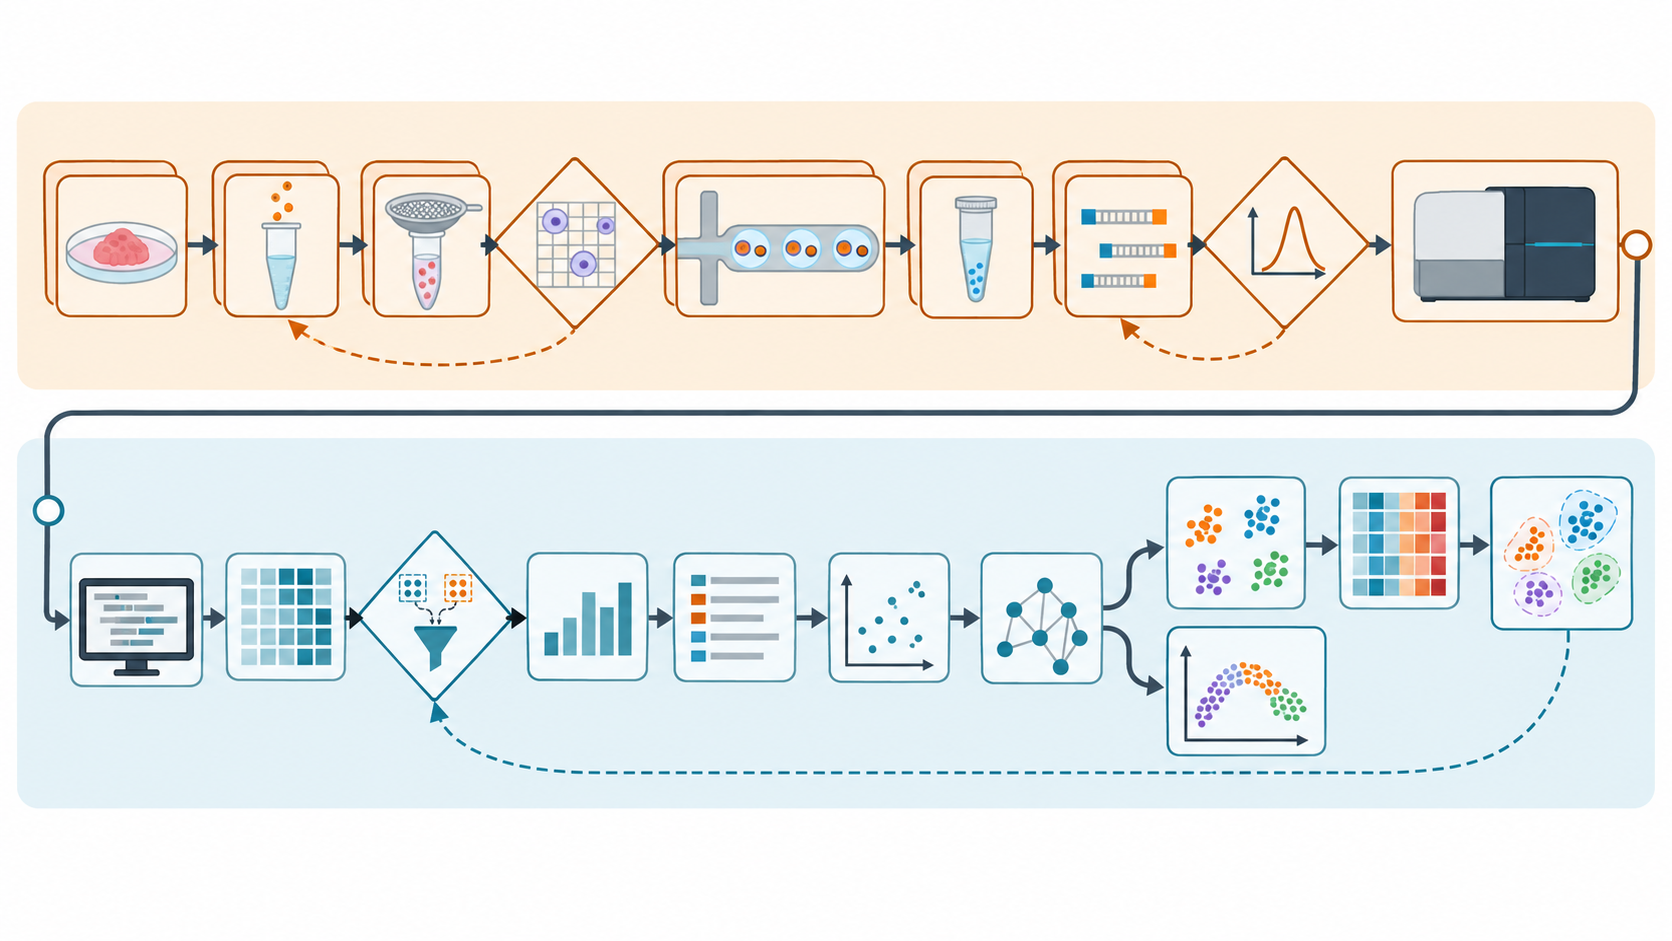
\includegraphics[width=\linewidth]{figures/ch06/ch06-05-v2-brief.png}};
\begin{scope}[x={(img.south east)},y={(img.north west)}]
  \tikzset{
    okmark/.style={draw=white,line width=0.6pt,fill=ChSixGood,text=white,circle,font=\sffamily\bfseries\tiny,inner sep=0.6pt,minimum size=3.6mm},
    ngmark/.style={draw=white,line width=0.6pt,fill=ChSixBad,text=white,circle,font=\sffamily\bfseries\tiny,inner sep=0.6pt,minimum size=3.6mm}
  }
  \node[okmark] at (0.07,0.85) {$\checkmark$};
  \node[okmark] at (0.16,0.85) {$\checkmark$};
  \node[okmark] at (0.25,0.85) {$\checkmark$};
  \node[ngmark] at (0.34,0.86) {$\times$};
  \node[okmark] at (0.25,0.60) {$\checkmark$};
  \node[okmark] at (0.46,0.85) {$\checkmark$};
  \node[okmark] at (0.58,0.85) {$\checkmark$};
  \node[okmark] at (0.67,0.85) {$\checkmark$};
  \node[ngmark] at (0.77,0.86) {$\times$};
  \node[okmark] at (0.72,0.61) {$\checkmark$};
  \node[ngmark] at (0.83,0.77) {$\times$};
  \node[ngmark] at (0.98,0.79) {$\times$};
  \node[okmark] at (0.08,0.44) {$\checkmark$};
  \node[okmark] at (0.17,0.44) {$\checkmark$};
  \node[ngmark] at (0.26,0.47) {$\times$};
  \node[ngmark] at (0.35,0.44) {$\times$};
  \node[okmark] at (0.44,0.44) {$\checkmark$};
  \node[okmark] at (0.53,0.44) {$\checkmark$};
  \node[okmark] at (0.62,0.44) {$\checkmark$};
  \node[okmark] at (0.68,0.42) {$\checkmark$};
  \node[okmark] at (0.68,0.25) {$\checkmark$};
  \node[okmark] at (0.84,0.52) {$\checkmark$};
  \node[ngmark] at (0.93,0.52) {$\times$};
  \node[okmark] at (0.58,0.14) {$\checkmark$};
\end{scope}
\end{tikzpicture}
\caption{A text-free workflow base image generated from the full brief, audited item by item against the step table. Green checkmarks ($\checkmark$) indicate nodes and arrows that match the specification; red crosses ($\times$) mark structural omissions or errors. Although the model preserved the neighbor-graph fork and the three specified feedback arcs, seven structural discrepancies remain across the diamond card stacks, the two sample merge points, the cross-lane hand-off arrow, the optional box placement, and the endpoint tag shapes; consequently, the final figure uses an author-drawn structure with model-generated icons only.}\label{fig:ch06-05}
\end{figure}

Printing Table~\ref{tab:ch06-01} and auditing Figure~\ref{fig:ch06-05} node by node and arrow by arrow shows both the strengths and the limits of full-diagram generation. On the positive side, the model obeyed the ``no text'' constraint, rendered all 20 primary step icons in left-to-right order, split the path after the 7th computational node ($k$-NN network graph) into an upper clustering branch and a lower 2D embedding branch that stops without rejoining, and drew the three specified return arcs (Q1 $\rightarrow$ W2, Q2 $\rightarrow$ W6, and C11 $\rightarrow$ Q3) in the right direction. Nevertheless, the seven red crosses in Figure~\ref{fig:ch06-05} expose structural defects that prevent using the image as a workflow backbone:
\begin{enumerate}
\item \textbf{Incomplete two-sample card stacks (top row, 4th and 8th nodes):} Although the prompt requested two offset cards for steps 1--8, only the six rounded-rectangle steps received double cards; both diamond checkpoints (Q1 and Q2) were drawn as single-layer diamonds.
\item \textbf{Missing sample merge junctions (before the sequencer and at the 4th bottom node):} Only a single arrow connects the library QC diamond to the sequencer, omitting the pooling of two sample libraries; similarly, the normalization node on the bottom row shows no convergence of two filtered matrices.
\item \textbf{Ambiguous cross-lane connector hand-off (top right):} The upper circle connector sits directly against the sequencer border without a distinct hand-off arrow and leaves no space for the ``FASTQ'' product parallelogram.
\item \textbf{Misplaced optional boxes (bottom row, 3rd node):} Instead of placing the two dashed optional boxes (C3a and C3b) above the cell-QC diamond, the model shrank them into tiny dotted squares stuffed \emph{inside} the diamond alongside the filter funnel, leaving no room for text labels.
\item \textbf{Endpoint and icon detail discrepancies (bottom right):} The final cluster map at C11 surrounds the point clusters with dashed outlines rather than blank rounded tag shapes; the PCR tube at step 6 is elongated like a centrifuge tube, and subtle gradients and 3D perspective remain on several vessels.
\end{enumerate}

The V2 experiment demonstrates a clear trade-off: generating a full workflow diagram as a single bitmap can suggest a color palette and icon style, but auditing and fixing its topology takes more effort than drawing a deterministic skeleton—and every regeneration forces you to re-audit all twenty-plus nodes and arrows from scratch.

A cleaner division of labor is the \textbf{icon-sheet workflow (V3)}. Instead of asking the image generator to draw swim lanes and arrows, we generate 12 isolated, style-matched icons on a $4 \times 3$ white grid, slice them into transparent PNGs, and place them onto the deterministic skeleton of Figure~\ref{fig:ch06-03}. In \scidraw{}, an author can enter from the workflow diagram generator (\sdtool{workflow-diagram-generator}) or take the ``Mechanism \& Workflow'' route in the figure workflow wizard (\sdtool{figure-workflow}) into the drawing workspace (\sdtool{ai-drawing}), and submit the 12-icon grid prompt in prompt mode:

\begin{Prompt}
A sheet of twelve flat vector scientific icons arranged in an even grid of four columns
and three rows on a pure white background. Each icon sits centred in its own invisible
square cell with wide white margins and does not touch any other icon. Uniform dark slate
outline of medium weight, flat fills, no gradients, no shadows, no 3D.
Row 1 (warm muted orange-brown accent #B5653A with pale beige fills):
 1. small piece of pink soft tissue on a shallow petri dish;
 2. conical centrifuge tube with three tiny droplets falling into it;
 3. round cell strainer mesh sitting on top of a tube;
 4. square counting grid with five round cells, one cell drawn darker.
Row 2 (same warm accent, except icon 8 in deep amber #8A6D1F):
 5. rectangular microfluidic chip with one channel pinching off round droplets,
    each droplet containing one small cell and one small bead;
 6. single small PCR tube with a closed cap;
 7. three short double-stranded DNA fragments, each with small coloured end caps;
 8. benchtop sequencing instrument: a box with a small slot holding a flow cell.
Row 3 (muted teal-blue accent #2F6F8F with pale blue-grey fills):
 9. computer monitor showing short horizontal bars aligned under one long bar;
10. square grid matrix of small cells with varied light-to-dark shading;
11. network of dots connected by thin edges;
12. four clusters of dots in different muted colours, with blank rounded tag shapes.
No text, no letters, no numbers, no labels, no arrows, no microscope, no DNA helix. 4:3.
\end{Prompt}

Once the $4 \times 3$ icon sheet is generated, each of the 12 cells must be inspected at 200\% zoom for scientific accuracy and visual cleanliness: (1) a small piece of pink soft tissue rests on a shallow Petri dish rather than an intact whole organ; (2) three enzyme droplets fall into a conical centrifuge tube marked only with text-free tick lines; (3) a round cell-strainer mesh sits atop a tube rim; (4) the square counting grid contains five round cells with one shaded darker and no non-cellular debris or numbers; (5) the microfluidic chip shows a single channel pinching off three droplets, each holding one larger nucleated cell and one smaller dark gel bead; (6) a single compact PCR tube has a closed snap cap; (7) three short double-stranded ladder-like DNA fragments carry colored adapter end caps rather than a decorative long double helix; (9) the computer monitor displays short horizontal read bars aligned beneath a long reference bar; (10) the square grid matrix shows light-to-dark expression shading with zero characters; (11) dots and thin edges form a $k$-NN graph without chemical element symbols; and (12) four differently colored point clusters are each paired with a blank rounded tag shape. Across the entire sheet, no letters, numbers, or pseudo-text appear.

Only cell 8 (the benchtop sequencing instrument) failed initial inspection: the model drew an angled front tray holding striped sheets protruding from the housing, making the instrument look like an office desktop printer. Because the icon sheet isolates each graphic in its own grid cell, we do not need to regenerate the other eleven icons. Instead, we select the cropped icon 8 in the \scidraw{} generation history as a reference image and issue a targeted single-icon modification prompt to replace the paper tray with an enclosed optical flow-cell cartridge bay:

\begin{Prompt}
Edit only this one sequencing-instrument icon. Preserve its simple scientific icon style,
dark slate outline, white background, and square framing. Replace the printer-like front
paper tray and paper-output slot with a small closed optical flow-cell cartridge bay:
a glass rectangular microfluidic flow cell in a shallow enclosed cartridge, with tiny
parallel fluidic channels visible through a small window. Use flat pale beige fills with
a restrained deep amber #8A6D1F accent on the cartridge. No sheets of paper, no paper
trays, no keyboards, no text, no letters, no numbers, no labels, no logos. Aspect 1:1.
\end{Prompt}

In the revised icon, the protruding paper tray disappears and is replaced by a recessed deep-amber optical cartridge window on the front panel displaying parallel serpentine microfluidic lanes. Slicing the $4 \times 3$ sheet along equal grid boundaries, converting near-white background pixels to transparency, and padding each bounding box with a uniform 6\% margin yields twelve clean icon assets ready to drop onto the skeleton.

\section{End-to-End Case Study: A Single-Cell RNA-seq Workflow from First Draft to Final Figure}

We now bring together Dr.\ Chen's complete progression from the flawed V1 draft to the verified V4 final figure across three stages.

\textbf{Stage 1: Stepping back from the V1 draft to write the step table and figure brief.}
Instead of endlessly tweaking the one-sentence prompt that produced Figure~\ref{fig:ch06-01}, Dr.\ Chen steps back to her laboratory notebook and analysis scripts, compiles the 20-step source-of-truth table (Table~\ref{tab:ch06-01}), and verifies all nine methodological questions in Table~\ref{tab:ch06-02}. She then opens the \scidraw{} figure workflow wizard (\sdtool{figure-workflow}), selects the ``Mechanism \& Workflow'' route, replaces the default template with her verified figure brief, and saves a local copy:

\begin{Prompt}
[Purpose] Show readers what each step from mouse lung tissue to cell-type annotation does
  and hands off; separate wet lab from computation; show parallel samples, merges, and QC loops.
[Audience & Use] Paper Figure 1A workflow diagram for molecular biologists; full-width 174 mm.
[Required Objects] All 20 primary nodes (W1-W6, Q1, Q2, S1, C1-C11, Q3) and 5 optional nodes
  (W3a, W3b, C3a, C3b, C6a) from Table 6-1, plus key hand-off products: single-cell suspension,
  barcoded cDNA, sequencing library, FASTQ, raw/filtered count matrices, UMAP coords, cell atlas.
[Relations & Arrows] Solid arrow = sequence & hand-off; dashed arc = fail/return; diamond = QC
  gate (pass + fail exits); dashed box = optional; circle A = lane connector; no causal arrows.
[Known, Assumed & Pending] Generic sequence confirmed; all empirical parameters omitted from
  figure ([author to fill in]); batch integration placement simplified and noted in caption.
[Non-negotiable Science] Clustering and UMAP both branch from the k-NN graph (UMAP never links
  to clustering/annotation); libraries pool before sequencing; matrices merge before normalization.
[Layout & Labels] Two horizontal swim lanes read left to right: warm top lane (wet lab & seq.),
  cool bottom lane (computation), joined via connector A (FASTQ). Editable vector labels.
[References] Table 6-1; protocol notes; Luecken & Theis 2019; Zheng et al. 2017.
[Self-Check] Node count, arrows, branches, and merges match Table 6-1; >= 6.5 pt text at print size.
\end{Prompt}

\textbf{Stage 2: Combining the deterministic skeleton with verified AI icons to assemble the V4 final figure.}
After comparing the deterministic skeleton (Figure~\ref{fig:ch06-03}) with the V2 full-diagram generation test (Figure~\ref{fig:ch06-05}), Dr.\ Chen keeps every node coordinate, arrow, branch point, feedback loop, product parallelogram, and vector label from Figure~\ref{fig:ch06-03} unchanged. She places the 12 verified transparent-background icons directly above their corresponding primary nodes (01 $\rightarrow$ W1 Tissue collection; 02 $\rightarrow$ W2 Dissociation; 03 $\rightarrow$ W3 Filtering \& washing; 04 $\rightarrow$ Q1 Count \& viability; 05 $\rightarrow$ W4 Droplet capture \& barcoding; 06 $\rightarrow$ W5 RT \& cDNA amplification; 07 $\rightarrow$ W6 Library construction; 08 $\rightarrow$ S1 Pooling \& sequencing; 09 $\rightarrow$ C1 Alignment \& UMI counting; 10 $\rightarrow$ C2 Cell calling; 11 $\rightarrow$ C7 $k$-NN graph; 12 $\rightarrow$ C11 Cell-type annotation) and leaves the remaining nodes as clean text boxes so the diagram does not become visually overcrowded. The resulting final figure is shown in Figure~\ref{fig:ch06-06}.

\begin{figure}[htbp]\centering
\resizebox{0.94\linewidth}{!}{% FIG ch06-06 final (English)%
\def\ChSixShowIcons{}%
% Shared styles for chapter 6 workflow TikZ figures.%
% Every figure inputs this file, so commands are defined with \providecommand.%
\providecolor{BookTeal}{HTML}{176C68}%
\providecolor{BookInk}{HTML}{23363E}%
\providecolor{BookRule}{HTML}{C8D6D6}%
\providecolor{BookPale}{HTML}{F1F6F5}%
\definecolor{WetPale}{HTML}{FBF1EA}%
\definecolor{Wet}{HTML}{B5653A}%
\definecolor{Seq}{HTML}{8A6D1F}%
\definecolor{DryPale}{HTML}{EEF4F7}%
\definecolor{Dry}{HTML}{2F6F8F}%
\definecolor{ChSixFeedback}{HTML}{7A8A90}%
\definecolor{ChSixBad}{HTML}{C0392B}%
\usetikzlibrary{arrows.meta,positioning,shapes.geometric,shapes.misc,fit,backgrounds,calc}%
\ifdefined\ChSixLayersReady\else%
  \pgfdeclarelayer{chsixlane}%
  \pgfsetlayers{chsixlane,background,main}%
  \def\ChSixLayersReady{}%
\fi%

\tikzset{%
  chsix/.style={font=\sffamily\scriptsize, text=BookInk, align=center},%
  flowstep/.style={%
    chsix, rounded corners=2pt, draw=Wet, line width=0.45pt, fill=white,%
    text width=19mm, minimum height=7.4mm, inner sep=1.3pt,%
  },%
  flowstepdry/.style={flowstep, draw=Dry},%
  flowstepseq/.style={flowstep, draw=Seq},%
  artifact/.style={%
    chsix, trapezium, trapezium left angle=70, trapezium right angle=110,%
    trapezium stretches=true,%
    draw=BookInk, line width=0.45pt, fill=white,%
    minimum height=6.2mm, inner sep=1.2pt,%
  },%
  gate/.style={%
    chsix, diamond, aspect=1.7, draw=BookInk, line width=0.45pt, fill=white,%
    text width=12mm, inner sep=0.6pt, minimum height=8mm,%
  },%
  opt/.style={flowstep, dashed, draw=BookInk!70},%
  optdry/.style={flowstepdry, dashed, draw=BookInk!70},%
  stack/.style={flowstep},%
  link/.style={-{Stealth[length=1.6mm]}, semithick, draw=BookInk},%
  linkthin/.style={-{Stealth[length=1.2mm]}, thin, draw=BookInk!80},%
  back/.style={-{Stealth[length=1.5mm]}, dashed, draw=ChSixFeedback},%
  conn/.style={%
    circle, draw=BookInk, line width=0.5pt, minimum size=4.6mm,%
    font=\sffamily\scriptsize\bfseries, inner sep=0pt, text=BookInk,%
  },%
  lanetitle/.style={font=\sffamily\bfseries\small, text=BookInk, align=left},%
  passlabel/.style={font=\sffamily\scriptsize, text=BookInk, fill=white, inner sep=0.7pt, align=center},%
  mergelabel/.style={font=\sffamily\scriptsize, text=BookInk, fill=white, inner sep=0.8pt, align=center},%
  taglab/.style={font=\sffamily\scriptsize, text=ChSixFeedback, fill=white, inner sep=0.8pt, align=center},%
  gramcap/.style={font=\sffamily\scriptsize, text=BookInk, align=left, anchor=west},%
}%

% Offset card behind a two-sample step. Text stays on the front node only.%
\providecommand{\ChSixCardBack}[1]{%
  \begin{pgfonlayer}{background}%
    \draw[Wet, line width=0.45pt, rounded corners=2pt, fill=white]%
      ([shift={(-0.55mm,0.55mm)}]#1.south west)%
      rectangle ([shift={(-0.55mm,0.55mm)}]#1.north east);%
  \end{pgfonlayer}%
}%
% #1 options, #2 name, #3 position (with parentheses), #4 text%
\providecommand{\ChSixCard}[4]{%
  \node[stack, #1] (#2) at #3 {#4};%
  \ChSixCardBack{#2}%
}%

\providecommand{\ChSixMaybeLabel}[1]{%
  \ifdefined\nolabels\else#1\fi%
}%

\providecommand{\ChSixIcon}[2]{%
  \ifdefined\ChSixShowIcons%
    \IfFileExists{#1}{%
      \node[anchor=south, inner sep=0] at ([yshift=0.7mm]#2.north)%
        {\includegraphics[height=5.4mm]{#1}};%
    }{}%
  \fi%
}%
%
% English node labels for FIG ch06-03 / ch06-06%
\providecommand{\ChSixLaneWet}{Wet lab \& sequencing}%
\providecommand{\ChSixLaneDry}{Computational analysis}%
\providecommand{\ChSixTxtWone}{Tissue\\collection}%
\providecommand{\ChSixTxtWtwo}{Dissociation}%
\providecommand{\ChSixTxtWthree}{Filtering\\\& washing}%
\providecommand{\ChSixTxtWthreeA}{RBC lysis}%
\providecommand{\ChSixTxtWthreeB}{Dead-cell\\removal}%
\providecommand{\ChSixTxtQone}{Count \&\\viability}%
\providecommand{\ChSixTxtWfour}{Droplet capture\\\& barcoding}%
\providecommand{\ChSixTxtWfive}{RT \& cDNA\\amplification}%
\providecommand{\ChSixTxtWsix}{Library\\construction}%
\providecommand{\ChSixTxtQtwo}{Library\\QC}%
\providecommand{\ChSixTxtSone}{Pooling \&\\sequencing}%
\providecommand{\ChSixTxtCone}{Alignment \&\\UMI counting}%
\providecommand{\ChSixTxtCtwo}{Cell calling}%
\providecommand{\ChSixTxtQthree}{Cell QC}%
\providecommand{\ChSixTxtCthreeA}{Doublet\\detection}%
\providecommand{\ChSixTxtCthreeB}{Ambient RNA\\correction}%
\providecommand{\ChSixTxtCfour}{Merge \&\\normalize}%
\providecommand{\ChSixTxtCfive}{Highly\\variable genes}%
\providecommand{\ChSixTxtCsix}{PCA}%
\providecommand{\ChSixTxtCsixA}{Integration\\(optional)}%
\providecommand{\ChSixTxtCseven}{k-NN graph}%
\providecommand{\ChSixTxtCeight}{Clustering\\(Leiden)}%
\providecommand{\ChSixTxtCnine}{UMAP}%
\providecommand{\ChSixTxtCten}{Marker\\genes}%
\providecommand{\ChSixTxtCeleven}{Cell-type\\annotation}%
\providecommand{\ChSixArtSusp}{Single-cell\\suspension}%
\providecommand{\ChSixArtCdna}{Barcoded\\cDNA}%
\providecommand{\ChSixArtLib}{Sequencing\\library}%
\providecommand{\ChSixArtFastq}{FASTQ}%
\providecommand{\ChSixArtRaw}{Raw count\\matrix}%
\providecommand{\ChSixArtFilt}{Filtered\\matrix}%
\providecommand{\ChSixArtAtlas}{Annotated\\cell atlas}%
\providecommand{\ChSixArtUmap}{UMAP coordinates\\(display only)}%
\providecommand{\ChSixQoneFail}{Fail: optimise\\dissociation}%
\providecommand{\ChSixQtwoFail}{Fail}%
\providecommand{\ChSixCelevenFail}{Low-quality clusters\\or poor resolution}%
\providecommand{\ChSixMergeNote}{Two samples merge here}%
\providecommand{\ChSixPass}{Pass}%
%
\begin{tikzpicture}[x=1cm,y=1cm]%
  % Row positions are set with relative anchors in ch06-workflow-draw.tex%
% so Chinese and English labels do not share one set of fixed centres.%
%
  % Workflow structure (FIG ch06-03 skeleton / ch06-06 final).%
% Requires ch06-styles and a label file. Nodes are placed from the node%
% above them so wrapped English labels cannot land on the next row.%
\coordinate (origin) at (0,0);%
% Final figures carry icons above the nodes; keep feedback arcs above them.%
\ifdefined\ChSixShowIcons
  \def\ChSixLift{6.6mm}%
  \def\ChSixArc{12.2mm}%
\else
  \def\ChSixLift{0mm}%
  \def\ChSixArc{8.4mm}%
\fi

% ----- Wet lab, row 1: collection through droplet capture -----%
\ChSixCard{anchor=north west}{nW1}{(origin)}{\ChSixMaybeLabel{\ChSixTxtWone}}%
\ChSixCard{anchor=west}{nW2}{([xshift=3.2mm]nW1.east)}{\ChSixMaybeLabel{\ChSixTxtWtwo}}%
\ChSixCard{anchor=west}{nW3}{([xshift=3.2mm]nW2.east)}{\ChSixMaybeLabel{\ChSixTxtWthree}}%
\node[gate, anchor=west] (nQ1) at ([xshift=3.6mm]nW3.east) {\ChSixMaybeLabel{\ChSixTxtQone}};%
\ChSixCard{anchor=west}{nW4}{([xshift=6.4mm]nQ1.east)}{\ChSixMaybeLabel{\ChSixTxtWfour}}%

\draw[link] (nW1) -- (nW2);%
\draw[link] (nW2) -- (nW3);%
\draw[link] (nW3) -- (nQ1);%
\draw[link] (nQ1) -- (nW4);%

\coordinate (arcQ1) at ($(nW2.north)!0.5!(nQ1.north)+(0,\ChSixArc)$);%
\draw[back] ([yshift=\ChSixLift]nQ1.north) -- ([yshift=\ChSixLift]nQ1.north |- arcQ1) -- ([yshift=\ChSixLift]nW2.north |- arcQ1) -- ([yshift=\ChSixLift]nW2.north);%
\node[taglab, anchor=south] (q1fail) at (arcQ1) {\ChSixMaybeLabel{\ChSixQoneFail}};%
\node[passlabel] (passQ1) at ($(nQ1.east)!0.5!(nW4.west)+(0,1.3mm)$) {\ChSixMaybeLabel{\ChSixPass}};%

\node[lanetitle, anchor=south west] (laneWet) at ([yshift=1.2mm]q1fail.north -| origin) {\ChSixMaybeLabel{\ChSixLaneWet}};%

% Optional lysis / dead-cell removal under filtering, product to their right.%
\node[opt, anchor=north] (nW3a) at ([yshift=-2.2mm]nW3.south) {\ChSixMaybeLabel{\ChSixTxtWthreeA}};%
\node[opt, anchor=north] (nW3b) at ([yshift=-1.8mm]nW3a.south) {\ChSixMaybeLabel{\ChSixTxtWthreeB}};%
\draw[linkthin] (nW3.south) -- (nW3a.north);%
\draw[linkthin] (nW3a.south) -- (nW3b.north);%
\node[artifact, anchor=north west] (aSusp) at ([xshift=3.2mm, yshift=-2.2mm]nW3.south east) {\ChSixMaybeLabel{\ChSixArtSusp}};%

% ----- Wet lab, row 2 (left-aligned; FASTQ is the hand-off into connector A) -----%
\ChSixCard{anchor=north west}{nW5}{([yshift=-10mm]nW3b.south -| nW1.west)}{\ChSixMaybeLabel{\ChSixTxtWfive}}%
\ChSixCard{anchor=west}{nW6}{([xshift=2.4mm]nW5.east)}{\ChSixMaybeLabel{\ChSixTxtWsix}}%
\node[gate, anchor=west] (nQ2) at ([xshift=2.4mm]nW6.east) {\ChSixMaybeLabel{\ChSixTxtQtwo}};%
\node[flowstepseq, anchor=west] (nS1) at ([xshift=6.2mm]nQ2.east) {\ChSixMaybeLabel{\ChSixTxtSone}};%
\node[artifact, anchor=west] (aFastq) at ([xshift=2.2mm]nS1.east) {\ChSixMaybeLabel{\ChSixArtFastq}};%
\node[conn, anchor=west] (nA) at ([xshift=2mm]aFastq.east) {A};%

\draw[link] (nW5) -- (nW6);%
\draw[link] (nW6) -- (nQ2);%
\draw[link] (nQ2) -- (nS1);%
\draw[link] (nS1) -- (aFastq);%
\draw[link] (aFastq) -- (nA);%
\node[passlabel] (passQ2) at ($(nQ2.east)!0.5!(nS1.west)+(0,1.3mm)$) {\ChSixMaybeLabel{\ChSixPass}};%

\coordinate (arcQ2) at ($(nW6.north)!0.5!(nQ2.north)+(0,\ChSixArc)$);%
\draw[back] ([yshift=\ChSixLift]nQ2.north) -- ([yshift=\ChSixLift]nQ2.north |- arcQ2) -- ([yshift=\ChSixLift]nW6.north |- arcQ2) -- ([yshift=\ChSixLift]nW6.north);%
\node[taglab, anchor=south] (q2fail) at (arcQ2) {\ChSixMaybeLabel{\ChSixQtwoFail}};%

\node[artifact, anchor=north] (aCdna) at ([yshift=-2mm]$(nW5.south)!0.5!(nW6.south)$) {\ChSixMaybeLabel{\ChSixArtCdna}};%
\node[artifact, anchor=north] (aLib) at ([yshift=-2mm]$(nW6.south)!0.5!(nQ2.south)$) {\ChSixMaybeLabel{\ChSixArtLib}};%

% ----- Computational lane -----%
\node[conn, anchor=north west] (nA2) at ([yshift=-7mm]aCdna.south -| origin) {A};%
\node[flowstepdry, anchor=west] (nC1) at ([xshift=3.2mm]nA2.east) {\ChSixMaybeLabel{\ChSixTxtCone}};%
\node[flowstepdry, anchor=west] (nC2) at ([xshift=3.6mm]nC1.east) {\ChSixMaybeLabel{\ChSixTxtCtwo}};%
\node[gate, anchor=west] (nQ3) at ([xshift=4.2mm]nC2.east) {\ChSixMaybeLabel{\ChSixTxtQthree}};%
\node[flowstepdry, anchor=west] (nC4) at ([xshift=4.2mm]nQ3.east) {\ChSixMaybeLabel{\ChSixTxtCfour}};%
\node[flowstepdry, anchor=west] (nC5) at ([xshift=3.6mm]nC4.east) {\ChSixMaybeLabel{\ChSixTxtCfive}};%

\draw[link] (nA2) -- (nC1);%
\draw[link] (nC1) -- (nC2);%
\draw[link] (nC2) -- (nQ3);%
\draw[link] (nQ3) -- (nC4);%
\draw[link] (nC4) -- (nC5);%

\node[mergelabel, anchor=south] (mergeNote) at ([yshift=1mm]nC4.north) {\ChSixMaybeLabel{\ChSixMergeNote}};%

\coordinate (arcDry) at ($(nC1.north)!0.5!(nQ3.north)+(0,\ChSixArc)$);%
\node[taglab, anchor=south, text width=28mm] (c11fail) at (arcDry) {\ChSixMaybeLabel{\ChSixCelevenFail}};%
\node[lanetitle, anchor=south west] (laneDry) at ([yshift=1.2mm]c11fail.north -| origin) {\ChSixMaybeLabel{\ChSixLaneDry}};%

% Optional doublet / ambient RNA under the cell-QC gate.%
\node[optdry, anchor=north east] (nC3a) at ([yshift=-2mm, xshift=-1mm]nQ3.south) {\ChSixMaybeLabel{\ChSixTxtCthreeA}};%
\node[optdry, anchor=north west] (nC3b) at ([yshift=-2mm, xshift=1mm]nQ3.south) {\ChSixMaybeLabel{\ChSixTxtCthreeB}};%
\draw[linkthin] (nQ3.south) -- (nC3a.north);%
\draw[linkthin] (nQ3.south) -- (nC3b.north);%
\draw[linkthin] (nC3a.south) -- ++(0,-2.4mm) -| (nC3b.south);%

\node[artifact, anchor=north] (aRaw) at ([yshift=-2mm]$(nC1.south)!0.5!(nC2.south)$) {\ChSixMaybeLabel{\ChSixArtRaw}};%
\node[artifact, anchor=north] (aFilt) at ([yshift=-2mm]nC4.south) {\ChSixMaybeLabel{\ChSixArtFilt}};%

% Fork: k-NN graph splits to clustering (continues) and UMAP (display only).%
\node[flowstepdry, anchor=north west] (nC6) at ([yshift=-4mm]aRaw.south -| nC1.west) {\ChSixMaybeLabel{\ChSixTxtCsix}};%
\node[flowstepdry, anchor=west] (nC7) at ([xshift=4mm]nC6.east) {\ChSixMaybeLabel{\ChSixTxtCseven}};%
\node[flowstepdry, anchor=west] (nC8) at ([xshift=5mm]nC7.east) {\ChSixMaybeLabel{\ChSixTxtCeight}};%
\node[flowstepdry, anchor=west] (nC10) at ([xshift=3.6mm]nC8.east) {\ChSixMaybeLabel{\ChSixTxtCten}};%
\node[flowstepdry, anchor=west] (nC11) at ([xshift=3.6mm]nC10.east) {\ChSixMaybeLabel{\ChSixTxtCeleven}};%
\node[optdry, anchor=north] (nC6a) at ([yshift=-2mm]nC6.south) {\ChSixMaybeLabel{\ChSixTxtCsixA}};%
\node[flowstepdry, anchor=north] (nC9) at ([yshift=-3.2mm]nC7.south) {\ChSixMaybeLabel{\ChSixTxtCnine}};%
\node[artifact, anchor=north, text width=22mm] (aUmap) at ([yshift=-1.8mm]nC9.south) {\ChSixMaybeLabel{\ChSixArtUmap}};%
\node[artifact, anchor=north] (aAtlas) at ([yshift=-2mm]$(nC10.south)!0.5!(nC11.south)$) {\ChSixMaybeLabel{\ChSixArtAtlas}};%

\draw[link] (nC5.south) -- ++(0,-2.5mm) -| (nC6.north);%
\draw[linkthin] (nC6.south) -- (nC6a.north);%
\draw[link] (nC6) -- (nC7);%
\draw[link] (nC7) -- (nC8);%
\draw[link] (nC8) -- (nC10);%
\draw[link] (nC10) -- (nC11);%
\draw[link] (nC7.south) -- (nC9.north);%

% Return from annotation to clustering, and the long return to cell QC.%
\coordinate (bus) at ([yshift=-4.5mm]aUmap.south);%
\draw[back] (nC11.south) -- (nC11.south |- bus) -- (nC8.south |- bus) -- (nC8.south);%
\draw[back] (nC11.east) -- ++(3.2mm,0) |- (c11fail.east);%
\draw[back] (c11fail.west) -| ([yshift=\ChSixLift]nQ3.north);%

% Connector A joins the lanes in the gutter between them.%
\draw[link] (nA.south) -- ++(0,-2.2mm) -| (nA2.north);%

\ChSixIcon{figures/ch06/icons/ch06-icon-01.png}{nW1}%
\ChSixIcon{figures/ch06/icons/ch06-icon-02.png}{nW2}%
\ChSixIcon{figures/ch06/icons/ch06-icon-03.png}{nW3}%
\ChSixIcon{figures/ch06/icons/ch06-icon-04.png}{nQ1}%
\ChSixIcon{figures/ch06/icons/ch06-icon-05.png}{nW4}%
\ChSixIcon{figures/ch06/icons/ch06-icon-06.png}{nW5}%
\ChSixIcon{figures/ch06/icons/ch06-icon-07.png}{nW6}%
\ChSixIcon{figures/ch06/icons/ch06-icon-08.png}{nS1}%
\ChSixIcon{figures/ch06/icons/ch06-icon-09.png}{nC1}%
\ChSixIcon{figures/ch06/icons/ch06-icon-10.png}{nC2}%
\ChSixIcon{figures/ch06/icons/ch06-icon-11.png}{nC7}%
\ChSixIcon{figures/ch06/icons/ch06-icon-12.png}{nC11}%

\begin{pgfonlayer}{chsixlane}%
  \node[rectangle, fit=(laneWet)(nW1)(nW4)(nW3b)(aSusp)(nA)(aCdna)(aLib)(q1fail),%
        fill=WetPale, draw=none, inner sep=1.1mm] {};%
  \node[rectangle, fit=(laneDry)(nA2)(nC5)(nC11)(nC6a)(aUmap)(aAtlas)(c11fail)(nC3a)(nC3b),%
        fill=DryPale, draw=none, inner sep=1.1mm] {};%
\end{pgfonlayer}%
%
\end{tikzpicture}%
}
\caption{Experimental and computational workflow for droplet-based single-cell RNA sequencing (schematic). Top, wet-lab and sequencing steps (warm lane): control and treated samples are dissociated, captured, and converted to libraries separately (stacked boxes) and pooled for sequencing. Bottom, computational analysis (cool lane), continued from FASTQ files via connector A. Diamonds are quality-control gates; dashed arcs return to an earlier step when a gate fails or results are anomalous; dashed boxes are optional steps. Clustering and UMAP are both computed from the $k$-nearest-neighbor graph in principal-component space; UMAP is used for display only. The diagram simplifies a generic protocol and omits parameters, single-nucleus protocols, sample multiplexing, trajectory, and differential-abundance analyses; where integration sits varies between software packages. Icons were made with an image-generation model and checked by hand; the workflow structure and all text were drawn by the authors.}\label{fig:ch06-06}
\end{figure}

\textbf{Stage 3: Drafting the figure legend and completing the item-by-item final verification log.}
Starting from a draft description generated by the \scidraw{} figure legend assistant (\sdtool{figure-legend}), Dr.\ Chen adds explicit statements covering the scope of protocol simplification, software-specific variations in integration placement, and the division of labor between AI icon generation and author-drawn structure:

\begin{BookNote}
\textbf{Figure 6-6 | Experimental and computational workflow for droplet-based single-cell RNA sequencing (schematic).} Top, wet-lab and sequencing steps (warm lane): control and treated samples are dissociated, captured, and converted to libraries separately (stacked boxes) and pooled for sequencing. Bottom, computational analysis (cool lane), continued from FASTQ files via connector A. Diamonds are quality-control gates; dashed arcs return to an earlier step when a gate fails or results are anomalous; dashed boxes are optional steps. Clustering and UMAP are both computed from the $k$-nearest-neighbor graph in principal-component space; UMAP is used for display only. The diagram simplifies a generic protocol and omits parameters, single-nucleus protocols, sample multiplexing, trajectory, and differential-abundance analyses; where integration sits varies between software packages. Icons were made with an image-generation model and checked by hand; the workflow structure and all text were drawn by the authors.
\end{BookNote}

Before packaging the figure for submission, Dr.\ Chen runs the \scidraw{} figure checker (\sdtool{figure-checker}) to inspect print dimensions, grayscale contrast, and color-vision accessibility, and then completes the line-by-line verification log against Table~\ref{tab:ch06-01} (Table~\ref{tab:ch06-04}).

\begin{table}[htbp]\centering\footnotesize
\setlength{\tabcolsep}{4pt}
\renewcommand{\arraystretch}{1.12}
\caption{Item-by-item final verification log for the single-cell RNA-seq workflow diagram (Figure~\ref{fig:ch06-06}).}\label{tab:ch06-04}
\begin{tabularx}{\linewidth}{@{}>{\raggedright\arraybackslash}p{24mm}YY@{}}
\toprule
\textbf{Check item} & \textbf{Brief \& step-table expectation} & \textbf{Figure~\ref{fig:ch06-06} final verification result} \\
\midrule
Node count & 20 primary nodes (9 wet-lab/sequencing: W1--W6, Q1, Q2, S1; 11 computational: C1--C11, Q3) + 5 optional nodes (W3a, W3b, C3a, C3b, C6a) + 8 product nodes & All present and structurally identical to the Figure~\ref{fig:ch06-03} skeleton \\
Sequence arrows & Every solid arrow matches the ``Next'' column of Table~\ref{tab:ch06-01} one-to-one & Verified arrow by arrow; cross-lane continuation linked cleanly via connector A \\
Branching topology & C7 $\rightarrow$ C8 (Leiden clustering) and C7 $\rightarrow$ C9 (UMAP); parallel C3a $\parallel$ C3b under Q3 & Fork junction and parallel optional branches connected accurately \\
Sample merges & S1 (two sample libraries pooled); C4 (two filtered count matrices merged) & Offset double cards on W1--W6 converge to single box at S1; merge explicitly labeled above C4 \\
Feedback arcs & Q1 $\rightarrow$ W2; Q2 $\rightarrow$ W6; C11 $\rightarrow$ Q3; C11 $\rightarrow$ C8 & All four dashed return arcs match expected line style, direction, and condition labels \\
QC gate exits & Q1, Q2, and Q3 each have a forward pass path and an anomaly/failure return path & Diamond nodes carry complete dual-exit routing \\
Prohibited links & C9 never connects to C8 or C11; no causal arrows; no unverified parameter values & Confirmed zero prohibited connections and zero parameter numbers \\
Icons \& text & 12 icons matched to primary steps, zero text at 200\% zoom; editable vector labels $\ge 6.5\text{ pt}$ at final print width & All 12 icons positioned accurately with no pseudo-text (sequencer icon requires confirming replacement with the flow-cell cartridge version); font size legible \\
\bottomrule
\end{tabularx}
\end{table}

\section{What AI Can and Cannot Do in This Step}

Table~\ref{tab:ch06-03} summarizes the division of responsibility between AI tools and the author at each stage of creating a method or workflow diagram.

\begin{table}[htbp]\centering\footnotesize
\setlength{\tabcolsep}{3pt}
\renewcommand{\arraystretch}{1.12}
\caption{What AI can do, what it cannot do, and what the author must verify when making method and workflow diagrams.}\label{tab:ch06-03}
\begin{tabularx}{\linewidth}{@{}>{\raggedright\arraybackslash}p{20mm}YYY@{}}
\toprule
\textbf{Stage} & \textbf{What AI can do} & \textbf{What AI cannot do / should not be given} & \textbf{What the author must verify} \\
\midrule
Organizing methods & Extract candidate steps from prose notes and flag missing products, QC gates, or branches & Know which optional steps you actually ran; supply real parameters (it will invent plausible-sounding numbers) & Every row of the step table matches lab records; all parameters come from records, with AI suggestions marked pending confirmation \\
Structure & Generate a full image that ``looks like a flowchart''; use sketch mode to reference an uploaded skeleton layout & Guarantee exact node counts, arrow directions, branches, or merge points; a sketch is not a structural lock & Audit every node and arrow item by item against the step table \\
Icons \& style & Generate a style-consistent icon sheet; edit a single icon by instruction; continue editing from history & Guarantee that an icon is scientifically accurate (e.g., one cell per droplet) or spell technical terms in bitmaps & Scientific meaning of each icon; zero text or pseudo-text in the base images \\
Labels & — (all final text in this chapter is rendered deterministically in TikZ) & Reliably spell long technical terms inside an image-generation model & Terminology, abbreviations, and software names are accurate and consistent \\
Figure legend & Draft an initial description from the figure using \sdtool{figure-legend} & Know what was simplified, what was omitted, or which parameters remain pending & State the scope of simplification, optional steps, icon source, and AI role \\
Technical check & Inspect dimensions, resolution, grayscale contrast, and color-vision risk via \sdtool{figure-checker} & Judge whether the workflow topology is scientifically valid & Domain peer review of the experimental and analytical sequence \\
\bottomrule
\end{tabularx}
\end{table}

\section{Chapter Checklist}

\begin{itemize}
\item A structured step table exists: every box in the diagram maps to a row in the table, and every row in the table either appears in the diagram or is explicitly declared as omitted in the caption.
\item Operational steps (what is done) and products (what material or data is handed off) use distinct shapes, with product nodes placed at key hand-offs.
\item Every quality-control or decision gate has both a ``Pass'' and a ``Fail'' exit whose routing matches actual laboratory or analytical practice.
\item Parallel sample processing is drawn in parallel (or as offset stacked cards) with explicit merge points; optional steps use a uniform dashed border, and unperformed optional steps have been deleted.
\item Feedback and iterative return loops use a line style visually distinct from forward sequence arrows.
\item Wet-lab and computational stages (or other major phases) are immediately distinguishable by both swim-lane background fills and bold text headers.
\item Workflow arrows represent sequence and hand-off only; mechanistic effects or biological caveats are written as annotations or in the figure caption.
\item Visualization embeddings (such as UMAP) are never drawn upstream of analytical steps (such as graph clustering).
\item No unconfirmed parameters appear in the diagram, base images contain zero pseudo-text, and all text labels remain editable.
\item The figure caption states the scope of protocol simplification and how the icons were generated (the example images in this chapter were generated with an image model; prompts and generation records are available in the book repository).
\end{itemize}

\section{Exercises}

\begin{enumerate}
\item \textbf{From prose protocol to step table:} Select a paragraph from the Methods section of one of your own manuscripts (or use the first paragraph of the pedagogical protocol in Section 6.2). Decompose it into a structured step table (ID, Step, Lane, Input, Product, Key conditions, QC / decision, and Next), and list at least five empirical parameters or procedural questions that require author confirmation against raw laboratory records.
\item \textbf{Hands-on practice with \scidraw{}:} Open the figure workflow wizard (\sdtool{figure-workflow}), choose the ``Mechanism \& Workflow'' route, and enter the drawing workspace (\sdtool{ai-drawing}). First, generate a workflow diagram for your protocol from a single sentence and save it as V1. Next, write a text-free icon-sheet prompt (6--12 isolated icons on a grid) to generate style-matched icons, and use reference-image editing from your generation history to revise one icon that fails scientific inspection. Finally, draw the structural skeleton from your step table in PowerPoint, draw.io, or TikZ and place the verified icons onto the skeleton. Submit your V1 image, icon sheet, single-icon revision prompt, final diagram, and item-by-item verification table.
\item \textbf{Cross-disciplinary structural debugging (computer \& data science):} A colleague drafts a machine-learning workflow diagram chained as follows: ``Raw dataset $\rightarrow$ Feature standardization (compute mean and variance across all samples) $\rightarrow$ Train/test split $\rightarrow$ Model training $\rightarrow$ Evaluation on test set.'' Identify the data-leakage error in this topology (standardization parameters must be fit exclusively on the training split and then applied to transform the test split), redraw the diagram using the node and arrow grammar of this chapter (``Raw dataset'' $\rightarrow$ ``Train/test split'' $\rightarrow$ parallel ``Training set'' and ``Test set'' products $\rightarrow$ fit scaler on training set $\rightarrow$ apply fitted parameters to transform both training and test sets in parallel $\rightarrow$ ``Model training'' $\rightarrow$ ``Evaluation on test set''), and write a one-sentence caption explaining why the branch topology prevents test-set leakage.
\end{enumerate}

\section*{References}

\begin{itemize}\sloppy
\item Heumos L, Schaar AC, Lance C, Litinetskaya A, Drost F, Zappia L, Lücken MD, Strobl DC, Henao J, Curion F, Single-cell Best Practices Consortium, Schiller HB, Theis FJ. Best practices for single-cell analysis across modalities. \textit{Nature Reviews Genetics}. 2023;24:550--572. doi:10.1038/s41576-023-00586-w
\item Hwang B, Lee JH, Bang D. Single-cell RNA sequencing technologies and bioinformatics pipelines. \textit{Experimental \& Molecular Medicine}. 2018;50:96. doi:10.1038/s12276-018-0071-8
\item Islam S, Zeisel A, Joost S, La Manno G, Zajac P, Kasper M, Lönnerberg P, Linnarsson S. Quantitative single-cell RNA-seq with unique molecular identifiers. \textit{Nature Methods}. 2014;11(2):163--166. doi:10.1038/nmeth.2772
\item Luecken MD, Theis FJ. Current best practices in single-cell RNA-seq analysis: a tutorial. \textit{Molecular Systems Biology}. 2019;15(6):e8746. doi:10.15252/msb.20188746
\item Macosko EZ, Basu A, Satija R, Nemesh J, Shekhar K, Goldman M, Tirosh I, Bialas AR, Kamitaki N, Martersteck EM, Trombetta JJ, Weitz DA, Sanes JR, Shalek AK, Regev A, McCarroll SA. Highly parallel genome-wide expression profiling of individual cells using nanoliter droplets. \textit{Cell}. 2015;161(5):1202--1214. doi:10.1016/j.cell.2015.05.002
\item Traag VA, Waltman L, van Eck NJ. From Louvain to Leiden: guaranteeing well-connected communities. \textit{Scientific Reports}. 2019;9:5233. doi:10.1038/s41598-019-41695-z
\item van den Brink SC, Sage F, Vértesy Á, Spanjaard B, Peterson-Maduro J, Baron CS, Robin C, van Oudenaarden A. Single-cell sequencing reveals dissociation-induced gene expression in tissue subpopulations. \textit{Nature Methods}. 2017;14:935--936. doi:10.1038/nmeth.4437
\item Wolf FA, Angerer P, Theis FJ. SCANPY: large-scale single-cell gene expression data analysis. \textit{Genome Biology}. 2018;19:15. doi:10.1186/s13059-017-1382-0
\item Wolock SL, Lopez R, Klein AM. Scrublet: computational identification of cell doublets in single-cell transcriptomic data. \textit{Cell Systems}. 2019;8(4):281--291.e9. doi:10.1016/j.cels.2018.11.005
\item Wong B. Points of view: Gestalt principles (Part 2). \textit{Nature Methods}. 2010;7:941. doi:10.1038/nmeth1210-941
\item Wong B. Points of view: simplify to clarify. \textit{Nature Methods}. 2011a;8:611. doi:10.1038/nmeth.1660
\item Wong B. Points of view: arrows. \textit{Nature Methods}. 2011b;8:701. doi:10.1038/nmeth.1676
\item Young MD, Behjati S. SoupX removes ambient RNA contamination from droplet-based single-cell RNA sequencing data. \textit{GigaScience}. 2020;9(12):giaa151. doi:10.1093/gigascience/giaa151
\item Zheng GXY, Terry JM, Belgrader P, Ryvkin P, Bent ZW, Wilson R, Ziraldo SB, Wheeler TD, McDermott GP, Zhu J, Gregory MT, Shuga J, Montesclaros L, Underwood JG, Masquelier DA, Nishimura SY, Schnall-Levin M, Wyatt PW, Hindson CM, Bharadwaj R, Wong A, Ness KD, Beppu LW, Deeg HJ, McFarland C, Loeb KR, Valente WJ, Ericson NG, Stevens EA, Radich JP, Mikkelsen TS, Hindson BJ, Bielas JH. Massively parallel digital transcriptional profiling of single cells. \textit{Nature Communications}. 2017;8:14049. doi:10.1038/ncomms14049
\end{itemize}

% TODO: figures/ch06/ch06-05-v2-scidraw.png (SciDraw AI screenshot for optional panel B of FIG ch06-05, not present on disk)
% TODO: figures/ch06/ch06-workflow-draw.tex line 127 references figures/ch06/icons/ch06-icon-08.png instead of figures/ch06/icons/ch06-icon-08-corrected.png

\chapter{Mechanism and Structure Schematics}

\makeatletter
\@ifundefined{chsevenrelmark}{%
\newcommand{\chsevenrelmark}[2][]{%
  \tikz[baseline=(char.base)]{%
    \node[shape=circle, draw=BookInk, line width=0.5pt, fill=white, inner sep=1pt,
      font=\sffamily\fontsize{6.5}{6.5}\selectfont, #1] (char)
      {\@ifundefined{chseven@num@#2}{#2}{\csname chseven@num@#2\endcsname}};}}%
}{}
\definecolor{ch07err}{HTML}{C0392B}
\@ifundefined{chsevenerrmark}{%
\newcommand{\chsevenerrmark}[2][]{%
  \tikz[baseline=(char.base)]{%
    \node[shape=circle, fill=ch07err, text=white, inner sep=1.5pt,
      font=\sffamily\fontsize{7}{7}\selectfont\bfseries, #1] (char)
      {\@ifundefined{chseven@num@#2}{#2}{\csname chseven@num@#2\endcsname}};}}%
}{}
\@ifundefined{chsevenpanelbase}{%
  \newcommand{\chsevenpanelbase}{figures/ch07/ch07-08-battery-base.png}%
}{}
\@ifundefined{chsevendrawcircuit}{%
\newcommand{\chsevendrawcircuit}[1]{%
  \def\ChSevenWireY{1.10}%
  \def\ChSevenTabY{0.878}%
  \draw[ch07wire, line width=0.8pt] (0.194, \ChSevenTabY) -- (0.194, \ChSevenWireY);
  \draw[ch07wire, line width=0.8pt] (0.805, \ChSevenTabY) -- (0.805, \ChSevenWireY);
  \draw[ch07wire, line width=0.8pt] (0.194, \ChSevenWireY) -- (0.805, \ChSevenWireY);
  \node[draw=ch07wire, line width=0.6pt, rounded corners=1.5pt, fill=white,
    font=\sffamily\scriptsize, inner sep=1.6pt]
    at (0.50, \ChSevenWireY) {#1};
  \foreach \chyy in {0.38, 0.52, 0.66} {%
    \draw[-{Stealth[length=2mm]}, ch07Li, line width=0.9pt]
      (0.68, 1-\chyy) -- (0.32, 1-\chyy);
  }%
  \node[font=\sffamily\scriptsize, text=ch07Li, fill=white, inner sep=0.7pt]
    at (0.50, 1-0.30) {Li\textsuperscript{+}};
  \draw[ch07elec, line width=0.7pt, dashed, -{Stealth[length=1.5mm]}]
    (0.76, \ChSevenWireY) -- (0.62, \ChSevenWireY);
  \draw[ch07elec, line width=0.7pt, dashed, -{Stealth[length=1.5mm]}]
    (0.38, \ChSevenWireY) -- (0.24, \ChSevenWireY);
}%
}{}
\@ifundefined{chsevendrawcircuitb}{%
\newcommand{\chsevendrawcircuitb}[1]{%
  \def\ChSevenWireY{1.10}%
  \def\ChSevenTabY{0.878}%
  \draw[ch07wire, line width=0.8pt] (0.194, \ChSevenTabY) -- (0.194, \ChSevenWireY);
  \draw[ch07wire, line width=0.8pt] (0.805, \ChSevenTabY) -- (0.805, \ChSevenWireY);
  \draw[ch07wire, line width=0.8pt] (0.194, \ChSevenWireY) -- (0.805, \ChSevenWireY);
  \node[draw=ch07wire, line width=0.6pt, rounded corners=1.5pt, fill=white,
    font=\sffamily\scriptsize, inner sep=1.6pt]
    at (0.50, \ChSevenWireY) {#1};
  \foreach \chyy in {0.38, 0.52, 0.66} {%
    \draw[-{Stealth[length=2mm]}, ch07Li, line width=0.9pt]
      (0.32, 1-\chyy) -- (0.68, 1-\chyy);
  }%
  \node[font=\sffamily\scriptsize, text=ch07Li, fill=white, inner sep=0.7pt]
    at (0.50, 1-0.30) {Li\textsuperscript{+}};
  \draw[ch07elec, line width=0.7pt, dashed, -{Stealth[length=1.5mm]}]
    (0.24, \ChSevenWireY) -- (0.38, \ChSevenWireY);
  \draw[ch07elec, line width=0.7pt, dashed, -{Stealth[length=1.5mm]}]
    (0.62, \ChSevenWireY) -- (0.76, \ChSevenWireY);
}%
}{}
\makeatother

While drafting a manuscript on insulin resistance in skeletal muscle, a graduate student named Zhou wanted an opening schematic (Figure 1) to summarize the canonical pathway by which insulin promotes the translocation of glucose transporter 4 (GLUT4) to the cell surface. She opened an image generator and typed a single sentence: ``Make a beautiful, professional scientific illustration of insulin signaling and GLUT4 translocation for a top journal.'' Within a minute, a striking image appeared: glossy three-dimensional proteins floated across a deep indigo cellular interior, golden phosphorylation orbs glowed along white arrows, and a detailed nucleus, rough endoplasmic reticulum, Golgi apparatus, and microtubule bundle filled the corners. Convinced that the artwork looked far more polished than anything she could assemble in a vector editor, she placed it straight into her draft.

At lab meeting, her advisor and a senior postdoc needed less than three minutes to find four fatal flaws. First, the arrow from the serine/threonine kinase Akt to its substrate AS160 was drawn as a solid white activation arrow, whereas Akt actually phosphorylates and \emph{inhibits} the GTPase-activating protein (GAP) activity of AS160. Second, the mammalian target of rapamycin complex 2 (mTORC2) branch required for full Akt activation was completely missing. Third, the small GTPase Rab floated freely in the cytosol instead of associating with the storage vesicles it regulates. Fourth, ligand binding, lipid conversion, kinase phosphorylation, vesicle trafficking, and transmembrane glucose uptake all used the exact same solid white arrowhead, leaving readers unable to tell chemical catalysis from physical movement.

When peer reviewers critique a mechanism diagram or a device cross-section, they are not grading specular highlights, ambient occlusion, or decorative organelles; they are checking whether every visual link states a defensible scientific proposition. A mechanism schematic depicts causal and spatial relations rather than a list of nouns, and a structural schematic depicts layer sequence, material pairing, and transport direction under a defined operating state. Whenever a prompt omits an explicit relation table, line-style dictionary, and compartment layout, a generative model bridges the gaps with plausible-looking visual guesswork. Using two complete cases---a cell-signaling pathway from metabolism and a pouch-cell cross-section from electrochemistry---this chapter shows how to decompose established domain knowledge into verifiable tables, generate clean text-free base artwork with AI, and finish the figure by overlaying exact typography, circuit symbols, and legends in LaTeX/TikZ.

\section{What a Mechanism Figure Must State}

Before writing a prompt or touching a canvas, an author must decide what propositions a mechanism figure needs to communicate. Across disciplines---whether intracellular signal transduction, heterogeneous catalysis, or contaminant transformation across environmental interfaces---a rigorous mechanism schematic must state four things: objects, compartments, interactions, and evidence status (Figure~\ref{fig:ch07-01}).

\begin{figure}[htbp]\centering
% FIG ch07-01 mechanism grammar (English labels)
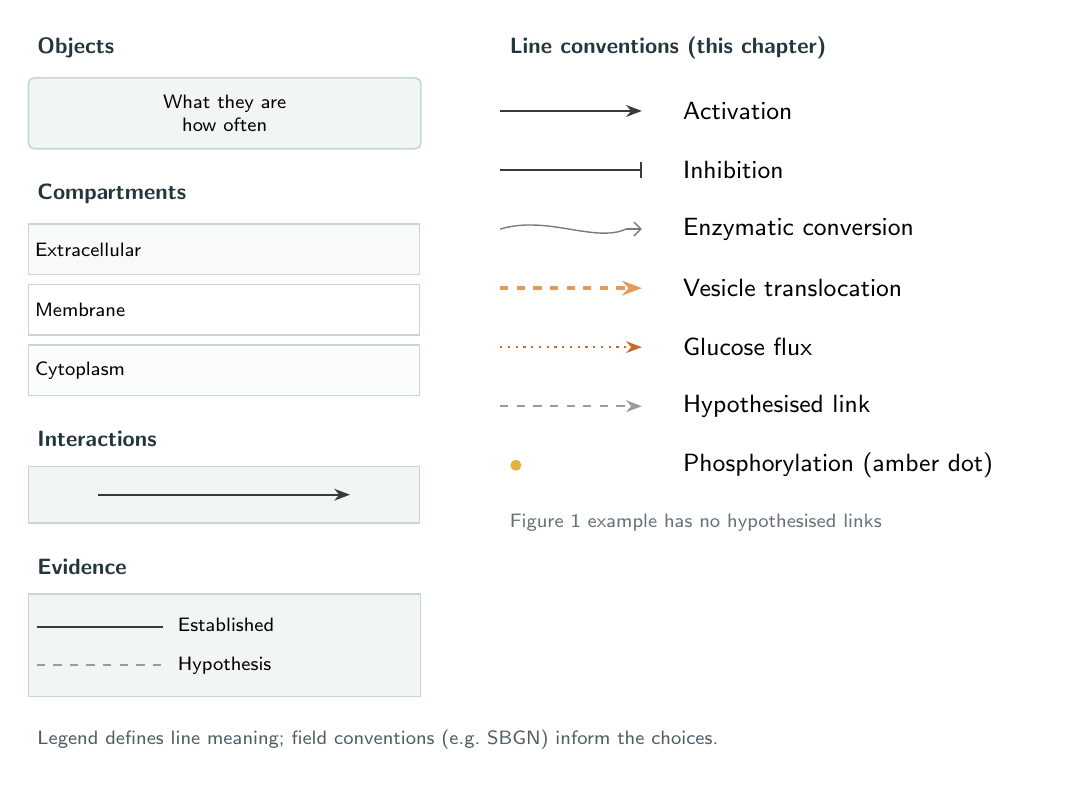
\begin{tikzpicture}[
  font=\sffamily\small,
  paneltitle/.style={font=\sffamily\bfseries\footnotesize, text=BookInk, anchor=west},
  foot/.style={font=\sffamily\scriptsize, text=BookInk!80},
  infobox/.style={
    draw=BookRule, line width=0.6pt, rounded corners=2pt, fill=BookPale,
    font=\sffamily\scriptsize, align=center,
    text width=48mm, minimum height=9mm, inner sep=2.6pt
  },
  band/.style={
    draw=BookRule, line width=0.5pt,
    font=\sffamily\scriptsize, align=left,
    text width=48mm, minimum height=6.4mm, inner sep=2.4pt
  },
  evbox/.style={
    draw=BookRule, line width=0.5pt, fill=BookPale,
    font=\sffamily\scriptsize, align=left,
    text width=48mm, minimum height=13mm, inner sep=2.6pt
  },
]
\definecolor{ch07act}{HTML}{3A3A3A}
\definecolor{ch07conv}{HTML}{7A7A7A}
\definecolor{ch07trans}{HTML}{E39B5B}
\definecolor{ch07flux}{HTML}{C46A2A}
\definecolor{ch07phos}{HTML}{E3B23C}
\definecolor{ch07hyp}{HTML}{9A9A9A}

\node[paneltitle] (tObj) at (0,0) {Objects};
\node[infobox, anchor=north west] (bObj) at ([yshift=-1.2mm]tObj.south west) {What they are\\how often};

\node[paneltitle, anchor=north west] (tComp) at ([yshift=-3.2mm]bObj.south west) {Compartments};
\node[band, fill=BookPale!50, anchor=north west] (bExt) at ([yshift=-1.2mm]tComp.south west) {Extracellular};
\node[band, fill=white, anchor=north west] (bMem) at ([yshift=-1.1mm]bExt.south west) {Membrane};
\node[band, fill=BookPale!30, anchor=north west] (bCyt) at ([yshift=-1.1mm]bMem.south west) {Cytoplasm};

\node[paneltitle, anchor=north west] (tInt) at ([yshift=-3.2mm]bCyt.south west) {Interactions};
\node[band, fill=BookPale, minimum height=7.2mm, align=center, anchor=north west]
  (bInt) at ([yshift=-1.2mm]tInt.south west)
  {\tikz[baseline=-0.55ex]{\draw[-{Stealth[length=2mm]}, ch07act, line width=0.8pt] (0,0) -- (32mm,0);}};

\node[paneltitle, anchor=north west] (tEv) at ([yshift=-3.2mm]bInt.south west) {Evidence};
\node[evbox, anchor=north west] (bEv) at ([yshift=-1.2mm]tEv.south west) {%
  \begin{tabular}{@{}l@{\hspace{1.8mm}}l@{}}
    \tikz[baseline=-0.55ex]{\draw[ch07act, line width=0.8pt] (0,0) -- (16mm,0);} & Established \\[1.4mm]
    \tikz[baseline=-0.55ex]{\draw[ch07hyp, line width=0.8pt, dashed] (0,0) -- (16mm,0);} & Hypothesis
  \end{tabular}};

\node[paneltitle] (rt) at (60mm,0) {Line conventions (this chapter)};
\draw[-{Stealth[length=2mm]}, ch07act, line width=0.8pt] (60mm,-8mm) -- (78mm,-8mm);
\node[anchor=west, font=\sffamily\small] at (82mm,-8mm) {Activation};
\draw[-{Bar[width=6pt]}, ch07act, line width=0.8pt] (60mm,-15.5mm) -- (78mm,-15.5mm);
\node[anchor=west, font=\sffamily\small] at (82mm,-15.5mm) {Inhibition};
\draw[ch07conv, line width=0.5pt] (60mm,-23mm) .. controls (66mm,-21.2mm) and (72mm,-24.8mm) .. (76mm,-23mm);
\draw[-{Straight Barb[open]}, ch07conv, line width=0.5pt] (76mm,-23mm) -- (78mm,-23mm);
\node[anchor=west, font=\sffamily\small] at (82mm,-23mm) {Enzymatic conversion};
\draw[ch07trans, line width=1.5pt, dashed, -{Stealth[length=2.5mm, open]}] (60mm,-30.5mm) -- (78mm,-30.5mm);
\node[anchor=west, font=\sffamily\small] at (82mm,-30.5mm) {Vesicle translocation};
\draw[ch07flux, line width=0.8pt, dotted, -{Stealth[length=2mm]}] (60mm,-38mm) -- (78mm,-38mm);
\node[anchor=west, font=\sffamily\small] at (82mm,-38mm) {Glucose flux};
\draw[ch07hyp, line width=0.8pt, dashed, -{Stealth[length=2mm]}] (60mm,-45.5mm) -- (78mm,-45.5mm);
\node[anchor=west, font=\sffamily\small] at (82mm,-45.5mm) {Hypothesised link};
\fill[ch07phos] (62mm,-53mm) circle (2pt);
\node[anchor=west, font=\sffamily\small] at (82mm,-53mm) {Phosphorylation (amber dot)};
\node[anchor=north west, font=\sffamily\scriptsize, text=BookInk!70, align=left, text width=68mm]
  at (60mm,-58mm) {Figure~1 example has no hypothesised links};

\node[foot, anchor=north west] at ([yshift=-3mm]current bounding box.south west)
  {Legend defines line meaning; field conventions (e.g.\ SBGN) inform the choices.};
\end{tikzpicture}

\caption{The four kinds of information a mechanism figure must state, and the line conventions used in this chapter. Each relation type gets exactly one line style, and hypothesised links must be distinguishable from established ones. The legend, informed by field conventions, defines what each line means.}\label{fig:ch07-01}
\end{figure}

\textbf{First, objects: what each entity is and how many times it appears.} Every shape in a schematic represents a conceptual entity---a ligand, transmembrane receptor, intracellular kinase, membrane lipid, or storage vesicle. When the same molecule appears twice in one diagram, a reader naturally asks whether the duplication represents two subunits, two conformational states, or two locations before and after transport. Without strict multiplicity rules, image models routinely duplicate icons to fill space, such as lining up six identical transporter barrels in one membrane pit. An object inventory must therefore specify both identity and count. Any node acting at a single step (the insulin receptor, IRS-1, PI3K, PDK1, Akt, mTORC2, AS160) should appear once. Only when the mechanism involves spatial relocation may an object appear twice: GLUT4 is shown once embedded in intracellular storage vesicles (reserve state) and once inserted into the plasma membrane (active state), drawn with identical geometry and colour.

Object design also requires only ``necessary structural detail.'' A pathway schematic clarifies causal logic rather than atomic structure. Include only morphological features that affect mechanistic understanding: the insulin receptor must span the bilayer to transmit an extracellular signal indoors, and Rab must sit on the storage vesicle surface where it acts. By contrast, drawing the disulfide-linked $\alpha_2\beta_2$ tetramer details of the insulin receptor or the p85/p110 subunit interface of PI3K adds clutter and invites model distortion; such features are better simplified into clean silhouettes and noted in the caption.

\textbf{Second, compartments: spatial partitioning is itself scientific information.} Treating membranes, phase boundaries, or organelles as decorative backdrops is a primary source of localization error. In insulin signaling, insulin remains in the extracellular space contacting the receptor ectodomain; phosphatidylinositol 4,5-bisphosphate ($\text{PIP}_2$) and 3,4,5-trisphosphate ($\text{PIP}_3$) are anchored in the inner leaflet of the plasma membrane rather than floating in the cytosol; and PDK1 and Akt must bind inner-leaflet $\text{PIP}_3$ via their PH domains to be activated, so both belong directly against the cytoplasmic face of the membrane. Dividing the canvas into explicit zones---extracellular space, plasma membrane, and cytoplasm---turns two-dimensional coordinates into a verifiable statement of subcellular localization.

\textbf{Third, interactions: assign exactly one line style to each relation type.} Many drafts suffer from arrow overloading, using one solid arrow for kinase phosphorylation, lipid conversion, vesicle movement, and transmembrane flux alike. When distinct processes share one symbol, readers must guess the mechanism; worse, using a pointed arrowhead for an inhibitory step turns negative regulation into activation.

The core principle of the Systems Biology Graphical Notation (SBGN; Le Nov\`ere et al., 2009; see also the official SBGN website) is to assign each interaction class a mutually exclusive glyph. Without adopting the full engineering syntax of SBGN, authors should establish a self-consistent line dictionary within every figure. Our main case study distinguishes five interaction styles and one state marker (Figure~\ref{fig:ch07-01}, right):
\begin{itemize}
\item \textbf{Direct binding and membrane recruitment:} Geometric contact without an arrow (insulin touching the receptor top; PDK1 and Akt touching the inner leaflet at $\text{PIP}_3$), reducing arrow clutter.
\item \textbf{Activation or stimulation:} Solid dark-grey line with a filled triangular head for positive regulation between signaling proteins.
\item \textbf{Inhibition:} Solid dark-grey line of the same weight ending in a perpendicular flat bar (T-bar) touching the target outline.
\item \textbf{Enzymatic chemical conversion:} Thinner mid-grey curved arc with an open V head from substrate to product, met at its midpoint by a short stub from the enzyme.
\item \textbf{Spatial translocation:} Thick dashed soft-orange arrow with a large open head representing physical movement of vesicles to the membrane.
\item \textbf{Transmembrane substance flux:} Dotted dark-orange line with a small filled head passing through the transporter channel to show glucose influx.
\item \textbf{Phosphorylation state:} Small amber dots on phosphorylated proteins rather than baked-in ``P'' letters, defined in the legend.
\end{itemize}

No line style has universal meaning outside its context. Because conventions vary across fields, every schematic must include an on-canvas legend and restate the definitions in the caption.

\textbf{Fourth, evidence status: separate established consensus, readability simplifications, and working hypotheses.} Mechanism figures often mix textbook facts, deliberate omissions for legibility, and newly proposed hypotheses. Drawing all three as identical solid lines invites reviewers to fault the figure for overstating speculation or omitting known branches. Instead, draw consensus steps as solid lines, declare omitted isoforms or parallel branches in the caption, and render hypothetical links as mid-grey dashed arrows labelled ``Hypothesised link'' in both legend and caption.

\section{From Relation Table to Sketch}

With these four requirements set, the next step is not to write an English prompt directly, but to organize the source material into a relation table as introduced in Chapter 2. We illustrate this using the canonical insulin-stimulated GLUT4 translocation pathway in skeletal muscle or adipose cells.

Suppose we are preparing Figure 1 of a paper to orient peers to this classic pathway. The figure reports no new data or hypotheses; every link rests on established reviews and primary studies (Saltiel and Kahn, 2001; Leto and Saltiel, 2012; Klip et al., 2019; Sano et al., 2003 for AS160; Sarbassov et al., 2005 for mTORC2). Listing thirteen protein names alone tells neither a human nor an AI who acts upstream or who inhibits whom. Writing them as the thirteen rows (R1--R13) of Table~\ref{tab:ch07-01} fixes every source, target, line style, compartment, and simplification.

\begin{table}[htbp]\centering\scriptsize
\setlength{\tabcolsep}{3pt}
\renewcommand{\arraystretch}{0.95}
\caption{Relation table (R1--R13) for insulin-stimulated GLUT4 translocation. Each row corresponds to one contact or connecting line in the figure.}\label{tab:ch07-01}
\begin{tabularx}{\linewidth}{lYYYYY}
\toprule
\textbf{ID} & \textbf{Source} & \textbf{Target / outcome} & \textbf{Relation \& line style} & \textbf{Compartment} & \textbf{Status \& simplification} \\
\midrule
R1 & Insulin & Insulin receptor (IR) & Binding (direct contact, no arrow) & Extracellular / outer membrane & Established; transmembrane dimer outline, omit $\alpha_2\beta_2$ details \\
R2 & Bound IR & IR kinase domain & Auto-phosphorylation (2 amber dots) & Cytoplasmic face of membrane & Established; omit specific Tyr residue numbers \\
R3 & Active IR & IRS-1 & Phosphorylation activation (solid arrow + 1 dot) & Sub-membrane cytoplasm & Established; IRS-1/2 both act in muscle/fat, show IRS-1 only \\
R4 & Phospho-IRS-1 & Class IA PI3K & Recruitment \& activation (solid arrow) & Sub-membrane cytoplasm & Established; do not split p85 and p110 subunits \\
R5 & PI3K & $\text{PIP}_2 \rightarrow \text{PIP}_3$ & Enzymatic conversion (thin arc, open V head, PI3K stub at midpoint) & Inner leaflet of membrane & Established; omit PTEN and SHIP2 dephosphorylation \\
R6 & $\text{PIP}_3$ & PDK1 and Akt & Membrane recruitment (touch inner leaflet, no arrow) & Inner leaflet of membrane & Established; omit PH domain, express by membrane contact \\
R7 & PDK1 & Akt & Thr308 phosphorylation (solid arrow) & Inner face of membrane & Established; shares 2 amber dots on Akt with R8 \\
R8 & mTORC2 & Akt & Ser473 phosphorylation (solid arrow) & Sub-membrane cytoplasm & Established (Sarbassov et al., 2005); no upstream arrow into mTORC2 \\
R9 & Active Akt & AS160 (TBC1D4) & Phosphorylation \& GAP inhibition (T-bar + 1 dot) & Cytoplasm & Established (Sano et al., 2003); omit 14-3-3 and TBC1D1 \\
R10 & AS160 & Vesicle Rab & Inhibition of Rab activity (T-bar touching Rab) & Storage vesicle surface & Established; do not distinguish Rab8A/10/13 isoforms \\
R11 & Rab-GTP & GLUT4 storage vesicles (GSVs) & Promotion of translocation (thick dashed orange arrow, open head) & Cytoplasm $\rightarrow$ membrane & Established; omit microtubules, actin, and motor proteins \\
R12 & Translocated GSVs & Membrane GLUT4 & Membrane fusion \& insertion (dashed arrow ends at membrane GLUT4) & Plasma membrane & Established; omit VAMP2/syntaxin-4 SNARE proteins \\
R13 & Extracellular glucose & Intracellular glucose & Facilitated diffusion via GLUT4 (dotted dark-orange arrow downward) & Extracellular $\rightarrow$ cytoplasm & Established; omit hexokinase and downstream glycolysis \\
\bottomrule
\end{tabularx}
\end{table}

Below the table we also record an explicit exclusion list of what not to draw: the Grb2--SOS--Ras--MAPK mitogenic branch; the debated CAP--Cbl--TC10 branch; GLUT4 endocytosis and recycling; S6K negative feedback and contraction-activated AMPK signaling (Leto and Saltiel, 2012; Klip et al., 2019); and any quantitative data. Stating what to omit both constrains the AI prompt and prepares the simplification disclosure in the figure legend.

From Table~\ref{tab:ch07-01}, five minutes with a pencil yields a layout sketch (V0) placing all thirteen relations into two-dimensional space (Figure~\ref{fig:ch07-02}). A sketch fixes only compartments and reading order: a horizontal double line across the top fifth represents the plasma membrane, separating extracellular space, membrane, and cytoplasm. The main cascade runs left to right just below the membrane from the receptor to Akt, steps down and right via two consecutive T-bars to the vesicle cluster, and curves upward via a thick dashed arrow to the membrane GLUT4 beneath the downward dotted glucose line---forming a ``left $\rightarrow$ right, then lower-right $\rightarrow$ upper-right'' trajectory while reserving the bottom tenth for a legend.

\begin{figure}[htbp]\centering
% FIG ch07-02 relation-number overlay (language-neutral)
\makeatletter
\@ifundefined{chsevenrelmark}{%
\newcommand{\chsevenrelmark}[2][]{%
  \tikz[baseline=(char.base)]{%
    \node[shape=circle, draw=BookInk, line width=0.5pt, fill=white, inner sep=1pt,
      font=\fontsize{7}{7}\selectfont, #1] (char) {#2};}}%
}{}
\makeatother
\begin{tikzpicture}
  \node[anchor=south west, inner sep=0] (img) at (0,0)
    {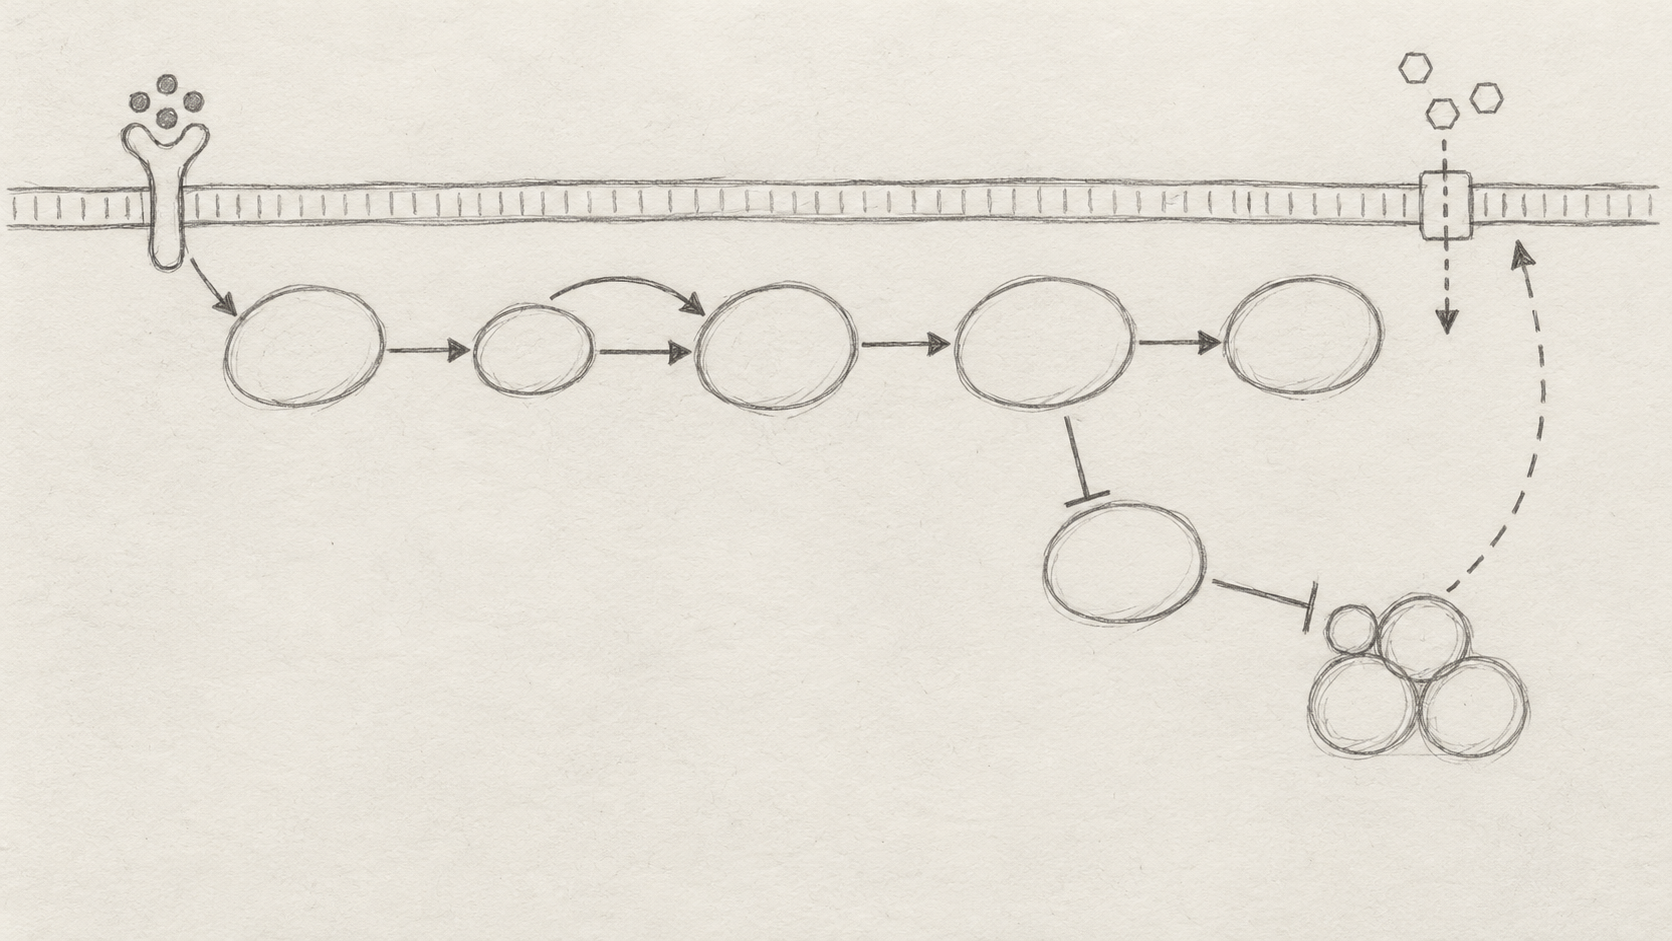
\includegraphics[width=\linewidth]{figures/ch07/ch07-02-v0-sketch.png}};
  \begin{scope}[x={(img.south east)}, y={(img.north west)}]
    \node at (0.12, 1-0.10) {\chsevenrelmark{1}};
    \node at (0.12, 1-0.28) {\chsevenrelmark{2}};
    \node at (0.17, 1-0.44) {\chsevenrelmark{3}};
    \node at (0.25, 1-0.42) {\chsevenrelmark{4}};
    \node at (0.37, 1-0.26) {\chsevenrelmark{5}};
    \node at (0.47, 1-0.37) {\chsevenrelmark{7}};
    \node at (0.53, 1-0.50) {\chsevenrelmark{8}};
    \node at (0.58, 1-0.46) {\chsevenrelmark{9}};
    \node at (0.67, 1-0.58) {\chsevenrelmark{10}};
    \node at (0.80, 1-0.45) {\chsevenrelmark{11}};
    \node at (0.87, 1-0.24) {\chsevenrelmark{12}};
    \node at (0.88, 1-0.12) {\chsevenrelmark{13}};
    \node at (0.44, 1-0.36) {\chsevenrelmark{6}};
  \end{scope}
\end{tikzpicture}

\caption{A planning sketch laid out from the relation table (a pencil sketch simulated by an image model, not a real manuscript page). Circled numbers map to relations R1--R13 in Table~\ref{tab:ch07-01}. The sketch fixes compartments, rough positions and reading order only; used as input for generation, it conveys layout intent and does not lock the layout.}\label{fig:ch07-02}
\end{figure}

The base image of Figure~\ref{fig:ch07-02} was generated by an image model simulating a pencil sketch, with circled numbers (1)--(13) overlaid in TikZ. Even for a rough sketch, running the same prompt three times exposed typical model drift: the first two runs drew only one T-bar and left the lower-right vesicle regulator disconnected from the main chain. Only on the third run---after we added an explicit instruction requiring two consecutive T-bars connecting the fourth main-chain blob to the lower-right blob and the vesicle-surface bead---did the series of (9) and (10) appear as in Figure~\ref{fig:ch07-02}. At the same time, the model dropped the upward mTORC2 blob below Akt, drew the glucose path (13) as short dashes rather than dots, and left a tiny gap between the insulin dots (1) and the receptor.

This clarifies the role of a sketch: it carries no molecular names, helping the author and tool align on compartments and flow. In \scidraw{}, an author can upload a sketch in sketch mode alongside a text brief to generate a draft, but sketch conditioning expresses layout intent rather than rigid object locking, so the output must still be checked row by row against Table~\ref{tab:ch07-01}.

\section{Why One Sentence Is Not Enough}

To see how input completeness governs scientific accuracy, we can compare the output of our opening one-sentence prompt (V1) against a draft driven by a complete figure brief (V2) under identical generation settings (Figure~\ref{fig:ch07-03}).

When working in \scidraw{}, the recommended starting point is to save a structured brief derived from your relation table in your own document, then open the Scientific Figure Workflow wizard (\sdtool{figure-workflow}), choose ``Mechanism \& workflow diagram'', and follow the route into the mechanism generator (\sdtool{mechanism-figure-generator}) or prompt drawing tool (\sdtool{ai-drawing}), pasting the brief in. Remember that the workflow wizard only lines up the tools in order; it does not verify biochemical accuracy on your behalf. The core sections of our structured figure brief read as follows (the full brief is archived in the \texttt{cases/} directory of the book repository):

\begin{Prompt}
[Purpose & Audience] Journal Figure 1 background schematic (double-column width 174 mm,
height ~100 mm) for metabolism and cell-biology readers.
[Goal] Show the signaling sequence Insulin -> IR -> IRS-1 -> PI3K -> PIP3 -> Akt, the
double inhibition Akt -| AS160 -| Rab, and the resulting GSV translocation, membrane
fusion, and glucose influx, without presenting any experimental data or new hypotheses.
[Objects & Counts] Each object appears once except GLUT4 (shown in vesicles and membrane):
Extracellular: insulin (3 beads), glucose (4 hexagons). Plasma membrane: lipid bilayer,
insulin receptor dimer, inner-leaflet PIP2 & PIP3, inserted GLUT4 (1 barrel).
Cytoplasm: IRS-1, PI3K, PDK1, Akt, mTORC2, AS160, vesicle-bound Rab, GSV cluster (3 vesicles).
Amber phosphorylation dots on IR (2), IRS-1 (1), Akt (2), and AS160 (1); no "P" letters.
[Relations & Line Styles] R1 insulin contacts IR (no arrow); R2 IR autophosphorylation;
R3 IR -> IRS-1, R4 IRS-1 -> PI3K, R7 PDK1 -> Akt, R8 mTORC2 -> Akt as solid dark-grey
activation arrows (no upstream arrow into mTORC2); R5 PI3K catalyses PIP2 -> PIP3 via thin
arc with open V head (PI3K stub at midpoint); R6 PIP3 recruits PDK1 & Akt to inner leaflet;
R9 Akt -| AS160 and R10 AS160 -| Rab as perpendicular T-bars; R11-R12 GSV translocation
to membrane GLUT4 as thick dashed orange arrow; R13 glucose influx as dotted orange arrow.
[Layout & Visuals] 16:9 landscape; top 20% extracellular, 20-28% membrane, 28-88% cytoplasm,
bottom 12% blank for legend. Flat 2D vector style on white; medium blue for signaling
proteins, grey-blue for AS160/Rab, soft orange for GLUT4/GSVs/glucose, warm grey membrane.
[Restrictions] Strictly no text, letters, or numbers in the base image; no nucleus, ER,
Golgi, cytoskeleton, MAPK or CAP-Cbl-TC10 branches, endocytosis, or decorative effects.
\end{Prompt}

For the counterexample V1, we submitted only the single vague sentence from the opening vignette:

\begin{Prompt}
Make a beautiful, professional scientific illustration of insulin signaling and
GLUT4 translocation for a top journal.
\end{Prompt}

For the brief-driven draft V2, we translated the structured brief into an explicit English image prompt specifying spatial bands (\texttt{SPACE}), the thirteen objects with their relative positions and counts (\texttt{OBJECTS}), the five mutually exclusive line styles (\texttt{RELATIONS}), and the forbidden elements (\texttt{DO NOT DRAW}), while prohibiting all text (full prompt in the \texttt{cases/} directory; key excerpt below):

\begin{Prompt}
Flat 2D scientific schematic for a journal figure, landscape 16:9, pure white
background. Clean vector style, flat fills, thin dark outlines, no gradients,
no shadows, no 3D. ABSOLUTELY NO TEXT: no letters, words, numbers, or symbols.
SPACE: Top 20% = extracellular; 20-28% = horizontal lipid bilayer membrane;
28-88% = cytoplasm; bottom 12% = empty white strip reserved for legend.
OBJECTS (each appears once; GLUT4 appears in vesicles and in plasma membrane):
1. Insulin (3 dark-blue beads touching receptor); 2. Transmembrane receptor (2 amber dots);
3. IRS-1 (1 amber dot); 4. PI3K; 5. Inner-leaflet PIP2 & PIP3; 6. PDK1 & 7. Akt
   (both touching inner leaflet at PIP3; Akt has 2 amber dots); 8. mTORC2 below Akt;
9. AS160 (gray-blue, 1 amber dot); 10. GSV cluster (3 vesicles with orange GLUT4 barrels);
11. Rab bead on vesicle; 12. GLUT4 in right plasma membrane; 13. Glucose hexagons above it.
RELATIONS (draw only these):
- Activation (solid dark-gray line, filled triangle): IR -> IRS-1 -> PI3K; PDK1 -> Akt; mTORC2 -> Akt.
- Inhibition (solid dark-gray line, perpendicular T-bar): Akt -| AS160; AS160 -| Rab.
- Enzymatic conversion (thin mid-gray arc, open V head): PIP2 -> PIP3, PI3K stub touching midpoint.
- Translocation (thick dashed orange arrow, open head): GSV cluster upward to membrane GLUT4.
- Substance flow (dotted dark-orange arrow): extracellular glucose through membrane GLUT4 into cell.
\end{Prompt}

\begin{figure}[htbp]\centering
% FIG ch07-03a V1 error markers (language-neutral)
\definecolor{ch07err}{HTML}{C0392B}
\makeatletter
\@ifundefined{chsevenerrmark}{%
\newcommand{\chsevenerrmark}[2][]{%
  \tikz[baseline=(char.base)]{%
    \node[shape=circle, fill=ch07err, text=white, inner sep=1.5pt,
      font=\fontsize{7}{7}\selectfont\bfseries, #1] (char) {#2};}}%
}{}
\makeatother
\begin{tikzpicture}
  \node[anchor=south west, inner sep=0] (img) at (0,0)
    {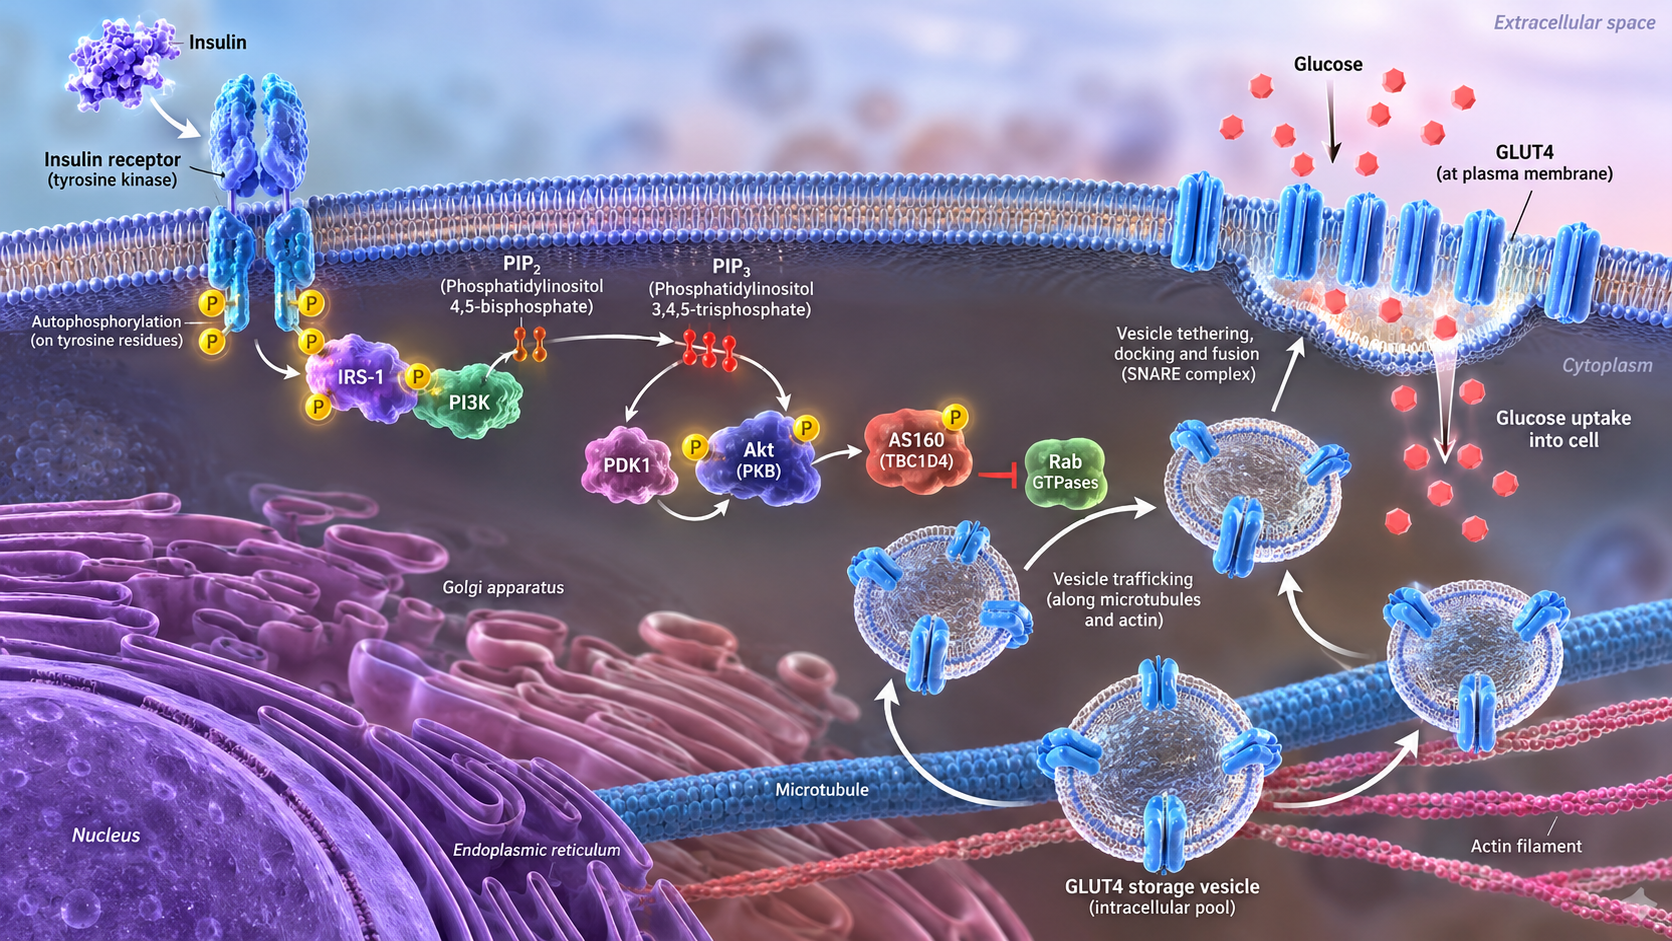
\includegraphics[width=\linewidth]{figures/ch07/ch07-03a-v1-vague.png}};
  \begin{scope}[x={(img.south east)}, y={(img.north west)}]
    \node at (0.14, 1-0.18) {\chsevenerrmark{1}};
    \node at (0.72, 1-0.22) {\chsevenerrmark{2}};
    \node at (0.50, 1-0.35) {\chsevenerrmark{3}};
    \node at (0.38, 1-0.55) {\chsevenerrmark{4}};
    \node at (0.55, 1-0.72) {\chsevenerrmark{5}};
    \node at (0.22, 1-0.48) {\chsevenerrmark{6}};
    \node at (0.82, 1-0.40) {\chsevenerrmark{7}};
  \end{scope}
\end{tikzpicture}


\vspace{2mm}
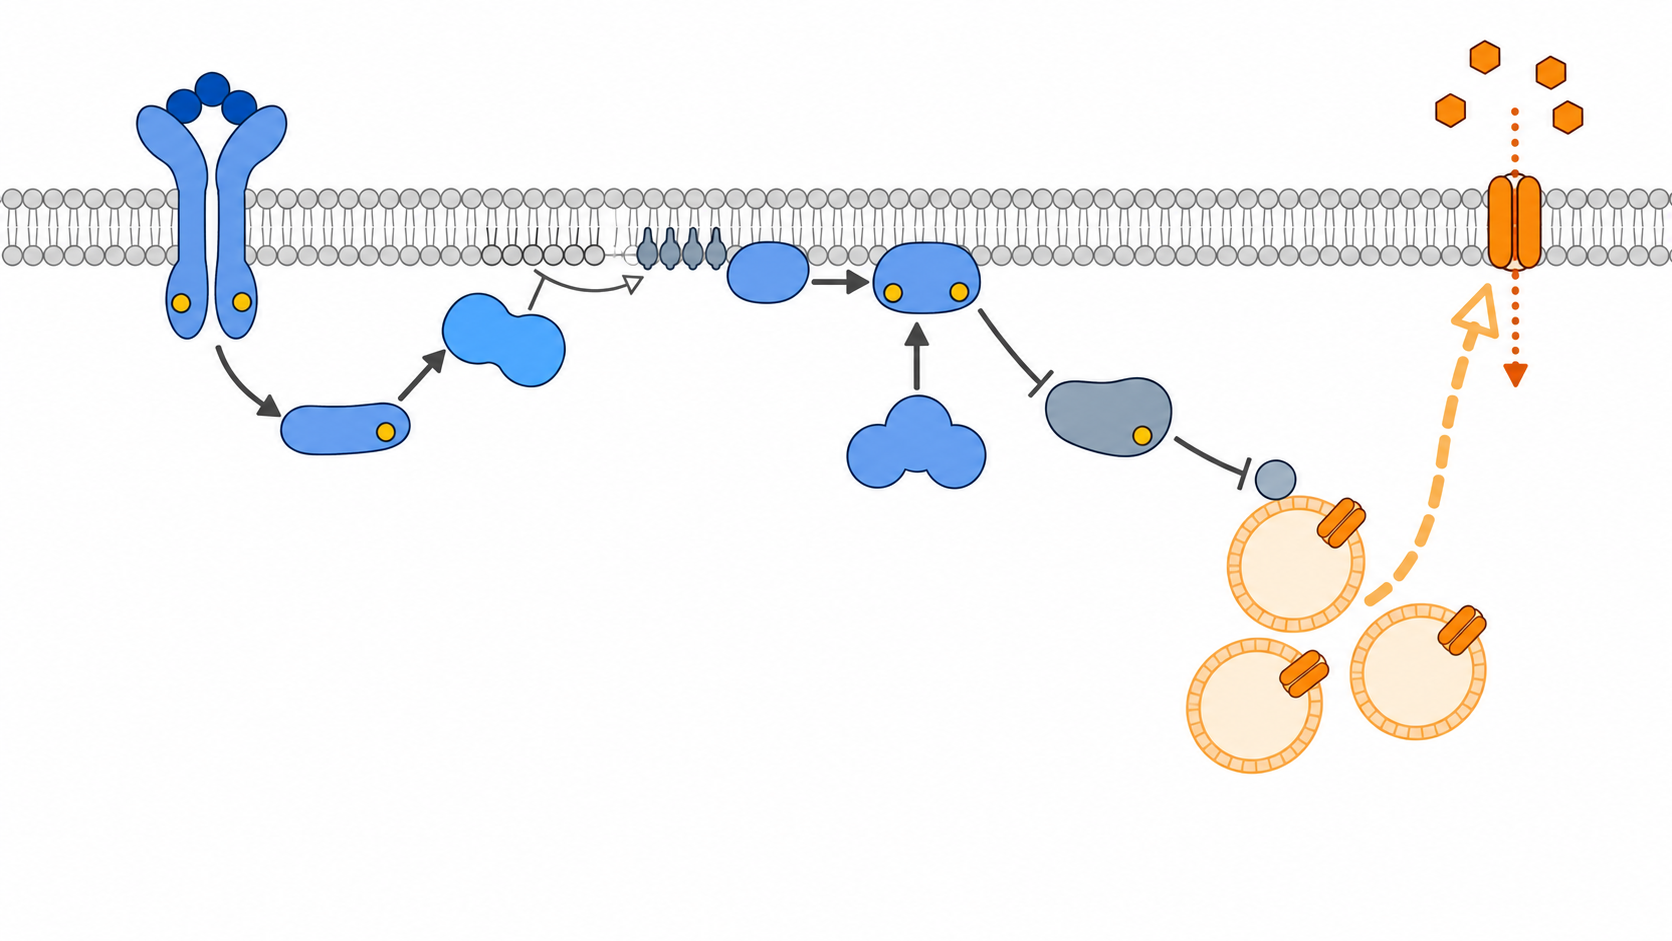
\includegraphics[width=\linewidth]{figures/ch07/ch07-03b-v2-brief.png}
\caption{Comparison of drafts generated from a one-sentence prompt versus a full figure brief. (a) A first draft from a one-sentence prompt; the model bakes rasterized text directly into a dark 3D background, and red numbers mark the scientific and graphical problems discussed in the text. (b) A text-free draft from the full brief: objects and relations can largely be checked one by one, while colour, line weight and spacing are not yet consistent. Example images in this chapter were produced by an image model; prompts and generation logs are available in the book repository.}\label{fig:ch07-03}
\end{figure}

Inspecting Figure~\ref{fig:ch07-03}a shows why surface polish can mislead. Although the model rendered mostly legible English labels rather than garbled pseudo-letters in this run, every word is baked directly into the dark, shaded bitmap. Reduced to a 174 mm double-column print width, small labels over glowing backgrounds become hard to read, and neither font size nor spelling can be edited later. More importantly, checking the image against Table~\ref{tab:ch07-01} exposes seven substantive errors (red circles 1--7 in Figure~\ref{fig:ch07-03}a):
\begin{enumerate}
\item \textbf{Incorrect ligand binding and excessive 3D styling (1):} Extracellular insulin points to the receptor via a white arrow instead of direct contact (violating R1), while heavy highlights, shadows, and glowing ``P'' orbs obscure protein boundaries.
\item \textbf{Multiplicity violation and baked-in prose (2):} Six blue GLUT4 channels crowd a single upper-right membrane pit (violating the single-node rule), alongside three lines of explanatory text about SNAREs baked into the cytosol.
\item \textbf{Inverted causal logic, missing branch, and localization errors (3):} First, \textbf{mTORC2 is completely missing} (omitting R8). Second, \textbf{Akt to AS160 is drawn as a solid white activation arrow} (violating R9), whereas AS160 to Rab uses a red T-bar (R10)---claiming that Akt \emph{activates} AS160 to \emph{inhibit} Rab, the exact opposite of biology! Furthermore, $\text{PIP}_3$ connects via arrows to PDK1 and Akt floating far from the membrane (violating R6), and the green Rab sphere floats free in the cytosol instead of sitting on a vesicle (violating R10).
\item \textbf{Irrelevant organelles filling half the canvas (4):} A huge nucleus, endoplasmic reticulum, and Golgi stack dominate the lower left, crowding the signaling pathway.
\item \textbf{Ambiguous cytoskeleton and looping vesicle arrows (5):} Microtubules and actin filaments fill the lower right while curved arrows connect four cut-away vesicles in a loop, obscuring the storage pool and translocation direction.
\item \textbf{Overlapping upstream nodes and faulty catalysis (6):} IRS-1 and PI3K overlap without a clear activation arrow (obscuring R4), and PI3K points at $\text{PIP}_2$ itself rather than the midpoint of the $\text{PIP}_2 \rightarrow \text{PIP}_3$ conversion arc (violating R5).
\item \textbf{Uniform arrows and missing legend (7):} Apart from one red T-bar, binding, catalysis, activation, vesicle movement, and glucose entry all share the same solid white arrow, with no legend.
\end{enumerate}

Why must both consecutive T-bars be kept in the Akt $\dashv$ AS160 $\dashv$ Rab segment (R9--R10)? In the basal state, AS160 has active Rab-GAP activity that keeps vesicle-associated Rab in its inactive GDP-bound form, acting like a brake that retains vesicles in the cytosol (Sano et al., 2003; Leto and Saltiel, 2012). Akt phosphorylates and \textbf{inhibits} AS160, releasing that brake so Rab remains GTP-bound and promotes vesicle translocation. Collapsing those steps into a single ``Akt $\rightarrow$ GSV'' shortcut arrow erases the mechanism, whereas drawing activation followed by inhibition (Figure~\ref{fig:ch07-03}a) reverses the causal sign.

Now examine Figure~\ref{fig:ch07-03}b, generated from the full brief. When we ran this prompt twice, the first candidate mistakenly routed the T-bar into AS160 from mTORC2 instead of Akt and placed two Rab beads on the vesicles; the second candidate (Figure~\ref{fig:ch07-03}b) fixed both connections. Here the ``extracellular--membrane--cytoplasm'' zones are clear, all thirteen objects and six amber phosphorylation dots are in place, and all five line styles are distinct without extra organelles or baked-in text. Structural accuracy comes from a complete brief paired with line-by-line verification.

\section{One Meaning per Line, One Role per Colour}

During refinement, two visual mistakes frequently creep in: varying arrow styles, weights, and colours arbitrarily, and painting every protein a different saturated hue. Two controlled comparisons illustrate the rules.

The first pair (Figure~\ref{fig:ch07-04}) isolates ``Akt $\dashv$ AS160 $\dashv$ Rab $\rightarrow$ vesicle translocation to membrane GLUT4.'' Figure~\ref{fig:ch07-04}a deliberately mixes four lines: a thick curved red filled arrow from the blue oval to the grey-blue shape (turning inhibition into activation), a thin green dashed open arrow from the grey-blue shape to the vesicle bead, a solid black filled arrow from the vesicles to the membrane transporter identical to a standard activation arrow (implying vesicles ``activate'' GLUT4), and an undefined purple double-headed arrow between the blue oval and the membrane. Figure~\ref{fig:ch07-04}b uses just three lines of two types: two equal-weight dark-grey T-bars in series for double inhibition, and one thick dashed soft-orange open-headed arrow curving upward for spatial translocation (zooming in still shows narrow gaps at the T-bar tips and slight shading on the shapes). Even without text, Figure~\ref{fig:ch07-04}b cleanly separates negative regulation from physical movement.

\begin{figure}[htbp]\centering
\begin{minipage}[t]{0.48\linewidth}\centering
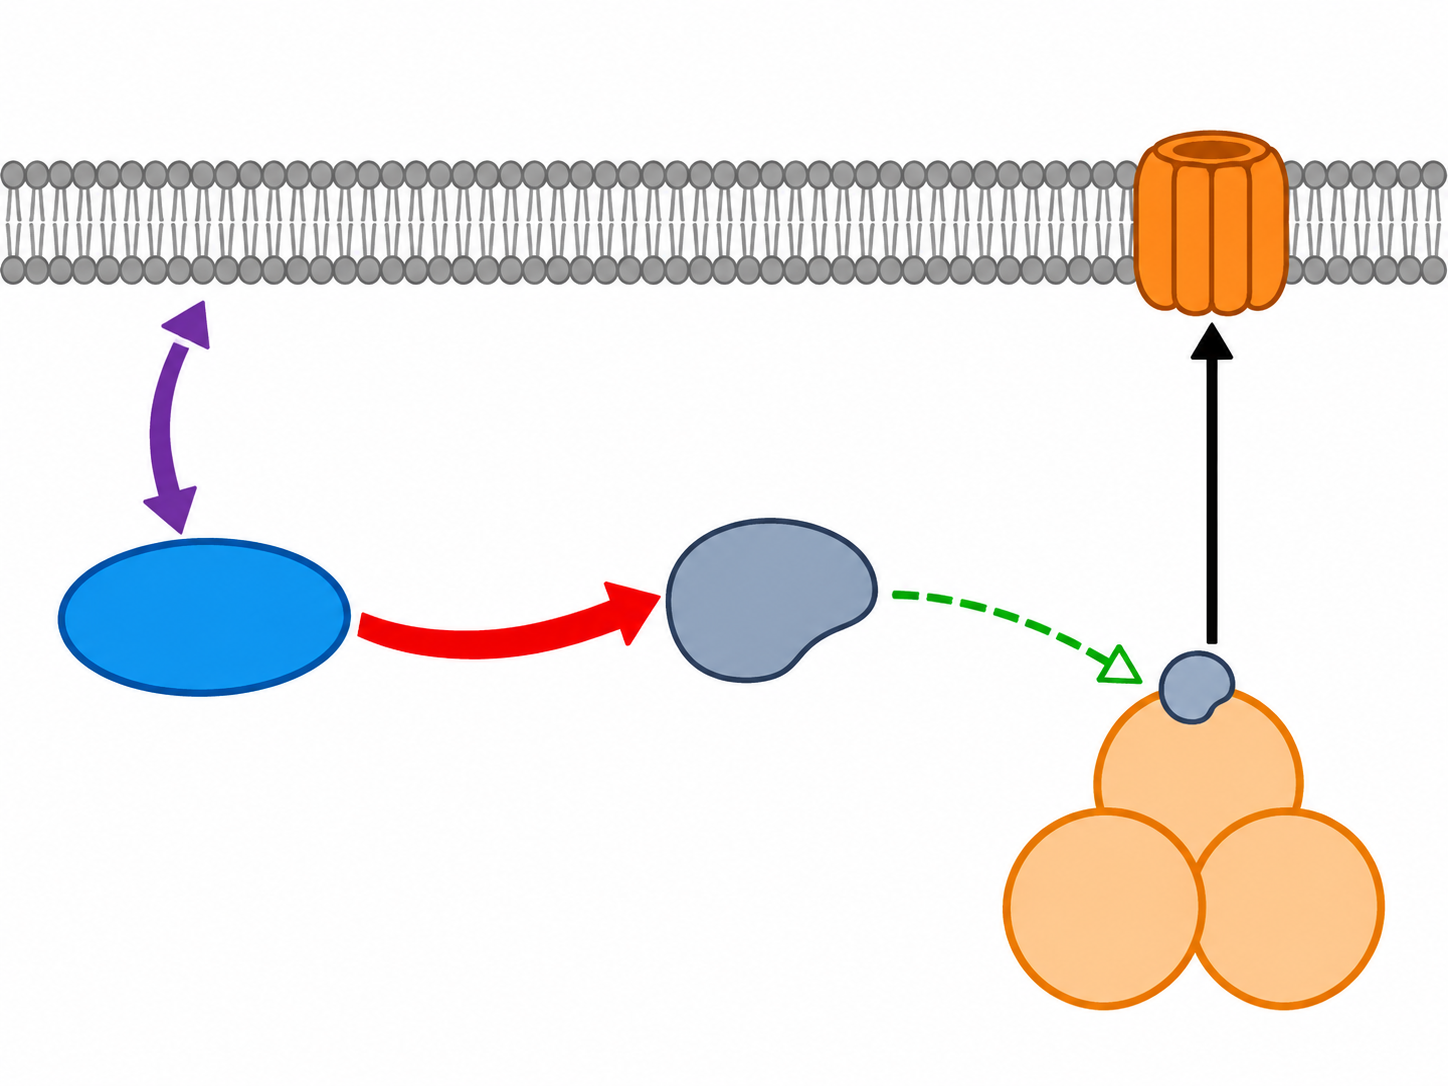
\includegraphics[width=\linewidth]{figures/ch07/ch07-04a-mixed-arrows.png}\\[1mm]
{\footnotesize (a) Mixed line styles: inhibition, translocation, and bidirectional arrows conflated}
\end{minipage}\hfill
\begin{minipage}[t]{0.48\linewidth}\centering
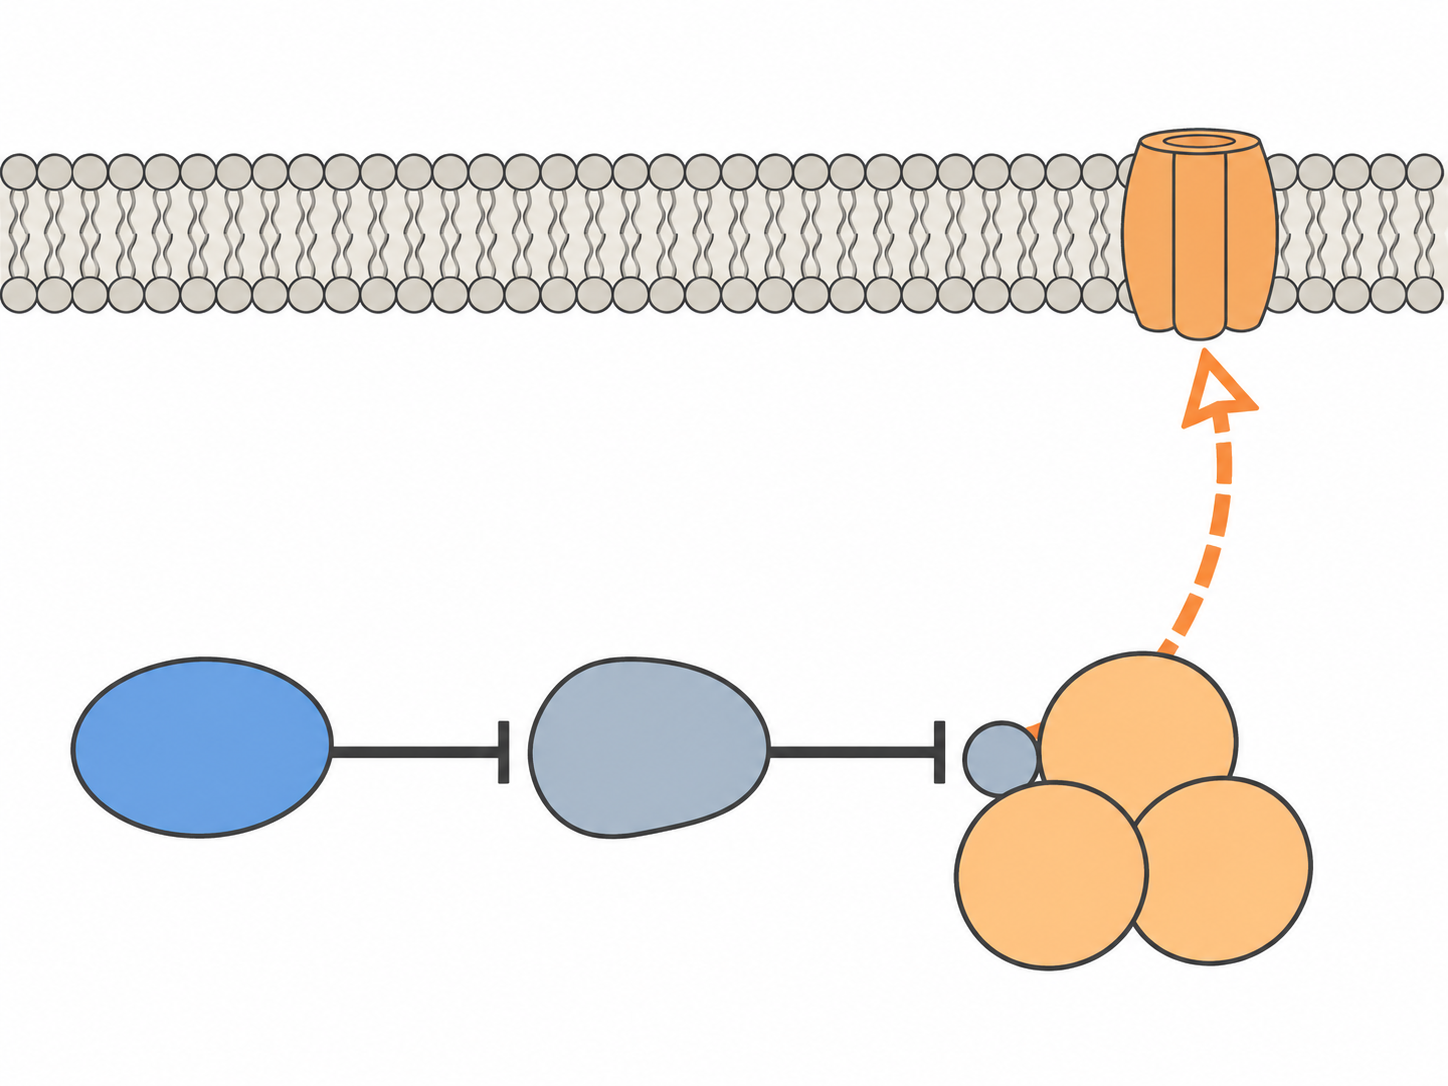
\includegraphics[width=\linewidth]{figures/ch07/ch07-04b-unified-arrows.png}\\[1mm]
{\footnotesize (b) Unified line semantics: two consecutive T-bars and one dashed translocation arrow}
\end{minipage}
\caption{Two drawings of the same simplified pathway. (a) Line style, colour and weight vary at random, the translocation arrow looks like an activation arrow, and a double-headed arrow has no defined meaning. (b) Two T-bars in series read as inhibition of an inhibitor, and the thick dashed arrow is the only symbol for spatial translocation.}\label{fig:ch07-04}
\end{figure}

The second pair (Figure~\ref{fig:ch07-05}) compares an overloaded palette against a restrained role-based palette, together with greyscale conversions.

\begin{figure}[htbp]\centering
\begin{minipage}[t]{0.48\linewidth}\centering
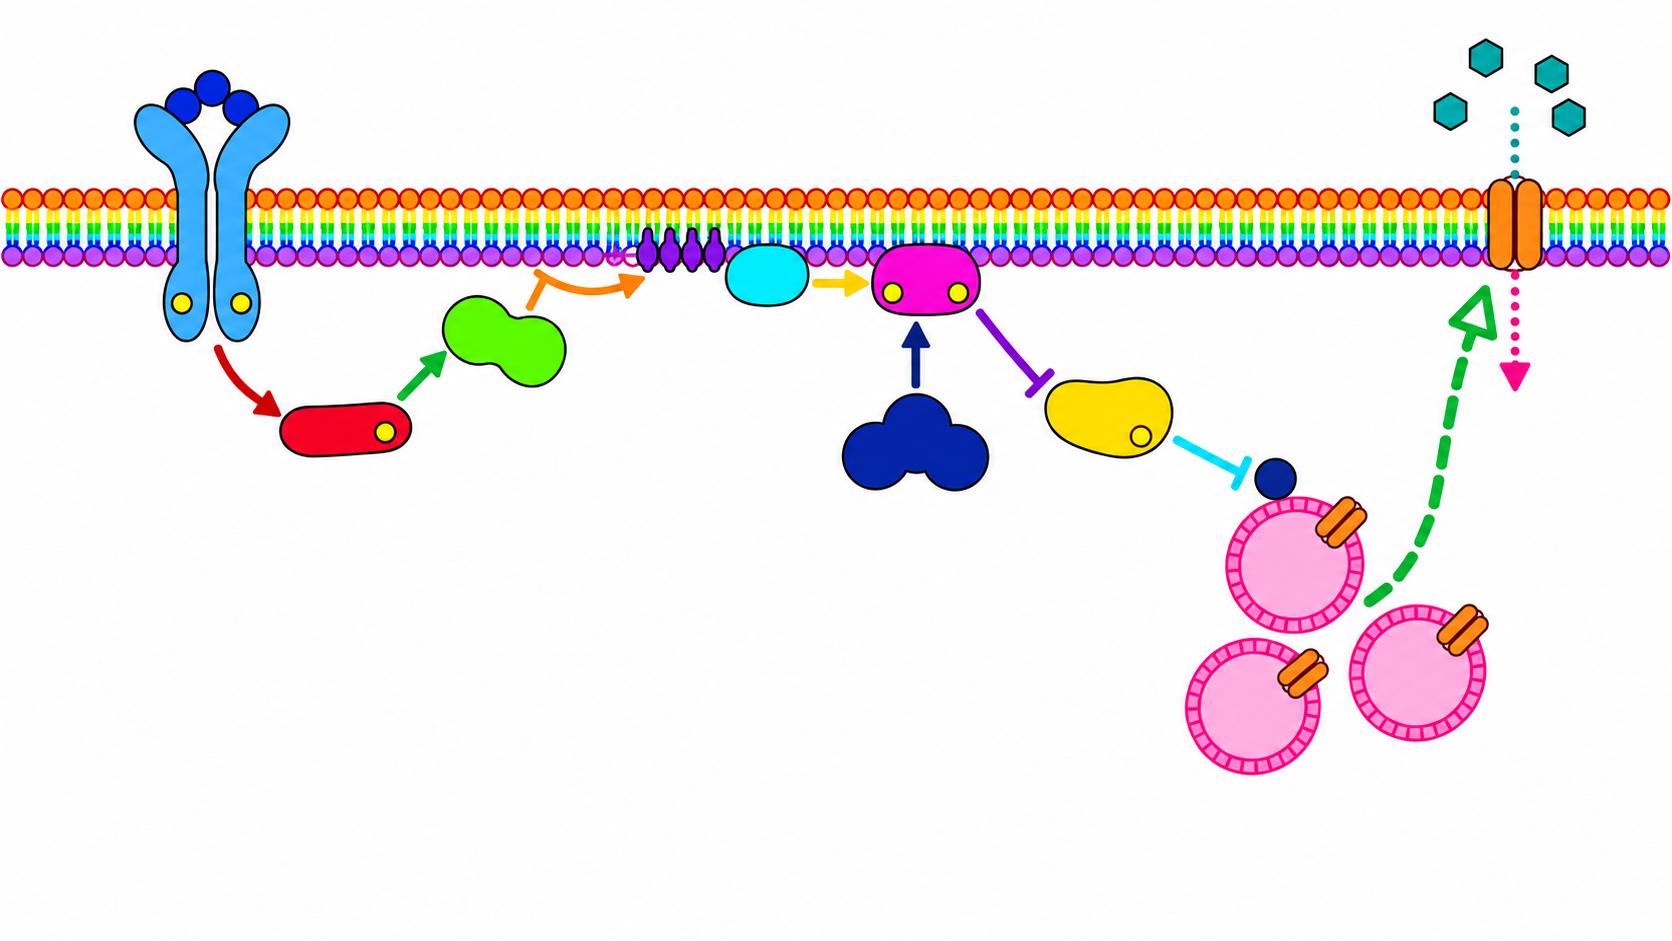
\includegraphics[width=\linewidth]{figures/ch07/ch07-05a-many-colours.png}\\[1mm]
{\footnotesize (a) Unrestrained palette: a different saturated hue per protein and a rainbow membrane}
\end{minipage}\hfill
\begin{minipage}[t]{0.48\linewidth}\centering
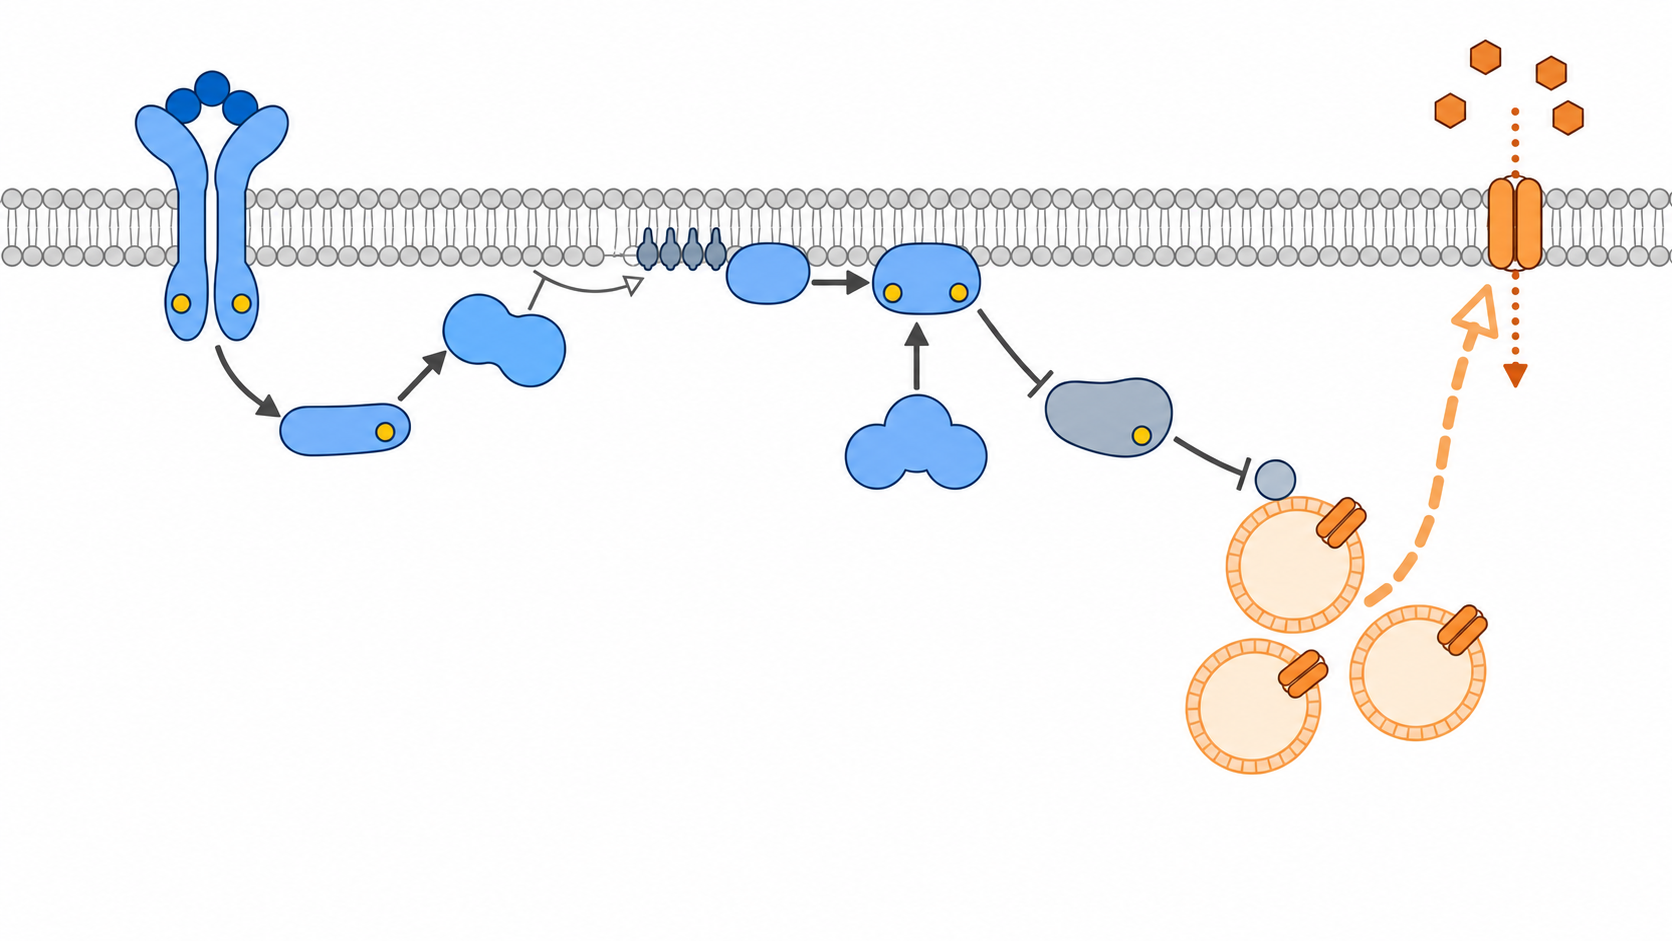
\includegraphics[width=\linewidth]{figures/ch07/ch07-05b-v3-revised.png}\\[1mm]
{\footnotesize (b) Restrained palette (V3): three functional hues plus neutral grey}
\end{minipage}

\vspace{2mm}
\begin{minipage}[t]{0.48\linewidth}\centering
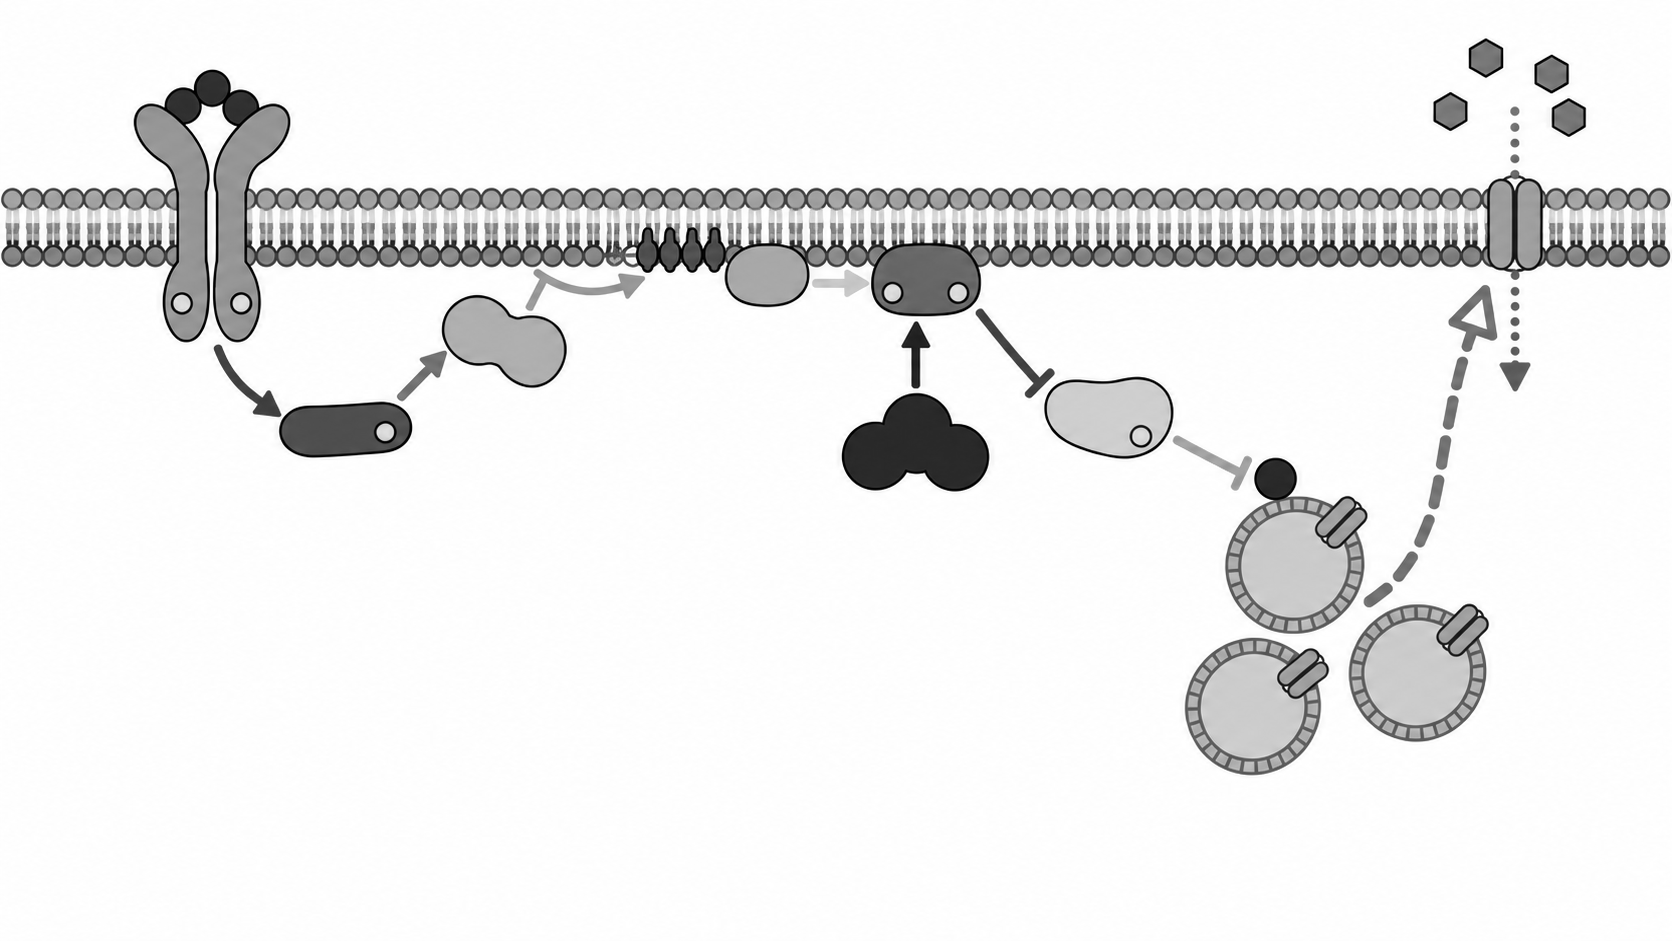
\includegraphics[width=\linewidth]{figures/ch07/ch07-05a-many-colours-gray.png}\\[1mm]
{\footnotesize (c) Greyscale conversion of panel (a)}
\end{minipage}\hfill
\begin{minipage}[t]{0.48\linewidth}\centering
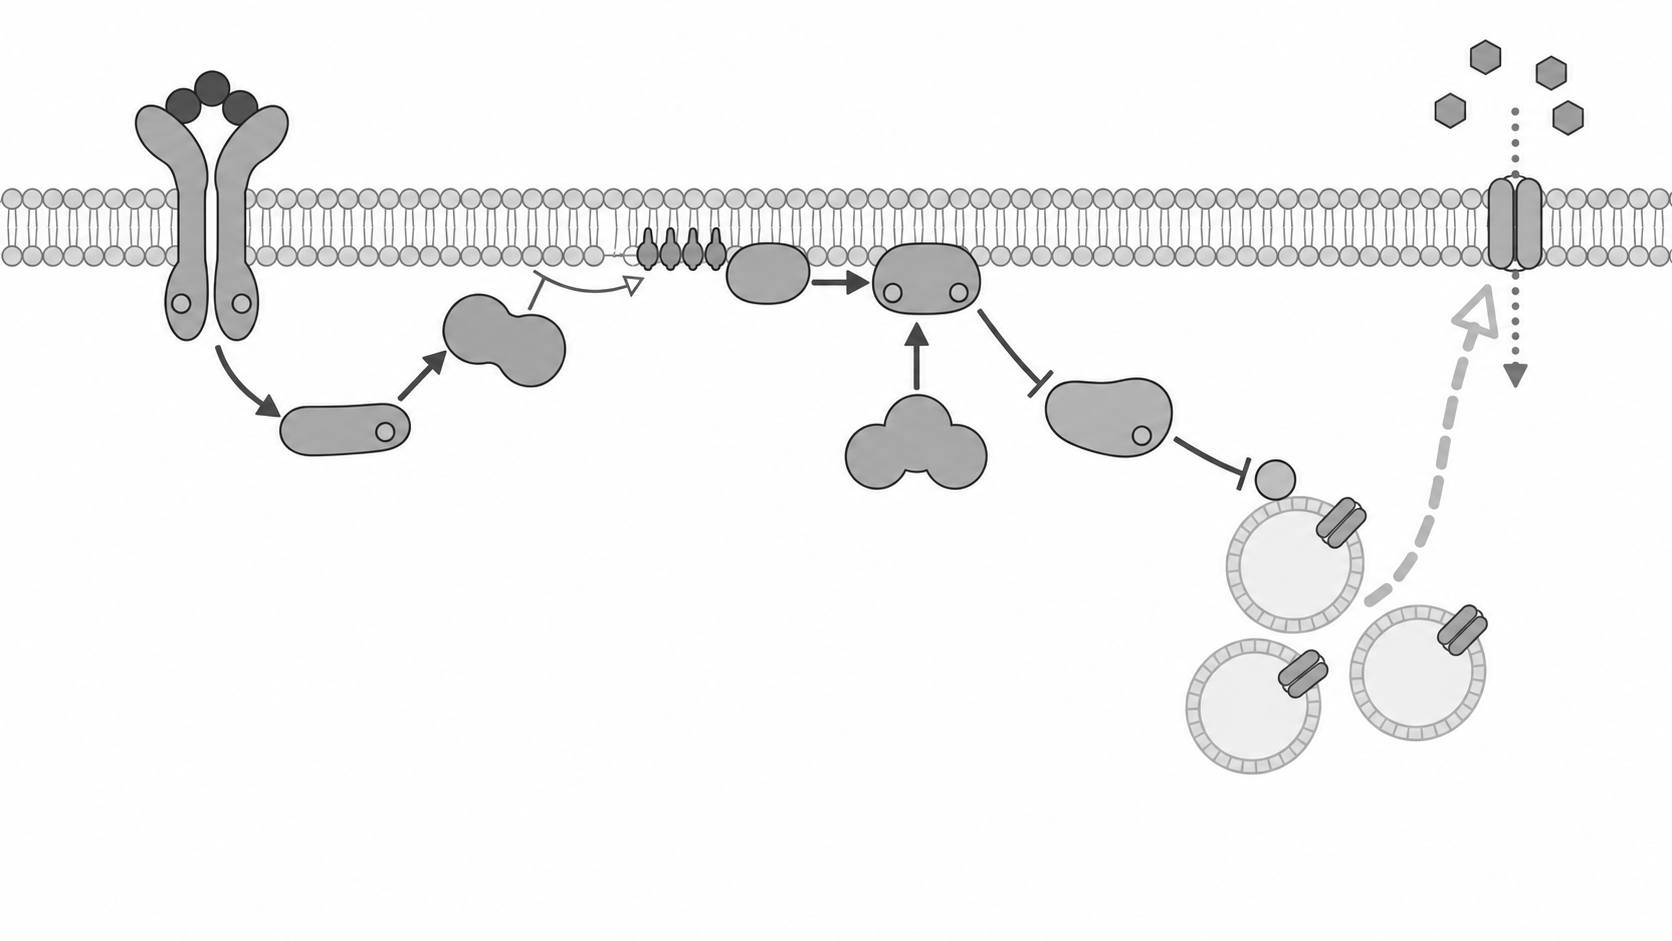
\includegraphics[width=\linewidth]{figures/ch07/ch07-05b-v3-revised-gray.png}\\[1mm]
{\footnotesize (d) Greyscale conversion of panel (b)}
\end{minipage}
\caption{Colour restraint and greyscale testing in mechanism schematics. (a) A different saturated colour for every protein and a rainbow membrane: colour carries no meaning. (b) The revised draft (V3) uses three hues plus grey, one each for signalling proteins, transport regulators, and the transported substance with its carriers. Bottom row: greyscale versions; the hierarchy and line types of (b) remain readable.}\label{fig:ch07-05}
\end{figure}

Generating Figure~\ref{fig:ch07-05}a also underscored model instability: when we first requested a different saturated colour per protein and a rainbow membrane without a reference image, the model rewrote the pathway into a single linear six-protein activation chain, dropping both T-bars and mTORC2 and reversing the glucose arrow! Using Figure~\ref{fig:ch07-05}b as a reference image on the second run preserved the layout, though the $\text{PIP}_2 \rightarrow \text{PIP}_3$ arc arrowhead still switched from hollow to filled.

Comparing Figures~\ref{fig:ch07-05}a and~\ref{fig:ch07-05}b illustrates three principles (Rougier et al., 2014; Wong, 2011): first, colour should encode functional roles rather than individual proteins---Figure~\ref{fig:ch07-05}a scatters red, lime, cyan, magenta, navy, and yellow across proteins without grouping (mTORC2 and Rab share navy despite no link), whereas Figure~\ref{fig:ch07-05}b uses just three hues: medium blue for positive signaling proteins, desaturated grey-blue for negative/trafficking regulators (AS160, Rab), and soft orange for cargo and carriers (glucose, GLUT4, vesicles), plus warm grey for the membrane. Second, avoid pairing red and green (Figure~\ref{fig:ch07-05}a), which is inaccessible to readers with red--green colour-vision deficiency (Wong, 2011; see ColorBrewer 2.0). Third, test in greyscale: in Figure~\ref{fig:ch07-05}c the rainbow membrane turns heavy and protein luminance is chaotic, whereas in Figure~\ref{fig:ch07-05}d functional groups keep uniform luminance and all five line types remain distinct by geometry (while showing that the pale-orange dashed translocation arrow turns light in greyscale, prompting an added text label in the final overlay). You can run \scidraw{}'s Figure Checker (\sdtool{figure-checker}) to flag greyscale and colour-vision risks, remembering that it performs technical checks rather than scientific review.

\section{The Worked Case: From Revision to Final}

We now walk through the closed-loop workflow from the V2 draft (Figure~\ref{fig:ch07-03}b) to the V3 revision (Figure~\ref{fig:ch07-05}b), the V4 final figure (Figure~\ref{fig:ch07-06}), the figure legend, and the verification log.

\subsection{From V2 to V3: Targeted Revision and Catching Unintended Drift}

Checking V2 (Figure~\ref{fig:ch07-03}b) against Table~\ref{tab:ch07-01} confirms correct backbone topology and object counts, but 200\% inspection shows five remaining issues: (1) the $\text{PIP}_2 \rightarrow \text{PIP}_3$ conversion arc (R5) has a closed hollow triangle head rather than an open V, and the PI3K stub meets its left start rather than its midpoint; (2) in membrane recruitment (R6), Akt sits somewhat far from the $\text{PIP}_3$ head groups; (3) narrow white gaps remain at the T-bar ends (R9, R10) and between the translocation arrow tip and membrane GLUT4 (R12); (4) protein fills retain slight shading gradients; and (5) label whitespace is tight in places, while the canvas width corresponds to ~244 ppi at 174 mm print width, below the 300 ppi journal standard.

Our revision instruction from V2 to V3 states what must stay fixed before listing verifiable changes:

\begin{Prompt}
Keep all objects, spatial compartments, and all 13 relations unchanged, and make only
the following modifications:
1. Unify all six signaling proteins (receptor, IRS-1, PI3K, PDK1, Akt, mTORC2) to the
   same flat medium-blue fill and dark-grey outline; unify AS160 and Rab to the same
   desaturated grey-blue fill.
2. Standardize all activation arrows and inhibition lines to a uniform stroke weight,
   with perpendicular T-bar ends touching their target outlines directly.
3. Make the PIP2 -> PIP3 conversion arc thinner in mid-grey with an open V arrowhead,
   and connect the short stub from PI3K to the midpoint of the arc.
4. Keep insulin beads and glucose hexagons at roughly one-third the size of a protein,
   with the three-vesicle GSV cluster clearly visible.
5. Leave at least one protein-width of clear whitespace around every object, keep the
   bottom 12% completely empty, and include no text or symbols anywhere.
\end{Prompt}

Two attempts at generating V3 highlight the danger of \textbf{unintended changes}. First, regenerating from the full V3 prompt without a reference image caused the model to lose all phosphorylation dots, reduce insulin to two beads detached from the receptor, pull PDK1 and Akt off the membrane, invent an unauthorized PI3K $\rightarrow$ PDK1 activation arrow, and draw multiple GLUT4 barrels per vesicle! Second, attaching V2 as a reference image alongside the revision prompt (yielding Figure~\ref{fig:ch07-05}b) preserved all thirteen objects, six phosphorylation dots, membrane contact, and five line styles without extra arrows, though subtle shading, the left-shifted PI3K stub, and tiny T-bar gaps improved only slightly. Thus, \textbf{every revision must be followed by a full-table re-audit, never a spot check of the edited region alone.}

\subsection{V4 Final Artwork: Text-Free Base Image Plus LaTeX/TikZ Overlay}

Why deliver the final figure as a text-free base image plus a LaTeX/TikZ overlay? Image models cannot be trusted to spell molecular names (turning \texttt{Akt} into \texttt{Act} is a factual error), control point sizes, or keep layout fixed across edits. Placing typography in TikZ lets us copy names directly from the verified table, fix print font sizes at 7--8 pt, and share one raster base across English and Chinese editions by swapping only the overlay file. Delivery can follow \textbf{Option A} (base image includes objects and arrows, TikZ adds labels and legend; used here) or \textbf{Option B} (base image has only objects/layers, TikZ draws both arrows and labels; used in the battery case next).

Using V3 as a reference for the V4 base image, the prompt locked the hex palette and reserved empty label rectangles (full prompt in \texttt{cases/}):

\begin{Prompt}
Final base artwork for a journal Figure 1, flat 2D vector-style scientific
schematic, landscape 16:9, print resolution 300 ppi at 174 mm width, pure white
background, uniform thin dark gray (#3A3A3A) outlines, flat fills, no gradients.
THIS IMAGE MUST CONTAIN NO TEXT AT ALL: no letters, words, numbers, or "P".
PALETTE: signaling proteins #A9C4E0 / #4C78A8; insulin #2F5D8C; AS160 and Rab
#B8C2CC; GLUT4 and vesicles #F2C49B / #E39B5B; glucose #C46A2A; membrane
#D9D6D0 / #BDB8AF; phosphorylation dots #E3B23C; lines #3A3A3A and #7A7A7A.
LAYOUT & RELATIONS: keep the same 13 objects, phosphorylation dots, and 5 line
types as the reference image. Leave generous empty white margins above the
membrane, around each protein, and across the bottom 12% strip for overlaid
labels and the figure legend.
\end{Prompt}

Generating V4 again required catching drift and adjusting in layout: an unreferenced first run drew the vesicle GLUT4 barrels inside the vesicle lumens; conditioning on V3 restored proper membrane embedding, and 200\% inspection of the third run confirmed zero stray text or watermarks. Because object edges still intruded into several reserved label boxes, the PI3K stub still joined the left end of the conversion arc, tiny gaps remained at the T-bars, and resolution stayed at ~244 ppi at 174 mm width, we used a normalized $(0,0)$--$(1,1)$ TikZ coordinate system over the base image to fine-tune the seventeen label positions with short leader lines and typeset a vector legend along the bottom band (Figure~\ref{fig:ch07-06}).

\begin{figure}[htbp]\centering
% FIG ch07-06 GLUT4 final overlay (English)
\definecolor{ch07comp}{HTML}{6B6B6B}
\definecolor{ch07transnote}{HTML}{C46A2A}
\definecolor{ch07act}{HTML}{3A3A3A}
\definecolor{ch07conv}{HTML}{7A7A7A}
\definecolor{ch07trans}{HTML}{E39B5B}
\definecolor{ch07flux}{HTML}{C46A2A}
\definecolor{ch07phos}{HTML}{E3B23C}
\begin{tikzpicture}
  \node[anchor=south west, inner sep=0] (img) at (0,0)
    {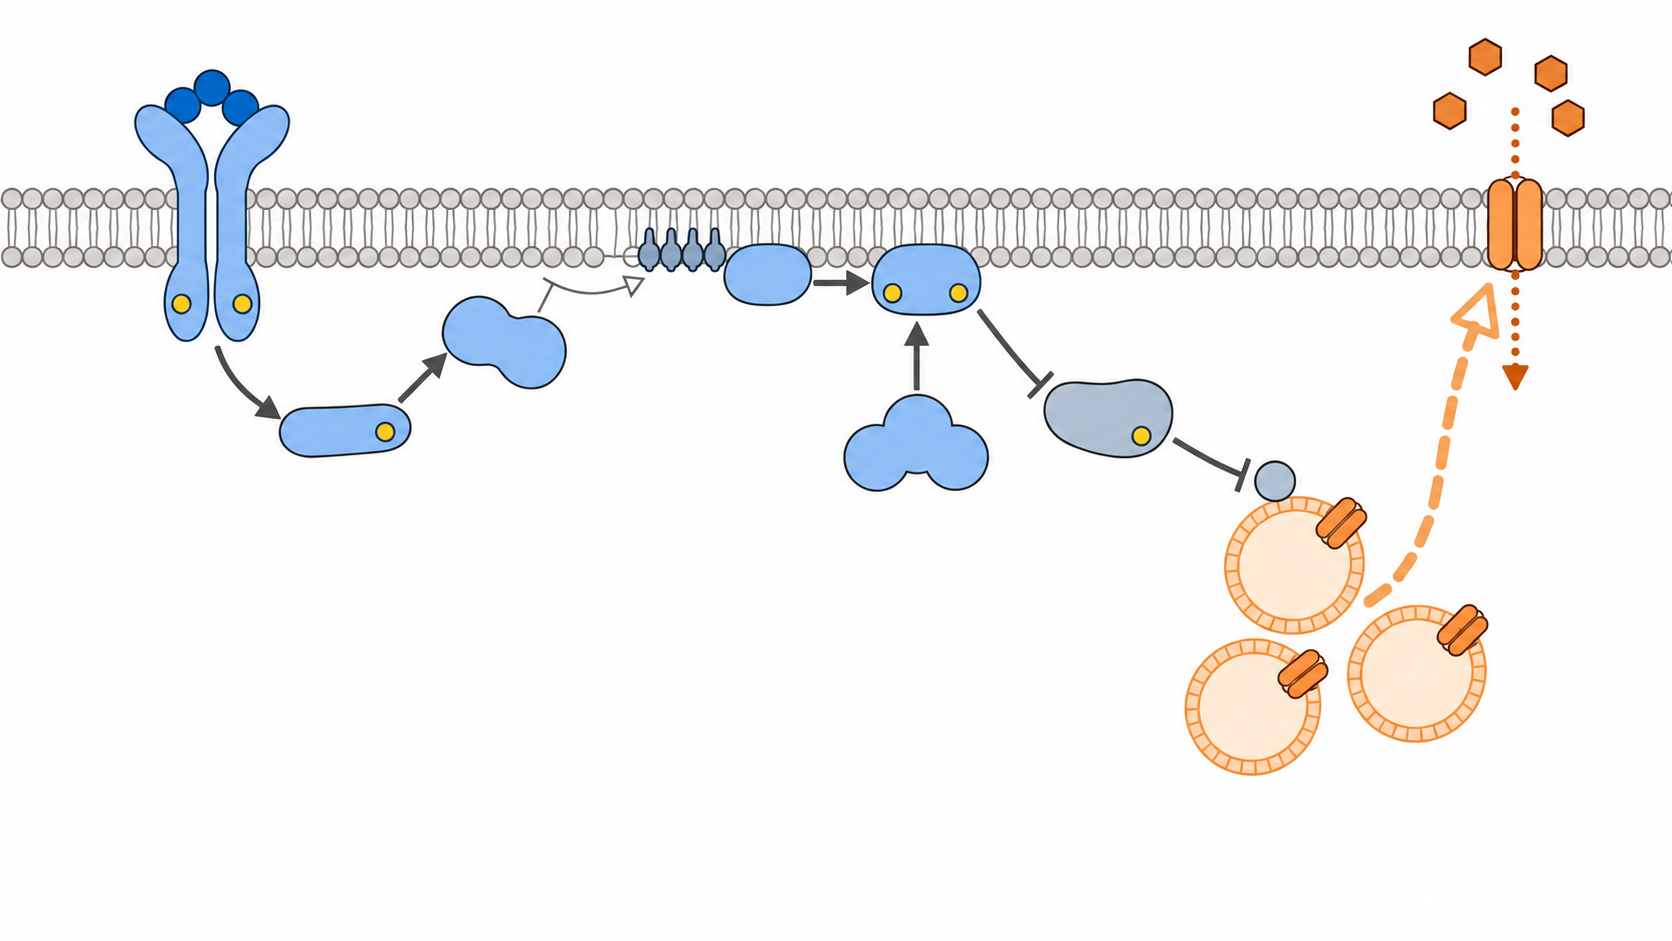
\includegraphics[width=\linewidth]{figures/ch07/ch07-06-v4-base.png}};
  \begin{scope}[x={(img.south east)}, y={(img.north west)},
    font=\sffamily\small]
    \node[text=ch07comp, font=\sffamily\footnotesize\itshape, anchor=west]
      at (0.04, 1-0.055) {Extracellular};
    \node[text=ch07comp, font=\sffamily\footnotesize\itshape]
      at (0.62, 1-0.15) {Plasma membrane};
    \node[text=ch07comp, font=\sffamily\footnotesize\itshape, anchor=west]
      at (0.04, 1-0.90) {Cytoplasm};
    \node[anchor=west, font=\sffamily\small] at (0.20, 1-0.06) {Insulin};
    \draw[BookInk!40, thin] (0.20, 1-0.065) -- (0.145, 1-0.10);
    \node[anchor=west, font=\sffamily\small] at (0.20, 1-0.145) {Insulin receptor};
    \draw[BookInk!40, thin] (0.20, 1-0.15) -- (0.16, 1-0.20);
    \node[font=\sffamily\small] at (0.21, 1-0.56) {IRS-1};
    \node[font=\sffamily\small] at (0.34, 1-0.50) {PI3K};
    \node[font=\sffamily\footnotesize] at (0.48, 1-0.075) {PIP\textsubscript{2} → PIP\textsubscript{3}};
    \draw[BookInk!40, thin] (0.44, 1-0.10) -- (0.385, 1-0.275);
    \node[font=\sffamily\small] at (0.46, 1-0.40) {PDK1};
    \node[font=\sffamily\small] at (0.515, 1-0.375) {Akt};
    \draw[BookInk!40, thin] (0.53, 1-0.36) -- (0.55, 1-0.335);
    \node[font=\sffamily\small] at (0.52, 1-0.60) {mTORC2};
    \draw[BookInk!40, thin] (0.54, 1-0.56) -- (0.55, 1-0.52);
    \node[align=center, font=\sffamily\footnotesize] at (0.80, 1-0.345) {AS160\\(TBC1D4)};
    \draw[BookInk!40, thin] (0.755, 1-0.385) -- (0.695, 1-0.42);
    % Two short lines in the white gap right of the Rab circle (x 0.78–0.84).
    \node[align=left, font=\sffamily\scriptsize, anchor=south west] at (0.788, 1-0.508) {Rab-\\GTP};
    \draw[BookInk!40, thin] (0.784, 1-0.500) -- (0.770, 1-0.512);
    \node[align=center, font=\sffamily\small, anchor=north] at (0.78, 1-0.85) {GLUT4 storage\\vesicles};
    \draw[BookInk!40, thin] (0.78, 1-0.845) -- (0.78, 1-0.80);
    \node[font=\sffamily\small, anchor=west] at (0.94, 1-0.345) {GLUT4};
    \draw[BookInk!40, thin] (0.94, 1-0.33) -- (0.915, 1-0.26);
    \node[font=\sffamily\small, anchor=east] at (0.845, 1-0.065) {Glucose};
    \draw[BookInk!40, thin] (0.845, 1-0.075) -- (0.875, 1-0.09);
    % Right-aligned beside the dashed arrow; the long line stays right of x=0.87.
    \node[text=ch07transnote, font=\sffamily\scriptsize\itshape, align=right, anchor=north east]
      at (0.998, 1-0.430) {translocation\\\& fusion};
    \draw[ch07transnote!55, thin] (0.878, 1-0.448) -- (0.858, 1-0.432);
  \end{scope}
  \node[anchor=north west, font=\sffamily\scriptsize, align=left] at (img.south west) {%
    \begin{tabular}{@{}l@{\quad}l@{}}
      \tikz{\draw[-{Stealth[length=1.5mm]}, ch07act, line width=0.6pt] (0,0) -- (0.22,0);} Activation &
      \tikz{\draw[-{Bar[width=4pt]}, ch07act, line width=0.6pt] (0,0) -- (0.22,0);} Inhibition \\
      \tikz{\draw[ch07conv, line width=0.4pt] (0,0) .. controls (0.08,0.04) .. (0.18,0);} Enz.\ conv. &
      \tikz{\draw[ch07trans, line width=1pt, dashed] (0,0) -- (0.18,0);} Translocation \\
      \tikz{\draw[ch07flux, line width=0.6pt, dotted, -{Stealth[length=1.2mm]}] (0,0) -- (0.18,0);} Glucose flux &
      \tikz{\fill[ch07phos] (0.09,0) circle (1.2pt);} Phosphorylation
    \end{tabular}};
\end{tikzpicture}

\caption{Final schematic of the canonical insulin pathway leading to GLUT4 translocation. The text-free base image was generated by an image model; labels and legend are typeset in LaTeX on top. Solid lines with filled heads, activation; T-bars, inhibition; thin arc, enzymatic conversion; thick dashed arrow, vesicle translocation; dotted arrow, glucose flux; amber dots, phosphorylation. The MAPK and CAP--Cbl--TC10 branches, GLUT4 endocytosis and recycling, negative feedback, SNARE fusion machinery and cytoskeletal transport are omitted; Akt and Rab isoforms are not distinguished, and upstream regulation of mTORC2 is not shown. Based on Saltiel and Kahn (2001), Leto and Saltiel (2012) and Klip et al.\ (2019). The full caption is given in the text.}\label{fig:ch07-06}
\end{figure}

\subsection{Full Figure Legend, Self-Check, and Verification Log}

If you draft a caption with \scidraw{}'s Figure Legend assistant (\sdtool{figure-legend}), use it only as a rough outline and never let it fabricate sample sizes or statistical tests. The complete caption reads:

\begin{BookNote}
\textbf{Figure 1 | Schematic of the canonical insulin signaling pathway leading to GLUT4 translocation.} Insulin binding to the insulin receptor at the plasma membrane triggers tyrosine autophosphorylation of the receptor's intracellular domain, which phosphorylates IRS-1 and recruits class IA PI3K. PI3K converts $\text{PIP}_2$ to $\text{PIP}_3$ in the inner leaflet; $\text{PIP}_3$ recruits PDK1 and Akt, and Akt is activated by phosphorylation by PDK1 and mTORC2. Active Akt phosphorylates AS160 (TBC1D4), inhibiting its Rab-GAP activity. Rab proteins on GLUT4 storage vesicles therefore remain GTP-bound, promoting vesicle translocation to and fusion with the plasma membrane. The resulting increase in surface GLUT4 allows facilitated diffusion of glucose into the cell. Solid lines with filled heads, activation; T-bars, inhibition; thin arc, enzymatic conversion; thick dashed arrow, vesicle translocation; dotted arrow, glucose flux; amber dots, phosphorylation. For clarity, the MAPK and CAP--Cbl--TC10 branches, GLUT4 endocytosis and recycling, negative feedback, the SNARE fusion machinery and cytoskeletal transport are omitted; Rab and Akt isoforms are not distinguished, the parallel role of TBC1D1 in skeletal muscle is not shown, and upstream regulation of mTORC2 is not depicted. Based on reviews by Saltiel and Kahn (2001), Leto and Saltiel (2012) and Klip et al.\ (2019).
\end{BookNote}

A sentence-by-sentence check confirms that the opening sentences map sequentially to R1--R4, R5--R8, and R9--R13; the next sentence defines all six legend symbols; the following sentence states all omissions; and the final sentence cites the literature, with no data or statistical terms. Table~\ref{tab:ch07-verify} excerpts the V4 verification log, separating the author verifier from the domain peer reviewer---neither AI nor technical checks can replace peer review.

\begin{table}[htbp]\centering\scriptsize
\setlength{\tabcolsep}{3pt}
\renewcommand{\arraystretch}{1.1}
\caption{Excerpt from the verification log for the GLUT4 V4 base artwork. Author verifier: first author; domain peer reviewer: metabolism co-author (pending sign-off).}\label{tab:ch07-verify}
\begin{tabularx}{\linewidth}{lYYYY}
\toprule
\textbf{Audit item} & \textbf{Brief specification} & \textbf{Observed V4 result} & \textbf{Status} & \textbf{Disposition} \\
\midrule
R1--R4, R7--R8, R13 & Ligand contact, phosphorylation dots, 4 activation lines, no mTORC2 upstream line, dotted membrane flux & Counts, directions, amber dots, and line styles match brief & Pass & Keep and overlay TikZ labels \\
R5 enzymatic conversion & $\text{PIP}_2 \rightarrow \text{PIP}_3$ thin arc, open V head, PI3K stub at midpoint & Arc points right, but head is closed hollow triangle and stub joins left end & Partial deviation & Logged for teaching draft; redraw in TikZ for submission \\
R6 membrane recruitment & PDK1, Akt touch inner leaflet at $\text{PIP}_3$, no arrow & Both touch inner leaflet without arrows; Akt slightly far from $\text{PIP}_3$ & Partial deviation & Place label between PI3K and PDK1 to aid reading \\
R9--R10 double inhibition & Akt $\dashv$ AS160 $\dashv$ Rab perpendicular T-bars touching targets & Series T-bars correct, Rab on upper-left vesicle; narrow gap at T-bar tips & Partial deviation & Meaning clear; use Option B if strict contact needed \\
R11--R12 translocation & Thick dashed orange arrow to membrane GLUT4; vesicle GLUT4 in membrane & 3 vesicles each embed 1 GLUT4; small gap at dashed arrow tip & Partial deviation & Add ``translocation \& fusion'' label beside arrow \\
No-text \& resolution & No text at 200\% zoom; 300 ppi at 174 mm width & No text at 200\% zoom; ~244 ppi at 174 mm width & Needs higher ppi & Flag as candidate base; do not upscale to fake ppi \\
Unintended changes & Log unrequested edits across rounds & Unreferenced V3 lost dots and added arrow; unreferenced V4 put GLUT4 in lumen & Intercepted & Restored by using prior verified image as reference \\
\bottomrule
\end{tabularx}
\end{table}

\section{Structure Schematics: Layer Order, Materials, and Direction}

For device and materials schematics (battery cells, photovoltaic stacks, membrane assemblies), verification shifts from logical links to four physical dimensions: \textbf{layer sequence} (which layer touches which), \textbf{material pairing} (which collector pairs with which electrode), \textbf{process direction} (paths of ions and electrons), and \textbf{operating state} (charging vs.\ discharging).

Suppose a master's student studying cathode materials wants a pouch-cell cross-section for her thesis introduction. Submitting a single sentence---\texttt{Draw a lithium-ion battery cross-section showing how it charges}---typically yields scrambled layers or reversed ion arrows. Following electrochemical consensus (Goodenough and Park, 2013; Tarascon and Armand, 2001; Armand and Tarascon, 2008; Xu, 2004; Arora and Zhang, 2004; Nitta et al., 2015), we first define the checklist S1--S8 in Table~\ref{tab:ch07-03}.

\begin{table}[htbp]\centering\scriptsize
\setlength{\tabcolsep}{3pt}
\renewcommand{\arraystretch}{1.1}
\caption{Layer-order and process verification table (S1--S8) for a lithium-ion pouch-cell unit cross-section.}\label{tab:ch07-03}
\begin{tabularx}{\linewidth}{lYYYY}
\toprule
\textbf{ID} & \textbf{Item} & \textbf{Correct specification} & \textbf{Common error} & \textbf{Basis} \\
\midrule
S1 & Layer order (left to right) & Pouch film $\rightarrow$ Cu collector $\rightarrow$ negative (graphite) $\rightarrow$ separator $\rightarrow$ positive (e.g.\ $\text{LiCoO}_2$) $\rightarrow$ Al collector $\rightarrow$ pouch film & Separator placed between electrode and collector; electrodes touch directly & Goodenough and Park, 2013; Arora and Zhang, 2004 \\
S2 & Collector pairing & Negative uses Cu foil; positive uses Al foil & Cu and Al swapped & Nitta et al., 2015; textbook convention \\
S3 & Electrolyte location & Wets pores of both electrodes and separator & Drawn as a separate standalone liquid layer & Xu, 2004 \\
S4 & $\text{Li}^+$ during charging & De-intercalates from positive, crosses separator, intercalates into graphite negative (right $\rightarrow$ left) & Direction reversed (left $\rightarrow$ right) & Goodenough and Park, 2013 \\
S5 & Electrons during charging & Positive $\rightarrow$ external circuit (charger) $\rightarrow$ negative & Electrons cross separator/electrolyte & Same as above \\
S6 & Discharging $\text{Li}^+$ / $\text{e}^-$ & $\text{Li}^+$ negative $\rightarrow$ positive (left $\rightarrow$ right) in electrolyte; $\text{e}^-$ negative $\rightarrow$ load $\rightarrow$ positive & Directions not reversed with state & Same as above \\
S7 & $\text{Li}^+$ path & Migrates only inside cell (in electrolyte) & $\text{Li}^+$ drawn in external wire & Same as above \\
S8 & Nomenclature & Label ``Negative / Positive electrode''; note in caption that anode/cathode follow discharge convention & Labelling anode/cathode on charging plot without note, or swapping them & Textbook convention \\
\bottomrule
\end{tabularx}
\end{table}

We first generated Figure~\ref{fig:ch07-07} from a deliberately error-inducing prompt so readers can spot four common mistakes against Table~\ref{tab:ch07-03}: (1) the left graphite negative electrode is paired with silver-grey Al foil and the right positive electrode with Cu foil (swapped collectors, violating S2); (2) graphite flakes and slate-blue positive oxide particles touch directly (an internal short circuit in a real cell) while the white porous separator sits between the positive electrode and the right Cu foil (violating S1); (3) the panel is labelled ``Charging,'' yet all six orange $\text{Li}^+$ spheres inside the electrodes point right, from negative to positive (violating S4); and (4) three orange $\text{Li}^+$ spheres with arrows travel along the top external wire (violating S7).

\begin{figure}[htbp]\centering
% FIG ch07-07 battery common errors overlay (English)
\definecolor{ch07err}{HTML}{C0392B}
\begin{tikzpicture}
  \node[anchor=south west, inner sep=0] (img) at (0,0)
    {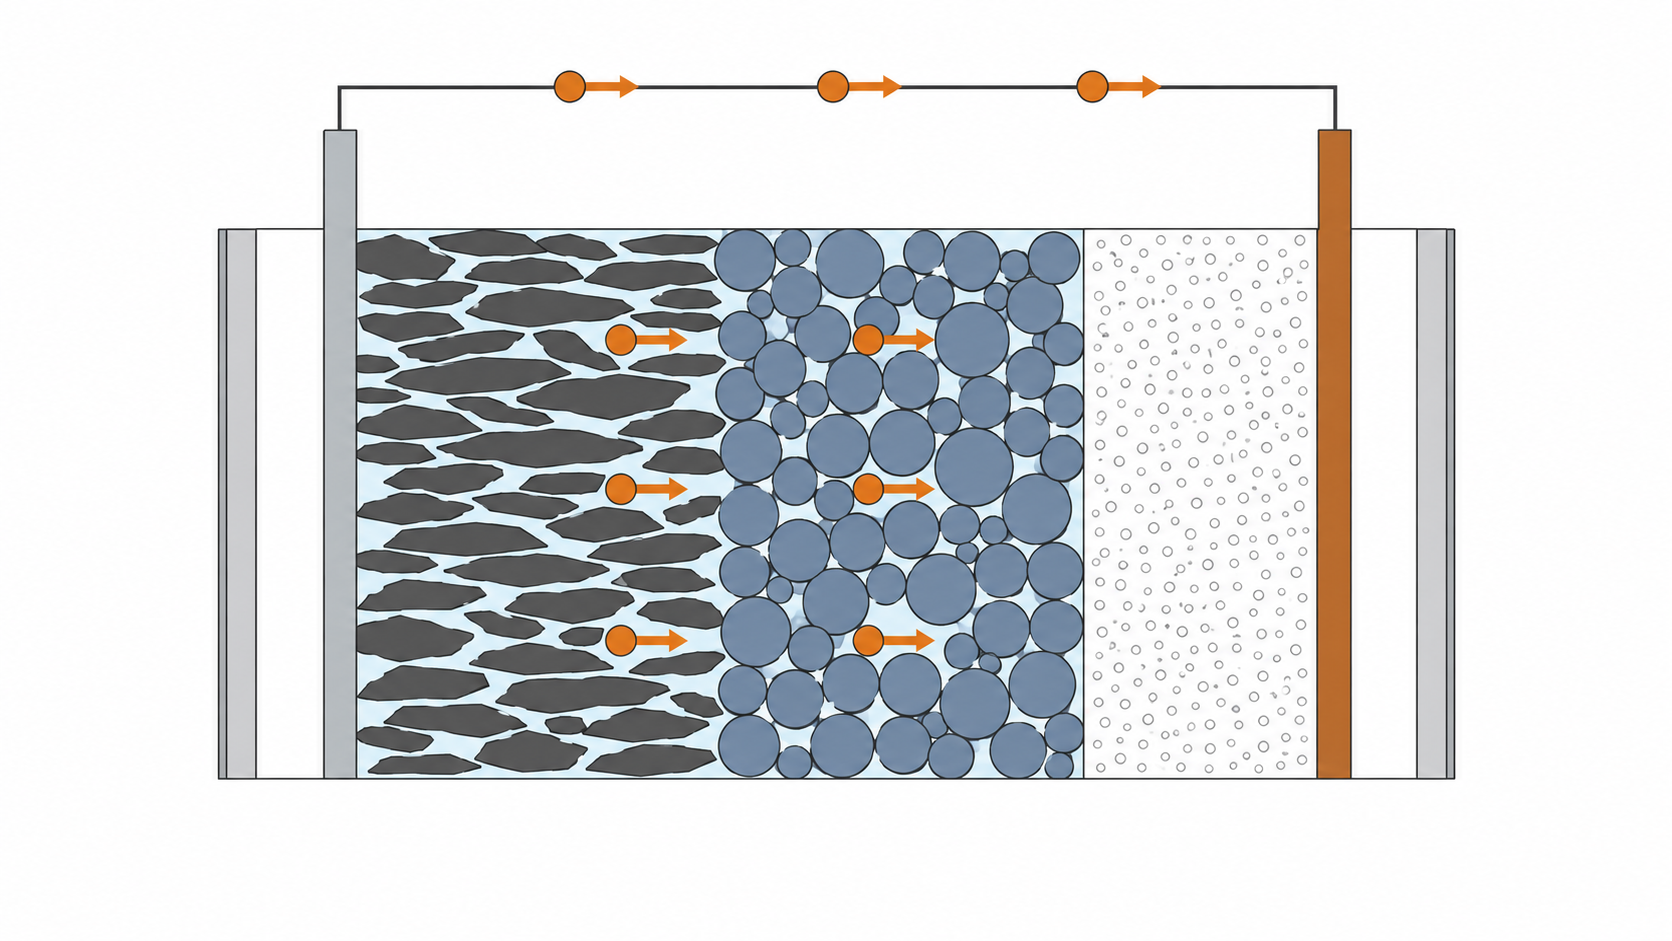
\includegraphics[width=\linewidth]{figures/ch07/ch07-07-battery-errors.png}};
  \begin{scope}[x={(img.south east)}, y={(img.north west)},
    font=\sffamily\small]
    \node[font=\bfseries] at (0.50, 1-0.02) {Charging (incorrect example)};
    \node[font=\scriptsize] at (0.20, 1-0.90) {Al foil};
    \node[font=\scriptsize, align=center] at (0.315, 1-0.90) {Negative\\(graphite)};
    \node[font=\scriptsize, align=center] at (0.525, 1-0.90) {Positive\\(e.g.\ LiCoO$_2$)};
    \node[font=\scriptsize] at (0.69, 1-0.90) {Separator};
    \node[font=\scriptsize] at (0.76, 1-0.94) {Cu foil};
    \node[font=\scriptsize, rotate=90, anchor=south] at (0.15, 1-0.20) {Pouch};
    \node[font=\scriptsize] at (0.20, 1-0.11) {Negative tab};
    \node[font=\scriptsize] at (0.76, 1-0.11) {Positive tab};
    \node[font=\scriptsize\bfseries, text=white, fill=ch07err, circle, inner sep=1.5pt] at (0.20, 1-0.22) {1};
    \node[font=\scriptsize\bfseries, text=white, fill=ch07err, circle, inner sep=1.5pt] at (0.76, 1-0.22) {1};
    \node[font=\scriptsize\bfseries, text=white, fill=ch07err, circle, inner sep=1.5pt] at (0.42, 1-0.22) {2};
    \node[font=\scriptsize\bfseries, text=white, fill=ch07err, circle, inner sep=1.5pt] at (0.40, 1-0.55) {3};
    \node[font=\scriptsize\bfseries, text=white, fill=ch07err, circle, inner sep=1.5pt] at (0.50, 1-0.08) {4};
    \node[font=\scriptsize, text=BookInk!80, anchor=north] at (0.50, 1-0.96)
      {1--4 map to checklist S2, S1, S4, S7 in Table~7-3};
  \end{scope}
\end{tikzpicture}

\caption{A deliberately incorrect battery schematic, generated by an image model from a prompt that specified the errors. (1) The copper and aluminium current collectors are swapped. (2) The separator is not between the electrodes, so the electrodes touch, which in a real cell means an internal short circuit. (3) The panel is labelled as charging, yet Li$^+$ moves from the negative to the positive electrode. (4) Li$^+$ is drawn travelling through the external circuit. See Figure~\ref{fig:ch07-08} for the correct version.}\label{fig:ch07-07}
\end{figure}

Why does the correct figure (Figure~\ref{fig:ch07-08}) exclude arrows from the AI base image? Because arrow direction is the core scientific content and reverses between charging and discharging; generating two separate images would cause random drift in layer widths and particle packing, implying that the cell structure changes between states. We therefore generate the structure-only base image once and overlay both sets of process arrows in TikZ:

\begin{Prompt}
[Purpose & Audience] Introductory structure schematic (double-column width 174 mm, two
panels side by side) for materials science and electrochemistry readers.
[Goal] Show the exact layer sequence and collector pairing of a single repeating unit of
a lithium-ion pouch cell, and contrast the internal Li+ and external electron paths
between charging and discharging.
[Objects & Counts] Each structural layer appears once from left to right: outer pouch
film, copper current collector with top tab, graphite negative electrode coating,
porous separator, layered-oxide positive electrode coating (e.g., LiCoO2), aluminium
current collector with top tab, outer pouch film; pale-blue electrolyte filling pores.
[Process Overlay (in TikZ only, absent from base image)]
(a) Charging: Li+ from positive -> separator -> negative; e- from positive tab -> charger -> negative tab.
(b) Discharging: Li+ from negative -> separator -> positive; e- from negative tab -> load -> positive tab.
Li+ stays strictly inside the electrolyte; electrons stay strictly in the external wire.
[Layout & Visuals] 16:9 cross-section; vertical layer bands across x 0.14-0.86; top and
bottom margins empty for external circuit and legend. Flat 2D vector style on white.
[Restrictions] Base image contains NO text, symbols, +/- signs, ions, electrons, arrows,
or wires; omit SEI layer, binder, conductive carbon, and packaging seals; not to scale.
\end{Prompt}

Across three runs of this base prompt, the first run added two unwanted pale-blue vertical bands between the pouch films and collectors that looked like standalone liquid layers (violating S3), and the third left the separator pores white with sparse positive particles. The second run cleanly produced the sequence ``pouch film--Cu collector--flaky graphite negative--central porous separator--spherical oxide positive--Al collector--pouch film'' with no ions, wires, or text (zooming in shows only slight unevenness in the pale-blue separator pores). In LaTeX, we called this single base image twice side by side and overlaid the top external circuit (charger or load), dashed electron arrows ($\text{e}^-$), and solid orange internal $\text{Li}^+$ arrows in TikZ (Figure~\ref{fig:ch07-08}). Note that converting a bitmap to PPTX or SVG only separates text from background rather than turning particles or separators into semantically editable objects, so directional arrows belong in TikZ or vector software.

\begin{figure}[htbp]\centering
% FIG ch07-08 charge/discharge overlay (English)
\definecolor{ch07Li}{HTML}{D9822B}
\definecolor{ch07wire}{HTML}{3A3A3A}
\definecolor{ch07elec}{HTML}{3A3A3A}
\definecolor{ch07electrolyte}{HTML}{E3F0F8}
\begin{tikzpicture}
  \node[anchor=south west, inner sep=0] (imgA) at (0,0)
    {\includegraphics[width=0.49\linewidth]{\chsevenpanelbase}};
  \node[anchor=south west, inner sep=0] (imgB) at (0.51\linewidth,0)
    {\includegraphics[width=0.49\linewidth]{\chsevenpanelbase}};
  \begin{scope}[shift={(imgA.south west)},
    x={($(imgA.south east)-(imgA.south west)$)},
    y={($(imgA.north west)-(imgA.south west)$)},
    font=\sffamily\small]
    \node[anchor=south west, font=\sffamily\small] at (0.00, 1.20) {\textbf{(a)} Charging};
    \node[align=center, font=\sffamily\scriptsize, anchor=north west] at (0.25, 1.045) {Negative\\tab};
    \node[align=center, font=\sffamily\scriptsize, anchor=north east] at (0.75, 1.045) {Positive\\tab};
    \chsevendrawcircuit{Charger}
  \end{scope}
  \begin{scope}[shift={(imgB.south west)},
    x={($(imgB.south east)-(imgB.south west)$)},
    y={($(imgB.north west)-(imgB.south west)$)},
    font=\sffamily\small]
    \node[anchor=south west, font=\sffamily\small] at (0.00, 1.20) {\textbf{(b)} Discharging};
    \chsevendrawcircuitb{Load}
  \end{scope}
  \begin{scope}[shift={(imgA.south west)},
    x={($(imgA.south east)-(imgA.south west)$)},
    y={($(imgA.north west)-(imgA.south west)$)},
    font=\sffamily\scriptsize]
    \node[align=center, anchor=north] at (0.323, 0.19) {Negative\\(graphite)};
    \node[anchor=north] at (0.50, 0.19) {Separator};
    \node[align=center, anchor=north] at (0.678, 0.19) {Positive\\(LiCoO\textsubscript{2})};
    \draw[BookInk!45, thin] (0.193, 0.19) -- (0.193, -0.02);
    \node[align=center, anchor=north] at (0.193, -0.02) {Cu\\collector};
    \draw[BookInk!45, thin] (0.806, 0.19) -- (0.806, -0.02);
    \node[align=center, anchor=north] at (0.806, -0.02) {Al\\collector};
  \end{scope}
  \node[anchor=north, font=\sffamily\scriptsize, align=center] at (0.5\linewidth, -0.13\linewidth) {%
    \begin{tabular}{@{}c@{\qquad}c@{}}
      \tikz{\draw[-{Stealth[length=1.5mm]}, ch07Li, line width=0.7pt] (0,0) -- (0.2,0);} Li\textsuperscript{+} migration (in electrolyte) &
      \tikz{\draw[ch07elec, line width=0.6pt, dashed, -{Stealth[length=1.2mm]}] (0,0) -- (0.2,0);} Electron flow (external circuit) \\[0.4em]
      \multicolumn{2}{c}{\tikz{\fill[ch07electrolyte] (0,0) rectangle (0.08,0.06);} Electrolyte (fills pores)} \\[0.35em]
      \multicolumn{2}{c}{Outer light-grey bars are the pouch}
    \end{tabular}};
\end{tikzpicture}

\caption{Cross-section of one repeating unit of a lithium-ion pouch cell. Both panels use the same structural base image (generated by an image model, with no text or arrows); arrows, external circuit and labels are overlaid in LaTeX. (a) Charging: Li$^+$ leaves the positive electrode, crosses the separator through the electrolyte and intercalates into the graphite negative electrode, while electrons flow through the external circuit from the positive to the negative electrode. (b) Discharging: the directions reverse, and electrons pass through the load from the negative to the positive electrode. The negative electrode sits on a copper current collector and the positive electrode on aluminium; electrolyte fills the pores of both electrodes and the separator. Layers are not to scale (the separator is widened), only one unit is shown (real pouch cells stack or wind many double-coated electrodes), and the SEI, binder, conductive additive and packaging details are omitted. ``Negative'' and ``positive'' electrode correspond to the anode and cathode as named for discharge.}\label{fig:ch07-08}
\end{figure}

\section{What AI Can and Cannot Do, and What the Author Must Verify}

Table~\ref{tab:ch07-02} summarizes the capability boundaries of AI (including \scidraw{}) and what the author must verify at each step.

\begin{table}[htbp]\centering\scriptsize
\setlength{\tabcolsep}{3pt}
\renewcommand{\arraystretch}{1.1}
\caption{What AI can do, what AI cannot do, and what the author must verify when creating mechanism and structure schematics.}\label{tab:ch07-02}
\begin{tabularx}{\linewidth}{lYYY}
\toprule
\textbf{Stage} & \textbf{What AI (including \scidraw{}) can do} & \textbf{What AI cannot do} & \textbf{What the author must verify} \\
\midrule
Structuring relations & Rewrite an author's relation table into prompt clauses; the wizard's ``Mechanism \& workflow diagram'' route lines up the generate, refine, legend, and check tools & Judge whether a relation is established or contested; read a full paper to find the true mechanism & Literature basis per row; established / simplified / hypothesised tags; ``do not draw'' list \\
Sketch \& layout & Combine sketch and text in sketch mode to generate candidates roughly following the layout & Guarantee hard layout locking or object permanence; give identical layouts across runs & Compartments, reading path, object counts, and drift from the sketch \\
Generating base & Produce flat, text-free candidates in the mechanism or prompt generator; batch candidates & Guarantee no extra/missing objects, no pseudo-text, or exact hex values and line weights & Row-by-row audit against R1--R13 or S1--S8; 200\% zoom check for stray glyphs \\
Revising & Select a prior image and apply text revision instructions iteratively & Edit only the specified spot without affecting other regions & Full-table re-verification after each edit; log unintended changes \\
Lines \& colour & Draw specified line styles and palettes; Figure Checker reports greyscale, colour-vision, and ppi metrics & Decide scientific meaning of line styles; technical checks do not replace scientific review & One-to-one legend mapping; colours encode roles only; greyscale legibility \\
Labels \& arrows & None (in this chapter, labels and key process arrows are not delegated to image models) & Reliably spell molecule names or sub/superscripts; flip directions across states without structure drift & Labels copied verbatim from list; arrow directions match operating state \\
Figure legend & Figure Legend assistant drafts an initial caption from the image & Know what was omitted or which papers were cited; add sample sizes or statistics (inappropriate here) & Each sentence maps to relation table; omissions stated; natural prose \\
Delivery & Multi-panel layout and export (Chapter 9) & Image-to-PPTX/SVG does not turn base bitmaps into semantically editable objects & Typeset vector text; sufficient base resolution; peer review \\
\bottomrule
\end{tabularx}
\end{table}

\section{Chapter Checklist}

\begin{itemize}
\item Compile a complete relation table (source, target, interaction class, compartment, evidence status) or layer-order table before writing any image prompt, and append an explicit ``do not draw'' exclusion list.
\item Fix the exact count of every object; whenever an entity legitimately appears twice (such as GLUT4 in intracellular vesicles and in the plasma membrane), state that exception explicitly in the brief.
\item Encode spatial compartments (extracellular space, membrane bilayer, cytoplasm) or structural layer sequences directly in the brief and verify that every boundary is visually distinct.
\item Assign each interaction class to a single, mutually exclusive line style, define every style in the figure legend, and visually separate working hypotheses from established consensus.
\item Eliminate ``shortcut arrows'': preserve essential intermediate nodes in indirect pathways such as double-negative regulatory steps (inhibition of an inhibitor).
\item Restrict colour to encoding functional roles (at most three hues plus neutral grey), avoid simultaneous red--green contrasts, and confirm that all relations remain legible in greyscale.
\item Inspect the base image at 200\% zoom to confirm the absence of baked-in text, pseudo-characters, or unrequested organelles; add all labels in a vector typesetting layer copied verbatim from your verified list.
\item For structural schematics, audit layer sequence, current-collector or substrate pairing, transport paths, and operating state (e.g.\ charging vs.\ discharging) item by item; generate the structural base once and distinguish states via vector overlays.
\item Re-audit the entire verification table after every AI revision rather than checking only the edited spot, and record any unintended drift.
\item Disclose all omitted branches, isoform simplifications, and non-scale dimensions in the figure legend, and ensure no fabricated sample sizes or statistical terms appear.
\item Have at least one domain peer independently review the pathway topology or device layer stack before submission.
\end{itemize}

\section{Exercises}

\begin{enumerate}
\item \textbf{Unpacking a shortcut arrow (pen and paper).} Many introductory slides compress insulin signaling into a single arrow: ``$\text{Akt} \rightarrow \text{GLUT4 translocation}$.'' (a) List the omitted intermediate molecules and assign each link a specific line style from Figure~\ref{fig:ch07-01}. (b) Explain in two sentences why the link between Akt and AS160 must be drawn as an inhibition bar even though the net effect of the pathway is to stimulate translocation. (c) Write out the corresponding three-row relation table (source, target, relation type, line style, literature basis), citing the specific review paper and section you consulted.

\item \textbf{Hands-on with \scidraw{}: one mechanism, two inputs.} Choose an established textbook mechanism from your own field comprising no more than eight objects. (a) Write all ten brief fields (including explicit spatial compartments and a line-style dictionary) in your own document and save it; then open the Scientific Figure Workflow wizard (\sdtool{figure-workflow}), choose ``Mechanism \& workflow diagram'', and follow the route into the mechanism generator. (b) First, open the mechanism generator (\sdtool{mechanism-figure-generator}) and submit a single-sentence prompt; audit the output against a verification table and document at least five specific scientific or visual flaws. (c) Next, submit your full structured brief to generate a text-free base image and compare the two verification tables side by side. (d) Select one generated image, apply a targeted modification instruction, and document at least one ``unintended change'' that occurred outside the targeted region. Submit both images, both verification tables, your revision prompt, and your drift log.

\item \textbf{Spotting and fixing structural errors.} Consider a single-cell cross-section of a proton-exchange membrane fuel cell (PEMFC), or another layered device from your discipline. (a) Write out the left-to-right layer sequence, the material of each layer, and the transport paths and directions of $\text{H}^+$, electrons ($\text{e}^-$), and $\text{H}_2/\text{O}_2/\text{H}_2\text{O}$ during power generation, citing a textbook or review source. (b) Draft an error-inducing prompt designed to plant three common structural or directional mistakes, followed by a clean structure-only base prompt (excluding all arrows, ions, and text). (c) Overlay the operating arrows, external load circuit, and layer labels in TikZ on top of the clean base image, and convert the result to greyscale to verify that all transport paths remain distinct.
\end{enumerate}

\section*{References}

\begin{itemize}
\item Armand M, Tarascon JM. Building better batteries. \emph{Nature}. 2008;451(7179):652--657. doi:10.1038/451652a
\item Arora P, Zhang Z. Battery separators. \emph{Chem Rev}. 2004;104(10):4419--4462. doi:10.1021/cr020738u
\item ColorBrewer 2.0: Color advice for cartography and scientific visualization. \url{https://colorbrewer2.org/}
\item Goodenough JB, Park KS. The Li-ion rechargeable battery: a perspective. \emph{J Am Chem Soc}. 2013;135(4):1167--1176. doi:10.1021/ja3091438
\item Klip A, McGraw TE, James DE. Thirty sweet years of GLUT4. \emph{J Biol Chem}. 2019;294(30):11369--11381. doi:10.1074/jbc.REV119.008351
\item Le Nov\`ere N, Hucka M, Mi H, Moodie S, Schreiber F, Sorokin A, et al. The Systems Biology Graphical Notation. \emph{Nat Biotechnol}. 2009;27(8):735--741. doi:10.1038/nbt.1558
\item Leto D, Saltiel AR. Regulation of glucose transport by insulin: traffic control of GLUT4. \emph{Nat Rev Mol Cell Biol}. 2012;13(6):383--396. doi:10.1038/nrm3351
\item Nitta N, Wu F, Lee JT, Yushin G. Li-ion battery materials: present and future. \emph{Mater Today}. 2015;18(5):252--264. doi:10.1016/j.mattod.2014.10.040
\item Rougier NP, Droettboom M, Bourne PE. Ten simple rules for better figures. \emph{PLoS Comput Biol}. 2014;10(9):e1003833. doi:10.1371/journal.pcbi.1003833
\item Saltiel AR, Kahn CR. Insulin signalling and the regulation of glucose and lipid metabolism. \emph{Nature}. 2001;414(6865):799--806. doi:10.1038/414799a
\item Sano H, Kane S, Sano E, M\^{\i}inea CP, Asara JM, Lane WS, Garner CW, Lienhard GE. Insulin-stimulated phosphorylation of a Rab GTPase-activating protein regulates GLUT4 translocation. \emph{J Biol Chem}. 2003;278(17):14599--14602. doi:10.1074/jbc.C300063200
\item Sarbassov DD, Guertin DA, Ali SM, Sabatini DM. Phosphorylation and regulation of Akt/PKB by the Rictor-mTOR complex. \emph{Science}. 2005;307(5712):1098--1101. doi:10.1126/science.1106148
\item Systems Biology Graphical Notation (SBGN) official website. \url{https://sbgn.github.io/}
\item Tarascon JM, Armand M. Issues and challenges facing rechargeable lithium batteries. \emph{Nature}. 2001;414(6861):359--367. doi:10.1038/35104644
\item Wong B. Points of view: Color blindness. \emph{Nat Methods}. 2011;8(6):441. doi:10.1038/nmeth.1618
\item Xu K. Nonaqueous liquid electrolytes for lithium-based rechargeable batteries. \emph{Chem Rev}. 2004;104(10):4303--4418. doi:10.1021/cr030203g
\end{itemize}

\chapter{Presenting Experimental Images Honestly}

Su, a graduate student in cell biology, was preparing a manuscript on a high-content phenotypic screen of small-molecule compounds. For the supplementary methods section, she needed a figure illustrating the baseline staining quality of nuclei and mitochondria in human osteosarcoma cells (U2OS) from a dimethyl sulfoxide (DMSO) vehicle-control well. She copied several micrographs off the imaging workstation, dragged them into a slide presentation program, and pulled the brightness and contrast sliders until the dim mitochondrial panel ``looked clear.'' She then took a screen capture of the slide and uploaded the screenshot to a generative image tool with the prompt: ``Denoise, sharpen, and upscale to high resolution.''

At lab meeting, her advisor did not comment on how crisp the panels looked. Instead, she asked three questions. First, where are the unmodified 16-bit raw files stored? Second, which exact intervals of raw greyscale values were mapped to black and white in the nuclear and mitochondrial channels, and were the control fields displayed with the exact same intensity window? Third, from which objective magnification and camera pixel size was that ``$20\ \mu\text{m}$'' scale bar in the lower right corner calculated? Su could not answer any of the three. Taking a screenshot had permanently crushed the 16-bit measurements into 8-bit RGB values; the slide sliders left no numerical record of the transfer function; and the scale bar had been drawn by eye to resemble a figure from another paper.

Experimental images differ fundamentally from the workflow diagrams of Chapter~6 and the mechanism schematics of Chapter~7: \textbf{an experimental image is a measurement, not an illustration.} Whether the file comes from a fluorescence microscope, a scanning electron microscope (SEM), a Western blot imager, or a pathology scanner, the numerical value stored at each pixel records the photon or electron count registered by a detector at a defined spatial coordinate. When preparing evidentiary images for publication, AI tools serve only three supporting roles: helping organize a presentation plan, drafting deterministic scripts that read raw arrays and assemble panels without altering source files, and running technical checks on exported figures for file format, resolution, and colour-vision accessibility. \textbf{Generative AI must never touch the pixel values of an evidentiary image.} Using two classes of openly licensed raw micrographs---multichannel fluorescence images of cultured cells and SEM images of plant leaf epidermis---this chapter walks through raw-file stewardship, intensity display mapping, pseudo-colour selection, cropping, scale-bar calibration, journal image-integrity policies, and verifiable delivery logs.

\section{Raw Images Are Evidence: Data, Display, and Export}

In every digital imaging system, \textbf{raw data, display settings, and exported images} are three distinct entities. Confusing what appears on a monitor with what is stored in the file is the root cause of most accidental image distortion and compliance failures.

When a scientific camera---such as an sCMOS or CCD detector---captures a fluorescence micrograph, photons striking each photosite are converted into photoelectrons and quantized by an analogue-to-digital converter (ADC) into integer grey levels. Depending on the hardware, each pixel is digitized at 12 bits ($0\text{--}4095$), 14 bits ($0\text{--}16383$), or 16 bits ($0\text{--}65535$) and saved inside an uncompressed TIFF container or native instrument format (such as OME-TIFF, ND2, CZI, or LIF) paired with acquisition metadata. That two-dimensional integer matrix is the primary measurement.

Standard monitors, web browsers, and PDF viewers, however, display only 8 bits per colour channel ($256$ grey levels, from $0$ to $255$). To render a 16-bit array on an 8-bit screen, viewing software must execute a \textbf{display mapping}: it chooses a lower bound (the black point, $v_{\min}$) and an upper bound (the white point, $v_{\max}$), renders every pixel with $I \le v_{\min}$ as pure black ($0$), renders every pixel with $I \ge v_{\max}$ as pure white ($255$), and scales intermediate values across $[0, 255]$. Under a linear display mapping, the 8-bit displayed grey level $I_{\text{disp}}$ for a raw pixel value $I$ is
\[
I_{\text{disp}} = \operatorname{clip}\!\left(\frac{I - v_{\min}}{v_{\max} - v_{\min}},\, 0,\, 1\right) \times 255.
\]
So long as the source file is not overwritten, changing $v_{\min}$ and $v_{\max}$ only shifts the viewing window; the integer matrix inside the TIFF file remains untouched. Once a researcher clicks ``Save As 8-bit PNG/JPEG'' or takes a screenshot, however, the display mapping is baked irreversibly into the pixel values: measurements outside $[v_{\min}, v_{\max}]$ are permanently clipped, and the 12- or 16-bit dynamic range is collapsed into $256$ discrete steps.

We illustrate this distinction using primary micrographs from the Broad Bioimage Benchmark Collection dataset BBBC022v1 (Gustafsdottir et al., 2013; Ljosa et al., 2012; dedicated to the public domain under CC0~1.0 by Anne Carpenter). Our fluorescence material comes from plate 20585, well A13 (a DMSO vehicle-control well marked \texttt{mock} in the metadata), site~1 (\texttt{s1}) and site~2 (\texttt{s2}), comprising two single-channel files per site: channel \texttt{w1} records Hoechst~33342 nuclear staining, and channel \texttt{w5} records MitoTracker Deep Red mitochondrial staining. Each file is a $696 \times 520$-pixel 16-bit greyscale TIFF acquired with a $20\times$ objective at $0.656\ \mu\text{m/pixel}$, using a camera with an effective 12-bit ADC depth (ceiling $4095$).

In the raw array of the site~1 nuclear channel (\texttt{w1}), all $361,920$ pixels span $121\text{--}1655$, with a mean of $238.4$, $0.1\text{th}$ and $99.9\text{th}$ percentiles of $132$ and $1236$, and zero pixels at the camera ceiling of $4095$. Figure~\ref{fig:ch08-01} renders this single 16-bit array under three linear display windows alongside the corresponding raw-value histograms.

\begin{figure}[htbp]\centering
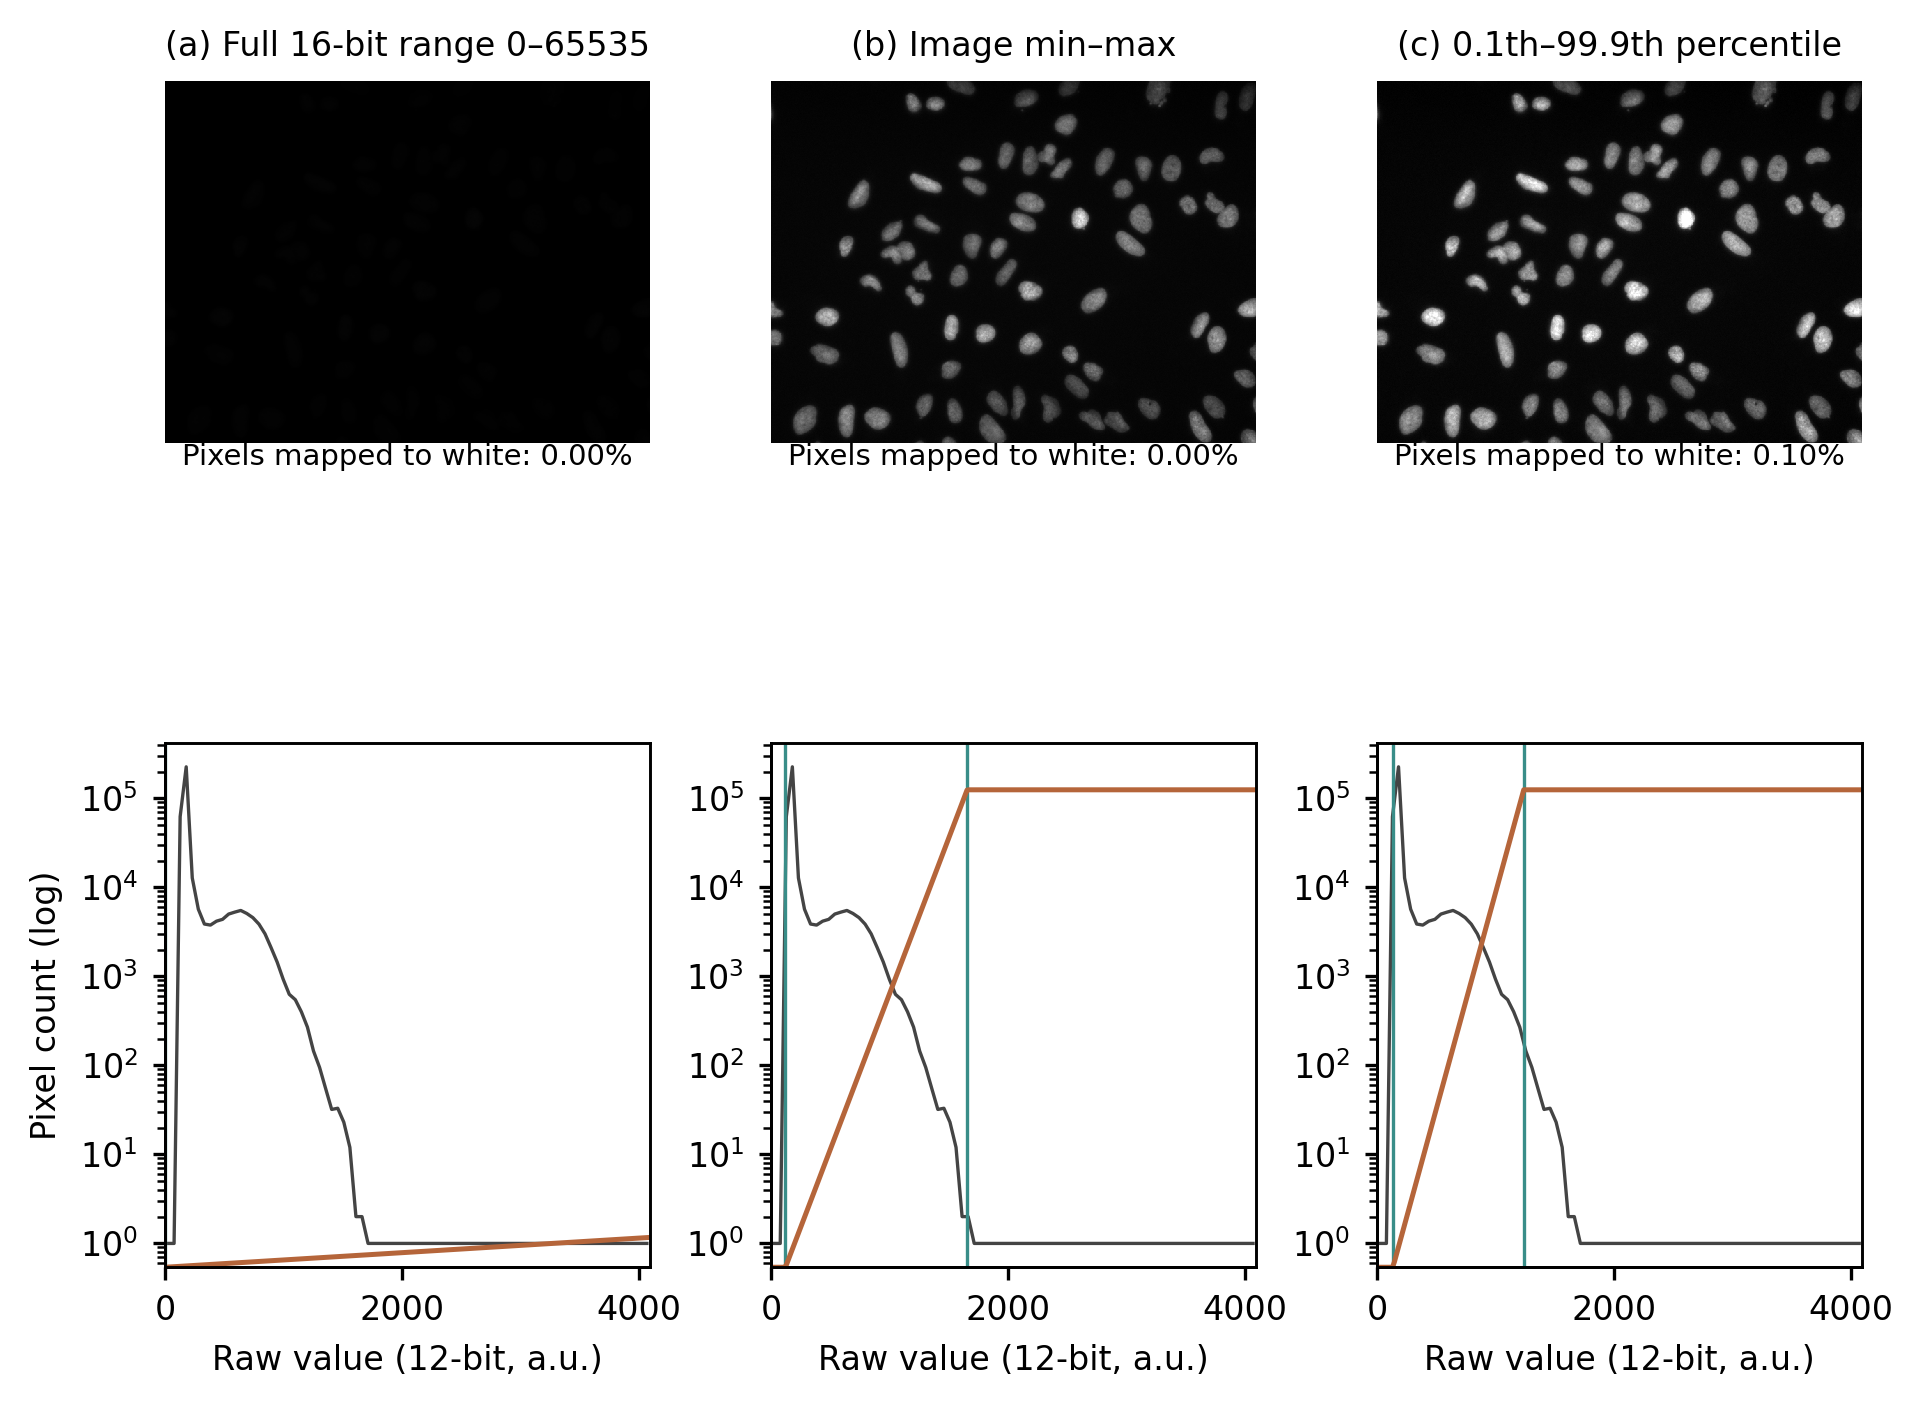
\includegraphics[width=0.88\linewidth]{figures/ch08/ch08-01-raw-display-mapping-en.png}
\caption{One 16-bit fluorescence image (BBBC022, Hoechst channel) shown with three linear display mappings. Raw pixel values are identical in all columns; only the mapping changes: (a) full 16-bit range; (b) image minimum to maximum; (c) $0.1\text{th}$ to $99.9\text{th}$ percentile, with the fraction of pixels mapped to white stated. Bottom: histograms of raw values with the mapping overlaid. Image: BBBC022v1, CC0.}\label{fig:ch08-01}
\end{figure}

Comparing the three columns of Figure~\ref{fig:ch08-01} shows how display mapping governs visual appearance:
\begin{itemize}
\item \textbf{Column (a) (linear mapping across the full 16-bit container range, $0\text{--}65535$):} Generic operating-system viewers map $0$ to black and $65535$ to white when opening a 16-bit TIFF. Because a 12-bit camera never exceeds $4095$ and this field peaks at $1655$, even the brightest pixel maps to $1655 / 65535 \times 255 \approx 6.4$. The top-left panel therefore appears pitch black ($0.00\%$ of pixels mapped to white), and the brown transfer line in the bottom-left plot hugs the horizontal axis. Beginners often mistake this dark window for a failed exposure and overwrite the original file in a photo editor.
\item \textbf{Column (b) (linear mapping from image minimum to maximum, $121\text{--}1655$):} Setting $v_{\min} = 121$ and $v_{\max} = 1655$ (between the two vertical teal lines in the middle histogram) raises the slope of the transfer line, revealing all roughly $60$ nuclei with $0.00\%$ of pixels mapped to white. However, a single condensed, intensely bright nucleus above and to the right of centre pushes the global maximum to $1655$, leaving the remaining interphase nuclei relatively dim.
\item \textbf{Column (c) (linear mapping from the $0.1\text{th}$ to the $99.9\text{th}$ percentile, $132\text{--}1236$):} Setting $v_{\min} = 132$ and $v_{\max} = 1236$ clips only the brightest $0.10\%$ of pixels (concentrated inside that single condensed nucleus) to pure white, spreading the 8-bit greyscale across the interphase population so chromatin texture is clearly resolved.
\end{itemize}

Authors must distinguish two very different kinds of ``pixel ceiling.'' The first is \textbf{display-stage clipping}, as in Figure~\ref{fig:ch08-01}c, where raw values above $1236$ map to $255$ on screen while $1655$ remains intact inside the 16-bit TIFF. The second is \textbf{acquisition-stage sensor saturation} inside the camera ADC. In the site~1 mitochondrial channel (\texttt{w5}), raw pixel values span $185\text{--}4095$ (mean $373.2$, $p_{0.1}/p_{99.9} = 218/1140$), and \textbf{$12$ pixels equal the 12-bit ADC ceiling of $4095$}. Those $12$ pixels overflowed during exposure; no post-processing algorithm can recover their true photon counts. For qualitative methods panels with a few isolated saturated pixels, the honest course is to leave the pixels unaltered and report the count in the catalogue and legend; if saturation affects regions used for intensity quantification, the sample must be re-imaged at shorter exposure.

The first rule of experimental image stewardship follows: \textbf{copy before processing, and lock raw files as read-only.} Store original files in a write-protected directory, compute SHA-256 checksums, and compile a \textbf{raw-image catalogue} recording filename, hash, bit depth, dimensions, physical pixel size, and acquisition metadata. All display mapping and cropping should then run via a deterministic script that reads the read-only masters and writes lossless 8-bit PNG or TIFF display derivatives---never using lossy JPEGs or screenshots as source files. General-purpose AI assistants can write Python scripts to scan directories, compute SHA-256 digests, and count saturated pixels; the author must verify the camera's effective bit depth ($4095$ versus $65535$) and confirm the source of the physical pixel size.

\section{Contrast Adjustments: Linear, Non-Linear, and Disclosed}

Editorial policies at major journals---including the \emph{Journal of Cell Biology} (Rossner and Yamada, 2004) and Nature Portfolio---define four boundaries for contrast adjustments.

\textbf{First, whole-image linear adjustments are permitted, provided they do not obscure or eliminate valid data.} Within $[v_{\min}, v_{\max}]$, subtracting the black point preserves the exact intensity ratio between any two nonsaturated features. Pushing $v_{\min}$ above background to make the background look ``clean,'' or pulling $v_{\max}$ down to make dim features blaze, clips real signal into $0$ or $255$ and erases structural detail.

\textbf{Second, non-linear transfer functions---such as gamma ($\gamma$) correction, logarithmic transforms, or spline curves---alter relative intensity ratios across the dynamic range and must be disclosed in the figure legend.} Under a gamma mapping,
\[
I_{\text{disp}} = \left[\operatorname{clip}\!\left(\frac{I - v_{\min}}{v_{\max} - v_{\min}},\, 0,\, 1\right)\right]^{\gamma} \times 255.
\]
When $\gamma < 1$ (e.g., $\gamma = 0.5$), the transfer curve bows upward, boosting weak signals while compressing bright signals so structures that differ several-fold in raw photon counts appear similar in brightness.

Figure~\ref{fig:ch08-02} quantifies this effect on the site~1 mitochondrial channel (\texttt{w5}) across a linear mapping, a $\gamma = 0.5$ mapping with the same black and white points, and an over-clipped linear counter-example. We fix two $15 \times 15$-pixel regions of interest (ROIs): a bright perinuclear mitochondrial cluster at $(340, 210)\text{--}(355, 225)$ (cyan tick) and a dim peripheral cytoplasmic region at $(120, 380)\text{--}(135, 395)$ (yellow tick). After subtracting the black point ($218$), the ratio of mean raw intensities between the bright and dim ROIs is $3.57$.

\begin{figure}[htbp]\centering
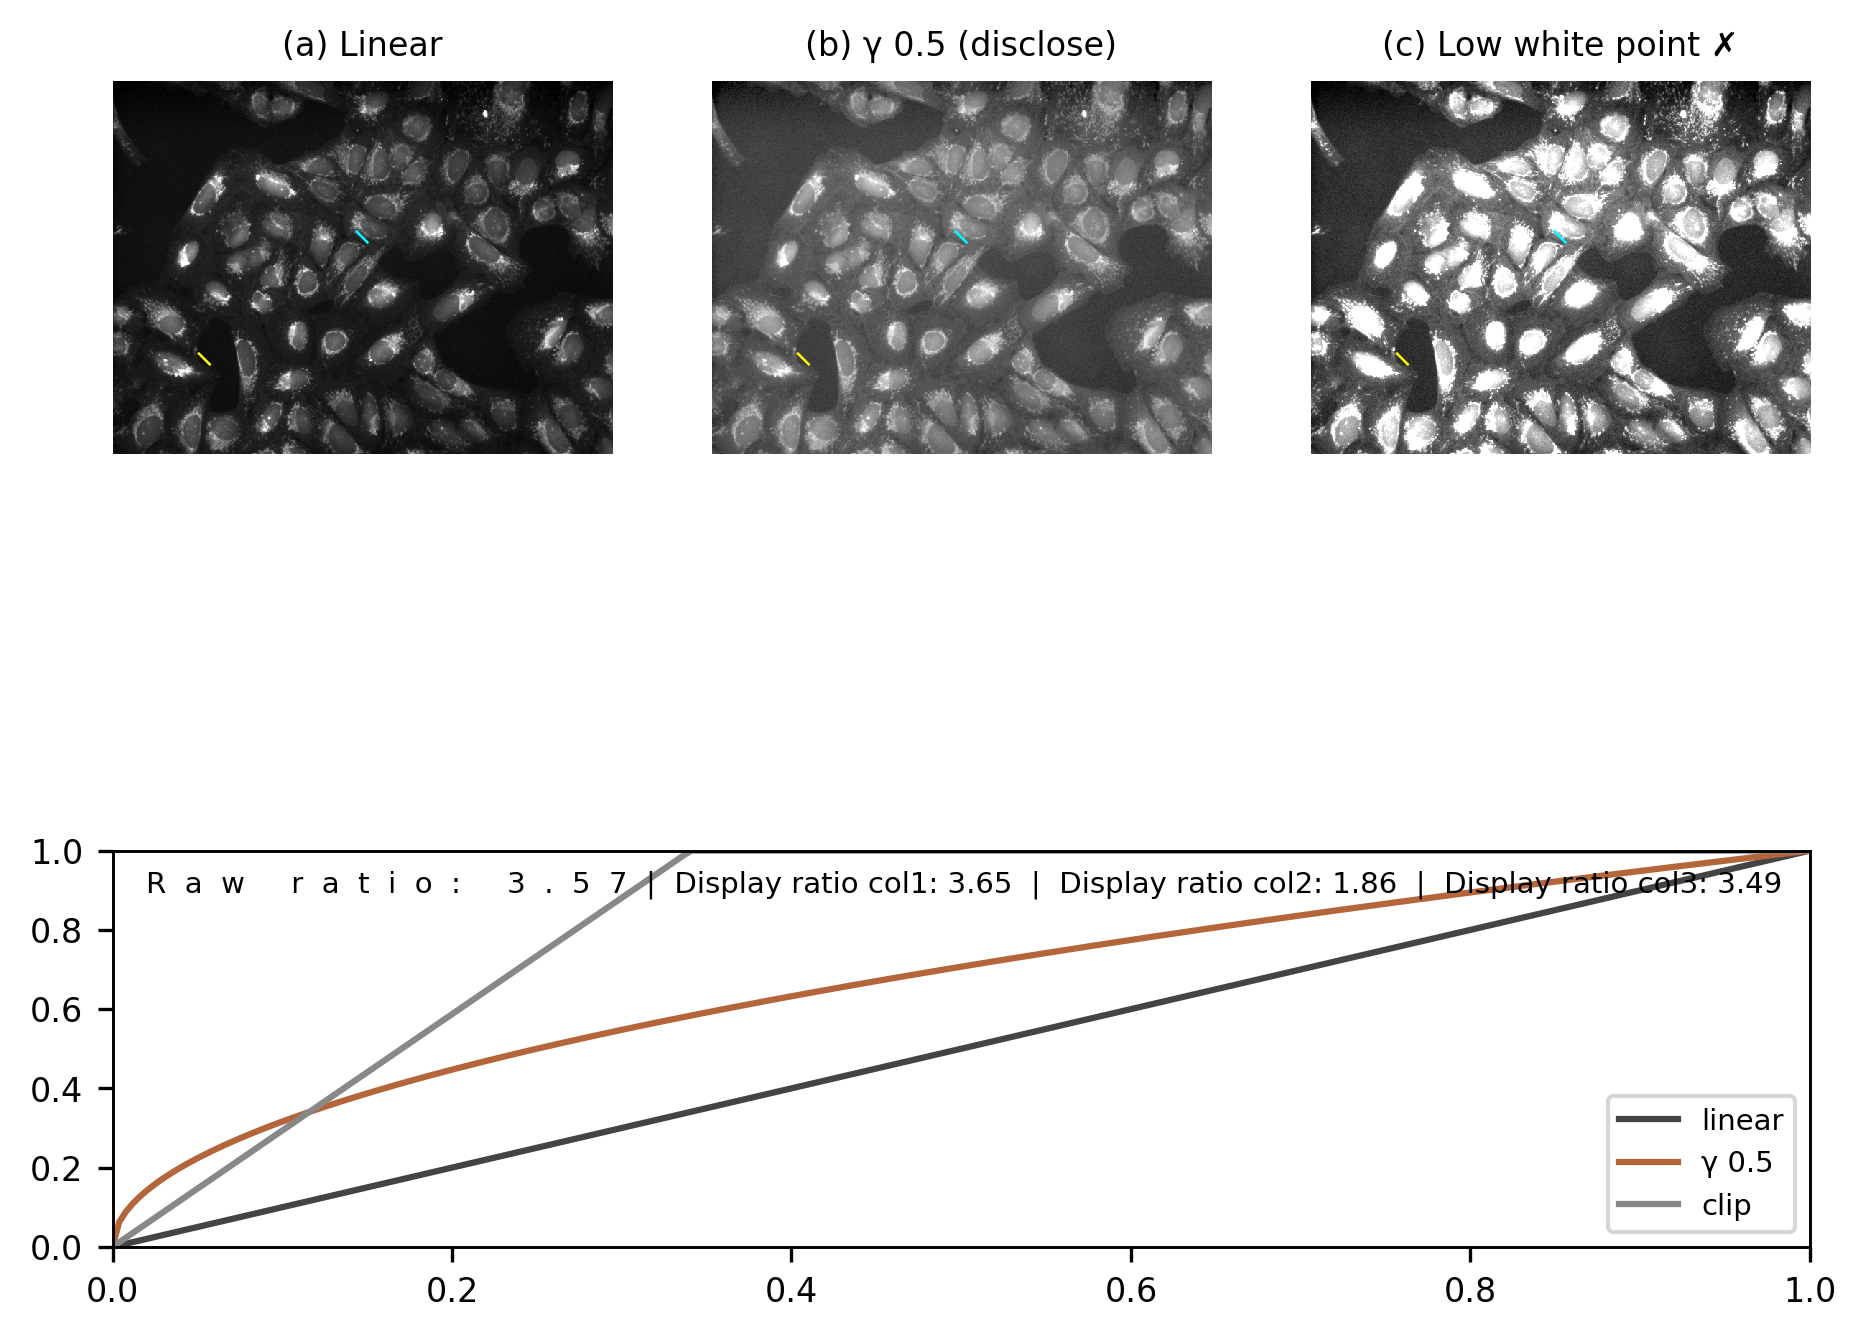
\includegraphics[width=0.88\linewidth]{figures/ch08/ch08-02-linear-vs-gamma-en.png}
\caption{Linear versus non-linear display. (a) Linear mapping ($218\text{--}1140$). (b) The same image with $\gamma = 0.5$: dim signal is brightened and the relative intensity of bright and dim regions changes, so the adjustment must be disclosed. (c) Counter-example: a white point set too low clips most mitochondrial signal to white and destroys information. Curves show the three mappings and list the raw intensity ratio and display grey-level ratios for two fixed regions (cyan and yellow ticks). Image: BBBC022v1, CC0.}\label{fig:ch08-02}
\end{figure}

Inspecting the three columns and transfer curves in Figure~\ref{fig:ch08-02} shows why disclosure is mandatory:
\begin{enumerate}
\item \textbf{Panel (a) (linear mapping, $218\text{--}1140$):} Perinuclear clusters and distal cytoplasmic tubules are resolved in true proportion; the 8-bit displayed grey-level ratio between the cyan and yellow ROIs is $3.65$ (\texttt{Display ratio col1: 3.65}), matching the raw ratio of $3.57$ within integer rounding.
\item \textbf{Panel (b) ($\gamma = 0.5$ over $218\text{--}1140$):} The brown curve arches upward, brightening peripheral tubules, but the displayed ROI ratio drops from $3.57$ to $1.86$ (\texttt{Display ratio col2: 1.86})---nearly halving the apparent contrast. Without disclosing $\gamma = 0.5$ in the legend, readers misjudge the spatial distribution of signal.
\item \textbf{Panel (c) (counter-example: white point lowered to the $90\text{th}$ percentile, $532$):} The grey line hits the ceiling about one-third of the way across the horizontal axis, clipping \textbf{$9.94\%$ of all pixels to pure white ($255$)}. Although the ROI mean ratio numerically reads $3.49$ (\texttt{Display ratio col3: 3.49}, because the steeper slope inflates the dim ROI while clamping the bright ROI at $255$), perinuclear mitochondria collapse into solid white blobs with all internal morphology lost.
\end{enumerate}

\textbf{Third, thresholding backgrounds to zero, local dodging or burning, and clone-stamp or healing-brush retouching are strictly forbidden.} Selectively brightening cells or painting over fluorescent debris falsifies empirical data (Rossner and Yamada, 2004; Cromey, 2010).

\textbf{Fourth, all panels compared within a figure must share identical display settings.} Applying per-panel ``auto-contrast'' cancels out real treatment differences and manufactures fake differences between identical controls. Figure~\ref{fig:ch08-03} demonstrates this using two adjacent fields (\texttt{s1} and \texttt{s2}, mitochondrial channel) from the \emph{same} DMSO control well (well A13). As shown in the right-hand bar chart, the whole-field mean raw intensities of the two 16-bit arrays are nearly identical: $373.2\ \text{a.u.}$ for \texttt{s1} and $366.3\ \text{a.u.}$ for \texttt{s2}, differing by less than $2\%$ (each bar is a single field mean shown to verify baseline magnitude, not a statistical test).

\begin{figure}[htbp]\centering
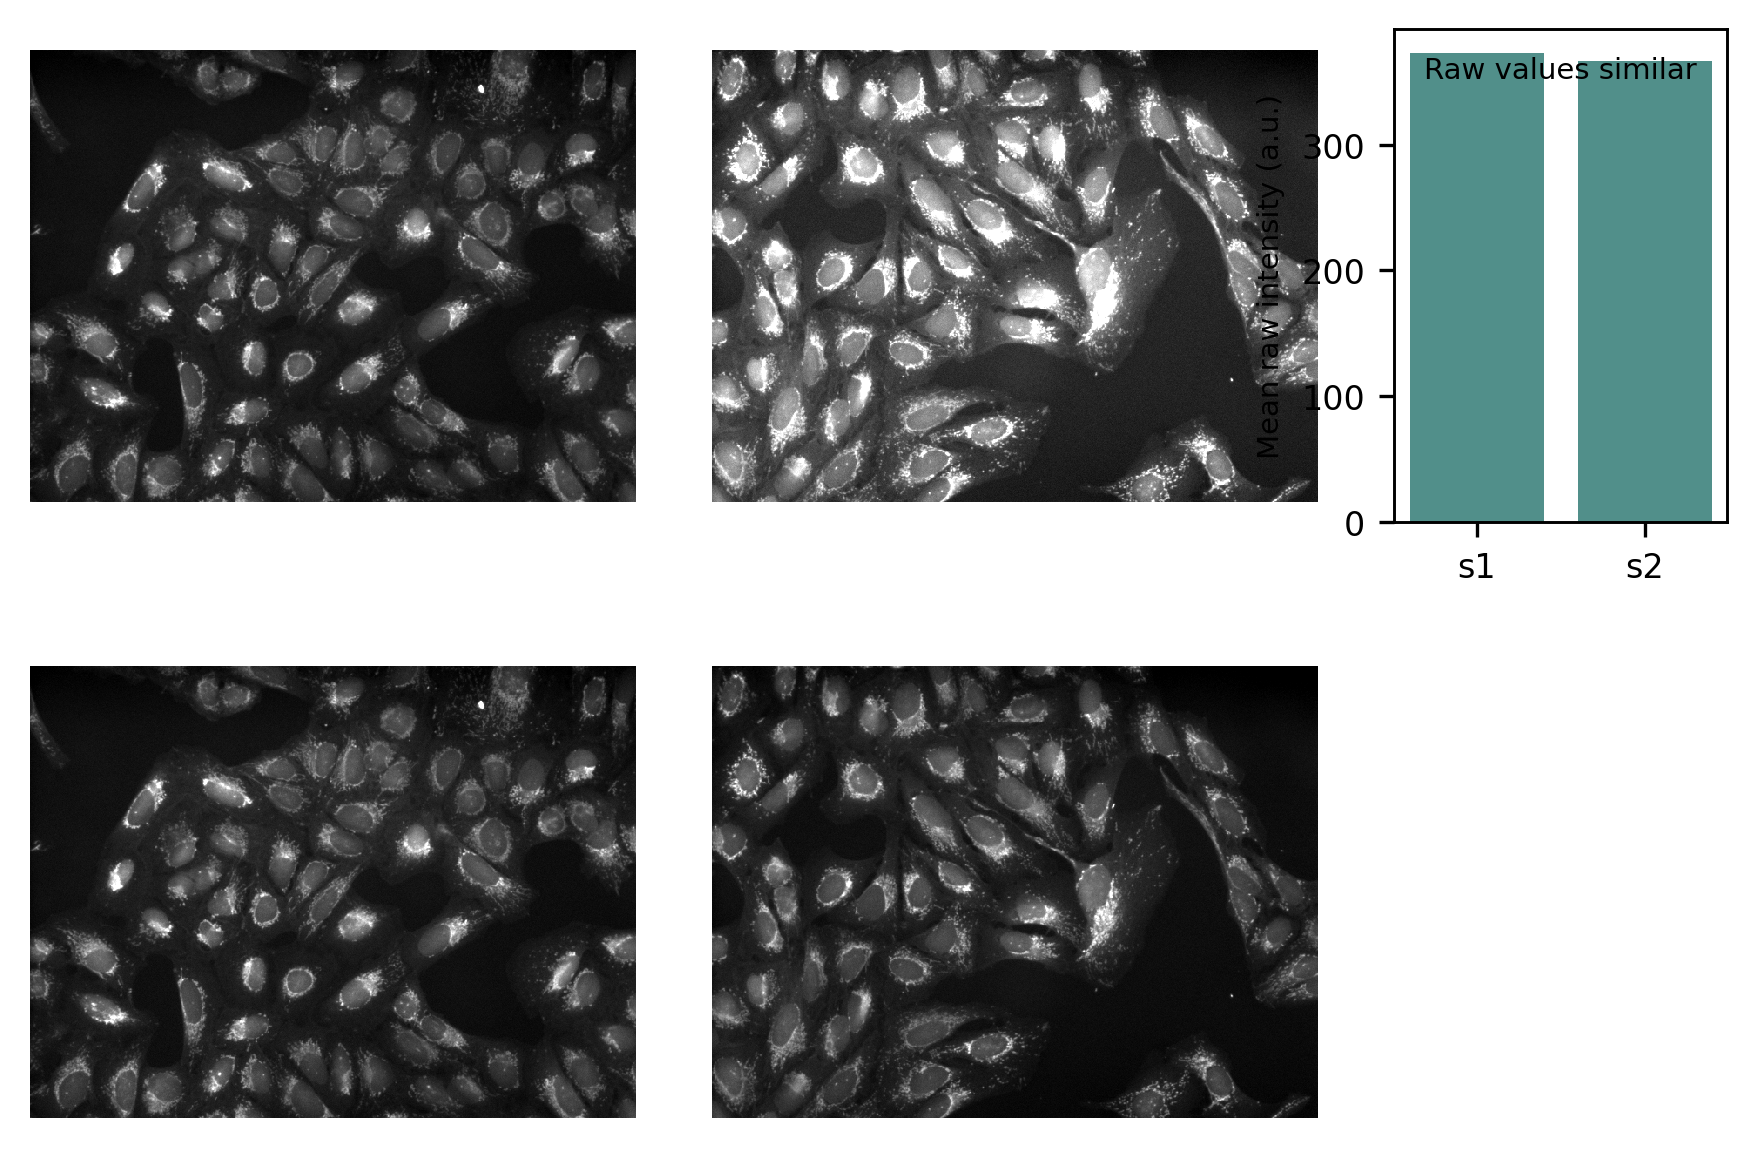
\includegraphics[width=0.88\linewidth]{figures/ch08/ch08-03-consistent-display-en.png}
\caption{Compared panels must share display settings. Both images come from the same control well (BBBC022, well A13, sites~1 and~2) with no treatment difference. Top: display ranges set separately, so the right image appears brighter. Bottom: one shared range ($218\text{--}1140$), and the apparent difference disappears. Right: mean raw intensity of the two fields. The top-right display range was chosen deliberately as a counter-example. Image: BBBC022v1, CC0.}\label{fig:ch08-03}
\end{figure}

In the top row of Figure~\ref{fig:ch08-03}, \texttt{s1} is mapped over $218\text{--}1140$ while \texttt{s2} has its white point lowered to $196\text{--}700$. Lowering the white point by $39\%$ makes the right panel blaze with bright mitochondria, mimicking a strong treatment effect; in the bottom row, applying the shared range $218\text{--}1140$ restores visual parity.

\section{Channels and Pseudo-Colour}

Monochrome fluorescence cameras capture each emission band as a single-channel greyscale array; the colours seen in figures are lookup tables (LUTs) chosen by the author. Selecting channel LUTs follows three rules.

\textbf{First, avoid red/green merges; use magenta/green (or cyan/magenta/yellow) and provide split-channel greyscale panels.} Roughly $8\%$ of male readers have red--green colour-vision deficiency (Wong, 2011; Crameri et al., 2020). In a red/green overlay, pure red ($R$) and pure green ($G$) project onto similar yellow-brown hues under deuteranopia or protanopia, making the two channels and yellow ($R+G$) colocalization regions hard to tell apart. Mapping the first channel to \textbf{magenta} (writing identical 8-bit grey values into both red $R$ and blue $B$) and the second to \textbf{green} ($G$) adds a strong short-wavelength blue component, and overlapping signal sums to high-contrast white ($R+G+B$), remaining separable under both deuteranopia and protanopia. Moreover, human vision resolves fine spatial detail better in single-channel greyscale than in colour (Schmied and Jambor, 2020; Jambor et al., 2021), making ``split-channel greyscale + magenta/green merge'' the safest combination.

Figure~\ref{fig:ch08-04} tests both palettes on a $300 \times 300$-pixel crop from site~1 ($(198, 110)\text{--}(498, 410)$, with display windows fixed at $132\text{--}1236$ for nuclei and $218\text{--}1140$ for mitochondria), simulating colour-vision deficiency in linear sRGB space with the model of Machado et al.\ (2009) at severity $1.0$.

\begin{figure}[htbp]\centering
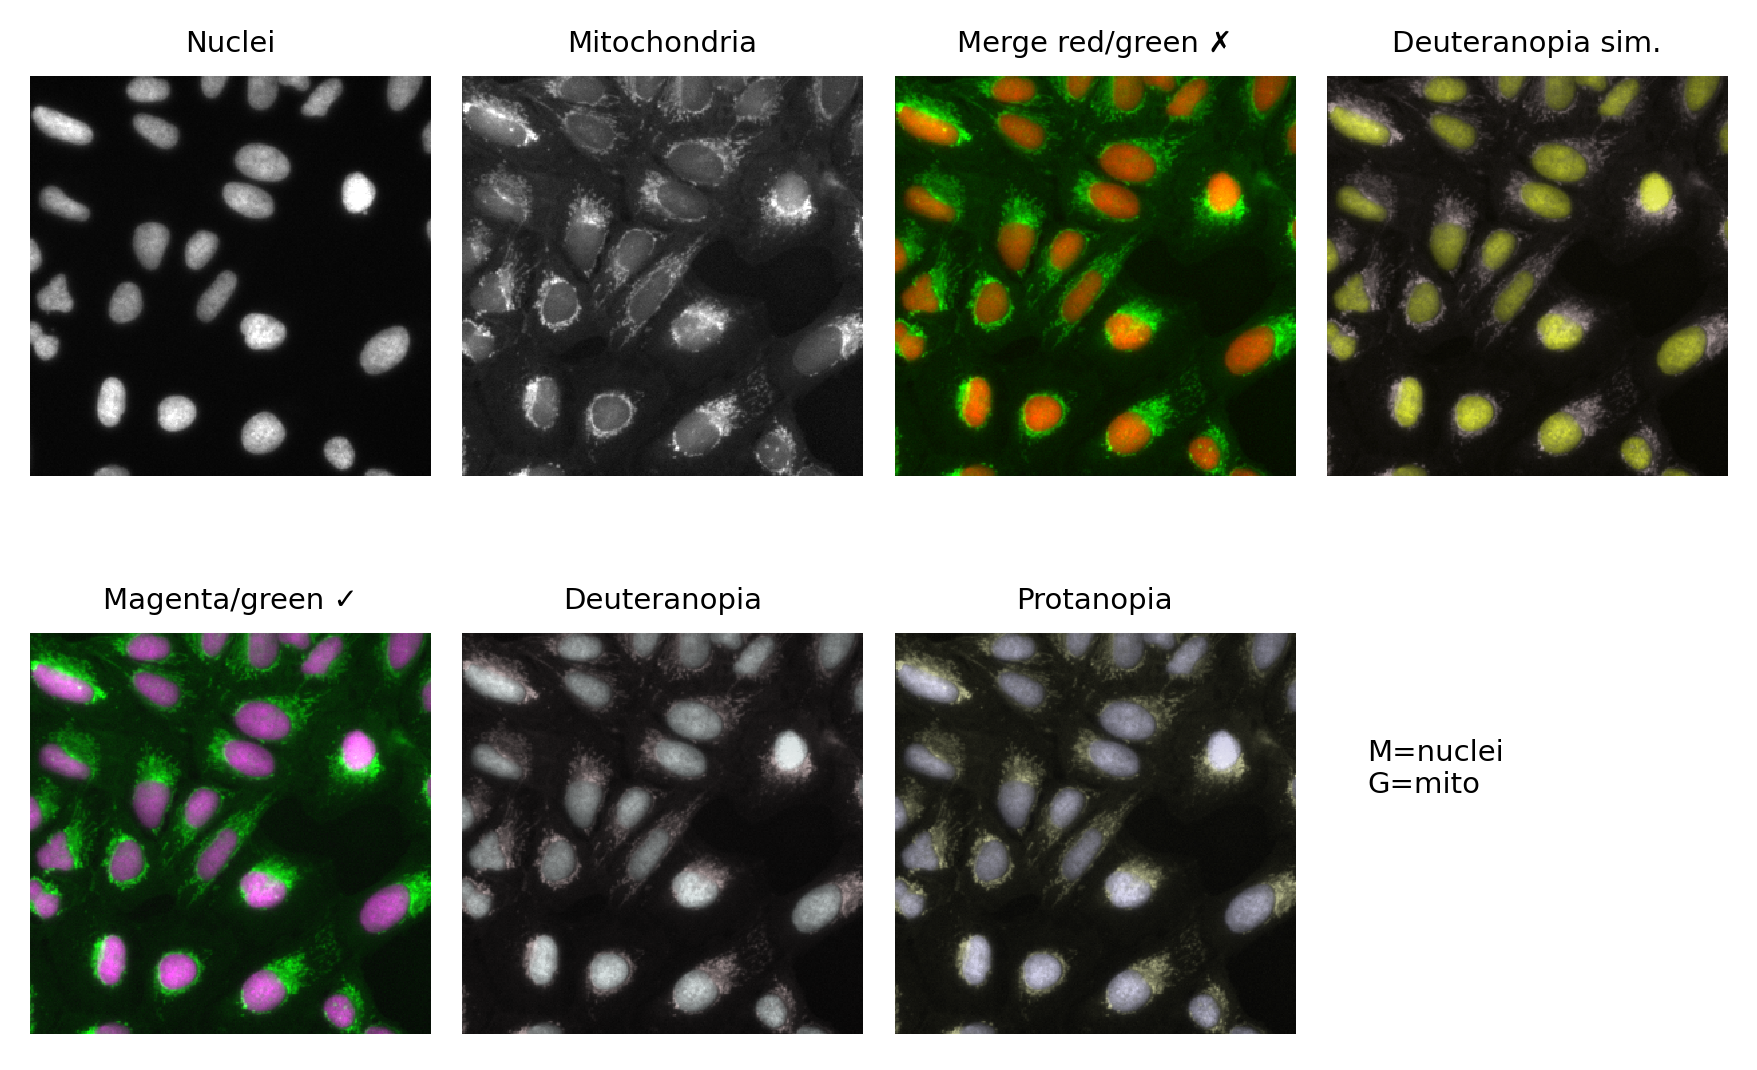
\includegraphics[width=0.88\linewidth]{figures/ch08/ch08-04-pseudocolor-colorblind-en.png}
\caption{Choosing pseudo-colours for multichannel fluorescence. Top: in a red/green merge the two channels become hard to tell apart under simulated deuteranopia. Bottom: a magenta/green merge stays distinguishable under simulated deuteranopia and protanopia. Single-channel greyscale panels need no colour discrimination. Simulation after Machado et al.\ (2009). Image: BBBC022v1, CC0.}\label{fig:ch08-04}
\end{figure}

In the top row of Figure~\ref{fig:ch08-04}, the red/green merge (third column) collapses under simulated deuteranopia (fourth column) into uniform olive-yellow across both nuclei and mitochondria. In the bottom row, the magenta/green merge (first column) preserves clear contrast between slate-violet nuclei and warm olive mitochondria under both simulated deuteranopia (second column) and protanopia (third column). After exporting a figure, authors can also run the \scidraw{} Figure Checker (\sdtool{figure-checker}) to check for colour-vision risks.

\textbf{Second, set and log each channel's linear display range independently before merging.} Nature Portfolio policies require disclosing single-channel adjustments inside a merged image. Mapping each 16-bit channel to 8-bit greyscale via fixed $(v_{\min}, v_{\max})$ bounds in a script before stacking RGB channels---without post-merge colour curves---keeps every parameter exact and reportable.

\textbf{Third, scanning electron micrographs have no native colour; artificial colouration is pseudo-colour and must be declared.} Electron detectors record electron flux as single-channel greyscale. For example, in the public-domain mixed-pollen SEM pair from the Dartmouth Electron Microscope Facility, the archival original (\url{https://commons.wikimedia.org/wiki/File:Misc_pollen.jpg}, $1228 \times 935$ pixels) is greyscale, whereas the colourised version (\url{https://commons.wikimedia.org/wiki/File:Misc_pollen_colorized.jpg}) was hand-tinted afterwards by grain outline. As experimental evidence, SEM images should remain greyscale; if pseudo-colour is applied for illustration, the legend must state that the colours are artificial.

\section{Cropping, Insets, and Scale Bars}

\subsection{Meaning-Preserving Cropping and Zoomed Insets}

Cropping focuses attention on relevant structures, but it must never become ``cherry-picking the brightest or prettiest cell in the field'' (Cromey, 2010; Jambor et al., 2021). Compliant cropping and inset magnification require four practices:
\begin{enumerate}
\item \textbf{Select a representative region and document the criterion:} For a control field, choose a subregion whose nuclear and mitochondrial intensities lie near the field medians, and write that rationale into the processing log.
\item \textbf{Log exact crop coordinates:} Save the pixel bounding box $(x_0, y_0, x_1, y_1)$ in the processing log.
\item \textbf{Mark inset locations on the parent panel and use integer-multiple nearest-neighbour sampling:} Draw a bounding box on the parent image at the exact crop coordinates and state the zoom factor (e.g., $3\times$). Enlarge pixel patches with \textbf{nearest-neighbour interpolation}, expanding each raw pixel into a $k \times k$ block of identical values so the detector's spatial sampling limit remains visible, rather than smoothing edges with bicubic interpolation or ``inventing detail.''
\item \textbf{Never splice separate fields seamlessly:} Images from different fields, time points, or gel lanes must never be abutted to look like one continuous acquisition; legitimate juxtapositions require a clear dividing line and explanation in the legend (Rossner and Yamada, 2004; Bik et al., 2016).
\end{enumerate}

\subsection{Calculating Scale Bars from Calibration Metadata}

The pixel length of a scale bar equals the target physical length divided by the physical pixel size, $L_{\text{px}} = L_{\text{phys}} / s_{\text{px}}$; for an inset enlarged by a factor $k$, the scale-bar pixel length scales by $k$: $L'_{\text{px}} = (L'_{\text{phys}} / s_{\text{px}}) \times k$. Physical pixel size $s_{\text{px}}$ may come only from acquisition metadata, a stage micrometer photographed under identical optics, or an \textbf{instrument data bar} burned into the raw file.

Figure~\ref{fig:ch08-05} demonstrates scale-bar derivation, documented cropping, and nearest-neighbour magnification on a public-domain SEM micrograph of \emph{Nicotiana alata} upper leaf epidermis (\path{Leaf_epidermis.jpg}, $2048 \times 2073$ pixels, 8-bit greyscale), acquired on a Zeiss DSM~962 SEM at $200\times$ by Louisa Howard at the Dartmouth Electron Microscope Facility.

\begin{figure}[htbp]\centering
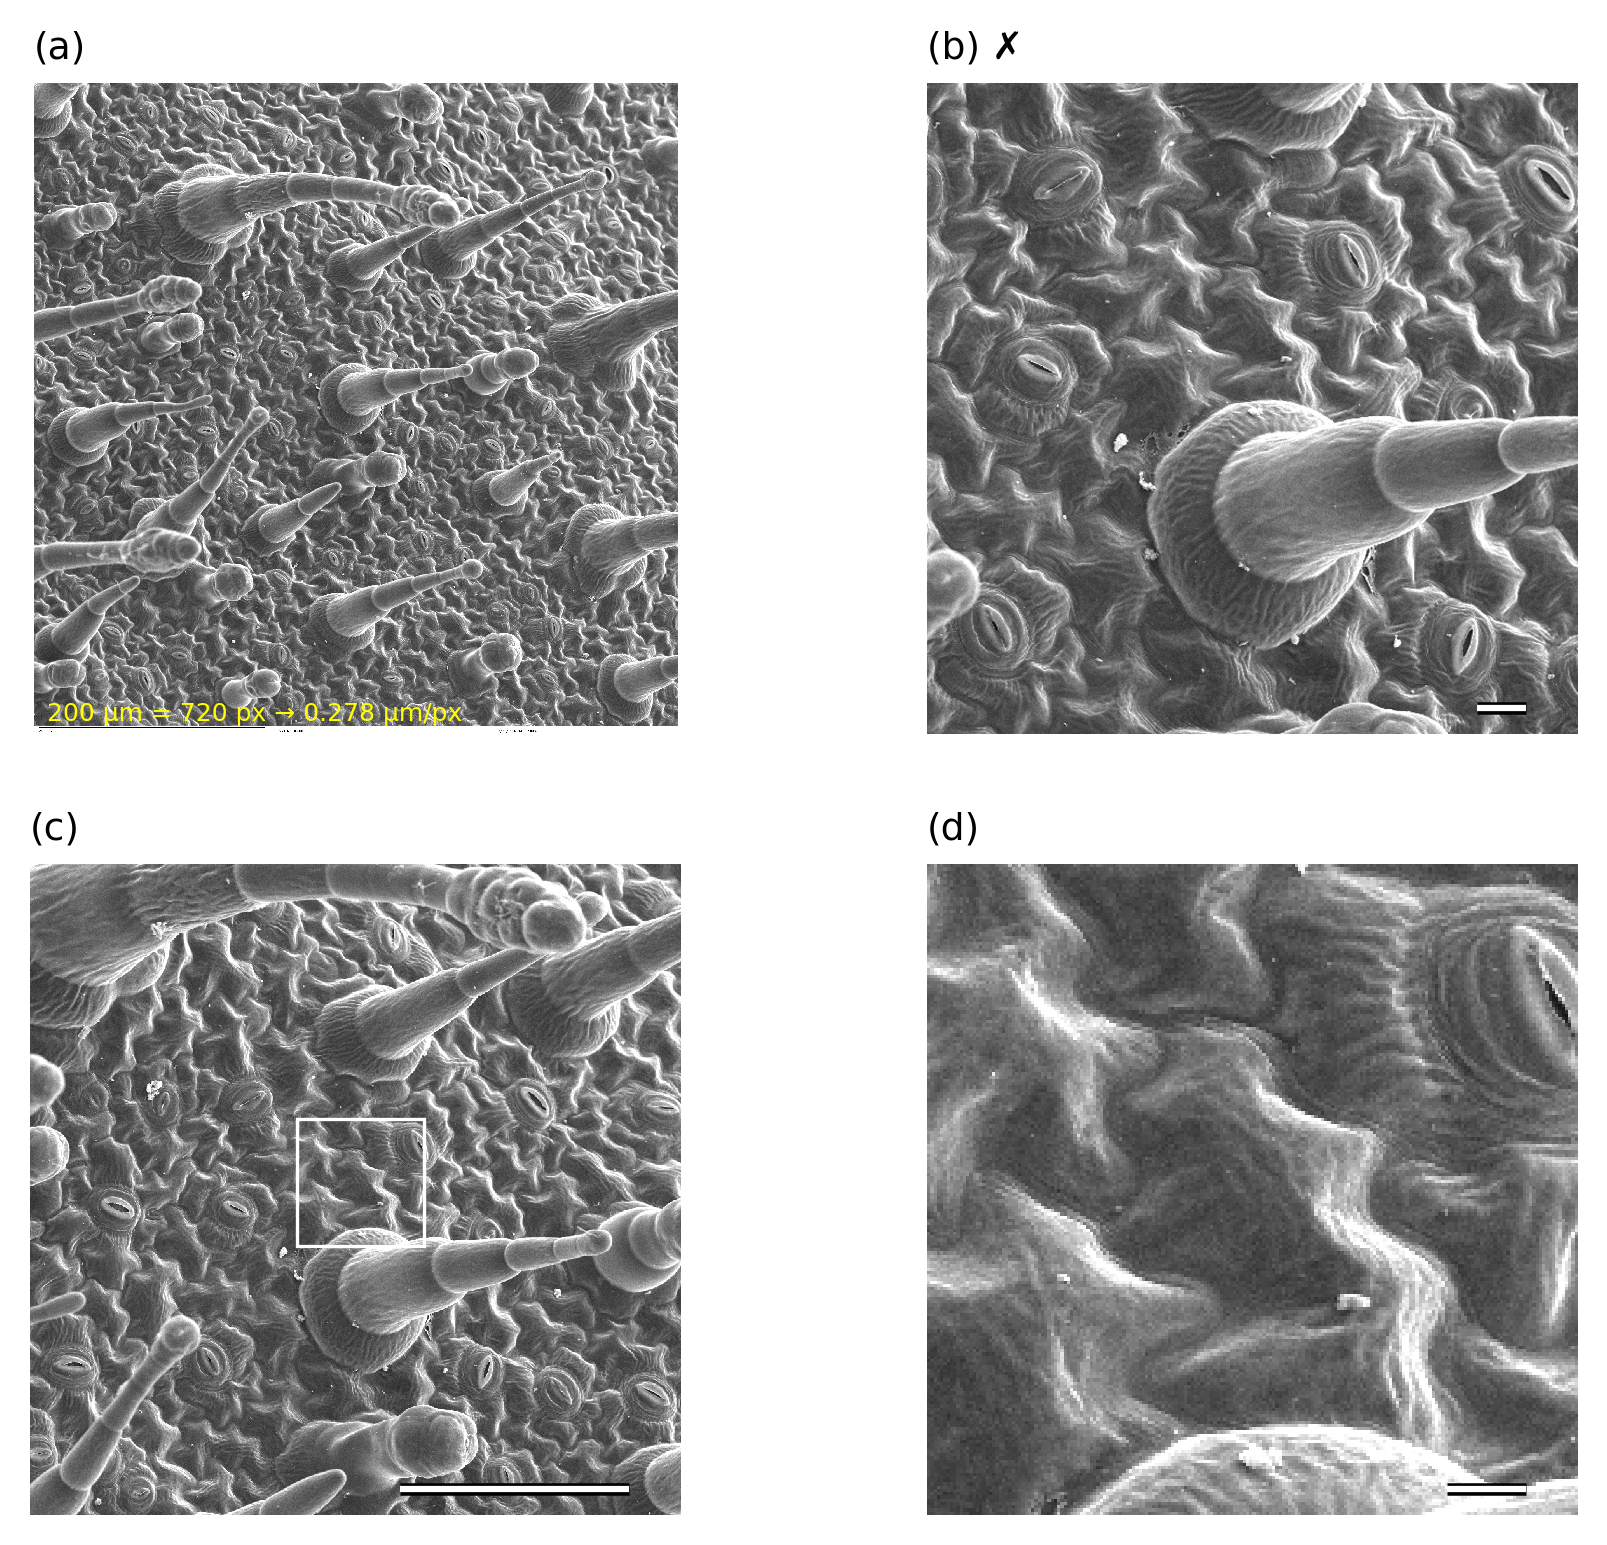
\includegraphics[width=0.88\linewidth]{figures/ch08/ch08-05-crop-inset-scalebar-en.png}
\caption{Cropping, insets and scale bars. (a) Original SEM image (\emph{Nicotiana alata} upper leaf epidermis; Zeiss~962, $200\times$) with the instrument data bar; its $200\ \mu\text{m}$ line spans $720$ pixels, giving $0.278\ \mu\text{m}$ per pixel. (b) Counter-example: data bar removed, a single structure kept, enlarged with bicubic interpolation, and a scale bar drawn without any basis. (c) Recommended: the crop box is recorded and a $100\ \mu\text{m}$ scale bar is drawn from the pixel size; the boxed region is enlarged $3\times$ by nearest-neighbour sampling in (d), scale bar $20\ \mu\text{m}$. Image: Louisa Howard, Dartmouth Electron Microscope Facility, public domain.}\label{fig:ch08-05}
\end{figure}

Comparing the four panels of Figure~\ref{fig:ch08-05} shows how each step is verified:
\begin{itemize}
\item \textbf{Panel (a) (measuring pixel calibration from the instrument data bar):} The bottom $25$ pixel rows (rows $2048\text{--}2072$) form the white data bar generated by the Zeiss DSM~962 SEM, containing a black scale line and the text ``\texttt{200 um},'' ``\texttt{200X},'' ``\texttt{7/31/3 REMF},'' and ``\texttt{Nict.\ leaf \#2.001}.'' Scanning the data bar programmatically for the longest horizontal run of dark pixels (grey value $< 80$) locates the black scale line at rows $2052\text{--}2053$, $x = 15\text{--}734$, spanning exactly \textbf{$720$ pixels}. This gives $s_{\text{px}} = 200\ \mu\text{m} / 720\ \text{px} \approx 0.2778\ \mu\text{m/px}$ (reliant on the microscope's magnification calibration, so the legend states that the scale bar is derived from the instrument data bar). Wikimedia Commons also hosts a third-party derivative (\path{Leaf_epidermis_w_scale.jpg}, $2048 \times 2052$ pixels) with the data bar cropped off and a white ``$200\ \mu\text{m}$'' bar added. Third-party scale bars must always be checked against the primary file: measuring that derivative's white line ($x = 240\text{--}959$) confirms it is $720$ pixels long, matching the original data bar.
\item \textbf{Panel (b) (counter-example):} The data bar is discarded, a single trichome ($600 \times 600$ pixels) is upscaled $4\times$ with bicubic interpolation, and an unverified ``$50\ \mu\text{m}$'' bar is drawn at twice the true calibrated length.
\item \textbf{Panels (c) and (d) (recommended practice):} Panel~(c) logs a $1024 \times 1024$-pixel crop at $(480, 320)\text{--}(1504, 1344)$, draws a calibrated $100\ \mu\text{m} = 360\ \text{px}$ scale bar, and marks a $200 \times 200$-pixel stomatal region at $(900, 720)\text{--}(1100, 920)$ in white; panel~(d) enlarges that box $3\times$ with nearest-neighbour sampling and recalculates the scale bar as $20\ \mu\text{m} = 72 \times 3 = 216\ \text{px}$.
\end{itemize}

\subsection{No Calibration, No Scale Bar}

When an image lacks both calibration metadata and an instrument data bar, the only compliant choice is to \textbf{omit the scale bar and state in the legend that the pixel size is unknown}---never guessing from ``how big a cell usually looks.''

Figure~\ref{fig:ch08-06} shows a three-channel fluorescence micrograph from the NIH ImageJ sample set (\path{FluorescentCells.jpg}, bovine pulmonary artery endothelial cells stained with blue DAPI, green microtubules, and red F-actin; public domain, $512 \times 512$ pixels; also an example of the red/green merge issue from Section~3). Published as an 8-bit lossy JPEG composite with a unitless $1:1$ JFIF density and no objective or pixel size recorded on Commons or the ImageJ source page (panel~a), adding an eyeballed scale bar (panel~b) fabricates scale. Omitting the bar and stating ``pixel size unknown'' in the legend (panel~c) is the honest course. Enlarging the patch $(200, 200)\text{--}(280, 280)$ by $4\times$ with nearest-neighbour sampling (panel~d) exposes $8 \times 8$ JPEG compression blocks and cross-channel bleeding, confirming that the file is a display derivative rather than raw measurement data.

\begin{figure}[htbp]\centering
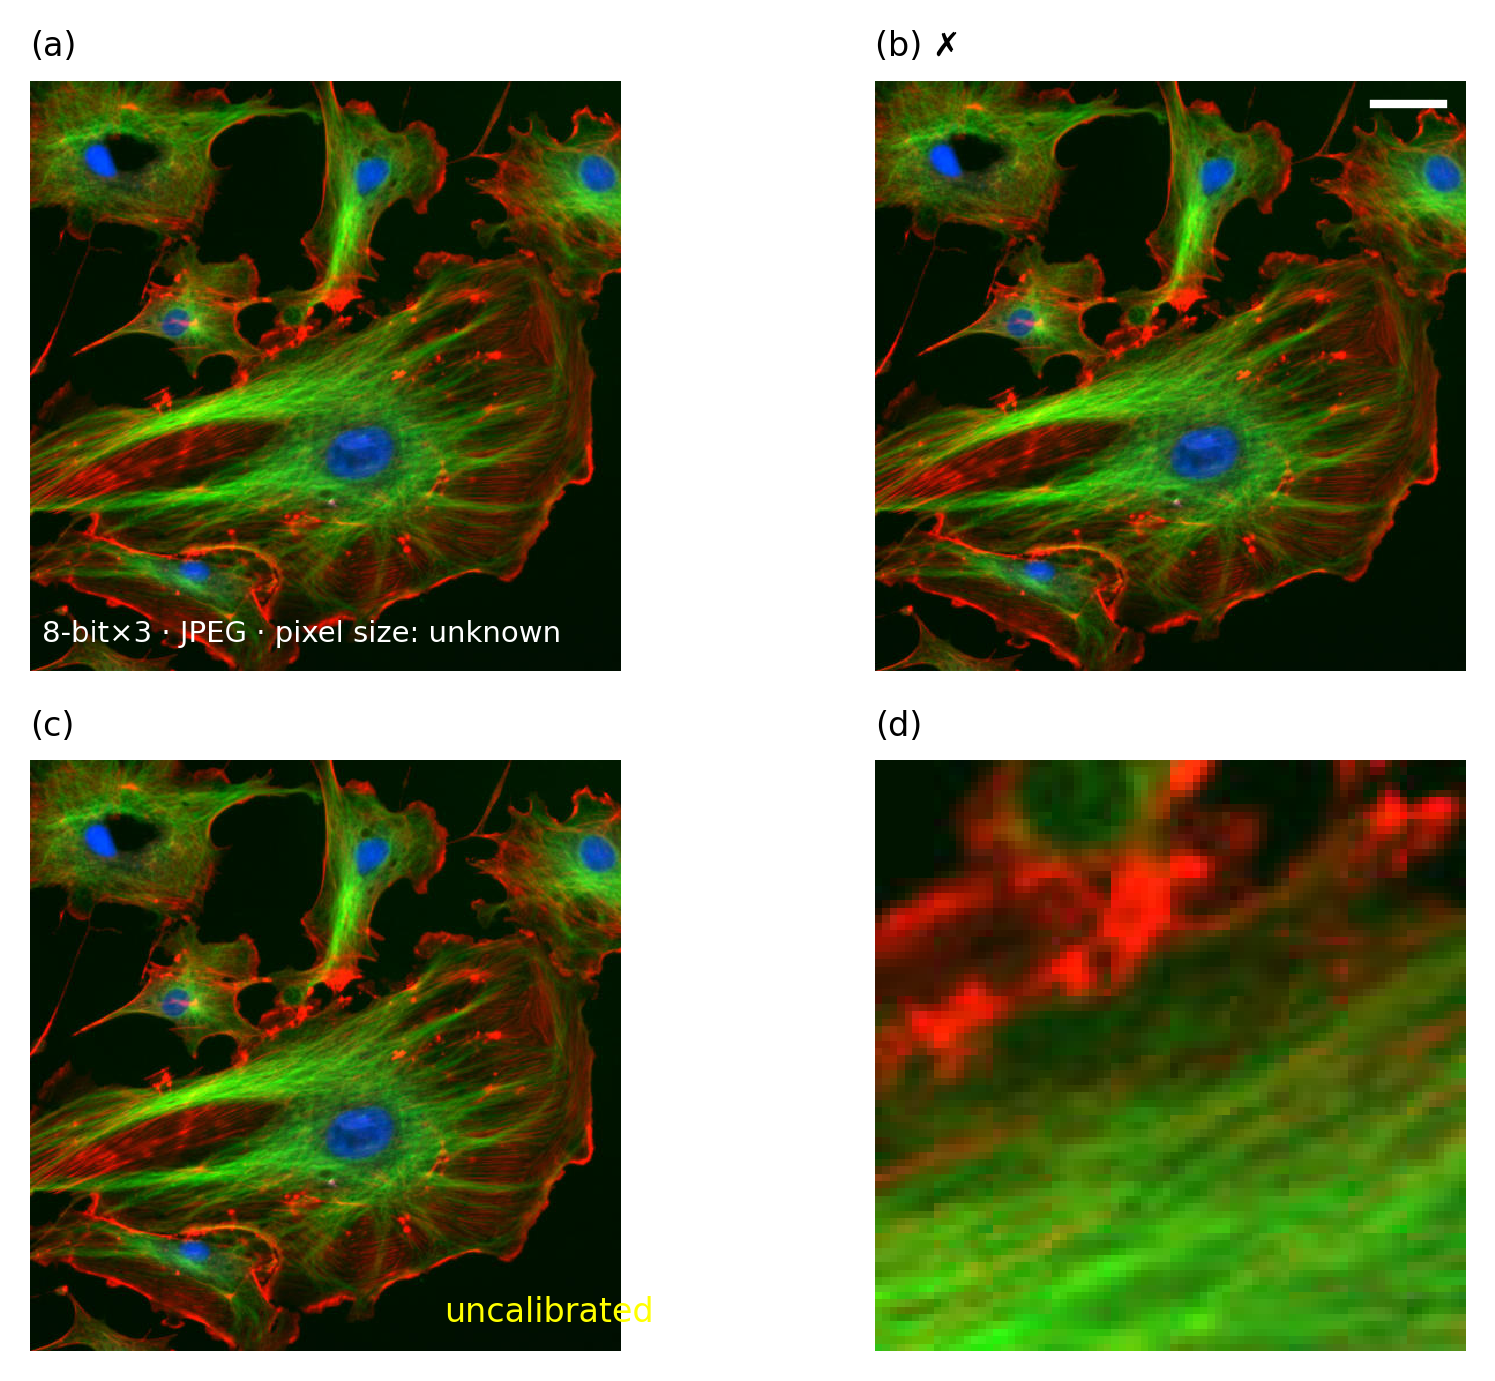
\includegraphics[width=0.88\linewidth]{figures/ch08/ch08-06-no-calibration-en.png}
\caption{No calibration, no scale bar. (a) A three-channel fluorescence image from the ImageJ sample set (bovine pulmonary artery endothelial cells; blue DAPI, green microtubules, red F-actin), published as an 8-bit JPEG composite with no recorded pixel size. (b) Counter-example: a scale bar added by guesswork. (c) Recommended: no scale bar, and the legend states that the pixel size is unknown. (d) Enlargement reveals JPEG compression blocks: the file is a display image, not raw measurement data. Image: public domain (Wikimedia Commons, FluorescentCells.jpg).}\label{fig:ch08-06}
\end{figure}

\section{Journal Rules and the Boundaries of AI}

The \emph{Journal of Cell Biology} guidelines (Rossner and Yamada, 2004) and Cromey's (2010) ethical rules established the baseline for scientific digital images: whole-image adjustments to brightness, contrast, or colour balance are acceptable (with non-linear adjustments disclosed in the caption), but \textbf{no specific feature within an image may be enhanced, obscured, moved, removed, or introduced}. Bik et al.\ (2016) screened $20,621$ biomedical papers and found inappropriate image duplication or manipulation in $3.8\%$, prompting publishers to adopt automated pre-publication image forensics.

In the generative AI era, the Nature Portfolio \emph{Image Integrity and Standards} policy and the Springer Nature \emph{Artificial Intelligence (AI)} policy (both accessed 2026-10-29; because publisher policies evolve rapidly, authors must verify current wording before submission) reinforce these rules: adjustments must be applied across the whole image and equally to controls, must not eliminate data, must disclose pseudo-colouring, non-linear ($\gamma$) mappings, and per-channel adjustments in merges, prohibit clone and healing tools, and classify \textbf{``fabrication of data, citations, or results'' and ``generation of photorealistic images (deepfakes)'' as impermissible}.

Why does passing a blurry micrograph to a generative model to ``denoise and sharpen'' count as fabricating data? We tested this with a ground-truth experiment on the \emph{Nicotiana alata} SEM micrograph from Figure~\ref{fig:ch08-05} (Figure~\ref{fig:ch08-07}):
\begin{enumerate}
\item Crop a $512 \times 512$-pixel patch $(640, 680)\text{--}(1152, 1192)$ from the original SEM image as \textbf{ground truth (GT, panel~a)}, containing three stomata, epidermal cell ridges, the base of a large right trichome, and a small lower-left trichome.
\item Downsample $4\times$ by $4 \times 4$ area averaging to produce a $128 \times 128$-pixel low-resolution input \textbf{LR (panel~b, nearest-neighbour display)}.
\item \textbf{Control~1 (panel~c):} Upscale LR back to $512 \times 512$ pixels with deterministic bicubic interpolation (blurry, but adds no new structures).
\item \textbf{Control~2 (panel~d):} Pass the same $128 \times 128$ LR image to an image-generation model in image-editing mode three independent times with a typical naive user prompt (to avoid cherry-picking the worst run, panel~d shows Run~1 and Runs~2 and~3 are archived):
\end{enumerate}

\begin{Prompt}
Upscale this grayscale scanning electron microscope image to 512 x 512 pixels.
Make it sharper and more detailed, remove blur and noise, and enhance the fine
surface structures so it looks like a high-resolution micrograph.
Keep it grayscale. Do not add any text, letters, numbers, labels, or scale bars.
Square 1:1 aspect ratio.
\end{Prompt}

\begin{figure}[htbp]\centering
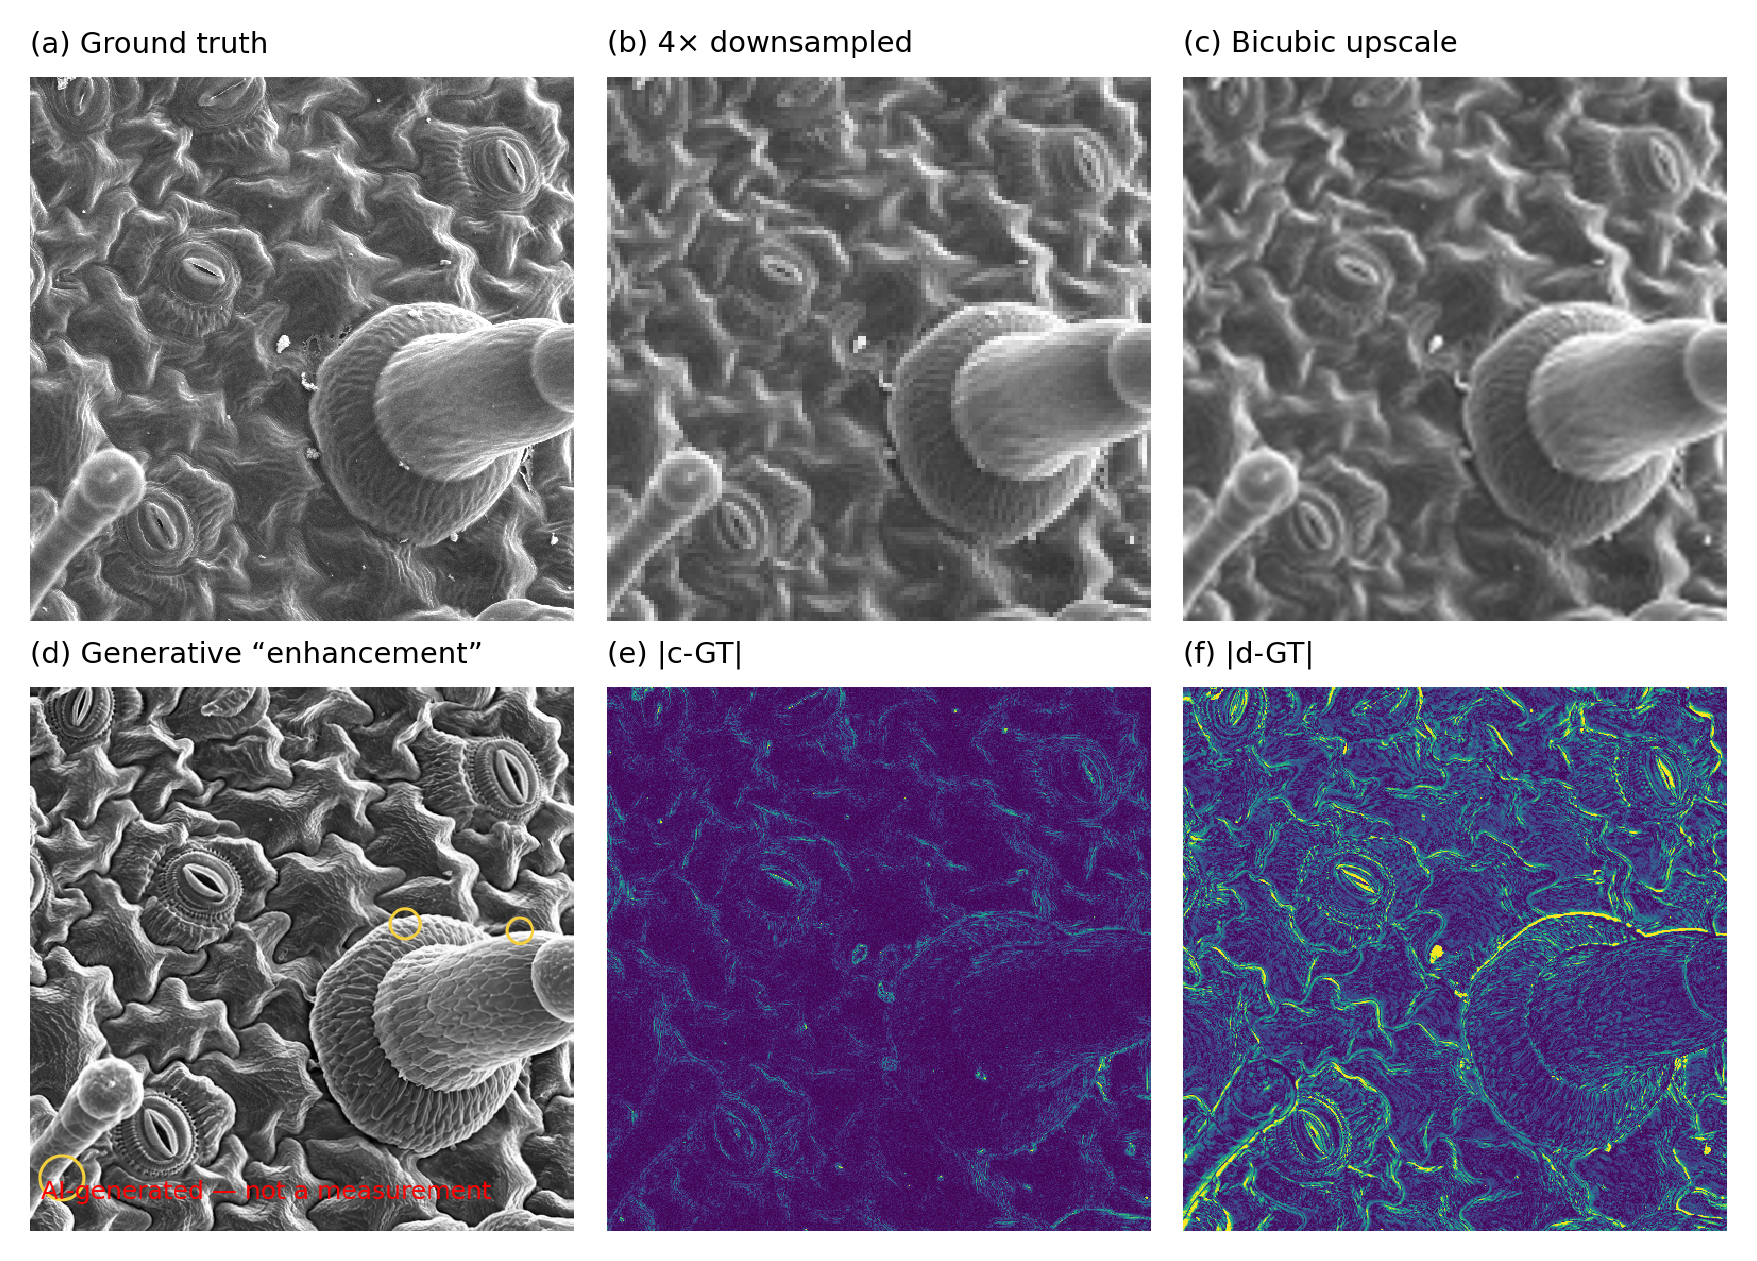
\includegraphics[width=0.88\linewidth]{figures/ch08/ch08-07-generative-risk-en.png}
\caption{Generative ``enhancement'' invents structure. (a) Crop of the original SEM image (ground truth). (b) The same crop downsampled $4\times$. (c) Bicubic upscaling: blurry, but nothing new is added. (d) Upscaling by an image-generation model asked to ``make it sharper and more detailed'': it looks crisper yet contains edges and textures absent from the original (circles). (e, f) Absolute differences of (c) and (d) from the original. The generated image illustrates the risk only and must never be used as experimental data. Original: Louisa Howard, Dartmouth Electron Microscope Facility, public domain; panel (d) was generated by an image model (prompt and generation log in the book repository).}\label{fig:ch08-07}
\end{figure}

Comparing the six panels of Figure~\ref{fig:ch08-07} and the three runs reveals four distortions common to any generative upscaler:
\begin{itemize}
\item \textbf{Loss of control over dimensions and channel mode:} Although the prompt requested a $512 \times 512$ single-channel greyscale image, all three runs returned $1254 \times 1254$-pixel ($9.8\times$) three-channel 8-bit RGB files with inter-channel spreads up to $10\text{--}12$ grey levels.
\item \textbf{Fabricated anatomical boundaries and textures:} Panel~(d) looks sharper than bicubic upscaling (c), but comparison against ground truth (a) reveals invented multi-ringed collars and serrated teeth around the upper-left stomatal pore, plus dense scale-like striations across the right trichome and cuticle. At the three yellow circles on panel~(d)---two crease ridges on the upper basal collar of the large trichome (near $(353, 222)$ and $(460, 229)$) and the tip of the lower-left trichome (near $(30, 461)$)---the model hallucinated bright rims and boundaries absent from the specimen.
\item \textbf{Contradictory details across repeated runs:} From the exact same $128 \times 128$ input, Run~1 synthesized tight scale-like strips, Run~2 produced rounded pebble-like granules and split the lower-left trichome tip into polygonal blocks, and Run~3 drew radiating pleats around the large trichome base---proving these high-frequency details are stochastic texture synthesis rather than specimen measurements.
\item \textbf{Pixel-wise error nearly triple that of bicubic interpolation:} Converting Run~1 to greyscale, resizing to $512 \times 512$ with Lanczos solely for comparison, and applying rigid registration ($-0.5^\circ$ rotation, $dx = -1, dy = +1$ pixel) yields the difference maps in panels~(e) and~(f) (shared $0\text{--}128$ \texttt{viridis} scale). Bicubic interpolation $|c - \text{GT}|$ (panel~e) has a mean absolute error (MAE) of $10.32$ grey levels, whereas generative upscaling $|d - \text{GT}|$ (panel~f) reaches an MAE of $28.91$ after registration ($29.06$ before registration).
\end{itemize}

The conclusion is absolute: \textbf{AI can help you write processing scripts, draft methods, and check colour vision, but it must never generate a single pixel that will be treated as a measurement.}

\section{Complete Case Study: Presenting Control-Field Images of U2OS Cells}

We now walk through Su's supplementary methods figure from raw TIFFs to verified delivery. Supplementary Figure~S1 shows the nuclear and mitochondrial staining patterns of U2OS cells under DMSO control (\texttt{mock}) conditions so peers can judge raw image quality for downstream profiling. It \textbf{reports no treatment effect}, and because it uses the benchmark dataset BBBC022v1 (Gustafsdottir et al., 2013), acquisition parameters cite the dataset documentation ($20\times$ objective, $0.656\ \mu\text{m/pixel}$) and primary paper without inventing unrecorded settings.

\textbf{Step~1: Build the raw-image catalogue (Deliverable~1).} Lock the four 16-bit TIFFs for well A13 sites \texttt{s1} and \texttt{s2} as read-only, verify SHA-256 hashes by script, and generate the raw-image catalogue (Table~\ref{tab:ch08-catalog} and companion CSV).

\begin{table}[htbp]\centering\footnotesize
\setlength{\tabcolsep}{3pt}
\renewcommand{\arraystretch}{1.15}
\caption{Raw-image catalogue for the case study (site~1 channels shown; site~2 \texttt{w1} spans $122\text{--}1450$, mean $227.1$, $p_{0.1}/p_{99.9}=129/1150$, and \texttt{w5} spans $176\text{--}1655$, mean $366.3$, $p_{0.1}/p_{99.9}=196/1078$, logged in the companion CSV).}\label{tab:ch08-catalog}
\begin{tabularx}{\linewidth}{@{}>{\raggedright\arraybackslash}p{25mm}YY@{}}
\toprule
\textbf{Field} & \textbf{Example: s1 Hoechst (w1)} & \textbf{Example: s1 MitoTracker (w5)} \\
\midrule
Filename & \path{IXMtest_A13_s1_w1B35C6D5D-DBF9-4779-990D-5E7AFB14D600.tif} & \path{IXMtest_A13_s1_w5B257EE32-37B0-4698-891B-11B1B3D3D0C1.tif} \\
Source & BBBC022v1, plate 20585, well A13 (\texttt{mock}), site~1 & BBBC022v1, plate 20585, well A13 (\texttt{mock}), site~1 \\
Channel / dye & w1 / Hoechst 33342 (DNA) & w5 / MitoTracker Deep Red (mitochondria) \\
Dimensions / depth & $696 \times 520\ \text{px}$, 16-bit container, 12-bit effective & $696 \times 520\ \text{px}$, 16-bit container, 12-bit effective \\
Pixel size & $0.656\ \mu\text{m}$ (dataset docs, $20\times$) & $0.656\ \mu\text{m}$ (dataset docs, $20\times$) \\
SHA-256 (first 16) & \texttt{4be40f814481002a} (full 64-hex in CSV) & \texttt{c1c441e44e91481c} (full 64-hex in CSV) \\
Raw value range & $121\text{--}1655$; $p_{0.1}/p_{99.9}=132/1236$; saturated: $0$ & $185\text{--}4095$; $p_{0.1}/p_{99.9}=218/1140$; saturated: $12$ \\
License \& status & CC0 1.0; read-only master, processed on copies & CC0 1.0; read-only master, processed on copies \\
\bottomrule
\end{tabularx}
\end{table}

\textbf{Step~2: Write the figure brief (Deliverable~2).} Write the brief below in your own document and save it; you will refer to it after choosing ``Multi-panel figure'' in the \scidraw{} Scientific Figure Workflow wizard (\sdtool{figure-workflow}) and following the route into the Multi-Panel Figure Maker (\sdtool{multi-panel-figure-maker}):

\begin{Prompt}
[Purpose & Audience] Supplementary methods figure (Supplementary Fig. S1), double-column
width 174 mm; for cell-imaging peers evaluating raw image and staining quality.
[Goal] Show nuclear (Hoechst 33342) and mitochondrial (MitoTracker Deep Red) staining
patterns of U2OS cells under DMSO control conditions; no treatment effect is reported.
[Source Material] BBBC022v1 (CC0), plate 20585, well A13 (mock), site s1; channels w1, w5;
16-bit TIFF, 696 x 520 px, 0.656 um/pixel (dataset docs). Originals read-only; SHA-256 logged.
[Panels] a, Nuclei (greyscale); b, Mitochondria (greyscale); c, Merge (nuclei magenta,
mitochondria green); d, Enlarged inset of a subregion in c (marked by a white box on c).
[Allowed Processing] Whole-image linear display mapping (black/white points), pseudo-colour
LUT, cropping, integer-multiple nearest-neighbour enlargement. One display range per channel
shared across all panels and written to the processing log.
[Prohibited] Gamma or curves, denoising, sharpening, deconvolution, background subtraction,
local adjustments, or any generative "enhancement".
[Scale Bars & Selection] From 0.656 um/pixel: 50 um on a-c, recalculated 10 um on d; white
solid bars at bottom right, length stated in legend. Select a typical cell near field median
intensities for d; report the 12 saturated pixels (4095) in w5 without retouching.
[Export & Verification] Lossless 8-bit PNG panels assembled in SciDraw AI Multi-Panel Figure
Maker (TIFF/PDF + log); trace SHA-256, verify scale bars and deuteranopia separability.
\end{Prompt}

\textbf{Step~3: Use a general-purpose AI assistant to organize the presentation plan and draft the processing script.} Submit the following prompt to a general-purpose AI chat assistant to generate the plan and deterministic Python script:

\begin{Prompt}
I have two raw 16-bit fluorescence micrographs and need a supplementary methods figure.
Before writing code, outline a presentation plan: what each panel shows, whether each step
is a linear operation, and what must be disclosed in the processing log and figure legend.
Images: two 16-bit greyscale TIFFs, 696 x 520 px; w1 = Hoechst 33342 (nuclei),
w5 = MitoTracker Deep Red (mitochondria); pixel size 0.656 um (dataset documentation);
effective 12-bit camera data, with 12 saturated pixels (4095) in w5.
Requirements:
1. Use whole-image linear display mapping only; set black/white points by raw percentiles.
2. Merge with magenta (nuclei) and green (mitochondria), explaining why red/green is avoided.
3. Compute scale-bar lengths in pixels from 0.656 um/px, recalculating for the zoomed inset.
4. List prohibited operations (denoising, sharpening, gamma, local edits, generative upscale).
5. List every item I must verify manually.
Once the plan is confirmed, write a Python script that reads the originals read-only and saves
display ranges, crop coordinates, zoom factor, scale-bar pixels, and SHA-256 to processing-log.json.
\end{Prompt}

Never copy percentile thresholds or pixel lengths estimated in chat prose; let the script compute them directly on the real 16-bit TIFF arrays and write them to \path{processing-log.json}. Run the script on a copy first and inspect the code to confirm no denoising, sharpening, or gamma functions are called.

\textbf{Step~4: Audit the five flaws in the first draft (\texttt{v1}) and issue a revision order.} Figure~\ref{fig:ch08-08} shows an ad hoc first draft counter-example with five numbered flaws:
\begin{enumerate}
\item \textbf{Issue~1 (auto-contrast per panel):} Panels~\textbf{a} and~\textbf{b} are stretched separately to their own \texttt{min--max}, and the merge in~\textbf{c} uses another mapping, leaving no unified parameters to report.
\item \textbf{Issue~2 (red--green merge):} Panel~\textbf{c} merges red and green, which become hard to distinguish under simulated red--green colour-vision deficiency.
\item \textbf{Issue~3 (unfounded scale bar):} The ``$20\ \mu\text{m}$'' bar at the bottom right of~\textbf{c} is $50\ \text{px}$ long, whereas at $0.656\ \mu\text{m/px}$ a true $20\ \mu\text{m}$ bar is $30.5\ \text{px}$---$64\%$ too long.
\item \textbf{Issue~4 (brightest cell + bicubic interpolation):} Inset~\textbf{d} cherry-picks the brightest, most atypical condensed nucleus in the field (coordinates $x = 488\text{--}552$, $y = 184\text{--}248$), upscales it $4\times$ with bicubic interpolation, and omits a locator box on~\textbf{c}.
\item \textbf{Issue~5 (undisclosed $\gamma = 0.6$ and lossy export):} The mitochondrial channel applies an undisclosed $\gamma = 0.6$ boost and exports as a quality-70 JPEG.
\end{enumerate}

\begin{figure}[htbp]\centering
\resizebox{0.88\linewidth}{!}{% FIG ch08-08 v1 issue overlay (English).
% Numbered marks sit on the panel each problem belongs to.
% The phrases are listed under the micrograph so they do not cover it.
\tikzset{%
  chviiiissue/.style={%
    circle, draw=BookInk, line width=0.4pt, fill=white, inner sep=0.2pt,%
    minimum size=9pt, font=\sffamily\fontsize{7}{8}\selectfont, text=BookInk%
  },%
  chviiicap/.style={%
    anchor=west, inner xsep=0.4pt, inner ysep=0.5pt,%
    font=\sffamily\fontsize{7}{9}\selectfont, text=BookInk%
  }%
}
\providecommand{\chviiimark}[1]{%
  \tikz[baseline=(n.base)]{\node[chviiiissue] (n) {#1};}%
}
\begin{tikzpicture}
  \node[anchor=south west, inner sep=0pt] (img) at (0,0)
    {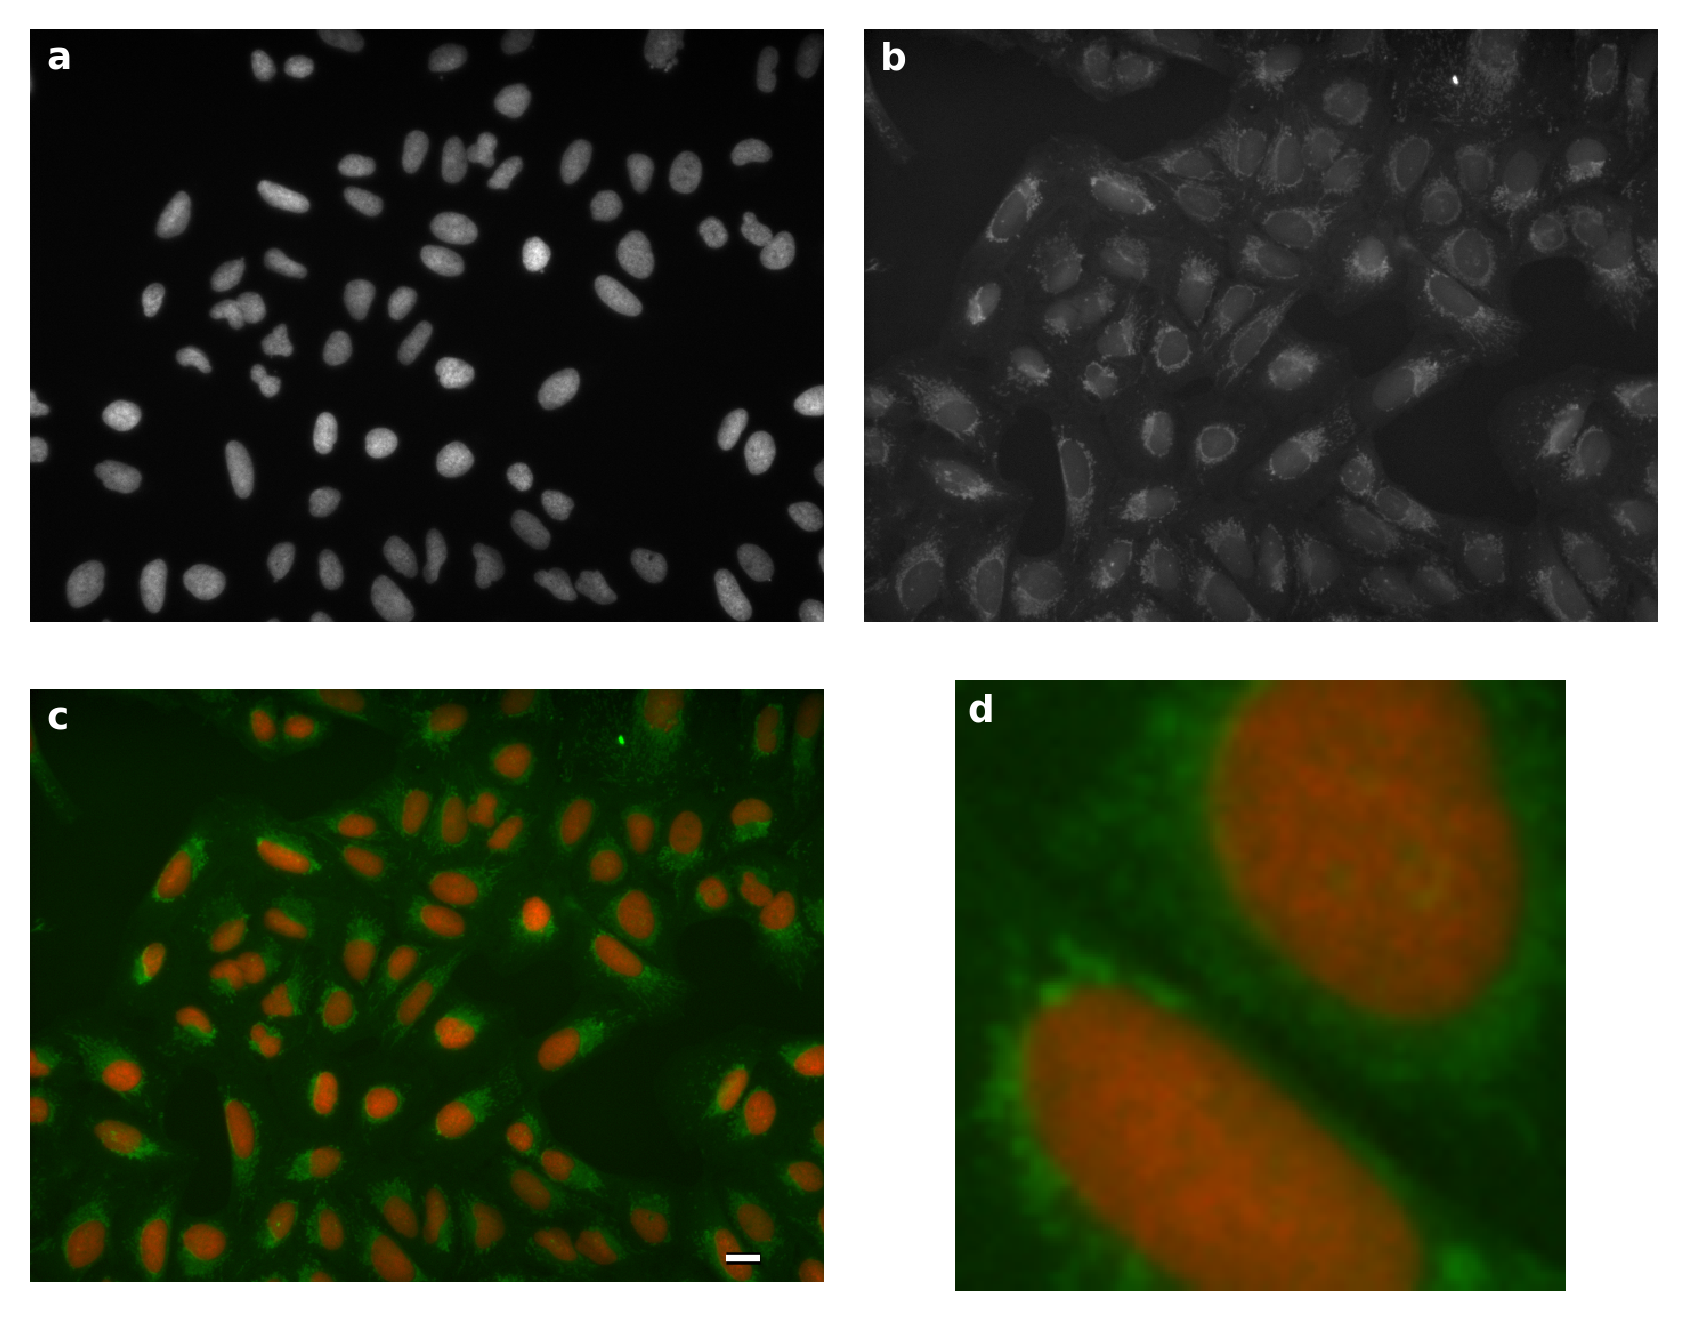
\includegraphics[width=\linewidth]{figures/ch08/ch08-08-case-v1-en.png}};
  \begin{scope}[x={(img.south east)}, y={(img.north west)}]
    \node[chviiiissue] (m1) at (0.40, 0.92) {1};
    \node[chviiiissue] (m2) at (0.40, 0.45) {2};
    \node[chviiiissue] (m3) at (0.36, 0.09) {3};
    \draw[BookInk, line width=0.35pt] (0.372, 0.078) -- (0.424, 0.056);
    \node[chviiiissue] (m4) at (0.88, 0.12) {4};
    \node[chviiiissue] (m5) at (0.90, 0.92) {5};
  \end{scope}
  \node[chviiicap] (c1) at ([yshift=-1.8mm]img.south west)
    {\chviiimark{1}\enspace auto-contrast per panel};
  \node[chviiicap] (c2) at ([yshift=-0.8mm]c1.south west)
    {\chviiimark{2}\enspace red--green};
  \node[chviiicap] (c3) at ([yshift=-0.8mm]c2.south west)
    {\chviiimark{3}\enspace unfounded scale bar};
  \node[chviiicap] (c4) at ([yshift=-0.8mm]c3.south west)
    {\chviiimark{4}\enspace brightest cell + bicubic};
  \node[chviiicap] (c5) at ([yshift=-0.8mm]c4.south west)
    {\chviiimark{5}\enspace undisclosed $\gamma=0.6$};
\end{tikzpicture}
}
\caption{Five common problems in a first draft (numbered 1--5; see text). This version was produced deliberately with wrong settings as a teaching counter-example. The legend for the final version is given in the case section.}\label{fig:ch08-08}\label{fig:ch08-08-v1}
\end{figure}

Against these five flaws, we issue an itemized revision order:

\begin{Prompt}
Revision Order (v1 -> final)
1. Fix one linear display range per channel across all panels:
   Hoechst black point 132, white point 1236 (raw p0.1 / p99.9);
   MitoTracker black point 218, white point 1140 (raw p0.1 / p99.9). Share in the merge.
2. Remove gamma; use strictly linear mapping and log "linear_no_gamma: true".
3. Change merge LUT to magenta nuclei (R+B) and green mitochondria (G); verify under
   deuteranopia and protanopia simulation.
4. Recalculate scale bars from 0.656 um/pixel: 50 um = 76.2 px (panels a-c);
   for panel d (3x nearest-neighbour enlargement), 10 um = 15.24 px x 3 = 45.7 px.
5. Move the inset crop in d to a representative cell near median nuclear and mitochondrial
   intensities at pixel coordinates (280, 328)-(344, 392); draw a white locator box on c.
6. Enlarge d by 3x using nearest-neighbour sampling only (no bicubic or "detail enhancement").
7. Export lossless 8-bit PNG panels; archive raw 16-bit TIFFs, script, and processing-log.json.
8. Disclose in both processing log and legend that 12 pixels in w5 saturated at acquisition (4095).
\end{Prompt}

\textbf{Step~5: Assemble in the \scidraw{} Multi-Panel Figure Maker, merge the two-tier processing logs, and complete verification.} Once the script generates four lossless 8-bit PNG panels and \path{processing-log.json}, open the \scidraw{} Multi-Panel Figure Maker (\sdtool{multi-panel-figure-maker}): import the four panels, choose a double-column preset ($174\ \text{mm}$ width, such as Cell or Springer), set a $2 \times 2$ grid with automatic labels \textbf{a}--\textbf{d} (any in-tool cropping or rotation is also logged), and export the ZIP package (TIFF, PNG, PDF, PPTX, and assembly log) to produce the final figure (Figure~\ref{fig:ch08-09}).

\begin{figure}[htbp]\centering
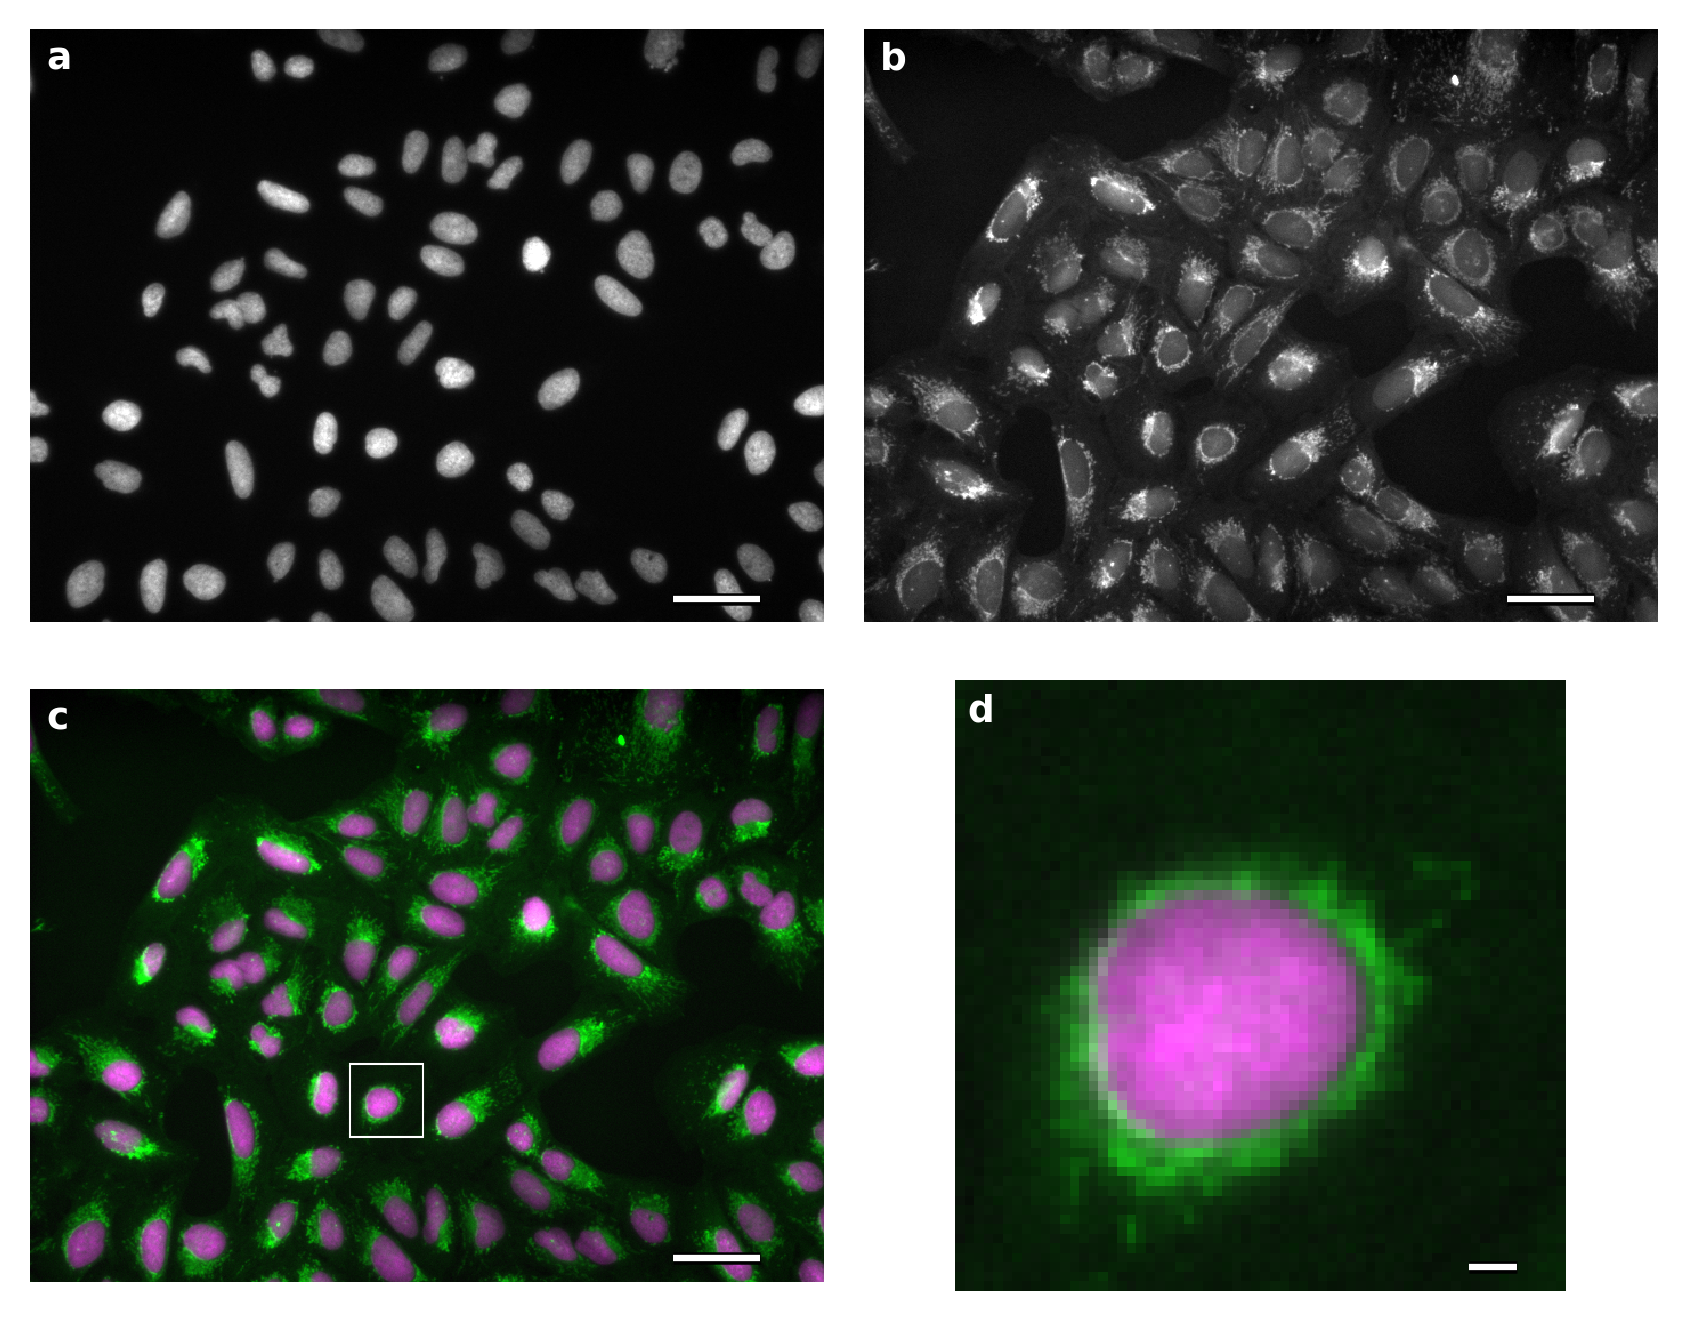
\includegraphics[width=0.88\linewidth]{figures/ch08/ch08-08-case-final-en.png}
\caption{Supplementary Fig.\ S1 | Nuclear and mitochondrial staining of U2OS cells under DMSO control conditions. \textbf{a}, Hoechst~33342 (nuclei). \textbf{b}, MitoTracker Deep Red (mitochondria). \textbf{c}, Merge (nuclei magenta, mitochondria green); the white box marks the region shown in~\textbf{d}. \textbf{d}, The boxed region in~\textbf{c} enlarged $3\times$ with nearest-neighbour sampling. Images are from BBBC022v1 (plate 20585, well A13, site~1; CC0; Gustafsdottir et al., 2013), acquired with a $20\times$ objective at $0.656\ \mu\text{m}$ per pixel. All panels use whole-image linear display mapping with no gamma or other non-linear adjustment; display ranges were $132\text{--}1236$ (Hoechst) and $218\text{--}1140$ (MitoTracker) in raw 12-bit values and are identical for each channel across panels. Twelve pixels in the mitochondrial channel were saturated at acquisition ($4095$) and were not altered. Scale bars, $50\ \mu\text{m}$ (\textbf{a}--\textbf{c}) and $10\ \mu\text{m}$ (\textbf{d}). Raw 16-bit images, the processing script and the processing log are provided as Supplementary Data.}\label{fig:ch08-09}\label{fig:ch08-08-final}
\end{figure}

At this step, the author must verify two critical platform boundaries:
\begin{enumerate}
\item \textbf{Merge the upstream processing log with the multi-panel assembly log:} The assembly log exported by \sdtool{multi-panel-figure-maker} records each panel's filename, SHA-256 hash, original dimensions and bit depth, crop box, rotation or flip, physical millimetre width, effective resolution, and resampling mode, and states: ``Apart from the cropping, rotation, and scaling recorded above, no brightness, contrast, colour, or content modifications were applied to any panel.'' Crucially, \textbf{this statement covers only operations inside the multi-panel tool.} Because the imported PNG panels already underwent upstream intensity mapping and pseudo-colour merging in the script---and because the multi-panel tool currently does not generate calibrated scale bars, channel labels, or linked inset boxes, nor does its ZIP bundle the raw 16-bit TIFFs---the author must \textbf{merge} the script's \path{processing-log.json} with the assembly log into one complete processing record so readers are not misled into thinking no display adjustment occurred.
\item \textbf{Check effective resolution honestly and complete the figure legend:} A $696\ \text{px}$-wide raw image spans about $59\ \text{mm}$ at $300\ \text{dpi}$; in a $174\ \text{mm}$-wide $2 \times 2$ grid where each panel is roughly $85\ \text{mm}$ wide, the effective resolution is about $208\ \text{dpi}$. Authors must either accept this lower effective resolution and state the native pixel dimensions transparently, or reduce the panel width to reach $300\ \text{dpi}$---\textbf{never upscaling by interpolation to fake higher resolution}. Next, run the Figure Checker (\sdtool{figure-checker}) to check file format, resolution, greyscale contrast, and colour-vision risks (noting that it performs technical checks rather than scientific review), and use the Figure Legend assistant (\sdtool{figure-legend}) to draft a description of visible features before manually adding fluorophores, pixel size, display windows, saturation counts, and scale-bar lengths (by design, the tool never invents magnification, scale bars, or methods).
\end{enumerate}

\begin{Prompt}
Supplementary Fig. S1 | Nuclear and mitochondrial staining of U2OS cells under DMSO control
conditions. a, Hoechst 33342 (nuclei). b, MitoTracker Deep Red (mitochondria). c, Merge
(nuclei magenta, mitochondria green); the white box marks the region shown in d. d, The
boxed region in c enlarged 3x with nearest-neighbour sampling. Images are from BBBC022v1
(plate 20585, well A13, site 1; CC0; Gustafsdottir et al., 2013), acquired with a 20x
objective at 0.656 um per pixel. All panels use whole-image linear display mapping with no
gamma or other non-linear adjustment; display ranges were 132-1236 (Hoechst) and 218-1140
(MitoTracker) in raw 12-bit values and are identical for each channel across panels. Twelve
pixels in the mitochondrial channel were saturated at acquisition (4095) and were not
altered. Scale bars, 50 um (a-c) and 10 um (d). Raw 16-bit images, the processing script
and the processing log are provided as Supplementary Data.
\end{Prompt}

\begin{table}[htbp]\centering\footnotesize
\setlength{\tabcolsep}{3pt}
\renewcommand{\arraystretch}{1.15}
\caption{Verification audit for the final case-study figure (Supplementary Fig.\ S1).}\label{tab:ch08-verify}
\begin{tabularx}{\linewidth}{@{}>{\raggedright\arraybackslash}p{25mm}YY@{}}
\toprule
\textbf{Verification item} & \textbf{Audit method} & \textbf{Measured result} \\
\midrule
Input file hashes & Script asserts SHA-256 of four panels against catalogue & Matches Table~\ref{tab:ch08-catalog} and catalogue CSV; originals unmodified \\
Display range \& linearity & Cross-check \path{processing-log.json} against figure legend & Hoechst $132\text{--}1236$, MitoTracker $218\text{--}1140$, linear with no $\gamma$, 12 saturated pixels reported \\
Scale-bar pixel lengths & Recompute from $0.656\ \mu\text{m/px}$ and measure on exported figure & Panels \textbf{a}--\textbf{c}: $50\ \mu\text{m} = 76.2\ \text{px}$; panel \textbf{d} ($3\times$): $10\ \mu\text{m} = 45.7\ \text{px}$; exact match \\
Inset \& crop coordinates & Compare white box on \textbf{c} with crop coordinates of \textbf{d} & Shared median-cell coordinates $(280, 328)\text{--}(344, 392)$, $3\times$ nearest-neighbour sampling \\
Colour vision \& log merge & Machado (2009) simulation, \sdtool{figure-checker}, and dual-log check & Magenta/green separable under red--green deficiency; upstream and assembly logs merged \\
\bottomrule
\end{tabularx}
\end{table}

\section{What AI Can and Cannot Do in Presenting Experimental Images}

Table~\ref{tab:ch08-01} summarizes the boundaries between AI tools and author verification across each step of experimental image presentation.

\begin{table}[htbp]\centering\scriptsize
\setlength{\tabcolsep}{3pt}
\renewcommand{\arraystretch}{1.08}
\caption{What AI can do, what AI cannot do, and what the author must verify when presenting experimental images.}\label{tab:ch08-01}
\begin{tabularx}{\linewidth}{@{}>{\raggedright\arraybackslash}p{20mm}YYY@{}}
\toprule
\textbf{Stage} & \textbf{What AI can do} & \textbf{What AI cannot do} & \textbf{What the author must verify} \\
\midrule
Raw-image cataloguing & Draft catalogue templates; write scripts to read metadata and compute SHA-256 hashes & Judge which file on disk is truly raw; fill in missing acquisition settings & Originals read-only; hashes match catalogue; acquisition parameters have documented sources \\
Presentation planning & List panel processing steps and required disclosures; separate linear from non-linear steps & Decide which field of view is representative; interpret biological meaning & Selection rationale, complete controls, and compliance with journal rules \\
Display mapping & Write scripts to set percentile black/white points uniformly across panels and output parameters & Automatically ``tune until it looks good''; adjust local regions separately & Identical settings across compared panels; no data-destroying clipping; non-linear steps disclosed \\
Pseudo-colour & Recommend colourblind-safe combinations; write simulation scripts; \sdtool{figure-checker} checks colour risk & Guarantee all readers can distinguish channels; replace split-channel greyscale & Magenta/green or split greyscale; simulation check results; colour mapping stated in legend \\
Cropping \& insets & Write scripts logging crop boxes and zoom factors; multi-panel tool logs crop, rotation, scale, and effective dpi & Invent details absent from the original; ``super-resolve'' evidentiary images & Unbiased selection; nearest-neighbour sampling or declared interpolation; adequate effective dpi \\
Scale bars & Compute scale-bar pixel lengths from calibrated pixel size & Estimate pixel size without calibration; infer physical scale from image content & Pixel-size provenance (metadata, data bar, or micrometer); recalculated after magnification \\
Enhancement \& restoration & None---generative models are never used on the pixel path of evidentiary images & Denoise, sharpen, inpaint, remove artefacts, or ``make blurry images crisp'' & Zero generative operations; deterministic processing (e.g., deconvolution) fully specified \\
Legends \& methods & \sdtool{figure-legend} drafts visible descriptions; assistant drafts methods text from processing logs & Invent fluorophores, objectives, pixel sizes, or sample sizes & Source, license, display settings, saturation note, and scale-bar lengths complete \\
\bottomrule
\end{tabularx}
\end{table}

\section{Chapter Checklist}

\begin{itemize}
\item Store original raw files as read-only and record filename, source, bit depth, dimensions, physical pixel size, SHA-256 hash, and license in the raw-image catalogue.
\item Apply all display adjustments across the whole image; use identical display settings across all panels in a comparison and log the numerical parameters.
\item Confirm that no valid data are obliterated by clipping and report any pixels saturated at acquisition.
\item Disclose any non-linear adjustments ($\gamma$, curves, or logarithmic transforms) explicitly in the figure legend.
\item Use colourblind-friendly pseudo-colour combinations (such as magenta/green) or split-channel greyscale panels for multichannel images, and verify with colour-vision simulations.
\item Document a written selection basis for cropped regions, mark inset boxes on the parent image, and state the magnification factor and interpolation method.
\item Ensure scale-bar lengths can be recomputed from the physical pixel size; when calibration information is unavailable, omit the scale bar and state that pixel size is unknown in the legend.
\item Never splice images from different fields, time points, or samples into a single continuous field; separate juxtaposed panels with clear dividing lines and explain them in the legend.
\item Confirm that not a single pixel of any evidentiary image has been processed by generative AI.
\item Merge the multi-panel tool's assembly log with the upstream processing log, and archive the raw 16-bit files and scripts for Supplementary Data.
\end{itemize}

\section{Exercises}

\begin{enumerate}
\item \textbf{Evaluating processing steps (pen and paper).} For each of the following six descriptions---(1) ``brightening the treated panel separately so faint structures are visible''; (2) ``applying $\gamma = 0.8$ uniformly across an entire merged image and stating it in the legend''; (3) ``removing a dust speck with the clone-stamp tool''; (4) ``placing cells from two fields into the same panel without a dividing line''; (5) ``setting a linear display range at the $0.1\text{th}/99.9\text{th}$ percentiles and applying it uniformly across all panels''; (6) ``upscaling a JPEG screenshot to $4\text{K}$ with a generative AI tool''---classify the step as \emph{Acceptable}, \emph{Acceptable with disclosure}, or \emph{Unacceptable}, and cite the rules in Section~5 to justify your choice (reference answers in the Appendix).
\item \textbf{Scale-bar calculation (scripting).} Download \path{Leaf_epidermis.jpg} (Wikimedia Commons), write a script to measure the pixel length of the scale line in the bottom instrument data bar, and calculate the physical pixel size; draw a $100\ \mu\text{m}$ scale bar on a $600 \times 600\ \text{px}$ crop; then enlarge that crop $2\times$ using nearest-neighbour interpolation and recalculate the scale bar. Compare your results with the values in this chapter ($720\ \text{px}$, $0.278\ \mu\text{m/px}$) and state what assumption this pixel size relies on.
\item \textbf{Hands-on with \scidraw{}.} Using the four final panels generated by this chapter's script, choose ``Multi-panel figure'' in the Scientific Figure Workflow wizard (\sdtool{figure-workflow}) and follow step 1, ``Lay out panels'', into the Multi-Panel Figure Maker (\sdtool{multi-panel-figure-maker}): choose a $174\ \text{mm}$ double-column preset, a $2 \times 2$ grid, and automatic panel numbering; export the ZIP package; open the processing record, find the statement that ``no brightness, contrast, colour, or content modifications were applied,'' write a short paragraph explaining why that sentence alone is incomplete for this figure, and merge the script's \path{processing-log.json} into a unified processing note. Finally, inspect the exported figure with \sdtool{figure-checker} and record what it reports and what it does not check.
\end{enumerate}

\section*{References}

\begin{itemize}\sloppy
\item Bik EM, Casadevall A, Fang FC. The prevalence of inappropriate image duplication in biomedical research publications. \emph{mBio}. 2016;7(3):e00809-16. doi:10.1128/mBio.00809-16
\item Crameri F, Shephard GE, Heron PJ. The misuse of colour in science communication. \emph{Nature Communications}. 2020;11:5444. doi:10.1038/s41467-020-19160-7
\item Cromey DW. Avoiding twisted pixels: ethical guidelines for the appropriate use and manipulation of scientific digital images. \emph{Science and Engineering Ethics}. 2010;16(4):639--667. doi:10.1007/s11948-010-9201-y
\item Gustafsdottir SM, Ljosa V, Sokolnicki KL, et al. Multiplex cytological profiling assay to measure diverse cellular states. \emph{PLoS ONE}. 2013;8(12):e80999. doi:10.1371/journal.pone.0080999
\item Jambor H, Antonietti A, Alicea B, et al. Creating clear and informative image-based figures for scientific publications. \emph{PLOS Biology}. 2021;19(3):e3001161. doi:10.1371/journal.pbio.3001161
\item Ljosa V, Sokolnicki KL, Carpenter AE. Annotated high-throughput microscopy image sets for validation. \emph{Nature Methods}. 2012;9(7):637. doi:10.1038/nmeth.2083
\item Machado GM, Oliveira MM, Fernandes LAF. A physiologically-based model for simulation of color vision deficiency. \emph{IEEE Transactions on Visualization and Computer Graphics}. 2009;15(6):1291--1298. doi:10.1109/TVCG.2009.113
\item Rossner M, Yamada KM. What's in a picture? The temptation of image manipulation. \emph{Journal of Cell Biology}. 2004;166(1):11--15. doi:10.1083/jcb.200406019
\item Schmied C, Jambor HK. Effective image visualization for publications -- a workflow using open access tools and concepts. \emph{F1000Research}. 2020;9:1373. doi:10.12688/f1000research.27140.1
\item Wong B. Points of view: Color blindness. \emph{Nature Methods}. 2011;8(6):441. doi:10.1038/nmeth.1618
\item Broad Bioimage Benchmark Collection. BBBC022v1 image set (U2OS Cell Painting). \url{https://bbbc.broadinstitute.org/BBBC022} (accessed 2026-10-29).
\item Nature Portfolio. Editorial policies: Image integrity and standards. \url{https://www.nature.com/nature-portfolio/editorial-policies/image-integrity} (accessed 2026-10-29).
\item Nature Portfolio / Springer Nature. Editorial policies: Artificial Intelligence (AI). \url{https://www.nature.com/nature-portfolio/editorial-policies/ai} (accessed 2026-10-29).
\item Okabe M, Ito K. Color Universal Design (CUD): How to make figures and presentations that are friendly to colorblind people. \url{https://jfly.uni-koeln.de/color/} (accessed 2026-10-29).
\end{itemize}

\chapter{Assembling Panels into a Paper Figure}
\usetikzlibrary{patterns}
\providecommand{\ding}[1]{$\times$}
\providecommand{\sout}[1]{\leavevmode\begingroup\sbox0{#1}\hbox{\copy0\kern-\wd0\rule[0.5ex]{\wd0}{0.4pt}}\endgroup}

Zhou, a doctoral candidate in materials science, is preparing a manuscript on interface passivation in planar perovskite solar cells. On her laptop sit four standalone graphics finished over the past two weeks: a cross-sectional device schematic showing the seven-layer stack, a cross-sectional morphology illustration depicting the vertical grain structure, a current density--voltage ($J\text{--}V$) plot comparing control and passivated devices, and an operational stability plot tracking normalized power conversion efficiency (PCE) under continuous illumination. Needing to assemble Figure 2 before a morning meeting, she drags the four files into a presentation slide in folder order, pulls their corner handles to fill a two-by-two grid, exports the slide as an image, and emails it to her advisor.

The next morning, her manuscript returns with three margin notes on Figure 2: ``Between the blue curve on the bottom left and the red curve on the bottom right, which one is the control?'' ``Did panel b get squashed vertically?'' ``Once shrunk to journal page width, can anyone still read the axis numbers on the bottom left?''

Prompted by those questions, Zhou prints the composite image at 100\% of a standard double-column journal width ($174\ \text{mm}$) on an A4 sheet and inspects it with a ruler. The printout reveals far more than the three issues her advisor flagged. The four panel labels mix three incompatible conventions---an uppercase serif ``A,'' a parenthesized ``(b)'' nearly lost against a dark background, and a lowercase ``c.'' with a period---while the fourth panel has no letter at all. Because the $J\text{--}V$ chart was exported at a large default canvas size and scaled down to fit its cell, its tick labels have shrunk to roughly $4.5\ \text{pt}$, whereas the adjacent stability chart sits at $8\ \text{pt}$. Both data plots use conflicting color palettes and draw both experimental groups as solid lines, making them impossible to tell apart on a monochrome laser printout. Worse still, the horizontal axes of the two side-by-side data panels miss alignment by more than three millimeters.

A multi-panel paper figure is not a storage bin for four separate files; it is a unified visual argument constructed around a single scientific question. Starting from Zhou's returned draft, this chapter walks through how to formulate the overarching question and assign each panel an argumentative role, how to plan a grid at final print dimensions, how to make panels from different tools speak one visual language, and how to align axis spine boxes, panel letters, and whitespace. We then trace the complete reconstruction of the perovskite solar cell Figure 2 and show how to combine deterministic plotting scripts with the multi-panel layout workspace and legend assistant in \scidraw{} to produce a verifiable, review-ready composite figure.

\section{One question, several panels}

Before opening a layout program or drawing a grid, an author needs to answer a foundational question: why do these particular graphics belong together inside one composite figure (Figure 2) rather than standing alone as Figures 2, 3, 4, and 5?

In scholarly publishing, there is only one legitimate reason to combine multiple panels into a single figure: \textbf{the panels jointly answer one higher-level scientific question, and the reader needs to cross-reference evidence across panels within a single field of view} (Rougier et al., 2014; Jambor et al., 2021). When panels address unrelated topics, forcing them onto one canvas fragments the reader's attention. Conversely, when distinct pieces of evidence form a tightly coupled chain of reasoning, placing them on a single double-column spread allows a reviewer to complete an entire analytical loop---understanding the structural modification, checking cross-sectional layer continuity, evaluating initial photovoltaic performance, and verifying long-term operational stability---without flipping pages.

When researchers assemble composite figures without an explicit argumentative plan, they routinely fall into three structural traps:
\begin{itemize}
\item \textbf{Compiling a chronological lab diary:} Ordering panels strictly by the sequence in which instruments were booked---placing early synthesis checks first and device tests last---produces a collage with no central thesis. A reader can study eight panels and still not know what the section is trying to prove.
\item \textbf{Repeating the same claim across redundant panels:} Dedicating two or three separate panels to highly overlapping plots of the same efficiency gain wastes journal space and starves the remaining panels of the area needed for legible typography.
\item \textbf{Crowding routine quality-control checks into the main figure:} Out of anxiety that reviewers might question experimental workload, authors often pack every baseline phase-confirmation spectrum into the main composite figure. Each panel shrinks to postage-stamp size, obscuring fine features of the primary data traces.
\end{itemize}

The antidote to all three traps is to write down the \textbf{main question} of the composite figure in a single testable sentence before touching any graphics software, and then assign each candidate panel a specific \textbf{sub-question and evidential role}. In our perovskite solar cell case study, Figure 2 is built to answer one clear question:

\begin{BookNote}
\textbf{Main question for Figure 2:} Does introducing a passivation layer at the perovskite/hole-transport-layer interface simultaneously improve both the initial power conversion efficiency and the operational stability of planar devices?
\end{BookNote}

Once this overarching question is fixed, the four panels on Zhou's desk acquire distinct, non-overlapping responsibilities in the argument (Figure~\ref{fig:ch09-01}):
\begin{itemize}
\item \textbf{Panel a (device structure schematic):} Answers ``What was modified?'' It establishes the seven-layer planar n-i-p architecture from bottom to top (glass / FTO / $\text{SnO}_2$ / perovskite / passivation layer / spiro-OMeTAD / Au) alongside the direction of incident light, highlighting the exact buried interface where the passivation treatment is introduced. Its evidential role is \textbf{conceptual and explanatory}.
\item \textbf{Panel b (cross-sectional morphology illustration):} Answers ``Are the functional layers continuous, and how does the vertical morphology correspond to the schematic stack?'' It bridges the abstract layer diagram on the left and the physical film stack (in this teaching case, we use a clearly labeled model-generated cross-sectional illustration for layout instruction; in an empirical paper, this slot holds an actual cross-sectional scanning electron micrograph from the same batch of devices).
\item \textbf{Panel c ($J\text{--}V$ characteristic curves):} Answers ``Did initial photovoltaic efficiency improve, and which parameter---open-circuit voltage ($V_{\text{oc}}$), short-circuit current density ($J_{\text{sc}}$), or fill factor (FF)---drove the change?'' Its role is to provide \textbf{quantitative performance evidence}.
\item \textbf{Panel d (normalized PCE over time):} Answers ``Does the interface modification improve long-term operational stability under continuous illumination, and by how much does it extend the time required for efficiency to drop to 80\% of its initial value ($T_{80}$)?'' Its role is to provide \textbf{quantitative durability evidence}.
\end{itemize}

\begin{figure}[htbp]\centering
\resizebox{\linewidth}{!}{% FIG ch09-01 panel argument map (English)
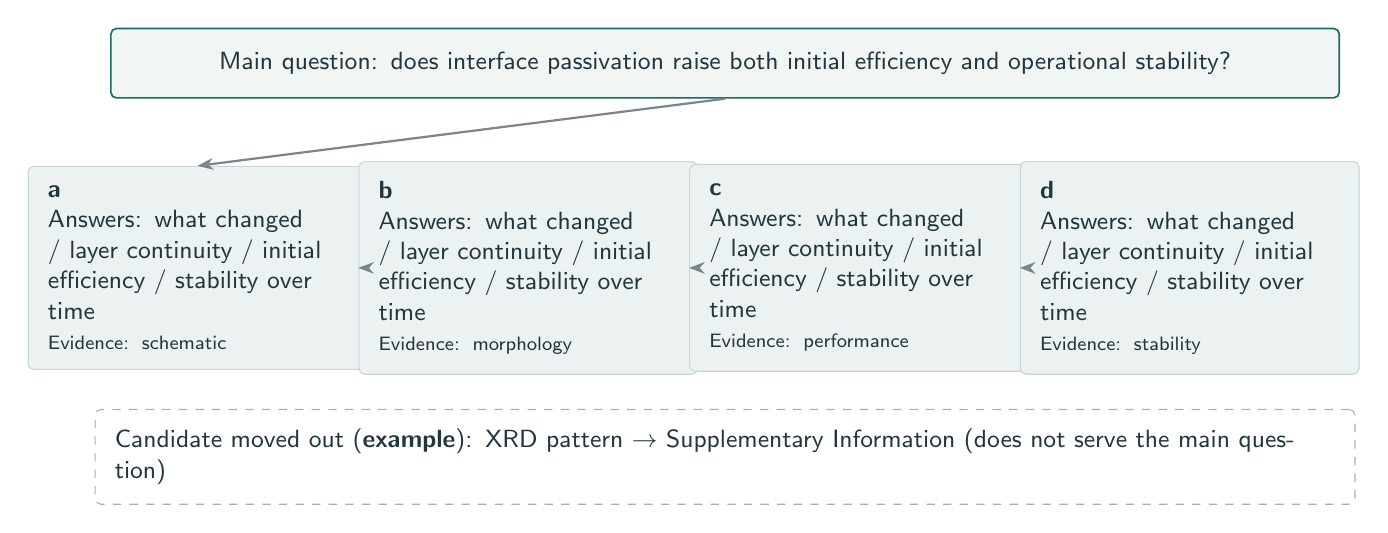
\begin{tikzpicture}[
  x=1mm, y=1mm,
  font=\sffamily\small,
  text=BookInk,
  mainbox/.style={
    draw=BookTeal, line width=0.6pt, rounded corners=2pt,
    fill=BookPale, align=center, text width=150mm, inner sep=3mm,
  },
  explain/.style={
    draw=BookRule, fill=BookRule!35, rounded corners=2pt,
    align=left, text width=38mm, inner sep=2.5mm, minimum height=18mm,
  },
  moved/.style={
    draw=BookInk!40, dashed, rounded corners=2pt,
    align=left, text width=155mm, inner sep=2.5mm,
  },
]
  \node[mainbox] (q) at (87, 58)
    {Main question: does interface passivation raise both initial efficiency and operational stability?};
  \foreach \i/\x/\t in {
    a/20/schematic, b/62/morphology, c/104/performance, d/146/stability} {
    \node[explain] (\i) at (\x, 32) {
      \textbf{\i}\par
      Answers: what changed / layer continuity / initial efficiency / stability over time\par
      \scriptsize Evidence: \t
    };
  }
  \draw[-{Stealth[length=2mm]}, BookInk!60, thick] (q.south) -- (a.north);
  \draw[-{Stealth[length=2mm]}, BookInk!60] (a.east) -- (b.west);
  \draw[-{Stealth[length=2mm]}, BookInk!60] (b.east) -- (c.west);
  \draw[-{Stealth[length=2mm]}, BookInk!60] (c.east) -- (d.west);
  \node[moved] at (87, 8) {
    Candidate moved out (\textbf{example}): XRD pattern $\rightarrow$ Supplementary Information (does not serve the main question)
  };
\end{tikzpicture}
}
\caption{How the panels of Figure 2 share the argument. Each panel answers one sub-question of the main question; a candidate panel that does not serve the main question moves to the Supplementary Information.}\label{fig:ch09-01}
\end{figure}

Defining each panel's role immediately settles the layout sequence: \textbf{reading order must mirror argumentative order}. Readers of scientific journals scan multi-panel figures from left to right and from top to bottom (Jambor et al., 2021). Placing the two explanatory panels (\textbf{a} and \textbf{b}) across the top row to establish ``what the device is,'' and placing the two quantitative data panels (\textbf{c} and \textbf{d}) across the bottom row to demonstrate ``how the device performs,'' creates a natural visual path. As the reader's eye moves along $\textbf{a} \rightarrow \textbf{b} \rightarrow \textbf{c} \rightarrow \textbf{d}$, it follows the exact logical progression from structural design to layer morphology, initial efficiency, and long-term stability, without backtracking across the page.

An explicit argument map also gives a clear criterion for pruning clutter: \textbf{any candidate panel that does not directly advance the main question belongs in the Supplementary Information}. The test is simple: \textbf{If we remove this panel, can Figure 2 still answer its main question completely?} As shown by the dashed box at the bottom of Figure~\ref{fig:ch09-01}, suppose the author also has an X-ray diffraction (XRD) pattern confirming that the annealed film crystallized into the expected perovskite phase without impurity peaks (shown here purely as a planning example; our simulated dataset contains no XRD data). That spectrum answers ``Did the film form the target crystal phase?''---a routine synthesis check rather than direct evidence of whether interface passivation raises efficiency and lifetime. Moving the XRD pattern to the Supplementary Information frees up space so the four core panels remain legible.

At this stage, an author can send the main question and candidate panel list to an AI assistant to help structure sub-questions and flag off-topic panels:

\begin{Prompt}
I am planning Figure 2 (double-column width, 174 mm) for a perovskite solar cell paper.
Main question: Does passivation at the perovskite/hole-transport-layer interface
simultaneously improve initial efficiency and operational stability?
Candidate panels: (1) layered device schematic; (2) cross-sectional morphology image;
(3) control vs. modified J-V curves; (4) 1000 h normalized PCE stability curves;
(5) thin-film XRD phase-confirmation pattern.
List the sub-question and evidence type for each panel, identify which candidate does
not directly serve the main question and should move to Supplementary Information, and
propose a left-to-right, top-to-bottom reading order for the remaining panels.
\end{Prompt}

AI can quickly organize candidate roles from your prompt and point out that item (5) addresses baseline phase purity rather than the interface passivation claim. Yet the boundary of responsibility remains strict: \textbf{AI cannot judge whether your experimental evidence is scientifically sufficient, nor can it decide which measurements may be ethically omitted}. Deciding which results belong in the main text and which routine characterizations move to the supplement rests entirely with the authors.

\section{Plan the grid at final size}

Once the panel roster and reading sequence are locked, the second step is to design the layout grid directly at the \textbf{final print dimensions of the target journal}, rather than plotting individual charts at large default sizes and shrinking them later to fit a multi-panel canvas.

Why is ``plotting big and shrinking later'' the primary cause of illegible text in composite figures? Consider the arithmetic. When you open Python's Matplotlib without specifying dimensions, the default canvas is $8 \times 6\ \text{in}$ ($203.2 \times 152.4\ \text{mm}$) with $10\ \text{pt}$ text. Viewed alone on a laptop screen, that chart looks well proportioned. In print and PDF layouts, however, journal column widths are fixed physical constants. Across most Springer and Cell Press titles (and in the corresponding presets of \scidraw{}'s multi-panel tool), a single column is roughly $84\text{--}85\ \text{mm}$ and a double-column spread is $174\ \text{mm}$; across Nature Portfolio journals, a single column is $89\ \text{mm}$ and a double-column spread is $183\ \text{mm}$.

When two panels sit side by side across a $174\ \text{mm}$ canvas with a $6\ \text{mm}$ column gap, each cell gets $(174 - 6) / 2 = 84\ \text{mm}$ of width. Scaling a $203.2\ \text{mm}$-wide graphic down into an $84\ \text{mm}$ cell multiplies every dimension by:
\[
s = \frac{84\ \text{mm}}{203.2\ \text{mm}} \approx 0.413
\]
Original $10\ \text{pt}$ tick numbers and axis titles shrink to roughly $4.1\text{--}4.5\ \text{pt}$, while $0.8\ \text{pt}$ axis lines thin down to $0.33\ \text{pt}$ hairlines.

Publishers enforce strict minimum type sizes \textbf{at final print width}. Nature Portfolio's figure guide specifies $5\text{--}7\ \text{pt}$ for standard text and $8\ \text{pt}$ bold lowercase for panel letters. Under a more conservative cross-journal standard---such as the $8\ \text{pt}$ minimum preset for Springer-style layouts, which also ensures comfortable screen reading during peer review---all ticks, axis titles, and callouts should be at least $8\ \text{pt}$, with panel letters at $10\ \text{pt}$ bold (always verify the target journal's current author instructions before plotting and before submission). Under either standard, $4.5\ \text{pt}$ text is unreadable.

The only reliable fix is to \textbf{define the millimeter dimensions of the composite canvas and grid cells first, and plot every data panel directly at its final cell dimensions (dividing millimeters by $25.4$ to get inches) so that the assembly scale factor is exactly $1.0$}. If you later reformat for a $183\ \text{mm}$ journal with $6\text{--}7\ \text{pt}$ text, simply update the width and font constants in your script and re-run, rather than stretching raster panels by hand.

Grid planning must also respect the \textbf{natural aspect ratio} of each panel's content. A device schematic, a cross-sectional image, and a line plot have different proportions. Figure~\ref{fig:ch09-02} compares two candidate grids at the $174\ \text{mm}$ print width.

\begin{figure}[htbp]\centering
\resizebox{0.84\linewidth}{!}{% FIG ch09-02 layout wireframes (English)
\begin{tikzpicture}[
  x=1mm, y=1mm,
  font=\sffamily\footnotesize,
  text=BookInk,
  frame/.style={draw=BookInk!70, line width=0.5pt},
  cell/.style={draw=BookRule, fill=BookPale!50, line width=0.3pt},
  bad/.style={pattern=north east lines, pattern color=BookInk!25},
]
  \node[anchor=west, font=\bfseries] at (0, 125) {Option A (equal 2$\times$2 cells)};
  \draw[frame] (0, 68) rectangle (174, 122);
  \node[anchor=south] at (87, 122) {174 mm};
  \foreach \x/\y/\w/\h in {0/68/84/53, 90/68/84/53, 0/10/84/53, 90/10/84/53} {
    \draw[cell] (\x,\y) rectangle (\x+\w,\y+\h);
  }
  \draw[bad] (90,68) rectangle (174,121);
  \node[anchor=west, text=BookTeal] at (92, 95) {stretch req.\ \ding{55}};
  \node[anchor=west, align=left, text width=84mm] at (0, 4) {
    Pros: simple grid. Issue: panel b must be stretched to fill its cell.
  };

  \node[anchor=west, font=\bfseries] at (0, 248) {Option B (chosen)};
  \draw[frame] (0, 186) rectangle (174, 240);
  \draw[cell] (0,214) rectangle (84,264);
  \draw[cell] (90,214) rectangle (174,264);
  \draw[cell] (0,154) rectangle (84,210);
  \draw[cell] (90,154) rectangle (174,210);
  \draw[BookTeal, dashed, line width=0.4pt] (12,154) -- (12,210);
  \draw[BookTeal, dashed, line width=0.4pt] (102,154) -- (102,210);
  \node[text=BookTeal, font=\scriptsize] at (57,152) {align};
  \node[text=BookTeal, font=\scriptsize] at (147,152) {align};
  \node[anchor=west, align=left, text width=90mm] at (0, 178) {
    Top row 84$\times$50 mm; bottom 84$\times$56 mm; 6 mm column gap, 8 mm row gap.
  };
  \node[anchor=west, align=left, text width=84mm] at (0, 168) {
    Pros: keeps aspect ratio of b; aligns c/d axes. Issue: sizes must be planned upfront.
  };
\end{tikzpicture}
}
\caption{Two grid options compared at final print width. Option A uses equal cells, so the cross-section would have to be stretched to fill its cell; option B sizes rows by content and aligns the axes of the two data panels. Dimensions in mm.}\label{fig:ch09-02}
\end{figure}

In \textbf{Option A (equal $2 \times 2$ cells)}, shown in the lower half of Figure~\ref{fig:ch09-02}, a $174 \times 114\ \text{mm}$ canvas is split into four equal $84 \times 53\ \text{mm}$ cells. However, Panel \textbf{a} has a $\sim 16:10$ aspect ratio and needs 35\% of its width on the right for seven layer labels; Panel \textbf{b} has a strict $3:2$ aspect ratio; and Panels \textbf{c} and \textbf{d} need outer margins for axis titles. Forcing Panel \textbf{b} to fill an equal cell in Option A (the hatched area) requires non-uniform vertical stretching, distorting both layer thickness ratios and columnar grain morphology.

In \textbf{Option B (row heights matched to content, chosen here)}, shown in the upper half of Figure~\ref{fig:ch09-02}, the top explanatory row (\textbf{a}, \textbf{b}) gets $84 \times 50\ \text{mm}$ per cell with native aspect ratios preserved by clean whitespace, while the bottom data row (\textbf{c}, \textbf{d}) gets $84 \times 56\ \text{mm}$. A $6\ \text{mm}$ column gap separates left and right panels, an $8\ \text{mm}$ row gap separates explanatory and data rows, and the coordinate spine boxes of \textbf{c} and \textbf{d} are strictly aligned (dashed teal lines).

\section{Make panels speak one language}

When panels originate in different tools---here, Panels \textbf{a} and \textbf{b} start as model-generated base images while Panels \textbf{c} and \textbf{d} come from Python scripts---a draft easily looks like a patchwork clipped from four separate papers. Making heterogeneous panels read as a single cohesive figure requires five shared rules of visual grammar.

\textbf{First, unify the typeface to one sans-serif family and compress the hierarchy of font sizes and stroke weights.}
Use a single sans-serif family (Helvetica, Arial, or TeX Gyre Heros) across the entire figure, never mixing serif schematic labels with sans-serif data ticks. Restrict font sizes to two tiers: $10\ \text{pt}$ bold for the panel letters (\textbf{a}--\textbf{d}), and $8\ \text{pt}$ for all other text (axis titles, ticks, curve callouts, layer names, and provenance badges). Keep stroke weights uniform as well: $0.6\ \text{pt}$ for axis spines and ticks, $1.2\ \text{pt}$ for data curves, $1.0\ \text{pt}$ light-grey dotted lines for benchmarks, and $0.5\ \text{pt}$ pale grey rules for horizontal grid lines.

\textbf{Second, maintain consistent color semantics across every panel.}
Color in a multi-panel figure acts as a visual pronoun for a specific experimental group (Wong, 2011; Crameri et al., 2020). Once assigned in Panel \textbf{a}, it must keep that meaning everywhere. In our case study, interface passivation is the central variable: in Panel \textbf{a}, the ultra-thin passivation layer above the perovskite absorber is drawn in teal (\texttt{\#1B7F86}), and its label ``Passivation layer'' uses the same teal ink. In Panels \textbf{c} and \textbf{d}, the modified device curves and direct labels continue to use \texttt{\#1B7F86}, while the unpassivated control group uses neutral dark grey (\texttt{\#6E6E6E}). Having learned ``teal = passivated'' in Panel \textbf{a}, the reader decodes Panels \textbf{c} and \textbf{d} without searching for a legend key.

\textbf{Third, combine color with line style for greyscale and color-vision accessibility.}
Hue alone is fragile: dark grey (\texttt{\#6E6E6E}) and deep teal (\texttt{\#1B7F86}) have nearly identical luminance, so two solid lines become indistinguishable when printed in black and white, and readers with color-vision deficiencies likewise need non-color cues (Machado et al., 2009). We therefore add \textbf{redundant line-style encoding} (Figure~\ref{fig:ch09-05}): modified devices use a \textbf{solid teal line}, control devices use a \textbf{dashed grey line} ($4:2$ dash-to-gap), and the 80\% threshold in Panel \textbf{d} uses a \textbf{light-grey (\texttt{\#9A9A9A}) dotted line} ($1:3$). Solid, dashed, and dotted curves remain unmistakable even on a monochrome photocopy.

\begin{figure}[htbp]\centering
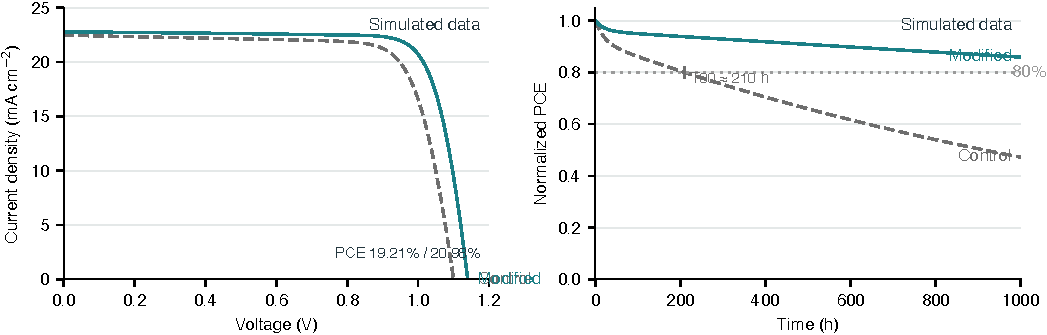
\includegraphics[width=\linewidth]{figures/ch09/ch09-05-data-panels-en.pdf}
\caption{The two data panels drawn at final size ($84 \times 56\ \text{mm}$ each). (c) Simulated $J\text{--}V$ curves for control (grey, dashed) and modified (teal, solid) devices. (d) Normalized PCE over time; the dotted line marks 80\%. The groups differ in both color and line style, so they remain distinguishable in greyscale. Curves were generated with a single-diode model and prescribed decay functions; simulated teaching data. Notice the lower-right corner of the left plot: when direct labels are anchored mechanically to the final data point of each curve, the two traces dropping to zero at $V_{\text{oc}}$ cause ``Control'' and ``Modified'' to collide with each other and with the terminal tick label, an issue corrected in the final assembly (Figure~\ref{fig:ch09-07}).}\label{fig:ch09-05}
\end{figure}

\textbf{Fourth, replace boxed legends with direct curve labels---and audit the rendered plot for geometric text collisions.}
For two-curve plots, replacing an enclosed legend box with color-matched text labels beside the traces removes eye jumps between legend and data.

Yet direct labeling cannot be coded blindly as ``place the label at the last point \texttt{(x[-1], y[-1])}.'' Inspecting the actual image in Figure~\ref{fig:ch09-05} shows the collision caused by automatic endpoint anchoring: in the left plot (Panel \textbf{c}), both $J\text{--}V$ curves drop steeply on the right to intersect the horizontal axis ($J = 0$) at their open-circuit voltages ($1.100\ \text{V}$ and $1.140\ \text{V}$). Binding labels to the curve endpoints causes ``Control'' and ``Modified'' to pile directly on top of each other over the \texttt{1.2} tick mark at the lower right, while the ``PCE 19.21\% / 20.98\%'' summary string is sliced through by the dashed control curve. In the right plot (Panel \textbf{d}), ``Modified,'' ``80\%,'' and ``Control'' crowd the right ends of their trajectories at $1000\ \text{h}$, and ``$\text{T80} \approx 210\ \text{h}$'' sits directly across the dashed curve.

Thus, \textbf{direct labels must be placed intentionally inside open white bands beside the curves and checked at 200\% zoom}. In our final assembly (Figure~\ref{fig:ch09-07}), we move ``Modified'' and ``Control'' in Panel \textbf{c} to the open band left of the steep drop---at $(0.96\ \text{V},\ 15.5\ \text{mA cm}^{-2})$ and $(1.00\ \text{V},\ 5.0\ \text{mA cm}^{-2})$---and move the PCE summary to the lower-left corner $(0.03,\ 0.04)$; in Panel \textbf{d}, we place the labels in the open corridors above their curves with semi-transparent white backing pads, eliminating all overlaps.

\textbf{Fifth, standardize units and embed provenance declarations inside every panel.}
Delete standalone subplot titles (``J-V curve,'' ``Stability test'') that repeat the caption; unify units to $\text{V}$, $\text{mA cm}^{-2}$, and $\text{h}$ with proper subscripts ($\mathrm{SnO_2}$); and place ``Not to scale'' (\textbf{a}), ``Model-generated illustration, not a micrograph'' (\textbf{b}), and ``Simulated data'' (\textbf{c}, \textbf{d}) inside the frames so provenance stays attached if a panel is reused in slides or posters.

\section{Alignment, labels, and white space}

When assembling four panels onto a shared canvas, visual polish depends on three geometric details: coordinate spine alignment, panel lettering, and purposeful whitespace.

\textbf{First: align coordinate axis spine boxes, not outer image bounding boxes.}
Panel \textbf{c}'s vertical axis has two-digit integers (\texttt{0--25}) and a title with superscripts, whereas Panel \textbf{d}'s vertical axis has decimals (\texttt{0.0--1.0}). If both plots are exported with tight bounding boxes (\texttt{bbox\_inches='tight'}) and aligned by their left image edges, their differing label widths push the inner coordinate rectangles out of alignment.

Because readers track the drawn axis spines rather than invisible text margins, composite assembly should avoid elastic auto-layout (\texttt{tight\_layout}) and \textbf{fix exact millimeter coordinates for every panel frame on the canvas}. On the $174.0 \times 116.0\ \text{mm}$ canvas of our final figure (Figure~\ref{fig:ch09-07}), we reserve $13.0\ \text{mm}$ on the left for vertical axis labels and lock the left column (Panel \textbf{a} frame and Panel \textbf{c} spine box) to $x = 13.0\text{--}82.0\ \text{mm}$ (width $69.0\ \text{mm}$). After a $6.0\ \text{mm}$ column gap and a $13.0\ \text{mm}$ label corridor, the right column (Panel \textbf{b} frame and Panel \textbf{d} spine box) is locked to $x = 101.0\text{--}170.0\ \text{mm}$ (width $69.0\ \text{mm}$), leaving a $4.0\ \text{mm}$ right margin with terminal ticks ``1.2'' and ``1000'' right-aligned inward. Both bottom spine boxes sit at $y = 11.0\text{--}57.0\ \text{mm}$ (height $46.0\ \text{mm}$), verified by script assertions (\texttt{assert}).

\textbf{Second: keep panel letters uniform in style, position, and baseline in an outer white corridor.}
Four rules govern panel letters:
\begin{enumerate}
\item \textbf{Single style:} Follow journal conventions uniformly ($10\ \text{pt}$ TeX Gyre Heros Bold lowercase \textbf{a}--\textbf{d}, without parentheses or periods).
\item \textbf{Aligned left edges and row baselines:} Align \textbf{a}, \textbf{c} at $x = 13.0\ \text{mm}$ and \textbf{b}, \textbf{d} at $x = 101.0\ \text{mm}$; align upper-row (\textbf{a}, \textbf{b}) and lower-row (\textbf{c}, \textbf{d}) letters on shared horizontal baselines $1.0\ \text{mm}$ above each panel frame's top edge.
\item \textbf{Top safety strip:} Reserve $5.0\ \text{mm}$ of white space at the top of the canvas so upper-row letters are never clipped.
\item \textbf{Outside dark interiors:} Place letters in the outer white corridor so they never vanish against Panel \textbf{b}'s dark upper background.
\end{enumerate}

\textbf{Third: use whitespace to signal grouping, and preserve native image aspect ratios.}
Between-group spacing should exceed within-group spacing: we set the horizontal column gap to $6.0\ \text{mm}$ and the vertical gap between the upper explanatory row (\textbf{a}, \textbf{b}) and lower data row (\textbf{c}, \textbf{d}) to $8.0\ \text{mm}$. Image panels must never use non-uniform stretching (\texttt{aspect='auto'}): at $69.0\ \text{mm}$ column width, Panel \textbf{a} ($1586 \times 992\ \text{px}$) is naturally $43.2\ \text{mm}$ tall and Panel \textbf{b} ($1536 \times 1024\ \text{px}$) is $46.0\ \text{mm}$ tall. Aligning their top edges at $y = 111.0\ \text{mm}$ leaves a natural $2.8\ \text{mm}$ white strip below Panel \textbf{a} for the incident-light and ``Not to scale'' labels.

\section{Case: Figure 2 from cluttered to review-ready}

We now walk through the complete assembly of Figure 2 for our planar perovskite solar cell case study---from material inventory and drawing brief to base-image auditing, initial v1 diagnosis, v2 revision, and reproduction in \scidraw{} (sharing the simulated dataset used in Chapters 12 and 13).

\subsection*{Step 1: Inventorying materials and simulation parameters}

The teaching scenario compares planar regular (n-i-p) control devices against devices with an interfacial passivation layer between the perovskite absorber and hole-transport layer. From bottom to top, the stack is glass / FTO / $\text{SnO}_2$ (schematic thickness $\sim 30\ \text{nm}$) / perovskite ($\sim 500\ \text{nm}$) / passivation layer (modified group only, ultra-thin) / spiro-OMeTAD ($\sim 200\ \text{nm}$) / Au ($\sim 80\ \text{nm}$), illuminated through the glass. We do not specify a perovskite composition or passivating molecule, nor do we report real device data.

Among the four inputs, M1 (Panel \textbf{a} structure schematic) and M2 (Panel \textbf{b} SEM-style cross-sectional illustration) are generated as text-free base images; M3 (Panel \textbf{c} $J\text{--}V$ curves) is solved by bisection in $0.5\ \text{mV}$ steps from the single-diode equation $J = J_{\text{L}} - J_0[\exp((V + J R_{\text{s}})/(n V_{\text{T}})) - 1] - (V + J R_{\text{s}})/R_{\text{sh}}$ at $25\ ^\circ\text{C}$ ($V_{\text{T}} = 0.025693\ \text{V}$) under AM1.5G ($100\ \text{mW cm}^{-2}$) for a single scan direction without hysteresis; and M4 (Panel \textbf{d} stability over $0\text{--}1000\ \text{h}$ in $10\ \text{h}$ steps) follows the bi-exponential decay $y(t) = [1 - b(1 - e^{-t/20})]e^{-t/\tau}$ ($b = 0.08, \tau = 1500\ \text{h}$ for control; $b = 0.04, \tau = 9000\ \text{h}$ for modified). Each group has one representative simulated curve; parameters and metrics appear in Table~\ref{tab:ch09-sim}.

\begin{table}[htbp]\centering\footnotesize
\setlength{\tabcolsep}{3.5pt}
\renewcommand{\arraystretch}{1.15}
\caption{Single-diode simulation parameters and derived photovoltaic metrics for panels c and d (simulated teaching data).}\label{tab:ch09-sim}
\begin{tabularx}{\linewidth}{@{}lcccYY@{}}
\toprule
\textbf{Group} & $J_{\text{L}}$ / target $V_{\text{oc}}$ & $n$ & $R_{\text{s}}$ / $R_{\text{sh}}$ ($\Omega\cdot\text{cm}^2$) & \textbf{Derived $J_{\text{sc}}$ / $V_{\text{oc}}$ / FF} & \textbf{Derived PCE and $T_{80}$} \\
\midrule
Control & $22.5\ \text{mA cm}^{-2}$ / $1.10\ \text{V}$ & 1.6 & $2.5$ / $1500$ & $22.46\ \text{mA cm}^{-2}$ / $1.100\ \text{V}$ / $0.777$ & $19.21\%$; $T_{80} = 210\ \text{h}$ \\
Modified & $22.8\ \text{mA cm}^{-2}$ / $1.14\ \text{V}$ & 1.5 & $2.0$ / $3000$ & $22.78\ \text{mA cm}^{-2}$ / $1.140\ \text{V}$ / $0.808$ & $20.98\%$; $T_{80} > 1000\ \text{h}$ \\
\bottomrule
\end{tabularx}
\end{table}

\begin{BookNote}
\textbf{Why not use an open-licensed real SEM micrograph for panel b?} Open-access literature provides CC BY 4.0 perovskite SEM images, such as Figure 6 of Burkitt, Searle, and Watson (2018) (top-view Jeol JSM-7800F SEM images of spin- and slot-die-coated films with $10\ \mu\text{m}$ and $1\ \mu\text{m}$ scale bars). However, that study uses a \textbf{mesoporous $\text{TiO}_2$ scaffold with $\text{MAPbI}_{3-x}\text{Cl}_x$ and $\sim 7\%$ stabilized efficiency}, unrelated to our planar $\text{SnO}_2$ stack and simulated metrics. Placing it into Figure 2 would falsely imply that the morphology and performance curves came from the same devices---violating Chapter 8's rule against presenting images from different samples as one source. Thus Panel \textbf{b} uses an explicitly labeled model-generated illustration; in real research, it must be an actual SEM image of the same device batch with raw files preserved.
\end{BookNote}

\subsection*{Step 2: The multi-panel drawing brief}

The complete drawing brief is written and saved in our own document; at layout time we choose ``Multi-panel figure'' in the \scidraw{} figure workflow guide (\sdtool{figure-workflow}) and follow the route into the panel tool, working from this brief:

\begin{Prompt}
[Use and audience] Paper Figure 2, double-column width 174 mm, height <= 120 mm;
audience is perovskite photovoltaics peers. Prepared to Springer-style standards:
minimum text >= 8 pt (verify current author instructions before submission).
[Main question] Does interface passivation raise both initial efficiency and stability?
[Panel roles]
a Device structure (modified stack; passivation highlighted) -- answers "what changed".
b Cross-section morphology -- answers "layer continuity". In this book, a model-generated
  illustration labeled in-panel "Model-generated illustration, not a micrograph".
c J-V curves (control, modified) -- answers "initial efficiency gain and driving parameter".
d Normalized PCE over time (control, modified, 0.8 line) -- answers "stability gain".
Reading order a->b->c->d: structure and morphology first, performance second.
[Layout] Top row a, b (explanatory); bottom row c, d (data); c and d axis boxes aligned
with identical height; 6 mm column gap; panel letters top-left, bold lowercase, shared baseline.
[Unified style] Single sans-serif font; ticks, axis titles, callouts 8 pt; panel letters
10 pt bold; axis lines 0.6 pt, data lines 1.2 pt; control #6E6E6E dashed, modified #1B7F86
solid; passivation layer in a also #1B7F86; 0.8 reference line light-grey dotted; direct
labels without legend boxes; units written V, mA cm^-2, h.
[Invariants] All numbers in c, d from the sim-perovskite dataset; aspect ratio of b locked;
in-panel notes "Simulated data" on c, d and "Not to scale" on a.
[Deliverables & acceptance] Vector PDF (selectable text) + high-res raster; processing log;
author-completed legend. At 174 mm (100% scale): min text >= 8 pt; c/d spines aligned;
greyscale distinguishable; b unstretched; all in-panel provenance notes visible.
\end{Prompt}

\subsection*{Step 3: Generating base images for panels a and b and auditing model deviations}

Panel \textbf{a}'s text-free base image is generated with the following English prompt (reserving the right 35\% of the canvas for labels):

\begin{Prompt}
A clean, flat, two-dimensional scientific schematic of a planar thin-film solar
cell shown as a stack of horizontal layers in side view with a slight sense of
thickness. From bottom to top: a thick pale blue-grey translucent glass slab;
a thin light grey conductive layer; a very thin off-white layer; a thicker
dark reddish-brown absorber layer; an extremely thin teal layer (hex #1B7F86)
directly on top of the absorber; a pale yellow layer; and a thin gold metal
layer on top. Three simple upward-pointing light arrows below the glass,
pale yellow with grey outline. The stack occupies the left 65% of the canvas;
leave the right 35% empty white space for labels added later.
White background, vector illustration style, no gradients, no shadows,
no 3D rendering, no glow, no texture. Layers are not to scale but each layer is
clearly separated by a thin dark grey outline.
Absolutely no text, no letters, no numbers, no labels, no symbols, no scale bar.
Aspect ratio 16:10.
\end{Prompt}

Running the prompt three times yields $1586 \times 992\ \text{px}$ PNGs (aspect ratio $1.599:1$, $-0.08\%$ from $16:10$), all showing the seven layers in order, three upward light arrows, and a text-free white background. However, candidate 2 draws the teal passivation layer too thick ($\sim 29\ \text{px}$), and candidate 3 shifts the teal toward a lighter cyan (median \texttt{\#298F97}) while widening the right margin to 38.5\%. Candidate 1 leaves 35\% whitespace on the right and renders a thin teal layer whose measured median color (\texttt{\#20868D}) is within $5\text{--}7$ RGB units of \texttt{\#1B7F86}, so we select it as the main base image. Two minor deviations remain: subtle shading and fine grain appear inside the layers despite \texttt{no gradients, no texture}, and the front glass layer ($\sim 148\ \text{px}$) is slightly thinner than the absorber layer ($\sim 158\ \text{px}$). We overlay the seven layer names with leader lines and add ``Not to scale'' at the bottom right (Figure~\ref{fig:ch09-03}).

\begin{figure}[htbp]\centering
\begin{tikzpicture}
\node[anchor=south west,inner sep=0] (img) at (0,0) {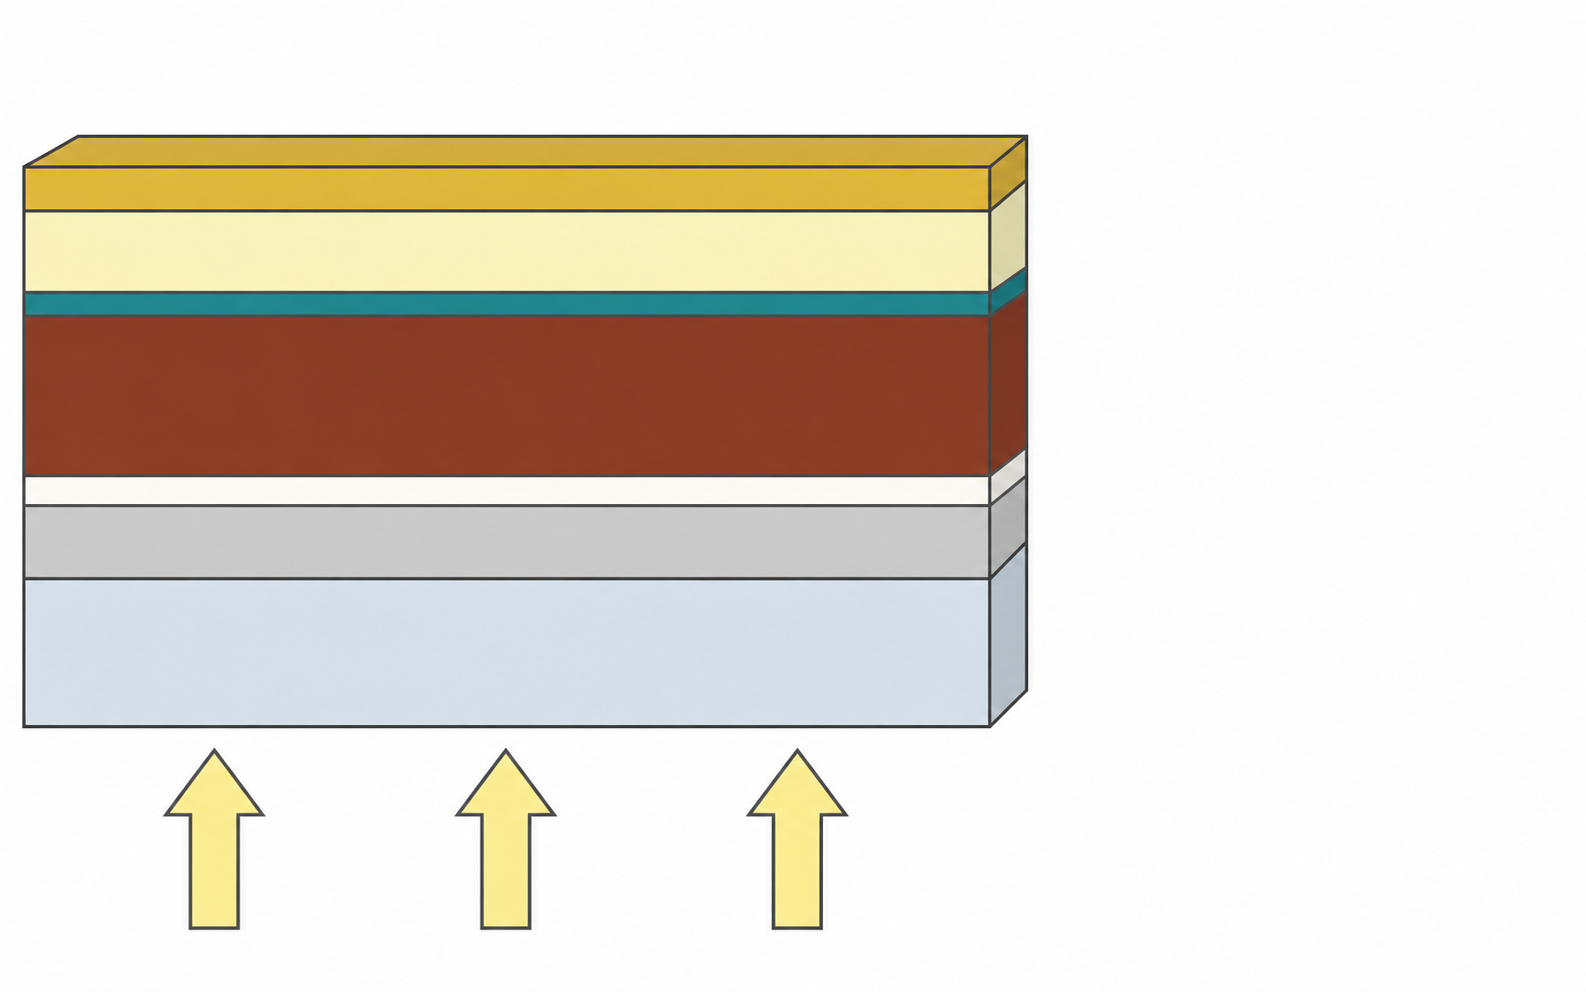
\includegraphics[width=0.86\linewidth]{figures/ch09/ch09-03-device-structure-base.png}};
\begin{scope}[x={(img.south east)},y={(img.north west)},font=\sffamily\footnotesize]
  \draw[BookInk!65,thin] (0.60,0.83) -- (0.69,0.86);
  \draw[BookInk!65,thin] (0.60,0.75) -- (0.69,0.76);
  \draw[BookTeal,thin] (0.60,0.698) -- (0.69,0.67);
  \draw[BookInk!65,thin] (0.60,0.60) -- (0.69,0.56);
  \draw[BookInk!65,thin] (0.60,0.505) -- (0.69,0.45);
  \draw[BookInk!65,thin] (0.60,0.45) -- (0.69,0.39);
  \draw[BookInk!65,thin] (0.60,0.33) -- (0.69,0.25);
  \node[anchor=west] at (0.70,0.86) {Au};
  \node[anchor=west] at (0.70,0.76) {spiro-OMeTAD};
  \node[anchor=west,text=BookTeal,font=\sffamily\footnotesize\bfseries] at (0.70,0.67) {Passivation layer};
  \node[anchor=west] at (0.70,0.56) {Perovskite};
  \node[anchor=west] at (0.70,0.45) {$\mathrm{SnO_2}$};
  \node[anchor=west] at (0.70,0.39) {FTO};
  \node[anchor=west] at (0.70,0.25) {Glass};
  \node[anchor=west] at (0.30,0.05) {Light};
  \node[anchor=south east,text=BookInk!80] at (0.98,0.02) {Not to scale};
\end{scope}
\end{tikzpicture}
\caption{Schematic of the modified device (panel a). The base image was drawn by an image-generation model and the layer names were added afterwards. The passivation layer uses the same teal as the ``modified'' series in the data panels. Layers are not to scale.}\label{fig:ch09-03}
\end{figure}

Panel \textbf{b}'s base image is generated with the following prompt (explicitly forbidding scale bars and instrument banners because a model-generated illustration has no physical scale):

\begin{Prompt}
A grayscale illustration in the visual style of a cross-sectional scanning
electron micrograph of a layered thin film, for use as a clearly labelled
teaching illustration. From bottom to top: a thick smooth featureless layer
filling the bottom third; a very thin slightly brighter layer; a thicker layer
made of densely packed columnar grains with visible grain boundaries; a
smoother amorphous layer; and a thin bright layer at the top. Dark background
above the top layer. Slightly irregular fractured edge. Even illumination,
moderate contrast. No scale bar, no data bar, no measurement marks, no text,
no letters, no numbers, no labels, no watermark. Aspect ratio 3:2.
\end{Prompt}

All three runs produce $1536 \times 1024\ \text{px}$ images (exact $3:2$) with five clear strata and no pseudo-text or fake scale bars. Candidate 1 has overly deep inter-grain crevices; candidate 2 expands the bottom layer to $42\%\text{--}43\%$ of the height with a steep downward slope at the top right. Candidate 3 (chosen as our main image) shows natural top fracture contours and clear grain boundaries, though the bottom layer still occupies $38\%\text{--}39\%$ of the height (above one-third) with faint graininess, and the RGB channels differ by up to $10$ units per pixel rather than being strictly identical. We overlay a white badge in the lower-left corner reading ``Model-generated illustration, not a micrograph'' (Figure~\ref{fig:ch09-04}).

\begin{figure}[htbp]\centering
\begin{tikzpicture}
\node[anchor=south west,inner sep=0] (img) at (0,0) {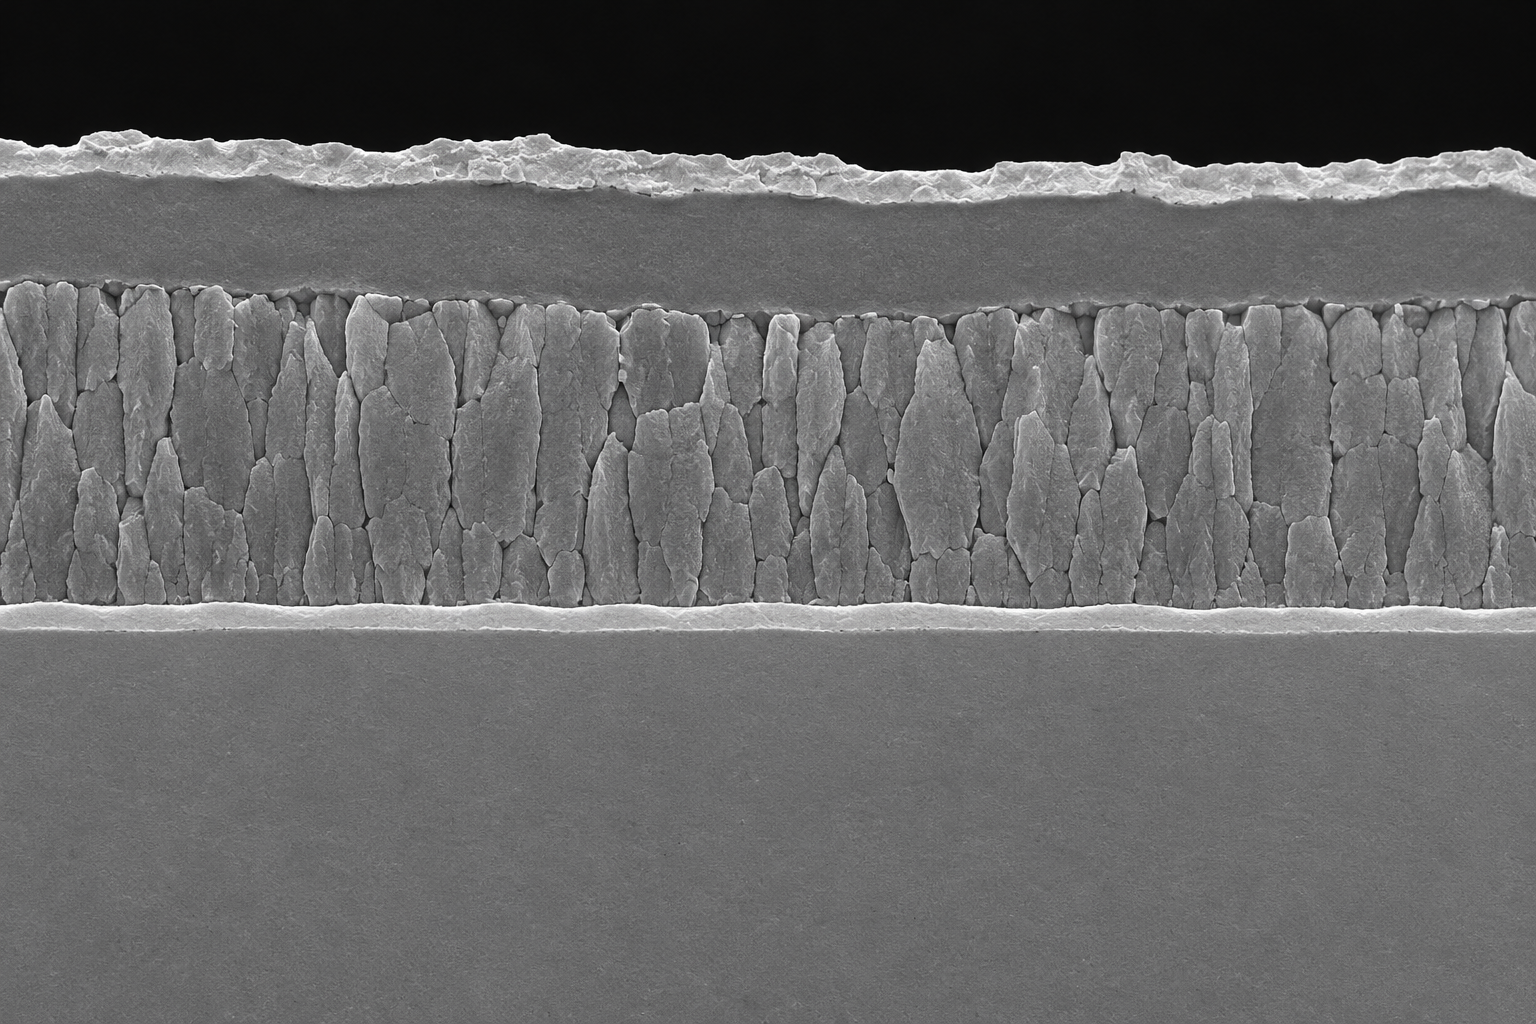
\includegraphics[width=0.78\linewidth]{figures/ch09/ch09-04-sem-like-illustration-base.png}};
\begin{scope}[x={(img.south east)},y={(img.north west)}]
  \node[anchor=south west,fill=white,fill opacity=0.90,text opacity=1,text=black,font=\sffamily\footnotesize,inner sep=2.5pt] at (0.02,0.03) {Model-generated illustration, not a micrograph};
\end{scope}
\end{tikzpicture}
\caption{Model-generated illustration of the cross-section (panel b). It was drawn by an image-generation model, is not a micrograph and has no physical scale; it only indicates layer order and layout. In a real paper this panel must be an actual SEM image of the same batch of devices, with the raw image and processing record kept (Chapter 8).}\label{fig:ch09-04}
\end{figure}

\subsection*{Step 4: Auditing the ten defects in the initial assembly (v1) and writing the revision order}

Figure~\ref{fig:ch09-06} reproduces the initial uncoordinated assembly (v1), with red badges 1--10 marking ten concrete defects on the canvas:

\begin{figure}[htbp]\centering
\resizebox{\linewidth}{!}{%
\begin{tikzpicture}
\definecolor{ChNineBad}{HTML}{C0392B}
\node[anchor=south west,inner sep=0] (img) at (0,0) {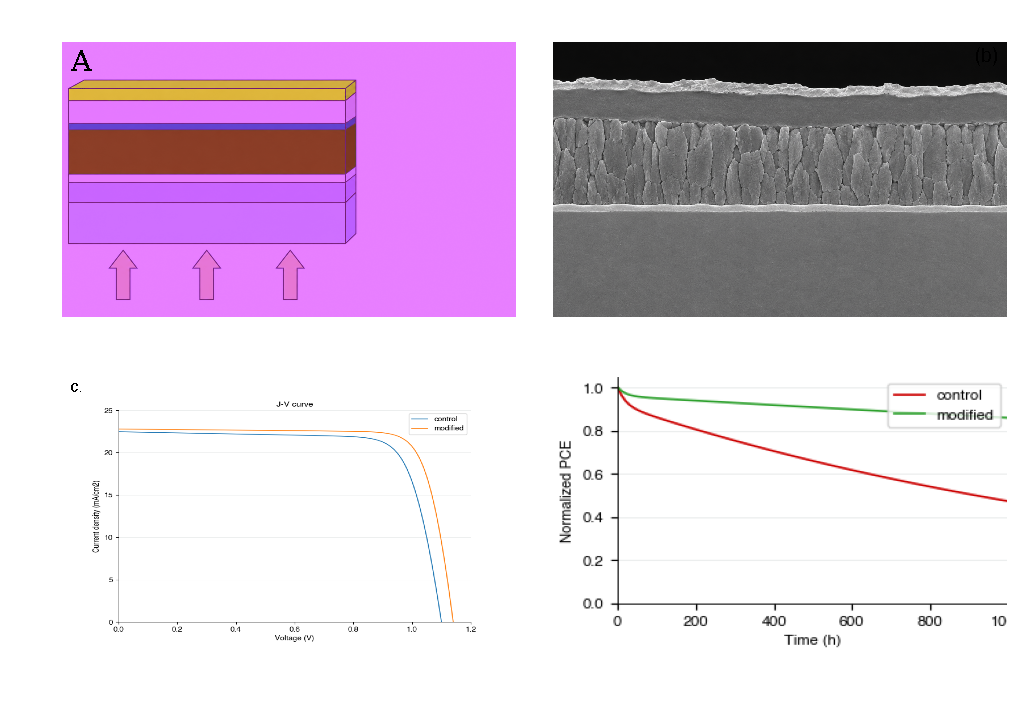
\includegraphics[width=\linewidth]{figures/ch09/ch09-06-assembly-v1-en.pdf}};
\begin{scope}[x={(img.south east)},y={(img.north west)}]
  \tikzset{
    badnum/.style={draw=white,line width=0.7pt,fill=ChNineBad,text=white,circle,font=\sffamily\bfseries\scriptsize,inner sep=1pt,minimum size=4.0mm},
    badtxt/.style={fill=white,fill opacity=0.88,text opacity=1,text=ChNineBad!90!black,font=\sffamily\scriptsize\bfseries,inner sep=1.2pt,rounded corners=1pt}
  }
  \node[badnum] (b1) at (0.03,0.95) {1};
  \node[badtxt,anchor=west] at (b1.east) {Mixed panel letters};
  \node[badnum] (b2) at (0.62,0.30) {2};
  \node[badtxt,anchor=west] at (b2.east) {Mismatched font sizes};
  \node[badnum] (b3) at (0.20,0.70) {3};
  \node[badtxt,anchor=west] at (b3.east) {Inconsistent color semantics};
  \node[badnum] (b4) at (0.85,0.20) {4};
  \node[badtxt,anchor=east] at (b4.west) {Indistinguishable in greyscale};
  \node[badnum] (b5) at (0.75,0.40) {5};
  \node[badtxt,anchor=west] at (b5.east) {Legend box overlaps curve};
  \node[badnum] (b6) at (0.50,0.08) {6};
  \node[badtxt,anchor=west] at (b6.east) {Misaligned axis boxes};
  \node[badnum] (b7) at (0.75,0.75) {7};
  \node[badtxt,anchor=west] at (b7.east) {Panel b stretched};
  \node[badnum] (b8) at (0.50,0.52) {8};
  \node[badtxt,anchor=west] at (b8.east) {Uneven panel spacing};
  \node[badnum] (b9) at (0.92,0.92) {9};
  \node[badtxt,anchor=east] at (b9.west) {Missing provenance notes};
  \node[badnum] (b10) at (0.30,0.45) {10};
  \node[badtxt,anchor=west] at (b10.east) {Redundant subplot titles};
\end{scope}
\end{tikzpicture}}
\caption{First assembly (v1, a deliberately reproduced counter-example). Numbers 1--10 mark the problems discussed in the text. Panel b is a model-generated illustration, not a micrograph, and panels c and d show simulated data; this version omits those in-panel notes, which is problem 9.}\label{fig:ch09-06}
\end{figure}

\begin{enumerate}
\item \textbf{Mixed and missing panel letters (1):} Panel \textbf{a} uses a $14\ \text{pt}$ serif ``A''; Panel \textbf{b} has a $9\ \text{pt}$ ``(b)'' nearly lost in the dark upper-right background; Panel \textbf{c} uses ``c.''; and Panel \textbf{d} omits its letter.
\item \textbf{Mismatched font sizes and clipped ticks (2):} Panel \textbf{c} was plotted at $8 \times 6\ \text{in}$ ($10\ \text{pt}$) and scaled down, shrinking its ticks to $\sim 4.5\ \text{pt}$; Panel \textbf{d} was plotted at $84 \times 56\ \text{mm}$ ($8\ \text{pt}$), and its rightmost tick ``1000'' is clipped to ``10'' at the border.
\item \textbf{Inconsistent color semantics (3):} A hue shift in Panel \textbf{a} turned the passivation layer deep purple and tinted the background magenta-violet; Panel \textbf{c} uses default blue/orange; and Panel \textbf{d} uses red/green.
\item \textbf{Indistinguishable in greyscale (4):} Both data panels use solid lines for both groups, and Panel \textbf{d}'s red/green pairing is unfriendly to color-blind readers.
\item \textbf{Legend box overlapping data (5):} Both data plots use boxed legends, and Panel \textbf{d}'s legend sits directly over the green modified curve.
\item \textbf{Misaligned axis spine boxes (6):} The coordinate spine boxes of \textbf{c} and \textbf{d} are offset by $1.4\ \text{mm}$ on the left edge and $3.2\ \text{mm}$ on the bottom edge.
\item \textbf{Stretched image panel (7):} Panel \textbf{b} uses \texttt{aspect='auto'} to match Panel \textbf{a}'s height, vertically distorting the grains.
\item \textbf{Uneven panel spacing (8):} Irregular \texttt{GridSpec} gaps obscure the grouping hierarchy.
\item \textbf{Missing provenance notes and benchmark line (9):} Panels lack ``Not to scale,'' ``Model-generated illustration,'' and ``Simulated data'' badges, Panel \textbf{a} has no layer names, and Panel \textbf{d} omits the $0.8$ line.
\item \textbf{Redundant subplot titles and unformatted units (10):} Panels \textbf{c} and \textbf{d} have top titles (``J-V curve,'' ``Stability test'') duplicating the legend, and Panel \textbf{c} writes \texttt{mA/cm2}.
\end{enumerate}

We address all ten issues with a structured revision order:

\begin{Prompt}
Revision order (v1 -> v2)
1. Unify panel letters to 10 pt bold sans-serif lowercase a-d outside each frame's top-left
   corner on shared row baselines (reserve a 5 mm white safety strip at the canvas top).
2. Redraw c and d directly on the 174 x 116 mm master canvas at 8 pt text (scale factor 1.0).
3. Unify color semantics: control #6E6E6E dashed, modified #1B7F86 solid; restore the clean
   white-background base image in a and set the "Passivation layer" label in #1B7F86.
4. Remove boxed legends; place color-matched direct labels ("Control", "Modified") in open
   white bands beside the curves so no text touches a data trace or tick mark.
5. Lock horizontal frame spans: left column (a, c) x = 13-82 mm; right column (b, d)
   x = 101-170 mm; c and d spine boxes at y = 11-57 mm (46 mm tall); right-align terminal
   ticks "1.2" and "1000" inside the 4 mm right margin.
6. Place a and b at native aspect ratios (69 x 43.2 mm and 69 x 46.0 mm), top-aligned at y = 111 mm.
7. Set inter-column gap to 6 mm (plus 13 mm y-axis corridor) and inter-row gap to 8 mm.
8. Add "Simulated data" to c and d, "Model-generated illustration, not a micrograph" to b,
   layer labels + "Not to scale" to a, and the 0.8 dotted line + "80%" + "T80 ~ 210 h" to d.
9. Remove subplot titles; standardize units to V, mA cm^-2, and h.
10. Export vector PDF (pdf.fonttype = 42) and 300 dpi PNG; log panel dimensions and scale factors.
\end{Prompt}

\subsection*{Step 5: Revised assembly (v2) and reproducing the layout in SciDraw AI}

The revised composite figure (v2) appears in Figure~\ref{fig:ch09-07}. To assemble the same four pre-rendered panels in the \scidraw{} multi-panel tool (\sdtool{multi-panel-figure-maker}), follow three checkpoints:

\begin{figure}[htbp]\centering
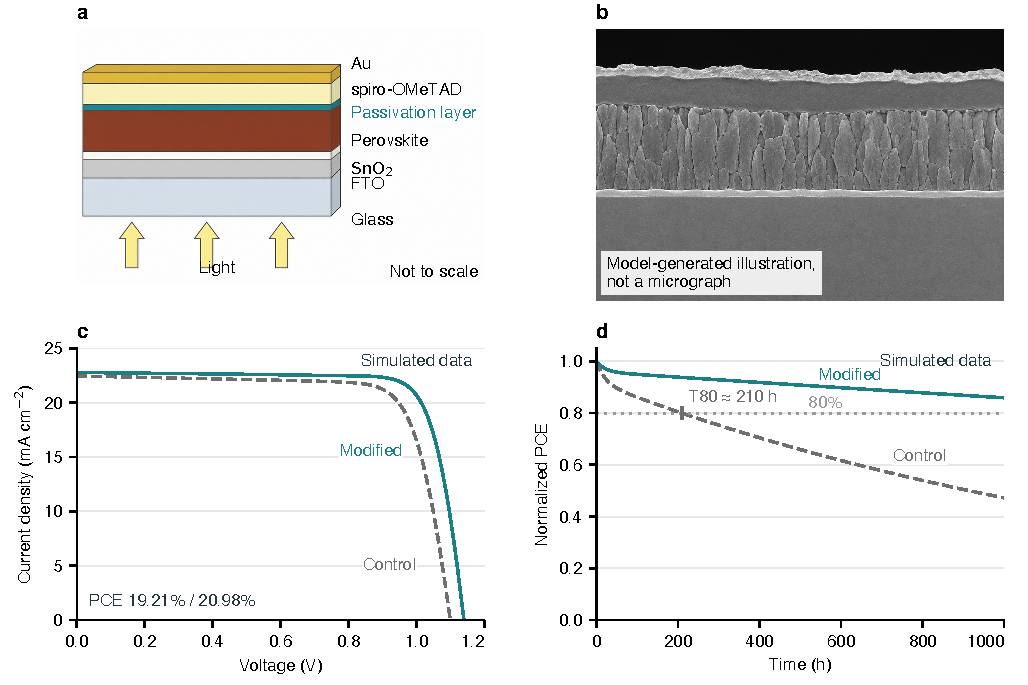
\includegraphics[width=\linewidth]{figures/ch09/ch09-07-assembly-final-en.pdf}
\caption{Revised assembly (v2). \textbf{Fig.~2 | Effect of interface passivation on the initial performance and operational stability of perovskite solar cells (simulated teaching data).} \textbf{a}, Schematic of the modified device (glass/FTO/$\text{SnO}_2$/perovskite/passivation layer/spiro-OMeTAD/Au; light enters through the glass); the control device has no passivation layer; layer thicknesses are not to scale. \textbf{b}, Illustration of the cross-section drawn by an image-generation model; \textbf{not a micrograph}, shown only to indicate layer order. \textbf{c}, $J\text{--}V$ curves of control (grey, dashed) and modified (teal, solid) devices simulated with a single-diode model (AM1.5G, $100\ \text{mW cm}^{-2}$, one scan direction, no hysteresis modeled); PCE 19.21\% (control) and 20.98\% (modified). \textbf{d}, Normalized PCE over time under simulated conditions (continuous 1-sun illumination, maximum-power-point tracking, $\text{N}_2$, about $25\ ^\circ\text{C}$); the dotted line marks 80\% of the initial value; $T_{80}$ is about $210\ \text{h}$ for the control, and the modified device stays above 80\% for $1{,}000\ \text{h}$. Panels c and d show one simulated curve per group, not a distribution across devices, and no statistical test was performed. Simulation parameters and script are provided in the book repository.}\label{fig:ch09-07}
\end{figure}

\begin{enumerate}
\item \textbf{File handoff and journal presets:} Tools do not transfer images automatically; upload the labeled PNGs for \textbf{a} and \textbf{b} and final-size PNGs for \textbf{c} and \textbf{d} into \texttt{/multi-panel-\allowbreak figure-\allowbreak maker} (saved in browser local storage). Choose the Springer or Cell $174\ \text{mm}$ double-column preset and a $2 \times 2$ grid with auto-numbering. Because numbering follows the preset (lowercase \textbf{a} for Springer, uppercase \textbf{A} for Cell), verify the target journal's author instructions before submission.
\item \textbf{Export bundle and tool boundaries:} Export the ZIP containing TIFF, PNG, PDF, PPTX, and the processing record. In PPTX, panel bitmaps and outer letters are separate objects, but text inside panel bitmaps is not editable; the tool does not auto-plan layouts, edit internal panel text, or vectorize bitmaps.
\item \textbf{Reading the processing record for font size and resolution:} Check the logged cell dimensions and scale factors. If Panel \textbf{c} was plotted at $84\ \text{mm}$ ($8\ \text{pt}$) but placed at $80\ \text{mm}$ (scale factor $0.952$), its effective font size drops to $8 \times 80 / 84 \approx 7.6\ \text{pt}$, requiring re-export from the script at the exact cell width. Bitmap resolution equals source pixel width divided by placed width in inches: at $69.0\ \text{mm}$ ($2.717\ \text{in}$), Panel \textbf{a} ($1586\ \text{px}$) and Panel \textbf{b} ($1536\ \text{px}$) reach $1586 / 2.717 \approx 584\ \text{ppi}$ and $1536 / 2.717 \approx 565\ \text{ppi}$, well above $300\ \text{ppi}$.
\end{enumerate}

\section{Legends: AI drafts, the author completes}

A complete multi-panel legend contains five parts: an opening title sentence, panel-by-panel descriptions (defining visual encodings), key experimental or simulation conditions, sample sizes and statistical methods, and data provenance declarations.

When you upload the composite PNG to the \scidraw{} legend assistant (\sdtool{figure-legend}), the tool reads only the image pixels and outputs a 40--120 word descriptive draft, typically along the lines of: ``Device structure, cross-sectional morphology, and photovoltaic performance of perovskite solar cells. (a) Schematic of the layered device architecture. (b) Cross-sectional image of the device stack. (c) $J\text{--}V$ curves of control and modified devices. (d) Normalized PCE as a function of time.''

By design, \sdtool{figure-legend} never fabricates sample sizes, $p$-values, statistical tests, test conditions, or chemical formulas invisible in the image. The author must separate \textbf{what is visible in the pixels} from \textbf{what the author must supply} (Figure~\ref{fig:ch09-08}):

\begin{figure}[htbp]\centering
\resizebox{\linewidth}{!}{% FIG ch09-08 legend drafting (English)
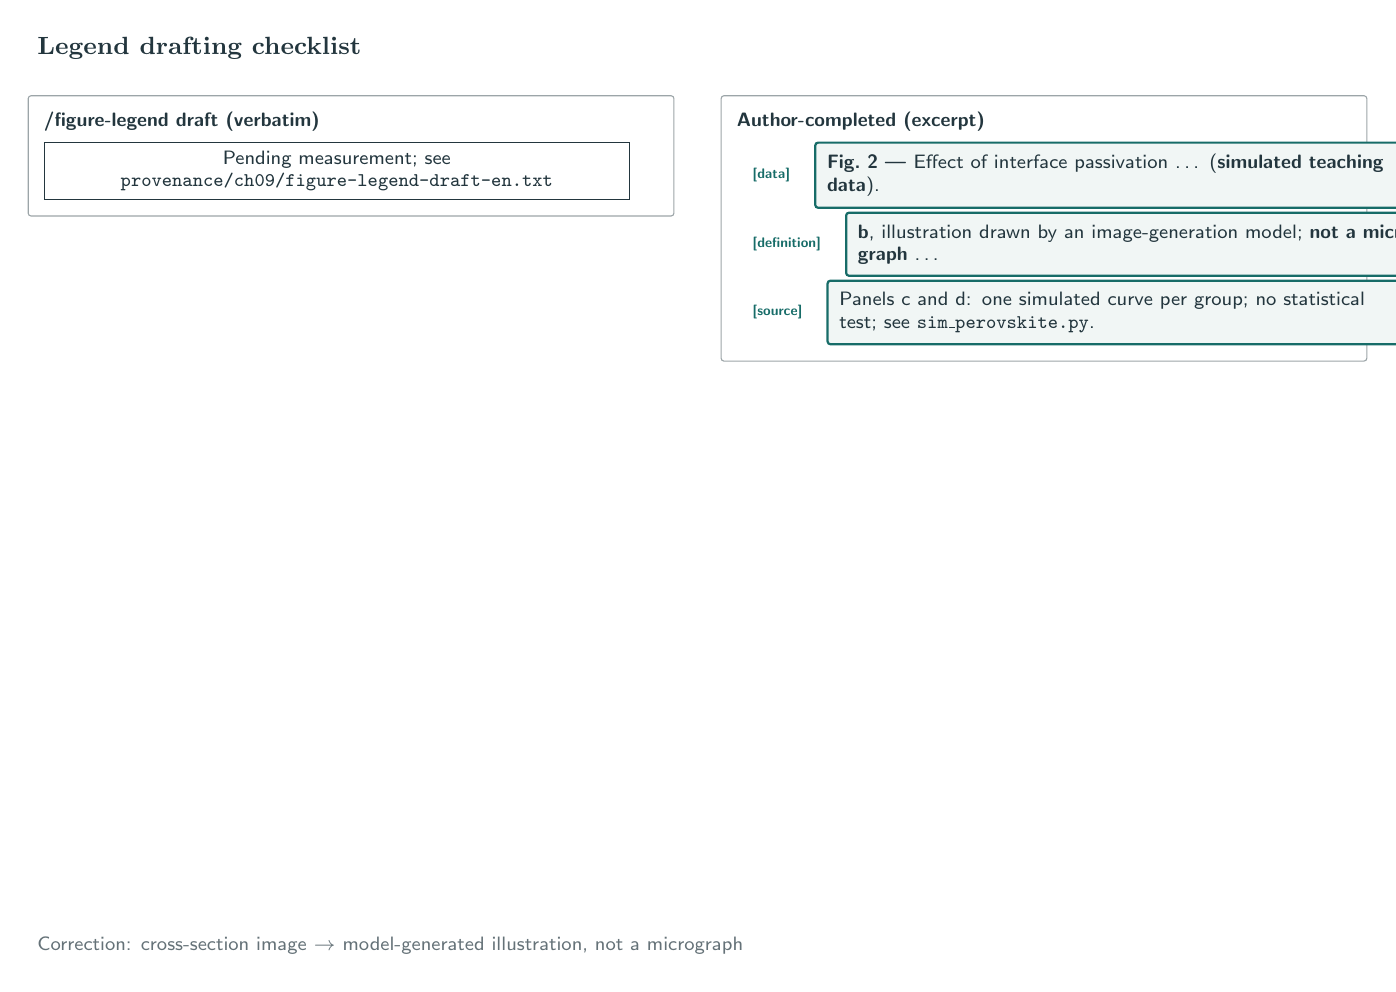
\begin{tikzpicture}[
  x=1mm, y=1mm,
  font=\sffamily\scriptsize,
  text=BookInk,
  col/.style={draw=BookInk!45, line width=0.4pt, rounded corners=1pt, inner sep=2mm, align=justify, text width=78mm},
  hi/.style={fill=BookPale, draw=BookTeal, line width=0.8pt, rounded corners=1pt, inner sep=1.5mm},
  tag/.style={font=\tiny\bfseries, text=BookTeal, anchor=east},
]
  \node[font=\small\bfseries, anchor=west] at (0, 118) {Legend drafting checklist};
  \node[col, anchor=north west] at (0, 112) {
    \textbf{/figure-legend draft (verbatim)}\par\vspace{1mm}
    \fbox{\parbox[t]{72mm}{\centering Pending measurement; see \texttt{provenance/ch09/figure-legend-draft-en.txt}}}
  };
  \node[col, anchor=north west] at (88, 112) {
    \textbf{Author-completed (excerpt)}\par\vspace{1mm}
    \tikz{\node[hi, text width=72mm, anchor=west] at (0,0) {
      \textbf{Fig.~2 |} Effect of interface passivation \ldots\ (\textbf{simulated teaching data}).
    }; \node[tag] at (-1,0) {[data]};}\par
    \tikz{\node[hi, text width=72mm, anchor=west] at (0,0) {
      \textbf{b}, illustration drawn by an image-generation model; \textbf{not a micrograph} \ldots
    }; \node[tag] at (-1,0) {[definition]};}\par
    \tikz{\node[hi, text width=72mm, anchor=west] at (0,0) {
      Panels c and d: one simulated curve per group; no statistical test; see \texttt{sim\_perovskite.py}.
    }; \node[tag] at (-1,0) {[source]};}
  };
  \node[anchor=west, text=BookInk!70] at (0, 4) {
    Correction: \sout{cross-section image} $\rightarrow$ model-generated illustration, not a micrograph
  };
\end{tikzpicture}
}
\caption{AI drafts the legend; the author completes it. Left: the draft produced by \sdtool{figure-legend} from the image (verbatim). Right: the completed legend; highlighted text is information that cannot be seen in the image and must come from the author.}\label{fig:ch09-08}
\end{figure}

\begin{itemize}
\item \textbf{Correcting visual misclassifications:} The draft may call Panel \textbf{b} a ``cross-sectional image / SEM image''; replace this with ``Illustration of the cross-section drawn by an image-generation model; not a micrograph, shown only to indicate layer order.''
\item \textbf{Supplying five categories of context:} (1) \textbf{[Data nature]} Simulated teaching data, layers not to scale, not a micrograph; (2) \textbf{[Devices and conditions]} Seven-layer stack and illumination side, single-diode model (AM1.5G, $100\ \text{mW cm}^{-2}$, one scan direction, no hysteresis---real perovskite cells exhibit hysteresis and require reporting scan direction and rate per Snaith et al., 2014), and stability conditions (continuous 1-sun illumination, MPP tracking, $\text{N}_2$, $\sim 25\ ^\circ\text{C}$; verify any ISOS-L-1 protocol label against Khenkin et al., 2020); (3) \textbf{[Samples and statistics]} PCE $19.21\%$ vs.\ $20.98\%$, stating that each curve is a single simulated trajectory with no device distribution or statistical test; (4) \textbf{[Definitions]} Dotted line at 80\% of initial efficiency, control $T_{80} \approx 210\ \text{h}$, modified $> 1000\ \text{h}$; (5) \textbf{[Source]} Simulation parameters and script location (see full caption in Figure~\ref{fig:ch09-07}).
\end{itemize}

For empirical research papers, authors can fill in the following template from their lab records:

\begin{BookNote}
\textbf{Empirical paper legend template:} \textbf{c}, Representative $J\text{--}V$ curves (reverse scan, [scan rate] $\text{mV s}^{-1}$, active area [area] $\text{cm}^2$, aperture mask [with/without]); inset table gives photovoltaic parameters (mean $\pm$ s.d.) for $n =$ [devices] devices across [batches] independent batches. \textbf{d}, Normalized PCE of $n =$ [devices] unencapsulated devices per group under [atmosphere] at [temperature] $^\circ\text{C}$; shaded bands show [s.d.\ / s.e.m.\ / range]; $T_{80}$ is defined as [time to first drop below 80\% / fitted value]. Statistical test: [method], [$P$ value].
\end{BookNote}

Before delivery, combine \sdtool{figure-checker} with script assertions to complete the eight-point verification in Table~\ref{tab:ch09-verify}.

\begin{table}[htbp]\centering\footnotesize
\setlength{\tabcolsep}{3pt}
\renewcommand{\arraystretch}{1.15}
\caption{Eight-point pre-delivery verification of the final composite figure (Figure~\ref{fig:ch09-07}).}\label{tab:ch09-verify}
\begin{tabularx}{\linewidth}{@{}>{\raggedright\arraybackslash}p{26mm}YY@{}}
\toprule
\textbf{Check item} & \textbf{Verification method} & \textbf{Measured result on final figure} \\
\midrule
Numerical consistency & Script assertions comparing summary CSV metrics against plot and caption numbers & PCE ($19.21\%$ / $20.98\%$) and $T_{80}$ ($210\ \text{h}$ / $>1000\ \text{h}$) match identically \\
100\% print font size & Check PDF font properties at $174\ \text{mm}$ width or measure cap height ($8\ \text{pt} \approx 2.0\ \text{mm}$) & Panel letters $10\ \text{pt}$ bold; all other text $8\ \text{pt}$ with zero border clipping \\
Spine box alignment & Assert millimeter coordinates of all four frames via \texttt{ax.get\_position()} & \textbf{a}/\textbf{c} locked to $13\text{--}82\ \text{mm}$; \textbf{b}/\textbf{d} locked to $101\text{--}170\ \text{mm}$; \textbf{c}/\textbf{d} bottom at $11\ \text{mm}$ \\
Image aspect ratio & Compare placed frame ratios against source PNG pixel dimensions & Panel \textbf{a} ($69.0 \times 43.2\ \text{mm}$) and Panel \textbf{b} ($69.0 \times 46.0\ \text{mm}$) error $< 0.1\%$ \\
Greyscale \& CVD safety & Greyscale conversion and Machado (2009) CVD simulation / \sdtool{figure-checker} & Grey dashed, teal solid, and light-grey dotted lines remain separable \\
In-panel declarations & Visual audit of all four panel interiors at 100\% scale & ``Not to scale,'' ``Model-generated illustration, not a micrograph,'' and ``Simulated data'' visible \\
Scale factor \& ppi & Check processing log scale factor and compute source pixels $\div$ placed inches & \textbf{c}, \textbf{d} scale factor $1.0$; \textbf{a} $\sim 584\ \text{ppi}$, \textbf{b} $\sim 565\ \text{ppi}$ \\
Legend traceability & Cross-check every number and condition in the caption against data and script settings & All numbers trace to data files and simulation parameters; no unsupported claims \\
\bottomrule
\end{tabularx}
\end{table}

\section{What AI Can and Cannot Do at This Stage}

Table~\ref{tab:ch09-01} summarizes the responsibilities of AI, deterministic tools, and the author across multi-panel assembly and legend preparation.

\begin{table}[htbp]\centering\footnotesize
\setlength{\tabcolsep}{3pt}
\renewcommand{\arraystretch}{1.15}
\caption{What AI can do, what AI cannot do, and what the author must verify when assembling multi-panel figures.}\label{tab:ch09-01}
\begin{tabularx}{\linewidth}{@{}>{\raggedright\arraybackslash}p{20mm}YYY@{}}
\toprule
\textbf{Stage} & \textbf{What AI can do} & \textbf{What AI cannot do} & \textbf{What the author must verify} \\
\midrule
Panel roles & List candidate panel roles and reading orders from a brief; flag panels unrelated to the main question & Judge whether evidence suffices to support the conclusion, or decide which data may be omitted & The sub-question each panel answers; destination of removed panels (Supplementary Information) \\
Grid planning & Convert journal widths into cell sizes; write \texttt{gridspec} or fixed-axis scripts & Weigh scientific importance to allocate area (the multi-panel tool does not do AI layout planning) & Final dimensions, preserved aspect ratios, and grouping whitespace \\
Schematic panels & Generate text-free base images showing layer order or stylized morphology & Guarantee accurate layer sequence, realistic proportions, or empirical morphological evidence & Layer count and sequence, shared color semantics, and ``not to scale / model-generated'' labels \\
Data panels & Write plotting scripts to spec; unify \texttt{rcParams} & Select or alter data values, or invent error bands that do not exist & Values match data files; font size meets specs at final width; greyscale separability \\
Layout \& export & \scidraw{} multi-panel tool: grids, row/column spans, auto-numbering, journal presets, processing logs, TIFF/PNG/PDF/PPTX & Edit text inside panel bitmaps, unify fonts across rasterized panels, or turn bitmaps into editable vectors & Scale factors and effective ppi in the processing record; numbering style matches journal rules \\
Figure legend & \sdtool{figure-legend}: draft descriptions of visually observable features & Write sample sizes, batches, test conditions, statistical methods, or data nature (never fabricated by design) & Supply $n$, conditions, statistics, definitions ($T_{80}$), and sources; remove misclassifications (e.g., SEM) \\
Technical check & \sdtool{figure-checker}: check format, resolution, greyscale, and color-vision risks & Audit scientific conclusions or statistical choices & Full scientific verification beyond technical checks \\
\bottomrule
\end{tabularx}
\end{table}

\section{Chapter Checklist}

\begin{itemize}
\item The main question of the composite figure is written down, every panel has a clear sub-question or evidential role, and unrelated panels have been moved out.
\item The canvas is set to the target journal's final width ($174\ \text{mm}$ in this example) and stays within height limits.
\item Data panels are exported directly at their final cell dimensions with an assembly scale factor of $1.0$ (or effective font sizes have been calculated from the scale factor).
\item One sans-serif font family is used throughout; minimum text meets journal rules; panel letters share a uniform style, size, and position.
\item Coordinate axis spine boxes of side-by-side data panels are aligned; inter-panel gaps are uniform, with between-group whitespace larger than within-group whitespace.
\item Each experimental group keeps the same color across all panels; line styles or direct labels provide non-color redundancy; greyscale and color-vision checks pass.
\item Image panels preserve their native aspect ratios without stretching.
\item Declarations for simulated data, model-generated illustrations, and not-to-scale schematics are written \textbf{inside the panels} as well as in the legend.
\item The legend includes a title sentence, panel-by-panel descriptions, sample sizes and replicates, test conditions, statistical methods and error definitions, threshold definitions (such as $T_{80}$), and data/code sources.
\item Processing records, scripts, raw data, and exported composite files are archived together, with file handoffs between scripts and layout tools recorded.
\end{itemize}

\section{Exercises}

\begin{enumerate}
\item \textbf{Panel argument mapping (pen and paper).} Take one of your recent multi-panel figures, write down its main question and the sub-question for each panel, and identify one panel that does not directly answer the main question. Explain whether it should stay, be merged, or move to the Supplementary Information.
\item \textbf{Final-size check (script).} Using this chapter's data-panel plotting script, export Panel \textbf{c} both at $\text{figsize}=(8,6)\ \text{in}$ and at $84 \times 56\ \text{mm}$, place each into an $84\ \text{mm}$-wide cell, and calculate the effective printed tick-label font size in both cases; then change the control curve to a solid line matching the modified curve, convert to greyscale, and record whether the groups can be distinguished.
\item \textbf{Hands-on practice with \scidraw{}.} Import the four panel PNGs provided with this chapter into \texttt{/multi-panel-\allowbreak figure-\allowbreak maker}, select the Springer and Cell $174\ \text{mm}$ presets in turn, and compare their numbering styles; export the ZIP archive, read Panel \textbf{c}'s scale factor from the processing record, and compute its effective font size. Next, upload the exported PNG to \sdtool{figure-legend}, save the verbatim draft, and complete the legend across the categories in Section 9.6. \emph{Extension:} Read Figure 6 of Burkitt et al.\ (2018) (CC BY 4.0, real SEM figure), list the information a real SEM panel must provide inside the figure and in the legend (instrument, viewing angle, scale bar, sample stack, and processing), and explain why it cannot be placed into Figure 2 of this chapter.
\end{enumerate}

\section*{References}

\begin{itemize}
\item Burkitt D, Searle J, Watson T. Perovskite solar cells in N-I-P structure with four slot-die-coated layers. \textit{Royal Society Open Science}. 2018;5(5):172158. doi:10.1098/\allowbreak rsos.172158
\item Crameri F, Shephard GE, Heron PJ. The misuse of colour in science communication. \textit{Nature Communications}. 2020;11:5444. doi:10.1038/\allowbreak s41467-020-19160-7
\item Jambor H, Antonietti A, Alicea B, et al. Creating clear and informative image-based figures for scientific publications. \textit{PLOS Biology}. 2021;19(3):e3001161. doi:10.1371/\allowbreak journal.pbio.3001161
\item Khenkin MV, Katz EA, Abate A, et al. Consensus statement for stability assessment and reporting for perovskite photovoltaics based on ISOS procedures. \textit{Nature Energy}. 2020;5(1):35--49. doi:10.1038/\allowbreak s41560-019-0529-5
\item Kojima A, Teshima K, Shirai Y, Miyasaka T. Organometal halide perovskites as visible-light sensitizers for photovoltaic cells. \textit{Journal of the American Chemical Society}. 2009;131(17):6050--6051. doi:10.1021/\allowbreak ja809598r
\item Machado GM, Oliveira MM, Fernandes LAF. A physiologically-based model for simulation of color vision deficiency. \textit{IEEE Transactions on Visualization and Computer Graphics}. 2009;15(6):1291--1298. doi:10.1109/\allowbreak TVCG.2009.113
\item Nature Portfolio. Preparing figures -- our specifications. \url{https://research-figure-guide.nature.com/figures/preparing-figures-our-specifications/} (accessed 2026-10-29).
\item Rougier NP, Droettboom M, Bourne PE. Ten simple rules for better figures. \textit{PLoS Computational Biology}. 2014;10(9):e1003833. doi:10.1371/\allowbreak journal.pcbi.1003833
\item Snaith HJ, Abate A, Ball JM, et al. Anomalous hysteresis in perovskite solar cells. \textit{The Journal of Physical Chemistry Letters}. 2014;5(9):1511--1515. doi:10.1021/\allowbreak jz500113x
\item Wong B. Points of view: Color blindness. \textit{Nature Methods}. 2011;8(6):441. doi:10.1038/\allowbreak nmeth.1618
\end{itemize}

% TODO: provenance/ch09/figure-legend-draft-en.txt has not yet been generated (the left column of figures/ch09/ch09-08-legend-drafting-en.tex currently shows a "Pending measurement" placeholder box).
% TODO: standalone pre-overlaid bitmaps figures/ch09/ch09-03-device-structure-en.png and figures/ch09/ch09-04-sem-like-illustration-en.png have not been generated separately (this chapter displays the base images with TikZ overlays as specified by book-spec Section 6, and the composite figure ch09-07 embeds the overlays directly).
% TODO: figures/ch09/ch09-05-data-panels-en.pdf was exported before the direct-label coordinate adjustment in ch09_plot_utils.py (the "Control" and "Modified" labels at the lower right still overlap at the curve endpoints); re-running scripts/ch09_panels.py will synchronize it with ch09-07.

\chapter{Graphical Abstracts: One Image for One Contribution}

Zhou, a doctoral student working in satellite remote sensing and deep learning, has just received an acceptance letter for her manuscript. At the bottom of the email, the editorial office adds one final requirement: within a week, submit a graphical abstract to appear in the online table of contents (TOC) and at the top of the article page. To Zhou, the task sounds trivial. She opens her manuscript folder, selects Figure 1---an encoder--decoder network diagram with skip connections, channel dimensions, attention blocks, and a loss equation---scales it down proportionally, and uploads the exported image.

Two days later, the technical editor returns the file with a two-sentence note: ``This diagram shows the internal architecture of your network, not the contribution of your study; and when scaled to table-of-contents size, the text is illegible.''

Many authors asked for a graphical abstract for the first time step into the same trap: either they shrink a method diagram (Figure 1) from the paper, or they cram four or five result plots into one frame like a miniature poster. Specialists in the exact sub-field do not need the thumbnail, while readers browsing the table of contents from neighboring areas cannot tell in five seconds what problem the paper addresses or what it found. This chapter shows how to design a single image that communicates one research contribution and its essential boundary conditions clearly and conservatively under strict size and viewing-time constraints.

\section{What a Graphical Abstract Must Answer}

A graphical abstract is a single figure placed in an online table of contents, search listings, and the top of an article page. Within the three to eight seconds a reader spends scanning a table of contents, the image should answer three linked questions---\textbf{``Does this paper address a problem relevant to my work? How did the authors approach it? What bounded finding did they establish?''}

To accomplish that job, a graphical abstract needs to convey only a three-part chain: \textbf{Question --- Method --- Finding and Limits}. It does not catalog kernel sizes layer by layer, list hyperparameters or secondary ablations, or reproduce statistical plots with error bars and significance asterisks.

Before sketching a layout, distinguish the graphical abstract from three other visual formats that are often confused with it:

\begin{center}\footnotesize
\setlength{\tabcolsep}{3pt}
\renewcommand{\arraystretch}{1.15}
\begin{tabularx}{\linewidth}{@{}>{\raggedright\arraybackslash}p{23mm}>{\raggedright\arraybackslash}p{25mm}YY@{}}
\toprule
\textbf{Figure format} & \textbf{Placement and viewing time} & \textbf{Primary audience and core job} & \textbf{Common misuse and pitfalls} \\
\midrule
Paper Figure 1 (method or framework) & Inside the Methods section; studied for several minutes with the text & Peers already reading the full paper; explains module wiring, tensor dimensions, data flow, or experimental groups & Shrinking Figure 1 directly into a graphical abstract, showing internal wiring without the research question or finding \\
Graphical abstract (TOC graphic) & Online table of contents, search listings, and article top; $3\text{--}8$ seconds & Cross-disciplinary readers browsing an issue; conveys ``question--method--finding and limits'' to guide reading decisions & Packing in multi-panel data plots, parameter tables, or tiny legends that blur together at TOC thumbnail size \\
Visual abstract & Journal social-media feeds and summary cards (common in clinical journals); a few seconds & Researchers and clinicians scrolling social feeds; uses a multi-column card template with key metrics for sharing & Copying social-media slogans into a journal TOC graphic or omitting study population and scope restrictions \\
Conference poster & Exhibit board; discussed in person for $2\text{--}5$ minutes & Conference attendees; presents background, workflow, primary data plots, and conclusions (see Chapter 12) & Compressing a multi-column poster into a graphical abstract, shrinking font height tenfold until text is unreadable \\
\bottomrule
\end{tabularx}
\end{center}

Does adding a graphical abstract guarantee more views or citations? Empirical studies have reached different conclusions depending on the setting. Pferschy-Wenzig et al.\ (2016) compared articles published with and without a graphical abstract in \textit{Molecules} and found that, within their sample and observation window, papers with a graphical abstract did not show higher citations, abstract views, or downloads than papers without one (consult the original paper for sample construction and analysis methods). Conversely, in a prospective, case-control crossover study of surgical papers shared on social media, Ibrahim et al.\ (2017) found that tweets paired with a visual abstract received more impressions, retweets, and article visits than plain-text tweets.

Together, these findings point to a clear rule: \textbf{never assume that a graphical abstract will raise citations, and never inflate claims to catch the eye.} Its real value is \textbf{accurate rapid comprehension}---helping the right readers recognize your work in seconds while stating the conditions under which the conclusion holds.

\section{Read the Journal's Rules First: Aspect Ratio Before Composition}

Many researchers draw a figure first and check journal guidelines only when uploading files, only to find that the canvas shape is wrong: a square diagram forced into a $5:2$ banner either leaves wide blank margins or squashes elements vertically.

In graphical-abstract production, \textbf{journal format rules are not a final export setting; they are your first compositional constraint}. Publishers differ in aspect ratio, minimum pixel dimensions, fonts, and content rules. Table~\ref{tab:ch10-01-rules} and Figure~\ref{fig:ch10-01} summarize rules from three representative publishers (Elsevier, Cell Press, and ACS).

\begin{table}[htbp]\centering\footnotesize
\setlength{\tabcolsep}{3pt}
\renewcommand{\arraystretch}{1.15}
\caption{Graphical-abstract and TOC-graphic rules across three representative publishers (compiled from official author pages accessed October 2026; individual journals under the same publisher may differ, so always verify the target journal's current page before submission).}\label{tab:ch10-01-rules}
\begin{tabularx}{\linewidth}{@{}>{\raggedright\arraybackslash}p{23mm}>{\raggedright\arraybackslash}p{28mm}>{\raggedright\arraybackslash}p{26mm}Y@{}}
\toprule
\textbf{Publisher / example venue} & \textbf{Dimensions and aspect ratio} & \textbf{Resolution, fonts, and file types} & \textbf{Core layout and content rules} \\
\midrule
Elsevier (general guidelines) & Minimum $1328 \times 531\ \text{px}$ (width $\times$ height); larger sizes keep the $500:200$ ($5:2$) banner ratio & $\ge 300\ \text{dpi}$; Times, Arial, Courier, or Symbol; text large enough for a $\approx 200\ \text{px}$ high TOC window; TIFF, EPS, PDF, or MS Office & Clear start and end, reading left to right or top to bottom; minimize clutter; all text inside the image file with no extra text outside; avoid excess white space and do not write ``Graphical Abstract'' in the image \\
Cell Press (official blog and \textit{Cell Reports} checklist) & Single-panel square, $1200 \times 1200\ \text{px}$ (equal sides; non-square canvases may be padded online) & $300\ \text{dpi}$; Arial $12\text{--}16\ \text{pt}$ (smaller type is unreadable online); TIFF, PDF, or JPG; PowerPoint not accepted & Single-panel layout; guidelines advise conveying one clear conceptual message without data-plot elements (individual journal checklists may vary; check target journal's current page) \\
ACS (\textit{J. Org. Chem.} and \textit{Langmuir} examples) & Physical TOC/abstract graphic $\le 8.25 \times 4.45\ \text{cm}$ ($3.25 \times 1.75\ \text{in}$, $\approx 975 \times 526\ \text{px}$ at $300\ \text{dpi}$) & See journal appendix; general ACS graphics guidelines recommend sans-serif type such as Arial or Helvetica & Rapid visual impression of the paper's essence alongside the title; original, free of copyrighted elements, not a duplicate of a text figure; \textit{J. Org. Chem.} prohibits real people \\
\bottomrule
\end{tabularx}
\end{table}

Plotting these three canvases to the same scale (Figure~\ref{fig:ch10-01}) shows why aspect ratio determines composition and thumbnail height determines font size.

\begin{figure}[htbp]\centering
\resizebox{\linewidth}{!}{% FIG ch10-01 ga-formats (English)
\usetikzlibrary{positioning}
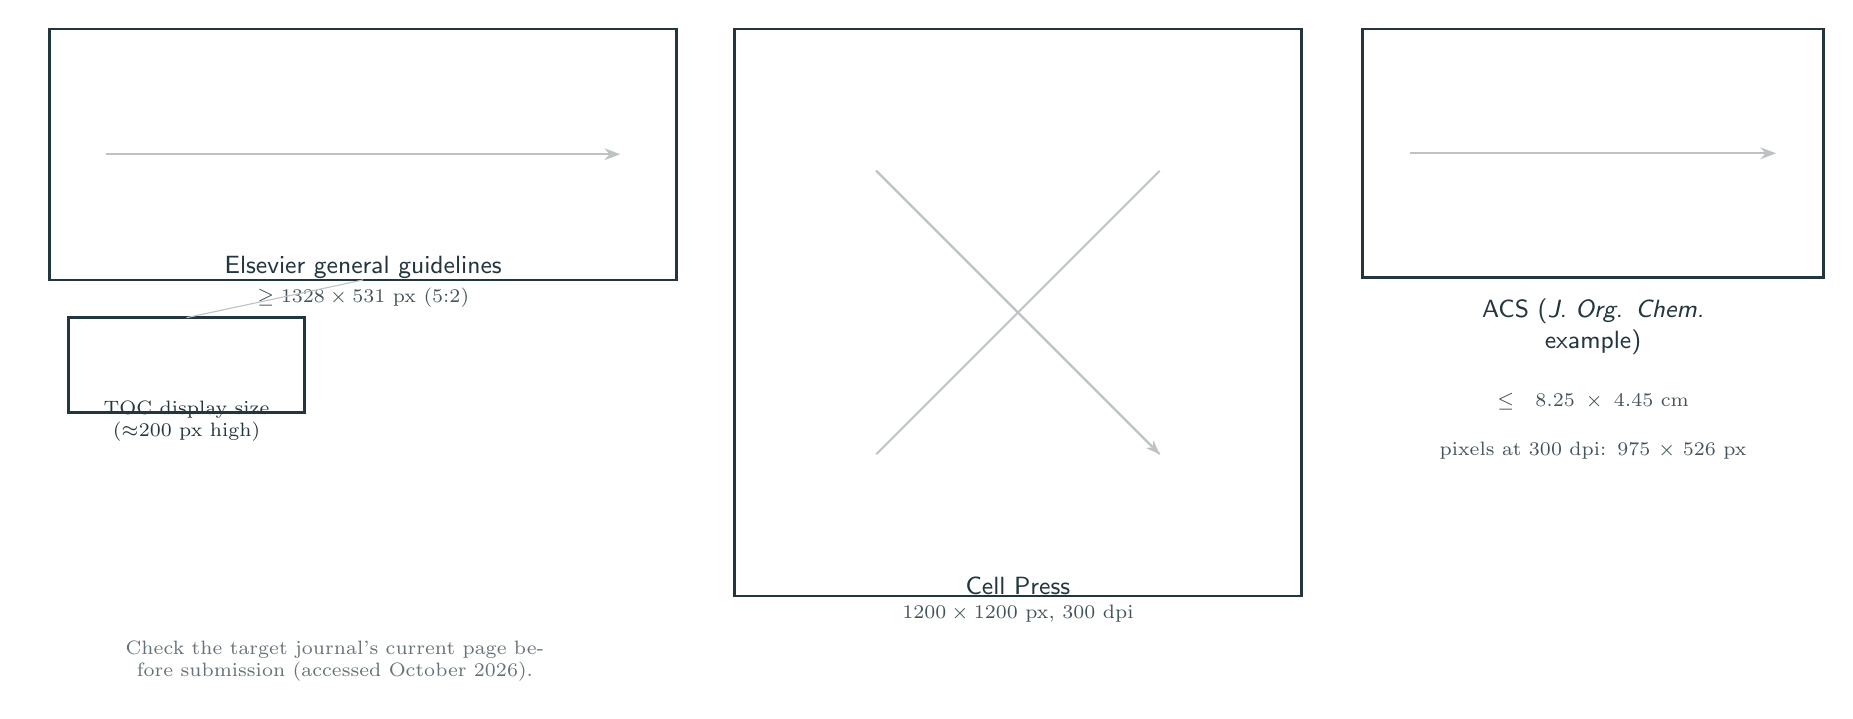
\begin{tikzpicture}[x=0.06mm,y=0.06mm, font=\sffamily\small, text=BookInk]
  \tikzset{
    frame/.style={draw=BookInk, line width=0.35mm, fill=white},
    guide/.style={draw=BookInk!30, line width=0.25mm},
    figcap/.style={font=\sffamily\small, text=BookInk, align=center},
  }
  \def\baseY{1200}
  \draw[frame] (0,\baseY-531) rectangle (1328,\baseY);
  \node[figcap, anchor=south] at (664,\baseY-531-18) {Elsevier general guidelines};
  \node[figcap, font=\scriptsize, text=BookInk!85] at (664,\baseY-531-38)
    {$\geq 1328 \times 531$ px (5:2)};
  \draw[guide, -{Stealth[length=2mm]}] (120, \baseY-265) -- (1208, \baseY-265);
  \draw[frame] (40, \baseY-531-280) rectangle (540, \baseY-531-80);
  \node[figcap, font=\scriptsize, text width=38mm] at (290, \baseY-531-300)
    {TOC display size ($\approx$200 px high)};
  \draw[guide, thin] (664, \baseY-531) -- (290, \baseY-531-80);
  \draw[frame] (1450, 0) rectangle (2650, 1200);
  \node[figcap, anchor=south] at (2050, -18) {Cell Press};
  \node[figcap, font=\scriptsize, text=BookInk!85] at (2050, -38)
    {$1200 \times 1200$ px, 300 dpi};
  \draw[guide] (2050, 600) -- (1750, 900);
  \draw[guide] (2050, 600) -- (2350, 900);
  \draw[guide] (2050, 600) -- (2350, 300);
  \draw[guide] (2050, 600) -- (1750, 300);
  \draw[guide, -{Stealth[length=1.8mm]}] (1750, 900) -- (2350, 300);
  \draw[frame] (2780, \baseY-526) rectangle (3755, \baseY);
  \coordinate (acs-cap) at (3267.5, \baseY-526);
  \node[figcap, anchor=north, text width=50mm, align=center] (acs-t) at ([yshift=-1.5mm]acs-cap)
    {ACS (\textit{J. Org. Chem.}\\example)};
  \node[figcap, font=\scriptsize, text=BookInk!85, anchor=north, text width=50mm, align=center,
    below=2.5mm of acs-t] (acs-m)
    {$\leq 8.25 \times 4.45\ \mathrm{cm}$};
  \node[figcap, font=\scriptsize, text=BookInk!85, anchor=north, text width=50mm, align=center,
    below=1.5mm of acs-m]
    {pixels at 300 dpi: $975 \times 526$ px};
  \draw[guide, -{Stealth[length=2mm]}] (2880, \baseY-263) -- (3655, \baseY-263);
  \node[figcap, font=\scriptsize, text=BookInk!70, anchor=north west, text width=70mm] at (0, -75)
    {Check the target journal's current page before submission (accessed October 2026).};
\end{tikzpicture}
}
\caption{Shapes and scales of three graphical-abstract / TOC requirements, drawn to the same scale. Values from Elsevier's general guidelines, Cell Press, and the ACS \textit{J. Org. Chem.} author guidelines (accessed October 2026). Individual journals may differ; check the target journal's current page before submission. The ACS requirement is physical; pixels are converted at $300\ \text{dpi}$ for comparison only.}\label{fig:ch10-01}
\end{figure}

Figure~\ref{fig:ch10-01} establishes three hard constraints for design:

First, \textbf{aspect ratio locks the direction of the reading path}. Elsevier's $5:2$ canvas is a wide banner suited to a three- or four-stage left-to-right narrative. Cell Press's $1200 \times 1200\ \text{px}$ canvas is a square: lining up small icons across the middle leaves empty bands above and below, so a square calls for a central figure with surrounding nodes or a two-row Z-shaped path. The ACS TOC box is physically small ($8.25\ \text{cm}$ wide), accommodating even fewer visual nodes.

Second, \textbf{the TOC thumbnail height governs minimum font size and element count}. The small box at the lower left of Figure~\ref{fig:ch10-01} shows a constraint highlighted in Elsevier's guide: in the online TOC, the image is scaled down to a window \textbf{about $200\ \text{px}$ high} ($500 \times 200\ \text{px}$ at $5:2$). Even on a $2000 \times 800\ \text{px}$ canvas, linear dimensions shrink to one-quarter in the TOC. Text set at $14\ \text{px}$ height on the original canvas shrinks to $3.5\ \text{px}$ and becomes unreadable.

Third, \textbf{check the target journal's live page before drawing and log the access date}. Sister journals under the same publisher can differ, and rules change over time. Before starting, record the URL, access date, ratio, pixel floor, fonts, and formats in your archive. Our chapter case targets an Elsevier remote-sensing journal using the general guidelines: a \textbf{$5:2$ banner exported at $2000 \times 800\ \text{px}$ ($\ge 1328 \times 531\ \text{px}$) and verified at a $200\ \text{px}$ TOC height}.

\section{From Paper to a Four-Line Contribution Card}

Once canvas dimensions are fixed, the next step is not to write an image prompt immediately, but to distil the paper into a \textbf{four-line contribution card}.

\begin{BookNote}
\textbf{Note:} The research described below is a fictional teaching scenario created for this chapter. Its methods and findings are set conservatively according to domain consensus and do not correspond to the results of any published paper.
\end{BookNote}

Let us review the domain background for our main case. After a wildfire, post-fire assessment requires mapping \textbf{burned area}---the land surface already burned by fire. Because fire removes vegetation and chars the surface, near-infrared (NIR) reflectance drops and shortwave-infrared (SWIR) reflectance rises; the Normalized Burn Ratio $\text{NBR} = (\text{NIR} - \text{SWIR})/(\text{NIR} + \text{SWIR})$ and its pre- to post-fire difference ($\text{dNBR}$) with a fixed threshold provide a standard baseline for burned-area mapping (Chuvieco et al., 2019; Roy et al., 2019). Global moderate-resolution burned-area products such as MODIS MCD64A1 are released monthly at about $500\ \text{m}$ resolution (Giglio et al., 2018), whereas higher-resolution Landsat and Sentinel-2 imagery resolves finer fire perimeters (Roy et al., 2019), and deep-learning semantic segmentation networks have been applied to Sentinel-2 burned-area mapping (Knopp et al., 2020).

Against this background, Zhou's group drafted the following teaching abstract:

\begin{Prompt}
Fictional teaching manuscript for Chapter 10 — not a real study.
Title: Earlier burned-area mapping from Sentinel-2 image pairs with a
segmentation network
Abstract. Burned-area information supports post-fire assessment, but widely
used moderate-resolution products are released monthly. We ask whether burned
area can be mapped as soon as the first cloud-free post-fire Sentinel-2 image
becomes available. We train an encoder-decoder segmentation network on
co-registered pre-fire and post-fire image pairs, using near-infrared and
shortwave-infrared bands, to predict a per-pixel burned probability. On
held-out fire events, the network's maps agree more closely with reference fire
perimeters than a fixed-threshold dNBR baseline, especially along fragmented
edges and in mixed vegetation. Agreement decreases when clouds or smoke obscure
the post-fire scene and in ecoregions that differ from the training data. The
approach maps areas that have already burned; it does not detect active fires
or forecast fire occurrence. Its timeliness is bounded by satellite revisit and
cloud-free acquisitions. We discuss how reference-perimeter uncertainty and
geographic transfer should be evaluated before operational use.
\end{Prompt}

To avoid cramming band lists, co-registration steps, and secondary caveats into the graphical abstract, we use a \textbf{four-line contribution card} (\textbf{Question, Method, Finding, Limits}) governed by three filtering rules:
\begin{enumerate}
\item \textbf{One sentence and one main subject per line:} strip out technical parameters that belong in the Methods section (band numbers, loss functions, training hyperparameters).
\item \textbf{Keep the exact claim strength of the paper in the Finding line:} ``agrees more closely with reference fire perimeters than a fixed-threshold dNBR baseline'' must never be inflated into ``solves burned-area mapping in complex terrain.''
\item \textbf{Choose for the Limits line the boundary conditions whose omission would mislead readers:} here two limits must accompany the finding---first, the method maps \textbf{areas that have already burned, not active fire detection (typically thermal infrared) or fire forecasting}; second, it \textbf{depends on cloud-free views, bounded by satellite revisit (on the order of days) and cloud or smoke cover}.
\end{enumerate}

Table~\ref{tab:ch10-02-card} shows the author-approved contribution card distilled from the abstract.

\begin{table}[htbp]\centering\footnotesize
\setlength{\tabcolsep}{3pt}
\renewcommand{\arraystretch}{1.15}
\caption{Four-line contribution card distilled from the teaching abstract (author-approved version).}\label{tab:ch10-02-card}
\begin{tabularx}{\linewidth}{@{}>{\raggedright\arraybackslash}p{15mm}Y>{\raggedright\arraybackslash}p{34mm}>{\raggedright\arraybackslash}p{34mm}@{}}
\toprule
\textbf{Row} & \textbf{Contribution card content} & \textbf{Source sentence in abstract} & \textbf{What was omitted and why} \\
\midrule
Question & Can burned area be mapped from the first cloud-free post-fire image? & ``We ask whether burned area can be mapped as soon as the first cloud-free post-fire Sentinel-2 image becomes available.'' & Monthly product resolution and post-fire assessment background (left to Introduction) \\
Method & A segmentation network trained on pre-/post-fire Sentinel-2 pairs predicts per-pixel burned probability & ``We train an encoder-decoder segmentation network on co-registered pre-fire and post-fire image pairs...'' & NIR/SWIR band list, co-registration details, and layer count (method details) \\
Finding & On held-out fires, maps match reference perimeters more closely than a fixed-threshold dNBR baseline, especially along fragmented edges & ``On held-out fire events, the network's maps agree more closely with reference fire perimeters than a fixed-threshold dNBR baseline...'' & Specific metric numbers (this teaching scenario uses no numbers and shows boundary agreement visually) \\
Limits & Maps areas already burned---not active-fire detection or forecasting; limited by clouds, smoke, and revisit & ``The approach maps areas that have already burned; it does not detect active fires or forecast fire occurrence. Its timeliness is bounded by...'' & Ecoregion transfer and reference-perimeter error (placed in caption and main text) \\
\bottomrule
\end{tabularx}
\end{table}

Combining all four rows gives a one-sentence contribution summary: \textbf{One cloud-free post-fire image is enough to map burned area more closely to reference perimeters than a fixed threshold---but it maps land that has already burned, and only once the sky clears.}

Next, in \scidraw{}'s Scientific Figure Workflow guide (\sdtool{figure-workflow}), select the ``Graphical Abstract'' route, paste the brief below into the task-brief step, and download a copy (the guide organizes steps without verifying scientific content; full version in the \texttt{cases/} directory of the book repository):

\begin{Prompt}
[Use and audience] Graphical abstract for an Elsevier remote-sensing journal;
readers are remote-sensing and ecology researchers unfamiliar with DL details.
[Dimensions] 5:2 banner, exported at 2000 x 800 px (>= 1328 x 531 px), scaled
to ~200 px high in the online table of contents.
[Goal] Grasp in 5 seconds: first cloud-free post-fire image -> segmentation
network -> burned-area map closer to reference edges than a dNBR threshold;
also see "already-burned area mapping, not fire detection, limited by clouds."
[Materials] Author-verified 4-line contribution card and abstract; no extra claims.
[Objects] (1) Pre-/post-fire flat schematic map tiles (not photos or real data);
(2) encoder-decoder hourglass icon (no layers); (3) output burned-area polygon
tile; (4) comparison inset: reference edge (dark gray solid), model (blue solid),
threshold (light gray dashed); (5) small cloud-covered input tile.
[Relationships] Image pair -> network -> burned-area map (two identical arrows);
comparison inset at right with no arrow; cloud tile near input stage.
[Layout] Left-to-right 4 stages; top 15% for headline, bottom 12% for limits.
[Visual] White background, flat 2D vector style; muted green vegetation, warm
brown-orange burned area, blue-gray network; <= 3 hues plus grays.
[Text] Zero text in base art; overlay in LaTeX/TikZ (<= 35 English words).
[Limits] No flames, smoke plumes, globes, realistic satellites, clocks, alarms,
numbers, or axes; do not use "predict," "real-time," or "global."
\end{Prompt}

Note one key rule in the brief: all ``images'' are drawn as \textbf{flat schematic tiles} and labeled ``schematic, not real satellite data'' in the caption. Photorealistic generated views are easily mistaken for observational evidence; if real satellite imagery is ever needed, use study data or public-domain scenes (such as USGS Landsat) and state the source and processing.

\section{Using SciDraw AI to Turn a PDF into a Candidate Prompt}

When entering \scidraw{}'s graphical-abstract tool (\sdtool{graphical-abstract-maker}), you can upload a paper PDF to generate a visual prompt automatically. Using this entry point safely requires knowing its exact reading boundaries (Figure~\ref{fig:ch10-02}).

\begin{figure}[htbp]\centering
\resizebox{\linewidth}{!}{% FIG ch10-02 paper-to-card (English)
\usetikzlibrary{arrows.meta,calc,fit,positioning}
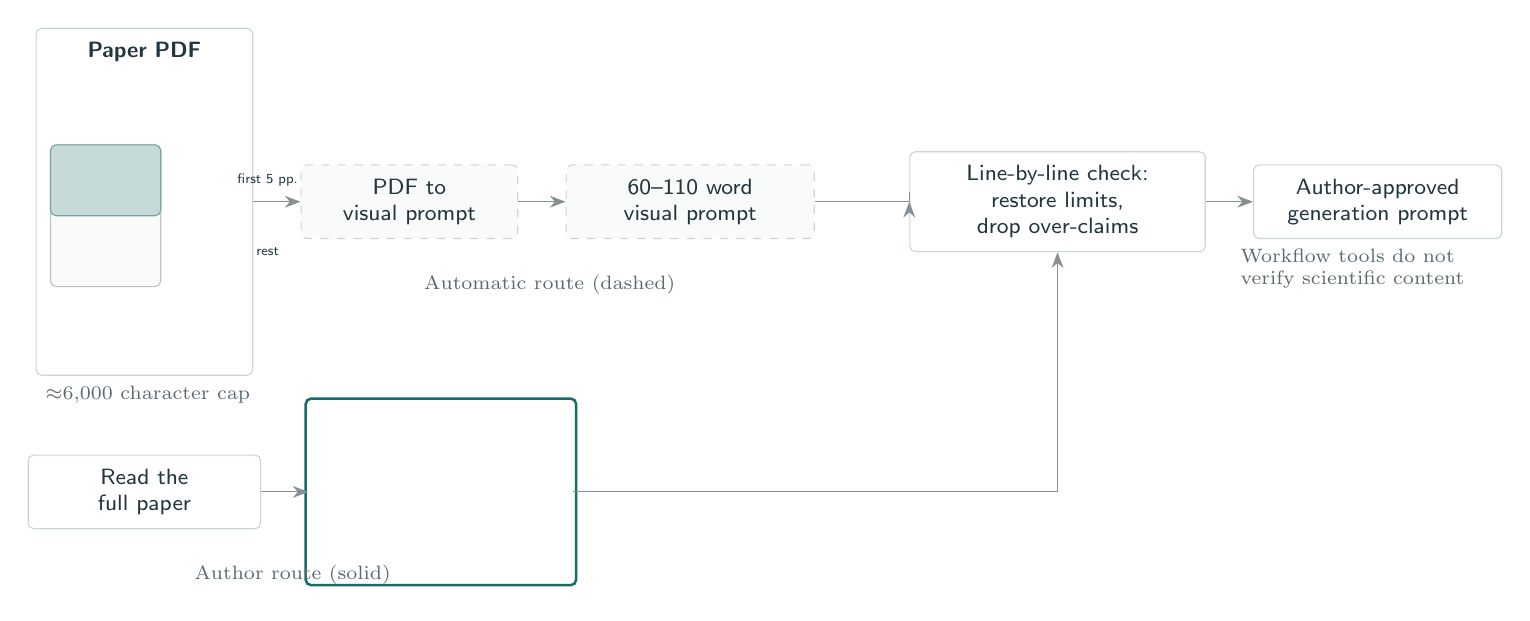
\begin{tikzpicture}[
  font=\sffamily\footnotesize,
  node distance=4mm and 6mm,
  box/.style={
    draw=BookRule, line width=0.4pt, rounded corners=2pt,
    align=center, inner sep=5pt, text=BookInk, text width=24mm,
  },
  autobox/.style={box, dashed, fill=BookPale!40},
  authorbox/.style={box, fill=white},
  limitbox/.style={authorbox, draw=BookTeal, line width=0.9pt},
  flow/.style={-{Stealth[length=2mm]}, draw=BookInk!55, thin},
  note/.style={font=\scriptsize, text=BookInk!75, align=left},
]
  \node[authorbox, minimum width=24mm, minimum height=28mm] (pdf) {%
    \textbf{Paper PDF}\\[2pt]
    \tikz{\draw[fill=BookPale!50, draw=BookInk!30] (0,0) rectangle (1.4,1.8);
      \draw[fill=BookTeal!25, draw=BookTeal!60] (0,0.9) rectangle (1.4,1.8);
      \node[font=\tiny, anchor=west] at (1.55,1.35) {first 5 pp.};
      \node[font=\tiny, anchor=west] at (1.55,0.45) {rest};}};
  \node[autobox, right=of pdf] (auto) {PDF to\\visual prompt};
  \node[autobox, right=of auto, text width=28mm] (prompt) {60--110 word\\visual prompt};
  \node[authorbox, below=10mm of pdf, text width=26mm] (full) {Read the\\full paper};
  \node[authorbox, right=of full, text width=30mm] (card) {%
    Four-line card\\[1pt]
    \begin{tabular}{@{}c@{}}
      Question\\Method\\Finding\\\textbf{Limits}
    \end{tabular}};
  \node[limitbox, fit=(card), inner sep=1pt] {};
  \node[authorbox, right=12mm of prompt, text width=34mm] (merge) {Line-by-line check:\\restore limits,\\drop over-claims};
  \node[authorbox, right=of merge, text width=28mm] (final) {Author-approved\\generation prompt};
  \draw[flow] (pdf) -- (auto);
  \draw[flow] (auto) -- (prompt);
  \draw[flow] (full) -- (card);
  \draw[flow] (prompt.east) -| (merge.west);
  \draw[flow] (card.east) -| (merge.south);
  \draw[flow] (merge) -- (final);
  \node[note, anchor=north west] at (pdf.south west) {$\approx$6{,}000 character cap};
  \node[note, anchor=north] at ($(auto)!0.5!(prompt)+(0,-8mm)$) {Automatic route (dashed)};
  \node[note, anchor=north] at ($(full)!0.5!(card)+(0,-8mm)$) {Author route (solid)};
  \node[note, anchor=north east, text width=32mm] at (final.south east)
    {Workflow tools do not verify scientific content};
\end{tikzpicture}
}
\caption{Two routes from a paper to a graphical-abstract prompt. \scidraw{}'s graphical-abstract tool reads only the first five pages of a PDF (up to about $6{,}000$ characters) and returns a short visual prompt; it does not understand the whole paper. The author's contribution card comes from the full text. Only after a line-by-line comparison---restoring the limits in particular---does the generation prompt take shape.}\label{fig:ch10-02}
\end{figure}

As shown in Figure~\ref{fig:ch10-02}, after uploading a PDF (up to $20\ \text{MB}$), the tool operates under three hard constraints:
\begin{enumerate}
\item \textbf{Reads only the first 5 pages and retains up to about $6{,}000$ characters:} it does not understand the full paper. In a typical manuscript submission, the first five pages reach only the Introduction; failure cases in the Results and limitations in the Discussion are never read unless they also appear in the abstract.
\item \textbf{Compresses text into a $60\text{--}110$-word visual prompt:} internal instructions omit citations, $p$-values, unsupported claims, and minor method details to focus on a visual scene of the core problem, method, and finding.
\item \textbf{Scope limits are often dropped as ``secondary details'':} because compression favors a positive, streamlined visual sequence, negative boundaries such as ``does not detect active fires'' and ``bounded by clouds, smoke, and revisit'' are easily lost, and intensifiers such as ``real-time'' or ``early warning'' can creep in.
\end{enumerate}

Treat the automated prompt as \textbf{``a quick sketch by a second reader who read only the opening pages of your paper.''} Follow a three-step check: first, archive the returned prompt verbatim along with the reading scope; second, audit it line by line against your contribution card (Table~\ref{tab:ch10-03-compare}); third, restore the scope limits and delete any over-claims before generating candidate art.

\begin{table}[htbp]\centering\footnotesize
\setlength{\tabcolsep}{3pt}
\renewcommand{\arraystretch}{1.15}
\caption{Line-by-line audit checklist when using the PDF-to-prompt entry point (what to check against the four-line contribution card and how to revise).}\label{tab:ch10-03-compare}
\begin{tabularx}{\linewidth}{@{}>{\raggedright\arraybackslash}p{15mm}>{\raggedright\arraybackslash}p{31mm}YY@{}}
\toprule
\textbf{Card row} & \textbf{Author card baseline} & \textbf{What to check in the automated 60--110-word prompt} & \textbf{Author revision and restoration action} \\
\midrule
Question & Can burned area be mapped from the first cloud-free post-fire image? & Did it rewrite ``first cloud-free image'' as ``real-time'' or ``early warning,'' or ask for active flames? & Delete ``real-time/early warning'' wording and flames; specify pre- and post-fire static schematic tiles \\
Method & Pre-/post-fire Sentinel-2 pairs fed to a segmentation network & Does it ask for 3D convolution blocks, a glowing brain, or realistic satellites, or add unstudied sensors? & Fix objects to ``two side-by-side square schematic tiles + one clean blue-gray hourglass encoder--decoder icon'' \\
Finding & Closer to reference perimeters than a fixed-threshold dNBR baseline on test fires & Does it draw only the output map while omitting the baseline comparison, or ask for bar charts and percentages? & Add Stage (4): ``three boundary lines on the same patch (dark-gray solid reference, blue solid model, light-gray dashed threshold),'' with no numbers \\
Limits & Already-burned area mapping (not fire detection/forecasting); bounded by clouds, smoke, and revisit & Check whether any visual element expresses ``needs cloud-free views'' and whether blank bands are reserved for limit text & Restore a ``small tile partly covered by a gray cloud'' at the input stage, and reserve top $15\%$ and bottom $12\%$ empty bands \\
\bottomrule
\end{tabularx}
\end{table}

After auditing line by line and restoring the scope limits, we obtain the author-approved generation prompt for the graphical-abstract or drawing workspace:

\begin{Prompt}
Graphical abstract, wide 5:2 banner, white background, flat 2D vector style,
no gradients, no shadows, no 3D effects.
Include NO text, letters, or numbers anywhere; labels will be added later.
Four stages from left to right:
(1) Two side-by-side square schematic map tiles (pre-fire: muted green
    vegetation patches; post-fire: the same patch with a warm brown-orange
    burned area in the middle), plus a smaller square tile partly covered by a
    flat gray cloud in the corner of the input area;
(2) A blue-gray hourglass network icon (encoder-decoder), no neuron layers;
(3) Output map of the same patch: crisp warm brown-orange burned polygon;
(4) Small comparison inset on the same patch outline: dark-gray solid reference
    perimeter, blue solid line closely following it, light-gray dashed line
    clearly deviating from it.
Two identical dark-gray flow arrows connect (1)->(2) and (2)->(3); no arrow
between (3) and (4). Leave top 15% and bottom 12% empty. Palette only: muted
green, warm brown-orange, blue-gray, blue, and grays. No flames, smoke, globes,
realistic satellites, clocks, alarms, charts, or axes.
\end{Prompt}

\section{Two Composition Candidates: Narrative versus Central Figure}

Clicking ``generate 4 candidates'' from one prompt does not compare compositions: \textbf{batch outputs sharing a single prompt are merely random variations of the same layout}. Genuine composition selection requires specifying distinct spatial structures in separate prompts. Here we compare the two primary graphical-abstract layouts: \textbf{left-to-right narrative (Candidate A)} and \textbf{central figure (Candidate B)}.

\textbf{Candidate A (left-to-right narrative)} lays out ``Input $\rightarrow$ Model $\rightarrow$ Output $\rightarrow$ Finding'' across four horizontal stages. Key parts of the submitted English prompt are shown below (full version in the \texttt{cases/} directory of the book repository):

\begin{Prompt}
Graphical abstract base art, wide banner, aspect ratio 5:2 (2000 x 800 px),
pure white background, flat 2D vector illustration, flat fills, thin dark gray
outlines, no gradients, no shadows, no 3D, no photographic texture.
ABSOLUTELY NO TEXT: no letters, no words, no numbers, no symbols, no labels.
Keep the top 15% and the bottom 12% of the image completely empty.
Four equal-width stages from left to right, vertically centered:
1. Input (x 0.04-0.25): two square map tiles side by side (left: muted green
   vegetation with a thin pale-blue river line; right: same patch and river with
   an irregular warm brown-orange burned area). Above them, smaller, a third
   square tile partly covered by a flat light-gray cloud shape.
2. Model (x 0.30-0.46): a single blue-gray hourglass shape of stacked rounded
   rectangles that narrow to a waist and widen again (encoder-decoder).
3. Output (x 0.52-0.72): one square map tile of the same patch in very pale gray
   with a crisp warm brown-orange burned-area polygon.
4. Comparison (x 0.77-0.96): a small square inset showing three boundary lines:
   dark gray solid (reference), blue solid closely following it, light gray
   dashed clearly deviating from it.
Two identical dark gray arrows connect stage 1 to 2 and 2 to 3; no arrow between
3 and 4. Do not draw: flames, smoke, globes, satellites, clocks, alarms, charts.
\end{Prompt}

We ran this prompt twice, selected the first run as the Candidate A base image, and overlaid stage numbers in LaTeX for critique (Figure~\ref{fig:ch10-03}).

\begin{figure}[htbp]\centering
\begin{tikzpicture}
\node[anchor=south west,inner sep=0] (img) at (0,0) {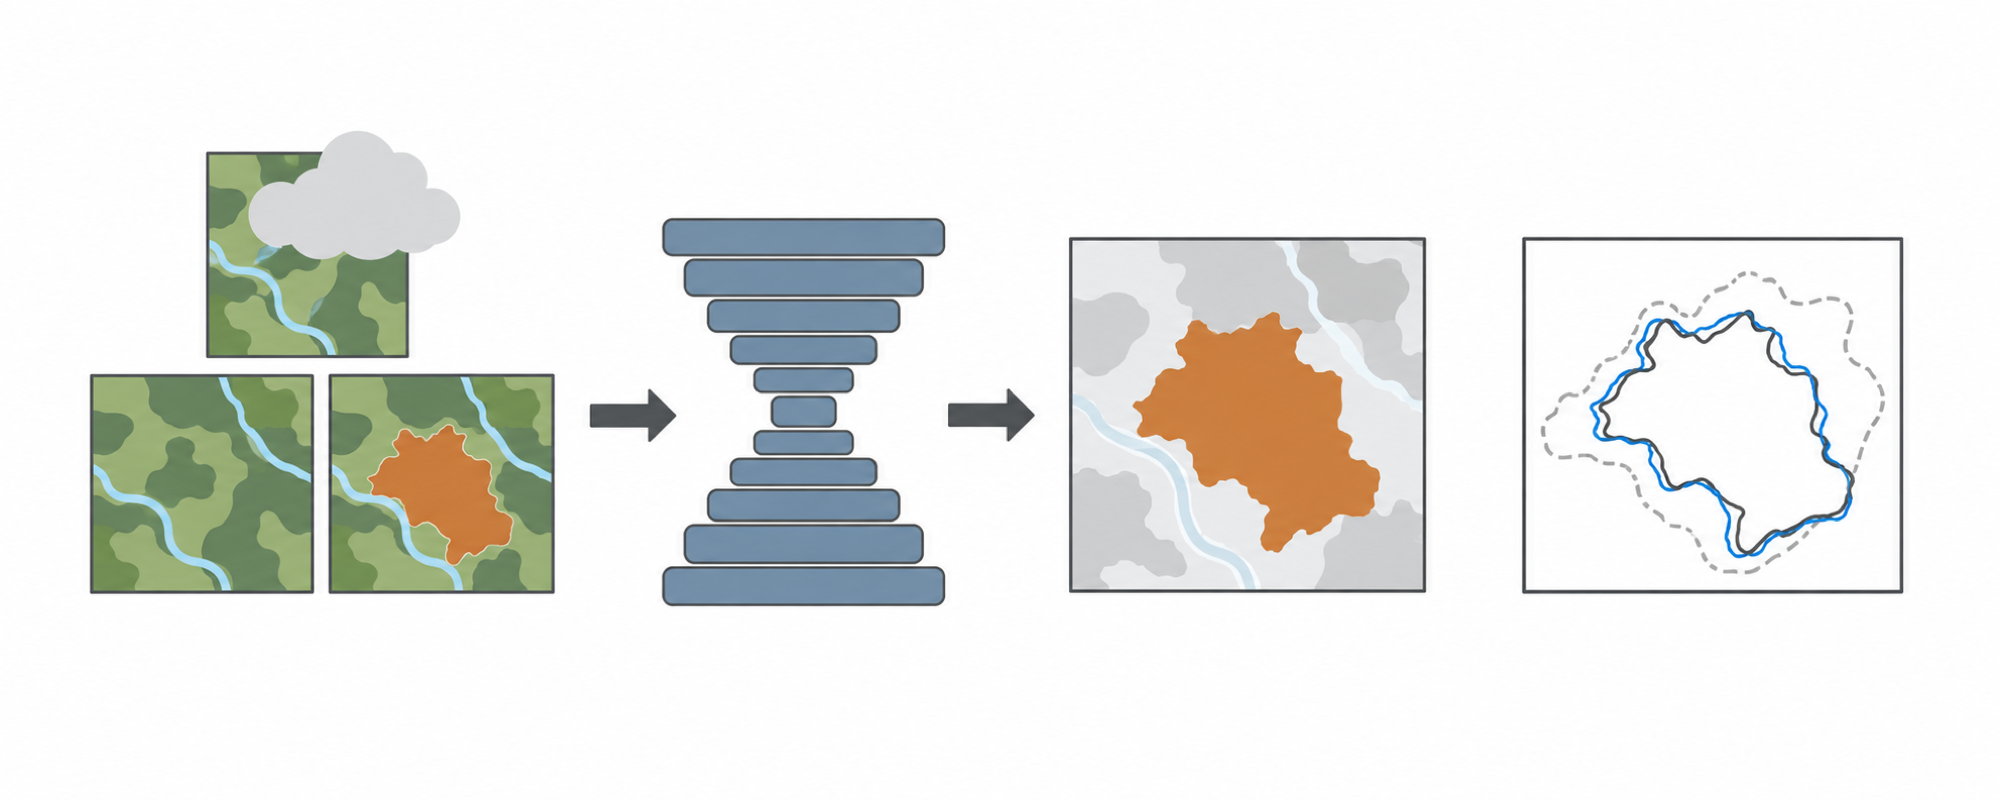
\includegraphics[width=\linewidth]{figures/ch10/ch10-03-composition-a-narrative.png}};
\begin{scope}[x={(img.south east)},y={(img.north west)}]
  \tikzset{stglbl/.style={font=\sffamily\scriptsize\bfseries,text=BookInk,fill=white,fill opacity=0.90,text opacity=1,inner sep=1.5pt,align=center}}
  \node[stglbl] at (0.165,0.16) {(1) Input pair \& cloud limit};
  \node[stglbl] at (0.40,0.16) {(2) Segmentation network};
  \node[stglbl] at (0.62,0.16) {(3) Burned-area map};
  \node[stglbl] at (0.855,0.16) {(4) Edge comparison};
\end{scope}
\end{tikzpicture}
\caption{Composition A: left-to-right narrative. Input, model, output, and finding occupy four stages from left to right; reading starts in one place and ends on the comparison. The cloud tile puts ``needs cloud-free views'' where every reader passes. Base art generated by an image model; all image tiles are schematic.}\label{fig:ch10-03}
\end{figure}

Inspecting the actual artwork in Figure~\ref{fig:ch10-03}: all four stages are present; the pre- and post-fire tiles on the left share matching river bends with the cloud-obscured tile above them; the middle shows a single-column hourglass of 10 rounded rectangles; Stages (1)$\rightarrow$(2) and (2)$\rightarrow$(3) are linked by two identical dark-gray filled arrows with no arrow between (3) and (4); and the comparison box on the right separates the dark-gray solid line, the closely tracking blue solid line, and the deviating light-gray dashed line. Three minor deviations also appear: the cloud is drawn fairly large and extends slightly above its small tile frame; the four stages are not strictly equal in width (the input pair reaches about $x=0.28$, and the output tile is larger than one input tile); and fills show slight tonal variation rather than pure flat color. Run 2 shrank the cloud neatly, but dropped the dark-gray outlines around the hourglass and lost geometric consistency across tiles, so Run 1 was selected.

Now examine \textbf{Candidate B (central figure)}: Stage (3)'s burned-area map is enlarged at the center, while the pre-fire tile, post-fire tile (with its cloud-limit tile), segmentation network, and boundary comparison inset sit at the four corners, connected to the center by plain gray lines without arrowheads. Key parts of the English prompt are shown below (full version in the \texttt{cases/} directory of the book repository):

\begin{Prompt}
Graphical abstract base art, wide banner, aspect ratio 5:2 (2000 x 800 px),
pure white background, flat 2D vector illustration, thin dark gray outlines.
ABSOLUTELY NO TEXT: no letters, words, numbers, symbols, labels or title.
Central composition. In the exact center, one large square top-down schematic
map tile (about 70% of image height) of a landscape patch in very pale gray with
a crisp warm brown-orange burned-area polygon and a thin pale-blue river line.
Around it, four small elements, each about one quarter the size of the center:
- upper left: small tile of the same patch in muted green vegetation (before);
- lower left: small tile of the same patch with a warm brown-orange area (after),
  and next to it an even smaller tile partly covered by a flat light gray cloud;
- upper right: small blue-gray hourglass shape of stacked rounded rectangles;
- lower right: small square inset with three boundary lines: dark gray solid,
  blue solid closely following it, light gray dashed clearly deviating.
Thin plain gray connector lines without arrowheads run from each small element
toward the central tile. Do not draw: flames, smoke, globes, satellites, clocks.
\end{Prompt}

The central composition took three runs, and the two rejected runs expose common pitfalls of multi-element radial layouts: in Run 1, the central map retained green vegetation instead of a pale-gray background and the network split into two columns; Run 2 fixed the pale-gray center and single-column hourglass, but attached the lower-left connector line directly to the tiny cloud-covered tile, leaving the main post-fire input tile disconnected; only in Run 3---after specifying exact connector attachment points and detaching the cloud tile---did we obtain a structurally sound Candidate B (Figure~\ref{fig:ch10-04}).

\begin{figure}[htbp]\centering
\begin{tikzpicture}
\node[anchor=south west,inner sep=0] (img) at (0,0) {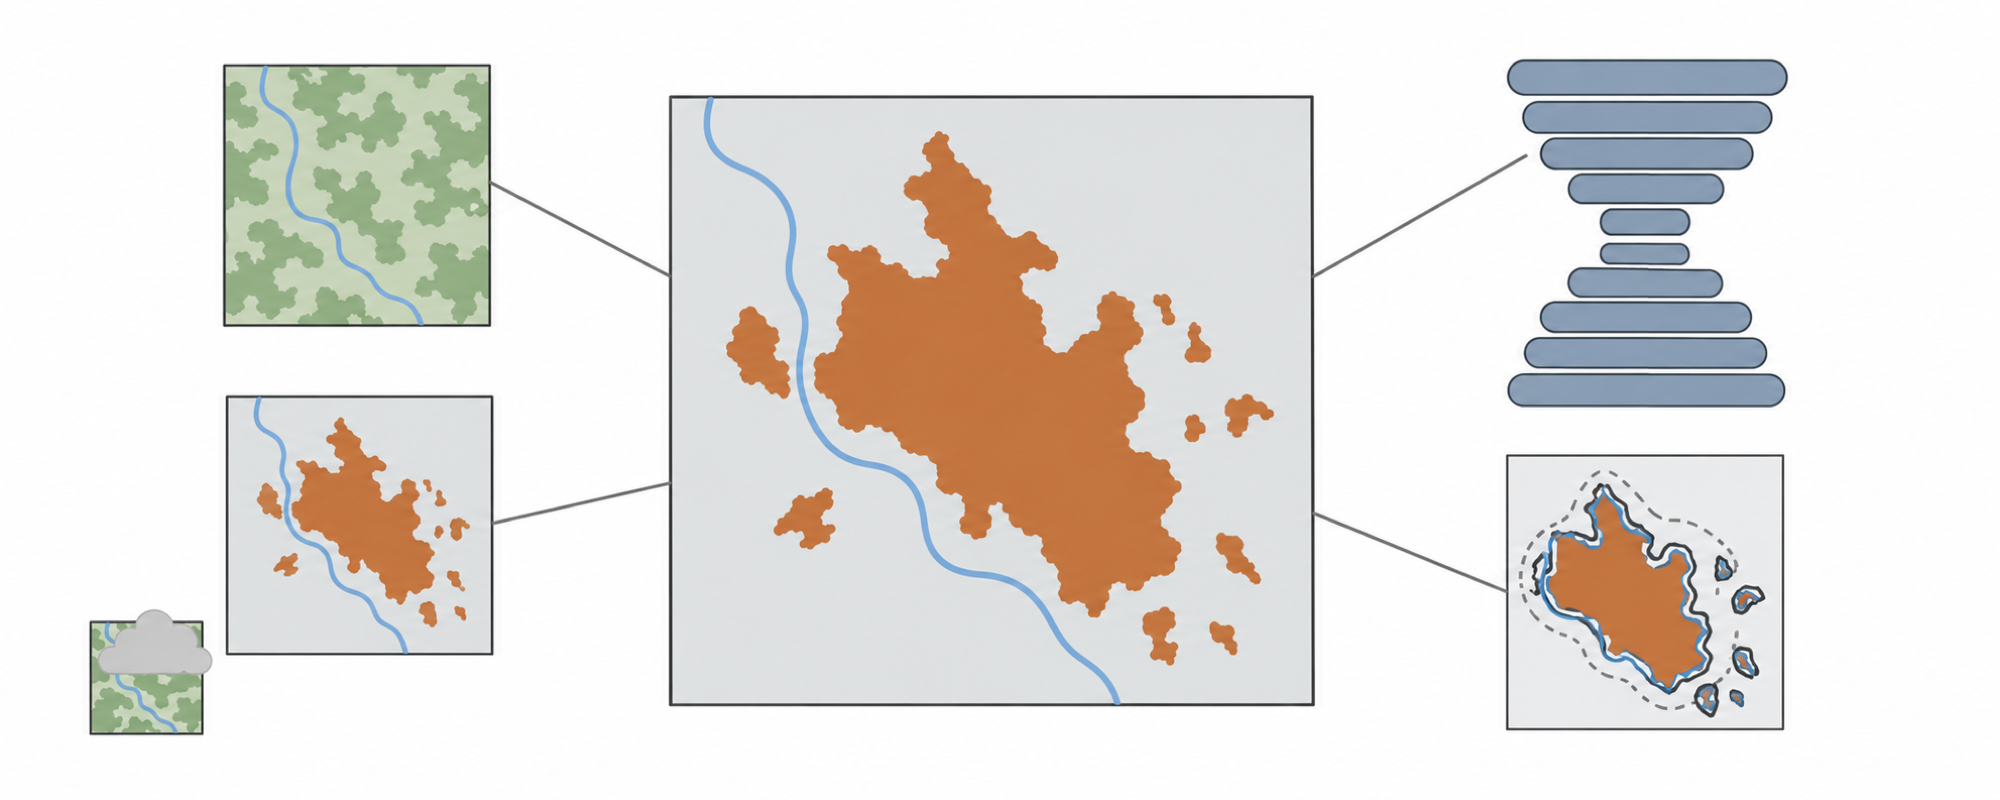
\includegraphics[width=\linewidth]{figures/ch10/ch10-04-composition-b-central.png}};
\begin{scope}[x={(img.south east)},y={(img.north west)}]
  \tikzset{stglbl/.style={font=\sffamily\scriptsize\bfseries,text=BookInk,fill=white,fill opacity=0.90,text opacity=1,inner sep=1.2pt,align=center}}
  \node[stglbl] at (0.175,0.54) {(1) Pre-fire tile};
  \node[stglbl] at (0.175,0.11) {(1) Post-fire \& cloud tiles};
  \node[stglbl] at (0.82,0.45) {(2) Segmentation network};
  \node[stglbl] at (0.49,0.05) {(3) Burned-area map (center)};
  \node[stglbl] at (0.82,0.04) {(4) Edge comparison};
\end{scope}
\end{tikzpicture}
\caption{Composition B: central figure. Same content as Figure~\ref{fig:ch10-03}. The central map draws the eye, but in a $5:2$ banner the surrounding elements shrink, and the comparison with the threshold method retreats to the lower-right corner---the first thing lost at thumbnail size. For a $1200\ \text{px}$ square format this layout adapts more easily.}\label{fig:ch10-04}
\end{figure}

Figure~\ref{fig:ch10-04} also shows the limits of a central layout in a $5:2$ banner: the central map takes up about $77\%$ of canvas height, pushing surrounding elements to the sides; the upper-right hourglass is oversized, whereas the lower-right comparison inset carrying the finding is squeezed into a corner where its small patches and three contour lines blur together when scaled down; and the cloud-limit tile retreats to the far lower-left corner. Table~\ref{tab:ch10-04-ab} compares the two compositions systematically.

\begin{table}[htbp]\centering\footnotesize
\setlength{\tabcolsep}{3pt}
\renewcommand{\arraystretch}{1.15}
\caption{Comparison between Candidate A (left-to-right narrative) and Candidate B (central figure).}\label{tab:ch10-04-ab}
\begin{tabularx}{\linewidth}{@{}>{\raggedright\arraybackslash}p{25mm}YY@{}}
\toprule
\textbf{Criterion} & \textbf{Candidate A: Left-to-right narrative (Figure~\ref{fig:ch10-03})} & \textbf{Candidate B: Central figure (Figure~\ref{fig:ch10-04})} \\
\midrule
Reading entry point & Unique (pre-/post-fire pair at far left) & Eye lands on the center map first; inputs and comparison scatter around four corners \\
Endpoint on ``Finding''? & Yes (boundary comparison inset at far right) & Center map is the output; the ``closer than threshold'' comparison is pushed to the lower-right corner \\
$5:2$ banner fit & Good; four horizontal stages leave top and bottom text bands & Center map occupies $\approx 77\%$ of height, leaving little room for full-width text bands \\
$200\ \text{px}$ high thumbnail & Stage icons and main contours remain distinguishable & Surrounding small elements and fine lower-right comparison lines blur first \\
Scope-limit placement & Cloud icon above input pair + bottom full-width text line, right on the reading path & Cloud icon pushed to the far lower-left corner, easy to overlook \\
If adapted to $1200\ \text{px}$ square & Must fold into two rows (Z-shaped reading path) & Four-corner hub-and-spoke topology fits a square naturally \\
\midrule
\textbf{Conclusion} & \textbf{Select A} (target is an Elsevier $5:2$ banner) & Keep as a backup for square-format venues \\
\bottomrule
\end{tabularx}
\end{table}

Both candidates look clean, but the choice rests on aspect ratio, reading entry and exit points, and limit visibility at thumbnail scale---not subjective aesthetics. If the paper were later reformatted for a $1200 \times 1200\ \text{px}$ square format, Candidate B would adapt more naturally.

\section{Over-Claiming: When the Image Says More Than the Paper}

Suppose a co-author looks at Candidate A, says ``It looks too plain---make it dramatic and highlight AI's early-warning capability and global significance,'' and submits the following counter-example prompt:

\begin{Prompt}
Deliberately over-dramatic graphical abstract base art for a teaching
counter-example, wide banner, aspect ratio 5:2 (2000 x 800 px).
Dark blue gradient background with glowing accents.
Left: a photorealistic satellite-style top-down view of a forest with a bright
red-orange active fire front and thick gray smoke plumes.
Center: a glowing glossy 3D "AI brain" made of circuit lines, with light rays.
Right: a 3D Earth globe covered by a bright grid, with several red flame icons
on it, a red triangular alarm icon, and an alarm clock.
Glossy, cinematic, high contrast, lens flare.
NO TEXT: no letters, no words, no numbers, no symbols, no labels.
Leave a dark empty band across the top 18% for a headline.
\end{Prompt}

Generating this counter-example base image revealed an important detail: even though the prompt specified \texttt{NO TEXT}, Run 1 drew numerals $1\text{--}12$ on the clock dial and an exclamation mark inside the red triangle, and Run 2 still left a short vertical tick mark at the 12 o'clock position resembling the digit ``1.'' Only Run 3---after we required a blank dial with only two hands and an empty warning triangle---eliminated all built-in characters. On top of the Run 3 base image, we overlaid typical exaggerated headlines, a percentage badge, and a prediction slogan in TikZ (along with a ``fictional exaggerated counter-example'' watermark to prevent misuse if screenshotted), marking seven over-claims as \textbf{O1--O7} (Figure~\ref{fig:ch10-05}).

\begin{figure}[htbp]\centering
\begin{tikzpicture}
\node[anchor=south west,inner sep=0] (img) at (0,0) {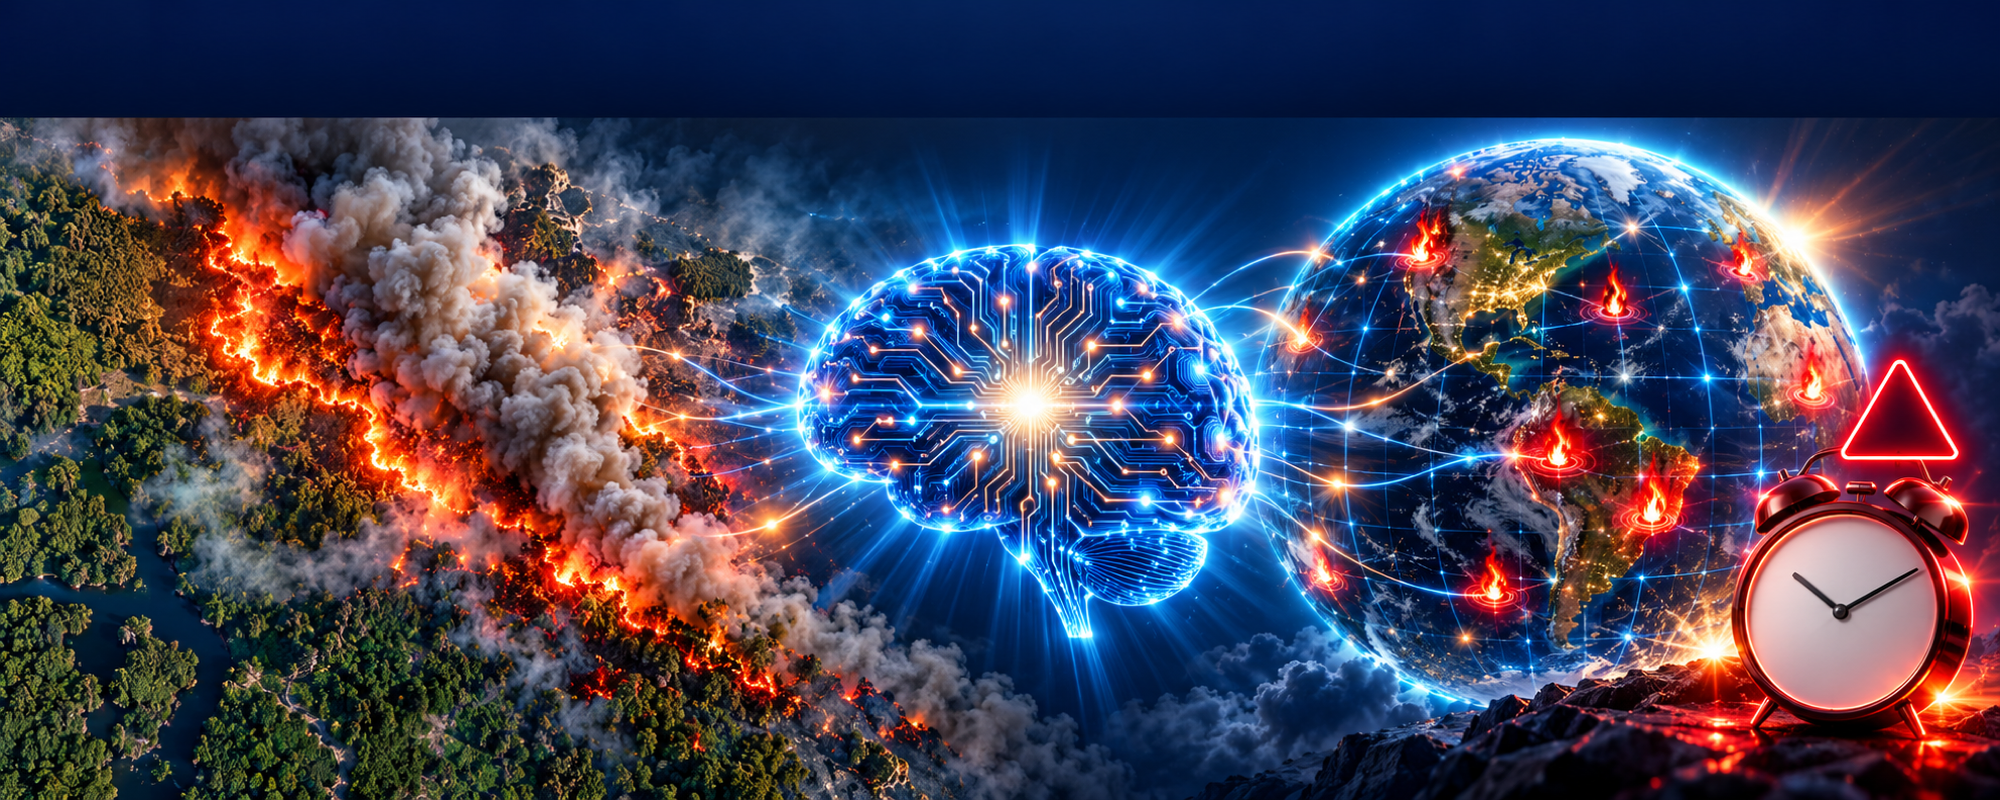
\includegraphics[width=\linewidth]{figures/ch10/ch10-05-overclaim.png}};
\begin{scope}[x={(img.south east)},y={(img.north west)}]
  \tikzset{
    overtxt/.style={font=\sffamily\bfseries,text=white,align=center},
    badmark/.style={draw=red!85!black,very thick,rounded corners=2pt,fill=white,fill opacity=0.92,text opacity=1,text=red!85!black,font=\sffamily\bfseries\scriptsize,inner sep=1.5pt}
  }
  \node[overtxt,font=\sffamily\normalsize\bfseries] at (0.52,0.92) {Real-time global wildfire AI};
  \node[font=\sffamily\scriptsize\bfseries,text=yellow!90!white,fill=black!65,inner sep=1.5pt,rounded corners=1pt] at (0.50,0.81) {[Fictional exaggerated counter-example $\cdot$ not a real study]};
  \node[overtxt,font=\sffamily\large\bfseries,text=yellow!95!white,fill=black!55,inner sep=2pt,rounded corners=2pt] at (0.50,0.45) {99\% accuracy};
  \node[overtxt,font=\sffamily\footnotesize\bfseries,fill=red!75!black,inner sep=2pt,rounded corners=2pt] at (0.72,0.12) {Predicts fires before they start};
  \node[badmark] at (0.09,0.34) {O1};
  \node[badmark] at (0.19,0.50) {O2};
  \node[badmark] at (0.77,0.56) {O3};
  \node[badmark] at (0.91,0.24) {O4};
  \node[badmark] at (0.37,0.45) {O5};
  \node[badmark] at (0.24,0.92) {O6};
  \node[badmark] at (0.27,0.70) {O7};
\end{scope}
\end{tikzpicture}
\caption{Counter-example: an over-claiming graphical abstract (fictional). A photographic ``satellite image,'' a fire front, a globe, an alarm clock, and an unqualified percentage inflate burned-area mapping into observational evidence, active-fire detection, global coverage, forecasting, and universal accuracy. The headline and number are deliberately exaggerated fiction, not results. Base art generated by an image model.}\label{fig:ch10-05}
\end{figure}

Table~\ref{tab:ch10-05-overclaim} breaks down the seven over-claims (O1--O7) in Figure~\ref{fig:ch10-05} and their conservative fixes.

\begin{table}[htbp]\centering\footnotesize
\setlength{\tabcolsep}{3pt}
\renewcommand{\arraystretch}{1.12}
\caption{Breakdown and conservative correction of the seven over-claims (O1--O7) in Figure~\ref{fig:ch10-05}.}\label{tab:ch10-05-overclaim}
\begin{tabularx}{\linewidth}{@{}c>{\raggedright\arraybackslash}p{25mm}>{\raggedright\arraybackslash}p{25mm}>{\raggedright\arraybackslash}p{26mm}Y@{}}
\toprule
\textbf{\#} & \textbf{Over-claiming element} & \textbf{What it implies} & \textbf{What the paper supports} & \textbf{Conservative correction} \\
\midrule
O1 & Photorealistic overhead forest ``image'' & Real satellite observational photo & Schematic pre-/post-fire pair; target is burned ground & Revert to flat schematic tiles; note ``schematic, not real satellite data'' in caption \\
O2 & Bright fire front, flame icons, and red warning triangle & Active fire detection and emergency alerting & Post-fire burned-area mapping & Delete fire front, flames, and alarm; draw burned area as a static warm brown-orange polygon \\
O3 & Globe with glowing global grid & Applicable globally across ecoregions & Tested on held-out fires; cross-ecoregion transfer unverified & Delete globe and grid; draw a single schematic patch and state test scope \\
O4 & Alarm clock and ``Predicts fires before they start'' & Forecasts fire ignition before it starts & Maps burned area once first cloud-free post-fire image arrives & Delete clock and ``predicts''; write ``from the first clear post-fire image'' \\
O5 & Large ``99\% accuracy'' badge & Universal high accuracy number & Reports closer agreement with reference edges than fixed-threshold dNBR; numbers need metric and baseline context & Delete numbers; express the comparative finding via the three-line boundary inset \\
O6 & ``Real-time global wildfire AI'' headline & Global coverage, real-time response & Bounded by satellite revisit and clouds/smoke & Change headline to ``Burned-area maps from the first clear post-fire image'' \\
O7 & Dense smoke pierced by AI light beams, with cloud limit omitted & Unaffected by clouds or smoke; all-weather penetration & Optical agreement drops under clouds or smoke; requires cloud-free views & Remove smoke-piercing beams; restore gray cloud tile at input and bottom limits line \\
\bottomrule
\end{tabularx}
\end{table}

Notice \textbf{O7} in particular: thick 3D smoke billows over the forest on the left while glowing beams from the central brain pierce straight through the smoke toward the global grid, and the ``needs cloud-free views'' cloud tile has vanished---falsely implying that optical bands penetrate thick wildfire smoke.

\begin{BookNote}
\textbf{Principle: Every icon in a graphical abstract is a declarative sentence.} Reviewers and readers read ``flames'' as ``detects active fire,'' a ``globe'' as ``works globally,'' an ``alarm clock'' as ``early warning,'' and ``beams piercing smoke'' as ``immune to cloud and smoke cover.'' During inspection, translate every visual element into a sentence and find its evidence in the paper; if you cannot find it, delete the element.
\end{BookNote}

When faced with a thoroughly derailed draft like Figure~\ref{fig:ch10-05}, do not use it as a reference image for piecemeal patching; instead, \textbf{return directly to the Candidate A base image (Figure~\ref{fig:ch10-03})} and issue a focused revision instruction:

\begin{Prompt}
Start from Draft A; do not use the dramatic version. Keep Draft A's four-stage
layout and all existing objects unchanged.
No flames, smoke plumes, red alarms, globes, alarm clocks, or photorealistic
imagery, and no numbers or text.
Make only two changes: (1) enlarge the output burned-area map tile to about 1.2
times the input tile size; (2) thicken the three boundary lines in the
comparison inset so the deviation between the light-gray dashed line and the
blue solid line stays visible when scaled down.
\end{Prompt}

\section{Final Artwork, the Thumbnail Test, and Verification}

We turn the revision instructions above into the final English base prompt (full version in the \texttt{cases/} directory of the book repository):

\begin{Prompt}
Final graphical abstract base art, wide banner, aspect ratio 5:2,
2000 x 800 px, pure white background, flat 2D vector illustration, flat fills,
uniform thin dark gray (#3A3A3A) outlines, no gradients, no shadows, no 3D.
THIS IMAGE MUST CONTAIN NO TEXT AT ALL: no letters, words, numbers, symbols.
EMPTY BANDS: keep y 0.00-0.15 (top), y 0.76-0.84 (caption strip under the four
stages) and y 0.88-1.00 (bottom) completely white.
Four stages, all objects vertically within y 0.18-0.72:
1. x 0.04-0.25: two square schematic map tiles side by side (left: muted green
   #A8C3A0 vegetation; right: same patch with #C8743C burned area), same river.
   Smaller tile partly covered by a flat light gray (#D5D5D5) cloud at upper left.
2. x 0.30-0.45: one blue-gray (#8FA3B8) hourglass of stacked rounded rectangles.
3. x 0.50-0.73: one larger square map tile in very pale gray with a crisp
   #C8743C burned-area polygon (about 1.2 times the input tiles).
4. x 0.77-0.96: a square inset with three thick boundary lines: #3A3A3A solid
   (reference), #2F6DB5 solid closely following it, #A0A0A0 dashed deviating.
Two identical #3A3A3A arrows: stage 1 -> 2, stage 2 -> 3; no arrow between 3 and 4.
\end{Prompt}

The final base artwork also took three runs: without a reference image, Run 1 split the hourglass into left and right columns forming an X-shape with weak dashed-line separation, and Run 2 fixed the network and thickened the lines but generated a different river course and burned polygon from Candidate A. In Run 3, \textbf{attaching Candidate A (Figure~\ref{fig:ch10-03}) as a visual reference} preserved Candidate A's river course, burned-area outline, single-column hourglass, and twin flow arrows while thickening the three comparison contours in Stage (4). Three minor residual deviations remain: the output square side length is about $1.6$ times a single input tile (aligning with the combined height of the stacked left tiles rather than strictly $1.2$ times), some frame bottoms reach about $y=0.75$, and empty-band RGB values fluctuate between $249$ and $255$. None of these details affects the scientific message, and all three text bands are clean.

We then overlay seven vector text elements (Table~\ref{tab:ch10-06-text}) in TikZ on the text-free base to produce the final graphical abstract (Figure~\ref{fig:ch10-06}).

\begin{table}[htbp]\centering\footnotesize
\setlength{\tabcolsep}{3pt}
\renewcommand{\arraystretch}{1.15}
\caption{Vector text layers (T1--T7) overlaid on the final graphical abstract (Figure~\ref{fig:ch10-06}).}\label{tab:ch10-06-text}
\begin{tabularx}{\linewidth}{@{}cY>{\raggedright\arraybackslash}p{30mm}>{\raggedright\arraybackslash}p{32mm}@{}}
\toprule
\textbf{\#} & \textbf{English vector text layer} & \textbf{Contribution-card role} & \textbf{Position and size tier} \\
\midrule
T1 & Burned-area maps from the first clear post-fire image & Question \& takeaway & $(0.50,0.92)$ top center; largest tier \\
T2 & Pre-/post-fire Sentinel-2 pair & Method (input) & Below Stage (1); medium (TOC-legible) \\
T3 & Segmentation network & Method (model) & Below Stage (2); medium (TOC-legible) \\
T4 & Burned-area map & Method (output) & Below Stage (3); medium (TOC-legible) \\
T5 & Closer to reference edges than dNBR threshold & Finding (comparison) & Below Stage (4); medium (TOC-legible) \\
T6 & Maps areas already burned $\cdot$ not fire detection or forecasting $\cdot$ needs cloud-free views & Limits (mandatory scope) & $(0.50,0.04)$ bottom center; small (article-page legible) \\
T7 & reference / model / threshold & Comparison legend & Below T5 in Stage (4); smallest tier \\
\bottomrule
\end{tabularx}
\end{table}

\begin{figure}[htbp]\centering
\begin{tikzpicture}
\node[anchor=south west,inner sep=0] (img) at (0,0) {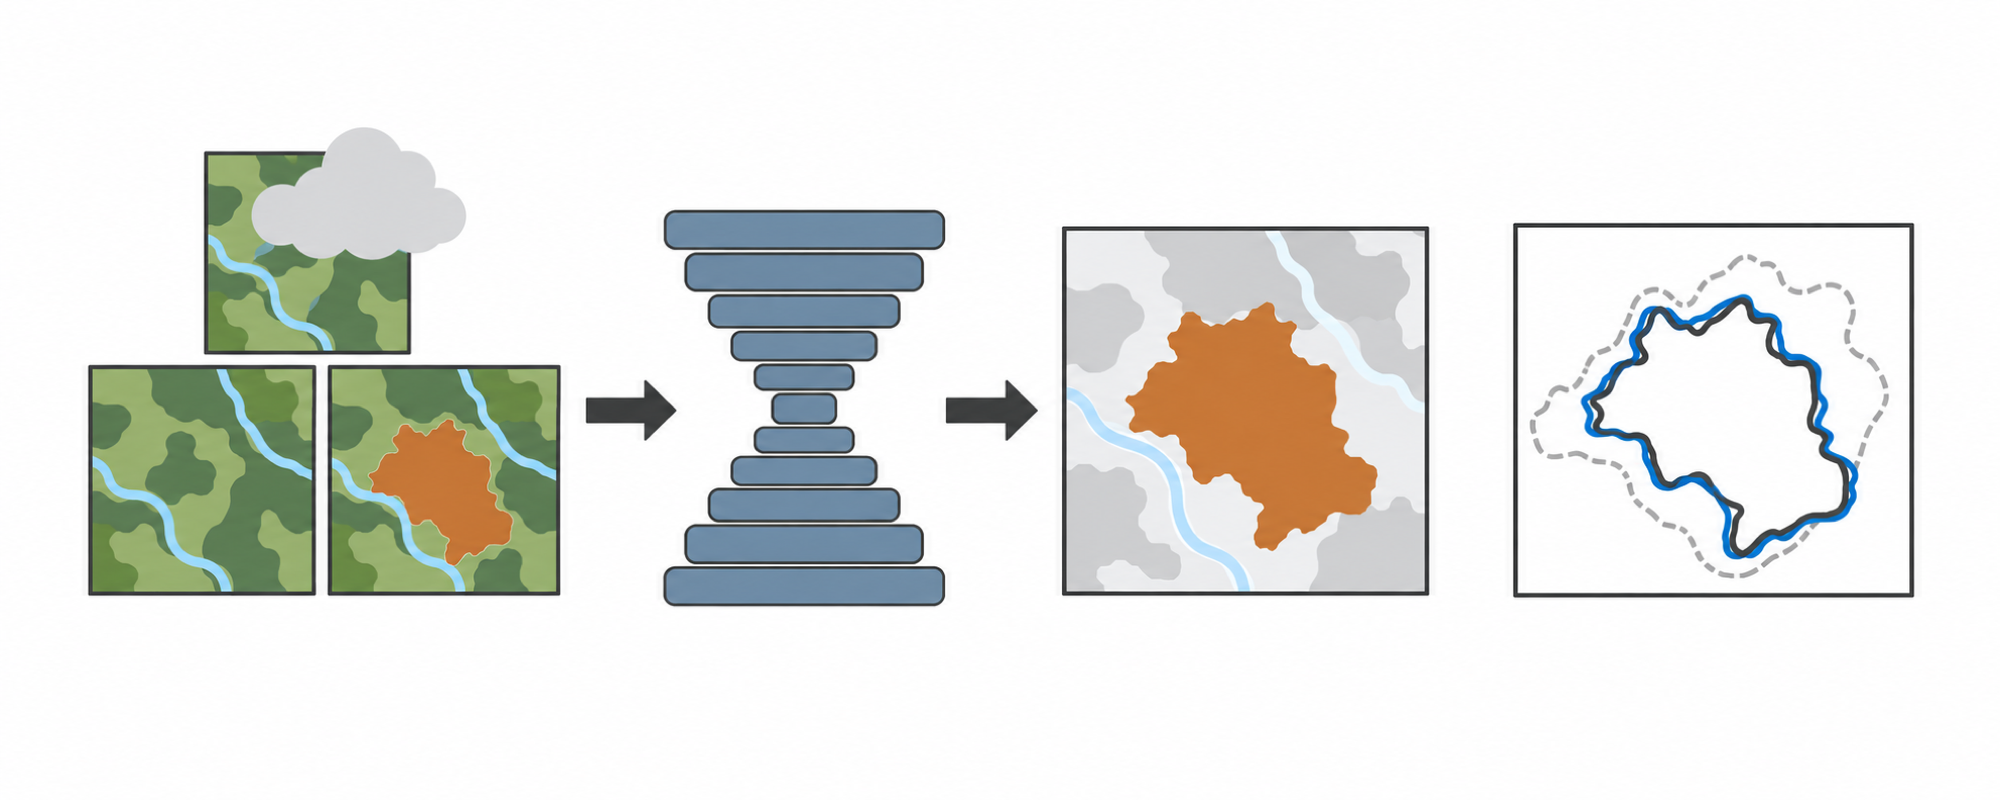
\includegraphics[width=\linewidth]{figures/ch10/ch10-06-final-base.png}};
\begin{scope}[x={(img.south east)},y={(img.north west)}]
  \tikzset{
    t1style/.style={font=\sffamily\small\bfseries,text=BookInk,align=center},
    tstg/.style={font=\sffamily\scriptsize\bfseries,text=BookInk,fill=white,fill opacity=0.90,text opacity=1,inner sep=1pt,align=center},
    t6style/.style={font=\sffamily\scriptsize,text=BookInk!90,align=center},
    t7style/.style={font=\sffamily\tiny,text=BookInk!85,align=center}
  }
  \node[t1style] at (0.50,0.92) {Burned-area maps from the first clear post-fire image};
  \node[tstg] at (0.165,0.185) {Pre-/post-fire\\[-1pt]Sentinel-2 pair};
  \node[tstg] at (0.40,0.185) {Segmentation\\[-1pt]network};
  \node[tstg] at (0.62,0.185) {Burned-area map};
  \node[tstg] at (0.855,0.185) {Closer to reference edges\\[-1pt]than dNBR threshold};
  \node[t7style] at (0.855,0.105) {reference / model / threshold};
  \node[t6style] at (0.50,0.04) {Maps areas already burned $\cdot$ not fire detection or forecasting $\cdot$ needs cloud-free views};
\end{scope}
\end{tikzpicture}
\caption{Final graphical abstract for the teaching case. From left: a pre-/post-fire image pair, the segmentation network, the burned-area map, and a schematic comparison with reference edges. The bottom line states the limits. All image tiles are flat schematics, \textbf{not real satellite data}; the study is a fictional teaching scenario, not a published result. Base art was generated by an image model; text is typeset with TikZ.}\label{fig:ch10-06}
\end{figure}

The final step turns ``Is it still legible at table-of-contents size?'' into a reproducible \textbf{thumbnail test}. When a $2000 \times 800\ \text{px}$ image is scaled to Elsevier's $200\ \text{px}$ high TOC window ($500 \times 200\ \text{px}$), linear dimensions shrink to one-quarter. Stage names set at $\approx 36\ \text{px}$ font height scale to $\approx 9.0\ \text{px}$ tall and remain legible; set at $14\ \text{px}$, they shrink to $\approx 3.5\ \text{px}$ and blur together (Figure~\ref{fig:ch10-07}). In the top row of Figure~\ref{fig:ch10-07}, setting the long fourth label on a single line at $36\ \text{px}$ causes it to collide with Stage 3 and clip at the right border---which is why our TikZ overlay in Figure~\ref{fig:ch10-06} wraps longer labels onto two lines. Essential scope limits must also sit inside the image like T6 (with the cloud icon), not just in an external caption.

\begin{figure}[htbp]\centering
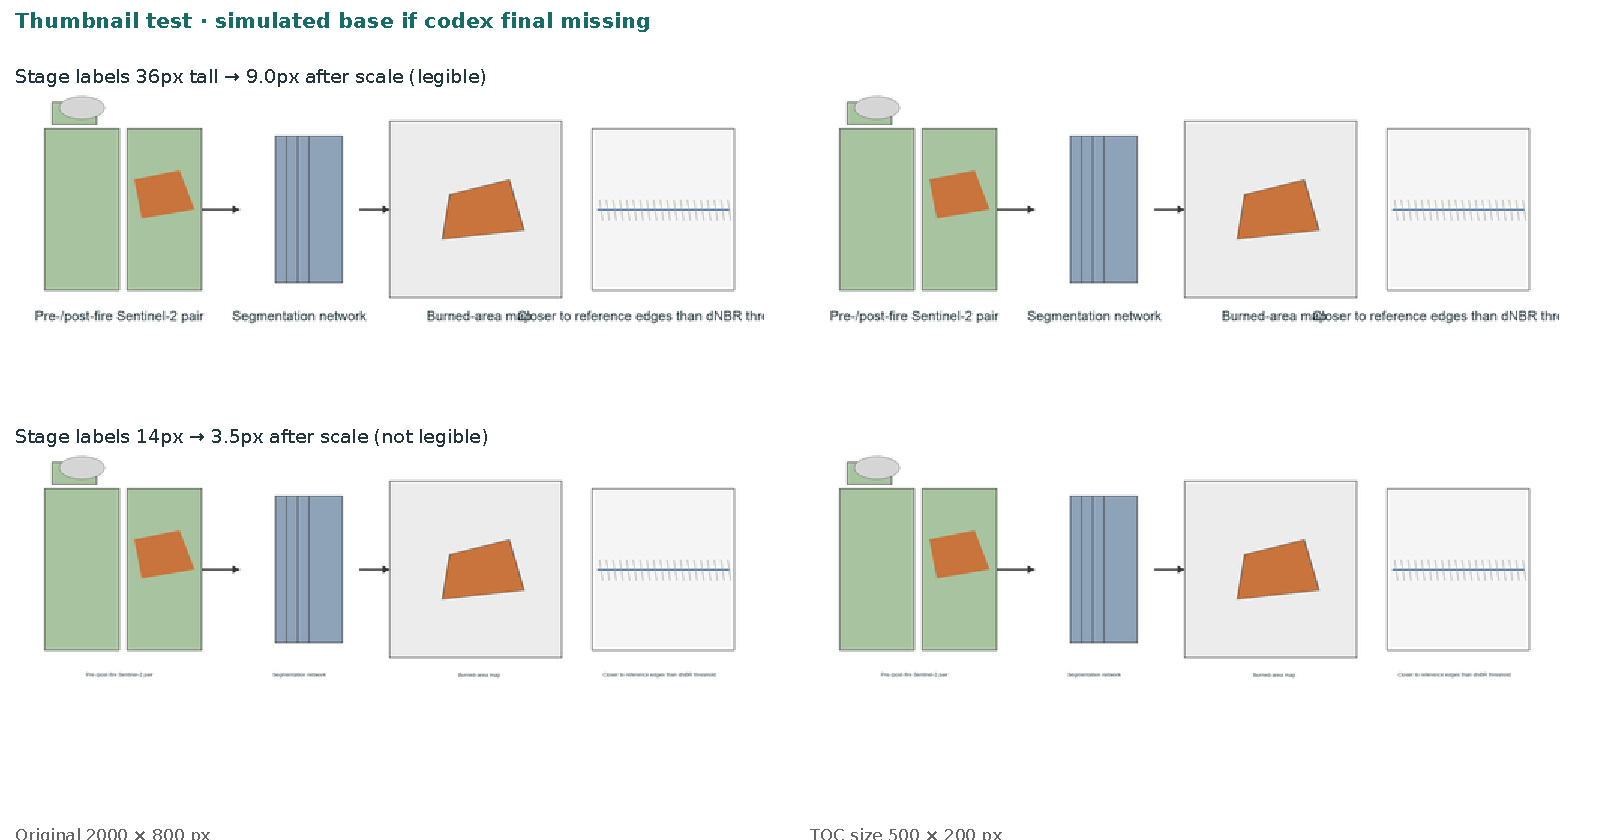
\includegraphics[width=\linewidth]{figures/ch10/ch10-07-thumbnail-test-en.pdf}
\caption{Thumbnail test. The graphical abstract scaled to about $200\ \text{px}$ high---the TOC display height mentioned in Elsevier's guidelines---shown at actual pixels (tested here on the same $2000 \times 800\ \text{px}$ simulated layout base while varying only stage-label font height). Top: stage names at $36\ \text{px}$ height scale to $9.0\ \text{px}$ and remain legible. Bottom: the same image with $14\ \text{px}$ stage names scales to $3.5\ \text{px}$ and becomes unreadable. The limits line is small in the thumbnail but readable on the article page.}\label{fig:ch10-07}
\end{figure}

\section{Walk-Through of the Complete Chapter Case}

In this chapter case, we started from a fictional teaching abstract and completed journal rule verification (Figure~\ref{fig:ch10-01}), four-line contribution card distillation (Table~\ref{tab:ch10-02-card}), PDF-to-prompt boundary auditing (Figure~\ref{fig:ch10-02}, Table~\ref{tab:ch10-03-compare}), A/B composition comparison (Figures~\ref{fig:ch10-03} and \ref{fig:ch10-04}, Table~\ref{tab:ch10-04-ab}), over-claim counter-example deconstruction (Figure~\ref{fig:ch10-05}, Table~\ref{tab:ch10-05-overclaim}), final base refinement and TikZ vector lettering (Figure~\ref{fig:ch10-06}), and the $200\ \text{px}$ thumbnail test (Figure~\ref{fig:ch10-07}). The nine pre-delivery verification checks are recorded in Table~\ref{tab:ch10-07-verify}.

\begin{table}[htbp]\centering\footnotesize
\setlength{\tabcolsep}{3pt}
\renewcommand{\arraystretch}{1.15}
\caption{Nine-item verification table (C1--C9) for the final teaching-case graphical abstract (Figure~\ref{fig:ch10-06}).}\label{tab:ch10-07-verify}
\begin{tabularx}{\linewidth}{@{}c>{\raggedright\arraybackslash}p{26mm}>{\raggedright\arraybackslash}p{32mm}Y@{}}
\toprule
\textbf{\#} & \textbf{Check item} & \textbf{Verification method} & \textbf{Recorded result} \\
\midrule
C1 & All four contribution-card rows in figure & Point to the element for each row & Question and Method map to Stages (1)--(3) and T1--T4; Finding maps to Stage (4) and T5; Limits map to upper-left cloud tile and bottom T6 phrase \\
C2 & No elements beyond the paper & Translate each icon into a sentence and check against abstract & All objects match the brief's schematic elements; no flames, globes, alarm clocks, or percentage numbers \\
C3 & No numbers, data plots, or photo-textured imagery & Zoom check of textures and graphic categories & No numbers or data plots; map tiles are flat schematics (fills have slight tonal variation; caption states ``not real satellite data'') \\
C4 & Aspect ratio and pixels & Check file properties: $5:2$, $\ge 1328 \times 531\ \text{px}$ & Delivered base art is $2000 \times 800\ \text{px}$, meeting the $5:2$ ratio and pixel floor \\
C5 & Thumbnail legibility & Figure~\ref{fig:ch10-07} test: stage names legible at $200\ \text{px}$ height & Stage names set at $\approx 36\ \text{px}$ height scale to $\approx 9.0\ \text{px}$ at $200\ \text{px}$ height and remain recognizable \\
C6 & No pseudo-text in base art & Full-size zoom inspection & Selected base image shows no letters, digits, or pseudo-text (earlier counter-example runs with dial digits and ticks were rejected) \\
C7 & Chinese and English editions differ only in text layer & Compare base-image file hashes & Both editions share the same text-free base file and switch only the TikZ text layer per Table~\ref{tab:ch10-06-text} \\
C8 & Journal rules re-checked before submission & Log target journal URL and access date & Logged Elsevier general guidelines URL and October 2026 access date; re-verify on the target journal page before upload \\
C9 & PDF-to-prompt scope and raw output archived & Check local figure archive records & When using \sdtool{graphical-abstract-maker}, archive the 5-page scope, verbatim prompt, and comparison table together \\
\bottomrule
\end{tabularx}
\end{table}

\section{What AI Can and Cannot Do at This Stage}

The division of labor between AI tools and the author across graphical-abstract production is summarized in Table~\ref{tab:ch10-08-ai}.

\begin{table}[htbp]\centering\footnotesize
\setlength{\tabcolsep}{3pt}
\renewcommand{\arraystretch}{1.15}
\caption{What AI can do, what AI cannot do, and what the author must verify when making a graphical abstract.}\label{tab:ch10-08-ai}
\begin{tabularx}{\linewidth}{@{}>{\raggedright\arraybackslash}p{18mm}YYY@{}}
\toprule
\textbf{Stage} & \textbf{What AI (\scidraw{}, etc.) can do} & \textbf{What AI cannot do} & \textbf{What the author must verify} \\
\midrule
Reading paper & Graphical-abstract tool reads first 5 PDF pages ($\le 6{,}000$ chars) and drafts a $60\text{--}110$-word visual prompt & Understand full paper; decide which finding matters most; guarantee scope limits are kept & Log reading scope and raw output; compare line by line with contribution card and restore limits \\
Distilling contribution & Shorten abstract sentences; list candidate visual objects & Decide core contribution; judge whether claim strength matches evidence & Check that every row maps to a source sentence and verbs like ``improves,'' ``solves,'' or ``predicts'' do not overreach \\
Composition & Generate multiple candidates of one layout; generate a second layout on request & Propose reasoned alternative layouts and explain trade-offs automatically (batch outputs are random variants) & Write two layouts explicitly; compare by ratio, reading path, thumbnail legibility, and limit visibility \\
Base generation & Flat schematic style, text-free base art, empty bands (with stochastic variation) & Guarantee no pseudo-text, exact coordinates, or that schematic tiles are not read as real data & Zoom to check for pseudo-text; keep imagery schematic and state ``not real data'' in caption \\
Revision & Modify using a prior image as reference per instructions & Lock objects; guarantee only target spot changes & Re-run full verification after each edit (see Chapter 11) \\
Text & (Not recommended) generate text in image & Reliable spelling and alignment & Overlay text in TikZ or layout software; proofread word by word \\
Delivery & Export image files & Know target journal's current rules & Check target journal's live page for ratio, pixels, fonts, and format; log date and run thumbnail test \\
Integrity & --- & Judge whether an icon is an over-claim & Translate every element into a sentence and verify its basis in the paper \\
\bottomrule
\end{tabularx}
\end{table}

\section{Chapter Checklist}

\begin{itemize}
\item Opened the target journal's \textbf{current} graphical-abstract page and logged the URL, access date, ratio, pixel floor, fonts, and file formats.
\item Verified that all four contribution-card rows (Question / Method / Finding / Limits) map to original sentences in the paper without inflating claim strength.
\item If PDF-to-prompt was used: archived the reading scope (first 5 pages) and raw output, compared line by line with the contribution card, and restored the limits.
\item Created at least two \textbf{explicitly reasoned} composition candidates and selected between them by aspect ratio, reading start and end points, thumbnail legibility, and limit placement.
\item Confirmed that every icon translates into a sentence supported by the paper, with no flames, globes, alarm clocks, or standalone numbers claiming more than proved.
\item Kept schematic imagery free of photorealistic texture; if real imagery is used, documented source, license, and processing.
\item Checked that base art contains no pseudo-text, overlaid all labels in a vector layer, proofread every word, and kept total word count low.
\item Verified that stage names remain legible and reading order stays clear at TOC thumbnail height (such as $200\ \text{px}$ high).
\item Confirmed that Chinese and English editions differ only in the overlaid text layer.
\item Logged tools, prompts, generation counts, and manual edits in the figure archive.
\end{itemize}

\section{Exercises}

\begin{enumerate}
\item \textbf{(Contribution card: pen and paper.)} Pick a recent paper in your field, read only the abstract and conclusion, and write a four-line contribution card; then read the full Results section and revise the ``Finding'' and ``Limits'' rows. Compare the two versions and identify which phrasing in the first version would have produced an over-claim in a graphical abstract.
\item \textbf{(Hands-on with \scidraw{}: comparing PDF-to-prompt output.)} Upload the PDF of your own paper (or the paper from Exercise 1) to \scidraw{}'s graphical-abstract tool (\sdtool{graphical-abstract-maker}) and save the returned visual prompt. Build a comparison table recording whether each row of your contribution card was ``preserved,'' ``dropped,'' or ``inflated.'' Write a revised generation prompt, generate a candidate image, and complete the Chapter Checklist.
\item \textbf{(Changing format.)} Adapt this chapter's final graphical abstract ($5:2$) to a $1200 \times 1200\ \text{px}$ square format: sketch the layout, explain whether you would fold Candidate A into two rows or use Candidate B's central figure, show where the scope limits would sit, and explain how the thumbnail test should be adjusted.
\end{enumerate}

\section*{References}

\begin{itemize}
\item American Chemical Society. \textit{The Journal of Organic Chemistry} Author Guidelines. \url{https://researcher-resources.acs.org/publish/author_guidelines?coden=joceah} (accessed 2026-10-29).
\item American Chemical Society. \textit{Langmuir} Author Checklist. \url{https://pubs.acs.org/page/langd5/submission/author-checklist} (accessed 2026-10-29).
\item Cell Press. Attract readers at a glance with your Graphical Abstract. \url{https://crosstalk.cell.com/blog/attract-readers-at-a-glance-with-your-graphical-abstract} (accessed 2026-10-29).
\item Cell Press. \textit{Cell Reports} Final File Requirements. \url{https://www.cell.com/pb-assets/journals/EM/MasterFFCs/CELREPFFC-1750868285900.pdf} (accessed 2026-10-29).
\item Chuvieco E, Mouillot F, van der Werf GR, et al. Historical background and current developments for mapping burned area from satellite Earth observation. \textit{Remote Sensing of Environment}. 2019;225:45--64. \url{https://doi.org/10.1016/j.rse.2019.02.013}
\item Elsevier. Graphical abstracts --- Author tools and resources. \url{https://www.elsevier.com/researcher/author/tools-and-resources/graphical-abstract} (accessed 2026-10-29).
\item Giglio L, Boschetti L, Roy DP, Humber ML, Justice CO. The Collection 6 MODIS burned area mapping algorithm and product. \textit{Remote Sensing of Environment}. 2018;217:72--85. \url{https://doi.org/10.1016/j.rse.2018.08.005}
\item Ibrahim AM, Lillemoe KD, Klingensmith ME, Dimick JB. Visual abstracts to disseminate research on social media: a prospective, case-control crossover study. \textit{Annals of Surgery}. 2017;266(6):e46--e48. \url{https://doi.org/10.1097/SLA.0000000000002277}
\item Knopp L, Wieland M, R\"attich M, Martinis S. A deep learning approach for burned area segmentation with Sentinel-2 data. \textit{Remote Sensing}. 2020;12(15):2422. \url{https://doi.org/10.3390/rs12152422}
\item Pferschy-Wenzig E-M, Pferschy U, Wang D, Mocan A, Atanasov AG. Does a graphical abstract bring more visibility to your paper? \textit{Molecules}. 2016;21(9):1247. \url{https://doi.org/10.3390/molecules21091247}
\item Roy DP, Huang H, Boschetti L, et al. Landsat-8 and Sentinel-2 burned area mapping --- a combined sensor multi-temporal change detection approach. \textit{Remote Sensing of Environment}. 2019;231:111254. \url{https://doi.org/10.1016/j.rse.2019.111254}
\end{itemize}

% TODO: 1) Live test output from uploading `teaching-paper.pdf` to SciDraw AI `/graphical-abstract-maker` (`provenance/ch10/pdf-prompt.txt`) remains to be captured and archived;
% TODO: 2) `figures/ch10/ch10-07-thumbnail-test-en.pdf` currently uses the script's built-in simulated base art (`simulated_base: true`); regenerate after wiring in the composited `ch10-06-final-base.png` final figure;
% TODO: 3) The main Cell Press figure guidelines page (`https://www.cell.com/figureguidelines`), previously blocked by access verification, and the ACS general graphics guideline clause on minimum 8 pt type remain to be manually verified against the original web pages.

\chapter{From ``Make It Nicer'' to Executable Revisions}
\usetikzlibrary{decorations.pathmorphing}

Chen, a master's student in civil engineering, was writing Chapter 2 (Methods) of his thesis and needed a system architecture schematic for a structural health monitoring (SHM) sensor network on a cable-stayed bridge. The diagram had to show where sensors sit on the structure, how wireless nodes forward measurements to an on-site gateway, how the cloud subsystem processes the incoming streams, and how early-warning alerts reach bridge operators. Half an hour after emailing his first draft to his advisor, he received a one-line reply: ``Make it a bit nicer---it looks messy right now and not professional enough.''

Chen immediately reopened his image generator, swapped the white background for a dark-blue ``high-tech'' gradient, added three-dimensional drop shadows to the pylons, and surrounded the sensors with glowing cyan radio ripples. When he sent the second version back, his advisor still shook his head. For the third version, hoping to ``clean up the clutter,'' Chen prompted the tool to ``make the messy wireless signal lines cleaner.'' While redrawing the canvas, the generative model quietly erased one stay cable and the satellite positioning antenna atop the right pylon. Because Chen stared only at the newly restyled dashed wireless lines, he missed both omissions---until a senior labmate pointed them out on the projector screen during their weekend group meeting.

Jumping straight into cosmetic regeneration after receiving vague feedback, and inspecting only the edited spot after a local revision, are the two main reasons scientific figures go through endless rounds of rework or lose details that were originally right. This chapter addresses both pitfalls. You will learn how to translate vague aesthetic impressions into a prioritized, location-specific revision sheet; how to divide labor between generative image models and deterministic layout layers; and how to use full-figure re-verification and version trees to catch collateral changes when a local prompt alters the rest of the image.

\section{Three Levels of Issues: First Accurate, Then Clear, Finally Consistent}

When a draft figure comes back from an advisor, co-author, or reviewer covered in casual remarks, the worst strategy is to fix items in the order they were spoken. Some authors spend two hours adjusting fonts and palettes only to realize a process arrow points the wrong way; others regenerate an entire diagram to make the style ``pop,'' corrupting component counts that had already been verified.

To make revision converge, classify every flaw into one of three levels and resolve them strictly from top to bottom: \textbf{first scientific errors, then reading obstacles, and finally visual consistency} (Figure~\ref{fig:ch11-01}).

\begin{figure}[htbp]\centering
\resizebox{\linewidth}{!}{% FIG ch11-01 three levels (English)
\usetikzlibrary{arrows.meta,positioning,calc}
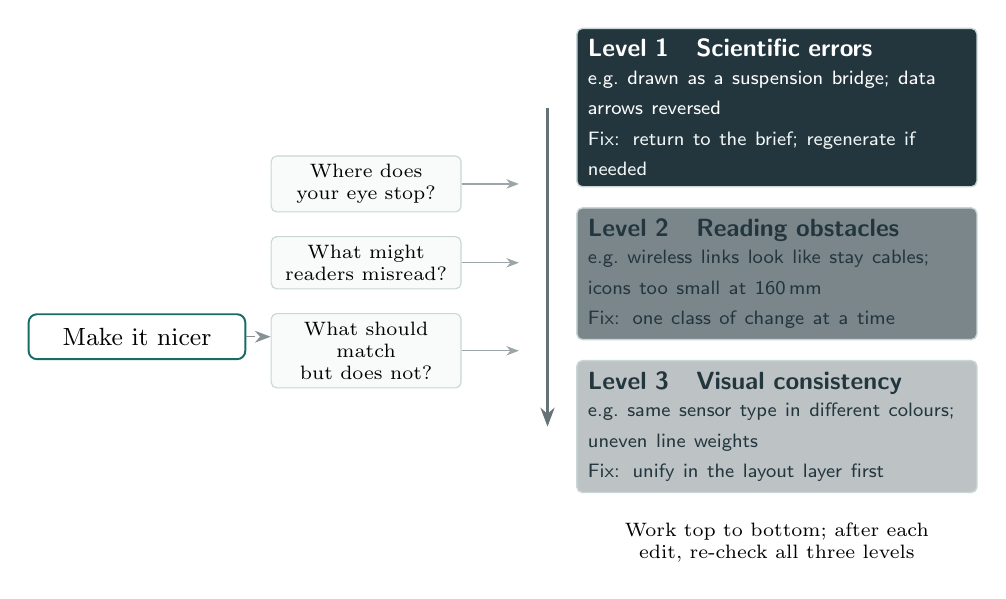
\begin{tikzpicture}[x=\linewidth/100,y=\linewidth/100]
\begin{scope}[
  font=\sffamily\small,
  level/.style={
    draw=BookRule, line width=0.5pt, rounded corners=2pt,
    minimum width=50mm, minimum height=15mm, align=left, inner sep=4pt,
    text width=48mm, anchor=west,
  },
  qbox/.style={
    draw=BookRule, fill=BookPale!40, rounded corners=2pt,
    align=center, inner sep=3pt, text width=22mm, font=\scriptsize,
  },
]
  \node[
    draw=BookTeal, line width=0.7pt, fill=white, rounded corners=3pt,
    align=center, inner sep=5pt, text width=24mm, font=\small,
  ] (bubble) at (8,42) {Make it nicer};
  \draw[BookInk!55, dashed, -{Stealth[length=2mm]}] (bubble.east) -- (22,42);

  \node[qbox] (q1) at (32,58) {Where does\\your eye stop?};
  \node[qbox, below=3mm of q1] (q2) {What might\\readers misread?};
  \node[qbox, below=3mm of q2] (q3) {What should match\\but does not?};

  \foreach \q in {q1,q2,q3} {
    \draw[BookInk!45, -{Stealth[length=1.6mm]}] (\q.east) -- ++(6,0);
  }

  \node[level, fill=BookInk, text=white] (L1) at (54,66) {%
    \textbf{Level 1\quad Scientific errors}\\[-1pt]
    {\scriptsize e.g.\ drawn as a suspension bridge; data arrows reversed}\\
    {\scriptsize\textcolor{BookPale!90}{Fix: return to the brief; regenerate if needed}}};
  \node[level, fill=BookInk!60, text=BookInk, below=2.5mm of L1] (L2) {%
    \textbf{Level 2\quad Reading obstacles}\\[-1pt]
    {\scriptsize e.g.\ wireless links look like stay cables; icons too small at 160\,mm}\\
    {\scriptsize Fix: one class of change at a time}};
  \node[level, fill=BookInk!30, text=BookInk, below=2.5mm of L2] (L3) {%
    \textbf{Level 3\quad Visual consistency}\\[-1pt]
    {\scriptsize e.g.\ same sensor type in different colours; uneven line weights}\\
    {\scriptsize Fix: unify in the layout layer first}};

  \coordinate (ordA) at ($(L1.west)+(-3,0)$);
  \coordinate (ordB) at ($(L3.west)+(-3,0)$);
  \draw[BookInk!70, line width=0.8pt, -{Stealth[length=2.4mm]}] (ordA) -- (ordB);
  \node[font=\scriptsize, align=center, text width=46mm, anchor=north]
    at ($(L3.south)+(0,-2.5mm)$) {Work top to bottom; after each edit, re-check all three levels};
\end{scope}
\end{tikzpicture}
}
\caption{Splitting vague feedback into three levels. Fix scientific errors first, then reading obstacles, then visual consistency. After every change, re-check from the top: a generative edit can alter the whole image.}\label{fig:ch11-01}
\end{figure}

\textbf{Level 1 comprises scientific errors (things drawn incorrectly).} Whenever an object, count, spatial location, connection topology, or process direction contradicts study facts or domain conventions, it is a Level 1 flaw. In our bridge monitoring schematic, if the thesis studies a twin-pylon cable-stayed bridge (where inclined stay cables run directly from pylons to the deck girder), drawing a suspension bridge with catenary main cables and vertical hangers---or a six-pylon perspective highway bridge---misrepresents the structure. If stay cables plunge into the water or ground rather than anchoring to the deck girder, the load-transfer mechanics are wrong. If the cup anemometer sits under the deck girder or low on a pier instead of in open airflow atop a pylon, its placement violates instrumentation practice. If data arrows point backward from the cloud to the sensors, or jump directly from deck sensors to a smartphone alarm while bypassing data aggregation, feature extraction, and engineering review, the diagram states a false mechanism---implying that raw sensors diagnose damage autonomously. Misspelled technical terms, or fabricated waveforms and a ``Health Index 92\%'' gauge inside a methods schematic with no empirical data, are also Level 1 errors: every word, number, and curve makes a scientific claim.

\textbf{Level 2 comprises reading obstacles (nothing is factually wrong, but readers struggle to find or decode the message).} These flaws do not falsify the science, yet poor composition, tangled paths, cramped scale, or ambiguous line styles hinder rapid comprehension (Rougier et al., 2014; Wong, 2011a). Four reading obstacles recur in AI drafts: (1) \textbf{visual noise overwhelming the subject}, such as sunset skies, city skylines, and water reflections shrinking sensor nodes into tiny specks; (2) \textbf{visual collisions between distinct categories}, such as drawing wireless links from sensors to the gateway at nearly the same weight and angle as stay cables so readers cannot tell steel cables from radio signals; (3) \textbf{folded reading paths}, such as placing the gateway above the cloud when the brief specifies a bottom-to-top upload path, forcing the eye to double back; and (4) \textbf{illegibility at print scale}, where scaling to a full-page width ($160\ \text{mm}$) shrinks sensor icons below $2\ \text{mm}$ and text below $6\ \text{pt}$.

\textbf{Level 3 comprises visual consistency issues (items of the same class look different).} Once scientific content is accurate and the reading path is clear, the final pass unifies visual conventions: rendering all five accelerometers in the same blue; removing a red liquid column inside a thermometer icon when red is reserved exclusively for the final alert arrow (Wong, 2011b); eliminating residual shading gradients in a flat 2D schematic; and matching line weights and box alignments inside the cloud subsystem.

Two operational rules explain why you must enforce $\text{Level 1} \rightarrow \text{Level 2} \rightarrow \text{Level 3}$:

First, \textbf{upper-level changes invalidate lower-level polish.} When a draft has three or more Level 1 scientific errors, the fastest path is never to patch the image in place, but to return to the figure brief, rewrite the input, and regenerate the base art. Time spent tuning colors or aligning boxes on the wrong bridge type or reversed arrows is wasted when the base image is replaced.

Second, \textbf{every generative edit can perturb the entire canvas.} Unlike selecting a single rectangle in a vector editor, sending a bitmap back into an image model resamples the whole image. If you unify Level 3 colors first and then ask the model to fix Level 2 layout or Level 1 cable counts, the unified colors and icons often drift again during resampling. Lock down Level 1 structure and Level 2 spatial paths first, then delegate Level 3 color codes, line weights, and typography to a deterministic layout layer (TikZ or vector software).

\section{Translating Vague Feedback into Specific Issues}

In research collaboration, reviewers usually offer a three-second impression: ``It looks cluttered,'' ``The focus isn't clear,'' or ``Make it more professional.'' Typing ``make it cleaner and more professional'' into a prompt box delegates diagnosis to an algorithm that does not know your project. Instead, use \textbf{three follow-up questions} (Figure~\ref{fig:ch11-01}) to translate impressions into location-specific observations:

\begin{enumerate}
\item \textbf{Question 1: ``Where did your eye get stuck, or what pulled your attention first?''} Isolates Level 2 reading obstacles. If the reply is ``I looked straight at the right-hand dashboards and sunset skyline and couldn't find the bridge sensors,'' the issue becomes: \emph{Realistic scenery and decorative panels dominate the frame, while sensor icons are too small.}
\item \textbf{Question 2: ``If a peer outside our project looked only at this figure, what would they most likely misread?''} Uncovers Level 1 scientific errors and ambiguous links. If the reply is ``They'd think the system outputs a 92\% health score automatically, and confuse orange diagonal lines with stay cables,'' the fix becomes: \emph{Delete fabricated health scores and waveforms; make wireless links thick short-dashed lines with wave marks.}
\item \textbf{Question 3: ``Which two elements should look the same but do not, or differ in meaning yet look too similar?''} Targets Level 3 consistency and encoding conflicts. If the reply is ``Every sensor on the bridge is the same white box, so I must read tiny text to know its type,'' the fix becomes: \emph{Remove callout boxes and assign each of the six sensor types a distinct shape and color.}
\end{enumerate}

Even when you cannot interview the reviewer in person, you can run four structured self-checks on any draft to perform the same translation yourself: (1) \textbf{roll-call audit against the brief}, counting every object and tracing every arrow against your object and relation tables; (2) \textbf{full-scale print-width inspection} at the exact target width (e.g., $160\ \text{mm}$), checking whether every icon is $\ge 2\ \text{mm}$ and every label is $\ge 6\ \text{pt}$; (3) \textbf{grayscale conversion} (Wong, 2011b) to verify that distinct link types remain separable by dash pattern and stroke weight alone; and (4) \textbf{a 30-second closed-screen recall test}, asking a labmate outside your subtopic to view the draft for 30 seconds and explain the architecture from memory.

Let us walk through this diagnostic process using our chapter's main case study. \textbf{Note on the case study:} This example is a \emph{simplified teaching scenario}. It illustrates the system architecture of a structural health monitoring (SHM) sensor network on a twin-pylon cable-stayed bridge based on generic textbook and review-level conventions; it does not represent the monitoring deployment of any real bridge and reports no empirical measurements or damage-identification results.

In structural engineering, SHM systems track structural condition over time by deploying sensors across key components, extracting damage-sensitive features from measured responses, and comparing those features against a baseline; because environmental and operational variations such as temperature gradients, wind loading, and live traffic also shift vibration and strain features, an SHM system must measure those factors concurrently so normal operational changes are not mistaken for structural damage (Farrar and Worden, 2007). Long-span bridge monitoring systems typically integrate accelerometers (measuring deck, pylon, and stay-cable vibrations), strain gauges, anemometers, temperature sensors, displacement transducers at expansion joints or bearings, and Global Navigation Satellite System (GNSS) antennas, coupled with data acquisition, transmission, processing, and management subsystems (Ko and Ni, 2005). Wireless sensor networks reduce the high cost of running long cables across a bridge, though practical deployments must manage constraints on bandwidth, time synchronization, and power supply, often combining wired backbones with wireless subnetworks (Lynch and Loh, 2006; Kim et al., 2007). Our teaching scenario models wireless sensor nodes forwarding data to an on-site gateway and enforces a critical domain principle: \textbf{an early-warning alert notifies bridge operators when extracted features cross a threshold or exhibit an anomaly, triggering manual inspection and engineering review---it is not an automated diagnosis of structural damage.}

Consider what happened when Chen skipped writing a figure brief and submitted a single vague sentence to the image model:

\begin{Prompt}
Create a beautiful, professional illustration of a smart structural health
monitoring system for a bridge with sensors, wireless network, cloud and alerts.
Landscape, aspect ratio 2:1.
\end{Prompt}

Figure~\ref{fig:ch11-02} shows the first-attempt output from that one-line prompt. Applying our three diagnostic questions and four self-checks turns the advisor's remark---``a bit messy and not professional enough''---into the nine location-specific issues marked on the image and cataloged in Table~\ref{tab:ch11-01}.

\begin{figure}[htbp]\centering
\begin{tikzpicture}
\definecolor{Ch11IssueRed}{HTML}{C0392B}
\node[anchor=south west,inner sep=0] (img) at (0,0) {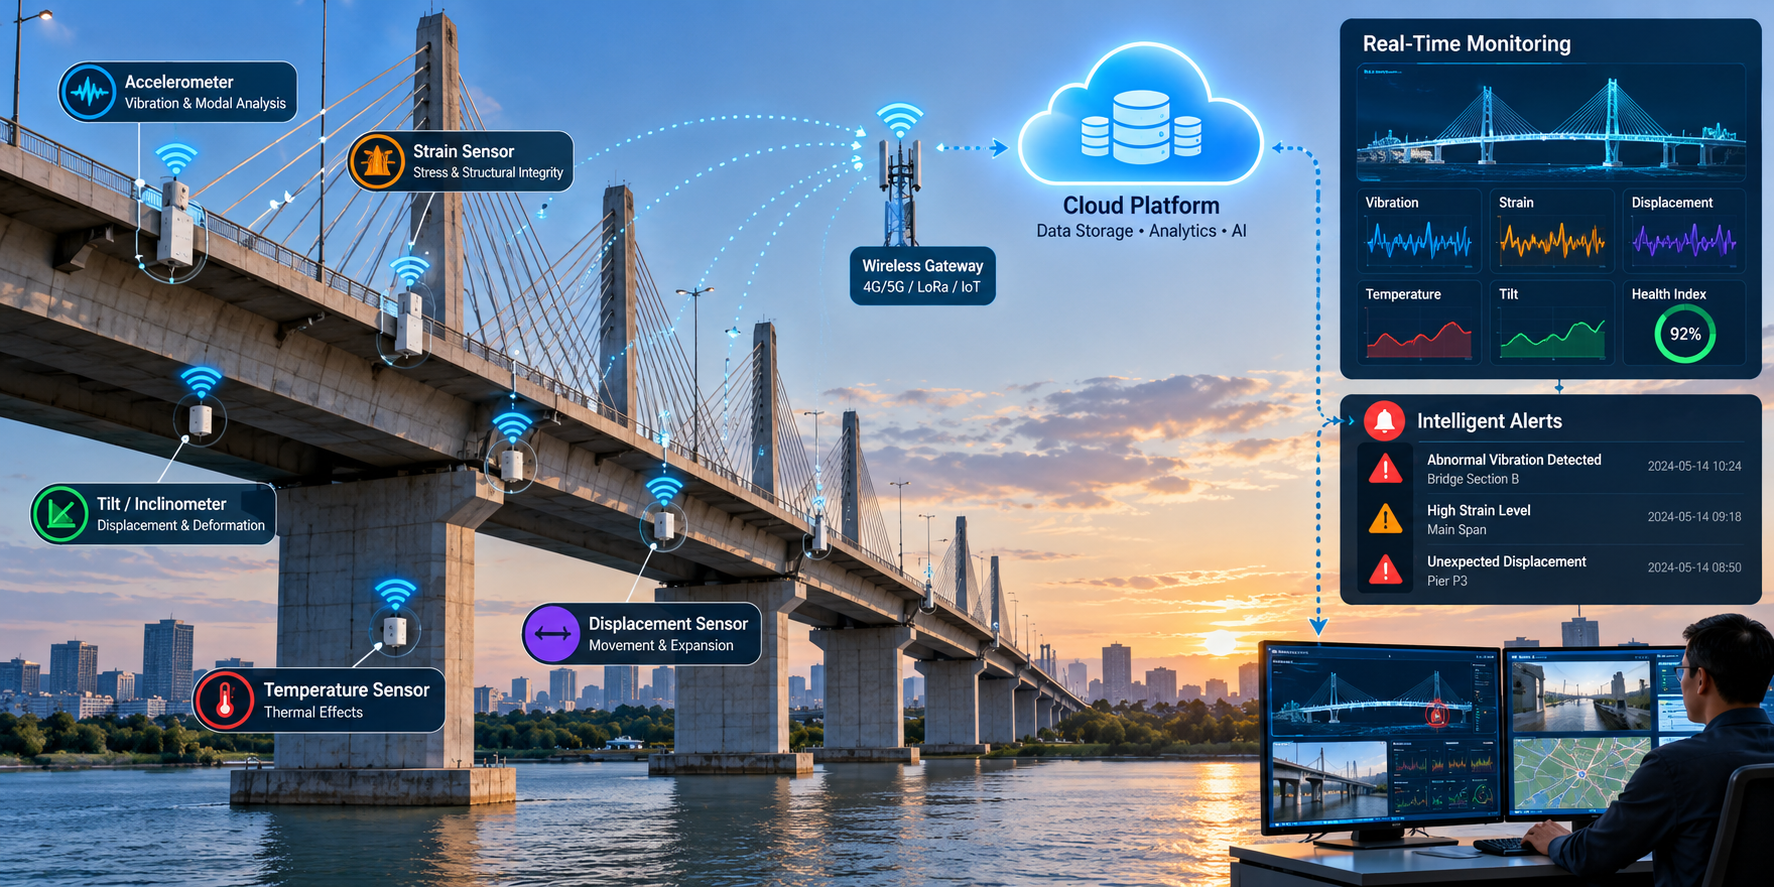
\includegraphics[width=\linewidth]{figures/ch11/ch11-02-v1-vague.png}};
\begin{scope}[x={(img.south east)},y={(img.north west)}]
  \tikzset{issuemark/.style={draw=Ch11IssueRed,line width=0.9pt,rounded corners=2pt,fill=white,fill opacity=0.90,text opacity=1,text=Ch11IssueRed,font=\sffamily\bfseries\scriptsize,inner sep=1.5pt}}
  \node[issuemark] at (0.35,0.62) {S1};
  \node[issuemark] at (0.24,0.82) {S2};
  \node[issuemark] at (0.55,0.84) {S3};
  \node[issuemark] at (0.95,0.64) {S4};
  \node[issuemark] at (0.78,0.44) {S5};
  \node[issuemark] at (0.64,0.76) {S6};
  \node[issuemark] at (0.62,0.28) {R1};
  \node[issuemark] at (0.64,0.91) {R2};
  \node[issuemark] at (0.11,0.56) {V1};
\end{scope}
\end{tikzpicture}
\caption{First draft from a one-line prompt (counter-example). Numbers match the issue list in Table~\ref{tab:ch11-01}: S1--S6 for scientific errors, R1--R2 for reading obstacles, and V1 for visual consistency. With more than three scientific errors, the first item on the revision sheet is to rewrite the input, not to patch this image. Base art and any text in it were generated by an image model and not checked.}\label{fig:ch11-02}
\end{figure}

\begin{table}[htbp]\centering\scriptsize
\setlength{\tabcolsep}{3pt}
\renewcommand{\arraystretch}{1.08}
\caption{Decomposing ``a bit messy and not professional enough'' in Figure~\ref{fig:ch11-02} into nine concrete issues across three levels.}\label{tab:ch11-01}
\begin{tabularx}{\linewidth}{@{}c>{\raggedright\arraybackslash}p{16mm}>{\raggedright\arraybackslash}p{21mm}YY@{}}
\toprule
\textbf{ID} & \textbf{Level} & \textbf{Location} & \textbf{Observed phenomenon} & \textbf{Why it is a problem} \\
\midrule
S1 & Scientific error & Bridge form & Drawn as a 6-pylon 3D perspective cable-stayed bridge rather than a twin-pylon 2D side view & Contradicts the twin-pylon study structure and 2D engineering elevation conventions \\
S2 & Scientific error & Bridge sensors & Only 5 callout boxes; pylon-top anemometer and GNSS missing; strain gauge points to upper cables instead of deck soffit; thermometer low on pier & Incomplete sensor inventory (cannot map to 12 required nodes) and placements violate engineering practice \\
S3 & Scientific error & Gateway--cloud link & Blue dashed line between wireless gateway and cloud platform has arrowheads at both ends & Misrepresents unidirectional data upload as an ambiguous bidirectional link \\
S4 & Scientific error & Top-right panel & Shows five fabricated waveform traces and a ``Health Index 92\%'' circular gauge & Methods schematic contains no empirical data, and SHM does not yield a single ``92\%'' score \\
S5 & Scientific error & Mid-right alert box & Lists three dated alarms for ``2024-05-14'' (Section B vibration, main-span high strain, Pier P3 displacement) & Fabricates monitoring dates, pier labels, and anomaly events absent from the study \\
S6 & Scientific error & Baked-in text & Titles, protocol names, and numbers are rasterized directly into the bitmap & Labels are scientific content; locking them into pixels prevents editing or translation \\
R1 & Reading obstacle & Scene \& lower right & Sunset, city skyline, river reflections, and a dual-monitor operator scene fill over half the frame & Photorealistic scenery and decorative UI panels drown out the sensing architecture \\
R2 & Reading obstacle & Cloud interior & Cloud contains only a database cylinder and generic ``Data Storage $\cdot$ Analytics $\cdot$ AI'' text & Omits the 3 explicit steps (cleaning $\rightarrow$ feature extraction $\rightarrow$ threshold/anomaly check) \\
V1 & Visual consistency & Sensors vs.\ badges & All bridge nodes are identical white boxes, while callouts use 5 colored circles & Sensor icons on the bridge lack shape and color coding, requiring text to tell types apart \\
\bottomrule
\end{tabularx}
\end{table}

This initial draft contains six Level 1 scientific errors alone (S1--S6). \textbf{Whenever a draft exhibits three or more Level 1 scientific errors, the first action on your revision sheet is never to patch the image in place---it is to return to the figure brief and regenerate from scratch.}

\section{Writing a Revision Sheet: One Change per Item}

Before generating our structural baseline image (V2), we define the components, sensor counts, and transmission links as a verifiable acceptance baseline (Table~\ref{tab:ch11-02}).

\begin{table}[htbp]\centering\scriptsize
\setlength{\tabcolsep}{3pt}
\renewcommand{\arraystretch}{1.08}
\caption{Object and relation inventory for the cable-stayed bridge SHM schematic (acceptance baseline from V2 onward).}\label{tab:ch11-02}
\begin{tabularx}{\linewidth}{@{}l>{\raggedright\arraybackslash}p{24mm}c>{\raggedright\arraybackslash}p{33mm}Y@{}}
\toprule
\textbf{ID} & \textbf{Object / relation} & \textbf{Count} & \textbf{Location (side view)} & \textbf{Visual \& line convention (text-free base)} \\
\midrule
B1--B2 & Deck girder \& pylons & 1, 2 & Left $70\%$; pylons at $x\approx 0.22, 0.50$ & Light-gray horizontal girder; medium-gray vertical single-column pylons \\
B3 & Stay cables & 16 & 4 left and 4 right per pylon, fanning from upper pylon to deck & Thin dark-gray straight lines; all connect pylon to deck, none touching water or ground \\
B4--B5 & Piers \& water band & 4, 1 & Foundations under pylons + two end piers; bottom water zone & Gray pier supports; pale-blue horizontal water band \\
S1--S5 & Accelerometers & $3+2$ & Main-span deck at $1/4, 1/2, 3/4$ (3) + midpoint of longest outer cables (2) & Small blue squares (each with a tiny black dot beside it representing wireless node N) \\
S6--S7 & Strain gauges & 2 & Underside of deck at mid-main span and next to left pylon & Small green rectangles \\
S8 / S9 & Anemometer / GNSS & 1 / 1 & Top of left pylon (S8) / top of right pylon (S9) & Small cup-anemometer icon / small dish-antenna icon \\
S10 / S11--S12 & Thermometer / displacement & $1 / 2$ & Left side-span deck (1) / both deck-end expansion joints (2) & Small round thermometer icon / small purple squares \\
G / C / P / D & Gateway / cloud / steps / terminal & 1/1/3/1 & Right $30\%$ data-path zone & Right-bank cabinet with antenna (G); cloud with server bars and 3 serial empty boxes (C, P); far-right monitor + phone (D) \\
L1 & Wireless links & Multiple & Sensor nodes N $\rightarrow$ gateway G & Short orange dashed lines with wave marks, clearly distinct from stay cables \\
L2 / L3 / L4 & Upload / steps / alert & 1 / 2 / 1 & G$\rightarrow$C / between P boxes / last P box$\rightarrow$D & Solid orange arrow / small dark-gray arrows / solid red arrow (only red element in figure) \\
\bottomrule
\end{tabularx}
\end{table}

In the \scidraw{} Scientific Figure Workflow wizard (\sdtool{figure-workflow}), we select the ``Mechanism and Workflow Diagrams'' track, populate the template with the following brief, download a copy, and generate the base image in the workflow diagram generator (\sdtool{workflow-diagram-generator}) or prompt drawing tool (\sdtool{ai-drawing}):

\begin{Prompt}
[Purpose & Audience] System schematic for Chapter 2 (Methods) of a civil engineering
master's thesis; full-page print width ~160 mm for structural engineering peers.
[Goal] Show where 12 sensors of 6 types sit on a twin-pylon cable-stayed bridge, how
wireless nodes forward data to an on-site gateway and cloud analytics pipeline, and
how threshold/anomaly alerts reach operators for engineering review.
[Basis] Farrar & Worden 2007; Ko & Ni 2005; Lynch & Loh 2006. Simplified teaching
architecture, not a real bridge, containing no empirical monitoring data.
[Objects] See inventory B1-B5, S1-S12, G, C, P, D: twin pylons, 16 stay cables (4 per
side of each pylon), 12 sensors (same type = same shape and color) with black node dots.
[Relations] L1 wireless: short orange dashed lines with wave marks (sensor -> gateway),
distinct from gray stay cables; L2 upload: solid orange arrow (gateway -> cloud);
L3 processing: 2 dark-gray arrows across 3 cloud boxes; L4 alert: solid red arrow
(last box -> terminal; red used nowhere else).
[Layout & Style] Landscape 2:1, flat 2D schematic on white, no 3D or gradients. Left
70% bridge elevation; right 30% gateway, cloud, terminal; bottom 10% empty for legend.
[Restrictions] Zero text/letters/numbers in base art; no vehicles, city, curves, cracks,
suspension main cables, cloud-to-sensor arrows, or direct sensor-to-phone arrows.
\end{Prompt}

We then convert this brief into a structured English prompt (key excerpt below; the full prompt is in the book repository's \texttt{cases/} directory):

\begin{Prompt}
Flat 2D engineering schematic, landscape 2:1, pure white background, clean vector
style, flat fills, thin dark gray outlines, no gradients, no shadows, no 3D.
ABSOLUTELY NO TEXT: no letters, words, numbers, symbols, labels, legend or title.
LEFT 70% - SIDE VIEW OF A TWIN-PYLON CABLE-STAYED BRIDGE (no main cable, no hangers):
- Pale blue water band (y 0.75-0.88); light gray deck girder (x 0.03-0.68, y 0.60-0.63);
  two medium gray vertical pylons at x 0.22 and x 0.50 on gray piers; two end piers.
- Exactly 16 straight thin dark gray stay cables: 4 left and 4 right on each pylon,
  every cable connecting pylon to deck, none touching water or ground.
- SENSORS (12 total, each with a tiny black wireless node dot beside it):
  3 blue squares on main-span deck (1/4, 1/2, 3/4); 2 blue squares on longest outer
  cables; 2 green rectangles under deck; 1 cup anemometer on left pylon top; 1 dish
  GNSS antenna on right pylon top; 1 round thermometer on left side span; 2 purple
  squares at both deck ends.
RIGHT 30% - DATA PATH: gateway cabinet with antenna on right bank; cloud outline with
3 server bars and 3 empty rounded processing boxes connected by dark gray arrows;
operator terminal (monitor + phone) at far right.
LINES: short orange dashed wireless lines with wave marks from sensors to gateway;
one solid orange upload arrow (gateway -> cloud); one solid red alert arrow (last box
-> terminal; red used nowhere else). Keep bottom 10% empty for legend.
\end{Prompt}

We ran this exact prompt three times and audited each output at $200\%$ zoom against Table~\ref{tab:ch11-02}. In the first run, only $3+3+3+3=12$ stay cables connected to the pylon shafts, while the outer-left blue cable accelerometer sat on a detached diagonal segment whose upper end floated in mid-air; we rejected it. In the third run, all 16 cable trajectories and 12 sensors appeared, but main-span cables crossed in a crowded tangle, the left-pylon cup anemometer was painted blue like the accelerometers, the gateway cabinet floated without bank support, and the cloud pressed into the water band; we rejected it as well. The second run (Figure~\ref{fig:ch11-03}) preserved the twin-pylon side view, 16 stay-cable trajectories connecting pylons to the deck, all 12 sensors with adjacent black node dots, the gateway, cloud, three processing boxes, terminal, and all four arrow directions, with zero text. We selected this second run as our \textbf{candidate structural baseline (V2)} for subsequent comparisons.

\begin{figure}[htbp]\centering
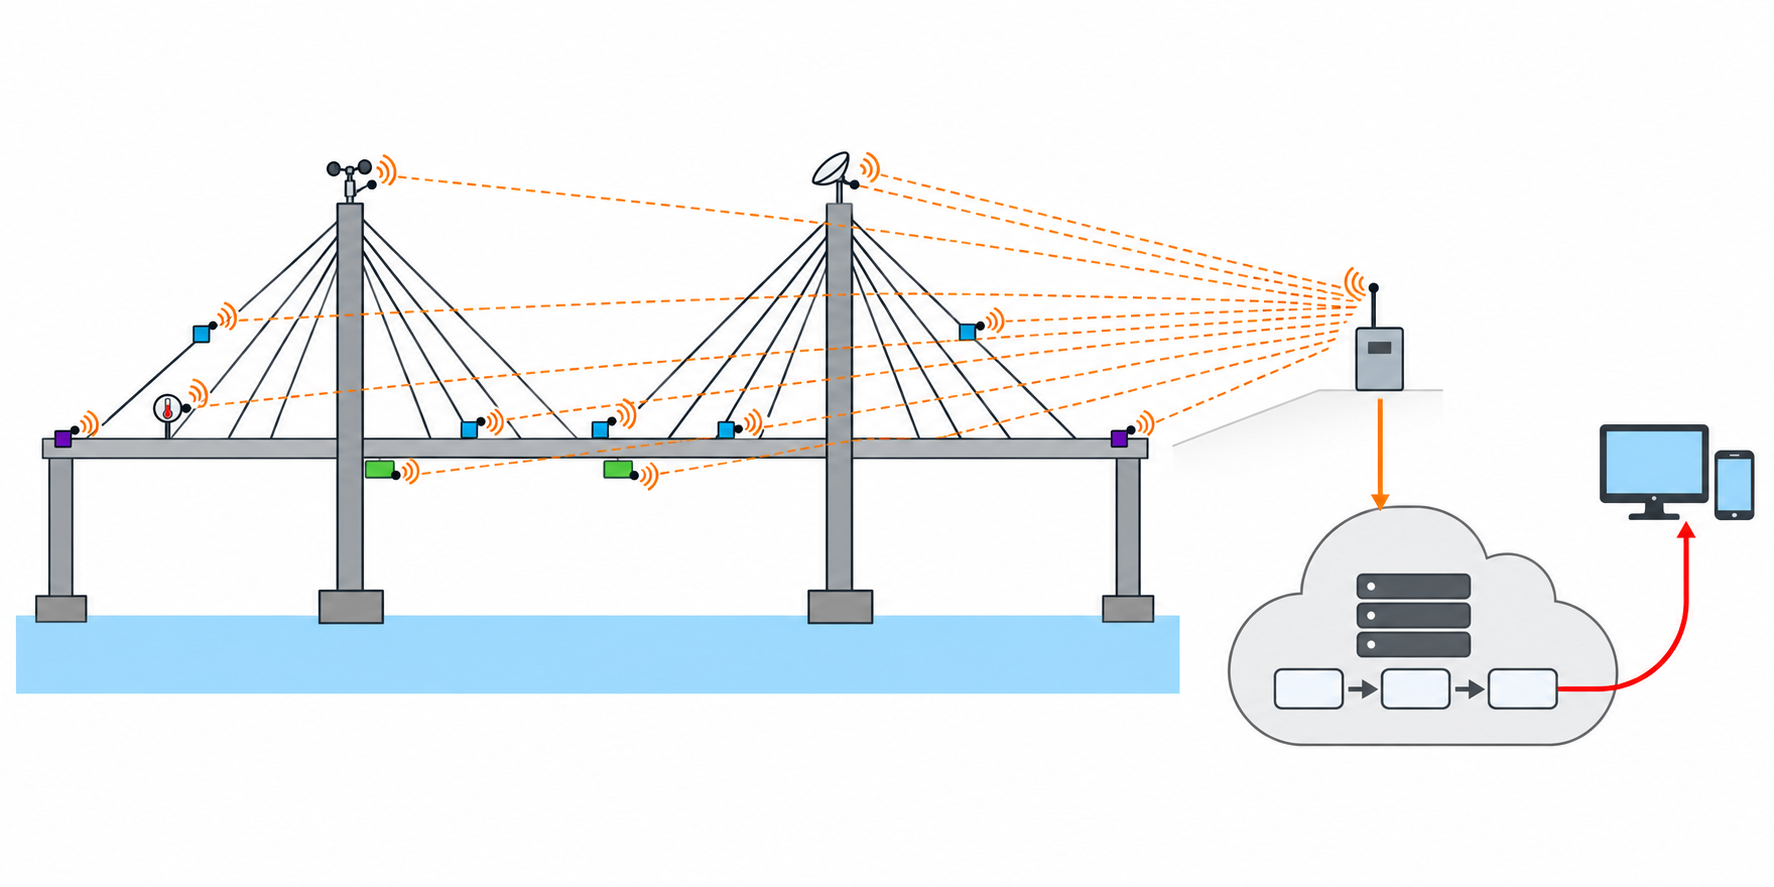
\includegraphics[width=\linewidth]{figures/ch11/ch11-03-v2-brief.png}
\caption{Candidate structural baseline V2 generated from the full brief (second generation run). The twin-pylon bridge form, 16 stay-cable trajectories, 12 sensors, right-hand subsystems, and semantic arrow directions match Table~\ref{tab:ch11-02} with zero baked-in text, serving as the reference baseline for all later versions. However, several reading and consistency flaws remain: the orange wireless dashes are thin, the cloud sits below the gateway, the thermometer icon contains red fill, sensor icons are slightly undersized, and narrow white gaps appear where stay cables pass behind icons (see Table~\ref{tab:ch11-03}). Base art generated by an image model.}\label{fig:ch11-03}
\end{figure}

V2 is a comparison baseline rather than an accepted final figure. Auditing Figure~\ref{fig:ch11-03} against our brief yields the structured \textbf{revision sheet} in Table~\ref{tab:ch11-03}, where every item records its ID, level, location, observed phenomenon, revision requirement, \textbf{what must remain unchanged}, and execution channel.

\begin{table}[htbp]\centering\scriptsize
\setlength{\tabcolsep}{3pt}
\renewcommand{\arraystretch}{1.08}
\caption{Revision sheet compiled from the audit of candidate baseline V2 (Figure~\ref{fig:ch11-03}).}\label{tab:ch11-03}
\begin{tabularx}{\linewidth}{@{}c>{\raggedright\arraybackslash}p{14mm}>{\raggedright\arraybackslash}p{18mm}YYY>{\raggedright\arraybackslash}p{18mm}@{}}
\toprule
\textbf{ID} & \textbf{Level} & \textbf{Location} & \textbf{Observed phenomenon \& impact} & \textbf{Revision requirement} & \textbf{Must remain unchanged} & \textbf{Channel} \\
\midrule
R2 & Reading obstacle & Sensor-to-gateway lines & Orange wireless dashes are thin and lose contrast across stay-cable fans & Change to thicker orange short-dashed lines with wave marks, distinct from dark-gray stay cables & Bridge form, 16 stay cables, 12 sensors, gateway, cloud, terminal, and L2--L4 & Image model (reference edit); TikZ if 2 runs fail \\
R3 & Reading obstacle & All 12 sensors & Blue squares measure $\sim 1.44\text{--}1.80\ \text{mm}$ at $160\ \text{mm}$ width ($<2\ \text{mm}$) & Enlarge sensor icons by $\sim 1.5\times$ (executed separately from R2) & All bridge components, cables, and links as above & Image model (separate round) or vector overlay \\
R4 & Reading obstacle & Right data path & Gateway sits high ($y\approx 0.41$) and cloud sits low ($y\approx 0.71$); upload arrow points down & Adapt label coordinates to actual layout for demo; swap gateway/cloud vertically before submission & Left $70\%$ bridge, 16 stay cables, and 12 sensors & Layout layer adaptation or right-zone redraw \\
V1 & Visual consistency & Thermometer \& blue squares & Thermometer has red fill (violating single-use alert red); blue hex values unverified & Recolor thermometer interior to gray; unify accelerometer blues (e.g., \texttt{\#4C78A8}) & Other sensor icons, structural grays, and red alert arrow & Post-process in vector / image editor \\
V2 & Visual consistency & Cable crossings \& water & Narrow white halo gaps interrupt cables behind icons/waves; mild gradients on water/screen & Bridge cable gaps and flatten gradients in vector or raster editor before submission & Endpoints of all 16 stay cables and sensor positions & Layout layer / vector editor \\
T1 & Labels \& legend & Full canvas \& bottom & Base art has no text; needs component names, subsystem labels, and legend & Overlay 7 labels and a bottom legend in LaTeX/TikZ at measured coordinates & Base bitmap pixels untouched & Layout layer (TikZ) \\
\bottomrule
\end{tabularx}
\end{table}

\begin{BookNote}
\textbf{Three rules for writing a revision sheet:} (1) \textbf{Change only one class of issue at a time}---never bundle thicker dashed lines, larger sensor icons, and a gateway--cloud position swap into a single prompt; (2) \textbf{State an explicit ``must remain unchanged'' inventory}, replacing vague phrases like ``keep everything else the same'' with exact object names and counts; and (3) \textbf{Handle typography, exact color values, gap repairs, and alignment in the layout layer} rather than gambling on repeated generative redraws.
\end{BookNote}

\section{Collateral Changes from Local Edits: How to Spot Them}

Why does Table~\ref{tab:ch11-03} restrict generative edits so tightly? Because a ``local edit'' in a generative image model is not a localized operation on an isolated vector path. When you select a prior image in \scidraw{} (\sdtool{ai-drawing}) as a reference image and submit a modification prompt, the model conditions on both the reference bitmap and your text instruction to \textbf{resynthesize the entire canvas}. There is no ``object locking'' or ``regional pixel freeze'' in generative image editing; as the model redraws the targeted feature, it can silently alter, shift, or drop unmentioned objects---causing \textbf{collateral changes}.

\subsection{Real Case 1: A Style Revision in Chapter 7 Altered Five Structural Features}

Consider first the real iteration record from Chapter 7's mechanism schematic of insulin-stimulated GLUT4 translocation (Figure~\ref{fig:ch11-07}). Its V2 baseline (Figure~\ref{fig:ch11-07}, left) had already verified all 13 signaling objects, 6 amber phosphorylation dots, and five arrow styles. For V3, the author requested only Level 3 stylistic cleanup---unifying protein blue hues, standardizing line weights, and adding whitespace---while specifying ``keep the exact same content and layout.''

When the first V3 run was submitted without attaching the V2 bitmap as a reference image (Figure~\ref{fig:ch11-07}, middle), the colors and strokes became cleaner, but five severe structural collateral changes appeared simultaneously: (a) all six phosphorylation dots on the receptor, IRS-1, Akt, and AS160 vanished; (b) insulin dropped from three beads to two and detached from the receptor; (c) PDK1 and Akt detached from the inner leaflet of the plasma membrane into the cytosol; (d) an unrequested solid activation arrow appeared between PI3K and PDK1; and (e) each storage vesicle acquired multiple GLUT4 barrels instead of one, alongside stray intracellular glucose hexagons. Only in the second run, when V2 was passed as a reference image (Figure~\ref{fig:ch11-07}, right), were the main structure and phosphorylation dots preserved. Even with a reference image attached, Chapter 7's palette counter-example experiment showed the model quietly turning the open arrowhead on the $\text{PIP}_2 \rightarrow \text{PIP}_3$ conversion arc into a filled arrowhead.

\begin{figure}[htbp]\centering
% FIG ch11-07 Chapter 7 collateral reuse (English)
\usetikzlibrary{arrows.meta,calc}
\begin{tikzpicture}
  \def\panelW{0.31\linewidth}
  \definecolor{Ch11AnnotRed}{HTML}{C0392B}
  \node[anchor=south west, inner sep=0] (imA) at (0,0) {%
    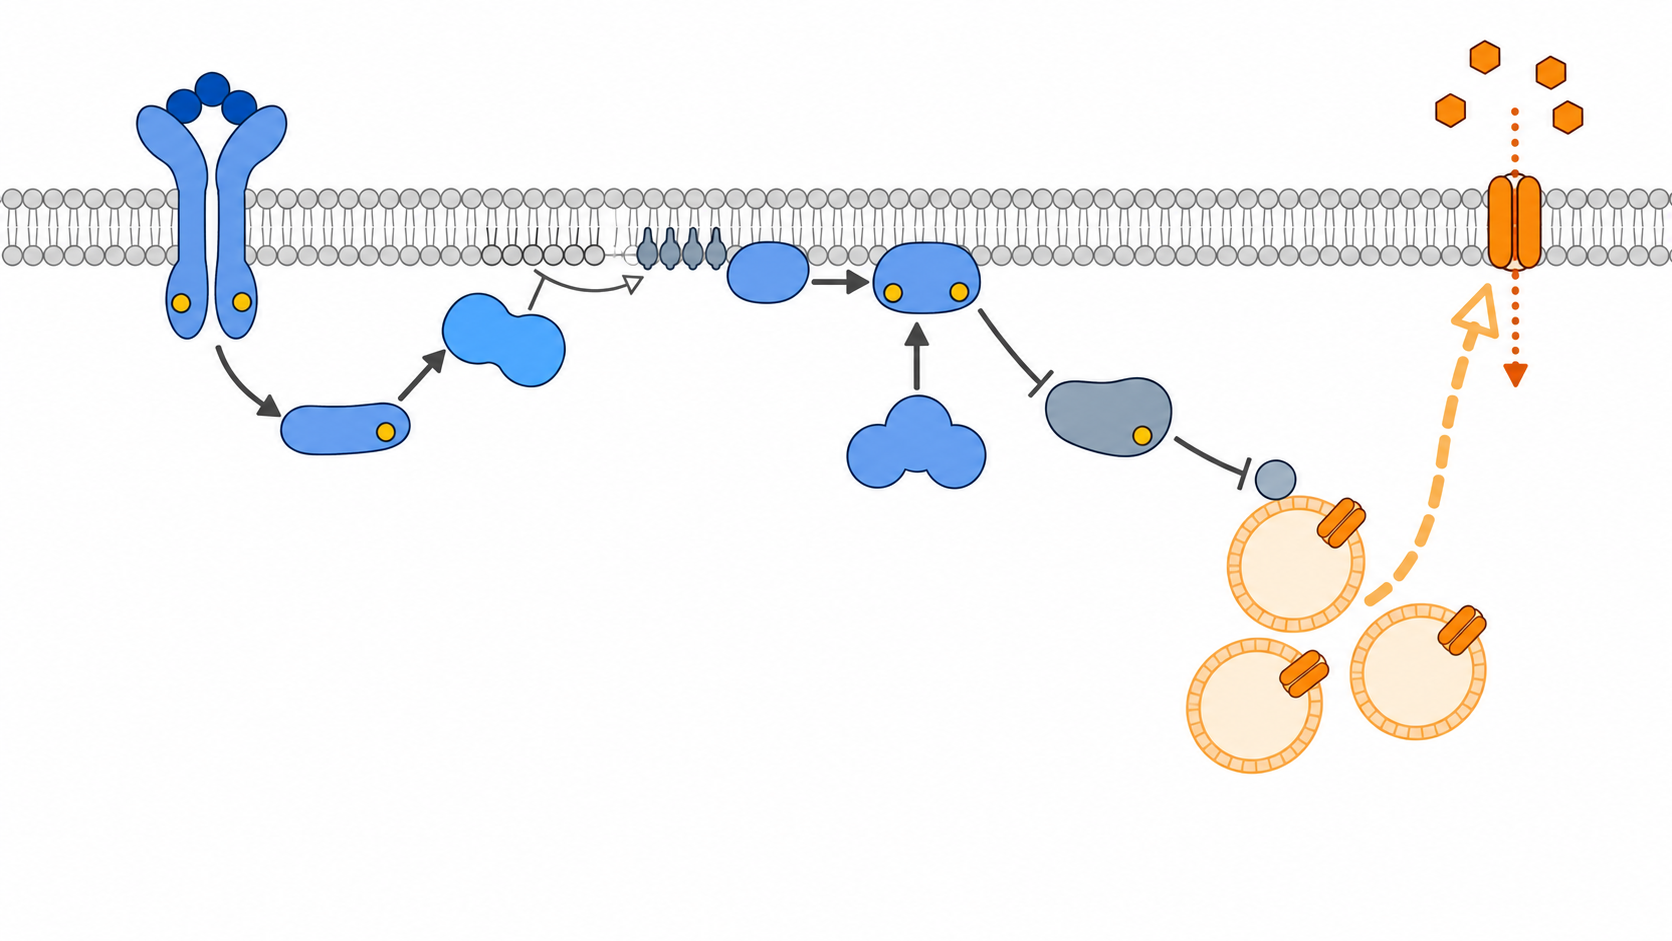
\includegraphics[width=\panelW]{figures/ch11/ch11-07a-ch07-v2.png}};
  \node[font=\small\sffamily, anchor=south] at ($(imA.north)+(0,2mm)$) {V2 baseline};

  \node[anchor=south west, inner sep=0] (imB) at (0.345\linewidth,0) {%
    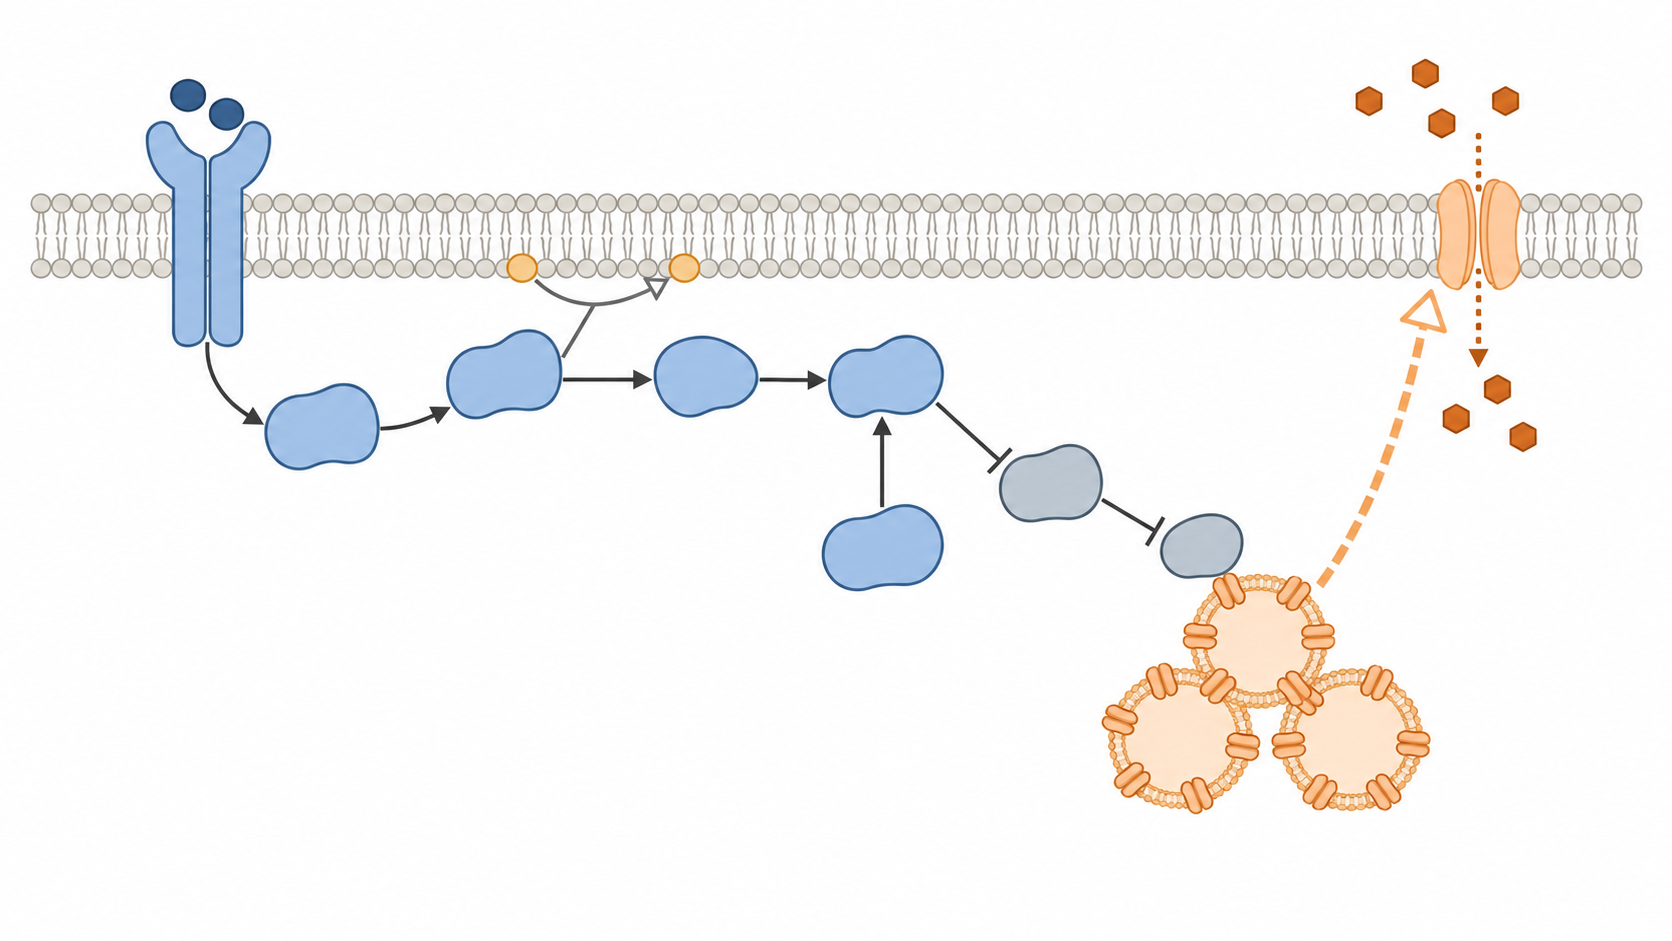
\includegraphics[width=\panelW]{figures/ch11/ch11-07b-ch07-v3-alt1.png}};
  \node[font=\small\sffamily, anchor=south] at ($(imB.north)+(0,2mm)$) {V3, attempt 1 (rejected)};
  \begin{scope}[x={(imB.south east)},y={(imB.north west)}]
    \draw[Ch11AnnotRed, line width=0.7pt] (0.11,0.28) circle (0.035);
    \node[font=\scriptsize\sffamily, text=Ch11AnnotRed, anchor=west] at (0.15,0.28) {(a)};
    \draw[Ch11AnnotRed, line width=0.7pt] (0.10,0.08) circle (0.04);
    \node[font=\scriptsize\sffamily, text=Ch11AnnotRed, anchor=west] at (0.14,0.08) {(b)};
    \draw[Ch11AnnotRed, line width=0.7pt] (0.48,0.38) circle (0.06);
    \node[font=\scriptsize\sffamily, text=Ch11AnnotRed, anchor=west] at (0.54,0.38) {(c)};
    \draw[Ch11AnnotRed, line width=0.7pt] (0.34,0.36) circle (0.045);
    \node[font=\scriptsize\sffamily, text=Ch11AnnotRed, anchor=west] at (0.39,0.36) {(d)};
    \draw[Ch11AnnotRed, line width=0.7pt] (0.76,0.70) circle (0.07);
    \node[font=\scriptsize\sffamily, text=Ch11AnnotRed, anchor=west] at (0.82,0.70) {(e)};
  \end{scope}

  \node[anchor=south west, inner sep=0] (imC) at (0.69\linewidth,0) {%
    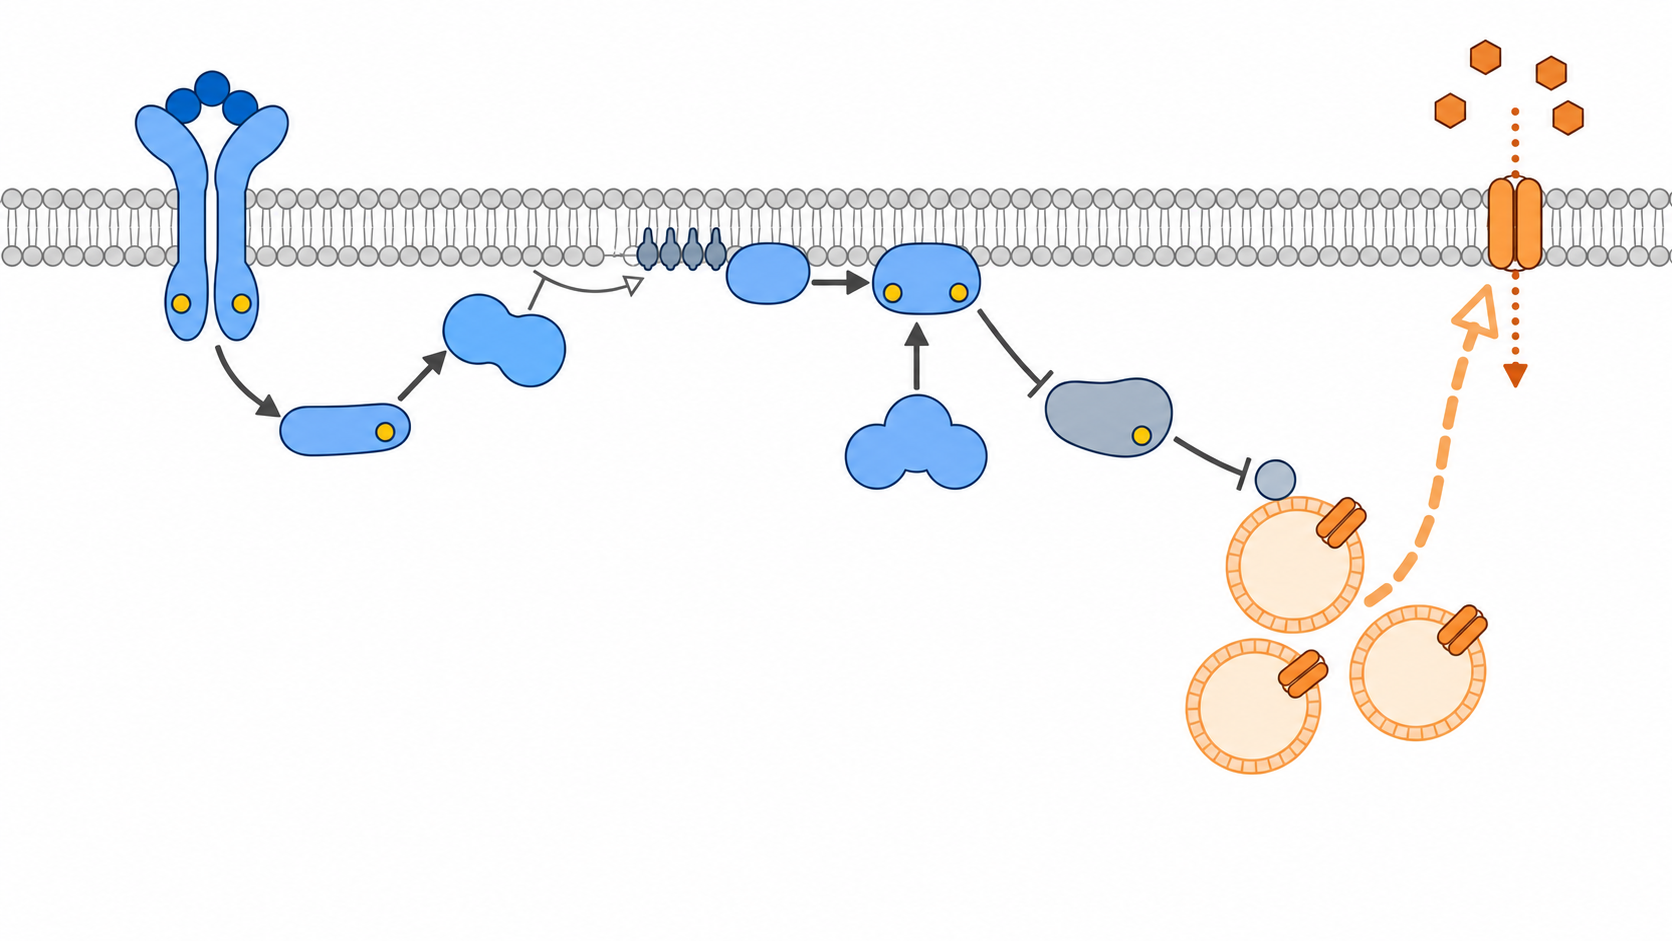
\includegraphics[width=\panelW]{figures/ch11/ch11-07c-ch07-v3.png}};
  \node[font=\small\sffamily, anchor=south] at ($(imC.north)+(0,2mm)$) {V3, attempt 2 (accepted)};
\end{tikzpicture}

\caption{A real iteration from Chapter 7: an instruction about colour and line style can still change the structure. Left, V2 baseline. Middle, V3 attempt 1 (generated from the revised prompt without a reference image): (a) all phosphorylation marks lost; (b) insulin reduced from three beads to two and detached from the receptor; (c) PDK1 and Akt moved off the membrane; (d) an unrequested PI3K$\rightarrow$PDK1 activation arrow added; (e) several GLUT4 per vesicle instead of one. Right, attempt 2 of the same instruction with V2 passed as a reference image keeps the main structure but still needs a full check. All three generated by an image model.}\label{fig:ch11-07}
\end{figure}

\subsection{Real Case 2: Three Reference-Image Revision Runs for V3 in This Chapter}

Now examine item R2 on our revision sheet. Inside \scidraw{} (\sdtool{ai-drawing}), we select V2 (Figure~\ref{fig:ch11-03}) from the history as our reference image and formulate a single-issue instruction targeting only the wireless links:

\begin{Prompt}
Target edit (Item R2): Change only the wireless transmission lines from the sensors
to the gateway into thicker orange short-dashed lines with small wave marks so they
are immediately distinguishable from the stay cables. Keep everything else unchanged.
\end{Prompt}

The exact English prompt submitted with V2 attached as the reference image was:

\begin{Prompt}
Using the reference image, change only the wireless lines from the sensors to
the gateway: make them thicker orange short-dashed lines with small wave marks,
so they cannot be confused with the stay cables. Keep everything else
unchanged. No text.
\end{Prompt}

We executed three independent reference-image edits from V2, auditing all objects against Table~\ref{tab:ch11-02} each time. Figure~\ref{fig:ch11-04} compares V2 (left) with V3 attempt 1 (right).

\begin{figure}[htbp]\centering
\resizebox{\linewidth}{!}{%
\begin{tikzpicture}
\definecolor{Ch11OkGreen}{HTML}{2E8B57}
\definecolor{Ch11WarnRed}{HTML}{C0392B}
\node[anchor=south west,inner sep=0] (imL) at (0,0) {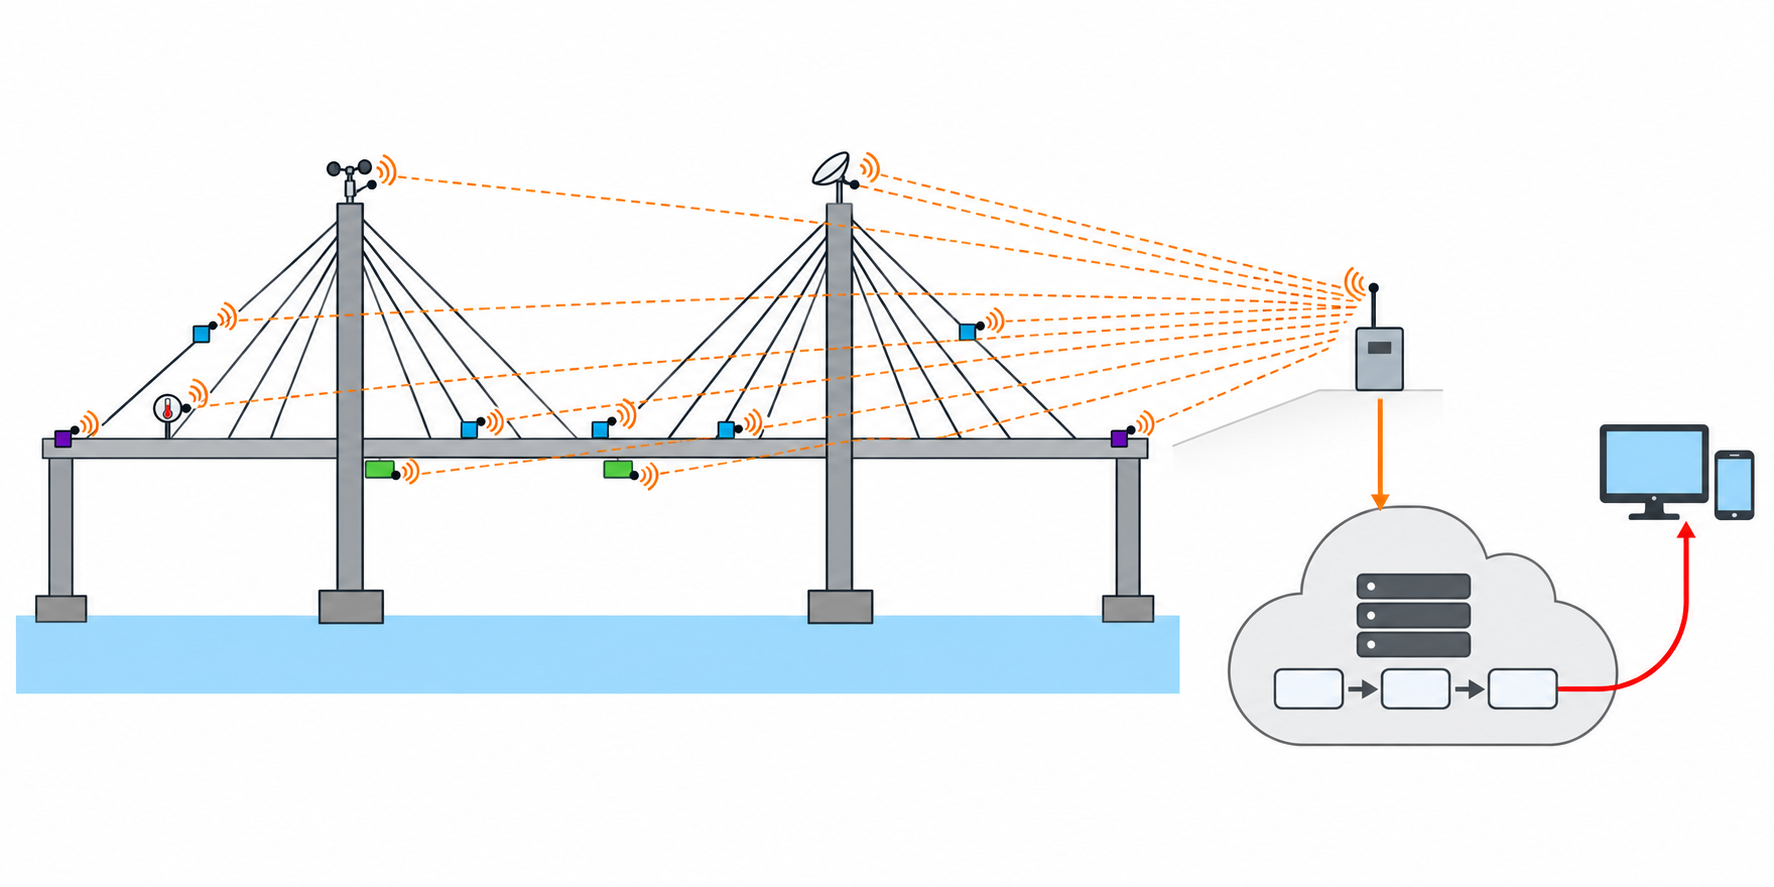
\includegraphics[width=0.488\linewidth]{figures/ch11/ch11-03-v2-brief.png}};
\node[font=\sffamily\footnotesize,anchor=south] at ($(imL.north)+(0,1.5mm)$) {V2 candidate baseline (before edit)};
\node[anchor=south west,inner sep=0] (imR) at (0.512\linewidth,0) {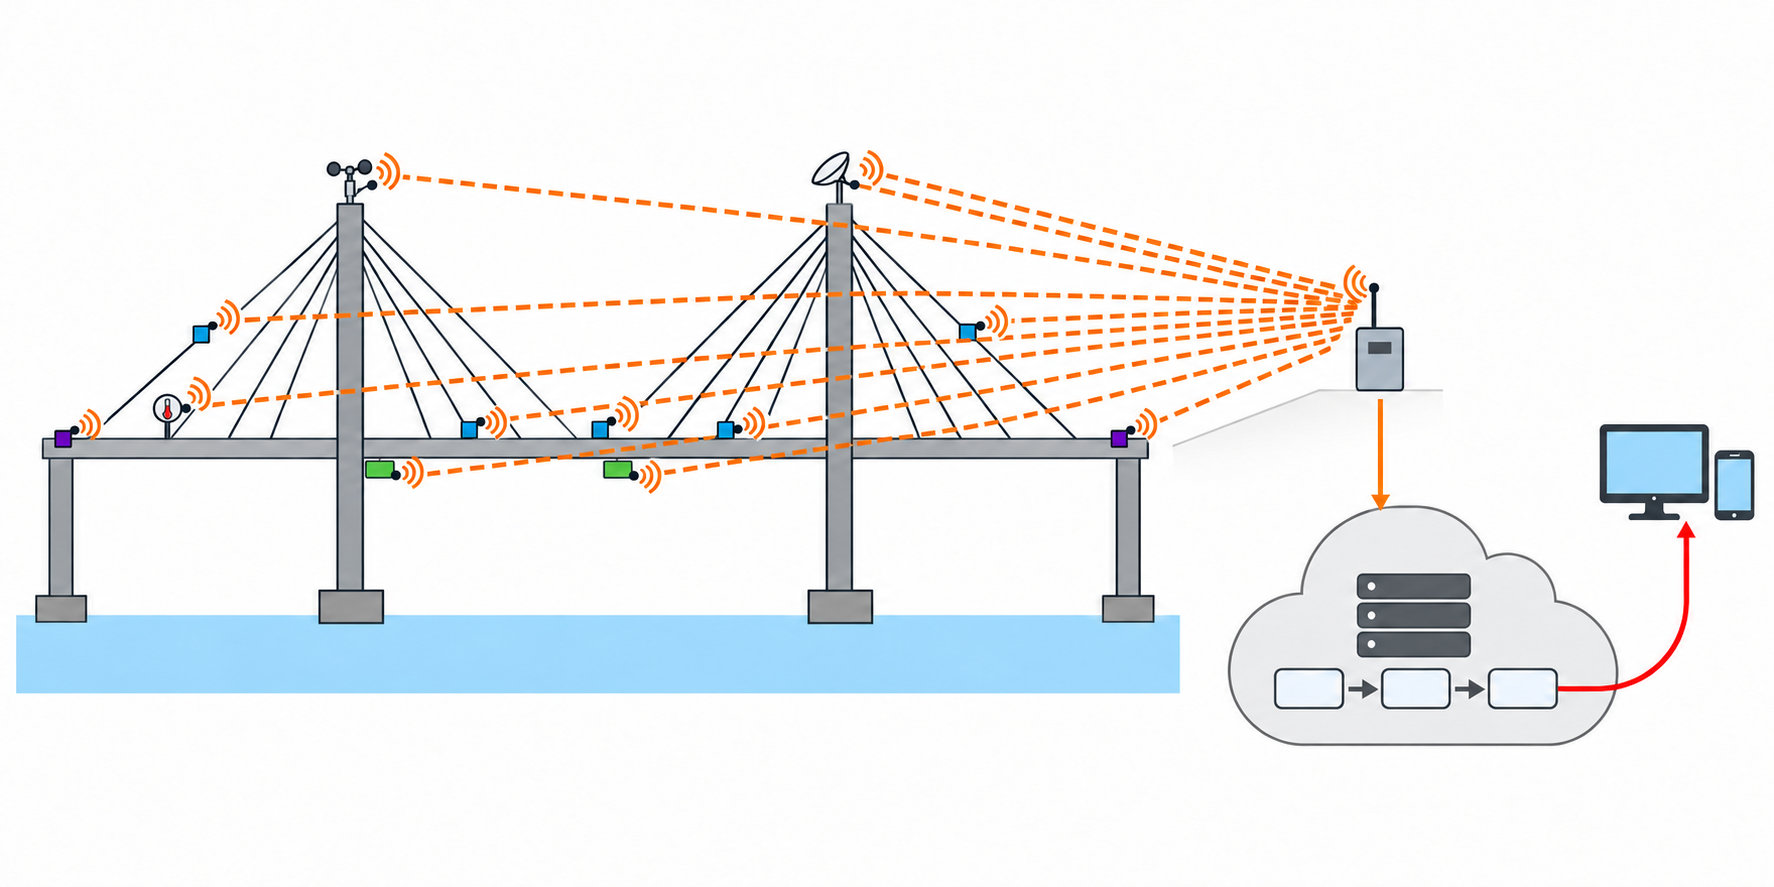
\includegraphics[width=0.488\linewidth]{figures/ch11/ch11-04-v3-collateral.png}};
\node[font=\sffamily\footnotesize,anchor=south] at ($(imR.north)+(0,1.5mm)$) {V3, attempt 1 (after reference-image edit)};
\begin{scope}[x={(imR.south east)},y={(imR.north west)}]
  \draw[Ch11OkGreen,line width=0.9pt,rounded corners=2pt] (0.50,0.61) rectangle (0.76,0.80);
  \node[fill=white,fill opacity=0.9,text opacity=1,text=Ch11OkGreen,font=\sffamily\bfseries\scriptsize,inner sep=1pt,anchor=south] at (0.63,0.81) {Target edit done: thicker orange dashes};
  \draw[Ch11WarnRed,dashed,line width=0.7pt,rounded corners=2pt] (0.06,0.49) rectangle (0.13,0.59);
  \node[fill=white,fill opacity=0.9,text opacity=1,text=Ch11WarnRed,font=\sffamily\scriptsize,inner sep=1pt,anchor=south] at (0.10,0.60) {Inherited flaw 1};
  \draw[Ch11WarnRed,dashed,line width=0.7pt,rounded corners=2pt] (0.68,0.14) rectangle (0.91,0.44);
  \node[fill=white,fill opacity=0.9,text opacity=1,text=Ch11WarnRed,font=\sffamily\scriptsize,inner sep=1pt,anchor=north] at (0.80,0.13) {Inherited flaw 2: cloud below gateway};
\end{scope}
\end{tikzpicture}}
\caption{V3 attempt 1 (right), produced by asking only for a change to the wireless lines, beside the candidate baseline V2 (left). The solid green box marks the completed target edit (thicker orange short-dashed lines and clearer wave marks near sensor nodes). Across three independent reference-image edits, all 16 stay-cable trajectories and 12 sensors were preserved without observable structural collateral changes, though a full-figure check was required to confirm this. Dashed red boxes mark pre-existing baseline flaws inherited unchanged from V2 (red fill inside the thermometer and the cloud positioned below the gateway). Base art generated by an image model without manual alteration.}\label{fig:ch11-04}
\end{figure}

The three empirical runs establish three points: (1) \textbf{Target edit completed:} all three runs thickened the orange short-dashed lines and made the wave marks near the sensor nodes more prominent, clearly distinguishing radio links from the thin dark-gray stay cables (though waves stayed near the nodes rather than along mid-span segments); (2) \textbf{No structural collateral changes observed across all three runs:} 2 pylons, 16 stay-cable trajectories ($4+4+4+4$), 12 sensors ($3+2+2+1+1+1+2$), the gateway, cloud, 3 processing boxes, terminal, and arrows L2--L4 remained consistent with V2; and (3) \textbf{Pre-existing V2 flaws were inherited unchanged:} the red thermometer interior (Inherited flaw 1), the cloud below the gateway (Inherited flaw 2), small sensor icons, and narrow white cable gaps persisted in all three outputs.

This demonstrates the stochastic nature of generative edits: \textbf{``no collateral change occurred this time'' is a conclusion you can state only after a full item-by-item count, never an assumption you can make beforehand.}

\subsection{Verifying with Side-by-Side Comparison, Pixel Difference Maps, and Object Count Tables}

Catching collateral changes relies on combining three complementary methods (Figure~\ref{fig:ch11-05}):

\begin{figure}[htbp]\centering
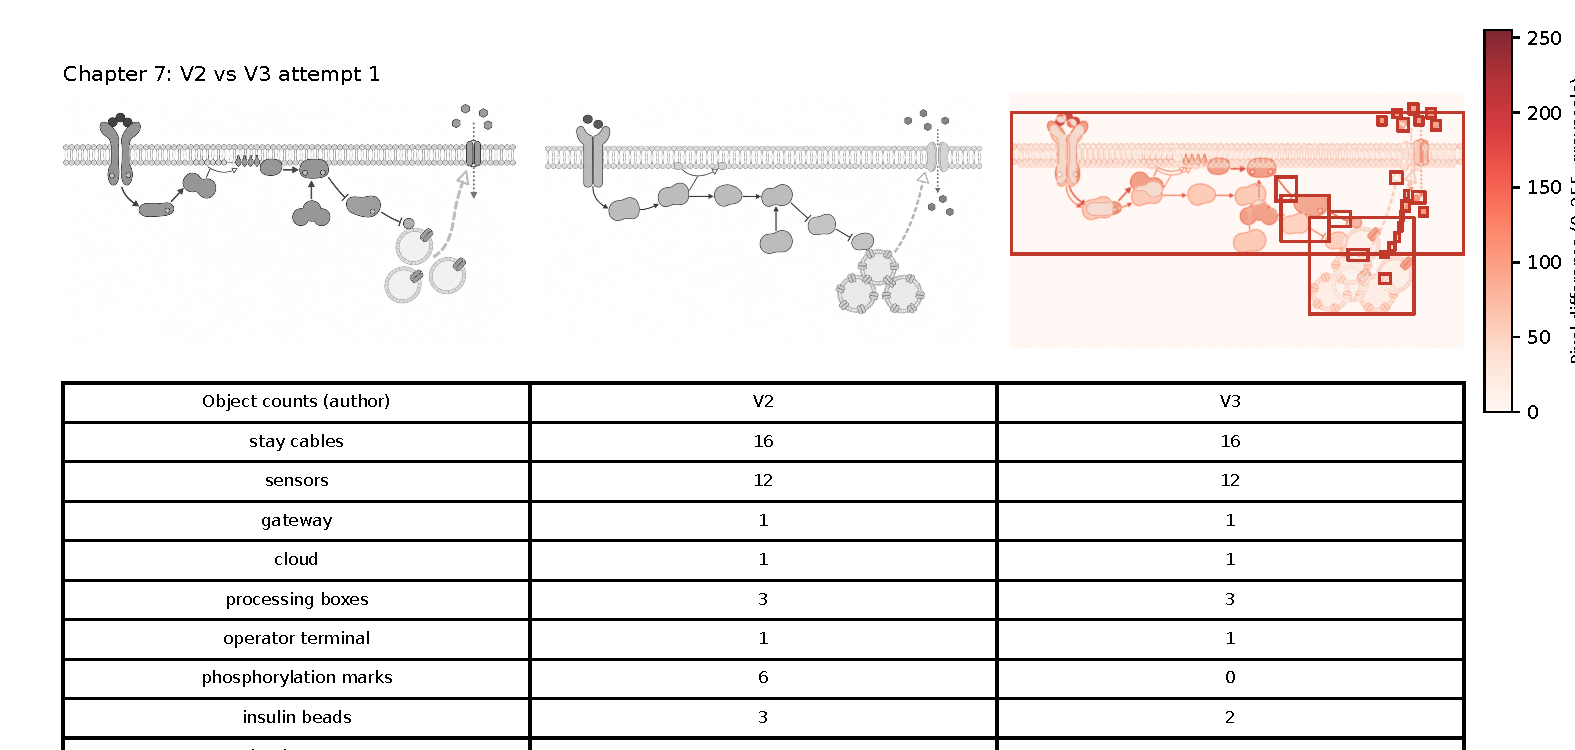
\includegraphics[width=\linewidth]{figures/ch11/ch11-05-diff-and-count-en.pdf}
\caption{Finding collateral changes with a difference map and an object count. The difference map shows where grayscale pixels changed between two versions. When the layout is preserved it points straight at altered or missing objects; when the whole image is redrawn and repositioned (top row: Chapter 7's V2 and the first V3 attempt), difference bounding boxes cover everything (24 regions across $14.6\%$ of pixels) and only an object-by-object count still works (bottom table: first 6 rows for this chapter's V2 vs.\ V3; last 4 rows for Chapter 7). Counts were made by the author.}\label{fig:ch11-05}
\end{figure}

First, \textbf{same-scale side-by-side comparison or rapid blink toggling}. Because \scidraw{} does not currently include an in-app side-by-side comparator, download the old and new versions and align them at equal width (as in Figure~\ref{fig:ch11-04}), or flip rapidly between them in an image viewer so any displaced or missing element flickers into view.

Second, \textbf{pixel difference heatmaps and their limitation}. After scaling two versions to equal dimensions and converting them to grayscale ($0\text{--}255$), you compute the absolute pixel difference, apply a Gaussian blur (radius $\approx 2\ \text{px}$) to suppress anti-aliasing noise, and box connected regions exceeding a difference of $40$. When background coordinates stay fixed, the heatmap pinpoints altered lines; when the model rearranges the layout globally---as in Chapter 7's V2 versus V3 attempt 1 (top row of Figure~\ref{fig:ch11-05})---$14.6\%$ of pixels exceed the threshold and 24 red boxes blanket the canvas, losing localization power.

Third, \textbf{the manual object count table (the final line of defense)}. Counting entities row by row against the inventory table (bottom of Figure~\ref{fig:ch11-05}) confirms that our bridge V2 and V3 match across stay cables ($16/16$), sensors ($12/12$), gateway ($1/1$), cloud ($1/1$), processing boxes ($3/3$), and terminal ($1/1$). In contrast, Chapter 7's V2 versus V3 attempt 1 drops phosphorylation dots from $6$ to $0$ and insulin beads from $3$ to $2$, while increasing activation arrows from $4$ to $5$ and maximum GLUT4 per vesicle from $1$ to $3$. Difference maps assist the eye, but manual table counts safeguard the science.

\section{Branching Back to the Previous Version, and When to Move to the Layout Layer}

Once an audit uncovers a collateral change (such as a missing antenna or lost stay cable), never stay on the broken V3 and prompt ``add the missing antenna back.'' As the dashed box at the lower right of Figure~\ref{fig:ch11-08} illustrates, stacking patches onto a defective version ($\text{V3} \rightarrow \text{V3}' \rightarrow \text{V3}''$) causes each full-canvas redraw to introduce fresh drift, compounding errors until their origin is untraceable.

\begin{figure}[htbp]\centering
\resizebox{\linewidth}{!}{\tikzset{every node/.append style={align=center}}% FIG ch11-08 version tree (English)
\usetikzlibrary{arrows.meta,positioning,fit,calc}
\definecolor{Ch11BadRed}{HTML}{C0392B}
\definecolor{Ch11GoodGreen}{HTML}{2E8B57}
\providecommand{\ChElevenThumb}[2]{%
  \IfFileExists{#1}{%
    \includegraphics[width=24mm]{#1}%
  }{%
    \fbox{\parbox[c][16mm][c]{24mm}{\centering\scriptsize\sffamily #2\\{\tiny (base pending)}}}}%
}
\begin{tikzpicture}[
  x=1mm, y=1mm,
  font=\sffamily\footnotesize,
  edge/.style={draw=BookInk!60, -{Stealth[length=2mm]}, line width=0.55pt},
  badedge/.style={draw=Ch11BadRed!70, dashed, -{Stealth[length=2mm]}},
  nlabel/.style={align=center, text width=26mm, font=\scriptsize},
]
  \node (V1) at (0,0) {\ChElevenThumb{figures/ch11/ch11-02-v1-vague.png}{V1}};
  \node[nlabel, below=1mm of V1] {One-line prompt};

  \node (V2) [below=14mm of V1] {\ChElevenThumb{figures/ch11/ch11-03-v2-brief.png}{V2\\baseline}};
  \node[nlabel, below=1mm of V2] {\textbf{Structural baseline}};

  \node (V3) [below=14mm of V2] {\ChElevenThumb{figures/ch11/ch11-04-v3-collateral.png}{V3}};
  \node[nlabel, below=1mm of V3, text=Ch11BadRed] {Collateral change\\{\tiny (rejected)}};

  \node (V4) at (42,-28) {\ChElevenThumb{figures/ch11/ch11-06-v4-recovered.png}{V4}};
  \node[nlabel, below=1mm of V4, text=Ch11GoodGreen] {Back to V2\\wireless lines only};

  \node (Final) at (84,-28) {\ChElevenThumb{figures/ch11/ch11-06-v4-recovered.png}{Final}};
  \node[nlabel, below=1mm of Final] {TikZ labels \& legend};

  \draw[edge] (V1) -- node[left, font=\tiny, align=right] {Rewrite\\input} (V2);
  \draw[edge] (V2) -- node[right=1.5mm, font=\tiny, align=left] {Wireless\\lines only} (V3);
  \draw[edge] (V2.east) -- node[above, font=\tiny] {Wireless +\\keep list} (V4.west);
  \draw[edge] (V4.east) -- node[above, font=\tiny] {Labels \&\\legend} (Final.west);

  \node[draw=Ch11BadRed, dashed, rounded corners=2pt, inner sep=4pt, fit=(V3)] {};
  \node[font=\scriptsize, text=Ch11BadRed, right=1mm of V3] {×};

  \node (Vp1) at (42,-66) {\fbox{\parbox[c][16mm][c]{24mm}{\centering\scriptsize V3$'$\\schematic}}};
  \node[font=\tiny, below=1mm of Vp1, text width=28mm, align=center] {Add back missing antenna};
  \node (Vp2) [right=12mm of Vp1] {\fbox{\parbox[c][16mm][c]{24mm}{\centering\scriptsize V3$''$\\schematic}}};
  \node[font=\tiny, below=1mm of Vp2, text width=28mm, align=center] {Another drift};
  \draw[badedge] (Vp1) -- (Vp2);
  \node[draw=BookInk!40, dashed, rounded corners=2pt, inner sep=6pt,
    fit=(Vp1)(Vp2), label={[font=\scriptsize, yshift=2mm]above:Wrong: patch the faulty version}] {};
  \draw[badedge] (V3.east) -- ++(6,0) |- (Vp1.west);
\end{tikzpicture}
}
\caption{Version tree for this chapter's case. When a revision shows collateral changes, do not patch the faulty version; return to the V2 baseline and branch again (V4), restating what must stay and changing one thing. The dashed box shows how patching a faulty version piles up problems that are hard to trace. (Note: our three V3 runs did not lose structural objects; the V3 branch here illustrates the standard rollback logic when collateral changes occur.)}\label{fig:ch11-08}
\end{figure}

Instead, \textbf{re-select the baseline V2 from your \scidraw{} history} to start a clean branch (V4), pairing your single modification request with an item-by-item preservation checklist:

\begin{Prompt}
Use this reference image as the basis for the edit. Change only one thing:
make the wireless transmission lines from the sensors to the gateway thicker
orange short-dashed lines with small wave marks.
The following must remain unchanged, item by item:
- The side view of the twin-pylon cable-stayed bridge; the positions, heights
  and shapes of both pylons.
- All 16 stay cables: 4 on the left and 4 on the right of each pylon, all
  connecting a pylon to the deck; their positions and angles.
- The positions, shapes and colors of all 12 sensors: 3 blue squares on the
  main-span deck; 1 blue square at the middle of each of the two longest
  outer cables; 2 green rectangles under the deck; the anemometer on top of
  the left pylon; the GNSS antenna on top of the right pylon; the thermometer
  on the left side span; and 2 purple squares at the deck ends.
- The positions of the gateway, cloud, 3 processing boxes inside the cloud,
  and operator terminal; the orange upload arrow and the red alert arrow.
- Do not add any new objects, new lines or text.
If you cannot make the edit without changing anything else, leave the
original image unchanged.
\end{Prompt}

Executing this prompt with V2 as the reference image produced the V4 base image: the orange short-dashed wireless links were thickened, all 16 stay-cable trajectories and 12 sensors were preserved, and grayscale conversion confirmed clear separation between the thick dashed wireless links and thin solid stay cables.

If a local modification still causes collateral changes twice in a row despite an explicit preservation checklist, \textbf{switch to the layout-layer route}: replace the wireless-line clause in the V2 prompt with \texttt{Do not draw any lines from sensors to the gateway}, generate a link-free base image, verify all 16 stay cables and 12 sensors, and draw the orange dashed links and wave marks in TikZ (the cost is re-auditing the new base image once; the benefit is that future line-style edits never touch the bitmap).

By contrast, data charts in \scidraw{} Scientific Visualization (\sdtool{sci-vis}) are redrawn from code or chart configurations and support conversational edits plus one-click restoration to the previous or original version without randomly dropping data points. Nevertheless, data plots still require full-figure re-verification after every edit or rollback to ensure that updated axis limits did not clip extreme values or distort statistical comparisons.

\section{Revision Logs, Overlaid Final Figure, and Full-Figure Re-Verification}

Every iteration should leave a row in your revision log recording the parent version, prompt summary, target edit, observed deviations or collateral changes, and adoption decision (Table~\ref{tab:ch11-04}).

\begin{table}[htbp]\centering\scriptsize
\setlength{\tabcolsep}{3pt}
\renewcommand{\arraystretch}{1.08}
\caption{Version-by-version revision log for the cable-stayed bridge SHM schematic case study.}\label{tab:ch11-04}
\begin{tabularx}{\linewidth}{@{}l>{\raggedright\arraybackslash}p{13mm}>{\raggedright\arraybackslash}p{21mm}YY>{\raggedright\arraybackslash}p{18mm}@{}}
\toprule
\textbf{Version} & \textbf{Based on} & \textbf{Prompt summary} & \textbf{Target change \& positive results} & \textbf{Observed deviations or collateral changes} & \textbf{Decision} \\
\midrule
V1 (1 run) & --- & One-line vague English prompt & Produced photorealistic counter-example & 6 scientific errors S1--S6 (6-pylon 3D bridge, missing anemometer/GNSS, bidirectional arrow, fabricated waveforms, ``92\%'' score, dated alarms) & Rejected; rewrite input \\
V2, run 1 & Brief & Full structured English prompt & Twin-pylon side view, 12 sensors, zero text & $200\%$ check showed only 12 stay cables reaching pylons ($3+3+3+3$) plus 1 floating diagonal segment on left & Rejected (archived alt1) \\
V2, run 2 & Brief & Same full prompt, 2nd run & 16 stay-cable trajectories, 12 sensors, subsystems, and 4 arrow directions correct; zero text & Wireless dashes thin; cloud below gateway; red inside thermometer; small sensor icons; narrow white gaps where cables cross icons & Selected as baseline V2 \\
V2, run 3 & Brief & Same full prompt, 3rd run & 16 stay-cable trajectories and 12 sensors countable & Main-span cables cross in a crowded tangle; anemometer colored blue; gateway floats; cloud presses into water band & Rejected (archived alt2) \\
V3 (3 runs) & V2 & Reference edit: thicken wireless dashes + waves & All 3 runs thickened orange short dashes and enhanced node wave marks & No missing cables or sensors across 3 runs; inherited V2's low cloud, red thermometer, small icons, and cable gaps & Run 1 shown in Fig.~\ref{fig:ch11-04} \\
V4 (1 run) & V2 & Back to V2 + wireless edit + keep list & Orange wireless dashes thickened; 16 cables and 12 sensors preserved; distinct in grayscale & No new collateral changes; still inherits V2's cloud below gateway, red thermometer, small icons, and narrow cable gaps & Selected as base for overlay \\
Overlaid final & V4 & TikZ callout labels and bottom legend & 7 structural/subsystem labels and two-row legend added at $\ge 6\ \text{pt}$ vector text & Base bitmap unretouched; 4 inherited base deviations documented in Table~\ref{tab:ch11-05} & Teaching demo final \\
\bottomrule
\end{tabularx}
\end{table}

When overlaying labels and a legend onto the V4 base image in TikZ, \textbf{measure coordinates from the actual object positions in the selected bitmap rather than copying planned coordinates from the brief}. Although the brief requested the cloud at upper right and the gateway at lower right, the actual bitmap placed the gateway higher up ($\sim 0.60$ from the bottom) and the cloud lower down (with the three processing boxes centered near $y \approx 0.224$); calibrating coordinates to the actual artwork prevents mislabeling (Figure~\ref{fig:ch11-06}).

\begin{figure}[htbp]\centering
\begin{tikzpicture}
\definecolor{Ch11Blue}{HTML}{2B8CBE}
\definecolor{Ch11Green}{HTML}{4DAF4A}
\definecolor{Ch11Purple}{HTML}{7B3294}
\definecolor{Ch11Orange}{HTML}{E66101}
\definecolor{Ch11Red}{HTML}{C0392B}
\definecolor{Ch11Gray}{HTML}{4A4A4A}
\node[anchor=south west,inner sep=0] (img) at (0,0) {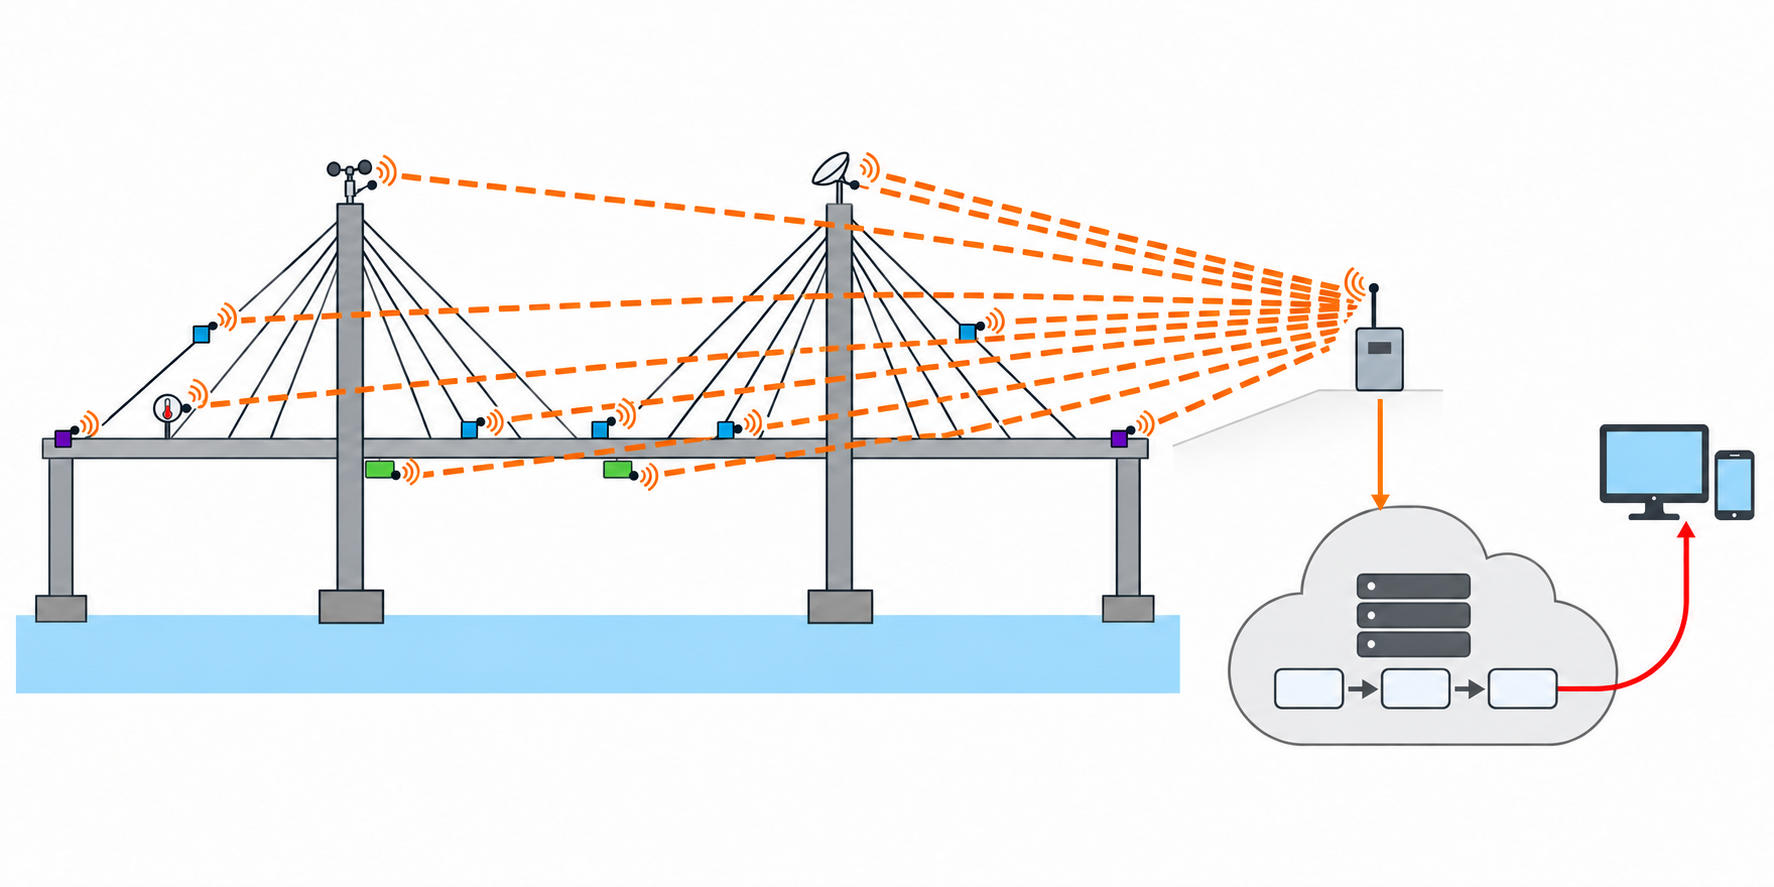
\includegraphics[width=\linewidth]{figures/ch11/ch11-06-v4-recovered.png}};
\begin{scope}[x={(img.south east)},y={(img.north west)}]
  \tikzset{
    lbl/.style={font=\sffamily\scriptsize,text=BookInk,fill=white,fill opacity=0.88,text opacity=1,inner sep=1.2pt,rounded corners=1pt,align=center},
    boxlbl/.style={font=\sffamily\tiny,text=BookInk,align=center,inner sep=0.5pt},
    ldr/.style={draw=BookInk!65,line width=0.45pt}
  }
  \node[lbl] (t1) at (0.11,0.77) {Pylon};
  \draw[ldr] (t1.east) -- (0.19,0.73);
  \node[lbl] (t2) at (0.33,0.76) {Stay cables (16 total)};
  \draw[ldr] (t2.south) -- (0.29,0.66);
  \node[lbl] (t3) at (0.56,0.42) {Deck girder};
  \draw[ldr] (t3.north) -- (0.56,0.49);
  \node[lbl,text=Ch11Orange!90!black] at (0.62,0.80) {Wireless links};
  \node[lbl] (t5) at (0.86,0.64) {On-site gateway};
  \draw[ldr] (t5.west) -- (0.80,0.61);
  \node[lbl] at (0.80,0.45) {Cloud analytics subsystem};
  \node[boxlbl] at (0.738,0.224) {Data\\[-1pt]cleaning};
  \node[boxlbl] at (0.798,0.224) {Feature\\[-1pt]extraction};
  \node[boxlbl] at (0.859,0.224) {Threshold/\\[-1pt]anomaly};
  \node[lbl,text=Ch11Red,anchor=east] (t7) at (0.985,0.58) {Alert to operators\\[-1pt]{\tiny(engineer review)}};
  \draw[draw=Ch11Red,line width=0.45pt] (t7.south) -- (0.94,0.51);

  \draw[draw=BookRule,fill=BookPale!55,rounded corners=2pt,line width=0.4pt] (0.015,0.015) rectangle (0.985,0.115);
  \node[font=\sffamily\bfseries\tiny,text=BookInk,anchor=west] at (0.022,0.082) {Sensors:};
  \filldraw[fill=Ch11Blue,draw=Ch11Gray,line width=0.4pt] (0.105,0.072) rectangle (0.117,0.092);
  \fill[black] (0.121,0.082) circle (0.0025);
  \node[font=\sffamily\tiny,text=BookInk,anchor=west] at (0.126,0.082) {Accelerometer (3 deck / 2 cable)};
  \filldraw[fill=Ch11Green,draw=Ch11Gray,line width=0.4pt] (0.380,0.074) rectangle (0.398,0.090);
  \node[font=\sffamily\tiny,text=BookInk,anchor=west] at (0.403,0.082) {Strain gauge (2)};
  \draw[Ch11Gray,line width=0.5pt] (0.535,0.070) -- (0.535,0.092);
  \draw[Ch11Gray,line width=0.5pt] (0.527,0.088) -- (0.543,0.088);
  \fill[Ch11Gray] (0.527,0.088) circle (0.003);
  \fill[Ch11Gray] (0.543,0.088) circle (0.003);
  \node[font=\sffamily\tiny,text=BookInk,anchor=west] at (0.548,0.082) {Anemometer (1)};
  \draw[Ch11Gray,fill=white,line width=0.5pt] (0.685,0.084) ellipse (0.008 and 0.005);
  \draw[Ch11Gray,line width=0.5pt] (0.685,0.071) -- (0.685,0.080);
  \node[font=\sffamily\tiny,text=BookInk,anchor=west] at (0.697,0.082) {GNSS antenna (1)};
  \draw[Ch11Gray,fill=white,line width=0.5pt] (0.855,0.082) circle (0.006);
  \node[font=\sffamily\tiny,text=BookInk,anchor=west] at (0.864,0.082) {Temp.\ (1)};

  \filldraw[fill=Ch11Purple,draw=Ch11Gray,line width=0.4pt] (0.025,0.030) rectangle (0.037,0.050);
  \node[font=\sffamily\tiny,text=BookInk,anchor=west] at (0.042,0.040) {Displacement (2)};
  \node[font=\sffamily\bfseries\tiny,text=BookInk,anchor=west] at (0.185,0.040) {Links:};
  \draw[Ch11Gray,line width=0.6pt] (0.240,0.040) -- (0.268,0.040);
  \node[font=\sffamily\tiny,text=BookInk,anchor=west] at (0.273,0.040) {Stay cable};
  \draw[Ch11Orange,dashed,line width=1.1pt] (0.375,0.040) -- (0.408,0.040);
  \node[font=\sffamily\tiny,text=BookInk,anchor=west] at (0.413,0.040) {Wireless (sensor$\rightarrow$gateway)};
  \draw[Ch11Orange,line width=1.1pt,-{Stealth[length=1.4mm]}] (0.640,0.040) -- (0.668,0.040);
  \node[font=\sffamily\tiny,text=BookInk,anchor=west] at (0.673,0.040) {WAN upload};
  \draw[Ch11Gray,line width=0.8pt,-{Stealth[length=1.3mm]}] (0.775,0.040) -- (0.798,0.040);
  \node[font=\sffamily\tiny,text=BookInk,anchor=west] at (0.803,0.040) {Analysis};
  \draw[Ch11Red,line width=1.1pt,-{Stealth[length=1.4mm]}] (0.875,0.040) -- (0.903,0.040);
  \node[font=\sffamily\tiny,text=Ch11Red,anchor=west] at (0.908,0.040) {Alert};
\end{scope}
\end{tikzpicture}
\caption{Structural health monitoring system for a cable-stayed bridge (V4 base image overlaid with TikZ labels and legend; simplified teaching architecture). Sensors on the deck, cables, and pylon tops send data through wireless nodes to an on-site gateway; the cloud cleans the data, extracts features, and checks thresholds or anomalies; alerts go to operators for engineering review. The figure does not represent a real bridge; actual systems often combine wired and wireless links, and sensor layouts depend on the design. Base art generated by an image model; labels and legend typeset with TikZ. Remaining base-image deviations are documented in Table~\ref{tab:ch11-05}.}\label{fig:ch11-06}
\end{figure}

Finally, complete the ten-item full-figure verification audit (`F1`--`F10`) in Table~\ref{tab:ch11-05}. Recording the unresolved base-image deviations transparently (narrow white cable gaps, red fill inside the thermometer, cloud below gateway, slightly undersized blue squares, and pending peer sign-off) defines the exact finishing steps required in a vector editor before journal submission.

\begin{table}[htbp]\centering\scriptsize
\setlength{\tabcolsep}{3pt}
\renewcommand{\arraystretch}{1.08}
\caption{Ten-item full-figure verification record for Figure~\ref{fig:ch11-06}.}\label{tab:ch11-05}
\begin{tabularx}{\linewidth}{@{}c>{\raggedright\arraybackslash}p{25mm}>{\raggedright\arraybackslash}p{16mm}Y>{\raggedright\arraybackslash}p{22mm}@{}}
\toprule
\textbf{\#} & \textbf{Verification item} & \textbf{Method} & \textbf{Observed result \& remaining deviations} & \textbf{Status} \\
\midrule
F1 & Twin-pylon cable-stayed bridge; no main cable & Visual check & Twin-pylon side elevation is accurate, with no suspension main cable or hangers & Passed \\
F2 & 16 stay cables connecting pylon to deck & $200\%$ count & $4+4+4+4=16$ trajectories connect pylons to deck; narrow white gaps remain behind icons/waves & Trajectories passed; bridge gaps \\
F3 & 12 sensors correct in type and location & Table audit & $3+2+2+1+1+1+2=12$ sensors in correct positions; thermometer retains red interior fill & Counts passed; remove red in thermometer \\
F4 & L1--L4 directions \& line styles correct & Trace links & All 4 link classes point in the right semantic direction; cloud sits below gateway (upload arrow points down) & Directions passed; vertical layout noted \\
F5 & Wireless links \& stay cables distinct in grayscale & Grayscale check & Thick short-dashed wireless links and thin solid stay cables remain distinct in grayscale & Passed \\
F6 & Base art text-free; labels checked word by word & $200\%$ zoom & Base bitmap contains zero text; TikZ labels and legend verified character by character & Passed \\
F7 & Icons $\ge 2\ \text{mm}$ and text $\ge 6\ \text{pt}$ at $160\ \text{mm}$ width & Scale check & TikZ text is $\ge 6\ \text{pt}$; base blue sensor squares measure $\sim 1.44\text{--}1.80\ \text{mm}$ at $160\ \text{mm}$ width & Text passed; enlarge sensor icons \\
F8 & No new collateral changes relative to V2 & Revision log & V4 preserves all pylons, stay cables, sensors, subsystems, and arrows from V2 & Passed \\
F9 & Caption states simplification \& engineer review & Read caption & Caption states ``simplified teaching architecture'' and ``alerts go to operators for engineering review'' & Passed \\
F10 & Structural engineering peer sign-off & Peer audit & Author audit complete; formal submission requires sign-off by a structural engineering colleague & Pending peer sign-off \\
\bottomrule
\end{tabularx}
\end{table}

\section{What AI Can and Cannot Do at This Stage}

Table~\ref{tab:ch11-06} summarizes the division of labor between AI tools and the author during revision and re-verification.

\begin{table}[htbp]\centering\scriptsize
\setlength{\tabcolsep}{3pt}
\renewcommand{\arraystretch}{1.08}
\caption{What AI can do, what AI cannot do, and what the author must verify during figure revision and re-verification.}\label{tab:ch11-06}
\begin{tabularx}{\linewidth}{@{}>{\raggedright\arraybackslash}p{19mm}YYY@{}}
\toprule
\textbf{Stage} & \textbf{What AI (\scidraw{}, etc.) can do} & \textbf{What AI cannot do} & \textbf{What the author must verify} \\
\midrule
Interpreting feedback & Rewrite casual remarks into itemized notes; suggest a three-level classification & Judge which items are scientific errors (requires domain knowledge and study materials) & Whether each item maps to a concrete location and object, and whether its level is correct \\
Drafting revision prompts & Turn a revision-sheet item into a clear prompt & Guarantee that the model executes only that single change & That the prompt includes both ``what to change'' and an explicit ``what must stay unchanged'' list \\
Executing edits (images) & Select a historical image in \scidraw{} (\sdtool{ai-drawing}) as a reference and iterate via prompts & Lock objects or freeze pixel regions; guarantee other objects stay unchanged & Full-figure re-verification after each edit: object counts, relations, text, and style \\
Executing edits (data plots) & Multi-turn conversational edits and one-click restore to previous/original version in \scidraw{} (\sdtool{sci-vis}) & Judge whether modified axes or encodings still represent the statistics faithfully & That data points, axes, units, and error bars still match the underlying dataset \\
Comparing versions & (External scripts) compute difference maps and side-by-side layouts & Built-in side-by-side comparison and naming (not currently in the web app; download to compare) & Manual row-by-row object counts against the inventory table; diff maps only assist \\
Rolling back & Re-select any historical image to branch again; restore prior data plots with one click & Automatically judge which version is the valid baseline & Record the baseline version and log which parent version each branch builds upon \\
Typography \& exact styles & --- & Reliable spelling, exact hex matching, or line alignment inside a bitmap & Complete labels, legends, exact colors, and line repairs in the layout layer (TikZ/vector software) \\
Logging revisions & --- & Automatically generate a traceable scientific revision log & For each version: parent, prompt text, target change, collateral changes, audit conclusion, and decision \\
\bottomrule
\end{tabularx}
\end{table}

\section{Chapter Checklist}

\begin{itemize}
\item Translate every vague comment into a ``location + observed phenomenon'' statement and assign it to Level 1 (scientific error), Level 2 (reading obstacle), or Level 3 (visual consistency).
\item Resolve Level 1 scientific errors first; when three or more scientific errors appear, rewrite the figure brief and regenerate rather than patching the broken image.
\item Restrict each row of your revision sheet to a single modification class, paired with an explicit ``must remain unchanged'' object list and verification method.
\item Delegate text labels, exact color codes, line-weight unification, and gap repairs to a deterministic layout layer (LaTeX/TikZ or vector software).
\item Re-verify the \textbf{entire figure} against your object and relation tables after every generative edit---never inspect only the edited spot.
\item Compare each new version side by side with its parent baseline, count every object row by row, and use pixel difference maps when helpful to localize changes.
\item When collateral changes occur, return to the last verified baseline and open a new branch rather than stacking patches onto the faulty version.
\item If two consecutive attempts with an explicit preservation checklist still produce collateral changes, switch routes and perform that edit in the layout layer.
\item Record the parent version, prompt text, target edit, unintended changes, and adoption decision for every version in a revision log, retaining rejected drafts.
\item Have a domain peer review and sign off on the final overlaid figure before submission.
\end{itemize}

\section{Exercises}

\begin{enumerate}
\item \textbf{Translating vague feedback (pen and paper).} Take a vague comment you recently received on a figure (or use ``This figure doesn't look professional enough''). Using the three follow-up questions from Section 11.2, write down at least six ``location + observed phenomenon'' issues, label their levels, rank them in execution order, and state which two items you would combine into one edit and which item belongs in the layout layer.
\item \textbf{Hands-on with \scidraw{}: collateral-change experiment.} In \scidraw{} (\sdtool{ai-drawing}), generate or upload a schematic from your own field as your V2 baseline, select it as a reference image, and ask to change only one line style or color. Place the resulting V3 beside V2, count all objects against your inventory table, and record whether the target edit succeeded and whether any collateral changes occurred. Then return to V2, attach an explicit preservation checklist to the same edit, compare both outcomes, and compile a revision log formatted like Table~\ref{tab:ch11-04}.
\item \textbf{Data-plot revision comparison.} Upload a public or synthetic dataset into \scidraw{} Scientific Visualization (\sdtool{sci-vis}), generate a chart, apply three sequential edits (e.g., palette, axis range, legend position), and restore the previous and original versions. Write a 200-word note explaining how editing and rollback in data plots differ from generative edits in schematics, and why both still require full-figure re-verification.
\end{enumerate}

\section*{References}

{\sloppy
\begin{itemize}
\item Farrar CR, Worden K. An introduction to structural health monitoring. \textit{Philosophical Transactions of the Royal Society A}. 2007;365(1851):303--315. doi:10.1098/rsta.2006.1928
\item Kim S, Pakzad S, Culler D, Demmel J, Fenves G, Glaser S, Turon M. Health monitoring of civil infrastructures using wireless sensor networks. In: \textit{Proceedings of the 6th International Conference on Information Processing in Sensor Networks (IPSN '07)}. ACM; 2007:254--263. doi:10.1145/1236360.1236395
\item Ko JM, Ni YQ. Technology developments in structural health monitoring of large-scale bridges. \textit{Engineering Structures}. 2005;27(12):1715--1725. doi:10.1016/j.engstruct.2005.02.021
\item Lynch JP, Loh KJ. A summary review of wireless sensors and sensor networks for structural health monitoring. \textit{The Shock and Vibration Digest}. 2006;38(2):91--128. doi:10.1177/0583102406061499
\item Rougier NP, Droettboom M, Bourne PE. Ten simple rules for better figures. \textit{PLoS Computational Biology}. 2014;10(9):e1003833. doi:10.1371/journal.pcbi.1003833
\item Wong B. Simplify to clarify. \textit{Nature Methods}. 2011a;8(8):611. doi:10.1038/nmeth.1660
\item Wong B. Points of view: Color blindness. \textit{Nature Methods}. 2011b;8(6):441. doi:10.1038/nmeth.1618
\end{itemize}
\par}

% TODO: figures/ch11/ch11-03-v2-brief.png and figures/ch11/ch11-06-v4-recovered.png retain 4 known base-image deviations (cloud positioned below gateway, red interior fill in the thermometer icon, blue sensor squares measuring ~1.44-1.80 mm at 160 mm width, and narrow white halo gaps where stay cables pass behind icons); these are documented transparently in the text and in Tables 11-3, 11-4, and 11-5.
% TODO: figures/ch11/ch11-05-diff-and-count-en.pdf currently contains the Chapter 7 difference heatmap row and the two-case object count table (with the bottom border of the final table row slightly clipped); if the script is re-run later to add the Chapter 11 V2/V3 difference heatmap row, update the Figure 11-5 caption accordingly.
% TODO: figures/ch11/ch11-08-version-tree-en.tex labels node V3 as "Collateral change (rejected)"; the body text and Figure 11-8 caption explain that this branch illustrates the standard rollback logic when collateral changes occur.

\chapter{From Paper Figures to Talks and Posters}

In Chapter 9, Zhou, a doctoral student in materials science, finalized Figure 2 of his manuscript on interfacial passivation in perovskite solar cells. Designed as a double-column composite spanning $174\ \text{mm}$, the figure brings four panels together in a tight $2 \times 2$ grid: panel a diagrams the seven-layer planar device stack and highlights the ultrathin passivation layer; panel b shows a model-generated cross-sectional illustration of the layer morphology; panel c compares the current density--voltage ($J\text{--}V$) curves of the control and modified devices; and panel d tracks normalized power conversion efficiency (PCE) over $1000\ \text{h}$ of continuous illumination. Set uniformly in $8\ \text{pt}$ type with coordinated colours and line styles, the composite figure earned quick approval from his co-authors.

Two weeks later, however, Zhou has to present a 10-minute progress update at his department's joint group meeting, and a month after that he will bring an A0 portrait poster to an annual materials conference. Pressed for time, he takes a screenshot of Figure 2 from his manuscript PDF, drops the entire four-panel composite onto a 16:9 widescreen slide, and types a single word---``Results''---across the top (Figure~\ref{fig:ch12-05}a reproduces this exact slide at the visual angle experienced from the back row). When he projects the slide in the seminar room, labmates sitting in the last row squint at the screen and still cannot read the axis numbers. Worse, just as Zhou finishes walking through the layer stack in panel a and turns toward the efficiency curves, his advisor interrupts: ``Which curve in the bottom-left plot is the control? And did you take that cross-sectional electron micrograph in panel b yourself?'' Because the manuscript figure legend was left behind in the word processor and the in-panel labels blurred during rescaling, the audience can neither trace the curves nor tell that panel b is a conceptual illustration rather than experimental microscopy.

After the group meeting, Zhou turns to his conference poster. He copies the abstract, introduction, experimental methods, and conclusions from his manuscript into three dense columns of text and places an enlarged copy of Figure 2 dead center. When he sends a thumbnail preview to a senior postdoc in the lab, she replies with a single question: ``If a colleague walks down the poster aisle and glances at your board for five seconds, can they tell which interface you modified or how much the efficiency improved?''

Zhou's underlying scientific evidence has not changed at all. Why does a figure that works well in a journal manuscript fail so completely in a lecture hall and a poster session? The reason is that a journal page, a projected talk slide, and a conference poster board operate under three fundamentally different viewing conditions. Using the same perovskite interfacial-passivation study (built from simulated teaching data generated with a standard single-diode model), this chapter shows how to calculate readable font sizes and line weights from visual angles, how to unpack a multi-panel paper figure into a progressive sequence of 16:9 slides, how to structure an A0 portrait poster across three reading distances, and how to execute the redrawing, template layout, and cross-version consistency audit in \scidraw{}.

\section{One Study, Three Viewing Conditions}

When researchers prepare a conference talk or poster, they often treat the task as an exercise in compression---lifting paragraphs and composite figures straight out of a manuscript draft and squeezing them onto a new canvas. That habit overlooks a basic physical and cognitive reality. Reading a paper at a desk, watching slides in an auditorium, and browsing posters in an exhibition hall differ by orders of magnitude across three variables: \textbf{viewing distance, available time, and who controls the pace and bears the burden of explanation} (Figure~\ref{fig:ch12-01}).

\begin{figure}[htbp]\centering
\resizebox{\linewidth}{!}{% FIG ch12-01 three viewing conditions (English)
\begin{tikzpicture}[
  x=1mm, y=1mm,
  font=\sffamily\small,
  text=BookInk,
  coltitle/.style={font=\sffamily\bfseries, text=BookTeal, align=center},
  cell/.style={draw=BookRule, fill=white, align=left, text width=42mm, inner sep=2mm, minimum height=9mm},
  emphcell/.style={cell, fill=BookPale, draw=BookTeal, font=\sffamily\bfseries\small},
  icon/.style={draw=BookInk!40, fill=BookPale, line width=0.5pt},
]
  \foreach \x/\name/\w/\h in {22/Paper/42/59, 72/Talk/64/36, 122/Poster/42/59} {
    \begin{scope}[shift={(\x, 108)}]
      \node[coltitle] at (21, 14) {\name};
      \draw[icon, fill=white] (6, 0) rectangle ++(\w, \h);
      \ifnum\x=72
        \draw[BookInk!60, line width=0.8pt] (10, 4) -- (54, 4);
        \draw[BookInk!60, line width=0.8pt] (10, 32) -- (54, 32);
      \fi
    \end{scope}
  }
  \draw[BookTeal, line width=1pt] (10, 100) -- ++(20, 0);
  \node[font=\scriptsize, anchor=west] at (32, 100) {1 m (scale bar)};

  \node[cell, anchor=north west] at (0, 98) {Viewing distance};
  \node[cell] at (22, 89) {30--50 cm};
  \node[cell] at (72, 89) {2--15 m};
  \node[cell] at (122, 89) {First 2--5 m\\then 0.5--1.5 m};

  \node[cell, anchor=north west] at (0, 78) {Time available};
  \node[cell] at (22, 69) {Reader decides};
  \node[cell] at (72, 69) {About 1--2 min per slide};
  \node[cell] at (122, 69) {Seconds to stop\\minutes if staying};

  \node[cell, anchor=north west] at (0, 58) {Pace controlled by};
  \node[cell] at (22, 49) {Reader};
  \node[cell] at (72, 49) {Speaker};
  \node[cell] at (122, 49) {Viewer};

  \node[cell, anchor=north west] at (0, 38) {Who explains};
  \node[cell] at (22, 29) {Caption};
  \node[cell] at (72, 29) {Speaker};
  \node[cell] at (122, 29) {Poster itself};

  \node[emphcell, anchor=north west] at (0, 18) {Content strategy};
  \node[emphcell, text=BookTeal] at (22, 9) {Dense, self-contained};
  \node[emphcell, text=BookTeal] at (72, 9) {Sparse, sequential};
  \node[emphcell, text=BookTeal] at (122, 9) {Layered};
\end{tikzpicture}
}
\caption{Three viewing conditions. Distances and times are typical working values; check the actual venue and event requirements.}\label{fig:ch12-01}
\end{figure}

Start with the scale comparison at the top of Figure~\ref{fig:ch12-01}. When an A4 journal page ($210 \times 297\ \text{mm}$), a typical 16:9 auditorium projection screen (roughly $3.6\ \text{m}$ wide by $2.0\ \text{m}$ high), and an A0 portrait poster ($841 \times 1189\ \text{mm}$) are drawn to the same physical scale alongside a $1\ \text{m}$ reference bar, their surface areas span more than two orders of magnitude. Yet a larger canvas never entitles you to pack in more detail, because the viewer steps much farther back as the display grows.

\textbf{The first variable is viewing distance.} When reading a printed article or a PDF on a laptop screen, the eye sits roughly $30\text{--}50\ \text{cm}$ from the surface, and the reader can lean in to $25\ \text{cm}$ or zoom to $200\%$ whenever a label looks small. In an oral presentation, listeners sit $2\text{--}10\ \text{m}$ from the screen in a seminar room and $12\text{--}15\ \text{m}$ away in a large conference room, fixed in their seats. A poster hall introduces a two-stage geometry: attendees walking along the aisle scan boards from $2\text{--}5\ \text{m}$ away, step closer to $1\text{--}2\ \text{m}$ if a title or graphic catches their attention, and finally lean in to $0.5\text{--}1.5\ \text{m}$ to check experimental parameters.

\textbf{The second variable is available time.} A journal reader has unlimited time to compare panels a through d against the text and caption. In a live talk, a typical slide stays on screen for only $1\text{--}2\ \text{minutes}$ (a 10-minute slot holds roughly 8 to 10 content slides), and the audience must process the visual layout while simultaneously following spoken narration. Putting four sub-figures and dense text on screen at once forces visual search to compete with auditory comprehension. Poster sessions impose an even sharper filter: a passerby spends just a few seconds deciding whether to stop, and an interested visitor rarely stays longer than three to five minutes.

\textbf{The third variable is who controls the pace and explains the evidence.} In a paper, the \textbf{reader} controls the pace and relies on the \textbf{figure caption and main text} for explanation. In a talk, the \textbf{speaker} controls the clock and reveal sequence: listeners cannot flip back a slide or read your 200-word manuscript caption, so the speaker uses voice, pointer gestures, and step-by-step builds to supply context (Bourne, 2007; Naegle, 2021). At a poster session, control returns to the \textbf{viewer}, but because the presenter may be busy with another visitor or away from the board, a poster must be \textbf{self-explanatory} even when the author is absent (Erren and Bourne, 2007).

Taken together, these three variables dictate three distinct content-density strategies for the same study (bottom row of Figure~\ref{fig:ch12-01}):
\begin{itemize}
\item \textbf{Paper figures---dense and self-contained:} Short viewing distance, unconstrained time, and a full caption allow you to combine device architecture, morphology, primary performance, and stability data into one compact multi-panel figure for cross-panel comparison.
\item \textbf{Talk slides---sparse and sequential:} Long viewing distance, brief exposure per slide, and live narration require unpacking a composite figure across time: each slide answers one sub-question, pairing a single assertion headline with one piece of visual evidence.
\item \textbf{Conference posters---layered by distance:} As visitors move from the aisle to the board, the layout must stratify into three tiers: a top banner readable at $2\text{--}5\ \text{m}$ stating the question and main takeaway, three evidence blocks readable at $1\text{--}2\ \text{m}$ pairing assertion headings with redrawn plots, and a detail zone readable at $0.5\ \text{m}$ recording methods, parameters, and provenance notes.
\end{itemize}

Keep in mind that the distances and times in Figure~\ref{fig:ch12-01} represent typical working conditions rather than rigid regulations. Projection screen sizes in university defense rooms and poster board dimensions at international meetings vary widely; always check the conference's official presenter instructions or measure the room geometry before locking your canvas settings.

\section{Sizing Text by Visual Angle}

Once you recognize how viewing conditions shift across media, the most practical question immediately follows: ``What font size should I actually use on my slides and poster?'' Online advice columns routinely hand out fixed lookup tables---say, ``always use $24\ \text{pt}$ on slides and $28\ \text{pt}$ on posters.'' Yet presenting on an 85-inch wall monitor in a $5\ \text{m}$ seminar room is nothing like projecting onto a modest screen from $14\ \text{m}$ away in a raked lecture theater. Rather than memorizing rules of thumb, you can turn text sizing into a two-line geometric calculation that adapts to any room or poster hall.

Whether a human eye can comfortably resolve a printed or projected character does not depend on the character's absolute height $h$ in millimeters on the display surface; it depends on the \textbf{visual angle} $\theta$ that the character subtends at the retina. Whenever the viewing distance $d$ is much larger than the character height $h$, the small-angle approximation gives:
\[
\theta \approx \frac{h}{d}
\]
where $\theta$ is measured in radians (over the entire range of font sizes and viewing distances considered in this chapter, the small-angle approximation introduces an error below $0.1\%$). In plain terms, if you want a viewer standing ten times farther away to read a label as effortlessly as a reader holding a journal page, the physical height $h$ of the letters must scale up in direct proportion to the viewing distance $d$. In typography, font size is specified in points ($\text{pt}$), where $1\ \text{pt} = 1/72\ \text{in} \approx 0.3528\ \text{mm}$ (referring to the nominal height of the type body; both capital letter height and lowercase x-height scale linearly with point size). Once we anchor a comfortable baseline for desktop paper reading, we can compute the equivalent point size for any distance or screen geometry (Figure~\ref{fig:ch12-02}).

\begin{figure}[htbp]\centering
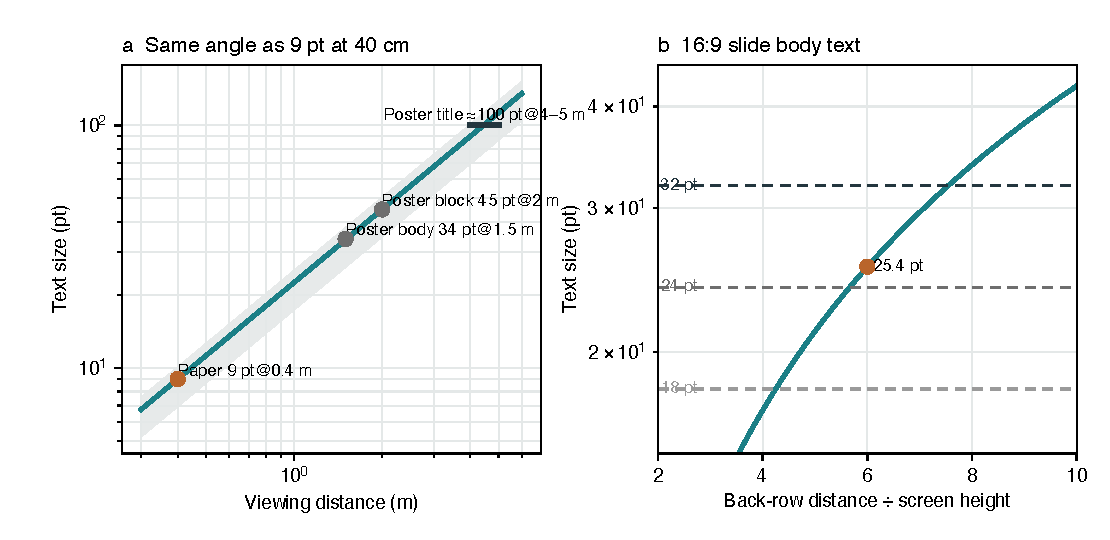
\includegraphics[width=\linewidth]{figures/ch12/ch12-02-visual-angle-text-size-en.pdf}
\caption{Text size from visual angle. Each curve gives the size that subtends the same angle as 9 pt text read at 40 cm. This is geometry, not a journal or conference rule; enlarge further for dim projection or less favourable viewing.}\label{fig:ch12-02}
\end{figure}

Let us walk through the four steps that produce the curves and benchmark markers in Figure~\ref{fig:ch12-02}.

\textbf{Step 1: Establish the desktop paper baseline.} When reading a printed journal issue or a tablet screen at a desk, a typical viewing distance is $d_0 = 40\ \text{cm} = 400\ \text{mm}$. A comfortable size for body text and clear figure annotations in print is $s_0 = 9\ \text{pt}$ (nominal body height $h_0 = 9 \times 0.3528 \approx 3.18\ \text{mm}$, with most journals setting $7\text{--}8\ \text{pt}$ as the lower floor for tick labels). Taking ``$9\ \text{pt}$ read at $40\ \text{cm}$'' as our reference benchmark gives a visual angle of:
\[
\theta_0 \approx \frac{3.18\ \text{mm}}{400\ \text{mm}} \approx 0.00794\ \text{rad} \approx 0.45^\circ
\]
If we translate the broader $7\text{--}10\ \text{pt}$ range common in published figures at $40\ \text{cm}$, the corresponding visual angle spans roughly $0.35^\circ\text{--}0.50^\circ$ (shown as the pale grey shaded band in Figure~\ref{fig:ch12-02}a). Note that ``$9\ \text{pt}$ at $40\ \text{cm}$'' is simply a convenient geometric reference chosen for mental arithmetic in this book, not a mandate from any publisher or standards body.

\textbf{Step 2: Scale poster text by physical viewing distance (Figure~\ref{fig:ch12-02}a).} Because an academic poster is laid out and printed at 1:1 physical dimensions (or at a known print scale factor), matching the visual angle of $9\ \text{pt}$ at $0.4\ \text{m}$ from a viewing distance $d$ (in meters) requires scaling the point size linearly with distance:
\[
s_{\text{poster}}(d) = 9 \times \frac{d}{0.4\ \text{m}}\ \text{pt} = 22.5\,d\ \text{pt}
\]
Substituting the three poster-hall viewing distances from Section 12.1 immediately yields target font sizes for the three information tiers:
\begin{itemize}
\item \textbf{Detail layer and close reading ($d = 1.0\text{--}1.5\ \text{m}$):} At $1.0\ \text{m}$, the equivalent size is $9 \times 1.0 / 0.4 = 22.5\ \text{pt}$; at $1.5\ \text{m}$---a natural distance when two or three colleagues stand side by side discussing a board---the equivalent size is $9 \times 1.5 / 0.4 = 33.75\ \text{pt} \approx 34\ \text{pt}$ (the lower grey dot in Figure~\ref{fig:ch12-02}a). Setting poster body bullets, axis titles, and tick labels between $28\ \text{pt}$ and $34\ \text{pt}$ ensures effortless reading at $1.5\ \text{m}$, while secondary methods notes and references meant for $0.5\text{--}1.0\ \text{m}$ inspection should never drop below $24\ \text{pt}$.
\item \textbf{Findings block headings ($d = 2.0\ \text{m}$):} So that a visitor standing two meters back or slightly down the aisle can grasp the takeaway sentence above each figure block at a glance, substituting $d = 2.0\ \text{m}$ gives $9 \times 2.0 / 0.4 = 45\ \text{pt}$ (the upper grey dot in Figure~\ref{fig:ch12-02}a).
\item \textbf{Top title banner ($d = 4.0\text{--}5.0\ \text{m}$):} To let passersby in the aisle read your research question from four to five meters away, substituting $d = 4.5\ \text{m}$ gives $9 \times 4.5 / 0.4 \approx 101\ \text{pt}$, spanning $90\text{--}113\ \text{pt}$ across the $4\text{--}5\ \text{m}$ interval (the dark horizontal bar near the top right of Figure~\ref{fig:ch12-02}a; notice how its text label \texttt{Poster title $\approx$100 pt@4--5 m} slightly crosses the right frame spine---a reminder to check label padding near plot borders).
\end{itemize}

\textbf{Step 3: Size slide text from the ratio of back-row distance to screen height (Figure~\ref{fig:ch12-02}b).} Projection slides differ from printed posters in one crucial respect: when you set type on a 16:9 slide in PowerPoint or Keynote, its physical height in the lecture hall depends entirely on the height $H$ of the venue's projection screen. Standard widescreen slide setups measure $13.333 \times 7.5\ \text{in}$ ($33.867 \times 19.05\ \text{cm}$), meaning the total vertical height of the slide canvas is fixed at $7.5 \times 72 = 540\ \text{pt}$. A font of nominal size $s_{\text{slide}}$ (in $\text{pt}$) therefore occupies a fraction $s_{\text{slide}} / 540$ of the screen height. If the physical screen height is $H$ and the back row sits at distance $D$, the visual angle subtended at the back row is:
\[
\theta \approx \frac{(s_{\text{slide}} / 540)\,H}{D} = \frac{s_{\text{slide}}}{540 \times (D/H)}
\]
Solving for $s_{\text{slide}}$ at our reference visual angle $\theta_0 \approx 0.45^\circ \approx 0.00785\ \text{rad}$ shows that the required slide font size depends only on the dimensionless ratio $D/H$ (back-row distance divided by screen height):
\[
s_{\text{slide}} \approx 0.00785 \times \left(\frac{D}{H}\right) \times 540\ \text{pt} \approx 4.24 \times \left(\frac{D}{H}\right)\ \text{pt}
\]
Two concrete examples show how this formula works in practice. First, consider a standard lecture hall with a screen height $H = 2.0\ \text{m}$ (width $\approx 3.56\ \text{m}$) and a back-row distance $D = 12\ \text{m}$, giving $D/H = 6$. On this screen, $24\ \text{pt}$ slide text occupies $24 / 540 = 1 / 22.5$ of the screen height ($\approx 8.9\ \text{cm}$ tall on the projection surface) and subtends $\approx 0.42^\circ$ at $12\ \text{m}$; matching $0.45^\circ$ exactly requires $25.4\ \text{pt}$ (the orange-brown dot in Figure~\ref{fig:ch12-02}b). This geometry explains a widely useful rule: \textbf{whenever the back row sits within roughly six screen heights of the display ($D/H \le 6$), $24\ \text{pt}$ is a safe floor for slide body text and axis titles, and tick labels should stay at or above $20\ \text{pt}$.}

Second, consider a long, low-ceilinged seminar room where the screen is only $H = 1.5\ \text{m}$ tall and the back table sits $D = 8\ \text{m}$ away ($D/H \approx 5.33$). If you drop figure labels to $18\ \text{pt}$ ($1/30$ of screen height), the visual angle at the back row shrinks to $(1.5 / 30) / 8 \approx 0.00625\ \text{rad} \approx 0.36^\circ$, right on the edge of the minimum legible floor in print. (As a practical graphic design note, inspect the left edge of Figure~\ref{fig:ch12-02}b: the reference labels \texttt{18 pt}, \texttt{24 pt}, and \texttt{32 pt} were placed flush against the left axis spine directly on top of the horizontal dashed lines; when labelling reference lines in your own charts, offset the text slightly above the dashed rule or into the right margin so the stroke never cuts through the numerals.)

\textbf{Step 4: Scale line weights and data markers in lockstep.} Visual angle governs curve strokes, axis spines, tick marks, and scatter symbols just as strictly as letterforms. On a printed journal page viewed at $40\ \text{cm}$, $0.5\text{--}0.8\ \text{pt}$ axis lines and $1.2\ \text{pt}$ data curves look crisp. Viewed from $1.5\ \text{m}$ on a poster, however, a $0.5\ \text{pt}$ hairline must be multiplied by $1.5 / 0.4 = 3.75$ to maintain the same apparent thickness. Data curves and axis spines on slides and posters should therefore be thickened to $2.0\text{--}3.5\ \text{pt}$. Whenever a room has a washed-out projector, strong ambient light, steep viewing angles from side aisles, or an international audience reading a second language, err on the side of larger type and heavier strokes than the bare geometric minimum.

\section{Turning a Paper Figure into a Slide Sequence}

With those geometric principles in hand, let us return to Zhou's perovskite solar cell study. We begin by inspecting the finalized manuscript version of Figure 2 from Chapter 9 (Figure~\ref{fig:ch12-03}) to see why a design that excels on a journal page breaks down when pasted onto a slide.

\begin{figure}[htbp]\centering
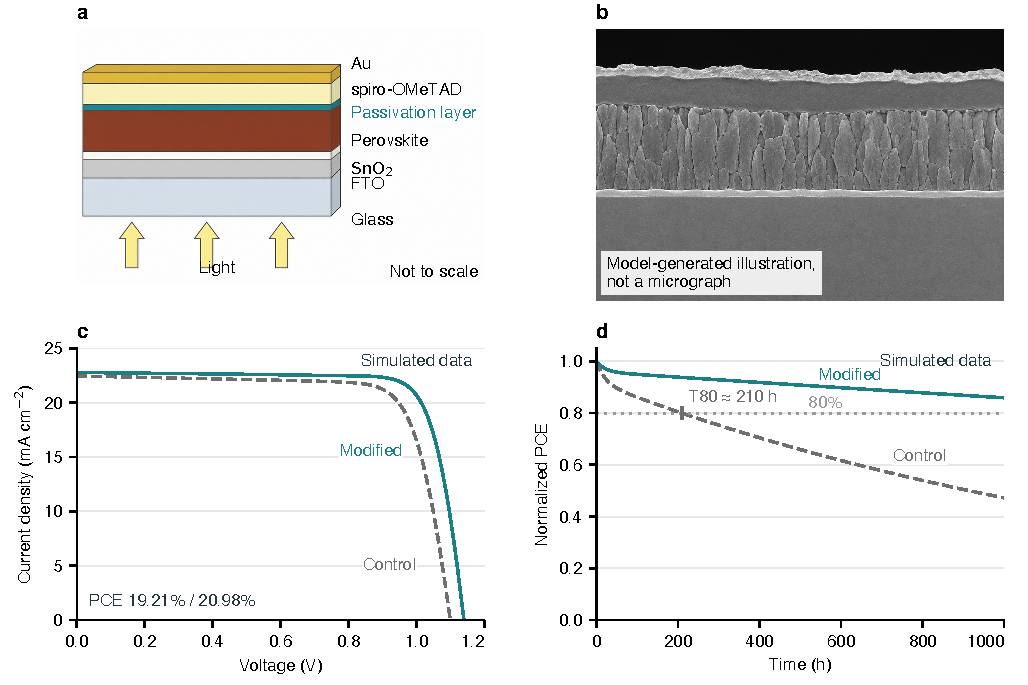
\includegraphics[width=\linewidth]{figures/ch12/ch12-03-paper-figure-2-en.pdf}
\caption{The paper version of Figure 2 (Chapter 9). Panels c and d show simulated data; panel b is a model-generated illustration, not a micrograph; panel a is not to scale.}\label{fig:ch12-03}
\end{figure}

In Figure~\ref{fig:ch12-03}, four panels fit cleanly inside a $174 \times 116\ \text{mm}$ double-column canvas: panel a diagrams the seven-layer stack ($\text{Glass}$, $\text{FTO}$, $\text{SnO}_2$, $\text{Perovskite}$, the teal $\text{Passivation layer}$, $\text{spiro-OMeTAD}$, and $\text{Au}$) with ``Not to scale'' at the bottom right; panel b shows a greyscale cross-sectional SEM-like texture with a light white box at the lower left explicitly stating ``Model-generated illustration, not a micrograph''; and panels c and d plot the simulated $J\text{--}V$ curves and $1000\ \text{h}$ normalized PCE stability traces using a grey dashed curve for the control device, a solid teal curve for the modified device, and ``Simulated data'' in the upper right corner. Yet when Zhou drops Figure~\ref{fig:ch12-03} wholesale onto a 16:9 slide and views it from the back row of the lecture hall, the audience sees Figure~\ref{fig:ch12-05}a.

\begin{figure}[htbp]\centering
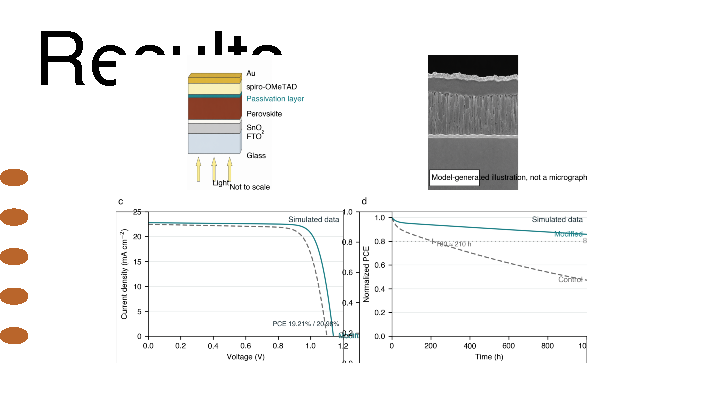
\includegraphics[width=119mm]{figures/ch12/ch12-05a-pasted-en.pdf}\\[1mm]
{\footnotesize (a) The paper figure pasted directly onto a slide: orange-brown markers (1)--(5) along the left margin flag the five defects analyzed in the text}\\[3mm]
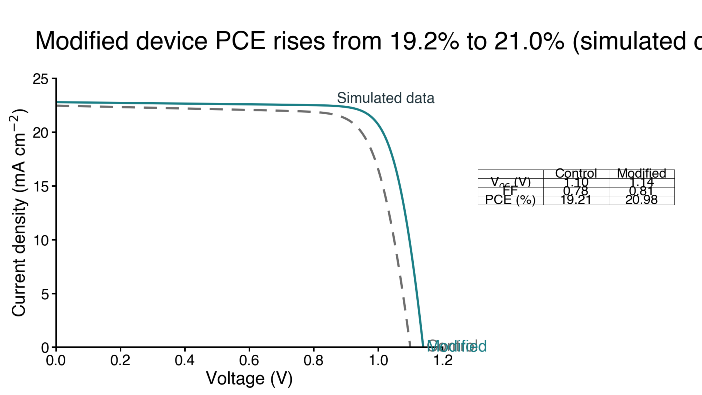
\includegraphics[width=119mm]{figures/ch12/ch12-05b-rebuilt-en.pdf}\\[1mm]
{\footnotesize (b) Slide 2b rebuilt for oral presentation: one question, an assertion headline, and large direct labels}
\caption{What the back row sees. Both slides are printed 119 mm wide; read at 40 cm, they subtend the same angle as a 3.6 m screen seen from 12 m. (a) The paper figure pasted in; (b) rebuilt for the talk. Simulated data.}\label{fig:ch12-05}\label{fig:ch12-05a}\label{fig:ch12-05b}
\end{figure}

The print width of Figure~\ref{fig:ch12-05} is calibrated to reproduce the exact visual angle of the back row: viewing a $3.56\ \text{m}$ wide 16:9 screen from $12\ \text{m}$ away subtends the exact same horizontal angle as viewing a $119\ \text{mm}$ wide image on this book page from $40\ \text{cm}$ ($3.56 / 12 \times 400\ \text{mm} \approx 119\ \text{mm}$). Held at normal reading distance, Figure~\ref{fig:ch12-05}a and Figure~\ref{fig:ch12-05}b show what a listener in row twelve actually experiences. Following the five orange-brown numbered circles (1)--(5) down the left margin of Figure~\ref{fig:ch12-05}a (notice that even the white numerals inside those margin circles are oversized and clipped by the circle borders), we can diagnose five concrete failures of the pasted-figure slide:
\begin{enumerate}
\item \textbf{Illegible tick labels and axis titles (marker 1):} Scaling a $174\ \text{mm}$ figure set in $8\ \text{pt}$ type (or a $180\ \text{mm}$ figure set in $7\ \text{pt}$ type) to $90\%$ of a 16:9 slide width ($\approx 305\ \text{mm}$) yields an effective slide font size of only $12\text{--}14\ \text{pt}$. At $12\ \text{m}$, those characters subtend just $0.21^\circ\text{--}0.25^\circ$---less than half the visual angle of normal paper reading---leaving the voltage and current-density scales unreadable from the back half of the room.
\item \textbf{Cramped annotations, colliding axes, and hard-to-trace curves (marker 2):} When a paper plot uses a corner legend box, listeners have to dart back and forth between legend keys and curves. Even when the paper plot uses direct labels, squeezing all four panels into a tight slide viewport causes severe collisions in Figure~\ref{fig:ch12-05}a: the right frame spine of panel c cuts straight through the vertical axis tick labels (\texttt{1.0}, \texttt{0.8}, \texttt{0.6}, \texttt{0.4}, \texttt{0.2}, \texttt{0.0}) of panel d; in the bottom-right corner of panel c, \texttt{Control} and \texttt{Modified} pile directly on top of each other and crash into the \texttt{1.2} tick mark; in panel d, \texttt{T80 $\approx$ 210 h} sits right across the grey dashed trace; and in panel a, \texttt{Light} collides with \texttt{Not to scale}.
\item \textbf{Four panels competing for attention at once (marker 3):} Projecting all four panels simultaneously splits the room's focus---while the speaker explains the $J\text{--}V$ sweep in panel c, half the audience is still deciphering the layer stack in panel a or squinting at panel b. Careless subplot placement also clips the outer edges: the top panel letters \texttt{a} and \texttt{b} are sliced off, and the rightmost horizontal tick \texttt{1000} in panel d is truncated to \texttt{10}.
\item \textbf{A topic label instead of a finding in the title bar (marker 4):} The heading \texttt{Results} in the upper left tells the audience nothing about what the study found (and in Figure~\ref{fig:ch12-05}a, the top of panel a's bounding box slices off the lower half of the word \texttt{Results}).
\item \textbf{Compromised or missing provenance disclosures (marker 5, highest integrity risk):} Because the manuscript figure legend is absent from the slide, the simulation conditions disappear. Worse, in panel b's lower-left disclaimer \texttt{Model-generated illustration, not a micrograph}, the white backing rectangle is too narrow, so \texttt{ed illustration, not a micrograph} spills out in black text across the dark grey cross-section and right margin, making it nearly invisible from the back row and inviting listeners to mistake a generative texture for an actual electron micrograph.
\end{enumerate}

Transforming Figure~\ref{fig:ch12-03} into a sequence of slides that read clearly from the back row (as in Figure~\ref{fig:ch12-05}b) follows a six-step workflow that converts spatial panels into a temporal narrative (Figure~\ref{fig:ch12-04}).

\begin{figure}[htbp]\centering
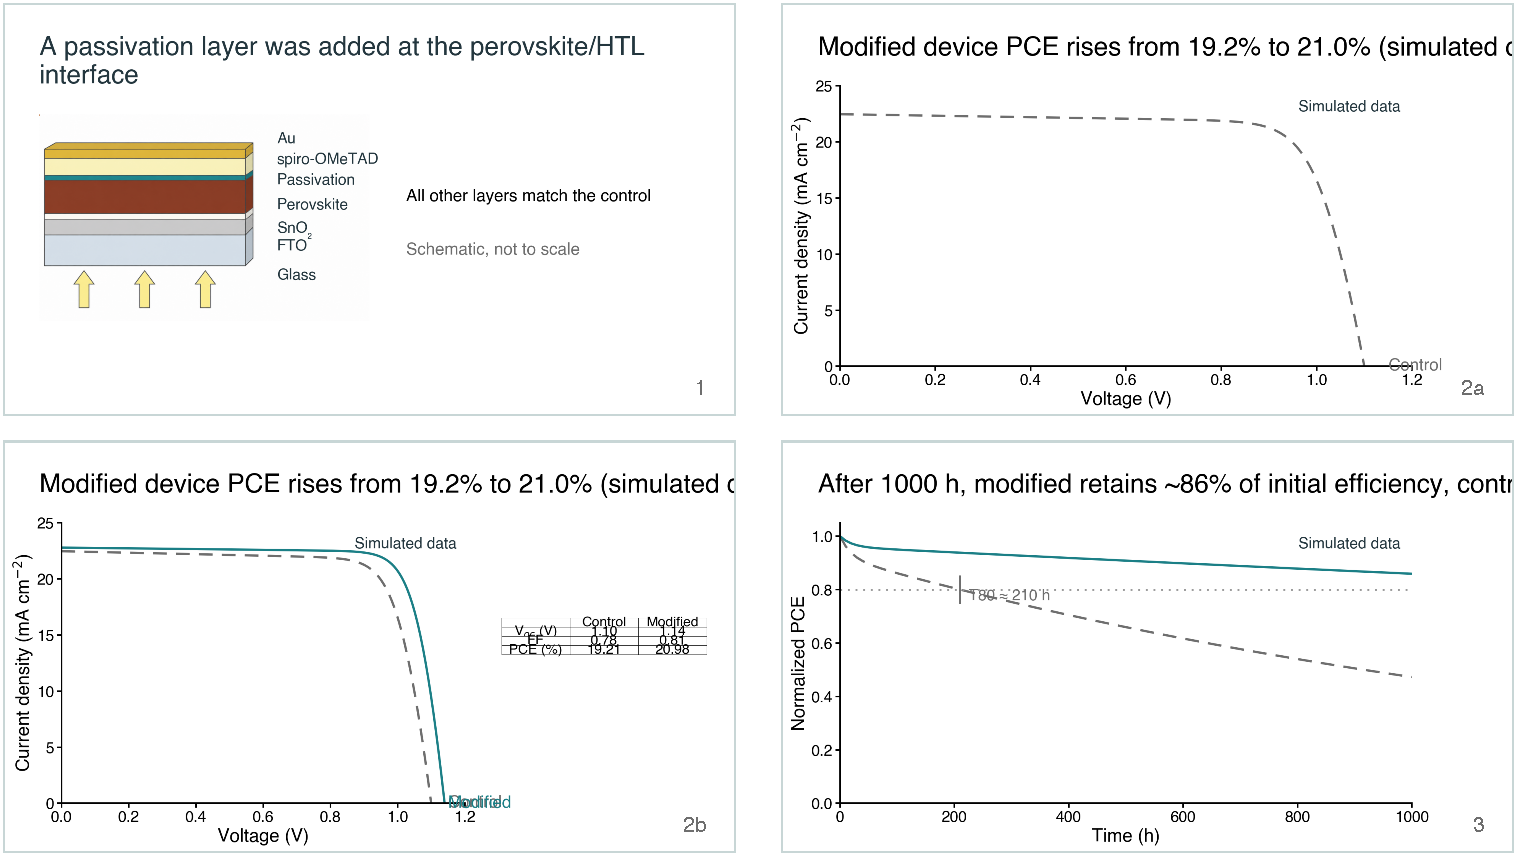
\includegraphics[width=\linewidth]{figures/ch12/ch12-04-slide-sequence-en.pdf}
\caption{Three talk slides built from the same data (slide 2 revealed in two steps). Each title states the finding, curves are labelled directly, and values, axis ranges and colour meanings match the paper figure. Simulated data.}\label{fig:ch12-04}
\end{figure}

\textbf{Step 1: List the sub-questions answered by the composite figure and move secondary panels to backup slides.} Figure 2 of the manuscript answers three sequential questions: (1) What physical change did we make to the device stack? (2) How much did that change raise initial photovoltaic efficiency? (3) How well did the modified device retain its efficiency over $1000\ \text{h}$ of operation? Because the cross-sectional illustration in panel b is a conceptual visual placeholder rather than primary quantitative evidence, it does not belong in the three-minute core talk flow; move it---together with its prominent ``Model-generated illustration, not a micrograph'' label---to a backup slide at the end of the deck for Q\&A.

\textbf{Step 2: Dedicate one slide to each sub-question and write an assertion headline.} Following the assertion--evidence structure widely used in scientific speaking (Naegle, 2021), replace generic headers like ``Results'' with a full $32\text{--}36\ \text{pt}$ sentence stating the takeaway and data status: Slide 1 reads ``A passivation layer was added at the perovskite/HTL interface''; Slide 2 reads ``Modified device PCE rises from $19.2\%$ to $21.0\%$ (simulated data)''; and Slide 3 reads ``After $1000\ \text{h}$, modified retains $\sim 86\%$ of initial efficiency, control $\sim 47\%$ (simulated data)''.

\textbf{Step 3: Use progressive reveal to pace complex comparisons.} Split Slide 2 into two identically registered frames (Slide 2a and Slide 2b in Figure~\ref{fig:ch12-04}). When Slide 2a first appears, only the axes and the grey dashed \texttt{Control} curve are visible, giving the speaker ten seconds to orient the room to the voltage and current-density scales. Advancing to Slide 2b (reproduced at back-row scale in Figure~\ref{fig:ch12-05}b) overlays the solid teal \texttt{Modified} curve on the exact same axis limits and reveals a compact summary table ($V_{\text{oc}}$, $\text{FF}$, and $\text{PCE}$) on the right. Because the axis bounding box never shifts between 2a and 2b, the eye immediately registers the outward expansion of the $J\text{--}V$ knee.

\textbf{Step 4: Strip away panel letters and detached legends in favor of direct callouts.} Delete the manuscript panel letters \texttt{a}--\texttt{d} and separate legend boxes. Label each curve directly by name, highlight the ultrathin passivation layer on Slide 1 with a bold orange-brown outline, and place just two short explanatory lines on the right of Slide 1 (``All other layers match the control'' and ``Schematic, not to scale'').

\textbf{Step 5: Redraw natively at 16:9 dimensions and audit the full-size export for text collisions.} Render every slide natively on a $13.333 \times 7.5\ \text{in}$ widescreen canvas (title $34\ \text{pt}$, axis titles $24\ \text{pt}$, tick labels $20\ \text{pt}$, annotations $22\ \text{pt}$, curve strokes $3\ \text{pt}$) rather than stretching a square or 4:3 plot. Crucially, always inspect the exported slides at full screen before walking into the seminar room. Examining the actual rendered frames in Figure~\ref{fig:ch12-04} and Figure~\ref{fig:ch12-05}b reveals four typographic flaws that an author must fix in presentation software or in the plotting script: (1) while Slide 1 wrapped its two-line title cleanly, the single-line $34\ \text{pt}$ titles on Slides 2a, 2b, and 3 are too long for the canvas width and get clipped at the right border (\texttt{... (simulated d} and \texttt{... contr})---insert a manual line break or reduce the title to $30\text{--}32\ \text{pt}$; (2) on Slides 2a and 2b (and Figure~\ref{fig:ch12-05}b), anchoring the direct labels \texttt{Control} and \texttt{Modified} to the final data point ($J = 0$) drops both words right onto the horizontal axis spine between $1.1\ \text{V}$ and $1.2\ \text{V}$ where they overwrite each other---move both labels upward into the open whitespace beside the steep descending knee of each curve; (3) on Slide 2b, the small summary table drawn by the plotting library has cramped vertical row height so \texttt{V\textsubscript{oc} (V)} and \texttt{FF} crowd the horizontal cell rules---building that three-row table natively in PowerPoint or Keynote gives much cleaner padding; and (4) on Slide 3, the \texttt{T80 $\approx$ 210 h} label sits directly across the grey dashed trace and the $0.8$ dotted reference line, and direct \texttt{Control}/\texttt{Modified} curve labels still need to be added above and below the traces.

\textbf{Step 6: Lock data values, axis ranges, colour semantics, and provenance notes across versions.} Keep every metric, axis range ($0\text{--}1.2\ \text{V}$, $0\text{--}25\ \text{mA cm}^{-2}$, $0\text{--}1000\ \text{h}$; if you ever zoom in on a sub-range, state that crop explicitly on the slide and in your spoken remarks), grey-dashed versus solid-teal encoding, and in-plot \texttt{Simulated data} tag identical to the manuscript figure.

\section{An A0 Portrait Poster: Grid, Hierarchy, and Density}

Under the ISO 216 international paper standard, an \textbf{A0 portrait poster} measures $841 \times 1189\ \text{mm}$---an area of exactly $1\ \text{m}^2$. Before dividing up that square meter of paper, consider how colleagues actually move through a conference poster hall (Figure~\ref{fig:ch12-07}).

\begin{figure}[htbp]\centering
\begin{tikzpicture}
\node[anchor=south west,inner sep=0] (img) at (0,0) {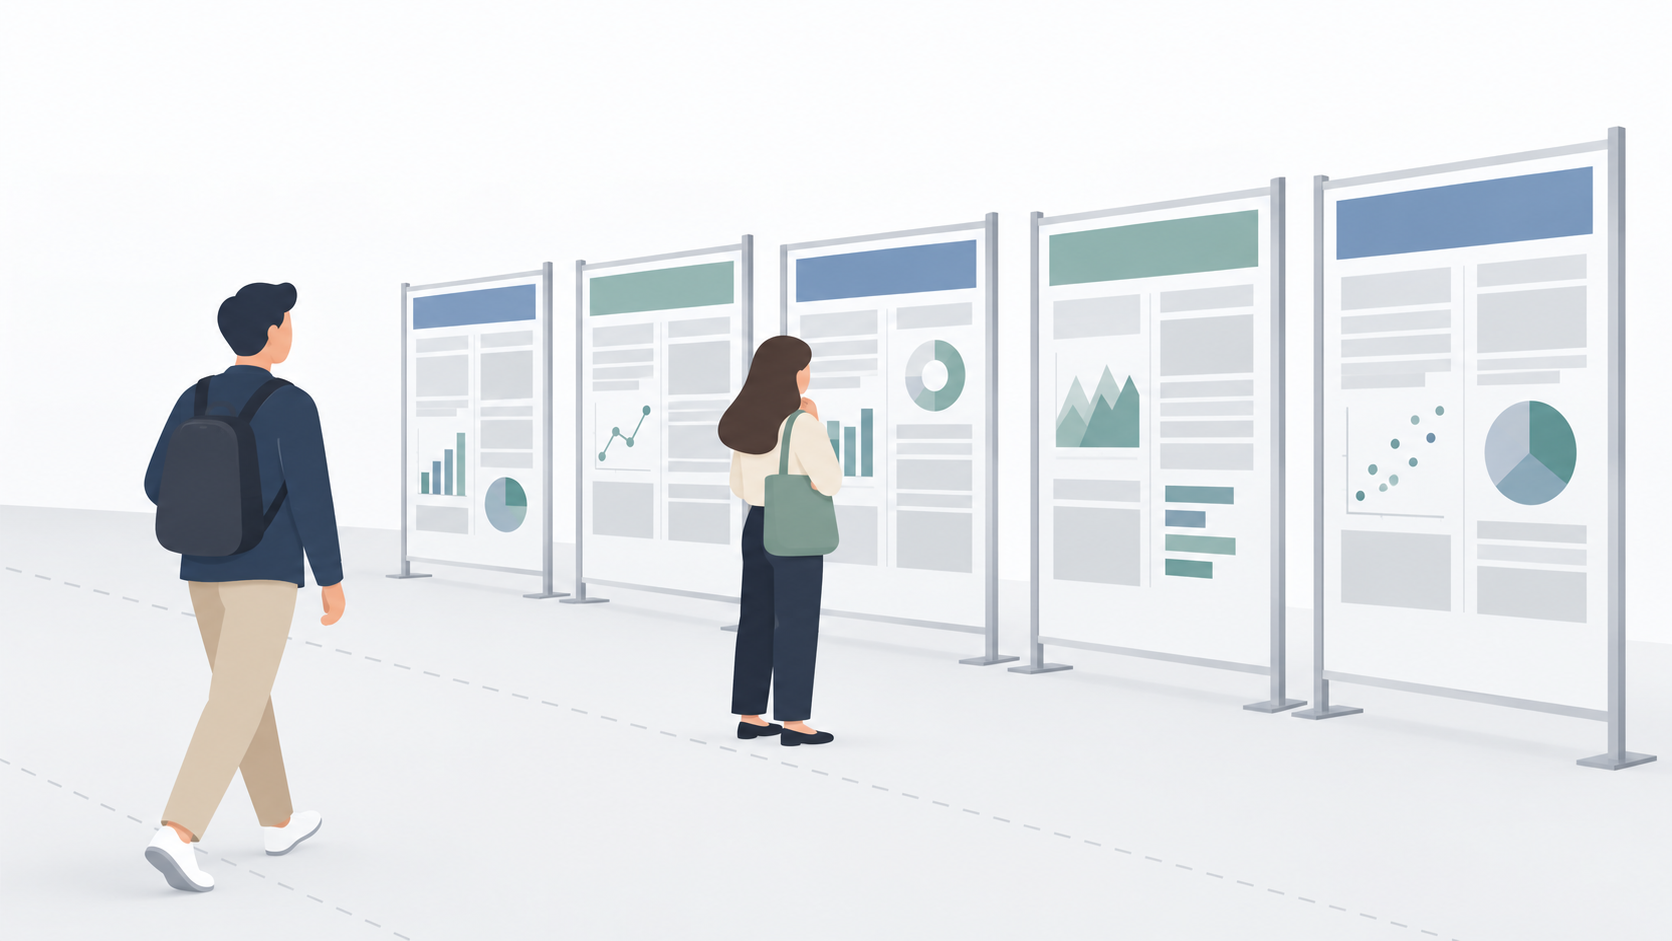
\includegraphics[width=\linewidth]{figures/ch12/ch12-07-poster-hall-distances.png}};
\begin{scope}[x={(img.south east)},y={(img.north west)}]
  \node[font=\footnotesize,fill=white,fill opacity=0.88,text opacity=1,inner sep=2pt] at (0.18,0.12) {About 3--5 m: title and main finding};
  \node[font=\footnotesize,fill=white,fill opacity=0.88,text opacity=1,inner sep=2pt] at (0.58,0.12) {About 1 m: evidence and detail};
\end{scope}
\end{tikzpicture}
\caption{A poster is seen from afar before it is read up close. Illustration; figures and distances are not to scale (base illustration generated by an image model with distance labels overlaid by the author; prompts and generation records are available in the book repository).}\label{fig:ch12-07}
\end{figure}

When we generated the text-free base illustration for Figure~\ref{fig:ch12-07} from an English prompt, we ran the same prompt three times to get the spatial cues right: the first run drew the two faint dashed floor lines at sharply diverging angles, and the second run routed the outer dashed line behind the walking attendee's heels rather than beside their feet. The third run (Figure~\ref{fig:ch12-07}) aligned the two dashed floor lines with the two viewing positions---one passing the attendee walking down the aisle in the left foreground, the other passing just in front of the colleague standing close to the middle board---while keeping all five poster boards strictly abstract with teal/slate header bands, two-column grey rectangles, and unlabelled chart shapes (the row of boards spans roughly the right three-quarters of the frame with subtle soft shading, and the English distance callouts are overlaid in TikZ). That two-stage encounter---scanning from $3\text{--}5\ \text{m}$ in the aisle before stepping in to $1\ \text{m}$---governs every layout decision on an A0 poster (Figure~\ref{fig:ch12-06}).

\begin{figure}[htbp]\centering
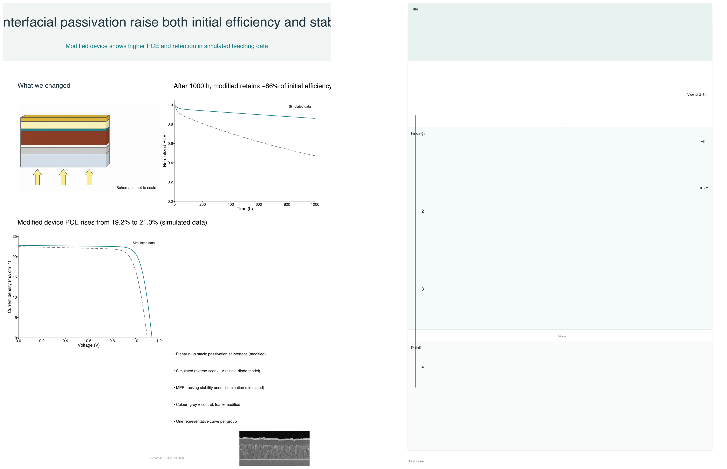
\includegraphics[width=\linewidth]{figures/ch12/ch12-06-a0-poster-layout-en.pdf}
\caption{An A0 portrait poster (841 $\times$ 1189 mm), final layout and wireframe. The three layers are written for reading at 3--5 m, 1--2 m and 0.5 m; plots were redrawn for viewing at 1.5 m. Simulated data; the cross-section is a model-generated illustration.}\label{fig:ch12-06}
\end{figure}

Comparing the rendered layout on the left of Figure~\ref{fig:ch12-06} with its structural wireframe on the right highlights three core design rules:
\begin{enumerate}
\item \textbf{A two-column grid with top-to-bottom column-wise reading order:} Leave a $30\ \text{mm}$ outer margin around all four edges (always $\ge 25\ \text{mm}$ so nothing is lost to printer bleed or poster-board clips), place a full-width $150\ \text{mm}$ title banner across the top, and divide the main body into two equal columns separated by a $20\ \text{mm}$ gutter (typically $15\text{--}20\ \text{mm}$), giving each column a net width of $380.5\ \text{mm}$. Organize the reading sequence vertically down the left column first (block 1 to block 2) and then down the right column (block 3 to block 4, following the vertical arrow on the wireframe), so a visitor standing in front of the board never has to zig-zag back and forth across nearly a meter of width after every panel (Erren and Bourne, 2007).
\item \textbf{Three distance tiers and a deliberate reassignment of the four manuscript panels:}
  \begin{itemize}
  \item \textbf{Title band (for $3\text{--}5\ \text{m}$ viewing):} Set inside a pale teal-grey banner at the top, the primary line asks the study question in $96\ \text{pt}$ type, while the second line states the main takeaway in $44\ \text{pt}$ teal type: ``Modified device shows higher PCE and retention in simulated teaching data''.
  \item \textbf{Findings layer (for $1\text{--}2\ \text{m}$ viewing):} Three large blocks occupy the upper and middle zones: top-left ``What we changed'' (device stack schematic M1 with a $28\ \text{pt}$ ``Schematic, not to scale'' note), bottom-left efficiency ($J\text{--}V$), and top-right operational stability. Each data block opens with a $48\ \text{pt}$ assertion heading above a plot redrawn specifically for $1.5\ \text{m}$ viewing (axis titles $32\ \text{pt}$, tick labels $28\ \text{pt}$, curve strokes $3.5\ \text{pt}$, and in-plot ``Simulated data'' note at $24\ \text{pt}$).
  \item \textbf{Detail layer (for $0.5\ \text{m}$ viewing):} The bottom-right zone groups five concise $28\ \text{pt}$ methodological bullets (planar n-i-p stack, single-diode reverse-scan model, MPP tracking condition, grey/teal colour key, and single representative curve notice) alongside a demoted thumbnail of panel b's cross-sectional illustration M2 carrying its $24\ \text{pt}$ provenance disclaimer.
  \end{itemize}
  Just as with the slides, inspecting the full-size A0 proof in Figure~\ref{fig:ch12-06} (left) at $100\%$ scale catches four layout items that must be cleaned up before sending the PDF to the print shop: (1) the centered $96\ \text{pt}$ question in the top banner (``Can interfacial passivation raise both initial efficiency and stability?'') exceeds the $841\ \text{mm}$ page width on a single line and gets clipped at both left and right margins (\texttt{nterfacial passivation raise both initial efficiency and stab})---wrap it onto two lines of $84\text{--}90\ \text{pt}$; (2) the $48\ \text{pt}$ assertion heading above the top-right stability block overflows the right margin (\texttt{... initial efficiency}) and needs a line break before ``control $\sim 47\%$''; (3) the device stack M1 and the two data plots need their $36\ \text{pt}$ layer names and direct \texttt{Control}/\texttt{Modified} curve labels added in the open canvas space; and (4) at the bottom edge of the M2 cross-section thumbnail in the lower-right corner, the dark text \texttt{Model-generated illustration, not a micrograph} sits directly over the dark grey substrate where it is clipped and hard to read---place it inside a light semi-transparent backing box just above the bottom edge.
\item \textbf{Density self-checks and the squint test:} Instead of aiming for an arbitrary word count, apply a five-minute reading test: can a colleague standing at $1.5\ \text{m}$ read every word on the poster in under five minutes while leaving generous open background around each plot? Then run the \textbf{squint test} (or thumbnail-and-blur test): shrink the poster to $12\ \text{cm}$ high and apply a Gaussian blur ($\sigma \approx 1.5\ \text{mm}$ at thumbnail scale) to simulate what the eye perceives from down the aisle (Figure~\ref{fig:ch12-08}).
\end{enumerate}

\begin{figure}[htbp]\centering
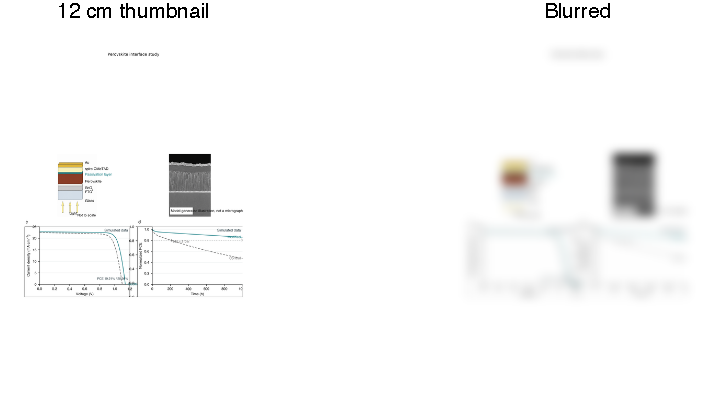
\includegraphics[width=\linewidth]{figures/ch12/ch12-08a-dense-squint-en.pdf}\\[1mm]
{\footnotesize (a) Crowded draft C0: three columns of manuscript prose above an enlarged copy of the four-panel paper figure}\\[3mm]
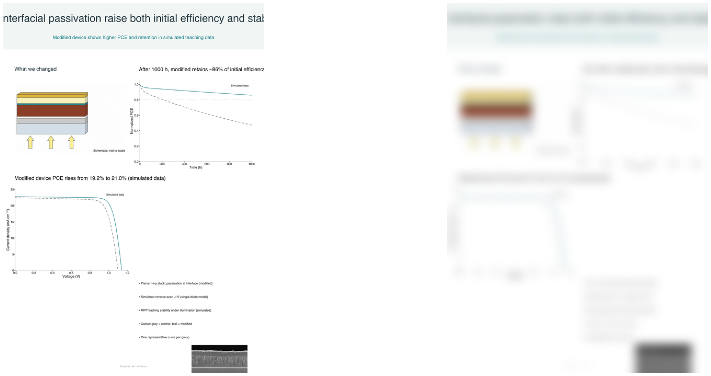
\includegraphics[width=\linewidth]{figures/ch12/ch12-08b-focused-squint-en.pdf}\\[1mm]
{\footnotesize (b) Layered final layout: top title banner, three findings blocks, and lower-right detail zone}
\caption{The squint test. Left: a 12 cm thumbnail; right: the same, blurred. (a) The crowded draft turns into an even grey; (b) the final layout keeps its title band and three blocks.}\label{fig:ch12-08}\label{fig:ch12-08a}\label{fig:ch12-08b}
\end{figure}

Compare Figure~\ref{fig:ch12-08}a and Figure~\ref{fig:ch12-08}b. In the crowded draft C0 (Figure~\ref{fig:ch12-08}a), the top of the board has only a small $36\ \text{pt}$ heading (\texttt{Perovskite interface study}) with no colored banner or main finding; the upper half is filled with five sections of $20\ \text{pt}$ manuscript prose across three columns (roughly 140 words in this sample mockup, which already fade to near-invisibility at $12\ \text{cm}$ thumbnail height); and the middle of the board simply enlarges the $174\ \text{mm}$ manuscript Figure 2 by roughly $4\times$ across the page (turning $0.6\ \text{pt}$ lines into $\sim 2.4\ \text{pt}$, which is passable, but scaling $8\ \text{pt}$ labels to $\sim 32\ \text{pt}$ with panels c and d still colliding, erasing any visual hierarchy between section headings and tick labels). Once blurred, C0 collapses into a featureless pale field above four indistinct smudges. In the layered final layout (Figure~\ref{fig:ch12-08}b), even after Gaussian blurring (and even with the un-wrapped top title line), the top banner, the three findings blocks with their bold assertion bars, and the bottom-right detail zone remain unmistakable.

\section{Completing All Three Versions in SciDraw AI}

When producing the manuscript figure, the slide sequence, and the conference poster in \scidraw{}, route each task to the workspace designed for it and keep a clear boundary between what the platform automates and what you must finish and verify in local software:
\begin{itemize}
\item \textbf{Redrawing data plots at new aspect ratios and font sizes (Scientific Visualization \sdtool{sci-vis}):} Rather than starting from scratch or re-uploading your CSV files, open the history session from your Chapter 9 manuscript plot, select the verified final version, and submit a targeted revision instruction to generate a 16:9 slide version, a control-only build frame for progressive reveal, and a thick-stroked poster panel. The workspace supports multi-turn conversational editing, branching from historical versions, restoring the previous or original state, and exporting in multiple formats. Afterward, verify that every numerical value, axis limit, and colour mapping remained intact, and check the actual rendered point size after placing the graphic onto your PowerPoint slide or A0 poster canvas (Chapter 13 examines how to verify whether an exported file contains true editable vector paths).
\item \textbf{Slide decks and poster layout frameworks (Presentation Templates \path{/scientific-presentation-templates} and Poster Templates):} The presentation template library provides downloadable 16:9 PPTX frameworks tailored for thesis defenses, conference talks, literature seminars, group meetings, and proposal defenses. The poster template library offers three layout families---Classic, Focus, and Four-Column---across standard academic dimensions including A0 portrait, A0 landscape, A1, $36 \times 48\ \text{in}$, $90 \times 120\ \text{cm}$, and 16:9 digital e-posters (note that $72\ \text{in}$ wide posters are built at $50\%$ physical dimensions to stay within presentation software page-size limits and are printed at $200\%$ scale, as noted inside the template file). Keep the boundary clear: \textbf{downloading a PPTX template does not automatically populate your content}. \scidraw{} does not offer a one-click tool that converts a manuscript into a multi-slide editable presentation or a print-ready editable poster; you assemble your redrawn plots and assertion headlines inside PowerPoint or Keynote.
\item \textbf{Exploring overall poster visual directions (Scientific Poster Maker \path{/scientific-poster-maker}):} This generator produces a single bitmap concept image of a poster from a text prompt, and can also draft a visual prompt by reading an uploaded manuscript PDF (currently parsing only the first five pages, abstract, and opening text rather than comprehending the full paper). Use it strictly as a rough mood board to compare column proportions or accent palettes before you start laying out your template. \textbf{Never send a generated poster bitmap to the printer as your final poster}, and never keep any text or synthetic ``charts'' rendered inside that bitmap; always build the real poster in an editable template or deterministic script using verified figures and text.
\item \textbf{Unpacking composite panels and checking target print width (Multi-Panel Figure Maker \sdtool{multi-panel-figure-maker} and Figure Checker \sdtool{figure-checker}):} When you export a composite figure as PPTX from \sdtool{multi-panel-figure-maker}, each panel bitmap and its panel letter (\texttt{a}, \texttt{b}, \dots) are stored as separate slide objects, making it easy to lift out the device schematic in panel a or delete the panel letters. However, the curves, axes, and labels inside each panel bitmap are not individually editable vector objects, so data panels still need to be redrawn at slide or poster font sizes in \sdtool{sci-vis} or your plotting script. Once assembled, run \sdtool{figure-checker} at your target physical width to audit effective resolution (ppi), greyscale contrast, and colour-vision deficiency risks---remembering that visual-angle legibility, reading order, and scientific accuracy remain the author's responsibility. Because tools do not automatically pipe files across workspaces, pass assets between stages by downloading clearly named files and importing them into the next step.
\end{itemize}

\section{Worked Case: One Study, Three Versions}

We now bring together the complete closed-loop record for our perovskite solar cell interfacial-passivation case: raw materials and simulation parameters, the three drawing briefs, copy-ready revision prompts, spoken narration and poster captions, and the cross-version consistency audit.

\textbf{1. Study setup and simulated data parameters.} This teaching case compares a planar n-i-p perovskite solar cell (control) against an otherwise identical stack incorporating an ultrathin interfacial passivation layer between the perovskite absorber and the hole transport layer (modified). No real experimental device measurements are reported; all numerical curves are generated deterministically from a standard single-diode equation and a two-term exponential decay model. Illuminated through the glass substrate, the stack sequence from bottom to top is: $\text{Glass}$ / $\text{FTO}$ / $\text{SnO}_2$ ($\sim 30\ \text{nm}$) / perovskite absorber ($\sim 500\ \text{nm}$) / interfacial passivation layer (modified group only, ultrathin) / $\text{spiro-OMeTAD}$ ($\sim 200\ \text{nm}$) / $\text{Au}$ back contact ($\sim 80\ \text{nm}$), without specifying a particular chemical formula for the perovskite composition or passivating molecule.

Across the four source materials, M1 is the layer-stack schematic (not to scale); M2 is a model-generated cross-sectional SEM-like texture (in an actual research paper, cross-sectional morphology must come from real electron microscopy of the same device batch with calibrated scale bars and unaltered raw backups as covered in Chapter 8; we use a generative texture here solely as a layout placeholder because no real micrograph exists for a simulated device, and every derived version must carry the explicit notice ``Model-generated illustration, not a micrograph''); M3 is the simulated reverse-scan $J\text{--}V$ dataset under AM1.5G illumination ($100\ \text{mW cm}^{-2}$) at $25\ ^\circ\text{C}$ solved from $J = J_L - J_0[\exp((V + J R_s)/(n V_T)) - 1] - (V + J R_s)/R_{\text{sh}}$ with $V_T = 0.025693\ \text{V}$ (a single scan direction is simulated without hysteresis; on $J\text{--}V$ hysteresis see Snaith et al., 2014, and on detailed-balance efficiency limits see Shockley and Queisser, 1961), where the control group ($J_L = 22.5\ \text{mA cm}^{-2}$, target $V_{\text{oc}} = 1.10\ \text{V}$, $n = 1.6$, $R_s = 2.5\ \Omega\cdot\text{cm}^2$, $R_{\text{sh}} = 1500\ \Omega\cdot\text{cm}^2$) yields $J_{\text{sc}} = 22.46\ \text{mA cm}^{-2}$, $V_{\text{oc}} = 1.100\ \text{V}$, $\text{FF} = 0.777$, and $\text{PCE} = 19.21\%$, and the modified group ($J_L = 22.8\ \text{mA cm}^{-2}$, target $V_{\text{oc}} = 1.14\ \text{V}$, $n = 1.5$, $R_s = 2.0\ \Omega\cdot\text{cm}^2$, $R_{\text{sh}} = 3000\ \Omega\cdot\text{cm}^2$) yields $J_{\text{sc}} = 22.78\ \text{mA cm}^{-2}$, $V_{\text{oc}} = 1.140\ \text{V}$, $\text{FF} = 0.808$, and $\text{PCE} = 20.98\%$; and M4 is the $0\text{--}1000\ \text{h}$ normalized PCE stability trace simulated for continuous 1-sun illumination with maximum-power-point (MPP) tracking in $\text{N}_2$ at $\sim 25\ ^\circ\text{C}$ (for consensus stability reporting protocols see Khenkin et al., 2020), where the control trace $y(t) = [1 - 0.08(1 - e^{-t/20})]e^{-t/1500}$ reaches $T_{80} = 210\ \text{h}$ and retains $0.47$ of its initial efficiency at $1000\ \text{h}$, while the modified trace $y(t) = [1 - 0.04(1 - e^{-t/20})]e^{-t/9000}$ stays above $0.80$ throughout the $1000\ \text{h}$ window ($T_{80} > 1000\ \text{h}$) and retains $0.86$ at $1000\ \text{h}$.

\textbf{2. The three drawing briefs.} Each version is governed by its own explicit brief before any redrawing begins.

Brief A (Manuscript Figure 2):
\begin{Prompt}
[Purpose & Audience] Manuscript Figure 2 for photovoltaic and materials peers;
read independently at ~40 cm; pace controlled by the reader.
[One-Sentence Goal] Readers can see that interfacial passivation improves both
initial efficiency and 1000 h stability over the control, and can locate Jsc,
Voc, FF, PCE, and T80.
[Panels] a device stack schematic; b cross-section texture (model-generated);
c simulated J-V curves; d simulated normalized PCE vs. time.
[Dimensions] Double-column 174 mm width, 8 pt in-panel labels, 10 pt bold
lowercase panel letters.
[Fixed Constraints] All values from the master metrics table; control = grey
#6E6E6E dashed, modified = teal #1B7F86 solid.
[Disclosures] Panels c, d labeled "Simulated data"; panel b labeled
"Model-generated illustration, not a micrograph"; panel a "Not to scale".
\end{Prompt}

Brief B (Group-meeting / conference talk sequence, 3 slides at 16:9):
\begin{Prompt}
[Purpose & Audience] 3-minute results segment in a 10-minute talk for group
members and materials peers; screen height ~2 m, back row 10-12 m; pace
controlled by the speaker.
[One-Sentence Goal] Listeners grasp in three sequential steps: what layer was
added -> how much initial efficiency rose -> how much 1000 h stability improved.
[Slide Plan]
  Slide 1 Title: "A passivation layer was added at the perovskite/HTL interface".
          Enlarged device schematic (M1) with passivation layer highlighted;
          cross-section texture M2 moved to backup slide with full disclaimer.
  Slide 2 Title: "Modified device PCE rises from 19.2% to 21.0% (simulated data)".
          Two-step reveal: (2a) axes + control curve; (2b) add modified curve +
          compact Voc/FF/PCE table; direct curve labels, no detached legend box.
  Slide 3 Title: "After 1000 h, modified retains ~86% of initial efficiency,
          control ~47% (simulated data)". Stability curves with 0.8 line & T80.
[Specs & Check] 16:9 (33.867 x 19.05 cm); ticks >= 20 pt, axis titles >= 24 pt,
slide titles 32-36 pt, lines >= 2.5 pt, no panel letters. Readable at 1/4 scale.
\end{Prompt}

Brief C (A0 portrait conference poster):
\begin{Prompt}
[Purpose & Audience] Conference poster hall, A0 portrait (841 x 1189 mm);
passersby scan from 2-5 m, visitors read at 0.5-1.5 m for 3-5 min; presenter
may not be present.
[One-Sentence Goal] Passersby read the question and main finding from 3 m;
closer visitors read "what changed -> efficiency -> stability" and key methods.
[Hierarchy] Title band: question + main finding (title >= 90 pt); Findings
layer: 3 blocks, each with an assertion heading (>= 44 pt) + redrawn figure;
Detail layer: 5 method bullets, M2 thumbnail + disclaimer (body >= 28 pt, min 24 pt).
[Grid & Order] 2 columns, 30 mm outer margin, 20 mm column gap; top-to-bottom
column-wise order: Banner -> Left-top (stack) -> Left-bottom (J-V) ->
Right-top (stability) -> Right-bottom (methods & M2 detail).
[Plots & Check] Redraw plots for 1.5 m viewing (ticks >= 28 pt, lines >= 3 pt).
Passes 12 cm blurred squint test and 1:1 A4 patch test at 1.5 m.
\end{Prompt}

\textbf{3. Copy-ready revision prompts and poster layout prompt.} Opening the Chapter 9 $J\text{--}V$ history session in \sdtool{sci-vis} and selecting the verified manuscript plot, submit the following revision instruction:
\begin{Prompt}
Keep all data points, both group colours (control #6E6E6E dashed, modified
#1B7F86 solid), the horizontal axis 0-1.2 V, and the vertical axis 0-25 mA/cm2
unchanged, and generate a version for a 16:9 presentation slide:
1. 16:9 canvas with the plot occupying roughly the left 60% of the frame;
2. Tick labels equivalent to 20 pt and axis titles 24 pt on a 33.867 cm wide
   slide; curve stroke width 3 pt;
3. Remove the legend box and label "Control" and "Modified" directly in the
   open space beside the descending knee of each curve (do not overlap y = 0);
4. Place "Simulated data" inside the upper right corner of the plot area;
5. Do not add any new numbers, error bars, or significance markers.
Also export a control-only frame with identical axis bounds for step-by-step reveal.
\end{Prompt}

After export, verify that the two reveal frames share identical pixel coordinates for the axis box so nothing jumps on click, confirm that every number matches the master metrics file, and check that the tool did not smooth the curves or alter the hex colours. To generate the poster $J\text{--}V$ plot, run the same prompt with item 2 adjusted to: ``For a $380\ \text{mm}$ wide block on an A0 poster viewed at $1.5\ \text{m}$: tick labels $28\ \text{pt}$, axis titles $32\ \text{pt}$, curve stroke width $3.5\ \text{pt}$.''

If you use \texttt{/scientific-poster-maker} to explore visual layout concepts before opening your PPTX template, use a text-free layout prompt:
\begin{Prompt}
A0 portrait academic poster layout for a materials science study, two columns,
clear title band across the top, three large figure blocks with generous white
space, a narrow footer band. Clean flat design, white background, one accent
color teal. Use simple placeholder rectangles for figures and grey bars for
text; do not render any readable words.
\end{Prompt}

\textbf{4. Spoken narration and poster block caption.} Accompanying spoken script for Slide 2 (Figure~\ref{fig:ch12-04}, transitioning from 2a to 2b in roughly 40 seconds):
\begin{BookNote}
``First look at the axes: horizontal is applied voltage from $0$ to $1.2\ \text{V}$, vertical is photocurrent density in $\text{mA cm}^{-2}$---the squarer the knee between the curve and the axes, the higher the fill factor. The grey dashed curve is our unpassivated control device---[advance slide]---and the solid teal curve is the interface-passivated device. Open-circuit voltage rises from $1.10\ \text{V}$ to $1.14\ \text{V}$, fill factor improves from $0.78$ to $0.81$, and power conversion efficiency increases from $19.2\%$ to $21.0\%$. Note that these curves are simulated teaching data used to illustrate the presentation workflow.''
\end{BookNote}

Accompanying short caption for the bottom-left $J\text{--}V$ block on the A0 poster:
\begin{BookNote}
The modified device shows higher open-circuit voltage and fill factor. Simulated reverse-scan $J\text{--}V$ curves (single-diode model), AM1.5G, $100\ \text{mW cm}^{-2}$; one representative curve per group, not a device-to-device distribution.
\end{BookNote}

\textbf{5. Cross-version consistency audit.} Before delivering the talk deck and sending the poster to print, audit all three versions row by row against Table~\ref{tab:ch12-02}.

\begin{table}[htbp]\centering\footnotesize
\setlength{\tabcolsep}{3pt}
\renewcommand{\arraystretch}{1.15}
\caption{Cross-version consistency audit across the manuscript figure, talk slides, and A0 poster.}\label{tab:ch12-02}
\begin{tabularx}{\linewidth}{@{}>{\raggedright\arraybackslash}p{26mm}YYY>{\raggedright\arraybackslash}p{18mm}@{}}
\toprule
\textbf{Audit item} & \textbf{Paper version} & \textbf{Slide version} & \textbf{Poster version} & \textbf{Consistent?} \\
\midrule
$J_{\text{sc}}$ / $V_{\text{oc}}$ / $\text{FF}$ / $\text{PCE}$ (both groups) & Master metrics table \& panel c callout & Slide 2 headline \& right-hand summary table & Bottom-left $J\text{--}V$ block heading \& plot & Exact match \\
$T_{80}$ (control $\approx 210\ \text{h}$) \& $1000\ \text{h}$ retention ($0.47$ / $0.86$) & Master metrics table \& panel d callout & Slide 3 headline \& in-plot callout & Top-right stability block heading \& plot & Exact match \\
Physical quantities, units, and axis ranges & $0\text{--}1.2\ \text{V}$; $0\text{--}25\ \text{mA cm}^{-2}$; $0\text{--}1000\ \text{h}$ & Identical (2a and 2b locked) & Identical & Yes (any crop must be noted) \\
Colour and line-style semantics & Grey dashed = control; solid teal = modified & Identical & Identical & Yes \\
``Simulated data'' disclosure & Caption \& top right of panels c, d & Slide 2/3 headlines \& top right of plots & Top banner, both plots \& detail bullets & Yes \\
``Model-generated illustration, not a micrograph'' & Caption \& bottom left of panel b & Backup slide on image & Bottom-right detail thumbnail & Yes \\
Unrequested additions & --- & Zero added stats or fabricated error bars & Zero added stats or fabricated error bars & Yes \\
\bottomrule
\end{tabularx}
\end{table}

\section{What AI Can and Cannot Do at This Stage}

When adapting manuscript figures into oral presentations and academic posters, the division of labor between AI tools and the author is summarized in Table~\ref{tab:ch12-01}.

\begin{table}[htbp]\centering\footnotesize
\setlength{\tabcolsep}{3pt}
\renewcommand{\arraystretch}{1.15}
\caption{What AI can do, what AI cannot do, and what the author must verify when turning paper figures into talks and posters.}\label{tab:ch12-01}
\begin{tabularx}{\linewidth}{@{}>{\raggedright\arraybackslash}p{20mm}YYY@{}}
\toprule
\textbf{Stage} & \textbf{What AI can do} & \textbf{What AI cannot do} & \textbf{What the author must verify} \\
\midrule
Splitting the story & Draft candidate slide sequences and assertion headlines from your findings notes & Judge which result is your core scientific contribution or decide which evidence to cut & Every assertion headline is backed by data and retains scope qualifiers (``simulated'', ``single curve'') \\
Redrawing data plots & Redraw plots in \sdtool{sci-vis} at new aspect ratios, font sizes, and stroke weights; export subset frames for progressive reveal & Guarantee exact physical point sizes on the final projector or print sheet, or guarantee zero unrequested axis/smoothing edits & Every value, axis range, and colour meaning matches the paper version; verify physical font sizes in PowerPoint or A0 PDF \\
Poster layout & Generate visual mood boards in \path{/scientific-poster-maker}; provide downloadable PPTX poster templates & Produce a print-ready poster with accurate text and real data, or automatically typeset a paper into a template & Discard all text and fake charts inside generated bitmaps; assemble real content in an editable template \\
Slide decks & Provide scenario-specific 16:9 PPTX templates; export composite figures with separate panel bitmaps and letters & Automatically convert a manuscript into a multi-slide editable deck, or make curves inside bitmap panels individually editable & Treat templates as structural shells; redraw data panels rather than stretching bitmaps \\
Speaker notes \& captions & Draft spoken transition notes and concise poster block captions & Invent sample sizes, $p$-values, or unrecorded experimental conditions & Trace every spoken or printed number back to the master table; keep provenance labels visible on every version \\
Technical checks & Use \sdtool{figure-checker} to compute effective ppi at target width and flag colour-vision risks & Evaluate visual-angle legibility, reading hierarchy, collision freedom, or scientific validity & Check font angles with Section 12.2, inspect at 100\% scale for text clipping, and run the squint test \\
\bottomrule
\end{tabularx}
\end{table}

\section{Chapter Checklist}

\begin{itemize}
\item Write a separate brief for the manuscript figure, the slide deck, and the poster specifying viewing distance, available time, and who controls the pace.
\item Use visual-angle scaling to set minimum font sizes and stroke weights for each medium, and verify them at full physical scale on your 16:9 slide canvas or A0 PDF proof.
\item Restrict each talk slide to a single sub-question, a full-sentence assertion headline, and one piece of visual evidence, locking axis bounds across progressive-reveal frames.
\item Redraw data plots natively for slides and posters rather than pasting or enlarging a screenshot of the composite manuscript figure.
\item Remove manuscript panel letters and detached corner legends, replacing them with direct curve labels placed in open whitespace where they do not collide with axes or ticks.
\item Structure the A0 portrait poster into a top title band ($3\text{--}5\ \text{m}$), a findings layer ($1\text{--}2\ \text{m}$), and a detail layer ($0.5\ \text{m}$), and verify that all three tiers survive a $12\ \text{cm}$ blurred squint test.
\item Complete the cross-version consistency table item by item to confirm that numerical values, physical units, axis ranges, and colour/line semantics are identical across all three versions.
\item Keep provenance disclosures---``Simulated data'', ``Model-generated illustration, not a micrograph'', and ``Schematic, not to scale''---visibly attached to the artwork itself on every derived slide and poster block, never buried solely in the manuscript caption.
\item Never print a bitmap generated by a poster image model or retain its rendered text or synthetic charts; never mistake downloading a PPTX template for automatic content layout.
\item Inspect every exported slide and poster proof at $100\%$ scale to fix clipped single-line titles, colliding labels, or low-contrast text before presenting or printing, and archive all versioned source files.
\end{itemize}

\section{Exercises}

\begin{enumerate}
\item \textbf{(Visual-angle calculation: pen and paper)} Suppose the projection screen in your conference session room is $1.6\ \text{m}$ high and the last row of seats is $14\ \text{m}$ from the screen. (a) To match the visual angle of $9\ \text{pt}$ text read at $40\ \text{cm}$, what is the minimum point size required for body text on a standard 16:9 slide? (b) If body text on your conference poster must be comfortably readable from $1.8\ \text{m}$ away, what is the minimum point size required on the printed sheet?\\
{\footnotesize \textbf{Reference answer:} (a) $D/H = 14 / 1.6 = 8.75$, so $s_{\text{slide}} \approx 0.00785 \times 8.75 \times 540 \approx 37\ \text{pt}$ (showing that a deep room with a modest screen demands much larger type than the $24\ \text{pt}$ rule-of-thumb floor, and therefore fewer words per slide); (b) $s_{\text{poster}} = 9 \times 1.8 / 0.4 = 40.5\ \text{pt}$.}

\item \textbf{(Unpacking your own composite figure: hands-on with \scidraw{})} Choose a multi-panel figure from your own manuscript or thesis and write down the 2--3 sub-questions it answers, turning each answer into a one-sentence assertion slide title. Open the corresponding data plot session in \sdtool{sci-vis} (or upload your data table), and use the revision prompt structure from Section 12.6 to generate both a 16:9 slide plot and a baseline-only frame for progressive reveal. Compile a cross-version consistency table comparing axis limits, numerical values, colours, and provenance notes against your manuscript figure. Submit the exported slide PNGs, your verbatim revision prompt, and the completed consistency table.

\item \textbf{(Running the squint test)} Download the A0 poster PDF from Figure~\ref{fig:ch12-06} alongside a poster PDF made by you or a labmate. Scale both down to $12\ \text{cm}$ tall and apply a Gaussian blur (or step back $3\ \text{m}$ from a laptop screen and photograph them slightly out of focus). State whether you can still locate the research question, the main finding, and the three primary evidence blocks. Wherever hierarchy disappears, write three concrete, executable revision instructions (for example, ``Replace the section header `Results' with the $48\ \text{pt}$ assertion sentence `...','' rather than vague advice such as ``make the poster clearer'').
\end{enumerate}

\section*{References}

\begin{itemize}
\item Bourne, P. E. (2007). Ten simple rules for making good oral presentations. \textit{PLoS Computational Biology}, 3(4), e77. \url{https://doi.org/10.1371/journal.pcbi.0030077}
\item Erren, T. C., \& Bourne, P. E. (2007). Ten simple rules for a good poster presentation. \textit{PLoS Computational Biology}, 3(5), e102. \url{https://doi.org/10.1371/journal.pcbi.0030102}
\item Khenkin, M. V., Katz, E. A., Abate, A., Bardizza, G., Berry, J. J., Brabec, C., \ldots{} Lira-Cantu, M. (2020). Consensus statement for stability assessment and reporting for perovskite photovoltaics based on ISOS procedures. \textit{Nature Energy}, 5, 35--49. \url{https://doi.org/10.1038/s41560-019-0529-5}
\item Naegle, K. M. (2021). Ten simple rules for effective presentation slides. \textit{PLOS Computational Biology}, 17(12), e1009554. \url{https://doi.org/10.1371/journal.pcbi.1009554}
\item Rougier, N. P., Droettboom, M., \& Bourne, P. E. (2014). Ten simple rules for better figures. \textit{PLoS Computational Biology}, 10(9), e1003833. \url{https://doi.org/10.1371/journal.pcbi.1003833}
\item Shockley, W., \& Queisser, H. J. (1961). Detailed balance limit of efficiency of p-n junction solar cells. \textit{Journal of Applied Physics}, 32(3), 510--519. \url{https://doi.org/10.1063/1.1736034}
\item Snaith, H. J., Abate, A., Ball, J. M., Eperon, G. E., Leijtens, T., Noel, N. K., \ldots{} Wiesner, U. (2014). Anomalous hysteresis in perovskite solar cells. \textit{The Journal of Physical Chemistry Letters}, 5(9), 1511--1515. \url{https://doi.org/10.1021/jz500113x}
\end{itemize}

\chapter{Checking, Exporting and Delivering Traceable Figures}

Zhou, a doctoral student in materials science, finally submitted his manuscript on interfacial passivation in perovskite solar cells. Two weeks later, instead of entering peer review, the manuscript returned from the editorial office with a technical notice citing two defects. First, although Figure 2 had been uploaded as a PDF file, the publisher's preflight check flagged both the current-density--voltage ($J\text{--}V$) curves and the stability traces as low-resolution bitmaps rather than vector line art. Second, once panel \textbf{a}---the device architecture schematic---was scaled down to fit the journal's column grid, its layer labels shrank to $5\ \text{pt}$, below the journal's $7\ \text{pt}$ minimum for final printed text.

That afternoon, a collaborator who reads manuscripts on paper walked into the lab holding a black-and-white laser printout. Pointing to the two solid curves in the bottom row of Figure 2, she asked: ``In grayscale, these two traces have the exact same shade of grey---which one is the control and which one is the modified device?'' Minutes later, a junior graduate student taking over the project asked Zhou for the source files of Figure 2c to replot the data for a group-meeting slide deck. On the shared drive, she found \texttt{fig2\_final.png}, \texttt{fig2\_final2.pdf}, and \texttt{fig2\_ok\_zh.png}. Nobody could tell which file matched the submitted manuscript, where the underlying CSV table lived, or what prompts and revision instructions had produced the schematic base images.

None of these problems involved the physics of perovskite passivation, yet together they delayed peer review, obscured the experimental comparison for monochrome and colour-vision-deficient readers, and broke reproducibility inside the lab. A scientific figure is finished only when it passes a systematic \textbf{prepress technical inspection}---covering effective resolution, final font size and line weight, vector versus container structure, and colour/grayscale legibility---and is packaged into a \textbf{traceable delivery archive} that a colleague can use without asking the author a single question. This chapter turns that final check into explicit arithmetic, verifiable inspection commands, and a reusable archive structure.

\section{Physical size, pixels and effective resolution}

In submission portals and lab meetings, ``Is this figure at least 300 dpi?'' is the most frequently asked---and most frequently misunderstood---question in scientific publishing. Answering it requires separating three independent physical quantities:

\begin{enumerate}
\item \textbf{Pixel dimensions:} The horizontal and vertical grid count stored inside a bitmap file, such as $1920 \times 1080\ \text{px}$ or $2008 \times 1417\ \text{px}$. This discrete array is the only spatial information the bitmap actually holds.
\item \textbf{Physical size:} The real-world width and height at which the figure appears on a printed page or poster, measured in millimetres ($\text{mm}$) or inches ($\text{in}$, where $1\ \text{in} = 25.4\ \text{mm}$), such as a single column of $85\ \text{mm}$ or a double column of $180\ \text{mm}$ or $190\ \text{mm}$.
\item \textbf{Effective resolution:} The number of pixels allocated per inch of physical width once the bitmap is scaled to its final page dimensions, expressed in pixels per inch ($\text{ppi}$, routinely called $\text{dpi}$ in journal guidelines).
\end{enumerate}

A single geometric identity connects all three quantities (Figure~\ref{fig:ch13-01}):
\begin{gather*}
\text{Effective resolution (ppi)} = \frac{\text{Width in pixels (px)}}{\text{Physical width (mm)} \div 25.4} \\[3pt]
\text{Required pixels (px)} = \frac{\text{Physical width (mm)}}{25.4} \times \text{Target dpi}
\end{gather*}

\begin{figure}[htbp]\centering
\makebox[\linewidth][c]{% FIG ch13-01 pixels, physical size, effective resolution (English)
% Column widths are drawn at 1:2 (1 mm of column width = 0.5 mm on the page).
\begin{tikzpicture}[x=1mm, y=1mm, font=\sffamily\fontsize{8}{10}\selectfont, text=BookInk,
    >=Stealth]
  \tikzset{
    lbl/.style={inner sep=0pt, outer sep=0pt, anchor=south west},
    result/.style={inner sep=0pt, outer sep=0pt, anchor=north west},
    tick/.style={inner sep=0.4pt, outer sep=0pt, anchor=north},
    takeaway/.style={draw=BookTeal, line width=0.6pt, fill=white, rounded corners=1.2pt,
      inner sep=1.8mm, align=center, text width=122mm, font=\sffamily\fontsize{8}{10.5}\selectfont},
  }

  % One bitmap file
  \draw[BookRule, line width=0.6pt, fill=BookPale, rounded corners=1.2pt]
    (0.6, 43.0) rectangle (30.0, 76.8);
  \begin{scope}
    \clip (6.2, 63.2) rectangle (24.2, 73.325);
    \fill[white] (6.2, 63.2) rectangle (24.2, 73.325);
    \foreach \i in {0,...,15} {
      \foreach \j in {0,...,8} {
        \pgfmathparse{mod(\i+\j,2) ? 18 : 8}
        \fill[BookTeal!\pgfmathresult]
          (6.2+1.125*\i, 63.2+1.125*\j) rectangle ++(1.125, 1.125);
      }
    }
  \end{scope}
  \draw[BookRule, line width=0.4pt] (6.2, 63.2) rectangle (24.2, 73.325);
  \node[align=center, inner sep=0pt, anchor=center] at (15.3, 53.2)
    {{\fontsize{9}{11}\selectfont File:}\\[2.5pt]1920 × 1080\,px};

  % Shared origin of the two width bars. 85 mm -> 42.5 mm; 180 mm -> 90 mm.
  \def\xO{36.2}
  \def\sS{0.5}

  \node[lbl] at (\xO, 73.4) {Single column 85\,mm};
  \fill[BookTeal] (\xO, 68.4) rectangle ({\xO+85*\sS}, 71.8);
  \node[result] at (\xO, 66.6) {1920 ÷ (85 ÷ 25.4) ≈ \textbf{574\,ppi}};

  \node[lbl] at (\xO, 56.6) {Double column 180\,mm};
  \fill[BookTeal] (\xO, 51.6) rectangle ({\xO+180*\sS}, 55.0);
  \node[result] at (\xO, 49.8) {1920 ÷ (180 ÷ 25.4) ≈ \textbf{271\,ppi}};

  \draw[BookInk, line width=0.55pt, ->] (30.0, 70.1) -- (\xO, 70.1);
  \draw[BookInk, line width=0.55pt, ->] (30.0, 53.3) -- (\xO, 53.3);

  % Ruler in the same scale as the bars
  \draw[BookInk, line width=0.7pt] (\xO, 41.2) -- ({\xO+180*\sS}, 41.2);
  \foreach \mm/\lab in {0/0, 85/85, 180/180\,mm} {
    \draw[BookInk, line width=0.55pt] ({\xO+\mm*\sS}, 41.2) -- ({\xO+\mm*\sS}, 39.6);
    \node[tick] at ({\xO+\mm*\sS}, 39.3) {\lab};
  }
  \node[inner sep=0pt, outer sep=0pt, anchor=north west] at (0.6, 34.6)
    {Same scale (1\,mm of column width = 0.5\,mm on this page)};

  \node[takeaway, anchor=north west] at (0.6, 29.2) {%
    effective ppi = pixels ÷ (width in mm ÷ 25.4)\\[2pt]
    Changing the dpi tag does not change the pixel count.};
\end{tikzpicture}
}
\caption{The same file at two widths has two effective resolutions. Effective resolution depends on pixel count and final printed width, not on the dpi tag stored in the file.}\label{fig:ch13-01}
\end{figure}

Writing down this ratio dispels two common misconceptions immediately.

The first misconception is \textbf{mistaking the metadata dpi tag in a file header for effective resolution}. PNG, TIFF, and JPEG headers store a nominal density number---often $72\ \text{dpi}$ or $96\ \text{dpi}$ by default. If you open an image in an editor, uncheck ``Resample,'' and change that header field from $72$ to $300$, not a single pixel is added. When a layout engine stretches that file across a double column, it still blurs if the pixel count is too low. Conversely, a file tagged $72\ \text{dpi}$ that measures $2126\ \text{px}$ across delivers a genuine $300\ \text{ppi}$ across a $180\ \text{mm}$ double column.

The second misconception is \textbf{discussing resolution without naming the target layout width}. As Figure~\ref{fig:ch13-01} shows, placing a $1920 \times 1080\ \text{px}$ bitmap into an $85\ \text{mm}$ single column ($3.35\ \text{in}$) gives $1920 \div (85 \div 25.4) \approx 574\ \text{ppi}$, satisfying most requirements for photographs and combination art. Stretching that exact same file across a $180\ \text{mm}$ double column ($7.09\ \text{in}$) drops its effective resolution to $1920 \div (180 \div 25.4) \approx 271\ \text{ppi}$---below the $300\ \text{dpi}$ baseline even for photographs. Similarly, a $1024\ \text{px}$-wide image yields $306\ \text{ppi}$ at $85\ \text{mm}$ single-column width, but only $144\ \text{ppi}$ at $180\ \text{mm}$ double-column width, producing visible staircase aliasing.

Table~\ref{tab:ch13-px-calc} summarizes the conversions between standard journal column widths, required pixel counts, and effective resolution. Checking this arithmetic takes ten seconds before you create a canvas or export a file.

\begin{table}[htbp]\centering\footnotesize
\setlength{\tabcolsep}{4pt}
\renewcommand{\arraystretch}{1.18}
\caption{Converting between target layout widths, required pixel counts, and effective resolution.}\label{tab:ch13-px-calc}
\begin{tabularx}{\linewidth}{@{}>{\raggedright\arraybackslash}p{28mm}>{\raggedright\arraybackslash}p{28mm}>{\raggedright\arraybackslash}p{28mm}Y@{}}
\toprule
\textbf{Direction} & \textbf{Layout or file parameter} & \textbf{Target condition} & \textbf{Arithmetic and result} \\
\midrule
Width \& dpi $\rightarrow$ pixels & Single column $85\ \text{mm}$ ($3.35\ \text{in}$) & Photo $300\ \text{dpi}$ / combo $600\ \text{dpi}$ & $85 \div 25.4 \times 300 \approx 1004\ \text{px}$; $\times 600 \approx 2008\ \text{px}$ \\
Width \& dpi $\rightarrow$ pixels & Double column $180\ \text{mm}$ ($7.09\ \text{in}$) & Photo $300\ \text{dpi}$ / combo $600\ \text{dpi}$ & $180 \div 25.4 \times 300 \approx 2126\ \text{px}$; $\times 600 \approx 4252\ \text{px}$ \\
Width \& dpi $\rightarrow$ pixels & Double column $190\ \text{mm}$ ($7.48\ \text{in}$) & Elsevier line art $1000\ \text{dpi}$ & $190 \div 25.4 \times 1000 \approx 7480\ \text{px}$ (combo $500\ \text{dpi} \approx 3740\ \text{px}$) \\
Pixels \& width $\rightarrow$ ppi & $1920\ \text{px}$-wide file & At $85\ \text{mm}$ single / $180\ \text{mm}$ double & Single: $1920 \div 3.35 \approx 574\ \text{ppi}$; double: $1920 \div 7.09 \approx 271\ \text{ppi}$ \\
Pixels \& width $\rightarrow$ ppi & $1024\ \text{px}$-wide file & At $85\ \text{mm}$ single / $180\ \text{mm}$ double & Single: $1024 \div 3.35 \approx 306\ \text{ppi}$; double: $1024 \div 7.09 \approx 144\ \text{ppi}$ \\
\bottomrule
\end{tabularx}
\end{table}

When a bitmap has too few pixels, many authors try to enlarge it by mathematical interpolation (`upsampling'). Figure~\ref{fig:ch13-02} uses the simulated perovskite $J\text{--}V$ curve from our case ($85 \times 60\ \text{mm}$) to compare a $150\ \text{dpi}$ render enlarged $4\times$ by bicubic interpolation against a plot rendered directly at $600\ \text{dpi}$.

\begin{figure}[htbp]\centering
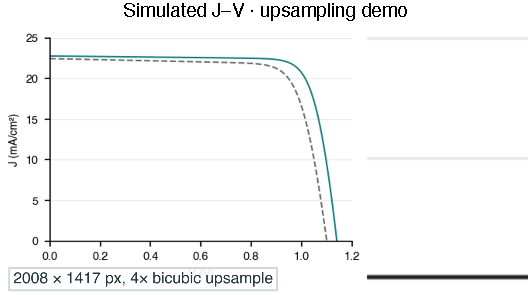
\includegraphics[width=85mm]{figures/ch13/ch13-02a-upsampled-en.pdf}\\[1.5mm]
{\footnotesize (a) Rendered at $150\ \text{dpi}$ ($502 \times 354\ \text{px}$), then enlarged $4\times$ by bicubic interpolation to $2008 \times 1417\ \text{px}$}\\[3mm]
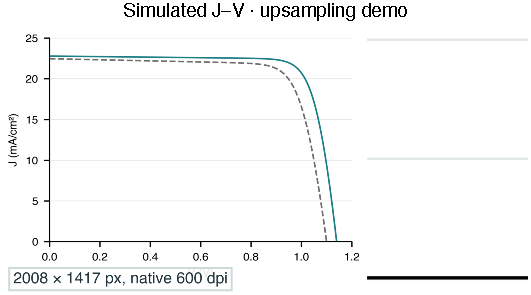
\includegraphics[width=85mm]{figures/ch13/ch13-02b-native-en.pdf}\\[1.5mm]
{\footnotesize (b) Rendered directly at $600\ \text{dpi}$ ($2008 \times 1417\ \text{px}$)}
\caption{Same pixel count, different information. (a) Rendered at 150 dpi, then interpolated to 600 dpi; (b) rendered directly at 600 dpi. Insets are magnified 8$\times$. Simulated data.}\label{fig:ch13-02}
\end{figure}

Compare the two panels of Figure~\ref{fig:ch13-02}. Both files measure $2008 \times 1417\ \text{px}$, so an automated dimension check reports $600\ \text{ppi}$ for both. Yet the visual difference is unmistakable. In the full plot on the left of Figure~\ref{fig:ch13-02}a, the tick numerals (\texttt{0.0}--\texttt{1.2} and \texttt{0}--\texttt{25}), vertical axis title (`\texttt{J (mA/cm\textsuperscript{2})}'), and curves look blurry. On the right, the $8\times$ inset crops the bottom black axis spine and two light-grey horizontal grid lines: in Figure~\ref{fig:ch13-02}a, both the axis spine and grid lines carry fuzzy grey halos along their upper and lower edges---the smear left behind when a $502 \times 354\ \text{px}$ grid is interpolated $4\times$. In Figure~\ref{fig:ch13-02}b, rendered directly at $600\ \text{dpi}$, every character and line edge stays crisp.

Notice also two layout flaws inside Figure~\ref{fig:ch13-02} itself: first, the bottom-left pixel-count box was placed at a fixed relative coordinate and overlaps the top half of the horizontal axis title `\texttt{V (V)}'; second, the vertical crop window for the $8\times$ inset captured only the flat grid lines and bottom axis rather than the curved $J\text{--}V$ knee and tick text. When you run an $800\%$ zoom check on your own figures, always pan across curve knees, diagonal strokes, and superscripts rather than inspecting only flat horizontal lines.

Mathematical interpolation (bilinear, bicubic, or Lanczos) fills smooth intermediate values between old pixels; \textbf{it increases file size without adding real spatial information}. Even more hazardous is \textbf{generative AI super-resolution upscaling}. Passing a low-resolution scanning electron micrograph (SEM), fluorescence image, or Western blot through an AI upscaler produces sharp-looking edges by hallucinating textures from its training corpus---turning blurry grain boundaries into crisp facets or inventing pores in background noise. As Chapter 8 established, primary experimental images are observational evidence: \textbf{never apply generative AI upscaling or redrawing to scientific evidence images}. If an experimental panel lacks effective resolution, either re-export the full-resolution master from the instrument or reduce that panel's physical millimetre width in the layout and document its native pixel count in the processing log.

In \scidraw{}, distinguish between two export mechanisms: general image-conversion utilities map nominal dpi choices to fixed maximum pixel side lengths and may invoke AI upscaling when a source image is small, so they must never be used to ``boost dpi'' on experimental micrographs; by contrast, the multi-panel assembly workspace (\sdtool{multi-panel-figure-maker}) calculates canvas dimensions strictly from target physical millimetres and dpi, recording each panel's native pixels, physical width, and effective resolution in \texttt{processing-log}.

\section{Text and line weight at final size}

The second frequent cause of technical returns and reader frustration is \textbf{unintended shrinkage of font sizes and line weights at final print width}.

Many researchers draft plots in Python (Matplotlib), R, Origin, or PowerPoint on a wide default canvas while looking at a large monitor: $10\ \text{pt}$ axis labels look clear on screen, but shrink to near-illegibility when scaled into a narrow journal column. Whenever a wide canvas is scaled down to a narrower target column width, every font size and stroke width scales down by the exact same linear ratio:
\[
\text{Final font size (pt)} = \text{Drafting font size (pt)} \times \frac{\text{Final layout width (mm)}}{\text{Drafting canvas width (mm)}}
\]

Two everyday scenarios show how fast text drops below journal limits:
\begin{itemize}
\item \textbf{Scaling down a wide Matplotlib canvas:} The paired-comparison plot from Chapters 1 and 5 was originally drafted on a $7.3\ \text{in}$ ($185.4\ \text{mm}$) canvas with $10\ \text{pt}$ text. Across a $180\ \text{mm}$ double column, the text prints at $10 \times 180 \div 185.4 \approx 9.7\ \text{pt}$. Placed into an $85\ \text{mm}$ single column (or half of a double-column composite), however, the scaling ratio becomes $85 \div 185.4 \approx 0.458$, shrinking $10\ \text{pt}$ text to $10 \times 85 \div 185.4 \approx 4.6\ \text{pt}$ ($4.58\ \text{pt}$). That falls below Elsevier's $7\ \text{pt}$ target, PLOS ONE's $8\ \text{pt}$ minimum, and even Nature's $5\ \text{pt}$ floor.
\item \textbf{Scaling down a widescreen PowerPoint slide:} A standard 16:9 slide is $33.867\ \text{cm}$ ($338.7\ \text{mm}$) wide. Shrinking a full-slide diagram into an $85\ \text{mm}$ single column scales everything by $85 \div 338.7 \approx 0.251$: $24\ \text{pt}$ headings drop to $6.0\ \text{pt}$, and $18\ \text{pt}$ notes collapse to $4.5\ \text{pt}$.
\end{itemize}

Figure~\ref{fig:ch13-03} prints both approaches for the paired-comparison dataset (8 simulated subjects, where \texttt{SIM04} drops from 18 to 17) at \textbf{actual $85\ \text{mm}$ physical width}, letting you compare $4.6\ \text{pt}$ and $7\ \text{pt}$ directly on the page.

\begin{figure}[htbp]\centering
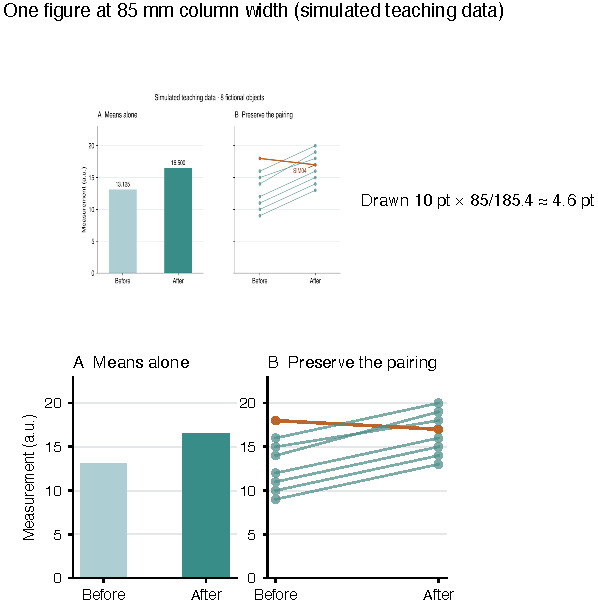
\includegraphics[width=85mm]{figures/ch13/ch13-03-text-at-final-width-en.pdf}
\caption{One figure, two outcomes in an 85 mm column. Top: drawn 7.3 in (185 mm) wide with 10 pt text, which shrinks to about 4.6 pt; bottom: drawn at final width with 7 pt text. Both are printed at actual size. Simulated teaching data.}\label{fig:ch13-03}
\end{figure}

In the top half of Figure~\ref{fig:ch13-03}, shrinking the $185.4\ \text{mm}$ plot into the single-column width reduces the vertical axis title (`\texttt{Measurement (a.u.)}'), bar-top means (`\texttt{13.125}', `\texttt{16.500}'), and subject label `\texttt{SIM04}' to about $4.6\ \text{pt}$, while thinning the axis spines and grid lines until they look faint. In the bottom half, the script set the canvas width directly to $85\ \text{mm}$, with $7\ \text{pt}$ ticks and axis labels, $8\ \text{pt}$ subplot titles (`\texttt{A Means alone}', `\texttt{B Preserve the pairing}'), $0.75\ \text{pt}$ paired lines, $1.2\ \text{pt}$ for \texttt{SIM04}, and no cluttered three-decimal bar labels. Every label reads cleanly.

Figure~\ref{fig:ch13-03} also illustrates a real layering pitfall from script assembly: the script placed a margin note at $x = 0.76$ in both rows---`\texttt{Drawn 10 pt $\times$ 85/185.4 $\approx$ 4.6 pt}' in the top row and `\texttt{Final 7 pt}' in the bottom row. Because the bottom row's two subplots span the full $85\ \text{mm}$ width out to $x = 0.98$, their white subplot canvas covered up the `\texttt{Final 7 pt}' note underneath. Always inspect the rendered page visually after combining subplots or overlays.

Line weights scale by the same ratio: a $0.5\ \text{pt}$ line on a $185\ \text{mm}$ canvas thins to $0.23\ \text{pt}$ at $85\ \text{mm}$ width, approaching the lower limit of journal rules (Elsevier specifies $0.10\text{--}1.5\ \text{pt}$) and risking broken hairlines in print.

Two habits prevent font and line-weight shrinkage:
\begin{enumerate}
\item \textbf{Set the canvas to final millimetre dimensions from the start (scale factor 1.0):} Use $\texttt{figsize}=(85/25.4,\ H/25.4)$ (or $89\ \text{mm}$ / $90\ \text{mm}$) for single-column plots and $(174/25.4,\ H/25.4)$ (or $183\ \text{mm}$ / $190\ \text{mm}$) for double-column plots so that $7\ \text{pt}$ in code prints as $7\ \text{pt}$ on paper.
\item \textbf{Print a 100\% paper proof and measure with a ruler:} Place the figure at its target millimetre width on an A4/Letter page, print at 100\% scale, check the frame width with a ruler, and measure uppercase letter height. Since $1\ \text{pt} = 1/72\ \text{in} \approx 0.353\ \text{mm}$ and sans-serif uppercase cap height is about $0.7\times$ point size, final $7\ \text{pt}$ capitals measure roughly $1.7\text{--}1.8\ \text{mm}$ tall ($8\ \text{pt} \approx 2.0\ \text{mm}$). If capitals measure under $1.2\ \text{mm}$, an unintended rescaling step occurred.
\end{enumerate}

\section{Vector, raster and container formats}

Why did the journal's preflight system reject Zhou's Figure 2 PDF as a ``low-resolution bitmap''? Because he equated a \textbf{file extension} with \textbf{what is stored inside the file}.

Graphics files fall into three structural categories (Figure~\ref{fig:ch13-04}):
\begin{itemize}
\item \textbf{Pure raster files (PNG, TIFF, JPEG):} Store a 2D pixel grid. At $800\%$ zoom, curves and letters break into square pixels. Raster formats suit photographs, micrographs, gels, and text-free generated base illustrations.
\item \textbf{True vector content (PDF, SVG, or EPS with paths and live text):} Store mathematical coordinates for lines, B\'{e}zier curves, fills, and character strings linked to embedded fonts. Edges remain sharp at any magnification, and axis labels can be selected as live text.
\item \textbf{``Container'' files (PDF, SVG, EPS, or PPTX wrapping a bitmap):} PDF, SVG, EPS, and PPTX are \textbf{compound containers}. They can hold vector paths and fonts, or they can simply wrap a single PNG/JPEG bitmap. Saving a $150\ \text{dpi}$ PNG as a PDF produces a \texttt{.pdf} file whose content is still a $150\ \text{ppi}$ bitmap.
\end{itemize}

\begin{figure}[htbp]\centering
\resizebox{\linewidth}{!}{% FIG ch13-04 what's inside the file (English)
\usetikzlibrary{arrows.meta,positioning,fit}
\begin{tikzpicture}[
  font=\sffamily\footnotesize, text=BookInk,
  card/.style={draw=BookRule, line width=0.6pt, rounded corners=3pt,
    fill=BookPale!30, minimum width=42mm, minimum height=38mm, align=center, inner sep=5pt},
]
  \node[card] (C1) at (0,0) {%
    \textbf{Raster files}\\PNG, TIFF, JPEG\\[4pt]
    \tikz{\foreach \x in {0,1,2,3} \foreach \y in {0,1,2,3}
      \fill[BookTeal!35] (\x*0.35,\y*0.35) rectangle ++(0.32,0.32);}\\[3pt]
    \scriptsize Zoom in to see pixels;\\photos and micrographs};
  \node[card, right=6mm of C1] (C2) {%
    \textbf{Vector content}\\paths and text inside PDF/SVG/EPS\\[4pt]
    \tikz{\draw[BookTeal, line width=0.8pt] (0,0.6) .. controls (0.5,1.2) and (1.2,0.2) .. (1.6,0.8);
      \node[font=\sffamily] at (0.8,0.2) {Aa};}\\[3pt]
    \scriptsize Edges stay sharp;\\selectable text, embedded fonts};
  \node[card, right=6mm of C2] (C3) {%
    \textbf{Container}\\vector-like name, bitmap inside\\[4pt]
    \tikz{\draw[BookRule, fill=white] (-0.1,-0.1) rectangle (1.7,1.3);
      \foreach \x in {0,1,2} \foreach \y in {0,1,2}
        \fill[BookInk!25] (0.2+\x*0.35,0.2+\y*0.28) rectangle ++(0.3,0.24);}\\[3pt]
    \scriptsize PDF/SVG/EPS/PPTX\\may wrap a single bitmap};

  \node[draw=BookTeal, fill=white, rounded corners=2pt, inner sep=5pt,
    text width=132mm, align=left, font=\scriptsize, below=8mm of C2] (how) {%
    \textbf{How to check:}\ 
    \texttt{pdffonts}, \texttt{pdfimages -list}, 800\,\% zoom,
    search SVG for \texttt{<image}, unzip PPTX \texttt{ppt/media/}.};

  \node[draw=BookRule, fill=BookPale!15, rounded corners=2pt, inner sep=4pt,
    text width=132mm, align=left, font=\scriptsize, below=3mm of how] {%
    \textbf{SciDraw AI exports to note:}
    declarative chart PDF/EPS is raster-wrapped;
    image-to-SVG text mode keeps a bitmap background;
    image-to-PPTX is background + OCR boxes;
    multi-panel PPTX uses bitmap panels and text labels.};
\end{tikzpicture}
}
\caption{The file extension does not tell you what is inside. PDF, SVG, EPS and PPTX can hold vector objects or just wrap a bitmap.}\label{fig:ch13-04}
\end{figure}

Five practical checks reveal whether a container holds true vector objects or a wrapped bitmap:

\begin{enumerate}
\item \textbf{Check embedded fonts with \texttt{pdffonts} (command line):} The Poppler utility \texttt{pdffonts} lists all fonts in a PDF and whether they are embedded (\texttt{emb=yes}) and subsetted (\texttt{sub=yes}). If a figure displays visible text yet \texttt{pdffonts} outputs nothing, the text has either been rasterized into pixels or converted into uneditable outline paths. Note that journals such as Nature explicitly instruct authors neither to rasterize line art/text nor to outline text.
\item \textbf{List internal bitmaps with \texttt{pdfimages -list} (command line):} This command reports every raster image inside a PDF, including pixel dimensions, colour space, and effective \texttt{x-ppi}/\texttt{y-ppi}. If a standalone line chart appears as a full-page bitmap in \texttt{pdfimages -list}, it is a raster container. Conversely, in a multi-panel PDF like Chapter 9's Figure 2 (schematic bitmaps in \textbf{a}, \textbf{b}; data plots in \textbf{c}, \textbf{d}), \texttt{pdfimages -list} \textbf{should list only panels a and b}, while panels \textbf{c} and \textbf{d} stay pure vector. Photographs and generated bases are naturally raster; plotted curves and text must stay vector.
\item \textbf{Zoom to 800\% and select text in a PDF viewer (no command line):} Try highlighting axis labels with the text cursor, then zoom to $800\%$ to see whether curves stay smooth or break into pixel stairs (or use Adobe Acrobat Pro's ``Preflight'' object inspector).
\item \textbf{Search SVG files in a text editor:} Open the \texttt{.svg} file and search for \texttt{<image}. A file containing only a Base64 PNG string is a bitmap wrapper; a true vector SVG contains hundreds of \texttt{<path>}, \texttt{<line>}, and \texttt{<text>} tags.
\item \textbf{Unzip PPTX files:} Copy \texttt{.pptx} to \texttt{.zip}, extract it, and inspect \texttt{ppt/media/} to see every embedded bitmap.
\end{enumerate}

Figure~\ref{fig:ch13-05} and Table~\ref{tab:ch13-02} compare a true vector PDF (\texttt{vector.pdf}, with \texttt{pdf.fonttype = 42}) and a $150\ \text{ppi}$ bitmap-container PDF (\texttt{container.pdf}) generated from the same simulated perovskite $J\text{--}V$ data\allowbreak{} ($85 \times 60\ \text{mm}$).

\begin{figure}[htbp]\centering
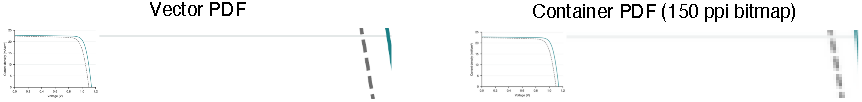
\includegraphics[width=\linewidth]{figures/ch13/ch13-05-vector-vs-container-en.pdf}
\caption{Both are PDFs. Left: vector paths and embedded fonts stay sharp when magnified; right: a wrapped 150 ppi bitmap shows its pixels. Simulated data.}\label{fig:ch13-05}
\end{figure}

\begin{table}[htbp]\centering\footnotesize
\setlength{\tabcolsep}{4pt}
\renewcommand{\arraystretch}{1.18}
\caption{Measured output from running \texttt{pdffonts} and \texttt{pdfimages -list} on the two PDF files in Figure~\ref{fig:ch13-05}.}\label{tab:ch13-02}
\begin{tabularx}{\linewidth}{@{}>{\raggedright\arraybackslash}p{26mm}>{\raggedright\arraybackslash}p{23mm}Y@{}}
\toprule
\textbf{File and nature} & \textbf{Command} & \textbf{Measured output summary and interpretation} \\
\midrule
\texttt{vector.pdf} (true vector PDF) & \texttt{pdffonts} & Lists \texttt{Helvetica} (\texttt{CID TrueType}) with \texttt{emb=yes}, \texttt{sub=yes} (plus \texttt{FandolHei-Regular} in the Chinese build), confirming embedded font subsets \\
\texttt{vector.pdf} (true vector PDF) & \texttt{pdfimages -list} & No entries (empty output), proving axes, grid lines, and both curves are pure vector paths \\
\texttt{container.pdf} (bitmap container) & \texttt{pdffonts} & No entries (empty output), proving visible axis labels are no longer text objects \\
\texttt{container.pdf} (bitmap container) & \texttt{pdfimages -list} & Lists 1 RGB bitmap on page 1 ($502 \times 355\ \text{px}$, \texttt{x-ppi=150} when wrapped directly; or degraded to $260 \times 182\ \text{px}$, \texttt{x-ppi=100} if re-saved via Matplotlib \texttt{imshow} at default \texttt{savefig.dpi=100}) \\
\bottomrule
\end{tabularx}
\end{table}

Alongside the sharp vector inset on the left and the pixelated bitmap inset on the right of Figure~\ref{fig:ch13-05}, this test highlights two subtle traps in real workflows:

First is the \textbf{missing-glyph trap in embedded fonts}. In Figure~\ref{fig:ch13-05}, the English y-axis label `\texttt{Current density (mA/cm\textsuperscript{2})}' uses Helvetica, which contains the Unicode superscript two (`\texttt{\textsuperscript{2}}', \texttt{U+00B2}). When the same script assigns the entire label to a font lacking \texttt{U+00B2}---as occurred in the Chinese build with \texttt{FandolHei-Regular.otf}, or when a specialty font lacks $\mu$ or minus signs---\texttt{pdffonts} still reports \texttt{emb=yes}, yet the superscript silently disappears into a blank space in the vector PDF and turns into a missing-glyph box (`tofu') in the container PDF. Always pair \texttt{pdffonts} with an $800\%$ visual check, and render scientific units via math mode (\texttt{\$\textbackslash mathrm\{mA\textbackslash,cm\textasciicircum\{-2\}\}\$}) or a verified Latin/symbol font.

Second is \textbf{silent downsampling during secondary wrapping}. As noted in Table~\ref{tab:ch13-02}, placing a $150\ \text{dpi}$ bitmap ($502 \times 354\ \text{px}$) into a new Matplotlib figure via \texttt{imshow} and calling \texttt{savefig("container.pdf")} without a \texttt{dpi} argument resamples the image at the default \texttt{savefig.dpi = 100}, shrinking it to $260 \times 182\ \text{px}$ ($100\ \text{ppi}$). Running \texttt{pdfimages -list} catches this immediately.

Keep in mind the actual internal structure of exports from current \scidraw{} modules:
\begin{itemize}
\item \textbf{Scientific visualization (\sdtool{sci-vis}):} PDF and EPS files exported from its declarative chart pathway are \textbf{raster-wrapped containers}. When a journal requires true vector data plots with embedded fonts, download the verified data table from \sdtool{sci-vis} and run a deterministic script (\texttt{pdf.fonttype = 42}) at final physical dimensions.
\item \textbf{Image-to-SVG and image-to-PPTX:} Converting a bitmap to SVG in text-layer mode retains a bitmap background underneath; converting to PPTX yields a background bitmap plus OCR text boxes rather than semantic vector objects.
\item \textbf{Multi-panel assembly (\sdtool{multi-panel-figure-maker}):} In exported PPTX files, panels are bitmaps and panel letters (\textbf{a}--\textbf{d}) are editable text boxes; curves inside panels cannot be ungrouped in PowerPoint.
\end{itemize}

\section{Colour: RGB/CMYK, grayscale and colour-vision deficiency}

Colour inspection answers three questions: Which colour space should you submit? Can groups be told apart in black-and-white printouts? And does the figure work for readers with colour-vision deficiency (CVD)?

\subsection*{RGB versus CMYK: keep an sRGB master and do not convert blindly}

Screens mix red, green, and blue light (additive RGB, wide gamut), whereas printing presses layer cyan, magenta, yellow, and black inks (subtractive CMYK, narrower gamut, especially in bright greens and cyans).

Older tutorials often advised converting all figures to CMYK before submission. Today, most scientific reading happens online in HTML and PDF, and the three official publisher guidelines verified for this chapter (as of 29 October 2026) all recommend or accept RGB:
\begin{itemize}
\item \textbf{Nature:} Recommends submitting RGB artwork; production converts RGB to CMYK for print while keeping vivid RGB originals in online HTML and PDF editions.
\item \textbf{Elsevier:} Explicitly states ``RGB preferred.''
\item \textbf{PLOS ONE:} Requires $8\ \text{bit}$/channel RGB or grayscale.
\end{itemize}

Converting to CMYK locally with an arbitrary ICC profile dulls colours for online readers and risks a second colour shift on press. \textbf{Always retain and submit an RGB master with an embedded sRGB profile; convert a copy to CMYK only when a journal explicitly mandates it, and inspect saturated hues after conversion.}

\subsection*{Grayscale legibility: check perceptual lightness $L^*$, not the RGB average}

When Zhou's collaborator asked which curve was the control on her monochrome printout, she uncovered a real issue left in our Chapter 9 and Chapter 12 drafts.

In Chapter 12, we paired dark grey (\texttt{\#6E6E6E}, control) with deep teal (\texttt{\#1B7F86}, modified). On a colour monitor, their perceptual colour difference (CAM02-UCS $\Delta E$) is $19.8$. In grayscale, however, human brightness perception does not average $(R + G + B)/3$; it follows spectral sensitivity captured by \textbf{relative luminance ($Y$) and CIE 1976 perceptual lightness ($L^*$)}. After linearizing gamma-encoded sRGB channels into $(R_{\text{lin}}, G_{\text{lin}}, B_{\text{lin}})$, Rec.~709 luminance is:
\[
Y = 0.2126\,R_{\text{lin}} + 0.7152\,G_{\text{lin}} + 0.0722\,B_{\text{lin}}
\]
Mapping $Y$ to CIE $L^* \in [0, 100]$ for our case colours yields:
\begin{itemize}
\item Control dark grey \texttt{\#6E6E6E} ($\text{RGB} = 110, 110, 110$): \textbf{$L^* = 46.4$};
\item Modified deep teal \texttt{\#1B7F86} ($\text{RGB} = 27, 127, 134$): because red is near zero, \textbf{$L^* = 48.4$};
\item Draft red \texttt{\#CC0000} ($\text{RGB} = 204, 0, 0$): $L^* = 42.5$;
\item Draft green \texttt{\#2CA02C} ($\text{RGB} = 44, 160, 44$): $L^* = 57.9$.
\end{itemize}

The calculation explains the printout failure immediately: \textbf{control grey ($L^* = 46.4$) and modified teal ($L^* = 48.4$) differ by only $2.0$ lightness units, collapsing their grayscale difference to $\Delta E = 2.1$!} Two solid lines at $L^* = 46.4$ and $48.4$ look identical on paper. Every figure needs a true $L^*$ grayscale check.

\subsection*{Colour-vision deficiency simulation and redundant encoding}

Human trichromatic vision uses long- ($L$, red-sensitive), middle- ($M$, green-sensitive), and short-wavelength ($S$, blue-sensitive) retinal cones. Inherited CVD falls into three classes:
\begin{enumerate}
\item \textbf{Protan ($L$-cone alteration):} Protanomaly and protanopia; reds and greens confuse, and pure reds appear darkened.
\item \textbf{Deutan ($M$-cone alteration):} Deuteranomaly and deuteranopia; the most common type, collapsing reds and greens into similar olive-brown tones.
\item \textbf{Tritan ($S$-cone alteration):} Tritanomaly and tritanopia; rarer, affecting blue--green and yellow--violet pairs.
\end{enumerate}

As Wong (2011) noted, roughly $8\%$ of men (and about $0.5\%$ of women) of Northern European ancestry have red--green CVD. Crameri, Shephard, and Heron (2020) further showed that rainbow colormaps (such as Jet) both fail CVD readers and distort data gradients due to uneven $L^*$ profiles.

To simulate CVD computationally, Brettel, Vi\'{e}not, and Mollon (1997) projected colours in LMS cone space for dichromacy, while Machado, Oliveira, and Fernandes (2009) modelled spectral shifts across severities $0\text{--}100$ using $3 \times 3$ matrices in \textbf{linear RGB space}. Figure~\ref{fig:ch13-06} applies the Machado et al.\ (2009) model at $\text{severity} = 100$ (via \texttt{colorspacious} v1.1.2, verified against the original paper's matrices) across three palette rows and five views, printing the CAM02-UCS $\Delta E$ between the two curves in the upper-right corner of each cell.

\begin{figure}[htbp]\centering
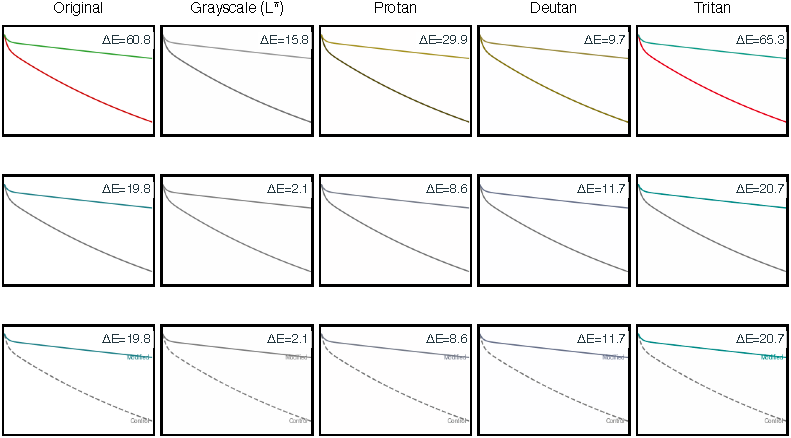
\includegraphics[width=\linewidth]{figures/ch13/ch13-06-grayscale-and-cvd-en.pdf}
\caption{Three colour schemes for one plot, seen in grayscale and under simulated colour-vision deficiencies. Row 2 (the Chapter 12 colours) is almost indistinguishable in grayscale; row 3 adds a line style and stays distinguishable in every view. Simulations use the Machado et al. (2009) model at full severity and are approximations. Simulated data.}\label{fig:ch13-06}
\end{figure}

Inspecting Figure~\ref{fig:ch13-06} row by row shows:
\begin{itemize}
\item \textbf{Row 1 (solid red \texttt{\#CC0000} and solid green \texttt{\#2CA02C}):} Strong contrast in Original ($\Delta E = 60.8$) and Tritan ($\Delta E = 65.3$), and moderate grayscale separation ($\Delta E = 15.8$ from $L^* = 42.5$ vs.\ $57.9$), but under Deutan (column 4) both curves become murky olive-brown ($\Delta E = 9.7$), inviting mix-ups when matched against a legend box.
\item \textbf{Row 2 (Chapter 12 initial palette: solid grey \texttt{\#6E6E6E} and solid teal \texttt{\#1B7F86}):} Preserves chromatic contrast in Protan ($\Delta E = 8.6$), Deutan ($\Delta E = 11.7$), and Tritan ($\Delta E = 20.7$), but collapses in CIE $L^*$ Grayscale (column 2) to \textbf{$\Delta E = 2.1$}.
\item \textbf{Row 3 (revised: dashed grey \texttt{\#6E6E6E} control, solid teal \texttt{\#1B7F86} modified, plus direct labels `\texttt{Modified}' and `\texttt{Control}'):} The colour $\Delta E$ values ($19.8$, $2.1$, $8.6$, $11.7$, $20.7$) are identical to Row 2 because the hex colours did not change, yet adding \textbf{line style (dashed vs.\ solid)} and \textbf{direct endpoint labels} makes the two groups instantly distinguishable across all five columns.
\end{itemize}

Notice one typographic detail in Row 3 of Figure~\ref{fig:ch13-06}: in these small thumbnails, the $5\ \text{pt}$ labels `\texttt{Modified}' and `\texttt{Control}' were vertically centred right on the $t = 980\ \text{h}$ curve endpoints, so the curve strokes pass through the middle of the words. In full-sized publication finals, offset direct labels slightly above, below, or beside the curve end so lines never strike through text.

Remember two limits of CVD simulations: first, simulations are mathematical approximations for a standard display and observer, not an absolute certification; second, as Machado et al.\ (2009) noted, empirical data for tritan defects are sparser, making tritan simulation less reliable than protan/deutan. The robust solution is \textbf{redundant encoding}: always combine colour with distinct line styles, marker shapes, or direct labels.

\section{Technical checks with \sdtool{figure-checker}}

You can automate bitmap preflight checks using the figure checker in \scidraw{} (\sdtool{figure-checker}). Upload a PNG, JPEG, WebP, or TIFF, select the \textbf{figure type} (\textit{Photograph}, \textit{Combination}, or \textit{Line art}), and choose the \textbf{target layout width} (preset $85\ \text{mm}$ single column, $180\ \text{mm}$ double column, or \textit{Custom width} in millimetres). The tool reports six items with visual previews: (1) \textbf{effective resolution} ($\ge 300\ \text{ppi}$ photo, $\ge 600\ \text{ppi}$ combination, $\ge 900\ \text{ppi}$ line art for ``Pass''), (2) \textbf{format}, (3) \textbf{alpha transparency channel}, (4) \textbf{colour space}, (5) \textbf{grayscale luminance levels and preview}, and (6) \textbf{CVD cluster-collapse check and previews}.

Keep five boundaries in mind and \textbf{never treat a ``Pass'' badge as full journal compliance}:
\begin{enumerate}
\item \textbf{Technical screening, not scientific review:} It does not verify statistics, error-bar definitions, data honesty, or journal policies.
\item \textbf{Default $180\ \text{mm}$ double column differs from specific journals:} Nature uses $183\ \text{mm}$, Springer/Cell $174\ \text{mm}$, Elsevier $190\ \text{mm}$, and individual subpanels may be $69\ \text{mm}$ or $92\ \text{mm}$. Always use \textbf{Custom width}.
\item \textbf{It does not check font size, line weight, or PDF vector structure:} A $600\ \text{dpi}$ PNG with $4.5\ \text{pt}$ text still passes resolution. Check typography per Section 13.2 and PDF internals per Section 13.3.
\item \textbf{Tool thresholds are general defaults:} The checker passes line art at $\ge 900\ \text{ppi}$, whereas Elsevier requires $1000\ \text{dpi}$ ($1200\ \text{dpi}$ for fine lines). Target journal rules always govern.
\item \textbf{Automated grayscale/CVD flags do not replace visual inspection:} Global luminance level counts include black axes and white backgrounds and may not flag two curves with similar $L^*$ values; always inspect the grayscale and CVD preview images directly.
\end{enumerate}

\section{Journal requirements: check the current official page}

Table~\ref{tab:ch13-01} summarizes three official artwork guideline pages verified directly on \textbf{29 October 2026}: Nature (\textit{Guide to preparing final artwork}), PLOS ONE (\textit{Figures}), and Elsevier (\textit{Artwork sizing} and \textit{Artwork types}).

\begin{table}[htbp]\centering\footnotesize
\setlength{\tabcolsep}{3pt}
\renewcommand{\arraystretch}{1.18}
\caption{Official technical artwork requirements across three publishers/journals (verified 29 October 2026; re-verify the live official page before submission).}\label{tab:ch13-01}
\begin{tabularx}{\linewidth}{@{}>{\raggedright\arraybackslash}p{20mm}YYY@{}}
\toprule
\textbf{Item} & \textbf{Nature (\textit{Guide to preparing final artwork})} & \textbf{PLOS ONE (\textit{Figures})} & \textbf{Elsevier (\textit{Artwork sizing / types})} \\
\midrule
Widths & Single $89\ \text{mm}$; double $183\ \text{mm}$; $1.5$-col $120$ or $136\ \text{mm}$ & $6.68\text{--}19.05\ \text{cm}$ ($789\text{--}2250\ \text{px}$ at $300\ \text{dpi}$) & Min $30\ \text{mm}$; single $90\ \text{mm}$; $1.5$-col $140\ \text{mm}$; double $190\ \text{mm}$ \\
Max height & $247\ \text{mm}$ & $22.23\ \text{cm}$ ($2625\ \text{px}$ at $300\ \text{dpi}$) & Not listed separately on these pages \\
Resolution & Photos $\ge 300\ \text{dpi}$ at print size; do not rasterize line art/text & $300\text{--}600\ \text{dpi}$ & Photos $300\ \text{dpi}$; combo $500\ \text{dpi}$; line art $1000\ \text{dpi}$ (fine $1200\ \text{dpi}$) \\
Formats & AI, vector EPS, PSD, PS, PDF, PPT, Word, Excel, CorelDraw ($\le \text{v8}$); convert JPEG/TIFF/PNG to PDF/EPS/PS & TIFF or EPS & Line art: EPS or TIFF; photos/combo: TIFF or top-quality JPEG; Office accepted as hybrid vector \\
Colour & RGB recommended (auto-converted to CMYK for print; RGB kept online) & RGB ($8\ \text{bit}$/ch) or grayscale & RGB preferred \\
Fonts \& size & Sans-serif (Helvetica/Arial); panel letters $8\ \text{pt}$ bold lowercase; other text $5\text{--}7\ \text{pt}$; do not outline & Arial, Times, or Symbol, $8\text{--}12\ \text{pt}$ & Embed fonts; preferred Arial/Helvetica, Courier, Times, Symbol; final body $7\ \text{pt}$, scripts $\ge 6\ \text{pt}$ \\
Other & --- & $< 10\ \text{MB}$; flatten TIFF, no alpha, LZW; NAAS precheck advised & Line weights $0.10\text{--}1.5\ \text{pt}$ \\
\bottomrule
\end{tabularx}
\end{table}

Three practical rules follow from Table~\ref{tab:ch13-01}:
\begin{enumerate}
\item \textbf{Different journals have conflicting rules:} Nature caps body labels at $7\ \text{pt}$ ($5\text{--}7\ \text{pt}$), whereas PLOS ONE requires $8\text{--}12\ \text{pt}$. Switching journals requires re-running your plotting script with updated parameters.
\item \textbf{Two official guides from the same publisher can differ:} Nature's final artwork guide specifies $89 / 183\ \text{mm}$, whereas another Nature Portfolio guide lists $88 / 180\ \text{mm}$. While \scidraw{}'s multi-panel presets cite their source URLs, always check your specific journal's live page.
\item \textbf{Record the official URL and access date in your brief and README:} If an AI assistant summarizes a guideline page for you, verify every number against the original page yourself.
\end{enumerate}

\section{A traceable delivery package}

Finally, organize all materials into a \textbf{delivery package that a colleague can understand and reproduce without asking you}. Following the FAIR principles (Wilkinson et al., 2016) and reproducible research rules (Sandve et al., 2013), Figure~\ref{fig:ch13-08} shows a standard directory tree.

\begin{figure}[htbp]\centering
{\let\tag\undefined\makeatletter\tikzset{below/.code=\tikz@lib@place@handle@{#1}{north west}{0}{-1}{south west}{1}}\makeatother% FIG ch13-08 delivery package tree (English)
\usetikzlibrary{positioning}
\providecommand{\ChThirteenMarkTool}{\tikz[baseline=-0.55ex]{\fill[BookInk] (0,0) rectangle (1.5mm,1.5mm);}}
\providecommand{\ChThirteenMarkSelf}{\tikz[baseline=-0.55ex]{\draw[BookInk, line width=0.35pt] (0,0) rectangle (1.5mm,1.5mm);}}
\providecommand{\tag}[1]{{\tiny\color{BookInk!75}#1}}
\noindent
\begin{tikzpicture}[
  font=\sffamily\scriptsize, text=BookInk,
  folder/.style={anchor=west, align=left},
  tagline/.style={font=\tiny, text=BookInk!75, align=left},
]
  \node[folder] (root) at (0,0) {perovskite-fig2\_\\delivery\_\\2026-10-29/};
  \node[folder, below=2mm of root.south west, xshift=4mm] (readme) {README.md};
  \node[tagline, below=0.5mm of readme.south west] (readmetag) {what\\it is,\\how to reproduce,\\contact};
  \node[folder, below=1.5mm of readmetag.south west, xshift=4mm] (b0) {00\_brief/\\[-2pt]\tag{briefs,}\\[-1pt]\tag{journal excerpts}};
  \node[folder, below=1.5mm of b0.south west, xshift=4mm] (s1) {01\_source/ \ChThirteenMarkSelf\ raw images\\[-2pt]\& CSV \tag{not in tool}\\[-1pt]\tag{ZIP}};
  \node[folder, below=1.5mm of s1.south west, xshift=4mm] (s1d) {data/ · images/};
  \node[folder, below=1.5mm of s1d.south west] (c2) {02\_code/ \ChThirteenMarkSelf\ scripts\\[-2pt]\& environment};
  \node[folder, below=1.5mm of c2.south west, xshift=4mm] (d3) {03\_drafts/ \ChThirteenMarkSelf\ v01–v04\\[-2pt]\& instructions};
  \node[folder, below=1.5mm of d3.south west, xshift=4mm] (f4) {04\_final/ \ChThirteenMarkTool\ paper / talk /\\poster};
  \node[folder, below=1.5mm of f4.south west, xshift=4mm] (f4p) {paper/ · talk/ · poster/};
  \node[folder, below=1.5mm of f4p.south west] (r5) {05\_records/};
  \node[folder, below=1.5mm of r5.south west, xshift=4mm] (r5a) {ai-use-log.md \ChThirteenMarkSelf};
  \node[folder, below=1mm of r5a.south west] (r5b) {processing-log.md \ChThirteenMarkSelf};
  \node[folder, below=1mm of r5b.south west] (r5c) {checks/ \ChThirteenMarkTool\ checker reports\\[-2pt]\& CLI output};
  \node[folder, below=1mm of r5c.south west] (r5d) {multi-panel-export/ \ChThirteenMarkTool\ multi-panel\\ZIP};

  \draw[BookInk!40, thin] (root.south west) ++(0,-1mm) coordinate (rt) -- (readme.west |- rt) -- (readme.west);
  \foreach \a/\b in {readmetag/b0,b0/s1,s1/s1d,s1d/c2,c2/d3,d3/f4,f4/f4p,f4p/r5,r5/r5a,r5a/r5b,r5b/r5c,r5c/r5d} {
    \draw[BookInk!30, thin] (\a.south west) ++(0,-0.5mm) coordinate (st) -- (\b.west |- st) -- (\b.west);
  }

  \node[tagline, anchor=north west] at ([yshift=-3mm]r5d.south-|root.west) {%
    \ChThirteenMarkTool\ Tool export:\\ZIP, data\\download,\\checker report\\[2pt]
    \ChThirteenMarkSelf\ Author\\must keep:\\raw images,\\scripts, briefs, AI\\log\\[4pt]
    README: What\\is this?\\How to\\reproduce?\\Which AI steps\\and how verified?};
\end{tikzpicture}
}
\caption{A delivery package a colleague can take over. Filled squares mark content a tool can export; open squares mark material the author must keep separately.}\label{fig:ch13-08}
\end{figure}

Figure~\ref{fig:ch13-08} uses filled squares and open squares to distinguish tool exports from author-archived materials because of two platform boundaries:
\begin{itemize}
\item \textbf{Multi-panel ZIP exports exclude raw panel images and reloadable layouts:} The ZIP from \sdtool{multi-panel-figure-maker} contains final TIFF, PNG, PDF, PPTX files and \texttt{processing-log}, \textbf{not uncropped source images or a cross-computer layout file} (the workspace lives in browser local storage). Save raw images in \texttt{01\_source/images/}.
\item \textbf{Data plots log source integrity, but scripts must be saved in \texttt{02\_code/}:} \sdtool{sci-vis} records the source table's hash, byte size, and row count and lets you download the data, but plotting code is not downloadable from the UI; archive reproduction scripts in \texttt{02\_code/}.
\end{itemize}

Use a four-part filename rule across the package: \path{<project>_<figure-or-venue>_<content>_v<2-digit-version>[_<lang>].<ext>} (e.g., \texttt{perovskite\_\allowbreak fig2c\_\allowbreak jv\_\allowbreak v05\_en.pdf}). Follow three rules: (1) lowercase ASCII, digits, hyphens, and underscores only; (2) increment version numbers monotonically (\texttt{v01}, \texttt{v02}\dots) and never use \texttt{final}; (3) state which version was submitted in the root \texttt{README.md}.

Inside \texttt{05\_records/}, store the \textbf{AI-use log (\texttt{ai-use-log.md})} and \textbf{processing log (\texttt{processing-log.md})}:

\begin{Prompt}
# AI-use log
Project: perovskite-passivation   Figure/Venue: Figure 2 / Slides / Poster   Author: Zhou
| Date | Tool & module | Input (version / rows / hash) | Prompt or instruction path | Output file (version) | Adopted? | Human verification & edits |
|---|---|---|---|---|---|---|
| 2026-10-29 | /ai-drawing | Brief v1 (panel a) | 03_drafts/v01/m1_prompt.txt | m1_base_v02.png | Base adopted | Verified 7-layer order; overlaid 7 pt vector labels |
| 2026-10-29 | /ai-drawing | Brief v1 (panel b) | 03_drafts/v01/m2_prompt.txt | m2_sem_v01.png | Base adopted | Confirmed no fake scale bar; added in-panel model note |
| 2026-10-29 | /sci-vis | metrics.csv (2 rows) | 03_drafts/v04/jv_instr.txt | fig2c_jv_v04.png | Partial | Verified PCE matches CSV; redrew true vector PDF (v05) |
## Stages not using AI
Data simulation and metrics were computed by 02_code/sim_perovskite.py; legend conditions were written by the author.
## Evidential status of generated imagery
M1 is a stack schematic (marked "not to scale"); M2 is a model-generated cross-section illustration, not a micrograph (labelled in-panel across all venues).
## Journal AI policy
Policy URL & date: Elsevier AI author policy (2026-10-29)   Disclosure needed: Complete per target journal instructions.
\end{Prompt}

The companion \texttt{processing-log.md} records simulation parameters, script versions, confirmation of zero data filtering, crop/scaling ratios for \texttt{M1} and \texttt{M2} (referencing the multi-panel log), and the P3 grayscale reason for switching the control curve to a dashed line.

\section{Worked case: delivering Figure 2 and its derivatives}

We now walk through Zhou's delivery workflow for manuscript Figure 2 (targeting Elsevier's general artwork rules), the 3-slide talk deck, and the A0 poster.

\textbf{Step 1: Delivery brief} (\texttt{00\_brief/delivery-brief.txt}).

\begin{Prompt}
[Deliverables] Manuscript Figure 2 (4 panels); talk slides 1--3; A0 poster.
[Target journal rules, accessed 2026-10-29] Elsevier artwork sizing / artwork types pages:
  Double column 190 mm; final body text 7 pt, sub/superscripts >= 6 pt; line weight 0.10--1.5 pt;
  Line art >= 1000 dpi, combination >= 500 dpi, photos >= 300 dpi; RGB preferred; embed fonts.
[Panel nature] a: schematic (bitmap base + vector text); b: model-generated illustration (bitmap); c, d: data plots (true vector).
[Checks] Effective resolution; final font size and line weight; true vector and embedded fonts in c, d;
  group distinguishability in CIE L* grayscale and protan/deutan/tritan views; evidential labels intact.
[Invariants] Data points (control PCE 19.21%, T80 ~210 h; modified PCE 20.98%, 1000 h retention ~86%), axis ranges, group meanings.
[Acceptance] Archive per Figure 13-8; a colleague reading only README.md finds Figure 2c's CSV, script, and instruction within 10 minutes.
\end{Prompt}

\textbf{Step 2: First-round checks on draft \texttt{v04}.} Running CLI checks, font scaling arithmetic, CIE $L^*$ calculation, and \sdtool{figure-checker} reveals four issues (P1--P4) while P5 passes (Table~\ref{tab:ch13-case-round1}).

\begin{table}[htbp]\centering\footnotesize
\setlength{\tabcolsep}{3pt}
\renewcommand{\arraystretch}{1.18}
\caption{First-round delivery check results for Figure 2 and its derivatives (\texttt{v04} draft).}\label{tab:ch13-case-round1}
\begin{tabularx}{\linewidth}{@{}c>{\raggedright\arraybackslash}p{22mm}>{\raggedright\arraybackslash}p{26mm}Y>{\raggedright\arraybackslash}p{16mm}@{}}
\toprule
\textbf{ID} & \textbf{Check item} & \textbf{Method} & \textbf{Measured result and diagnosis} & \textbf{Severity} \\
\midrule
P1 & Vector status of \textbf{c}, \textbf{d} & Run \texttt{pdffonts}, \texttt{pdfimages -list} on PDF from \sdtool{sci-vis} & No font entries, 1 bitmap inside: declarative export is a raster-wrapped container & High \\
P2 & Panel \textbf{a} label font size & Scale panel \textbf{a} source ($7.3\ \text{in}$ wide, $10\ \text{pt}$) into $92\ \text{mm}$ half-column & $10 \times 92 \div 185.4 \approx 5.0\ \text{pt}$, below Elsevier's $7\ \text{pt}$ requirement & High \\
P3 & Grayscale separation & Compute CIE $L^*$: control \texttt{\#6E6E6E} $= 46.4$, modified \texttt{\#1B7F86} $= 48.4$ & Two solid lines have $\Delta E = 2.1$ in grayscale, indistinguishable in monochrome print & Medium \\
P4 & Bitmap effective ppi & Panel \textbf{b} ($1536 \times 1024\ \text{px}$) at $92\ \text{mm}$ width (or $69\ \text{mm}$ in $174\ \text{mm}$ layout) & $1536 \div (92 \div 25.4) \approx 424\ \text{ppi}$ ($565\ \text{ppi}$ at $69\ \text{mm}$); panel \textbf{a} base ($1586 \times 992\ \text{px}$) is $438\ \text{ppi}$ at $92\ \text{mm}$. Meets $\ge 300\ \text{dpi}$ photo rule; log in notes & Low \\
P5 & Evidential labels & Visual inspection across paper, slides, poster & Slides 2--3 and poster state ``Simulated data''; paper \textbf{b}, backup slide, and poster state ``Model-generated illustration, not a micrograph'' & Pass \\
\bottomrule
\end{tabularx}
\end{table}

\textbf{Step 3: Revision instructions (\texttt{v04} $\rightarrow$ \texttt{v05}).}

For \textbf{P1}, querying export capabilities inside \sdtool{sci-vis}:
\begin{Prompt}
Keep all data, axis ranges, colours, and annotations unchanged. I need an editable vector file for journal production:
please state which currently available export formats contain vector paths and editable text.
\end{Prompt}
Confirming that declarative PDF exports are raster containers, Zhou uses the Matplotlib script in \texttt{02\_code/} (\texttt{pdf.fonttype = 42}) to redraw panels \textbf{c} and \textbf{d} as true vector PDFs at final physical dimensions from the same CSV tables, logging in \texttt{processing-log.md}: ``Panels c and d were redrawn by script to obtain vector files; values were verified point-by-point against the \sdtool{sci-vis} version and \texttt{metrics.csv}.''

For \textbf{P2} (updating panel \textbf{a} labels without regenerating the base image):
\begin{Prompt}
Keep the panel a base image (v04) unchanged. In the vector overlay layer, set all layer names to 7 pt (at final 92 mm width)
in Arial/Helvetica (or TeX Gyre Heros) with embedded fonts; keep the correspondence between labels and layers unchanged.
\end{Prompt}

For \textbf{P3} (redundant line-style encoding):
\begin{Prompt}
Keep all data points, axes, and label text unchanged. Change the control group to a dashed line (1.0 pt, #6E6E6E)
and keep the modified group as a solid line (1.0 pt, #1B7F86). Change panel d's 80% reference line to a thin dotted line.
Keep direct curve-end labels and offset them cleanly from the strokes.
\end{Prompt}
This grayscale collision was discovered during this chapter's CIE $L^*$ inspection and propagated back into the final figures of Chapters 9 and 12 so that all chapters match \texttt{v05}.

\textbf{Step 4: Second-round check, final legend, and handoff.} Re-checking \texttt{v05} confirms that the manuscript PDF has all fonts embedded in \texttt{pdffonts} and only panels \textbf{a} and \textbf{b} in \texttt{pdfimages -list} (plus a $7480\ \text{px}$-wide $1000\ \text{dpi}$ LZW RGB TIFF if required by submission portals); talk PNGs are $1920 \times 1080\ \text{px}$; and the A0 poster PDF embeds all fonts with only bitmaps M1 ($2129 \times 1332\ \text{px}$, $150\ \text{ppi}$) and M2 ($1063 \times 709\ \text{px}$, $150\ \text{ppi}$). The updated manuscript legend reads:

\begin{BookNote}
\textbf{Figure 2}\quad Effect of interfacial passivation on simulated device performance and stability (simulated teaching data). (a) Schematic of the n-i-p stack, not to scale. (b) Cross-section, model-generated illustration, not a micrograph. (c) Simulated reverse-scan $J\text{--}V$ curves (single-diode model, AM1.5G, $100\ \text{mW\,cm}^{-2}$); control dashed, modified solid; one representative curve per group. (d) Normalized PCE over time (simulated); the thin dotted line marks 80\% of the initial value (dotted to avoid confusion with the dashed control trace).
\end{BookNote}

Finally, the junior student reads only \texttt{README.md}, locates the CSV data in \texttt{01\_source/\allowbreak data/}, the scripts in \texttt{02\_code/}, and the \texttt{v04} instructions in \texttt{03\_drafts/\allowbreak v04/} within 6 minutes, reruns the script, and confirms that both PCE values ($19.21\%$, $20.98\%$) match \texttt{metrics.csv}.

\section{What AI can and cannot do at this stage}

Table~\ref{tab:ch13-03} summarizes the division of responsibilities during inspection, export, and delivery.

\begin{table}[htbp]\centering\footnotesize
\setlength{\tabcolsep}{3pt}
\renewcommand{\arraystretch}{1.18}
\caption{What AI can do, what AI cannot do, and what the author must check during inspection, export, and delivery.}\label{tab:ch13-03}
\begin{tabularx}{\linewidth}{@{}>{\raggedright\arraybackslash}p{20mm}YYY@{}}
\toprule
\textbf{Stage} & \textbf{What AI can do} & \textbf{What AI cannot do} & \textbf{What the author must check} \\
\midrule
Size \& resolution & \sdtool{figure-checker} computes effective ppi at target width; multi-panel export scales by true dimensions & Restore missing evidence via upscaling; decide whether a figure belongs in 1 or 2 columns & Pixels $\div$ final width arithmetic; zero AI upscaling on evidence images \\
Font \& line weight & Redraw data plots and adjust font sizes per instructions & Guarantee final printed point size; know downstream layout scaling & Draft at final width; measure a 100\% printed proof with a ruler \\
File formats & Export multiple formats; convert bitmaps to SVG/PPTX for editing & Guarantee exported PDF/SVG contains semantic vector objects & \texttt{pdffonts}, \texttt{pdfimages -list}, 800\% zoom checks; note which panels are bitmaps \\
Colour & Provide grayscale and 3-type CVD previews; suggest palettes & Represent every CVD reader's exact perception; verify cross-paper colour semantics & Use redundant encoding beyond colour; align with Chapter 4 rules \\
Journal rules & Extract key points from guideline pages; provide journal presets & Guarantee extracted notes match the current live official page & Verify against the official page item by item and record the access date \\
Delivery records & Draft \texttt{README} and legends; export multi-panel logs and data integrity hashes & Automatically save raw images, scripts, briefs, and full AI history & Test the delivery pack with a colleague; match every AI log row to a file \\
\bottomrule
\end{tabularx}
\end{table}

\section{Checklist}

\begin{itemize}
\item Every bitmap file has its pixel count, final millimetre width, and effective ppi equation recorded in the delivery notes.
\item A 100\% proof has been printed at final size and measured with a ruler to confirm minimum font sizes and line weights.
\item Data plots and text are vector; \texttt{pdffonts} shows embedded fonts, and \texttt{pdfimages -list} lists only intended bitmap panels.
\item No experimental image underwent interpolation or AI upscaling; any scaling ratio and method are logged.
\item An RGB master (with embedded sRGB) is kept; CMYK conversion is done only if required by the journal and checked afterward.
\item All groups remain distinguishable in CIE $L^*$ grayscale and three CVD simulations; key distinctions do not rely on colour alone.
\item The \sdtool{figure-checker} report is saved, and items it does not check have been verified separately.
\item Journal requirements come from the official page, with URL and access date recorded.
\item The delivery package includes raw materials, final figures, legends, AI-use log, processing log, and \texttt{README} with consistent filenames.
\item An uninvolved colleague has used \texttt{README} to locate and reproduce a figure.
\end{itemize}

\section{Exercises}

\begin{enumerate}
\item \textbf{(Calculate and check)} You have a $2400 \times 1600\ \text{px}$ micrograph and a $7\ \text{in}$-wide Matplotlib line chart with $9\ \text{pt}$ text for a journal with $183\ \text{mm}$ double columns and $89\ \text{mm}$ single columns. (a) What is the micrograph's effective resolution in single- and double-column widths? (b) How large is the line chart's text in a single column? \textit{(Reference answer: (a) $2400 \div (89 \div 25.4) \approx 685\ \text{ppi}$; $2400 \div (183 \div 25.4) \approx 333\ \text{ppi}$; (b) $9 \times 89 \div 177.8 \approx 4.5\ \text{pt}$---redraw directly at $89\ \text{mm}$ width.)}
\item \textbf{(Dissecting a PDF, hands-on with \scidraw{})} In \sdtool{sci-vis}, plot any dataset (such as this book's paired simulated data) and download all available formats. For each file, record whether fonts are embedded, whether bitmaps are present and at what ppi, and its appearance at $800\%$ zoom. Upload the PNG to \sdtool{figure-checker} using your target journal's custom width and save the report. Write a 100-word note stating which file suits submission and why.
\item \textbf{(Handoff test)} Package one of your own figures using the structure in Figure~\ref{fig:ch13-08} and hand it to a labmate with only \texttt{README.md}. Ask them to find the raw data, plotting script or \scidraw{} revision instruction, and AI-use log within 15 minutes. Note where they hesitate and revise \texttt{README.md} once.
\end{enumerate}

\section*{References}

\begin{itemize}
\item Brettel H, Vi\'{e}not F, Mollon JD. Computerized simulation of color appearance for dichromats. \textit{Journal of the Optical Society of America A}. 1997;14(10):2647--2655. \url{https://doi.org/10.1364/JOSAA.14.002647}
\item Crameri F, Shephard GE, Heron PJ. The misuse of colour in science communication. \textit{Nature Communications}. 2020;11:5444. \url{https://doi.org/10.1038/s41467-020-19160-7}
\item Elsevier. Artwork sizing; Artwork types. \url{https://www.elsevier.com/about/policies-and-standards/author/artwork-and-media-instructions/artwork-sizing}; \url{https://www.elsevier.com/about/policies-and-standards/author/artwork-and-media-instructions/artwork-types} (accessed 2026-10-29).
\item Machado GM, Oliveira MM, Fernandes LAF. A physiologically-based model for simulation of color vision deficiency. \textit{IEEE Transactions on Visualization and Computer Graphics}. 2009;15(6):1291--1298. \url{https://doi.org/10.1109/TVCG.2009.113}
\item Nature. Guide to preparing final artwork. \url{https://www.nature.com/documents/nature-final-artwork.pdf} (accessed 2026-10-29).
\item PLOS ONE. Figures. \url{https://journals.plos.org/plosone/s/figures} (accessed 2026-10-29).
\item Sandve GK, Nekrutenko A, Taylor J, Hovig E. Ten simple rules for reproducible computational research. \textit{PLoS Computational Biology}. 2013;9(10):e1003285. \url{https://doi.org/10.1371/journal.pcbi.1003285}
\item Smith NJ. \texttt{colorspacious}: A powerful, accurate, and easy-to-use Python library for doing colorspace conversions (version 1.1.2, MIT License). \url{https://github.com/njsmith/colorspacious}
\item Wilkinson MD, Dumontier M, Aalbersberg IJJ, Appleton G, Axton M, Baak A, et al. The FAIR Guiding Principles for scientific data management and stewardship. \textit{Scientific Data}. 2016;3:160018. \url{https://doi.org/10.1038/sdata.2016.18}
\item Wong B. Points of view: Color blindness. \textit{Nature Methods}. 2011;8(6):441. \url{https://doi.org/10.1038/nmeth.1618}
\end{itemize}

% TODO: Figure 13-7 (figures/ch13/ch13-07-figure-checker-report-en.png, SciDraw AI /figure-checker interface screenshot with TikZ overlay labels, \label{fig:ch13-07}) has not yet been generated; to be inserted into Section 13.5 once the screenshot is ready.

\appendix
\chapter{Book roadmap and companion materials}

This edition contains drafts of the preface and Chapters 1 and 2. Later chapters follow research communication tasks. Each will cover AI assistance, a SciDraw AI workflow, author review, a revision example, and deliverables.

\begin{longtable}{p{0.08\linewidth}p{0.38\linewidth}p{0.43\linewidth}}
\toprule
\textbf{Ch.} & \textbf{Topic} & \textbf{Main deliverable} \\
\midrule
\endhead
1 & AI figure workflows & Brief, route, source archive; drafted \\
2 & Research to drawing brief & Relationship table and acceptance criteria; drafted \\
3 & Composition and sketches & Two candidates and a selection rationale \\
4 & Visual language & Color, type, labels, and arrow conventions \\
5 & Data visualization & Data, figure, revisions, and checks \\
6 & Methods and workflows & Step table, diagram, and conditions \\
7 & Mechanisms and structures & Relationship table, corrections, and legend \\
8 & Experimental images & Originals, panel plan, processing record \\
9 & Panels and legends & Assembled figure and reviewed legend \\
10 & Graphical abstracts & Brief, layout candidates, final figure \\
11 & Effective revisions & Issue list and reviewed iterations \\
12 & Presentations and posters & Versions for different viewing situations \\
13 & Checks and delivery & Figures, legends, sources, AI-use record \\
\bottomrule
\end{longtable}

\section{A reusable brief}
\begin{Prompt}
[Audience and use]
[One-sentence purpose]
[Materials and sources]
[Required content]
[Relationships and order]
[Evidence: observation, interpretation, hypothesis, unknown]
[Visual plan]
[Constraints: what must not change]
[Delivery requirements and date checked]
[Acceptance criteria]
\end{Prompt}

\section{Simulated-data dictionary}
\texttt{data/paired-example.csv} contains manually constructed teaching data. Eight fictional objects each have two measurements in arbitrary units. There are no missing values or predefined exclusion criteria. Seven objects increase; SIM04 decreases from 18 to 17. The before mean is 13.125 and the after mean is 16.5. These descriptions support no real research, causal, or treatment-effect claim.

\texttt{scripts/plot\_paired.py} reads the original CSV, checks these properties, and renders the plots. It produces PDF and PNG figures with Chinese or English labels. It does not invent, remove, or alter observations.

\section{Figure provenance and AI-use records}
The mechanism image comes from Codex's built-in image generation. The executed prompt is in \texttt{provenance/mechanism-prompt.txt}; the review is in \texttt{mechanism-review.json} in the same directory. The tool did not expose a specific model name, so the book does not infer one. The original output is preserved without visual postprocessing.

The executed prompt moves explanations of relationships to the caption instead of placing words inside the image. This preserves their meaning and lets both editions share the figure. Review covers object counts, directions, line styles, and unsupported additions. Slight tonal variation within nodes is recorded as a style deviation. The fictional relationships have no status as biological evidence.

The workflow is a Codex-authored TikZ diagram, and interface images are real development screenshots. ASSETS.md lists sources and uses. Future real-research cases must add source material, any necessary permission, actual tool operations, and revision records.

\backmatter
\begin{thebibliography}{9}
\bibitem{rougier2014}
Nicolas P. Rougier, Michael Droettboom, and Philip E. Bourne.
Ten Simple Rules for Better Figures.
\emph{PLOS Computational Biology}, 10(9):e1003833, 2014.
\url{https://doi.org/10.1371/journal.pcbi.1003833}.
\bibitem{weissgerber2015}
Tracey L. Weissgerber, Natasa M. Milic, Stacey J. Winham, and Vesna D. Garovic.
Beyond Bar and Line Graphs: Time for a New Data Presentation Paradigm.
\emph{PLOS Biology}, 13(4):e1002128, 2015.
\url{https://doi.org/10.1371/journal.pbio.1002128}.
\end{thebibliography}

\end{document}
